\documentclass[11pt,letterpaper,reqno]{amsart}

%% ---------------------------------------------------------------------------
%% Solutions to Lars Ljungqvist and Thomas J. Sargent, Recursive Macroeconomic Theory
%% (fourth edition, MIT Press, 2018).  All exercises of Chapters 2--29 in one document.
%% Solutions only: the exercise statements are not reproduced (see the book).
%% Compile with pdflatex (two or three passes).  Self-contained apart from the figures/
%% folder, which must sit next to this file.
%% ---------------------------------------------------------------------------

%% ===========================================================================
%% Shared preamble: packages, layout, notation and the exercise environment
%% (formerly rmtsol.sty)
%% ===========================================================================

\usepackage{amsmath}
\usepackage{amssymb}
\usepackage{amsthm}
\usepackage{mathtools}
\usepackage[margin=1in]{geometry}
\usepackage{enumitem}
\usepackage{booktabs}
\usepackage{setspace}
\usepackage[expansion=false]{microtype}  % font expansion off: it can make pdfTeX misplace text
\usepackage{xcolor}
\usepackage{graphicx}
\usepackage[colorlinks=true,linkcolor=NavyBlue,urlcolor=NavyBlue,
                citecolor=NavyBlue,linktoc=all]{hyperref}

\definecolor{NavyBlue}{RGB}{0,51,153}
\definecolor{RuleGrey}{RGB}{120,120,120}

%% ---------------------------------------------------------------------------
%% Layout
%% ---------------------------------------------------------------------------
\onehalfspacing
\allowdisplaybreaks[2]
\setlength{\parindent}{0pt}
\setlength{\parskip}{0.6ex plus 0.2ex minus 0.1ex}
\setlength{\emergencystretch}{2em}
\setlist{nosep,topsep=0.5ex}
\raggedbottom

%% ---------------------------------------------------------------------------
%% Notation (follows Ljungqvist and Sargent where possible)
%% ---------------------------------------------------------------------------
\newcommand{\E}{\mathbb{E}}                 % expectation
\newcommand{\Prob}{\mathbb{P}}              % probability
\newcommand{\R}{\mathbb{R}}                 % real line
\newcommand{\Norm}{\mathcal{N}}             % normal distribution
\newcommand{\I}{I}                          % identity matrix
\newcommand{\given}{\mid}
\newcommand{\wh}[1]{\widehat{#1}}
\newcommand{\wt}[1]{\widetilde{#1}}
\newcommand{\ol}[1]{\overline{#1}}
\newcommand{\bs}{\boldsymbol}
\newcommand{\indic}[1]{\mathbf{1}\!\left\{#1\right\}}
\newcommand{\dd}{\,\mathrm{d}}              % differential
\newcommand{\T}{\top}                       % transpose (the book uses a prime)

\DeclareMathOperator{\var}{var}
\DeclareMathOperator{\cov}{cov}
\DeclareMathOperator{\corr}{corr}
\DeclareMathOperator{\tr}{tr}
\DeclareMathOperator{\rank}{rank}
\DeclareMathOperator{\diag}{diag}
\DeclareMathOperator{\vecop}{vec}
\DeclareMathOperator{\sgn}{sgn}
\DeclareMathOperator*{\argmin}{arg\,min}
\DeclareMathOperator*{\argmax}{arg\,max}

\newcommand{\Ec}[2]{\E\!\left[#1 \given #2\right]}
\newcommand{\Eb}[1]{\E\!\left[#1\right]}

%% ---------------------------------------------------------------------------
%% Exercise environment (solutions only; the statements are in the book)
%%
%%   \begin{ex}{2.5}{Short title}
%%     <solution>
%%   \end{ex}
%% ---------------------------------------------------------------------------
\newenvironment{ex}[2]{%
  \par\addvspace{1.6ex}\penalty-200\relax
  \phantomsection
  \addcontentsline{toc}{subsection}{Exercise #1\quad #2}%
  {\color{RuleGrey}\hrule height 0.4pt}%
  \nobreak\vspace{0.8ex}\nobreak
  \noindent{\bfseries Exercise #1}%
  \ifx\relax#2\relax\else\quad{\bfseries\itshape #2}\fi
  \par\nobreak\vspace{0.4ex}\nobreak
  \ignorespaces
}{%
  \par\addvspace{1.2ex}%
}

% A short pointer to the book's statement of an exercise.
\newcommand{\exnote}[1]{{\small\noindent\textit{#1}\par}\vspace{0.3ex}}

% A short aside: a caveat, a check, or a note on the text of the book.
\newcommand{\rmk}[1]{%
  \par\vspace{0.6ex}%
  {\small\noindent\textit{Remark.}\hspace{0.5em}#1\par}%
  \vspace{0.4ex}%
}

% Reference to a numbered equation, section, figure or program in the book.
\newcommand{\bk}[1]{\textup{\textsc{#1}}}

% Verbatim code blocks, set a size smaller.
\usepackage{fancyvrb}
\DefineVerbatimEnvironment{codeblock}{Verbatim}%
  {fontsize=\small,xleftmargin=1.2em,samepage=false}

\hypersetup{
  pdftitle={Solutions to Ljungqvist and Sargent, Recursive Macroeconomic Theory},
  pdfsubject={Solutions only; the exercise statements are in the book},
  pdfauthor={Zijun Meng; Claude Opus 5},
  bookmarksdepth=2, bookmarksopen=true, bookmarksopenlevel=0}

% Equation numbers restart in every chapter; the hyperref anchors carry the
% chapter number so they stay unique.
\newcounter{solchap}
\renewcommand{\theHequation}{\arabic{solchap}.\arabic{equation}}

% \solchapter{number}{title}: start a chapter on a new page.
\newcommand{\solchapter}[2]{%
  \clearpage
  \setcounter{solchap}{#1}\setcounter{equation}{0}%
  \phantomsection\label{ch:#1}%
  \addcontentsline{toc}{section}{Chapter #1.\quad #2}%
  \markboth{Solutions to Ljungqvist and Sargent, \emph{RMT}}{Chapter #1: #2}%
  \thispagestyle{plain}%
  \begin{center}
    {\large\bfseries Chapter #1\par}\vspace{0.8ex}
    {\LARGE\bfseries #2\par}
  \end{center}
  \vspace{1.2ex}%
}

% One line of the table of contents.
\newcommand{\chapline}[3]{%
  \noindent\hyperref[ch:#1]{\makebox[2.2em][l]{#1}#2}\dotfill\makebox[6.5em][r]{\small Ex.\ #3}\hspace{1.2em}\makebox[1.8em][r]{\pageref{ch:#1}}\par}

\begin{document}

%% ---------------------------------------------------------------------------
%% Title page
%% ---------------------------------------------------------------------------
\begin{titlepage}
\centering
\vspace*{0.2\textheight}
{\LARGE\bfseries Solutions to Lars Ljungqvist and Thomas J.\ Sargent,\par}
\vspace{1.2ex}
{\LARGE\bfseries\itshape Recursive Macroeconomic Theory\par}
\vspace{1.2ex}
{\large Fourth edition (MIT Press, 2018)\par}
\vspace{4em}
{\Large Zijun Meng\par}
\vspace{1ex}
{\Large Claude Opus 5\par}
\vspace{4em}
{\large Revised \today\par}
\vfill
{\small All 254 exercises of the 23 chapters that have exercises (Chapters 1, 4, 10, 12, 20, 25, 30 and 31 have none).\par}
\vspace{0.8ex}
{\small Solutions only: the exercise statements are not reproduced.  Read them in the book.\par}
\end{titlepage}

%% ---------------------------------------------------------------------------
%% Authorship
%% ---------------------------------------------------------------------------
\thispagestyle{plain}
\begin{center}{\large\bfseries Authorship\par}\end{center}
\vspace{1ex}
\noindent These solutions were produced by \textbf{Zijun Meng} and
\textbf{Claude Opus 5}.

\clearpage

%% ---------------------------------------------------------------------------
%% Contents
%% ---------------------------------------------------------------------------
\markboth{Solutions to Ljungqvist and Sargent, \emph{RMT}}{Contents}
\thispagestyle{plain}
\begin{center}{\LARGE\bfseries Contents\par}\end{center}
\vspace{1ex}
{\setlength{\parskip}{0.45ex}
\chapline{2}{Time Series}{2.1--2.30}
\chapline{3}{Dynamic Programming}{3.1--3.1}
\chapline{5}{Linear Quadratic Dynamic Programming}{5.1--5.14}
\chapline{6}{Search and Unemployment}{6.1--6.27}
\chapline{7}{Recursive Competitive Equilibrium: I}{7.1--7.7}
\chapline{8}{Equilibrium with Complete Markets}{8.1--8.28}
\chapline{9}{Overlapping Generations}{9.1--9.13}
\chapline{11}{Fiscal Policies in a Growth Model}{11.1--11.20}
\chapline{13}{Asset Pricing Theory}{13.1--13.5}
\chapline{14}{Asset Pricing Empirics}{14.1--14.24}
\chapline{15}{Economic Growth}{15.1--15.6}
\chapline{16}{Optimal Taxation with Commitment}{16.1--16.13}
\chapline{17}{Self-Insurance}{17.1--17.5}
\chapline{18}{Incomplete Markets Models}{18.1--18.7}
\chapline{19}{Dynamic Stackelberg Problems}{19.1--19.3}
\chapline{21}{Incentives and Insurance}{21.1--21.5}
\chapline{22}{Equilibrium without Commitment}{22.1--22.5}
\chapline{23}{Optimal Unemployment Insurance}{23.1--23.6}
\chapline{24}{Credible Government Policies, I}{24.1--24.3}
\chapline{26}{Two Topics in International Trade}{26.1--26.2}
\chapline{27}{Fiscal-Monetary Theories of Inflation}{27.1--27.8}
\chapline{28}{Credit and Currency}{28.1--28.11}
\chapline{29}{Equilibrium Search, Matching, and Lotteries}{29.1--29.11}
}

\vspace{2.5ex}
\noindent\begin{minipage}{\textwidth}
\small
The exercise statements are not reproduced here: read them in Ljungqvist and Sargent (2018).  Notation, parameter values, part
labels such as (a) or (ii), and equation numbers such as (1) that belong to an exercise are those of the exercise in the book.  Equations, sections, figures and programs
cited as \bk{(16.5.9)} or Figure \bk{11.9.4} refer to Ljungqvist and Sargent (2018).  The figures of these solutions are numbered S$N$.$k$
(chapter $N$).  Numerical parts are computed by the Python scripts in the \texttt{code/} folder that accompanies this document, which replace
the book's Matlab programs.  Where an exercise leaves parameters open, the solution states its choices.  Apparent errors in the book are
flagged in remarks where they arise.
\end{minipage}

%% ===========================================================================
%% Chapter 2. Time Series
%% ===========================================================================
\solchapter{2}{Time Series}

\begin{center}
\begin{minipage}{0.86\textwidth}
\small
Solutions to all 30 exercises of Chapter 2 of Lars Ljungqvist and Thomas J.\ Sargent, \emph{Recursive
Macroeconomic Theory} (4th edition, MIT Press, 2018).  Equation numbers such as \bk{(2.4.10)} refer to the book.
Wherever an exercise asks for a Matlab program from the book's web site, we use the Python program
\texttt{code/ch2.py}, which implements the same algorithms (\texttt{doublej}, the Howard improvement algorithm, the
Kalman filter).  Every number reported below is produced by that program.
\end{minipage}
\end{center}

\bigskip
\hrule
\bigskip

Notation: a Markov chain $(P,\pi_0)$ lives on the unit vectors $e_1,\dots,e_n$; $P_{ij}=\Prob(x_{t+1}=e_j\given x_t=e_i)$ and
$\pi_t'=\pi_0'P^t$.  A linear state-space system is $x_{t+1}=Ax_t+Cw_{t+1}$, $y_t=Gx_t$, with $Ew_{t+1}w_{t+1}'=I$.

%%---------------------------------------------------------------------------
\begin{ex}{2.1}{Likelihood of short histories}
Since $\bar y$ has distinct entries, a history of $y$ reveals the history of states, and
$\Prob(x_0,\dots,x_4)=\pi_{0,x_0}\prod_{t=1}^{4}P_{x_{t-1}x_t}$.
\begin{enumerate}[label=(\alph*)]
\item States $1,2,1,2,1$: $.5\times P_{12}P_{21}P_{12}P_{21}=.5\times(.1\times.3)^2=0.00045$.
\item States $1,1,1,1,1$: $.5\times.9^4=0.32805$.
\item States $2,2,2,2,2$: $.5\times.7^4=0.12005$.
\end{enumerate}
The chain is persistent (large diagonal elements), so constant histories are far more likely than alternating ones.
\end{ex}

%%---------------------------------------------------------------------------
\begin{ex}{2.2}{Recovering $P$ from conditional moments}
By \bk{(2.2.8)}, $E(h(x_{t+1})\given x_t)=Ph$ for any function $h$ of the state.  With $h_1=\bar y=(1,5)'$ and $h_2=(1,25)'$ (the squares),
$P[h_1\;h_2]=J$ where $J=\begin{bmatrix}1.8&5.8\\3.4&15.4\end{bmatrix}$.  The matrix $h=[h_1\;h_2]=\begin{bmatrix}1&1\\5&25\end{bmatrix}$ is nonsingular
($\det h=20$), so, as in section \bk{2.2.6},
\[
  P=Jh^{-1}=\begin{bmatrix}1.8&5.8\\3.4&15.4\end{bmatrix}\frac1{20}\begin{bmatrix}25&-1\\-5&1\end{bmatrix}
  =\begin{bmatrix}.8&.2\\.4&.6\end{bmatrix}.
\]
Its rows are nonnegative and sum to one, so it is a transition matrix.  It is \emph{unique}: $P=Jh^{-1}$ is the only solution of $Ph=J$.  In
fact the first moments alone already pin $P$ down, because each row has two unknowns and satisfies two equations,
$P_{i1}+P_{i2}=1$ and $P_{i1}+5P_{i2}=E(y_{t+1}\given x_t=e_i)$.  The second moments are then an overidentifying check, and they pass it
($.8+25\times.2=5.8$, $.4+25\times.6=15.4$).
\end{ex}

%%---------------------------------------------------------------------------
\begin{ex}{2.3}{Valuing Markov consumption processes; Bayesian model choice}
\textbf{(a)}  By the law of iterated expectations and the Markov property,
$v_i=u_i+\beta E[\sum_{t\ge1}\beta^{t-1}u(c_t)\given x_0=e_i]=u_i+\beta\sum_jP_{ij}v_j$, i.e.\ $v=u+\beta Pv$.  Because $P$ is stochastic,
$\|\beta P\|_\infty=\beta<1$, so $I-\beta P$ is invertible, with $(I-\beta P)^{-1}=\sum_t\beta^tP^t$, and $v=(I-\beta P)^{-1}u$.  (Equivalently,
$E[u(c_t)\given x_0=e_i]=(P^tu)_i$ by \bk{(2.2.10)}, and summing gives the same formula.)  Averaging over the initial state gives
$V=E\,v(x_0)=\sum_i\pi_{0,i}v_i$.

\textbf{(b)}  With $u_1=u(1)$ and $u_2=u(5)$:
\begin{center}
\begin{tabular}{lcccc}
\toprule
 & \multicolumn{2}{c}{$\gamma=2.5$} & \multicolumn{2}{c}{$\gamma=4$}\\
 & $v'$ & $V$ & $v'$ & $V$\\
\midrule
process 1 ($P=I$) & $(-13.333,\,-1.193)$ & $-7.2630$ & $(-6.667,\,-0.053)$ & $-3.3600$\\
process 2 (i.i.d.) & $(-7.566,\,-6.959)$ & $-7.2630$ & $(-3.525,\,-3.195)$ & $-3.3600$\\
\bottomrule
\end{tabular}
\end{center}
The consumer is \emph{indifferent} in both cases, and this is no accident.  $V=\sum_t\beta^tE\,u(c_t)$ depends only on the \emph{marginal}
distributions of $c_t$.  With $\pi_0=(.5,.5)'$, both chains have $\pi_t=(.5,.5)'$ for every $t$ (both matrices leave $(.5,.5)$ invariant).  So
$V=\frac{1}{1-\beta}\cdot\frac{u(1)+u(5)}2$ for both, whatever $\gamma$ and $\beta$.  Time-separable expected utility is blind to the serial correlation of
consumption: process 1 is a single gamble resolved at date 0, and process 2 is a fresh gamble every period.  Their conditional values differ
(state 1 is much worse under the permanent process), but ex ante they are the same.

\textbf{(c)}  Under process 1 the chain never leaves its initial state:
$\Prob(\text{data}\given M_1)=\pi_{0,1}\cdot1^9=.5$.  Under process 2 each observation is an independent coin flip:
$\Prob(\text{data}\given M_2)=.5^{10}=1/1024\approx0.000977$.

\textbf{(d)}  $\Prob(M_1\given\text{data})=\frac{.5\cdot.5}{.5\cdot.5+.5\cdot.5^{10}}=\frac{512}{513}=0.99805$ and $\Prob(M_2\given\text{data})=1/513=0.00195$.

\textbf{(e)}  The sample switches states, which is impossible under $P=I$, so $\Prob(\text{data}\given M_1)=0$ while
$\Prob(\text{data}\given M_2)=.5^{10}$.  The posterior puts probability $1$ on process 2 and $0$ on process 1.
\end{ex}

%%---------------------------------------------------------------------------
\begin{ex}{2.4}{A fourth-order autoregression}
\textbf{(a)}  Let $x_t=(y_t,\,y_{t-1},\,y_{t-2},\,y_{t-3},\,1)'$.  Then $x_{t+1}=Ax_t+Cw_{t+1}$ and $y_t=Gx_t$ with
\[
  A=\begin{bmatrix}\rho_1&\rho_2&\rho_3&\rho_4&\alpha\\1&0&0&0&0\\0&1&0&0&0\\0&0&1&0&0\\0&0&0&0&1\end{bmatrix},\qquad
  C=\begin{bmatrix}c\\0\\0\\0\\0\end{bmatrix},\qquad G=\begin{bmatrix}1&0&0&0&0\end{bmatrix}.
\]

\textbf{(b)}  Apart from the unit root that carries the constant, the eigenvalues of $A$ are those of the $4\times4$ companion block.  When they
lie inside the unit circle, the stationary mean is the eigenvector of $A$ for the unit eigenvalue, normalized to have last entry $1$.
Because $\alpha=\mu(1-\sum\rho_j)$, it is $(\mu,\mu,\mu,\mu,1)'$, so $Ey=\mu$.  The stationary covariance $\Sigma_\infty$ solves $\Sigma=A\Sigma A'+CC'$
(\bk{(2.4.10)}; computed with a doubling algorithm, as \texttt{doublej.m} does).  Covariance stationarity requires the initial condition
$(y_0,y_{-1},y_{-2},y_{-3})$ to have mean $(\mu,\dots,\mu)$ and covariance equal to the upper-left $4\times4$ block of $\Sigma_\infty$, i.e.\
$\cov(y_{-i},y_{-j})=\gamma(|i-j|)$.
\begin{center}
\begin{tabular}{lcccc}
\toprule
case & largest $|\lambda|$ (AR block) & stationary? & $Ey_t$ & $\var(y_t)$\\
\midrule
(i) & $0.845$ & yes & $10$ & $7.4286$\\
(ii) & $0.845$ & yes & $10$ & $29.7143$\\
(iii) & $0.900$ & yes & $5$ & $5.2632$\\
(iv) & $0.896$ & yes & $5$ & $1.4764$\\
(v) & $1.078$ & no & --- & ---\\
\bottomrule
\end{tabular}
\end{center}
Checks: for an AR(2), $\var(y)=\frac{(1-\rho_2)c^2}{(1+\rho_2)[(1-\rho_2)^2-\rho_1^2]}$, which gives $1.3/(0.7\times0.25)=7.4286$ in case (i), and four times that in case (ii).
For an AR(1), $\var(y)=1/(1-.81)=5.2632$.  In case (v), $\rho_1+\rho_2=1.1>1$ and the companion block has the root $1.078$.  The shock loads on the
explosive direction, so the variance grows without bound for \emph{every} initial condition, and no covariance-stationary
solution exists.  (Case (v) violates the exercise's own maintained assumption that $A$ is stable.)

\textbf{(c)}  $E_ty_{t+5}=GA^5x_t$, so $(h_0,h_1,h_2,h_3,\gamma_0)=GA^5$:
\begin{center}
\begin{tabular}{lccccc}
\toprule
case & $h_0$ & $h_1$ & $h_2$ & $h_3$ & $\gamma_0$\\
\midrule
(i), (ii) & $0.73872$ & $-0.26028$ & $0$ & $0$ & $5.2156$\\
(iii) & $0.59049$ & $0$ & $0$ & $0$ & $2.0475$\\
(iv) & $0.20032$ & $0.02000$ & $0.00400$ & $0.25080$ & $2.6244$\\
(v) & $1.15808$ & $0.32268$ & $0$ & $0$ & $-2.4038$\\
\bottomrule
\end{tabular}
\end{center}
(The forecast does not depend on $c$.  As a check, at $y_{t-j}\equiv\mu$ the forecast equals $\mu$: $(0.73872-0.26028)\times10+5.2156=10$.)

\textbf{(d)}  By \bk{(2.4.18)}, $E_t\sum_k.95^ky_{t+k}=G(I-.95A)^{-1}x_t$, provided the eigenvalues of $.95A$ are inside the unit circle.  The last
component of $G(I-.95A)^{-1}$ is a constant.  The exercise's formula omits it, but it is needed unless $\mu=0$.
\begin{center}
\begin{tabular}{lccccc}
\toprule
case & $\tilde h_0$ & $\tilde h_1$ & $\tilde h_2$ & $\tilde h_3$ & constant\\
\midrule
(i), (ii) & $7.64818$ & $-2.17973$ & $0$ & $0$ & $145.3155$\\
(iii) & $6.89655$ & $0$ & $0$ & $0$ & $65.5172$\\
(iv) & $2.48295$ & $1.06441$ & $1.12043$ & $1.17940$ & $70.7641$\\
\bottomrule
\end{tabular}
\end{center}
At $y\equiv\mu$ each row gives $\mu/(1-.95)$; e.g.\ $(7.64818-2.17973)\times10+145.3155=200$.  In case (v), $.95\times1.078=1.024>1$, so the
expected discounted sum diverges and $\tilde h$ does not exist.

\textbf{(e)}  Under the stationary distribution, $E(x_{t}-\mu)(x_{t-k}-\mu)'=A^k\Sigma_\infty$ (\bk{(2.4.11)}), so the autocovariance of $y$ is $GA^k\Sigma_\infty G'$:
\begin{center}
\begin{tabular}{lccc}
\toprule
case & $k=1$ & $k=5$ & $k=10$\\
\midrule
(i) & $6.8571$ & $3.7029$ & $1.5976$\\
(ii) & $27.4286$ & $14.8114$ & $6.3903$\\
(iii) & $4.7368$ & $3.1078$ & $1.8351$\\
(iv) & $0.4159$ & $0.3652$ & $0.1316$\\
(v) & \multicolumn{3}{c}{not defined (no stationary distribution)}\\
\bottomrule
\end{tabular}
\end{center}
In case (iv) the coefficient $\rho_4=.5$ creates a strong four-period ``seasonal'' echo, so the autocovariance at lag 5 is almost as large as
at lag 1.
\end{ex}

%%---------------------------------------------------------------------------
\begin{ex}{2.5}{Expected discounted quadratic utility}
\textbf{(a)}  Stack $x_t=(c_t,c_{t-1},z_t,z_{t-1},1)'$, so that $x_{t+1}=Ax_t+Cw_{t+1}$ with
\[
  A=\begin{bmatrix}\rho_1&\rho_2&\delta_1&\delta_2&\alpha_c\\1&0&0&0&0\\\gamma_1&\gamma_2&\phi_1&\phi_2&0\\0&0&1&0&0\\0&0&0&0&1\end{bmatrix},\qquad
  C=\begin{bmatrix}\psi_1&0\\0&0\\0&\psi_2\\0&0\\0&0\end{bmatrix}.
\]
Write $c_t-60=Hx_t$ with $H=(1,0,0,0,-60)$, so $u(c_t)=-.5\,x_t'H'Hx_t$.  By the geometric-sum formulas \bk{(2.4.19)}--\bk{(2.4.20)} with $Y=H'H$,
\[
  V_0=-.5\bigl(x_0'\nu x_0+\sigma\bigr),\qquad \nu=H'H+.95\,A'\nu A,\qquad \sigma=\frac{.95}{1-.95}\tr(\nu CC').
\]
The Lyapunov equation has a unique solution because the eigenvalues of $\sqrt{.95}A$ lie inside the unit circle (the unit eigenvalue
of the constant is discounted by $\sqrt{.95}$).  $\nu$ depends only on $A$ and the utility function.  $\sigma$ is a risk term that
vanishes when $C=0$.

\textbf{(b)}  The formula depends on $x_0$, which the exercise leaves unspecified.  We report $V_0$ at $x_0$ equal to the stationary mean, and
also its expectation when $x_0$ is drawn from the stationary distribution
($E\,x_0'\nu x_0=\mu'\nu\mu+\tr(\nu\Sigma_\infty)$).  In both cases the stationary means are $Ec=2$ and $Ez=0$: $z$ is an exogenous AR(2) with mean
zero, and $\bar c=1+.5\bar c$.
\begin{center}
\begin{tabular}{lccc}
\toprule
case & $\sigma$ & $V_0$ at $x_0=\mu$ & $E\,V_0$, $x_0\sim$ stationary\\
\midrule
(i) $\psi_1=\psi_2=1$ & $36.144$ & $-33658.07$ & $-33659.70$\\
(ii) $\psi_1=2,\psi_2=1$ & $134.340$ & $-33707.17$ & $-33712.76$\\
\bottomrule
\end{tabular}
\end{center}
The value is dominated by the distance of mean consumption from bliss: $-.5\times(60-2)^2/(1-.95)=-33640$.  A larger $\psi_1$
raises the volatility of consumption, and with it the risk term $\sigma$, so case (ii) is worse.  Check: in case (i) the stationary variance of $c$ is
$1.97007$, and $-.5\,(58^2+1.97007)/.05=-33659.70$, as in the last column.
\end{ex}

%%---------------------------------------------------------------------------
\begin{ex}{2.6}{A population regression}
\textbf{(a)}  The stationary mean of $x_t=(c_t,c_{t-1},z_t,z_{t-1},1)'$ is $(2,2,0,0,1)'$, and the stationary covariance of $(c_t,c_{t-1},z_t,z_{t-1})$ solves
$\Sigma=A\Sigma A'+CC'$:
\[
  \Sigma_\infty=\begin{bmatrix}1.97007&1.24935&0.24052&0.48691\\1.24935&1.97007&0.07098&0.24052\\
  0.24052&0.07098&1.57895&0.92105\\0.48691&0.24052&0.92105&1.57895\end{bmatrix}.
\]
Starting the system from $x_0$ with this mean and covariance makes the process covariance stationary.  (Check: $z$ is an AR(2) with
$\phi=(.7,-.2)$, so $\var(z)=\frac{1.2}{0.8\,(1.44-.49)}=1.57895$.)

\textbf{(b)}  With $E(x_{t+j}-\mu)(x_t-\mu)'=A^j\Sigma_\infty$, the needed moments are $\cov(c_{t+2},z_t)=(A^2\Sigma_\infty)_{cz}$,
$\cov(c_{t+2},z_{t-4})=(A^6\Sigma_\infty)_{cz}$, $\var(z_t)$ and $\cov(z_t,z_{t-4})=(A^4\Sigma_\infty)_{zz}$.  The normal equations give
\[
  \alpha_1=0.31714,\qquad \alpha_2=-0.02472,\qquad \alpha_0=Ec-(\alpha_1+\alpha_2)Ez=2 .
\]
$z_t$ raises $c$ two periods ahead through $z_{t+1}$ (via $\phi_1=.7$) and the consumption lag.  $z_{t-4}$ enters with a small negative coefficient,
because given $z_t$ it partly corrects for the oscillatory (complex-root) dynamics of $z$.
\end{ex}

%%---------------------------------------------------------------------------
\begin{ex}{2.7}{Reading impulse responses and spectra}
For $a(L)y_t=b(L)w_t$ with unit-variance $w$, the spectrum is $S_y(\omega)=|b(e^{-i\omega})|^2/|a(e^{-i\omega})|^2$, and the impulse response is the
sequence of coefficients of $b(L)/a(L)$.  Figure S2.1 shows all three objects for the seven processes (Python version of \texttt{bigshow3}).
\begin{center}
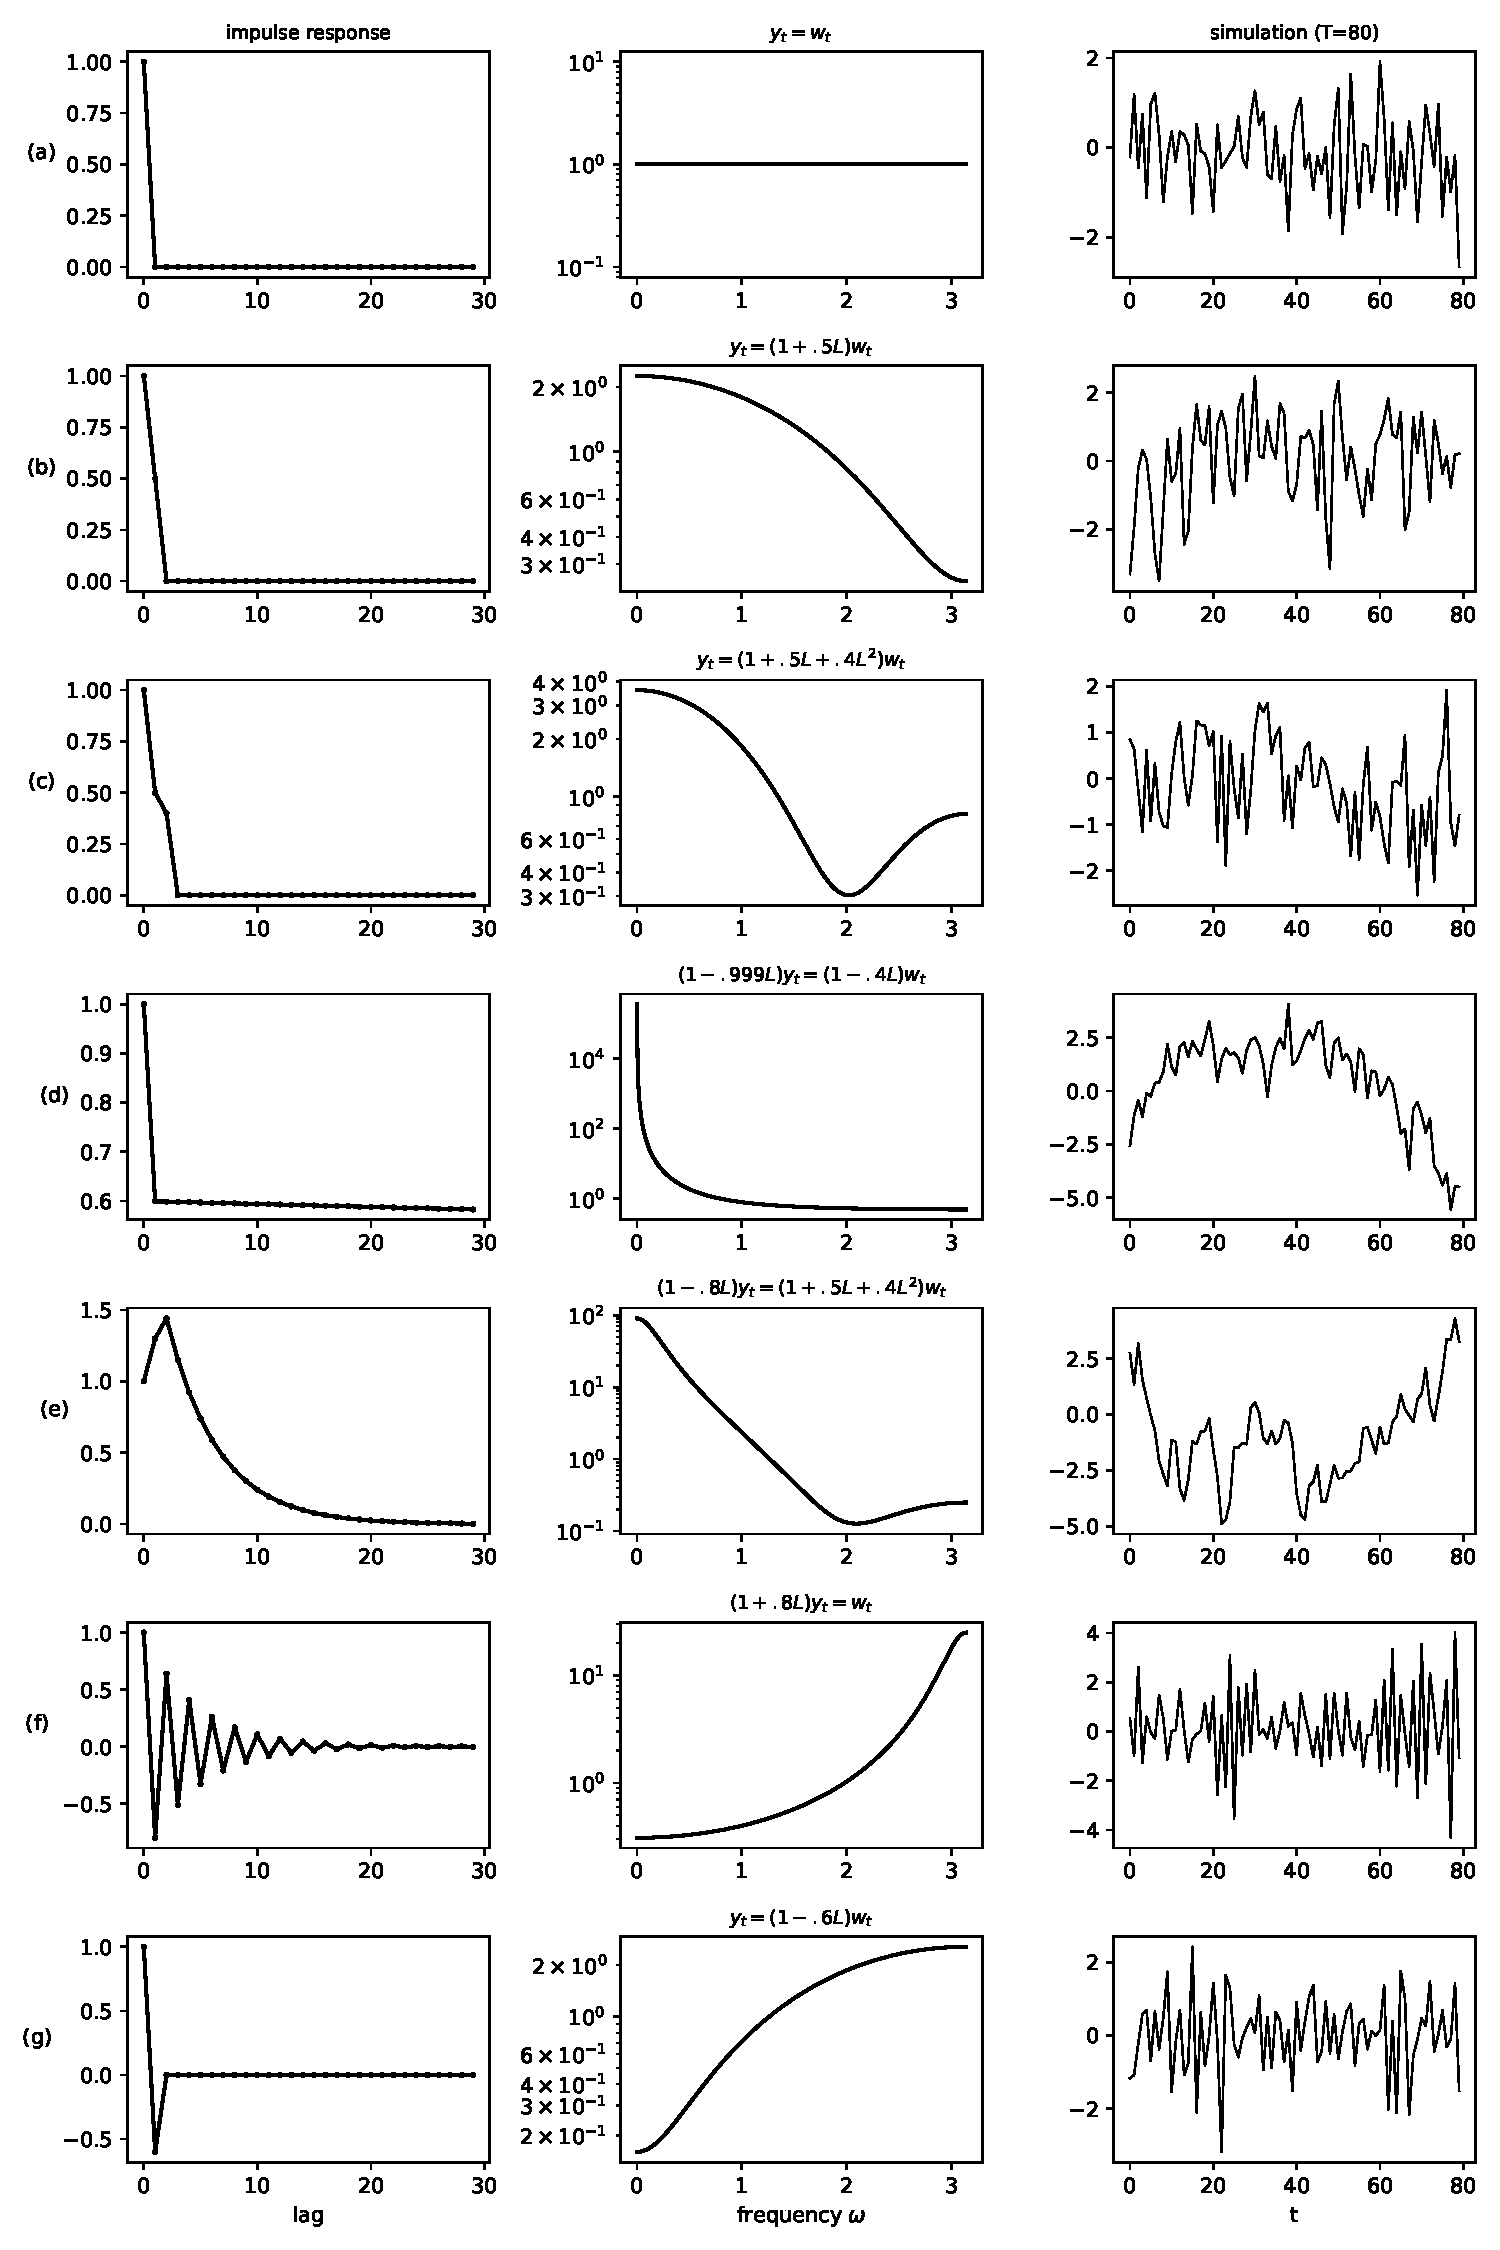
\includegraphics[width=0.93\textwidth,height=0.82\textheight,keepaspectratio]{figures/ch2_07.pdf}\\
{\small Figure S2.1. Impulse responses, spectra (log scale, $0\le\omega\le\pi$) and simulated paths.}
\end{center}
Patterns:
\begin{itemize}[leftmargin=*]
\item White noise (a) has a flat spectrum: all frequencies contribute equally, and the path has no visible structure.
\item Positive moving-average coefficients, as in (b) and (c), smooth the process.  They move variance toward low frequencies:
$S(0)=b(1)^2$ (2.25 and 3.61) exceeds $S(\pi)=b(-1)^2$ (0.25 and 0.81).  In (c) the zero of $|b(e^{-i\omega})|$ near $\omega\approx2$ carves a trough.
A negative coefficient, as in (g), does the opposite: $S(0)=0.16$, $S(\pi)=2.56$, and the path looks choppier than white noise.
\item A near unit root, as in (d), produces an enormous spectral peak at frequency zero ($S(0)\approx3.6\times10^5$).  The impulse response is
$1$ on impact and then an almost permanent $0.6$.  The simulated path wanders like a random walk.  This is Granger's ``typical spectral
shape''.
\item Combining a persistent AR with a smoothing MA, as in (e), gives a hump-shaped impulse response (it rises before it decays) and a spectrum
that declines steeply in $\omega$.
\item A negative AR root, as in (f), produces an oscillating impulse response ($(-.8)^j$) and a spectrum that rises toward
$\omega=\pi$, the two-period cycle.  The path alternates in sign.
\end{itemize}
In short: the spectrum records at which frequencies a process has its variance, and the impulse response tells the same story in the time
domain.  Smooth, persistent responses mean low-frequency power; oscillating responses mean high-frequency power.
\end{ex}

%%---------------------------------------------------------------------------
\begin{ex}{2.8}{Cagan's money demand under perfect foresight}
\exnote{Equation (4) refers to a numbered display of the exercise in the book.}
Let $\lambda=\alpha/(1+\alpha)\in(0,1)$.  The demand function can be written $p_t=(1-\lambda)m_t+\lambda p_{t+1}$.

\textbf{(a)}  \emph{A particular solution.}  Try $p_t=w_0m_t+w_1m_{t-1}$.  Substituting, and using $m_{t+1}=(1+\rho)m_t-\rho m_{t-1}$, gives
\[
  (1-w_0)m_t-w_1m_{t-1}=-\alpha\,(w_0\rho+w_1)(m_t-m_{t-1}).
\]
Matching coefficients: $w_0+w_1=1$ and $w_1(1+\alpha)=-\alpha\rho w_0$, i.e.\ $w_1=-\lambda\rho w_0$.  Hence
\[
  w_0=\frac1{1-\lambda\rho},\qquad w_1=-\frac{\lambda\rho}{1-\lambda\rho},\qquad w_j=0\ (j\ge2),
  \qquad p^{*}_t=\frac{m_t-\lambda\rho\,m_{t-1}}{1-\lambda\rho}.
\]
The same formula follows from solving forward: $p^*_t=(1-\lambda)\sum_{j\ge0}\lambda^jm_{t+j}$.  Write $m_{t+j}=k_1+k_2\rho^{t+j}$ ($\rho\ne1$), with the
constants expressed through $m_t,m_{t-1}$, and sum the two geometric series.

\emph{All solutions.}  The difference $f_t=p_t-p^*_t$ of any two solutions satisfies the homogeneous equation $-f_t=-\alpha(f_{t+1}-f_t)$, i.e.\
$f_{t+1}=\lambda^{-1}f_t=\frac{1+\alpha}{\alpha}f_t$.  So every equilibrium is
\[
  p_t=\frac{m_t-\lambda\rho\,m_{t-1}}{1-\lambda\rho}+f_0\Bigl(\frac{1+\alpha}{\alpha}\Bigr)^{t},\qquad f_0\in\R\ \text{arbitrary}.
\]

\textbf{(b)}  There is a continuum of equilibria, one for each $f_0$ (equivalently, each initial price level $p_0$).  Every equilibrium with $f_0\ne0$
contains a ``bubble'' growing at the gross rate $(1+\alpha)/\alpha>1$.

\textbf{(c)}  Yes: $f_0=0$ gives $p_t=p^*_t$.  It is the unique equilibrium in which the price level equals the discounted value of current and future money
supplies, and hence the only one without an explosive bubble relative to $m$.

\textbf{(d)}  The undetermined-coefficients formula for $(w_0,w_1)$ only needs $\lambda\rho\ne1$.  Condition (4), $|\lambda\rho|<1$, is what makes the
forward sum $(1-\lambda)\sum_j\lambda^jm_{t+j}$ converge when money grows like $\rho^t$.  So it is needed to interpret $p^*_t$ as a present
value, and to single out $f_t=0$ as the ``no-bubble'' solution by a transversality-type argument.

\textbf{(e)}  With $\alpha=1$, $\lambda=\frac12$, and $\rho=1$ (condition (4) holds: $\lambda\rho=\frac12$):
\[
  p_t=2m_t-m_{t-1}+f_0\,2^t=m_t+(m_t-m_{t-1})+f_0\,2^t .
\]
Money grows linearly, $m_t=m_{-1}+(t+1)(m_{-1}-m_{-2})$.  The fundamental price level is money plus $\alpha$ times the (constant) inflation rate,
since real balances equal $-\alpha$ times inflation.  Figure S2.2 plots the fundamental solution (solid) and four bubble equilibria
($f_0=\pm.01,\pm.02$, dashed) for $m_{-2}=0$, $m_{-1}=1$, so that $m_t=t+2$ and $p^*_t=t+3$.
\begin{center}
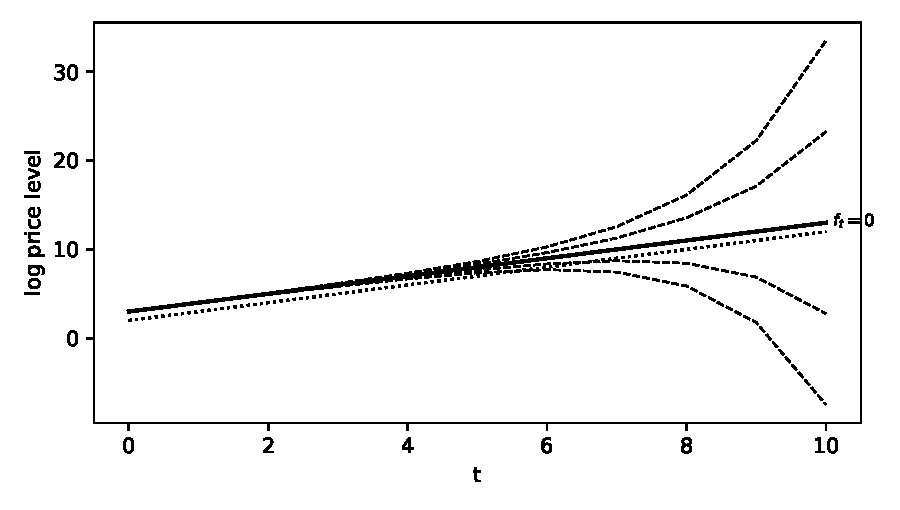
\includegraphics[width=0.62\textwidth]{figures/ch2_08.pdf}\\
{\small Figure S2.2. Equilibria of the Cagan model with $\alpha=\rho=1$; dotted: $m_t$.}
\end{center}
\end{ex}

%%---------------------------------------------------------------------------
\begin{ex}{2.9}{Pricing a one-period payoff with a linear stochastic discount factor}
\textbf{(a)}  $m_{t+1}p_{t+1}=\dfrac{(Mx_{t+1})(Px_{t+1})}{Mx_t}=\dfrac{x_{t+1}'M'Px_{t+1}}{Mx_t}$.  Using $E_tx_{t+1}=Ax_t$ and
$E_t(x_{t+1}-Ax_t)(x_{t+1}-Ax_t)'=C_tC_t'$,
\[
  q_t=f_t(x_t)=\frac{(MAx_t)(PAx_t)+PC_tC_t'M'}{Mx_t}
  =\underbrace{\frac{MAx_t}{Mx_t}}_{E_tm_{t+1}}\,\underbrace{PAx_t}_{E_tp_{t+1}}+\underbrace{\frac{PC_tC_t'M'}{Mx_t}}_{\cov_t(m_{t+1},p_{t+1})}.
\]
(This requires $Mx_t\neq0$.)  The price is the risk-neutral value $E_tm\cdot E_tp$ plus a risk adjustment equal to the conditional covariance of the
discount factor with the payoff.  $A$ enters through the conditional means and $C_t$ through the covariance, and the time variation of
$C_t$ is why the pricing function carries a $t$ subscript.

\textbf{(b)}  Let $e_{t+1}=m_{t+1}p_{t+1}-q_t$.  The model says $E(e_{t+1}\given J_t)=0$.  The econometrician's information $z^t=(z_t,z_{t-1},\dots)$ is
contained in $J_t$, so by the law of iterated expectations $E(e_{t+1}\given z^t)=0$.  Hence $E[h(z^t)e_{t+1}]=0$ for every function $h$ of the
econometrician's information.  Choose a vector of instruments $h_t$ (a constant, $z_t$, lags, squares), form the sample moments
$g_T=T^{-1}\sum_th_te_{t+1}$, and test $Eh_te_{t+1}=0$ with Hansen's $J$ statistic
$Tg_T'\hat S^{-1}g_T\to\chi^2_{\dim h}$, where $\hat S=T^{-1}\sum_th_th_t'e_{t+1}^2$.  Because $e_{t+1}$ is a martingale difference, no
autocorrelation correction is needed.  Equivalently, regress $e_{t+1}$ on $h_t$ and test that all coefficients are zero with robust
standard errors.  The econometrician does not need to see all of $x_t$: omitted state variables only reduce the power of the test, not its validity.
\end{ex}

%%---------------------------------------------------------------------------
\begin{ex}{2.10}{Mixtures of invariant distributions}
Let $\pi_\alpha=\alpha\pi_1+(1-\alpha)\pi_2$.  By linearity, $P'\pi_\alpha=\alpha P'\pi_1+(1-\alpha)P'\pi_2=\alpha\pi_1+(1-\alpha)\pi_2=\pi_\alpha$.  Its components are
nonnegative, since they are convex combinations of nonnegative numbers, and they sum to $\alpha\cdot1+(1-\alpha)\cdot1=1$.  So $\pi_\alpha$ is a
probability vector satisfying $\pi_\alpha=P'\pi_\alpha$, i.e.\ an invariant distribution.  The set of invariant distributions is convex.
\end{ex}

%%---------------------------------------------------------------------------
\begin{ex}{2.11}{Distributions over time for a chain with two absorbing states}
From $\pi_{t+1}'=\pi_t'P$, component by component:
$\pi_{1,t+1}=\pi_{1t}+.2\pi_{2t}$, $\pi_{2,t+1}=.5\pi_{2t}$, $\pi_{3,t+1}=\pi_{3t}+.3\pi_{2t}$.  The middle equation gives $\pi_{2t}=.5^t\pi_{2,0}$.
Substituting into the first and summing,
\[
  \pi_{1t}=\pi_{1,0}+.2\sum_{s=0}^{t-1}\pi_{2s}=\pi_{1,0}+.2\,\pi_{2,0}\sum_{s=0}^{t-1}.5^s=\pi_{1,0}+.2\,\frac{1-.5^t}{1-.5}\,\pi_{2,0},
\]
and identically for $\pi_{3t}$ with $.3$ in place of $.2$.  (Formally, each formula is proved by induction on $t$, using the one-step recursion.)
As $t\to\infty$ the transient state 2 empties, $\pi_{1\infty}=\pi_{1,0}+.4\pi_{2,0}$ and $\pi_{3\infty}=\pi_{3,0}+.6\pi_{2,0}$.
\end{ex}

%%---------------------------------------------------------------------------
\begin{ex}{2.12}{Columns of powers of $P'$}
The distribution evolves as $\pi_{t+1}=P'\pi_t$, so $\pi_t=(P')^t\pi_0$ by induction.  With $\pi_0=e_j$, $\pi_t=(P')^te_j$, which is the $j$th column of
$(P')^t$.  Equivalently, the $(i,j)$ element of $(P')^t$ is $(P^t)_{ji}=\Prob(x_t=e_i\given x_0=e_j)$.
\end{ex}

%%---------------------------------------------------------------------------
\begin{ex}{2.13}{A permanent income problem solved by Howard's algorithm}
\textbf{(a)}  The budget constraint gives $b_{t+1}=\beta^{-1}(u_t+30+b_t-y_t)$, and $y_{t+1}=.5+1.3y_t-.4y_{t-1}+.05w_{t+1}$.  Hence
$x_{t+1}=Ax_t+Bu_t+Cw_{t+1}$ with
\[
  A=\begin{bmatrix}1&0&0&0\\30/\beta&1/\beta&-1/\beta&0\\.5&0&1.3&-.4\\0&0&1&0\end{bmatrix},\qquad
  B=\begin{bmatrix}0\\1/\beta\\0\\0\end{bmatrix},\qquad C=\begin{bmatrix}0\\0\\.05\\0\end{bmatrix}.
\]
$A$ is block triangular.  Its eigenvalues are $1$ (the constant), $1/\beta=1.0526$ (debt compounds at the gross interest rate) and the roots
of $\lambda^2-1.3\lambda+.4=0$, namely $0.8$ and $0.5$.  The zeros of $1-1.3z+.4z^2$ are $1.25$ and $2$, the reciprocals of $0.8$ and $0.5$.  The one-period loss is
$x_t'Rx_t+u_t'Qu_t$ (scaled by $.5$) with $R=\diag(0,10^{-6},0,0)$ and $Q=1$.

\textbf{(b)}  Howard's algorithm needs an initial rule $F_0$ for which $\sqrt\beta(A-BF_0)$ is stable.  We use $u_t=-(1-\beta)b_t$, which makes debt a
unit-root process ($b_{t+1}=b_t+(30-y_t)/\beta$).  Then $\sqrt\beta(A-BF_0)$ has spectral radius $0.975$.  Iterating on \bk{(2.4.30)}, alternately
solving the Lyapunov equation for $P_j$ and updating $F_{j+1}=\beta(Q+\beta B'P_jB)^{-1}B'P_jA$, converges in \textbf{3 improvement steps} with
the criterion $\max|F_{j+1}-F_j|<10^{-10}\max|F_{j+1}|$.  The same answer (to $6\times10^{-14}$) takes 820 iterations of the Riccati recursion
\bk{(2.4.31)}, which illustrates the speed of Howard's algorithm.  The optimal rule is
\[
  c_t=30-F^*x_t=3.7695-0.050019\,b_t+0.396944\,y_t-0.150836\,y_{t-1}.
\]
At $b_t=0$ and $y_t=y_{t-1}=5$ this gives $c_t=5$, and the coefficient on debt is essentially $-(1-\beta)=-0.05$, the permanent income rule.

\textbf{(c)}  The eigenvalues of $A-BF^*$ are $0.5,\;0.8,\;0.99998,\;1$.  The explosive debt root has been replaced by a root just below one.  The
tiny penalty $10^{-6}b_t^2$ makes debt, and hence consumption, very slowly mean-reverting.  Figure S2.3 compares the impulse responses with
the theoretical ones from \bk{(2.12.18)}, where $z_t=(1,y_t,y_{t-1})'$, $U_y=(0,1,0)$ and
$(1-\beta)U_y(I-\beta A_{22})^{-1}C_2=(1-\beta)\,.05/(1-1.3\beta+.4\beta^2)=0.019841$.
\begin{center}
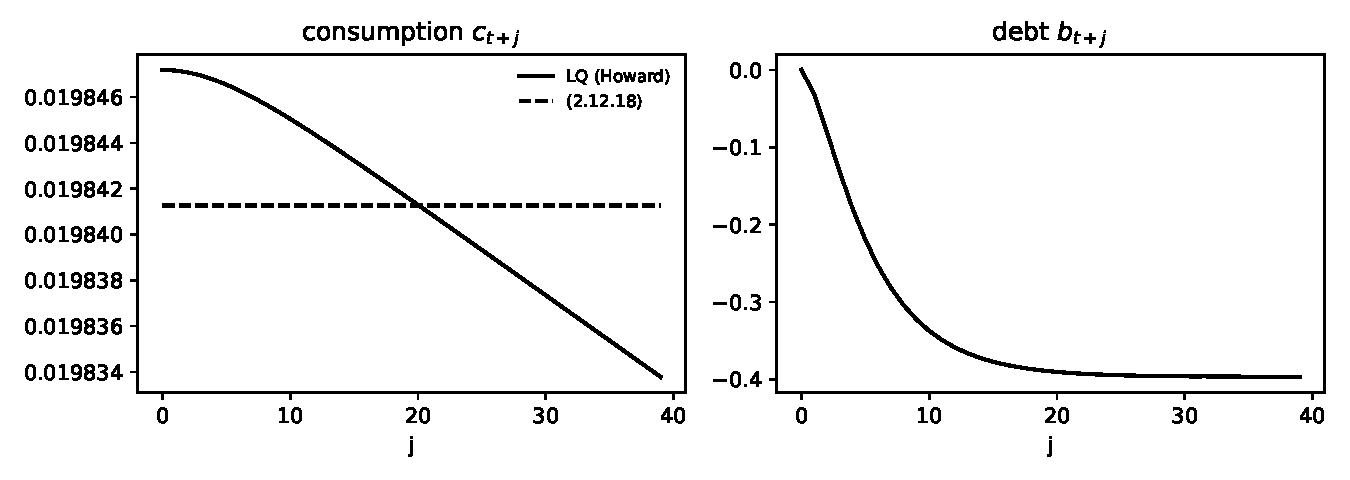
\includegraphics[width=0.85\textwidth]{figures/ch2_13.pdf}\\
{\small Figure S2.3. Responses of $c_{t+j}$ and $b_{t+j}$ to $w_{t+1}=1$: optimal LQ rule (solid) and formula (2.12.18) (dashed).}
\end{center}
Consumption jumps by $0.019847$ on impact (theory: $0.019841$) and stays there: $0.019834$ after 40 periods.  Debt falls by the amounts theory
predicts ($-0.03174$ after one period, $-0.21971$ after five, $-0.39643$ after 39, versus $-0.03175$, $-0.21974$, $-0.39673$).  Up to the
$10^{-6}$ penalty, the LQ solution \emph{is} the permanent income model: consumption is a random walk that moves by $(1-\beta)$ times
the revision in the present value of income.
\end{ex}

%%---------------------------------------------------------------------------
\begin{ex}{2.14}{A chain with a closed class, a transient state and an absorbing state}
\textbf{(a)}  States $\{1,2\}$ form a closed class, state 3 is transient (it leaks to 4) and state 4 is absorbing.  On $\{1,2\}$,
$\pi_1=.5\pi_1+.1\pi_2$ gives $\pi_2=5\pi_1$, i.e.\ $(1/6,5/6)$.  State 3 gets no mass in any stationary distribution, since
$\pi_3=.9\pi_3$.  The stationary distributions are
\[
  \pi^{(\gamma)}=\gamma\,(\tfrac16,\tfrac56,0,0)'+(1-\gamma)\,(0,0,0,1)',\qquad\gamma\in[0,1].
\]

\textbf{(b)}  Invariant functions solve $P\bar y=\bar y$: $\bar y_1=\bar y_2$ and $\bar y_3=\bar y_4$, so $\bar y=(a,a,b,b)'$.  The chain is ergodic under
$\pi^{(\gamma)}$ if every invariant function is constant on the support of $\pi^{(\gamma)}$.  This holds for $\gamma=1$ (support $\{1,2\}$) and
$\gamma=0$ (support $\{4\}$), but not for $\gamma\in(0,1)$, where $(a,a,b,b)$ with $a\ne b$ is invariant and non-constant.  So yes: the extreme
points $(\frac16,\frac56,0,0)$ and $(0,0,0,1)$ make the chain ergodic.

\textbf{(c)}  A path that starts in $\{1,2\}$ stays there, and by the ergodic theorem its sample mean converges to
$1\cdot\frac16+2\cdot\frac56=\frac{11}6$.  A path that starts in 3 or 4 is absorbed in state 4 in finite time (with probability one), so its sample mean
converges to $4$.  The possible limits are $11/6$ and $4$.  The limit is $11/6$ with probability $\pi_{0,1}+\pi_{0,2}$ and $4$ with probability
$\pi_{0,3}+\pi_{0,4}$.
\end{ex}

%%---------------------------------------------------------------------------
\begin{ex}{2.15}{The Slutsky effect}
$|1+e^{-i\omega}|^2=2+2\cos\omega=4\cos^2(\omega/2)$ and $|1-e^{-i\omega}|^2=2-2\cos\omega=4\sin^2(\omega/2)$, so
\[
  S_y(\omega)=4^{m+n}\cos^{2n}(\omega/2)\,\sin^{2m}(\omega/2).
\]
Setting the derivative of $n\log\cos^2(\omega/2)+m\log\sin^2(\omega/2)$ to zero gives $\tan^2(\omega/2)=m/n$: the spectrum has a single peak (on each side
of zero) at
\[
  \omega^*=2\arctan\sqrt{m/n}.
\]
\begin{center}
\begin{tabular}{lcccc}
\toprule
$(m,n)$ & $(10,10)$ & $(10,40)$ & $(40,10)$ & $(120,30)$\\
\midrule
peak $\omega^*$ & $1.571$ & $0.927$ & $2.214$ & $2.214$\\
period $2\pi/\omega^*$ & $4.00$ & $6.78$ & $2.84$ & $2.84$\\
width at half power & $0.523$ & $0.330$ & $0.330$ & $0.190$\\
\bottomrule
\end{tabular}
\end{center}
\begin{center}
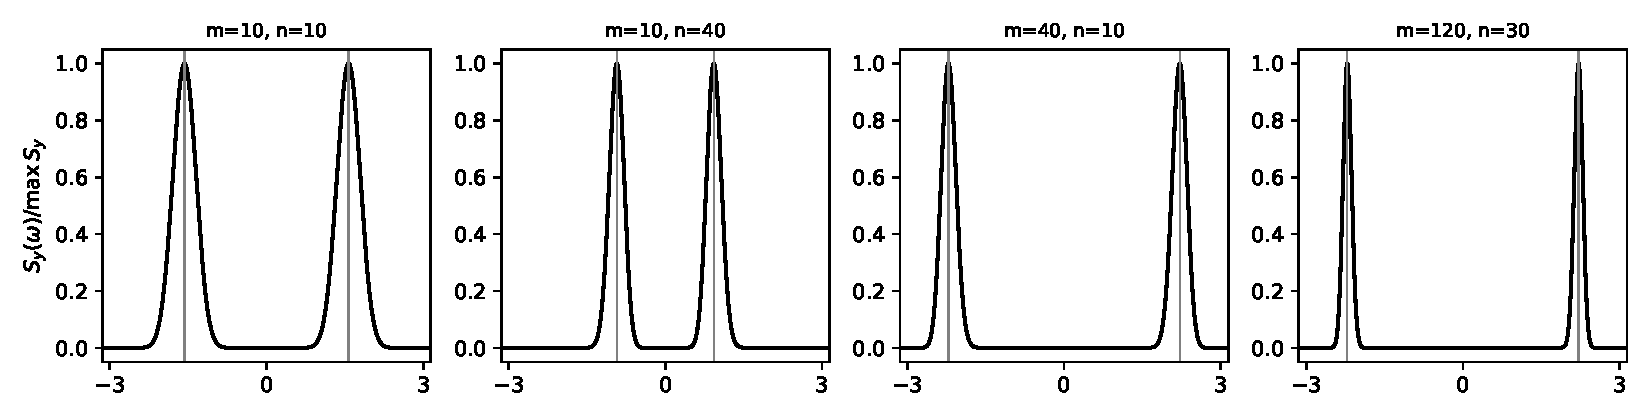
\includegraphics[width=\textwidth]{figures/ch2_15.pdf}\\
{\small Figure S2.4. Normalized spectra $S_y(\omega)/\max S_y$ on $[-\pi,\pi]$; vertical lines at $\pm\omega^*$.}
\end{center}
\emph{Comment.}  Summing ($1+L$) is a low-pass filter and differencing ($1-L$) a high-pass filter.  Their product is a band-pass filter.  Applied
many times, it concentrates almost all the variance of pure white noise in a narrow band around $\omega^*$, set by the ratio $m/n$.  The band
narrows as $m+n$ grows (compare $(40,10)$ with $(120,30)$, which share $\omega^*$).  The filtered series therefore displays strikingly regular
``cycles'' of period $2\pi/\omega^*$, although the input has no cyclical structure at all.  This is the Slutsky--Yule effect: cycles in data can be
artifacts of the filters (sums and differences) applied to random shocks.
\end{ex}

%%---------------------------------------------------------------------------
\begin{ex}{2.16}{A law of large numbers for indicator functions}
\textbf{(a)}  Under the stationary distribution, $\Prob(x_t=e_i)=\pi_i$ for every $t$, so $EI_{it}=1\cdot\pi_i+0\cdot(1-\pi_i)=\pi_i$.

\textbf{(b)}  $I_{it}=\bar y'x_t$ with $\bar y=e_i$ is a function of the state.  Since $(P,\pi)$ is stationary and ergodic, the law of large numbers
\bk{Theorem 2.2.5} gives $\frac1T\sum_tI_{it}\to EI_{i0}=\pi_i$ with probability one.  For a self-contained argument:
\begin{itemize}[leftmargin=*]
\item If $\pi_i=0$, then $\Prob(x_t=e_i)=0$ for all $t$, so $I_{it}=0$ almost surely and the average is $0=\pi_i$.
\item If $\pi_i>0$: with a unique stationary distribution, a finite chain has exactly one closed communicating class, which is the support of $\pi$.
Started from $\pi$, the chain lives on that class, where it is irreducible and positive recurrent.  The times between successive visits to $e_i$
are then i.i.d.\ with some finite mean $m_i$.  The strong law of large numbers applied to these cycle lengths gives
$\frac1T\#\{t<T:x_t=e_i\}\to1/m_i$ almost surely.  By bounded convergence, $1/m_i=\lim_T\frac1T\sum_tEI_{it}=\pi_i$ (Kac's formula).
\end{itemize}
\end{ex}

%%---------------------------------------------------------------------------
\begin{ex}{2.17}{The lake model}
\textbf{(a)}  $P=\begin{bmatrix}1-\lambda&\lambda\\\delta&1-\delta\end{bmatrix}$.  Stationarity requires $\pi_u\lambda=\pi_e\delta$ (flows into and out of unemployment
balance), so the unique stationary distribution is
\[
  \pi_u=\frac{\delta}{\lambda+\delta},\qquad \pi_e=\frac{\lambda}{\lambda+\delta}.
\]
All entries of $P$ are positive, so by \bk{Theorem 2.2.1} the chain is asymptotically stationary.  The only invariant functions are constants, since
$P\bar y=\bar y$ forces $\bar y_1=\bar y_2$, so the chain is ergodic under $\pi$.

\textbf{(b)}  $\pi_u=.25/.30=0.8333$ and $\pi_e=0.1667$.  By the ergodic theorem, the fraction of an infinitely long life spent unemployed is $\pi_u=5/6$.

\textbf{(c)}  $g_{ij}=\pi_jP_{ji}$: $g_{11}=\pi_u(1-\lambda)=0.79167$, $g_{21}=\pi_u\lambda=0.04167$, $g_{12}=\pi_e\delta=0.04167$, $g_{22}=\pi_e(1-\delta)=0.125$.
In a stationary lake, the flows out of and into unemployment are equal ($g_{21}=g_{12}$).

\textbf{(d)}  The pair $(x_t,x_{t-1})$ is itself a stationary ergodic Markov chain, so by the ergodic theorem $\frac1T\sum_tI_{ij,t}\to g_{ij}$ almost surely,
with the values in (c).

\textbf{(e)}  Since $\lambda=g_{21}/(g_{11}+g_{21})$ and $\delta=g_{12}/(g_{12}+g_{22})$, replace population moments by sample frequencies.  Let $n_{ij}$ be the
number of transitions from $j$ to $i$; for instance, $n_{21}$ counts transitions from unemployment into employment.  Then
\[
  \hat\lambda=\frac{n_{21}}{n_{11}+n_{21}},\qquad \hat\delta=\frac{n_{12}}{n_{12}+n_{22}},\qquad \hat{\bar w}=F^{-1}(1-\hat\lambda),
\]
the last because $\lambda=1-F(\bar w)$.  It is unique if $F$ is strictly increasing near $\bar w$.

\textbf{(f)}  Conditional on $x_0$, the likelihood of a sample is
$(1-\lambda)^{n_{11}}\lambda^{n_{21}}\delta^{n_{12}}(1-\delta)^{n_{22}}$.  Maximizing, $\hat\lambda^{ML}=n_{21}/(n_{11}+n_{21})$ and $\hat\delta^{ML}=n_{12}/(n_{12}+n_{22})$.

\textbf{(g)}  They are identical.  (If the likelihood also includes $\Prob(x_0)=\pi_{x_0}$, the MLE differs from the method of moments estimator by
a term of order $1/T$.)

\textbf{(h)}  The per-period log likelihood contributes information $\pi_u/[\lambda(1-\lambda)]$ about $\lambda$ and $\pi_e/[\delta(1-\delta)]$ about $\delta$,
with no cross term.  Hence
\[
  \sqrt T\begin{pmatrix}\hat\lambda-\lambda\\\hat\delta-\delta\end{pmatrix}\to\Norm\!\left(0,\;
  \begin{bmatrix}\lambda(1-\lambda)/\pi_u&0\\0&\delta(1-\delta)/\pi_e\end{bmatrix}\right)
  =\Norm\!\left(0,\;\begin{bmatrix}0.0570&0\\0&1.1250\end{bmatrix}\right)
\]
at $\lambda=.05$, $\delta=.25$.  $\delta$ is estimated much less precisely: a worker spends only one-sixth of the time employed, which is when firing
can be observed.
\end{ex}

%%---------------------------------------------------------------------------
\begin{ex}{2.18}{Gambler's ruin}
\textbf{(a)}  States 1 and 4 are absorbing, and 2 and 3 are transient.  The stationary distributions are $\gamma e_1+(1-\gamma)e_4$, $\gamma\in[0,1]$.

\textbf{(b)}  $P\bar y=\bar y$ requires $\bar y_2=\frac12(\bar y_1+\bar y_3)$ and $\bar y_3=\frac12(\bar y_2+\bar y_4)$, i.e.\ $\bar y$ is affine in the index.  The invariant
functions form the two-dimensional space $\bar y_i=a+bi$.  The chain is ergodic only for $\gamma\in\{0,1\}$: for $\gamma\in(0,1)$ the invariant function
$\bar y_i=i$ is not constant on the support $\{1,4\}$.

\textbf{(c)}  $P\bar y=(1,\;.5\cdot1+.5\cdot3,\;.5\cdot2+.5\cdot4,\;4)'=(1,2,3,4)'$.  So $E[y_{t+1}\given x_t]=y_t$ in every state: $y_t$ is a martingale.

\textbf{(d)}  Condition \bk{(2.2.12)} holds, and $\bar y$ is a right eigenvector of $P$ with unit eigenvalue (\bk{(2.2.13)}).  Under \emph{any
stationary} distribution, the chain sits in state 1 or 4 forever, so $y_t$ is constant along every path of positive probability: it is invariant, as
\bk{Theorem 2.2.4} asserts.  But from the transient states 2 or 3, $y_t$ moves until absorption.  Such initial conditions are not
stationary distributions, and stationarity of $(P,\pi)$ is the hypothesis of \bk{Theorem 2.2.4} that fails.  A martingale need not be constant
if the chain is not started from its stationary distribution.

\textbf{(e)}  $y_t$ is a bounded martingale, so it converges almost surely by the martingale convergence theorem.  Directly: from state 2 or 3 the chain
is absorbed next period with probability $1/2$, so absorption happens in finite time almost surely, and $y_t\to y_\infty\in\{1,4\}$.
Optional stopping gives $E[y_\infty\given x_0=e_i]=i$, so $\Prob(y_\infty=4\given x_0=e_i)=(i-1)/3$ and $\Prob(y_\infty=1\given x_0=e_i)=(4-i)/3$.  Starting from
state 2, for instance, $y_t\to4$ with probability $1/3$ and $\to1$ with probability $2/3$.
\end{ex}

%%---------------------------------------------------------------------------
\begin{ex}{2.19}{Learning a person's IQ}
\textbf{(a)}  This is the Kalman filter \bk{(2.10.8)} with $A=1$, $C=0$, $G=1$, $R=100$, $\hat x_0=100$, $\Sigma_0=100$.  With $\Sigma_t=E(IQ_t-\theta)^2$,
\[
  IQ_{t+1}=IQ_t+K_t(y_t-IQ_t),\qquad K_t=\frac{\Sigma_t}{\Sigma_t+100},\qquad \Sigma_{t+1}=\frac{100\,\Sigma_t}{\Sigma_t+100}.
\]
In precision form, $1/\Sigma_{t+1}=1/\Sigma_t+1/100$, so $\Sigma_t=100/(t+1)$ and $K_t=1/(t+2)$.  Solving the recursion,
\[
  IQ_t=\frac{100+\sum_{s=0}^{t-1}y_s}{t+1}:
\]
the prior mean counts as one extra test score, because the prior variance equals the variance of a single test.

\textbf{(b)}  See Figure S2.5 (\texttt{code/ch2.py}).
\begin{center}
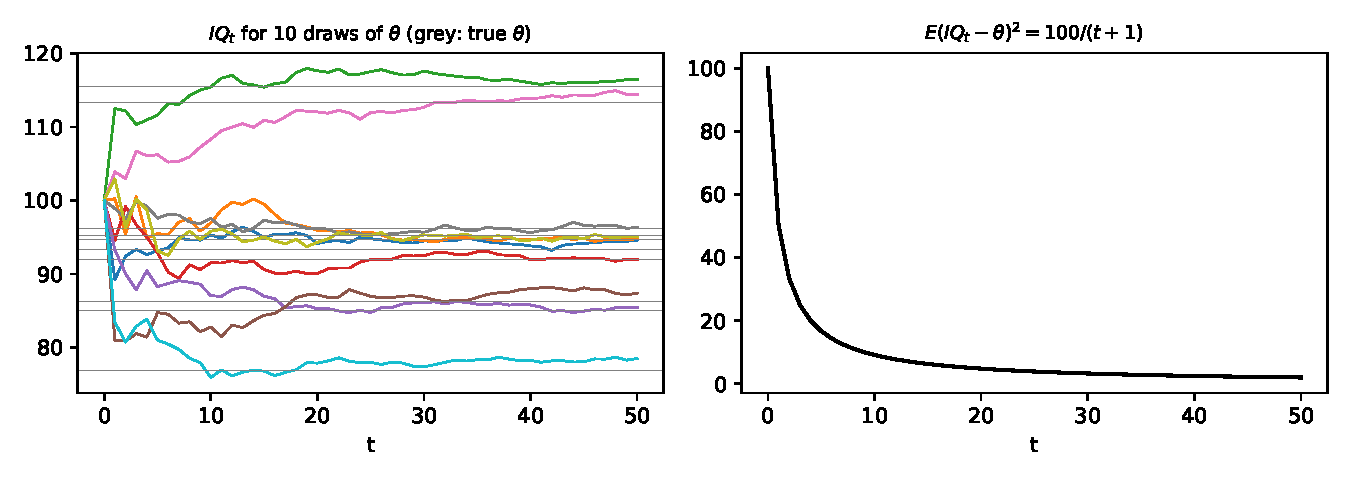
\includegraphics[width=0.9\textwidth]{figures/ch2_19.pdf}\\
{\small Figure S2.5. Simulated $IQ_t$ paths for 10 persons (left) and the mean squared error $100/(t+1)$ (right).}
\end{center}

\textbf{(c)}  $E(IQ_t-\theta)^2=\Sigma_t=100/(t+1)\to0$.  The estimate is consistent in mean square, although it converges only at rate $t^{-1/2}$.
\end{ex}

%%---------------------------------------------------------------------------
\begin{ex}{2.20}{Two noisy signals on a random walk}
\textbf{(a)}  With $A=1$, $C=1$, $G=\iota=(1,1)'$ and $R=I$, we have $(\Sigma\iota\iota'+I)^{-1}=I-\frac{\Sigma}{1+2\Sigma}\iota\iota'$.  The Riccati equation
\bk{(2.7.15)} becomes
\[
  \Sigma_{t+1}=\Sigma_t+1-\Sigma_t^2\,\iota'(\Sigma_t\iota\iota'+I)^{-1}\iota=\frac{1+3\Sigma_t}{1+2\Sigma_t}.
\]
Its fixed point solves $2\Sigma^2-2\Sigma-1=0$, i.e.\ $\Sigma=(1+\sqrt3)/2=1.36602540378444$, exactly the given $\Sigma_0$.  So the filter is time
invariant from the start, with gain
\[
  K=\Sigma\iota'(\Sigma\iota\iota'+I)^{-1}=\frac{\Sigma}{1+2\Sigma}\,(1,1)=\tfrac{\sqrt3-1}{2}(1,1)=(0.36603,\;0.36603).
\]
Hence $\hat x_{t+1}=(1-2k)\hat x_t+k(y_{1t}+y_{2t})$ with $k=(\sqrt3-1)/2$ and $1-2k=2-\sqrt3$, and
\[
  E[x_t\given y^{t-1}]=\hat x_t=(2-\sqrt3)^t\hat x_0+\tfrac{\sqrt3-1}{2}\sum_{j=0}^{t-1}(2-\sqrt3)^j\,(y_{1,t-1-j}+y_{2,t-1-j}).
\]
The two signals enter symmetrically through their sum, and $E[x_{t+j}\given y^{t-1}]=\hat x_t$ for all $j\ge0$ because $x$ is a random walk.

\textbf{(b)}  $A-KG=1-2k=2-\sqrt3=0.26795$, inside the unit circle (confirmed numerically by \texttt{ch2.py}).

\textbf{(c)}  From \bk{(2.9.3)}, $y_t=G\sum_{j\ge0}(A-KG)^jKy_{t-j-1}+a_t$, i.e.
\[
  y_t=\sum_{j=1}^\infty\tfrac{\sqrt3-1}{2}(2-\sqrt3)^{j-1}\begin{bmatrix}1&1\\1&1\end{bmatrix}y_{t-j}+a_t,\qquad
  Ea_ta_t'=\Sigma\iota\iota'+I=\begin{bmatrix}2.36603&1.36603\\1.36603&2.36603\end{bmatrix}.
\]
\end{ex}

%%---------------------------------------------------------------------------
\begin{ex}{2.21}{Impulse response of a VAR}
Iterating $\hat x_{t+1}=A\hat x_t+Ka_t$ and $y_t=G\hat x_t+a_t$ gives the moving-average representation
\[
  y_t=a_t+\sum_{j\ge1}GA^{j-1}K\,a_{t-j},\qquad\text{i.e.}\qquad y_t=\bigl[I+G(I-AL)^{-1}KL\bigr]a_t .
\]
The response of $y_{t+j}$ to $a_t$ is $I$ for $j=0$ and $GA^{j-1}K$ for $j\ge1$.  For the state, the response of $\hat x_{t+j}$ is $A^{j-1}K$.  If one wants
responses to orthogonal shocks, write $a_t=\Omega^{1/2}\varepsilon_t$ with $\Omega=Ea_ta_t'$ (e.g.\ a Cholesky factor) and post-multiply the
responses by $\Omega^{1/2}$.
\end{ex}

%%---------------------------------------------------------------------------
\begin{ex}{2.22}{Kalman filter with correlated shocks}
\textbf{(a)}  $E(Cw_{t+1})(Dw_{t+1})'=CD'$.  Partition $w=(w_1',w_2')'$ and set $C=[C_1\;0]$, $D=[0\;D_2]$.  Then $CD'=0$: the state shocks and
measurement errors are driven by different components of $w$, as in the setup of section \bk{2.7}.  \emph{Correlated example:} an MA(1),
$y_{t+1}=w_{t+1}+\theta w_t$.  Take $x_t=w_t$, $A=0$, $C=1$, $G=\theta$, $D=1$.  Then $Cw_{t+1}=Dw_{t+1}=w_{t+1}$ and $CD'=1\ne0$.

\textbf{(b)}  Let $\tilde x_t=x_t-\hat x_t$.  Because $w_{t+1}$ is independent of $(x_t,y^t)$, $E[y_{t+1}\given y^t]=G\hat x_t$, so
\[
  a_{t+1}=y_{t+1}-G\hat x_t=G\tilde x_t+Dw_{t+1},\qquad Ea_{t+1}a_{t+1}'=G\Sigma_tG'+DD'.
\]
The information in $y^{t+1}$ equals the information in $(y^t,a_{t+1})$, with $a_{t+1}$ orthogonal to $y^t$.  So, by the population regression formula (with
Gaussian shocks, projections are conditional expectations),
\[
  \hat x_{t+1}=E[x_{t+1}\given y^t]+\cov(x_{t+1},a_{t+1})\,[\var(a_{t+1})]^{-1}a_{t+1}.
\]
Here $E[x_{t+1}\given y^t]=A\hat x_t$ and
$\cov(x_{t+1},a_{t+1})=E(A\tilde x_t+Cw_{t+1})(G\tilde x_t+Dw_{t+1})'=A\Sigma_tG'+CD'$, since $E\tilde x_tw_{t+1}'=0$.  Hence
$\hat x_{t+1}=A\hat x_t+K_ta_{t+1}$ with $K_t=(CD'+A\Sigma_tG')(DD'+G\Sigma_tG')^{-1}$, and $y_{t+1}=G\hat x_t+a_{t+1}$ by definition of $a_{t+1}$.  The
new estimation error is
\[
  \tilde x_{t+1}=A\tilde x_t+Cw_{t+1}-K_t(G\tilde x_t+Dw_{t+1})=(A-K_tG)\tilde x_t+(C-K_tD)w_{t+1},
\]
and because $\tilde x_t$ and $w_{t+1}$ are uncorrelated,
$\Sigma_{t+1}=(A-K_tG)\Sigma_t(A-K_tG)'+(C-K_tD)(C-K_tD)'$.  (We assume $DD'+G\Sigma_tG'$ is nonsingular.)  With $CD'=0$ these formulas reduce to
the standard filter.
\end{ex}

%%---------------------------------------------------------------------------
\begin{ex}{2.23}{A monopolist who learns the demand curve}
\textbf{(a)}  Since $Q_t$ is chosen before $p_t$ is seen, $E_{t-1}p_tQ_t=(E_{t-1}a-bQ_t)Q_t$, which is maximized by $Q_t=E_{t-1}a/(2b)$.  In
particular $Q_0=\mu_a/(2b)$.  The firm knows $b$ and $Q_s$, so observing $p_s$ is equivalent to observing
\[
  s_s\equiv p_s+bQ_s=a+\sigma_p\epsilon_s ,
\]
a noisy signal of $a$ whose information content does not depend on $Q_s$.  This is the signal-extraction problem \bk{(2.10.8)}.  With
$m_t=E[a\given s^{t-1}]$ and $\Sigma_t=\var(a\given s^{t-1})$, starting from $m_0=\mu_a$ and $\Sigma_0=\sigma_a^2$,
\[
  m_{t+1}=m_t+K_t(s_t-m_t),\qquad K_t=\frac{\Sigma_t}{\Sigma_t+\sigma_p^2},\qquad \frac1{\Sigma_{t+1}}=\frac1{\Sigma_t}+\frac1{\sigma_p^2},
\]
so $m_t=\dfrac{\mu_a/\sigma_a^2+\sum_{s<t}(p_s+bQ_s)/\sigma_p^2}{1/\sigma_a^2+t/\sigma_p^2}$, and $Q_t=m_t/(2b)$.  Because $m_t=2bQ_t$, the rule can be written
in terms of last period's price and quantity alone:
\[
  Q_{t+1}=Q_t+\frac{K_t}{2b}\,(p_t-bQ_t).
\]

\textbf{(b)}  Given $(p_t,Q_t)$, the next quantity $Q_{t+1}$ is determined, and $p_{t+1}=a-bQ_{t+1}+\sigma_p\epsilon_{t+1}$.  Conditional on $a$, this is a Markov
process.  Under the firm's own (Bayesian) predictive distribution it is too, since
$p_{t+1}\given\text{history}\sim\Norm(m_{t+1}-bQ_{t+1},\Sigma_{t+1}+\sigma_p^2)$ with $m_{t+1}=2bQ_{t+1}$.  But the transition law depends on calendar time
through $K_t$ and $\Sigma_t$.  So $(p_t,Q_t)$ is Markov with a time-varying transition law, and $(p_t,Q_t,\Sigma_t)$ is a time-homogeneous
Markov process.

\textbf{(c)}  State $(m_t,\Sigma_t)$, or equivalently $(Q_t,\Sigma_t)$:
\[
  Q_t=\frac{m_t}{2b},\qquad m_{t+1}=m_t+\frac{\Sigma_t}{\Sigma_t+\sigma_p^2}\,(p_t+bQ_t-m_t),\qquad \Sigma_{t+1}=\frac{\Sigma_t\sigma_p^2}{\Sigma_t+\sigma_p^2}.
\]
$m_t$ is the firm's best estimate of the demand intercept, and $\Sigma_t$ measures how uncertain it still is.  $\Sigma_t$ governs how strongly the
firm reacts to a surprise in price.

\textbf{(d)}  $E_{t-1}p_t=m_t-bQ_t=m_t/2$.  Since $\Sigma_t=(1/\sigma_a^2+t/\sigma_p^2)^{-1}\to0$ and $\frac1t\sum_{s<t}s_s\to a$ by the strong law of large numbers,
$m_t\to a$ almost surely.  Hence $E_{t-1}p_t\to a/2$, and output converges to the full-information monopoly output $a/(2b)$.  The limit is not a
constant: it is the random variable $a/2$, which differs across realizations of the demand intercept.  Sample averages of prices converge to
$a/2$ path by path, not to the unconditional mean $\mu_a/2$.  The process is not ergodic, because what is learned depends on the draw of $a$.

\textbf{(e)}  Write the objective as
$E_{-1}\sum_t\beta^tE_{t-1}[p_tQ_t]=E_{-1}\sum_t\beta^t(m_t-bQ_t)Q_t$.  The sequence $\{m_t\}$ depends only on the signals $s_t=a+\sigma_p\epsilon_t$, which
are the same whatever quantities are chosen: output has no effect on what the firm learns.  So the problem separates date by
date, and each term is maximized by $Q_t=m_t/(2b)$.  The infinitely lived monopolist uses the same myopic rule as in (a)--(c), for any
$\beta$.  There is no motive to experiment, because the information flow is independent of actions.  Experimentation would matter if, for example, $b$ were
also unknown, since then $p_t$ observed at different $Q_t$ would carry different information about $(a,b)$.
\end{ex}

%%---------------------------------------------------------------------------
\begin{ex}{2.24}{A noisy AR(1)}
\textbf{(a)}  Yes.  $z_{t+1}$ given the whole past depends only on $z_t$: $z_{t+1}\given z^t\sim\Norm(.9z_t,1)$.

\textbf{(b)}  No.  $y$ is a noisy measure of a hidden Markov state, so its conditional distribution depends on the entire history.  From the innovations
representation in (f), $E[y_t\given y^{t-1}]=\hat z_t=K\sum_{j\ge0}(.9-K)^jy_{t-1-j}$ in the stationary limit, with $.9-K=.3623\ne0$: every lag
matters.  ($y$ is an ARMA(1,1) process.)

\textbf{(c)}  $z_t$ is covariance stationary if $Ez_t$ is the same for all $t$ and $\cov(z_t,z_{t-j})$ depends only on $j$, for all $t$ and $j$.

\textbf{(d)}  $\hat z_0=0$ and $\Sigma_0=1/(1-.81)=5.2632$ (the fixed points of $\mu_{t+1}=.9\mu_t$ and $\Sigma_{t+1}=.81\Sigma_t+1$).

\textbf{(e)}  The same definition applied to $y$.  If $z$ is covariance stationary, so is $y$, with $Ey_t=0$, $\var(y_t)=\Sigma_0+1=6.2632$ and
$\cov(y_t,y_{t-j})=.9^j\Sigma_0$ for $j\ge1$.

\textbf{(f)}  Run the Kalman filter \bk{(2.7.14)} with $A=.9$, $C=1$, $G=1$, $R=1$, from $(\hat z_0,\Sigma_0)$:
\[
  a_t=y_t-\hat z_t,\qquad K_t=\frac{.9\Sigma_t}{\Sigma_t+1},\qquad \hat z_{t+1}=.9\hat z_t+K_ta_t,\qquad \Sigma_{t+1}=.81\Sigma_t+1-\frac{.81\Sigma_t^2}{\Sigma_t+1}.
\]
Then $y_t\given y^{t-1}\sim\Norm(\hat z_t,\Omega_t)$ with $\Omega_t=\Sigma_t+1$.  Starting from the stationary $\Sigma_0=5.263$, $\Omega_t$ falls quickly
($6.263,\,2.681,\,2.508,\,2.487,\dots$) to the fixed point of the Riccati equation.  That fixed point solves $\Sigma^2-.81\Sigma-1=0$:
$\bar\Sigma=1.4839$, $\bar\Omega=2.4839$, $\bar K=0.5377$, and $\hat z_{t+1}=0.3623\,\hat z_t+0.5377\,y_t$.  Note that $y_t$ can be covariance stationary
while the conditional variances $\Omega_t$ vary over time: the unconditional distribution is stationary, but the conditioning information
grows.
\end{ex}

%%---------------------------------------------------------------------------
\begin{ex}{2.25}{Two classic permanent income examples}
\textbf{(a)}  \emph{Example 1} (the consumer sees $z_t$): $A_{22}=\diag(1,0)$, $C_2=\diag(\sigma_1,\sigma_2)$, $U_y=(1,1)$.  Then
$(I-\beta A_{22})^{-1}=\diag(\frac1{1-\beta},1)$ and \bk{(2.12.18a)} gives
\[
  c_{t+1}-c_t=(1-\beta)U_y(I-\beta A_{22})^{-1}C_2w_{t+1}=\sigma_1w_{1,t+1}+(1-\beta)\sigma_2w_{2,t+1},
\]
which is \bk{(2.12.21)}.  \emph{Example 2} (the consumer sees only $y$): the state is $(y_t,a_t)$ with $A_{22}=\begin{bmatrix}1&-(1-K)\\0&0\end{bmatrix}$, $C_2=(1,1)'$,
$U_y=(1,0)$.  Then $U_y(I-\beta A_{22})^{-1}=\bigl(\frac1{1-\beta},\,-\frac{\beta(1-K)}{1-\beta}\bigr)$, so
\[
  c_{t+1}-c_t=(1-\beta)\,\frac{1-\beta(1-K)}{1-\beta}\,a_{t+1}=[1-\beta(1-K)]\,a_{t+1},
\]
which is \bk{(2.12.23)}.  The first row of the state equation is $y_{t+1}=y_t-(1-K)a_t+a_{t+1}$, which is \bk{(2.12.24)}.

\textbf{(b), (c)}  Example 1 needs no filtering: $\Delta c_{t+1}=w_{1,t+1}+.05w_{2,t+1}$ in (b) and $2w_{1,t+1}+.05w_{2,t+1}$ in (c).  For Example 2, the
steady state of \bk{(2.10.3)} with $Q=\sigma_1^2$, $R=\sigma_2^2$ solves $\Sigma^2-Q\Sigma-QR=0$, so
$\Sigma=\bigl(Q+\sqrt{Q^2+4QR}\bigr)/2$ and $K=\Sigma/(\Sigma+R)$:
\begin{center}
\begin{tabular}{lccccc}
\toprule
 & $\Sigma$ & $K$ & $\Delta c_{t+1}$ & $\var(a)=\Sigma+R$ & $b_{t+1}-b_t$\\
\midrule
(b) $\sigma_1=\sigma_2=1$ & $1.6180$ & $0.6180$ & $0.6371\,a_{t+1}$ & $2.6180$ & $-0.3820\,a_t$\\
(c) $\sigma_1=2,\sigma_2=1$ & $4.8284$ & $0.8284$ & $0.8370\,a_{t+1}$ & $5.8284$ & $-0.1716\,a_t$\\
\bottomrule
\end{tabular}
\end{center}
(For $\sigma_1=\sigma_2$, $K=(\sqrt5-1)/2$ is the golden-ratio conjugate.)  A larger permanent shock variance raises $K$: more of each income surprise is
read as permanent, so consumption responds more and less is saved.

\textbf{(d)}  \bk{(2.12.20)}: $b_{t+1}-b_t=U_y(I-\beta A_{22})^{-1}(A_{22}-I)z_t$.  In Example 1, $A_{22}-I=\diag(0,-1)$, so $b_{t+1}-b_t=-z_{2t}=-\sigma_2w_{2t}$, which is
\bk{(2.12.22)}.  In Example 2,
\[
  U_y(I-\beta A_{22})^{-1}(A_{22}-I)=\Bigl(\tfrac1{1-\beta},\,-\tfrac{\beta(1-K)}{1-\beta}\Bigr)\begin{bmatrix}0&-(1-K)\\0&-1\end{bmatrix}=\bigl(0,\;-(1-K)\bigr),
\]
so $b_{t+1}-b_t=(K-1)a_t$, which is \bk{(2.12.25)}.
\end{ex}

%%---------------------------------------------------------------------------
\begin{ex}{2.26}{Math and verbal IQ}
\textbf{(a)}  This is a time-varying Kalman filter with $A=I$, $C=0$.  With $\Sigma_0=100I$,
\[
  IQ_{t+1}=IQ_t+K_t(y_t-G_tIQ_t),\qquad K_t=\Sigma_tG_t'(G_t\Sigma_tG_t'+50)^{-1},
\]
\[
  \Sigma_{t+1}=\Sigma_t-\Sigma_tG_t'(G_t\Sigma_tG_t'+50)^{-1}G_t\Sigma_t .
\]

\textbf{(b)}  See Figure S2.6.
\begin{center}
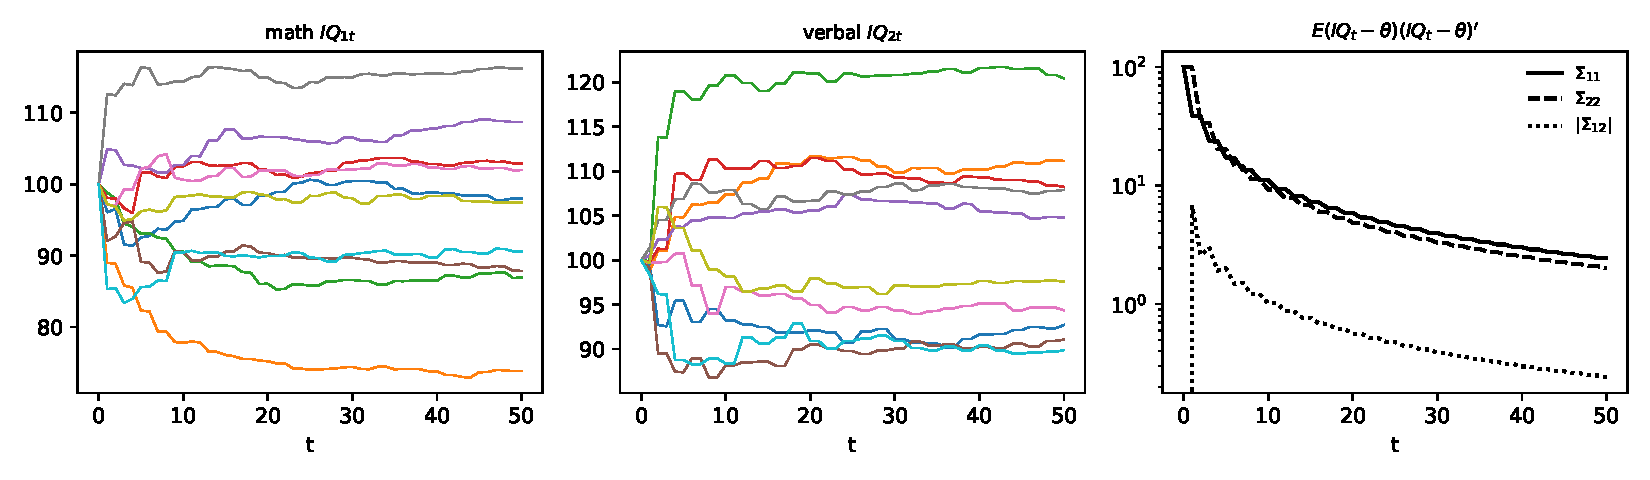
\includegraphics[width=\textwidth]{figures/ch2_26.pdf}\\
{\small Figure S2.6. Simulated math and verbal IQ paths for 10 persons and the elements of $\Sigma_t$ (log scale).}
\end{center}

\textbf{(c)}  In information (precision) form, $\Sigma_{t+1}^{-1}=\Sigma_t^{-1}+G_t'G_t/50$, so
\[
  \Sigma_t^{-1}=\frac{I}{100}+\frac1{50}\sum_{s=0}^{t-1}G_s'G_s .
\]
Every two periods the sum grows by $M=G_e'G_e+G_o'G_o=\begin{bmatrix}.8101&.0999\\.0999&.9901\end{bmatrix}$, which is positive definite because
$G_e=(.9,.1)$ and $G_o=(.01,.99)$ are linearly independent.  Hence $\lambda_{\min}(\Sigma_t^{-1})\ge\lfloor t/2\rfloor\lambda_{\min}(M)/50\to\infty$, and
$\Sigma_t\to0$.  Each test mostly measures one ability, but because the two tests load on the abilities in linearly independent ways, alternating
them identifies both.  Numerically, $\Sigma_{50}=\begin{bmatrix}2.438&-0.241\\-0.241&2.004\end{bmatrix}$, and it falls roughly like $1/t$.
\end{ex}

%%---------------------------------------------------------------------------
\begin{ex}{2.27}{A two-person consumption loans economy}
\textbf{(a)}  By \bk{(2.12.9)}, $c_t=(1-\beta)\bigl[E_t\sum_j\beta^jy_{t+j}-b_t\bigr]$.  Since $y^i$ is i.i.d.\ with mean $.75$,
$E_t\sum_j\beta^jy^i_{t+j}=y^i_t+\frac{.75\beta}{1-\beta}$, so
\[
  c^i_t=(1-\beta)(y^i_t-b^i_t)+.75\beta .
\]
The budget constraint gives $b^i_{t+1}=\beta^{-1}(c^i_t+b^i_t-y^i_t)=b^i_t+.75-y^i_t$.  For consumer 1, $y^1_t=1$ when $s_t=0$ and $.5$ when $s_t=1$,
so $b^1_{t+1}=b^1_t-.25$ or $b^1_t+.25$.  For consumer 2 the signs are reversed.  A consumer saves (reduces debt by) the
excess of current income over its mean.

\textbf{(b)}  $b^i_{t+1}-b^i_t=.75-y^i_t$ and $c^i_{t+1}-c^i_t=(1-\beta)(y^i_{t+1}-.75)$ are i.i.d.\ with mean zero, so $b^i_t$ and $c^i_t$ are random walks
(unit roots).  But $c^i_t+(1-\beta)b^i_t=(1-\beta)y^i_t+.75\beta$ is i.i.d.\ and hence stationary.  So $(c^i_t,b^i_t)$ is cointegrated with cointegrating
vector $(1,\,1-\beta)$, as in \bk{(2.12.19)}.

\textbf{(c)}  $b^i_{t+1}=b^i_t+.75-y^i_t$ is a function of $(b^i_t,s_t)$, both known at $t$.  It does not depend on $s_{t+1}$, so it is independent of news
arriving at $t+1$: the payoff of a one-period IOU is risk-free.

\textbf{(d)}  $(b^1+b^2)_{t+1}-(b^1+b^2)_t=1.5-(y^1_t+y^2_t)=0$, so $b^1_t+b^2_t=b^1_0+b^2_0=0$ for all $t$.  Then
$c^1_t+c^2_t=(1-\beta)[(y^1_t+y^2_t)-(b^1_t+b^2_t)]+1.5\beta=1.5$ (this holds from $t=0$ on).  Aggregate consumption equals the constant aggregate endowment, and
one consumer's debt is the other's asset.  The decision rules therefore describe a closed pure consumption-loans economy: in a state where $y^1$
is high, consumer 1 lends $.25$ to consumer 2 by buying a one-period IOU at price $\beta$, and the interest rate $R=\beta^{-1}$ clears the loan
market.

\textbf{(e)}  $u'(c)=\gamma-c$ and $c^i_{t+1}=c^i_t+(1-\beta)(y^i_{t+1}-.75)$, so
$m^i_{t+1}=\beta\bigl[1-\frac{(1-\beta)(y^i_{t+1}-.75)}{\gamma-c^i_t}\bigr]$.  Consumer 1 has high income ($y^1=1$) when $s_{t+1}=0$, so
\[
  m^1_{t+1}=\begin{cases}\beta-\dfrac{.25\,\beta(1-\beta)}{\gamma-c^1_t},& s_{t+1}=0,\\[2ex]\beta+\dfrac{.25\,\beta(1-\beta)}{\gamma-c^1_t},& s_{t+1}=1,\end{cases}\qquad
  m^2_{t+1}=\begin{cases}\beta+\dfrac{.25\,\beta(1-\beta)}{\gamma-c^2_t},& s_{t+1}=0,\\[2ex]\beta-\dfrac{.25\,\beta(1-\beta)}{\gamma-c^2_t},& s_{t+1}=1.\end{cases}
\]
\rmk{The book's display has the two branches of each discount factor interchanged.  In the state where a consumer's income is high,
consumption rises and marginal utility falls, so the discount factor is below $\beta$, not above.  (Also, ``$\text{Prob}(s_1=0)$'' in the statement
should read $\text{Prob}(s_t=0)$.)}
The discount factors are \emph{not} equal: in each state one is above and the other below $\beta$.  With only a risk-free bond, markets are
incomplete, and marginal rates of substitution are not equalized state by state.

\textbf{(f)}  In both cases the two branches are $\beta\pm x$ with probability $\frac12$ each, so $E_tm^1_{t+1}=E_tm^2_{t+1}=\beta=R^{-1}$.  Both consumers
agree on the price of the only traded asset, the risk-free bond, though not on the prices of state-contingent claims.
\end{ex}

%%---------------------------------------------------------------------------
\begin{ex}{2.28}{A non-invertible moving average}
\textbf{(a)}  Formally inverting $1-2L$ gives $\epsilon_t=\sum_{j\ge0}2^jy_{t-j}$, whose weights explode.  To prove that no square-summable
representation exists, let $H(y^t)$ be the closed linear span of $\{y_s,s\le t\}$ and $a_t=y_t-E[y_t\given H(y^{t-1})]$.  Since $\epsilon_t$ is
independent of $\epsilon_{t-1},\epsilon_{t-2},\dots$, it is orthogonal to $H(y^{t-1})$.  Hence its projection on $H(y^t)=H(y^{t-1})\oplus\{a_t\}$ is
\[
  E[\epsilon_t\given H(y^t)]=\frac{E\epsilon_ta_t}{Ea_t^2}\,a_t=\frac{E\epsilon_ty_t}{4}\,a_t=\frac{a_t}{4},
\]
using $Ea_t^2=4$ from (c).  Its variance is $1/4<1=\var\epsilon_t$, so $\epsilon_t\notin H(y^t)$.  Even the whole past and present of $y$ leave
$3/4$ of the variance of $\epsilon_t$ unexplained.

\textbf{(b)}  $x_t=(\epsilon_t,\epsilon_{t-1})'$, $x_{t+1}=Ax_t+Cw_{t+1}$ and $y_t=Gx_t$ with
$A=\begin{bmatrix}0&0\\1&0\end{bmatrix}$, $C=\begin{bmatrix}1\\0\end{bmatrix}$, $G=\begin{bmatrix}1&-2\end{bmatrix}$, $w_{t+1}=\epsilon_{t+1}$, and no measurement error.

\textbf{(c)}  Iterating the Kalman filter (the Python analogue of \texttt{kfilter.m}) converges to $K=(0,\,0.25)'$ and $\Omega=G\Sigma G'=4$.  The
innovations representation $\hat x_{t+1}=A\hat x_t+Ka_t$, $y_t=G\hat x_t+a_t$ has moving-average coefficients $1,\ GK=-0.5,\ GAK=0,\dots$, so
$y_t=a_t-.5a_{t-1}$.  As a check, both representations have the same autocovariances: $\gamma_0=1+4=5=1.25\cdot4$ and $\gamma_1=-2=-.5\cdot4$.  The
innovation variance is $\var(a_t)=4$, four times $\var(\epsilon_t)$.  Flipping the root from $2$ to $1/2$ makes the representation invertible, at
the cost of a larger shock variance.

\textbf{(d)}  $(1-.5L)^{-1}y_t=a_t$, i.e.\ $\sum_{j\ge0}.5^jy_{t-j}=a_t$, so
\[
  y_t=-\sum_{j\ge1}(.5)^jy_{t-j}+a_t,\qquad A_j=-(.5)^j,
\]
with $Ea_ty_{t-j}=0$ for $j\ge1$.

\textbf{(e)}  None of them.  Since $y$ is Gaussian, the distribution of $y_{t+1}$ given its past is normal with variance $4$ and mean
$-\sum_{j\ge0}.5^{j+1}y_{t-j}$, which depends on every lag (all $A_j\ne0$).  So no finite window $(y_t,\dots,y_{t-k})$ is a sufficient statistic, and none of the three vectors is Markov.

\textbf{(f)}  From $y_{t+1}=\epsilon_{t+1}-2\epsilon_t$, $\epsilon_t=\frac12(\epsilon_{t+1}-y_{t+1})$.  Iterating forward,
$\epsilon_t=-\sum_{j=1}^k2^{-j}y_{t+j}+2^{-k}\epsilon_{t+k}$, and the remainder vanishes in mean square as $k\to\infty$.  Hence
$\epsilon_t=-\sum_{j\ge1}2^{-j}y_{t+j}$, with square-summable weights.  The shock $\epsilon_t$ lies in the span of the \emph{future} of $y$, not of its past.
\end{ex}

%%---------------------------------------------------------------------------
\begin{ex}{2.29}{Pure prediction and the Lyapunov equation}
\exnote{Equation (3) refers to a numbered display of the exercise in the book.}
\textbf{(a)}  Iterating the equation forward $k$ times,
$\mu_t=\sum_{j=0}^{k-1}(A')^jRx_{t+j}+(A')^k\mu_{t+k}$.  With $A$ stable and bounded $\mu$, the remainder vanishes, so
\[
  \mu_t=\sum_{j=0}^\infty(A')^j\,R\,x_{t+j}=\Bigl(\sum_{j\ge0}(A')^jRA^j\Bigr)x_t .
\]
\rmk{The exercise writes the solution as $R\sum_j(A')^jx_{t+j}$, with $R$ in front of the sum.  That expression satisfies the equation only if $R$
commutes with $A'$: substituting it gives $Rx_t+A'R\sum_j(A')^jx_{t+1+j}$, which equals $R\sum_j(A')^jx_{t+j}$ iff $A'R=RA'$.  The correct solution puts $R$ between
$(A')^j$ and $x_{t+j}$, as above.  (The second part is also mislabelled ``a.''.)}

\textbf{(b)}  If $\mu_t=Px_t$ for all $x_t$, then $Px_t=Rx_t+A'PAx_t$, so $P=R+A'PA$.  The unique solution is $P=\sum_j(A')^jRA^j$, which converges because $A$ is stable.
This is the matrix found in (a).

\textbf{(c)}  \bk{(2.4.10)}, $\Sigma_\infty=A\Sigma_\infty A'+CC'$, is the same Lyapunov equation with $A$ replaced by $A'$ and $R$ by $CC'$:
$\Sigma_\infty=\sum_jA^jCC'(A')^j$ versus $P=\sum_j(A')^jRA^j$.  Covariances propagate forward in time through $A$, while values (shadow prices) cumulate
backward from the future through $A'$.  The two equations are duals of each other.

\textbf{(d)}  \bk{(2.4.25)}, $P_0=R+F_0'QF_0+\beta(A-BF_0)'P_0(A-BF_0)$, is (3) with $A\to\sqrt\beta(A-BF_0)$ and $R\to R+F_0'QF_0$.  Evaluating a
fixed decision rule, the policy-evaluation step of Howard's algorithm, is a pure prediction problem: summing discounted quadratic
forms along the closed-loop path.

\textbf{(e)}  Use the duality $A\leftrightarrow A'$, $B\leftrightarrow G'$, $R\leftrightarrow CC'$, $Q\leftrightarrow R_v$ (the measurement-error
covariance) and $F\leftrightarrow K'$ between the regulator and the filter.  Start from a gain $K_0$ with $A-K_0G$ stable, and iterate:
\begin{enumerate}[label=\arabic*.]
\item (evaluate) given $K_j$, solve the Lyapunov equation
$\Sigma_j=(A-K_jG)\Sigma_j(A-K_jG)'+CC'+K_jR_vK_j'$ for the estimation-error covariance obtained by using the fixed gain $K_j$ forever;
\item (improve) set $K_{j+1}=A\Sigma_jG'(G\Sigma_jG'+R_v)^{-1}$.
\end{enumerate}
This is exactly \bk{(2.4.30)} applied to the dual regulator problem (with $\beta=1$).  Like Howard's algorithm, it is a Newton method and converges
in a handful of steps.  For the model of exercise 2.24, starting from $K_0=0$, it reaches $K=0.53767$ and $\Sigma=1.48390$ in 6 iterations
(\texttt{ch2.py}), the same as iterating the Riccati equation to convergence.
\end{ex}

%%---------------------------------------------------------------------------
\begin{ex}{2.30}{Quasi-hyperbolic discounting: Phelps and Pollak meet Howard}
\textbf{(a)}  $V(x)=\sum_{j\ge0}\beta^jr(x_j,-Fx_j)$ with $x_0=x$ and $x_{j+1}=(A-BF)x_j$.  $V(x)$ is the value, discounted \emph{exponentially} at rate
$\beta$, of the return stream generated by using the rule $u=-Fx$ forever, starting from $x$.

\textbf{(b)}  Guess $V(x)=-x'Px$.  Matching quadratic forms gives the Lyapunov equation
\[
  P=R+F'QF+\beta(A-BF)'P(A-BF),
\]
i.e.\ \bk{(2.4.25)}.  It has a unique positive definite solution if $\sqrt\beta(A-BF)$ is stable.  Compute it by iterating
$P_{k+1}=R+F'QF+\beta(A-BF)'P_k(A-BF)$ from $P_0=0$, or faster with the doubling algorithm (\texttt{doublej}).

\textbf{(c)}  $U(x)$ is the value to the \emph{current} decision maker, who gives weight 1 to today and $\delta\beta^j$ to date $t+j$, when he chooses today's
action optimally, taking as given that all future decision makers use $u=-Fx$.  The first-order condition gives
$G=\delta\beta(Q+\delta\beta B'PB)^{-1}B'PA$.

\textbf{(d)}  A (stationary linear) Markov perfect equilibrium is a rule $F$ such that, if all future decision makers use $u=-Fx$, the current
decision maker's best response is also $u=-Fx$: $G(F)=F$.  Equivalently, a pair $(F,P)$ with
\[
  P=R+F'QF+\beta(A-BF)'P(A-BF),\qquad F=\delta\beta(Q+\delta\beta B'PB)^{-1}B'PA .
\]

\textbf{(e)}  Iterate on best responses: given $F_j$, solve the Lyapunov equation for $P_j$, set $F_{j+1}=\delta\beta(Q+\delta\beta B'P_jB)^{-1}B'P_jA$, and repeat
to convergence.  (Convergence is not guaranteed in general, but the iteration converges quickly in examples; see below.)

\textbf{(f)}  With $\delta=1$ this is exactly Howard's policy improvement algorithm \bk{(2.4.30)}.  With $\delta<1$ the evaluation step discounts at
$\beta$ but the improvement step discounts at $\delta\beta$.  The fixed point is then an equilibrium of a game among the successive selves, not the
maximum of any single objective, and the monotone-improvement property of Howard's algorithm is lost.

\textbf{(g)}  Yes.  The equilibrium strategy is stationary and depends only on the current state, and the conditions defining it are the same at every
date.  So the continuation from any date and state is again a Markov perfect equilibrium (it is subgame perfect).

\textbf{(h)}  From date 1 on, the dictator's weights $\delta\beta,\delta\beta^2,\dots$ are proportional to $1,\beta,\beta^2,\dots$.  So the continuation is a standard
exponential-discounting LQ problem, with value $W(x)=-x'P^*x$ solving the Riccati equation
\[
  P^*=R+\beta A'P^*A-\beta^2A'P^*B(Q+\beta B'P^*B)^{-1}B'P^*A,
\]
\[
  u_t=-F^*x_t\ \ (t\ge1),\qquad F^*=\beta(Q+\beta B'P^*B)^{-1}B'P^*A .
\]
At date 0, $\max_u\{r(x_0,u)+\delta\beta W(Ax_0+Bu)\}$ gives
\[
  u_0=-G^*x_0,\qquad G^*=\delta\beta(Q+\delta\beta B'P^*B)^{-1}B'P^*A .
\]
The dictator's plan is $u_0=-G^*x_0$, then $u_t=-F^*x_t$.

\textbf{(i)}  No, unless $\delta=1$.  The time-1 dictator weights date 1 by $1$ and later dates by $\delta\beta^j$, so she would choose $u_1=-G^*x_1$ rather than
the $u_1=-F^*x_1$ planned at date 0.  The preferences are time inconsistent.

\textbf{(j)}  With $\delta=1$: then $G^*=F^*$, the dictator's plan is time consistent, and the Markov perfect equilibrium coincides with the optimal
exponential-discounting rule $F^*$.  For $\delta<1$ they differ generically.  An example (\texttt{ch2.py}) with
$A=\begin{bmatrix}1&.1\\0&.9\end{bmatrix}$, $B=(0,1)'$, $R=I$, $Q=1$, $\beta=.95$ gives:
\begin{center}
\begin{tabular}{lccc}
\toprule
 & MPE $F$ & dictator, date 0: $G^*$ & dictator, dates $\ge1$: $F^*$\\
\midrule
$\delta=1$ & $(0.4562,\,0.5965)$ & $(0.4562,\,0.5965)$ & $(0.4562,\,0.5965)$\\
$\delta=.7$ & $(0.3938,\,0.5146)$ & $(0.3912,\,0.5114)$ & $(0.4562,\,0.5965)$\\
\bottomrule
\end{tabular}
\end{center}
(The MPE iteration converged in 7 and 14 steps.)  With present bias ($\delta<1$), each self acts less aggressively than the exponential discounter
would, and the equilibrium rule is not the continuation of anyone's optimal plan.
\end{ex}

%% ===========================================================================
%% Chapter 3. Dynamic Programming
%% ===========================================================================
\solchapter{3}{Dynamic Programming}

\begin{center}
\begin{minipage}{0.86\textwidth}
\small
Solution to the single exercise of Chapter 3 of Ljungqvist and Sargent, \emph{Recursive Macroeconomic Theory} (4th edition, 2018).
\end{minipage}
\end{center}

\bigskip
\hrule
\bigskip

%%---------------------------------------------------------------------------
\begin{ex}{3.1}{Howard's policy iteration algorithm}
Write $y_t=Ak_t^\alpha\theta_t$ for output and $z_t=\ln y_t$.

\emph{Step 1: evaluating an arbitrary policy.}  Under $k_{t+1}=hy_t$ with $h\in(0,1)$, consumption is $c_t=(1-h)y_t>0$ and
\[
  z_{t+1}=\ln A+\alpha\ln k_{t+1}+\ln\theta_{t+1}=\ln A+\alpha\ln h+\alpha z_t+\ln\theta_{t+1}.
\]
Since $E\ln\theta=0$, $E_0z_t=\alpha^tz_0+(\ln A+\alpha\ln h)\frac{1-\alpha^t}{1-\alpha}$.  Therefore
\begin{align*}
  J_h(k_0,\theta_0)&=\sum_{t\ge0}\beta^t\bigl[\ln(1-h)+E_0z_t\bigr]
  =\frac{\ln(1-h)}{1-\beta}+\frac{z_0}{1-\alpha\beta}+\frac{\ln A+\alpha\ln h}{1-\alpha}\Bigl(\frac1{1-\beta}-\frac1{1-\alpha\beta}\Bigr)\\
  &=\underbrace{\frac{\ln(1-h)}{1-\beta}+\frac{\beta(\ln A+\alpha\ln h)}{(1-\beta)(1-\alpha\beta)}+\frac{\ln A}{1-\alpha\beta}}_{\equiv\;\kappa(h)}
  +\frac{\alpha}{1-\alpha\beta}\ln k_0+\frac1{1-\alpha\beta}\ln\theta_0 .
\end{align*}
The key fact is that the policy parameter $h$ affects only the constant $\kappa(h)$.  The coefficient on $\ln k$, $\alpha/(1-\alpha\beta)$, is the same for every $h$,
because under any constant-savings-rate policy the elasticity of future output with respect to current capital is $\alpha^t$.

\emph{Step 2: the improvement step.}  With $J_0=J_{h_0}$,
$EJ_0(k',\theta')=\kappa(h_0)+\frac{\alpha}{1-\alpha\beta}\ln k'$ (using $E\ln\theta'=0$), so the improvement problem is
\[
  \max_{k'}\Bigl\{\ln(y-k')+\frac{\alpha\beta}{1-\alpha\beta}\ln k'\Bigr\}+\text{constant}.
\]
The objective is strictly concave, and the first-order condition $\frac1{y-k'}=\frac{\alpha\beta}{1-\alpha\beta}\cdot\frac1{k'}$ gives $k'=\alpha\beta\,y$.  Hence
\[
  h_1=\alpha\beta\qquad\text{for every initial guess }h_0\in(0,1).
\]

\emph{Step 3: convergence and optimality.}  Repeating the improvement step from $J_1=J_{\alpha\beta}$ again gives $h_2=\alpha\beta$, because the coefficient on $\ln k'$ is the same.  So the
iterations have converged after one step.  The limit is optimal: $J_{\alpha\beta}$ satisfies the Bellman equation
$J(k,\theta)=\max_{k'}\{\ln(Ak^\alpha\theta-k')+\beta EJ(k',\theta')\}$, since the maximum is attained at $k'=\alpha\beta Ak^\alpha\theta$, the policy that generates
$J_{\alpha\beta}$.  It coincides with the solution obtained by guess and verify in section \bk{3.1.2}, $k_{t+1}=\alpha\beta Ak_t^\alpha\theta_t$, extended to the
multiplicative shock.  (The unbounded log return does not cause trouble here: along any constant-savings policy the value is finite, and the
guess-and-verify argument of section \bk{3.1.2} delivers the same function.)

\emph{Why one step?}  Policy iteration is Newton's method on the Bellman equation.  In this model the Bellman equation is ``linear'' in
the right coordinates: every constant-savings-rate policy produces a value function in the same two-parameter family (affine in $\ln k$ and $\ln\theta$),
with the payoff-relevant slope already correct.  So a single Newton step lands on the fixed point.
\end{ex}

%% ===========================================================================
%% Chapter 5. Linear Quadratic Dynamic Programming
%% ===========================================================================
\solchapter{5}{Linear Quadratic Dynamic Programming}

\begin{center}
\begin{minipage}{0.86\textwidth}
\small
Solutions to all 14 exercises of Chapter 5 of Ljungqvist and Sargent, \emph{Recursive Macroeconomic Theory} (4th edition, 2018).
The Matlab programs the exercises refer to (\texttt{olrp.m}, \texttt{policyi.m}, \texttt{doublej.m}, \texttt{dlqrmon.m}) are replaced by the Python
functions \texttt{olrp}, \texttt{lq\_howard} and \texttt{doublej} in \texttt{code/rmtlib.py}; all numbers come from \texttt{code/ch5.py}.
\end{minipage}
\end{center}

\bigskip
\hrule
\bigskip

Conventions: a linear regulator \emph{minimizes} $\sum_t\beta^t(x_t'Rx_t+u_t'Qu_t+2u_t'Hx_t)$ subject to $x_{t+1}=Ax_t+Bu_t\,(+Cw_{t+1})$.  The
value of the corresponding maximization problem is $v(x)=-x'Px\,(-d)$, and the optimal rule is $u_t=-Fx_t$.

%%---------------------------------------------------------------------------
\begin{ex}{5.1}{A regulator with cross products}
\textbf{(a)}  Guess $v(x)=-x'Px$ with $P$ symmetric.  The Bellman equation is
\[
  -x'Px=\max_u-\bigl\{x'Rx+u'Qu+2u'Hx+\beta(Ax+Bu)'P(Ax+Bu)\bigr\}.
\]
Collect terms: the braces equal $x'(R+\beta A'PA)x+u'Mu+2u'Nx$ with $M=Q+\beta B'PB$ and $N=\beta B'PA+H$.  $M$ is positive definite (as $Q$ is and $P\succeq0$), so the
objective is strictly concave in $u$.  The first-order condition $Mu+Nx=0$ gives
\[
  u=-M^{-1}Nx=-(Q+\beta B'PB)^{-1}(\beta B'PA+H)\,x .
\]
At the optimum, $u'Mu+2u'Nx=x'N'M^{-1}Nx-2x'N'M^{-1}Nx=-x'N'M^{-1}Nx$.  Matching quadratic forms then gives
\[
  P=R+\beta A'PA-(\beta A'PB+H')(Q+\beta B'PB)^{-1}(\beta B'PA+H).
\]
Equivalently, the change of variables $u^*=u+Q^{-1}Hx$ removes the cross product: it turns the problem into a standard regulator with
$\tilde R=R-H'Q^{-1}H$, $\tilde A=A-BQ^{-1}H$, and then $F=\tilde F+Q^{-1}H$.

\textbf{(b)}  \texttt{olrp(beta, A, B, Q, R, H)} in \texttt{code/rmtlib.py} iterates
$P_{j+1}=R+\beta A'P_jA-(\beta A'P_jB+H')(Q+\beta B'P_jB)^{-1}(\beta B'P_jA+H)$ from $P_0=0$ until successive iterates differ by less than
$10^{-12}$ (relative), and returns $F=(Q+\beta B'PB)^{-1}(\beta B'PA+H)$.  On a random $3\times3$ test problem it converges in 16 iterations, with a
Riccati residual of $3\times10^{-13}$.  It reproduces the transformed problem's solution to machine precision ($|P-\tilde P|<10^{-15}$,
$|F-(\tilde F+Q^{-1}H)|<10^{-16}$).
\end{ex}

%%---------------------------------------------------------------------------
\begin{ex}{5.2}{Policy improvement for the linear regulator}
The algorithm alternates between evaluating a policy and improving it.

\emph{Evaluation.}  The value of using $u=-F_jx$ forever is $v_j(x)=-\sum_t\beta^tx_t'(R+F_j'QF_j)x_t$ with $x_{t+1}=(A-BF_j)x_t$.  It satisfies
$v_j(x)=-x'(R+F_j'QF_j)x+\beta v_j((A-BF_j)x)$.  With $v_j(x)=-x'P_jx$ this is exactly \bk{(5.2.10)}:
\[
  P_j=R+F_j'QF_j+\beta(A-BF_j)'P_j(A-BF_j),
\]
a Lyapunov equation with solution $P_j=\sum_k\beta^k(A-BF_j)'^k(R+F_j'QF_j)(A-BF_j)^k$.  It exists when the eigenvalues of $A-BF_j$ are below $\beta^{-1/2}$ in modulus.

\emph{Improvement.}  $F_{j+1}$ solves the one-period problem $\max_u\{-x'Rx-u'Qu+\beta v_j(Ax+Bu)\}$, whose first-order condition
$(Q+\beta B'P_jB)u=-\beta B'P_jAx$ is \bk{(5.2.11)}: $F_{j+1}=\beta(Q+\beta B'P_jB)^{-1}B'P_jA$.

\emph{Why it improves.}  Let $T_Fv(x)=-x'(R+F'QF)x+\beta v((A-BF)x)$ and $Tv=\max_FT_Fv$.  Both operators are monotone.  By construction
$T_{F_{j+1}}v_j=Tv_j\ge T_{F_j}v_j=v_j$.  Applying $T_{F_{j+1}}$ repeatedly and using monotonicity gives $v_{j+1}=\lim_kT^k_{F_{j+1}}v_j\ge v_j$, i.e.\
$P_{j+1}\preceq P_j$.  The value never deteriorates, and every rule the algorithm visits keeps $\sqrt\beta(A-BF_j)$ stable.

\emph{Fixed point.}  If $F_{j+1}=F_j=F$, then $(Q+\beta B'PB)F=\beta B'PA$.  Expanding \bk{(5.2.10)},
\[
  P=R+\beta A'PA-\beta(A'PBF+F'B'PA)+F'(Q+\beta B'PB)F=R+\beta A'PA-\beta F'B'PA,
\]
because $F'(Q+\beta B'PB)F=\beta F'B'PA$ and $A'PBF=(F'B'PA)'=F'B'PA$ (a symmetric matrix).  Substituting $F$ gives
$P=R+\beta A'PA-\beta^2A'PB(Q+\beta B'PB)^{-1}B'PA$, the algebraic Riccati equation of the discounted problem.  So the limit of the policy
improvement algorithm is the optimal rule.
\end{ex}

%%---------------------------------------------------------------------------
\begin{ex}{5.3}{A household's saving problem}
\textbf{(a)}  State $x_t=(a_t,y_t,y_{t-1},1)'$ and control $u_t=i_t$.  Then $c_t-b=h'x_t-u_t$ with $h=(r,1,0,-b)'$, so
$(c_t-b)^2+\gamma i_t^2=x_t'hh'x_t-2u_th'x_t+(1+\gamma)u_t^2$.  Hence
\[
  R=hh',\quad Q=1+\gamma,\quad H=-h',\qquad
  A=\begin{bmatrix}1&0&0&0\\0&\rho_1&\rho_2&0\\0&1&0&0\\0&0&0&1\end{bmatrix},\quad B=\begin{bmatrix}1\\0\\0\\0\end{bmatrix}.
\]

\textbf{(b)}  \texttt{olrp} converges in 496 iterations; Howard's algorithm gives the same $F$ to $3\times10^{-10}$.  The optimal rules are
\[
  i_t=0.316713\,y_t+0.055891\,y_{t-1},\qquad c_t=ra_t+y_t-i_t=0.052632\,a_t+0.683287\,y_t-0.055891\,y_{t-1}.
\]
Three features stand out.
\begin{itemize}[leftmargin=*]
\item The bliss level $b=30$ does not appear.  With $\beta(1+r)=1$, a constant consumption gap $c-b$ satisfies the Euler equation: the marginal cost
$b-c$ of saving a unit today equals the discounted value $r\sum_{s\ge1}\beta^s(b-c)$ of the extra consumption it finances forever.  So the level of $b$
cannot affect saving.
\item The household consumes exactly the interest on its assets, $ra_t$, and never draws down wealth: investment does not depend on $a_t$.
\item Assets therefore follow a unit-root process: the closed-loop matrix $A-BF$ has eigenvalues $0.355,\,0.845$ (those of the income process), $1$
(assets) and $1$ (the constant).  Because income is transitory here (it decays to zero), the household saves a large share, $31.7\%$, of current income.
\end{itemize}
\end{ex}

%%---------------------------------------------------------------------------
\begin{ex}{5.4}{Durable goods and habits}
\textbf{(a)}  State $x_t=(a_t,y_t,y_{t-1},h_t,1)'$, control $u_t=i_t$.  With $c_t=ra_t+y_t-u_t$,
$s_t-b=\tilde h'x_t-\pi u_t$ where $\tilde h=(\pi r,\pi,0,\lambda,-b)'$.  So
\[
  R=\tilde h\tilde h',\quad Q=\pi^2+\gamma,\quad H=-\pi\tilde h',\qquad
  A=\begin{bmatrix}1&0&0&0&0\\0&\rho_1&\rho_2&0&0\\0&1&0&0&0\\\theta r&\theta&0&\delta&0\\0&0&0&0&1\end{bmatrix},\quad
  B=\begin{bmatrix}1\\0\\0\\-\theta\\0\end{bmatrix}.
\]

\textbf{(b), (c)}  The Riccati iteration and Howard's algorithm agree to $4\times10^{-10}$.  Writing both rules in terms of $x_t=(a_t,y_t,y_{t-1},h_t)$ (the
constant has a zero coefficient again, for the reason given in exercise 5.3):
\begin{center}
\begin{tabular}{lccccc}
\toprule
 & & $a_t$ & $y_t$ & $y_{t-1}$ & $h_t$\\
\midrule
(b) durables & $i_t$ & $-0.2991$ & $-1.5205$ & $0.6121$ & $0.2842$\\
 & $c_t$ & $0.3517$ & $2.5205$ & $-0.6121$ & $-0.2842$\\
\addlinespace
(c) habits & $i_t$ & $-0.1792$ & $-0.6881$ & $0.4254$ & $0.1702$\\
 & $c_t$ & $0.2318$ & $1.6881$ & $-0.4254$ & $-0.1702$\\
\addlinespace
exercise 5.3 & $c_t$ & $0.0526$ & $0.6833$ & $-0.0559$ & ---\\
\bottomrule
\end{tabular}
\end{center}
The closed-loop eigenvalues are $\{0.355,0.367,0.845,1,1\}$ in (b) and $\{0.355,0.601,0.845,1,1\}$ in (c).

\textbf{(d)}  \emph{Durables} ($\lambda=1$, small $\pi$, $\delta=.95$, $\theta=1$): utility comes almost entirely from the stock $h_t$ of durables, which depreciates at 5\% and
is replenished by purchases $c_t$.  The household smooths services $s_t$, not purchases.  A rise in income raises the desired stock, and since
purchases are the only way to adjust the stock, expenditures jump far more than one for one: the coefficient on $y_t$ is $2.52$, versus $0.68$ for
nondurable consumption in exercise 5.3.  The household dissaves ($i_t<0$) to finance the purchase.  A larger existing stock $h_t$ reduces
purchases.  This is the familiar excess volatility of durable expenditures, an accelerator.

\emph{Habits} ($\lambda=-1$, $\pi=1$): services are $s_t=c_t-h_t$, where the habit stock $h_t$ accumulates past consumption.  Consumption today raises
utility today but also raises the habit, which lowers future services.  The household internalizes this cost: consumption again
responds to income more than in the model without habits, and it falls with the habit stock.  Note that with $\delta=.95$, $\theta=1$ the habit stock is
twenty times consumption in a steady state, so $s=c-h=-19c$.  Bliss $s=b=30$ would require negative consumption.  That is allowed in this LQ
setting, but it shows these particular parameters are not a realistic habit specification (a small $\theta$, such as $.05$, would be).
\end{ex}

%%---------------------------------------------------------------------------
\begin{ex}{5.5}{A geometric sum of forecasts}
\textbf{(a)}  With $x_t=(y_t,y_{t-1},w_t)'$, $x_{t+1}=Ax_t+Cw_{t+1}$ where $A=\begin{bmatrix}\rho_1&\rho_2&\gamma\\1&0&0\\0&0&0\end{bmatrix}$ and $C=(1,0,1)'$.  With $y_t=Gx_t$, $G=(1,0,0)$,
\bk{(2.4.18)} gives $E_t\sum_j\beta^jy_{t+j}=G(I-\beta A)^{-1}x_t$ (valid since the eigenvalues of $\beta A$ are inside the unit circle).  Solving
$v(I-\beta A)=G$ for the row vector $v$ gives a closed form:
\[
  E\Bigl[\sum_{j\ge0}\beta^jy_{t+j}\Bigm|y^t,w^t\Bigr]=\frac{y_t+\beta\rho_2y_{t-1}+\beta\gamma w_t}{1-\beta\rho_1-\beta^2\rho_2}.
\]

\textbf{(b)}  $1-\beta\rho_1-\beta^2\rho_2=1-1.14+.361=0.221$, so
\[
  E_t\sum_j\beta^jy_{t+j}=4.52489\,y_t-1.71946\,y_{t-1}+2.14932\,w_t .
\]
\texttt{ch5.py} confirms this by summing the forecasts $GA^jx$ directly.
\end{ex}

%%---------------------------------------------------------------------------
\begin{ex}{5.6}{Finding the state is an art}
\textbf{(a)}  The summand $s_td_t=\beta^t(b_0d_t-b_1d_t^2)$ is a quadratic form in the state $x_t=(d_t,d_{t-1},1)'$:
\[
  x_{t+1}=\underbrace{\begin{bmatrix}\rho_1&\rho_2&\rho_0\\1&0&0\\0&0&1\end{bmatrix}}_{A}x_t+\underbrace{\begin{bmatrix}\sigma_d\\0\\0\end{bmatrix}}_{C}\epsilon_{t+1},\qquad
  b_0d_t-b_1d_t^2=x_t'Yx_t,\quad Y=\begin{bmatrix}-b_1&0&b_0/2\\0&0&0\\b_0/2&0&0\end{bmatrix}.
\]
By \bk{(2.4.19)}--\bk{(2.4.20)}, $v_0=x_0'\nu x_0+\sigma$, where
\[
  \nu=Y+\beta A'\nu A,\qquad \sigma=\frac{\beta}{1-\beta}\tr(\nu CC').
\]
Algorithm: (1) solve the Lyapunov equation for $\nu$, either by iterating $\nu_{k+1}=Y+\beta A'\nu_kA$ from $\nu_0=0$ or with the doubling algorithm
($\nu_{k+1}=\nu_k+\beta^{2^k}A_k'\nu_kA_k$, $A_{k+1}=A_k^2$); (2) compute $\sigma$; (3) evaluate at $x_0=(d_0,d_{-1},1)'$.  The same $\nu,\sigma$ give the value $v_t=x_t'\nu x_t+\sigma$ at
every date, because the problem is time invariant.  (Recursively, $v_t\equiv E_t\sum_{j\ge0}\beta^j(b_0-b_1d_{t+j})d_{t+j}$ satisfies $v_t=(b_0-b_1d_t)d_t+\beta E_tv_{t+1}$.)

\textbf{(b)}  The series defining $\nu$ is $\sum_k\beta^kA'^kYA^k$, which converges if every eigenvalue of $\sqrt\beta A$ lies inside the unit circle.  The
eigenvalues of $A$ are $1$ (the constant, harmless since $\sqrt\beta<1$) and the roots $\lambda_1,\lambda_2$ of $\lambda^2-\rho_1\lambda-\rho_2=0$.  So a sufficient condition
is
\[
  |\lambda_i|<\beta^{-1/2},\quad i=1,2 .
\]
It is needed because $E_0d_t^2$ grows like $|\lambda_{\max}|^{2t}$, so $\beta^tE_0d_t^2\to0$ requires $\beta|\lambda_{\max}|^2<1$ (it then also covers the linear term,
$\beta|\lambda_{\max}|<1$).  A simple sufficient condition on the coefficients is $|\rho_1|+|\rho_2|<\beta^{-1/2}$, because $|\lambda|\ge1$ with $|\lambda|^2=|\rho_1\lambda+\rho_2|$ would require
$|\lambda|\le|\rho_1|+|\rho_2|$.  In particular, $d$ may even have a unit root: $\beta<1$ still makes the sums converge.
\end{ex}

%%---------------------------------------------------------------------------
\begin{ex}{5.7}{Dynamic Laffer curves}
\textbf{(a)}  \emph{Approach.}  Eliminate $M$: the demand equation gives $M_t=\gamma_1p_t-\gamma_2p_{t+1}$, and the budget constraint gives $M_t=M_{t-1}+gp_t$.  Hence
\[
  \gamma_2p_{t+1}=(\gamma_1+\gamma_2-g)\,p_t-\gamma_1p_{t-1}\quad(t\ge1),\qquad p_1=\frac{(\gamma_1-g)\,p_0-M_{-1}}{\gamma_2}\quad(t=0).
\]
This is a second-order linear difference equation, so any $p_0$ determines the whole path, with $M_t=\gamma_1p_t-\gamma_2p_{t+1}$.  The program
(\texttt{ch5.py}, function \texttt{path}) iterates this recursion and checks positivity.  Its characteristic polynomial,
$\gamma_2\lambda^2-(\gamma_1+\gamma_2-g)\lambda+\gamma_1=0$, is exactly the condition for a constant gross inflation rate $\pi$ to be a stationary equilibrium,
$g=(\gamma_1-\gamma_2\pi)(1-1/\pi)$.  With $g=.05$ its roots are
\[
  \lambda_L=1.001002,\qquad \lambda_H=1.997998 .
\]
The general solution is $p_t=c_L\lambda_L^t+c_H\lambda_H^t$, where $(c_L,c_H)$ are determined by $p_0$ and $p_1(p_0)$.

\textbf{(b)}  Positivity of $M_t$ requires $p_{t+1}/p_t<\gamma_1/\gamma_2=2$.  Positivity of $p_t$ requires $c_H\ge0$: otherwise the dominant root $\lambda_H$ eventually drives
$p_t$ negative.  Now $c_H=(p_1-\lambda_Lp_0)/(\lambda_H-\lambda_L)$, so $c_H\ge0$ iff $(\gamma_1-g-\gamma_2\lambda_L)p_0\ge M_{-1}$, i.e.
\[
  p_0\ge p_0^{\min}=\frac{M_{-1}}{\gamma_1-g-\gamma_2\lambda_L}=2.004012 .
\]
For every $p_0\ge p_0^{\min}$ the path is an equilibrium.  Gross inflation $p_{t+1}/p_t$ is a weighted average of $\lambda_L$ and $\lambda_H$ that moves monotonically toward
$\lambda_H<2$, and $\pi_1=(\gamma_1-g-M_{-1}/p_0)/\gamma_2<1.999$, so $M_t>0$ throughout.  So there is a continuum of equilibria indexed by
$p_0\in[2.004012,\infty)$.  Numerically, $p_0=p_0^{\min}(1-10^{-6})$ already produces a negative price within 80 periods.

\textbf{(c)}  For $p_0>p_0^{\min}$, $c_H>0$, so $p_{t+1}/p_t\to\lambda_H$.  Since $M_t=\gamma_1p_t-\gamma_2p_{t+1}\approx c_H(\gamma_1-\gamma_2\lambda_H)\lambda_H^t$, the money growth rate also
converges to $\lambda_H$.  Both converge to $\lambda_H=1.997998$, i.e.\ almost 100\% inflation per period (Figure S5.1, left).

\textbf{(d)}  The minimal-price equilibrium has $c_H=0$: $p_t=p_0^{\min}\lambda_L^t$ from the start, and inflation and money growth are constant at
$\lambda_L=1.001002$ (0.1\% per period).  It is the unique equilibrium whose inflation does not converge to $\lambda_H$.  (The exercise's
lettering is slightly off: part (b) computes $p_0^{\min}$, and the two inflation rates are those of parts (c) and (d).)
\begin{center}
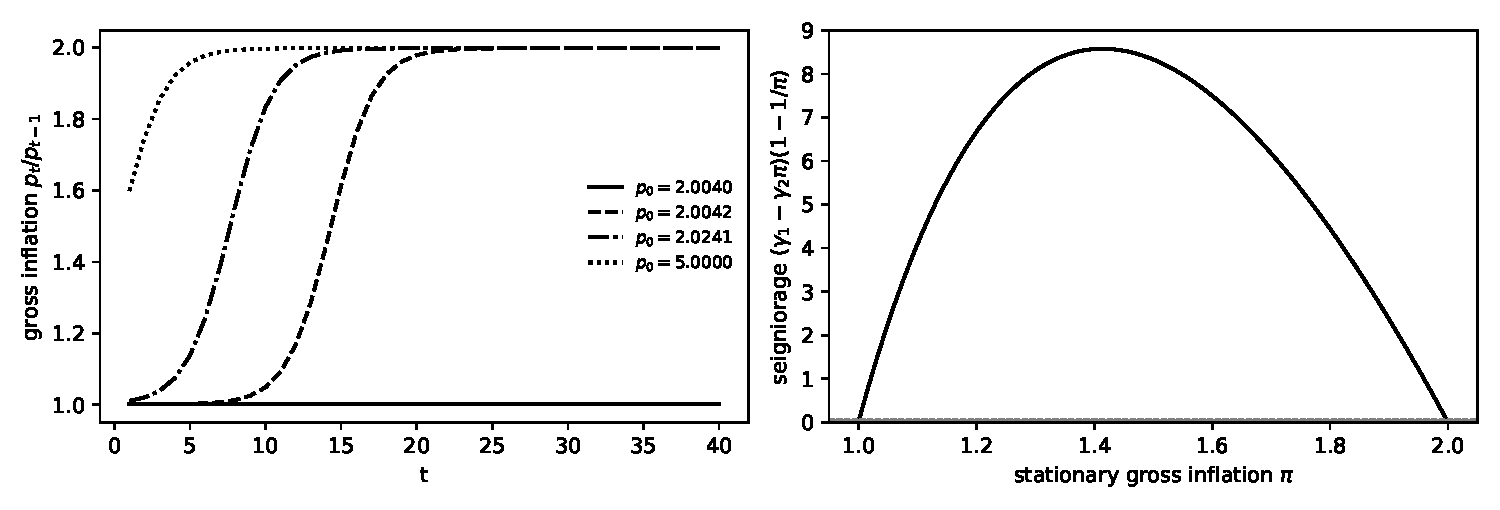
\includegraphics[width=\textwidth]{figures/ch5_07.pdf}\\
{\small Figure S5.1.  Left: gross inflation along four equilibria ($g=.05$).  Right: stationary seigniorage $(\gamma_1-\gamma_2\pi)(1-1/\pi)$; the deficits $g=.05$ and $.075$
are the nearly invisible horizontal lines near zero.}
\end{center}

\textbf{(e)}  With $g=.075$ the roots are $\lambda_L=1.001505$ and $\lambda_H=1.996995$, and $p_0^{\min}=2.006027$.  The larger deficit \emph{raises} the low stationary
inflation rate ($1.001002\to1.001505$), consistent with the view that larger deficits cause more inflation.  But it \emph{lowers} the high
rate ($1.997998\to1.996995$), toward which all other equilibria converge.  Along those equilibria, larger deficits mean lower eventual inflation.

\textbf{(f)}  Stationary seigniorage $S(\pi)=(\gamma_1-\gamma_2\pi)(1-1/\pi)$ is a Laffer curve: zero at $\pi=1$ (no inflation tax) and at $\pi=\gamma_1/\gamma_2=2$ (no money demand),
with a maximum at $\pi^*=\sqrt{\gamma_1/\gamma_2}=\sqrt2$, where $S(\pi^*)=(\sqrt{\gamma_1}-\sqrt{\gamma_2})^2=8.579$.  Any deficit $g<8.579$ can be financed at two stationary inflation rates, one on
each side of the peak.  Raising $g$ moves the low-inflation root up (the ``good'' side, where a higher tax rate raises revenue) and the high-inflation root down (the
``wrong'' side of the Laffer curve).  The continuum of equilibria converging to $\lambda_H$ lives on the wrong side: there, a
larger deficit is financed with a smaller inflation tax rate and a larger tax base.  These are the ``perverse'' comparative statics familiar from the literature on
deficits financed by seigniorage (e.g.\ Sargent and Wallace, 1981; Marcet and Sargent, 1989).
\end{ex}

%%---------------------------------------------------------------------------
\begin{ex}{5.8}{Optimal tax smoothing and what a VAR can reveal}
Here $b_t$ is the government's holding of one-period loans (assets) maturing at $t$.  The budget constraint says $T_t+b_t=g_t+qb_{t+1}$.

\textbf{(a)}  \emph{State} $x_t=(b_t,g_{Pt},g_{Tt},1)'$ (the constant carries $\mu_T$ and the linear term $w_1T$).  \emph{Control} $u_t=T_t$.  The transition law is
\[
  x_{t+1}=\underbrace{\begin{bmatrix}q^{-1}&-q^{-1}&-q^{-1}&0\\0&1&0&0\\0&0&\rho&(1-\rho)\mu_T\\0&0&0&1\end{bmatrix}}_{A}x_t
  +\underbrace{\begin{bmatrix}q^{-1}\\0\\0\\0\end{bmatrix}}_{B}T_t+\underbrace{\begin{bmatrix}0&0\\c_1&0\\0&c_2\\0&0\end{bmatrix}}_{C}\epsilon_{t+1},
\]
and the Bellman equation is
\[
  V(x)=\min_T\bigl\{w_1T+.5w_2T^2+\beta EV(Ax+BT+C\epsilon')\bigr\}.
\]
This is a stochastic linear regulator with $R=0$, $Q=.5w_2$ and cross-product term $H=(0,0,0,.5w_1)$.  The value function is quadratic, $V(x)=x'Px+d$ with
$d=\frac\beta{1-\beta}\tr(PCC')$, and the decision rule is linear, $T_t=-Fx_t$ (certainty equivalence: $F$ does not depend on $c_1,c_2$).

\emph{Computational strategy, and a pitfall.}  Because $R=0$, iterating the Riccati equation from $P=0$ converges immediately to $P\approx0$ and the rule
$T_t=-w_1/w_2$: tax at the loss-minimizing level forever and borrow without limit.  That violates the no-Ponzi condition.  The terminal
condition selects the \emph{stabilizing} solution, for which $\sqrt\beta(A-BF)$ is stable.  It can be computed by Howard's algorithm started from a
rule that keeps assets from exploding, such as $T_t=g_t-(1-q)b_t$ (which keeps $b_t$ constant), or by the invariant-subspace method of section \bk{5.5}.

\emph{Closed form when $\beta=q$.}  The Euler equation $W'(T_t)=\frac\beta qE_tW'(T_{t+1})$ becomes $E_tT_{t+1}=T_t$: taxes are a martingale (Barro's tax
smoothing).  Combining this with the present-value budget constraint $E_t\sum_jq^jT_{t+j}=E_t\sum_jq^jg_{t+j}-b_t$ gives
\[
  T_t=(1-q)\Bigl[E_t\sum_{j\ge0}q^jg_{t+j}-b_t\Bigr]=g_{Pt}+\frac{1-q}{1-q\rho}g_{Tt}+\Bigl(1-\frac{1-q}{1-q\rho}\Bigr)\mu_T-(1-q)b_t .
\]
With $\beta=q=.95$, $\rho=.8$, $\mu_T=1$, Howard's algorithm converges in two steps to exactly
$T_t=-0.05\,b_t+g_{Pt}+0.2083\,g_{Tt}+0.7917$, for any $(w_1,w_2)$.  If $\beta\ne q$, taxes drift ($E_tT_{t+1}=\frac q\beta T_t+\frac{w_1}{w_2}(\frac q\beta-1)$), and $w_1/w_2$ enters
the constant of the rule but not its slopes.  (Numerically, with $\beta=.96$ the slopes are the same for $(w_1,w_2)=(1,2)$ and $(3,5)$, and the constants are
$1.047$ versus $1.067$.)

\textbf{(b)}  With $T_t=-Fx_t$, the closed-loop system is $x_{t+1}=(A-BF)x_t+C\epsilon_{t+1}$, and $(g_{Tt},g_{Pt},T_t,b_{t+1})=Sx_t$ for a selection-and-rule matrix $S$
(rows $e_3'$, $e_2'$, $-F$, and the first row of $A-BF$).  When $\beta=q$,
\[
  T_{t+1}-T_t=c_1\epsilon_{1,t+1}+\frac{1-q}{1-q\rho}\,c_2\epsilon_{2,t+1},\qquad
  b_{t+1}=b_t+q^{-1}\Bigl[\bigl(\tfrac{1-q}{1-q\rho}-1\bigr)(g_{Tt}-\mu_T)\Bigr].
\]
Taxes are a random walk.  A permanent spending shock is taxed one for one immediately, while only the annuity value of a transitory shock is
taxed and the rest is financed by running down assets.  Assets are a unit-root process driven by the transitory component.  This is exactly the permanent
income model of section \bk{2.12} with taxes in place of consumption.

\textbf{(c)}  Let $y_t=(g_t,T_t)'$.  The model implies a state-space system $x_{t+1}=A^ox_t+C\epsilon_{t+1}$, $y_t=G^ox_t$, with $A^o=A-BF$ and
$G^o=\begin{bmatrix}0&1&1&0\\&-F&&\end{bmatrix}$.  The population VAR is the infinite-order projection
\[
  y_t=\sum_{j\ge1}\mathcal A_jy_{t-j}+a_t,\qquad Ea_ty_{t-j}'=0\ (j\ge1),
\]
obtained from the steady-state Kalman filter for this system as in \bk{(2.9.3)}: $\mathcal A_j=G^o(A^o-KG^o)^{j-1}K$ with $Ea_ta_t'=G^o\Sigma G^{o\prime}$.

\textbf{(d)}  The VAR is a function of $(A^o,C,G^o)$ only.  The exogenous parameters $\rho,c_1,c_2,\mu_T$ enter $A$ and $C$ directly.  $q$ and $\beta$ enter
through the budget constraint and the rule $F$.  Because of certainty equivalence and the linear-quadratic structure, $w_1$ and $w_2$ enter only through the
constant of $F$, and only via $w_1/w_2$ when $\beta\ne q$.  When $\beta=q$ they do not enter at all.  So the VAR's slopes and innovation
covariance depend on $(\rho,q,\beta,c_1,c_2)$ and its intercepts on $(\mu_T,w_1/w_2)$.  The loss parameters $w_1,w_2$ are not separately identified,
and when $\beta=q$ not at all.  Also, because $g$ and $T$ both inherit unit roots (and assets have a unit root), the VAR is in levels of nonstationary
variables; this is harmless for the population projection but matters for estimation.

\textbf{(e)}  Adding $\tilde b_t$ gives a third observable with measurement error: $y_t=(g_t,T_t,\tilde b_t)'=G^ox_t+v_t$ with $G^o$ augmented by the row $e_1'$ and
$Ev_tv_t'=\diag(0,0,c_3^2)$.  The VAR is again the innovations representation delivered by the Kalman filter (with $R=\diag(0,0,c_3^2)$), so it is a
known function of $(\rho,\beta,\mu_T,q,w_1,w_2,c_1,c_2,c_3)$.  It helps with inference: the budget identity links $\tilde b_{t+1}$, $T_t$, $g_t$ and $\tilde b_t$
up to measurement error, which pins down $q$ and $c_3$.  The best way to use it is to estimate the parameters by maximum likelihood, evaluating the
Gaussian likelihood recursively with the Kalman filter \bk{(2.8.3)} and solving the government's problem for each trial parameter vector.  Equivalently,
choose the parameters so that the model's implied VAR matches the estimated one (minimum distance).  $w_1$ and $w_2$ remain unidentified
beyond the ratio $w_1/w_2$, and only when $\beta\ne q$.
\end{ex}

%%---------------------------------------------------------------------------
\begin{ex}{5.9}{A permanent income planning problem and its econometrics}
\rmk{The exercise states the permanent income condition as $\beta\gamma(1-\delta)=1$.  Since $k_{t+1}=(1-\delta+\gamma)k_t+d_t-c_t$, the gross return on capital is
$1-\delta+\gamma$, so the Hall--Friedman condition $\beta R=1$ reads $\beta(\gamma+1-\delta)=1$.}

\textbf{Part I (a)}  State $x_t=(k_t,b_t,d_t,1)'$, control $u_t=i_t$ (then $c_t=\gamma k_t+d_t-i_t$).  The transition law is
\[
  x_{t+1}=\begin{bmatrix}1-\delta&0&0&0\\0&\rho_b&0&\mu_b(1-\rho_b)\\0&0&\rho_d&\mu_d(1-\rho_d)\\0&0&0&1\end{bmatrix}x_t+\begin{bmatrix}1\\0\\0\\0\end{bmatrix}i_t
  +\begin{bmatrix}0&0\\\sigma_b&0\\0&\sigma_d\\0&0\end{bmatrix}\epsilon_{t+1}.
\]
The return is $-.5[(\gamma k_t+d_t-b_t-i_t)^2+ei_t^2]$, i.e.\ $R=.5hh'$ with $h=(\gamma,-1,1,0)'$, $Q=.5(1+e)$, $H=-.5h'$.  The Bellman equation is
$V(x)=\max_i\{-.5[(\gamma k+d-b-i)^2+ei^2]+\beta EV(x')\}$.  $V(x)=-x'Px-d$ is quadratic, and $i_t=-Fx_t$.

\textbf{Part I (b)}  None on the decision rules.  By the certainty equivalence principle (section \bk{5.3}), $F$ solves the same Riccati equation as the
nonstochastic problem, which does not involve $C$.  Increases in $\sigma_b$ or $\sigma_d$ only lower the value function, through the constant
$d=\frac\beta{1-\beta}\tr(PCC')$.  The \emph{outcomes} (the variability of consumption and capital) of course become more volatile.

\textbf{Part I (c)}  Iterate the Riccati equation with cross products (exercise 5.1) from $P=0$, or use Howard's algorithm or the Schur
(invariant-subspace) method of section \bk{5.5}.  Because $\beta R=1$ and adjustment costs are quadratic, capital has a unit root under the optimal rule (as in
exercises 5.3 and 5.13).  If the Riccati iteration from zero picks a non-stabilizing solution, start Howard's algorithm from a stabilizing rule.

\textbf{Part II (a)}  For a trial $\theta$, solve the planning problem to get $F(\theta)$.  Then the model is the state-space system
\[
  x_{t+1}=(A-BF)x_t+C\epsilon_{t+1},\qquad Y_t\equiv\begin{bmatrix}c_t\\i_t\end{bmatrix}=\begin{bmatrix}(\gamma,0,1,0)+F\\-F\end{bmatrix}x_t\equiv Gx_t,
\]
with the unobserved $(k_0,b_0,d_0)\sim\Norm(\mu_0,\Sigma_0)$.  (The row for $c_t$ uses $c_t=\gamma k_t+d_t-i_t$ and $i_t=-Fx_t$.)  Two shocks drive two observables and
there is no measurement error, so the system is not stochastically singular.  The Kalman filter \bk{(2.7.14)} with $R=0$, started from
$(\hat x_0,\Sigma_0)=(\mu_0,\Sigma_0)$, delivers innovations $a_t=Y_t-G\hat x_t$ and covariances $\Omega_t=G\Sigma_tG'$.  The log likelihood is then built recursively as in
\bk{(2.8.2)}--\bk{(2.8.3)}:
\[
  \log L(\theta)=\sum_{t=0}^T\Bigl[-\log2\pi-\tfrac12\log\det\Omega_t-\tfrac12a_t'\Omega_t^{-1}a_t\Bigr].
\]
Maximize $\log L$ numerically over $\theta$ (excluding the known $\beta$, and imposing $\beta(\gamma+1-\delta)=1$, which pins down $\gamma$ given $\delta$).  Every
evaluation re-solves the Riccati equation, which is how the cross-equation restrictions of rational expectations enter.

\textbf{Part II (b)}  The posterior is $p(\theta\given Y^T)\propto L(\theta)p(\theta)$, and the likelihood is available pointwise from the Kalman filter.  A random-walk
Metropolis--Hastings sampler draws from it: given $\theta^{(j)}$, propose $\theta^*=\theta^{(j)}+\eta$ with $\eta\sim\Norm(0,\Delta)$, compute $L(\theta^*)$ (solve the regulator,
run the filter), accept with probability $\min\{1,\frac{L(\theta^*)p(\theta^*)}{L(\theta^{(j)})p(\theta^{(j)})}\}$, and repeat.  After a burn-in, the draws approximate the posterior;
$\Delta$ can be tuned from the inverse Hessian at the posterior mode.
\end{ex}

%%---------------------------------------------------------------------------
\begin{ex}{5.10}{Evaluating and improving a consumption rule}
\textbf{(a)}  State $x_t=(k_t,y_t,y_{t-1},1)'$.  Under the rule, $k_t+y_t-c_t=(2-R)k_t+(1-\alpha)y_t$, so
\[
  x_{t+1}=A^ox_t+C\epsilon_{t+1},\qquad A^o=\begin{bmatrix}R(2-R)&R(1-\alpha)&0&0\\0&\rho_1&\rho_2&\mu_y(1-\rho_1-\rho_2)\\0&1&0&0\\0&0&0&1\end{bmatrix},\quad C=\begin{bmatrix}0\\\sigma_y\\0\\0\end{bmatrix},
\]
and $c_t-b=h'x_t$ with $h=(R-1,\alpha,0,-b)'$.  The value $v(x)=-.5E\sum_t\beta^tx_t'hh'x_t$ satisfies the Bellman equation
$v(x)=-.5\,x'hh'x+\beta Ev(A^ox+C\epsilon')$.  Guessing $v(x)=-.5(x'\nu x+\sigma)$ gives
\[
  \nu=hh'+\beta A^{o\prime}\nu A^o,\qquad \sigma=\frac{\beta}{1-\beta}\tr(\nu CC'),
\]
a Lyapunov equation that has a unique solution when the eigenvalues of $\sqrt\beta A^o$ are inside the unit circle.  These eigenvalues are $R(2-R)=1-(R-1)^2\le1$, the income roots, and $1$,
so the condition holds for $R$ near one and stationary income.  Solve it by doubling.

\textbf{(b)}  Treat $u_t=c_t$ as the control: $x_{t+1}=Ax_t+Bu_t+C\epsilon_{t+1}$ with $B=(-R,0,0,0)'$ and the first row of $A$ equal to $(R,R,0,0)$.  The loss
$.5(u_t-b)^2$ has $Q=.5$, $H=(0,0,0,-.5b)$, $R_x=.5b^2e_4e_4'$.  The given rule is $u_t=-F_0x_t$ with $F_0=-(R-1,\alpha,0,0)$.  Howard's algorithm (exercise 5.2, with
cross products) then alternates
\[
  P_j=R_x+F_j'QF_j-F_j'H-H'F_j+\beta(A-BF_j)'P_j(A-BF_j),\qquad F_{j+1}=(Q+\beta B'P_jB)^{-1}(\beta B'P_jA+H).
\]
The first step, $F_1$, is the best rule when one may deviate from the given rule for one period only.  It already improves the value
($P_1\preceq P_0$), and iterating to convergence yields the optimal rule.  With $\beta R=1$ that is the permanent income rule.  Here $k_t$ already includes interest, since
$k_t=\sum_j\beta^j(c_{t+j}-y_{t+j})$, so the rule is $c_t=(1-\beta)\bigl[k_t+E_t\sum_j\beta^jy_{t+j}\bigr]$.  It puts weight $1-\beta=(R-1)/R$ on $k_t$, close to the
given rule's $R-1$, and replaces $\alpha y_t$ by the annuity value of the income forecast.  (\texttt{lq\_howard} in \texttt{code/rmtlib.py} implements this.)
\end{ex}

%%---------------------------------------------------------------------------
\begin{ex}{5.11}{Firm-level adjustment costs}
\textbf{(a)}  $v(y,Y)=\max_{y'}\{(A_0-A_1Y)y-.5d(y'-y)^2+\beta v(y',H_0+H_1Y)\}$.  As a regulator, take $x=(y,Y,1)'$ and $u=y'-y$:
\[
  A=\begin{bmatrix}1&0&0\\0&H_1&H_0\\0&0&1\end{bmatrix},\ B=\begin{bmatrix}1\\0\\0\end{bmatrix},\ R=\begin{bmatrix}0&A_1/2&-A_0/2\\A_1/2&0&0\\-A_0/2&0&0\end{bmatrix},\ Q=\frac d2,
\]
so the return is $-(x'Rx+u'Qu)$ and $v(x)=-x'Px$.

\textbf{(b)}  \texttt{olrp} converges in 562 iterations to
\[
  P=\begin{bmatrix}0&2.0833&6916.67\\2.0833&-6.3953&-50010.98\\6916.67&-50010.98&-1.3556\times10^9\end{bmatrix},\qquad
  y_{t+1}=y_t-1.58333\,Y_t-6966.67 .
\]
So $v(y,Y)=-4.1667\,yY-13833.3\,y+6.3953\,Y^2+100022\,Y+1.3556\times10^9$.  Interpretation: the firm's return is linear in its own output, so
$\partial v/\partial y=-4.1667Y-13833.3$ is simply the present value of prices, $\sum_j\beta^jp_{t+j}=\frac{A_0}{1-\beta}-\frac{A_1Y_t}{1-\beta H_1}-\frac{A_1\beta H_0}{(1-\beta)(1-\beta H_1)}$.  The
Euler equation $d(y_{t+1}-y_t)=\sum_{j\ge1}\beta^jp_{t+j}$ then gives the decision rule: output changes do not depend on the level $y_t$
(the closed-loop matrix has eigenvalues $1,\,0.8,\,1$).
\rmk{With these parameter values the perceived market output converges to $H_0/(1-H_1)=1000$, so the price converges to $A_0-1000A_1=-900$.  The firm
therefore plans to drive its output far below zero.  The numbers are correct for the stated problem, but more sensible beliefs would have
$H_0/(1-H_1)<A_0/A_1$ (compare the values used in chapter 7).}
\end{ex}

%%---------------------------------------------------------------------------
\begin{ex}{5.12}{Firm-level adjustment costs, II}
\textbf{(a)}  Since $p_t$ and $Y_t$ are observed, so is $u_t$.  The Bellman equation is
$v(y,Y,u)=\max_{y'}\{(A_0-A_1Y+u)y-.5d(y'-y)^2+\beta Ev(y',H_0+H_1Y+H_2u,\rho u+\sigma_u\epsilon')\}$.  In regulator form, $x=(y,Y,u,1)'$ and $u^c=y'-y$, with
\[
  A=\begin{bmatrix}1&0&0&0\\0&H_1&H_2&H_0\\0&0&\rho&0\\0&0&0&1\end{bmatrix},\quad C=\begin{bmatrix}0\\0\\\sigma_u\\0\end{bmatrix},\quad
  R=\begin{bmatrix}0&A_1/2&-1/2&-A_0/2\\A_1/2&0&0&0\\-1/2&0&0&0\\-A_0/2&0&0&0\end{bmatrix},
\]
$B$ and $Q$ as before.  The value function is $v(x)=-x'Px-d$ with $d=\frac\beta{1-\beta}\tr(PCC')$.

\textbf{(b)}  The decision rule is
\[
  y_{t+1}=y_t-1.58333\,Y_t-24.3506\,u_t-6966.67 ,
\]
with the same $P$ as in exercise 5.11 in the $(y,Y,1)$ block, plus $P_{yu}=23.851$, $P_{Yu}=-152.77$, $P_{uu}=-4944.6$, $P_{u1}=-2.0222\times10^6$, and $d=-234.87$.  By certainty
equivalence, $\sigma_u$ does not affect the rule; it enters the value only through $d$.  (Here $d<0$: the value is \emph{increasing} in demand uncertainty,
because future prices enter the firm's value linearly and the value is a convex function of the shock.)  The response to $u_t$ is negative.  A demand shock
raises the current price, which has already been earned.  Under the firm's beliefs it also raises future market output by $H_2=2$ per unit, and that depresses
future prices by more than the shock's persistence raises them: the response of $p_{t+j}$ to $u_t$ is $-19(.9)^j+20(.8)^j<0$ for $j\ge1$.
\end{ex}

%%---------------------------------------------------------------------------
\begin{ex}{5.13}{Permanent income model}
\textbf{(a)}  State $x_t=(a_t,y_t,y_{t-1},1)'$, control $u_t=c_t-b$:
\[
  v(x)=\max_u\bigl\{-.5u^2-.5\epsilon a^2+\beta Ev(Ax+Bu+C\epsilon')\bigr\},
\]
\[
  A=\begin{bmatrix}R&1&0&-b\\0&\rho_1&\rho_2&1-\rho_1-\rho_2\\0&1&0&0\\0&0&0&1\end{bmatrix},\quad B=\begin{bmatrix}-1\\0\\0\\0\end{bmatrix},\quad C=\begin{bmatrix}0\\\sigma_y\\0\\0\end{bmatrix},
\]
a regulator with $Q=.5$, $R_x=.5\epsilon\,e_1e_1'$.  Then $v(x)=-x'Px-d$ and $u_t=-Fx_t$.

\textbf{(b)}  Both the Riccati iteration from $P=0$ (682 iterations) and Howard's algorithm give
\[
  c_t=0.052650\,a_t+0.226314\,y_t-0.085998\,y_{t-1}+0.8597 ,
\]
\[
  P=\begin{bmatrix}0.02771&0.11911&-0.04526&-525.86\\0.11911&0.51202&-0.19456&-2260.50\\-0.04526&-0.19456&0.07393&858.99\\-525.86&-2260.50&858.99&9.9828\times10^6\end{bmatrix},\qquad d=0.024321 .
\]
The huge constant reflects the permanent shortfall of consumption from bliss: $.5\cdot999^2/(1-\beta)\approx10^7$.

\textbf{(c)}  $|\text{eig}(A-BF)|=\{0.632456,\,0.632456,\,0.999982,\,1\}$: a complex pair from the income process (modulus $\sqrt{.4}$), a root just below one for assets, and
the constant.

\textbf{(d)}  With $\epsilon=0$ nothing penalizes debt, and iterating the Riccati equation from $P=0$ stops immediately at $P=0$ and $F=0$: consume at bliss, $c_t=b$,
forever.  Assets then follow $a_{t+1}=Ra_t+y_t-b$, and $A-BF$ has the explosive root $R=1.0526$.  This is a Ponzi scheme that the household's
problem implicitly rules out ($E_0\sum_t\beta^ta_t^2<\infty$, as in \bk{(2.12.4)}).  The solution that respects that condition is the stabilizing one.  Howard's
algorithm started from $c_t-b=(R-1)a_t+y_t-b$ (which keeps assets constant) finds it in two steps:
\[
  c_t=0.052632\,a_t+0.226244\,y_t-0.085973\,y_{t-1}+0.8597,\qquad d=0.024314,
\]
with closed-loop eigenvalues $\{0.632,0.632,1,1\}$.  This is the exact permanent income rule: the coefficient on assets is $R-1=(1-\beta)R=0.052632$ exactly, and assets have a
unit root.  The $\epsilon=10^{-6}$ solution in (b) differs only in the fifth decimal.  The tiny penalty replaces the unit root by $0.999982$, which makes the
Riccati iteration from zero converge to the right (stabilizing) solution.  That is the purpose of the $\epsilon a_t^2$ term.
\end{ex}

%%---------------------------------------------------------------------------
\begin{ex}{5.14}{Permanent income model again}
\textbf{(a)}  Now the state must carry four lags of income: $x_t=(a_t,y_t,y_{t-1},y_{t-2},y_{t-3},1)'$, with $y_{t+1}=(1-\rho_1-\rho_2)+\rho_1y_t+\rho_2y_{t-3}+\sigma_y\epsilon_{t+1}$ in the
second row of $A$ and shifts in rows 3--5.  The Bellman equation has the same form as in exercise 5.13.

\textbf{(b)}  With $\epsilon=10^{-6}$ (682 Riccati iterations; Howard agrees):
\[
  c_t=0.052650\,a_t+0.214505\,y_t+0.055170\,y_{t-1}+0.058075\,y_{t-2}+0.061133\,y_{t-3}+0.6111,
\]
and the value function has $d=0.021850$, $P_{aa}=0.02771$, $P_{yy}=0.45999$ and $P_{11}=9.9878\times10^6$ (full matrix printed by \texttt{ch5.py}).  Because $y_{t-3}$ forecasts future income, all four lags now
enter the consumption rule with positive weights.

\textbf{(c)}  $|\text{eig}(A-BF)|=\{0.633,\,0.715,\,0.715,\,0.927,\,0.999982,\,1\}$.  The first four are the roots of $\lambda^4-.55\lambda^3-.3=0$ (the income process).

\textbf{(d)}  With $\epsilon=0$, iteration from $P=0$ again yields the Ponzi rule $c_t=b$ (explosive root $1.0526$).  Howard's algorithm from a stabilizing start gives the permanent
income rule
$c_t=0.052632\,a_t+0.214456\,y_t+0.055161\,y_{t-1}+0.058064\,y_{t-2}+0.061120\,y_{t-3}+0.6112$, with $d=0.021846$ and a unit root in assets.  As in exercise 5.13, the two
solutions agree to four or five decimals; the penalty merely selects the stabilizing solution.
\end{ex}

%% ===========================================================================
%% Chapter 6. Search and Unemployment
%% ===========================================================================
\solchapter{6}{Search and Unemployment}

\begin{center}
\begin{minipage}{0.86\textwidth}
\small
Solutions to all 27 exercises of Chapter 6 of Ljungqvist and Sargent, \emph{Recursive Macroeconomic Theory} (4th edition, 2018).
Numerical results come from \texttt{code/ch6.py}.
\end{minipage}
\end{center}

\bigskip
\hrule
\bigskip

Notation: $F$ is the wage-offer c.d.f.\ with $F(0)=0$, $F(B)=1$; $Q$ denotes the value of an unemployed worker \emph{before} drawing an offer; $\bar w$ is a
reservation wage; $S(x)\equiv\int_x^B(w'-x)\,dF(w')=\int_x^B[1-F(w')]\,dw'$, a decreasing, convex function with $S'(x)=-[1-F(x)]$.  In McCall's model
\bk{(6.3.1)}, $\bar w$ solves $\bar w-c=\frac\beta{1-\beta}S(\bar w)$ (\bk{(6.3.3)}).  The left side increases in $\bar w$ and the right side decreases, so
the solution is unique.

A basic lemma used repeatedly: if a problem's value of accepting an offer $w$ is $w/(1-\delta)$ for some effective discount factor $\delta$, and the value
of rejecting is a constant $x$ that does not depend on the current offer, then the optimal rule is ``accept iff $w\ge\bar w\equiv(1-\delta)x$.''

%%---------------------------------------------------------------------------
\begin{ex}{6.1}{Being unemployed with a chance of an offer}
\[
  v(w)=\max\Bigl\{\frac{w}{1-\beta},\;c+\beta\Bigl[\phi\,v(0)+(1-\phi)\int_0^Bv(w')\,dF(w')\Bigr]\Bigr\}.
\]
The value of rejecting is a constant, $Q^r$ say.  Since $c>0$ it exceeds $0/(1-\beta)$, so $v(0)=Q^r$, and the policy is a reservation wage
$\bar w=(1-\beta)Q^r$.  Substituting $v(w')=\max\{w'/(1-\beta),Q^r\}$ gives
$Q^r=c+\beta Q^r+\beta(1-\phi)\int(w'/(1-\beta)-Q^r)^+dF$, i.e.
\[
  \bar w-c=\frac{\beta(1-\phi)}{1-\beta}\int_{\bar w}^B(w'-\bar w)\,dF(w').
\]
The chance of not getting an offer multiplies the option value of search by $1-\phi$, so the reservation wage falls as $\phi$ rises.
\end{ex}

%%---------------------------------------------------------------------------
\begin{ex}{6.2}{Two offers per period}
\textbf{(a)}  The best of two independent draws has c.d.f.\ $F^2$.  So
\[
  v(w)=\max\Bigl\{\frac{w}{1-\beta},\;c+\beta\int_0^Bv(w')\,dF^2(w')\Bigr\},
\]
and the reservation wage $\bar w_2$ solves $\bar w_2-c=\frac\beta{1-\beta}S_2(\bar w_2)$ with $S_2(x)=\int_x^B[1-F^2(w)]\,dw$.

\textbf{(b)}  $1-F^2=(1-F)(1+F)\ge1-F$, so $S_2(x)-S_1(x)=\int_x^BF(w)[1-F(w)]\,dw\ge0$ for every $x$: the best of two offers
first-order stochastically dominates a single offer.  Let $\bar w_1$ solve $\bar w_1-c=\frac\beta{1-\beta}S_1(\bar w_1)$.  Then at $x=\bar w_1$ the right side of
the two-offer equation is at least the left side, $\frac\beta{1-\beta}S_2(\bar w_1)\ge\bar w_1-c$.  Since $x-c-\frac\beta{1-\beta}S_2(x)$ is strictly increasing, its zero
satisfies $\bar w_2\ge\bar w_1$.  The inequality is strict whenever $F$ puts positive mass on $(\bar w_1,B)$ with $0<F<1$ there, i.e.\ whenever search is
nontrivial.  More offers per period raise the option value of waiting and so make the worker choosier.
\end{ex}

%%---------------------------------------------------------------------------
\begin{ex}{6.3}{A random number of offers per period}
Conditional on $n$ offers, the best has c.d.f.\ $F^n$.  Averaging over $n$, the best offer has c.d.f.\ $H(w)=\sum_{n=1}^N\pi_nF(w)^n$, and
\[
  v(w)=\max\Bigl\{\frac{w}{1-\beta},\;c+\beta\int_0^Bv(w')\,dH(w')\Bigr\}=\max\Bigl\{\frac{w}{1-\beta},\;c+\beta\sum_{n=1}^N\pi_n\int v(w')\,dF^n(w')\Bigr\}.
\]
The reservation wage solves $\bar w-c=\frac\beta{1-\beta}\int_{\bar w}^B[1-H(w)]\,dw$.
\end{ex}

%%---------------------------------------------------------------------------
\begin{ex}{6.4}{Cyclical fluctuations in the number of offers}
\textbf{(a)}  $v(w,n)=\max\Bigl\{\dfrac{w}{1-\beta},\;c+\beta\sum_{m=1}^N\pi_{mn}\int v(w',m)\,dF^m(w')\Bigr\}$.

\textbf{(b)}  The value of rejecting, $Q(n)\equiv c+\beta\sum_m\pi_{mn}\int v(w',m)\,dF^m(w')$, depends on $n$ (which forecasts next period's number of
offers) but not on $w$, while the value of accepting, $w/(1-\beta)$, is increasing in $w$.  Hence the worker accepts iff $w\ge\bar w(n)\equiv(1-\beta)Q(n)$.  If
$[\pi_{mn}]$ is monotone, so that a high $n$ today makes high $m$ tomorrow more likely, then $Q(n)$ and $\bar w(n)$ are higher in ``good times.''  Workers are
choosier when offers are plentiful and expected to remain so.
\end{ex}

%%---------------------------------------------------------------------------
\begin{ex}{6.5}{Choosing the number of offers}
\[
  Q=\max_{n\ge1}\Bigl\{-k(n)+\int_0^B\max\Bigl\{\frac{w}{1-\beta},\;c+\beta Q\Bigr\}dF^n(w)\Bigr\}.
\]
After the offers arrive, the worker accepts the best one iff $w\ge\bar w=(1-\beta)(c+\beta Q)$.  The reservation wage does not depend on $n$, since the cost
$k(n)$ is sunk by then.  The problem is stationary, so the optimal $n^*$ is the same every period.  It trades off the marginal cost $k(n+1)-k(n)$
against the gain in $\int\max\{w/(1-\beta),c+\beta Q\}\,dF^n$ from one more draw.
\end{ex}

%%---------------------------------------------------------------------------
\begin{ex}{6.6}{The Mortensen externality}
Let $\Psi(n,Q)\equiv\int\max\{\theta/(1-\beta),\beta Q\}\,dF^n(\theta)$: with $n$ draws, the pair takes the best match if its value exceeds the value $\beta Q$ of searching again.

\textbf{(a)}  $Q_i=\max_{c_i\ge0}\{-c_i+\Psi(f(c_i+c_j),Q_i)\}$, $i=1,2$.  Both parties value a match identically, so they have the same reservation match
$\bar\theta=(1-\beta)\beta Q$ and there is no unrequited love.  An interior choice satisfies
\[
  1=f'(c_1+c_2)\,\Psi_n(n,Q_i).
\]

\textbf{(b)}  Both parties receive the same $\theta$, so the planner's weighted benefit of a match is $\lambda\theta+(1-\lambda)\theta=\theta$:
\[
  Q(\lambda)=\max_{c_1,c_2\ge0}\Bigl\{-\lambda c_1-(1-\lambda)c_2+\Psi\bigl(f(c_1+c_2),Q(\lambda)\bigr)\Bigr\}.
\]

\textbf{(c)}  Only total search $c=c_1+c_2$ affects the number of offers.  The planner therefore assigns search to the party with the smaller weight and sets
$\min\{\lambda,1-\lambda\}=f'(c)\Psi_n$.  In the Nash equilibrium each party equates its \emph{own} marginal cost, $1$, to $f'(c)\Psi_n$.  So in equilibrium the marginal
benefit of search equals $1$, while at the planner's optimum it equals $\min\{\lambda,1-\lambda\}\le\frac12<1$.  With $f$ concave and $\Psi_n$ decreasing in $n$ (additional draws
improve the best match by less and less), the planner chooses more total search.  The source of the inefficiency is the externality: one party's search
creates matches that benefit the other party too, but each party counts only its own gain.  (Only the sum $c_1+c_2$ is pinned down in the Nash
equilibrium.)
\end{ex}

%%---------------------------------------------------------------------------
\begin{ex}{6.7}{Variable labor supply}
Once employed at $w$, the worker faces the same static problem every period, $U(w)\equiv\max_{l\in[0,1]}u(w(1-l),l)$, with no link between periods (no assets and no
state).  So the optimal leisure $l^*(w)$, and hence hours $1-l^*(w)$, are the same in every period.  The value of accepting is $U(w)/(1-\beta)$.  By the
envelope theorem $U'(w)=u_1(w(1-l^*),l^*)(1-l^*)\ge0$, so $U$ is nondecreasing in $w$ (strictly if the worker works).  The Bellman equation is
\[
  v(w)=\max\Bigl\{\frac{U(w)}{1-\beta},\;u(c,1)+\beta\int v(w')\,dF(w')\Bigr\},
\]
taking an unemployed worker to enjoy full leisure.  The value of rejecting is a constant, so the worker accepts iff $U(w)\ge(1-\beta)[u(c,1)+\beta\int v\,dF]$, i.e.\ iff $w\ge\bar w$:
the reservation wage property.
\end{ex}

%%---------------------------------------------------------------------------
\begin{ex}{6.8}{Wage growth and the reservation wage}
Accepting $w$ yields $\sum_t\beta^t\phi^tw=w/(1-\beta\phi)$, so
\[
  v(w)=\max\Bigl\{\frac{w}{1-\beta\phi},\;c+\beta\int v(w')\,dF(w')\Bigr\},\qquad \bar w=(1-\beta\phi)\,Q^r .
\]
Proceeding as in \bk{(6.3.3)} with $Q^r=c+\beta\int\max\{w'/(1-\beta\phi),Q^r\}dF$ gives
$(1-\beta)Q^r=c+\frac{\beta}{1-\beta\phi}S(\bar w)$, i.e.
\[
  (1-\beta)\,\bar w=(1-\beta\phi)\,c+\beta\,S(\bar w).
\]
The left side increases in $\bar w$ and the right side decreases, so $\bar w$ is unique.  Raising $\phi$ lowers the right side by $\beta c\,d\phi$ at every $\bar w$, so the
solution falls: $\phi_1>\phi_2\Rightarrow\bar w(\phi_1)<\bar w(\phi_2)$ when $c>0$.  Faster wage growth makes every job worth more relative to the fixed
unemployment compensation, so an early start is more valuable.  (With $c=0$ all values scale with $1/(1-\beta\phi)$ and the reservation wage is independent of $\phi$.)
\end{ex}

%%---------------------------------------------------------------------------
\begin{ex}{6.9}{Search with a finite horizon}
\emph{Period 2.}  Accept $w$ iff $w\ge c$: $\bar w_2=c$, and the value of entering period 2 unemployed is $E\max\{w,c\}$.

\emph{Period 1.}  Accepting yields $(1+\beta)w$, increasing in $w$.  Rejecting yields the constant $c+\beta E\max\{w,c\}$.  So the worker accepts iff
\[
  w\ge\bar w_1=\frac{c+\beta E\max\{w,c\}}{1+\beta}\ge\frac{c+\beta c}{1+\beta}=c=\bar w_2,
\]
with strict inequality if $\Prob(w>c)>0$.  The reservation wage declines because the option value of continued search, $E\max\{w,c\}-c$, is available only
while there is time left, and a job accepted earlier lasts longer.
\end{ex}

%%---------------------------------------------------------------------------
\begin{ex}{6.10}{Finite horizon and a mean-preserving spread}
Let $A_t=\sum_{s=t}^T\beta^{s-t}$ be the annuity factor, so accepting at $t$ yields $A_tw$.  Let $U_t$ be the value of entering $t$ unemployed, before drawing, with $U_{T+1}=0$.  Then
\[
  U_t=E\max\{A_tw,\;y^u+\beta U_{t+1}\},\qquad \bar w_t=\frac{y^u+\beta U_{t+1}}{A_t},
\]
where $y^u$ is the payoff of an unemployed period ($0$ in (a), (b); $c$ in (c)).

\textbf{(a)}  With $y^u=0$: $\bar w_T=0$ for both distributions.  At $T-1$, $\bar w_{T-1}=\beta U_T/A_{T-1}$ with $U_T=E\max\{w,0\}=Ew$, which is the same under $F_1$ and $F_2$
(equal means).  So $\bar w_{T-1}$ coincides too.

\textbf{(b)}  The function $x\mapsto\max\{A_tx,k\}$ is convex, so a mean-preserving spread raises its expectation:
$E_1\max\{A_tw,k\}\ge E_2\max\{A_tw,k\}$ for every $k$.  (Integrating by parts twice and using the equal means (i),
\[
  E_1g-E_2g=\int_0^Bg''(y)\Bigl[\int_0^y(F_1-F_2)\,dw\Bigr]dy\ge0
\]
for smooth convex $g$ by (iii) of section \bk{6.2.2}; kinked convex functions are limits of smooth ones.)  Now suppose $U^1_{t+1}\ge U^2_{t+1}$.  Then
\[
  U^1_t=E_1\max\{A_tw,\beta U^1_{t+1}\}\ge E_1\max\{A_tw,\beta U^2_{t+1}\}\ge E_2\max\{A_tw,\beta U^2_{t+1}\}=U^2_t .
\]
Starting from $U^1_T=U^2_T$ gives $U^1_{T-1}\ge U^2_{T-1}$.  The inequality is strict when $\beta U_T/A_{T-1}=\bar w_{T-1}$ lies where $\int_0^y(F_1-F_2)>0$.
By induction $U^1_{t+1}\ge U^2_{t+1}$ for all $t\le T-2$, so $\bar w^1_t\ge\bar w^2_t$ for $t\le T-2$.  The riskier distribution raises the option value of search.

\textbf{(c)}  With $y^u=c>0$: $\bar w_T=c$ for both, but now $U_T=E\max\{w,c\}$, the expectation of a convex function with a kink at $c$.  So $U^1_T>U^2_T$ whenever
$\int_0^c(F_1-F_2)\,dw>0$, which holds for $c$ inside the region where the spread moves mass.  Hence
$\bar w^1_{T-1}=(c+\beta U^1_T)/A_{T-1}>\bar w^2_{T-1}$.  Unemployment compensation creates the kink that makes the spread valuable one period earlier.
\end{ex}

%%---------------------------------------------------------------------------
\begin{ex}{6.11}{Pissarides: taxation and search intensity}
\textbf{(a)}  Let $D\equiv1-\beta(1-\alpha)$ and let $U$ be the value of an unemployed worker.  Employment at $w$ is worth
$V(w)=w-T(w)+\beta[(1-\alpha)V(w)+\alpha U]$, so $V(w)=[w-T(w)+\beta\alpha U]/D$, increasing in $w$.  The effort cost $e$ is paid whether or not an offer is
accepted, so
\[
  U=\max_e\Bigl\{-e+\pi(e)\int\max\{V(w),\,1+z+\beta U\}\,dF(w)+[1-\pi(e)](1+z+\beta U)\Bigr\}.
\]
Given an offer, the worker compares $V(w)$ with $1+z+\beta U$; neither depends on the $e$ already sunk.  So she accepts iff $w\ge\bar w$, where
$V(\bar w)=1+z+\beta U$, independently of $e$.  Writing the gain from an offer as
$\int(V(w)-V(\bar w))^+dF=\frac{1-t}{D}S(\bar w)$ in the linear-tax case, or in general $\int_{\bar w}^B\frac{[w-T(w)]-[\bar w-T(\bar w)]}{D}dF$, the first-order condition for effort is
\[
  1=\pi'(e)\int_{\bar w}^B\bigl(V(w)-V(\bar w)\bigr)\,dF(w).
\]

\textbf{(b)}  With $T(w)=t(w-a)$, $V(w)-V(\bar w)=(1-t)(w-\bar w)/D$.  Eliminating $U$ between the reservation condition and the Bellman equation, one
finds, after simplification using $D(1+z)+\beta(1-\alpha)(1+z)=1+z$,
\[
  (1-t)\bar w=1+z+\beta(1-\alpha)\,\Phi(\bar w)-ta,\qquad \Phi(\bar w)\equiv\max_e\Bigl\{-e+\pi(e)\frac{1-t}{D}S(\bar w)\Bigr\}.
\]
The left side increases in $\bar w$; the right side decreases in $\bar w$, since $\Phi'=\pi(e)\frac{1-t}DS'(\bar w)<0$ by the envelope theorem.  A higher $a$ shifts the right side
down, so $\bar w$ falls.  The effort condition $1=\pi'(e)\frac{1-t}DS(\bar w)$ then gives a larger $S(\bar w)$, so $\pi'(e)$ must fall, i.e.\ $e$ rises ($\pi''<0$).  With more effort
and a lower reservation wage, the probability of leaving unemployment, $\pi(e)[1-F(\bar w)]$, rises.  Intuitively, a larger exemption $a$ is a lump-sum subsidy
to employment.

\textbf{(c)}  Differentiating the reservation condition with respect to $t$ (with $\Phi_t=-\pi(e)S(\bar w)/D$):
\[
  \bigl[(1-t)-\beta(1-\alpha)\Phi'(\bar w)\bigr]\frac{d\bar w}{dt}=\bar w-a-\beta(1-\alpha)\,\frac{\pi(e)S(\bar w)}{D}.
\]
The bracket is positive.  So a higher tax rate raises the reservation wage, the opposite of a higher $a$, iff
\[
  \bar w-a>\beta(1-\alpha)\pi(e)S(\bar w)/D,
\]
i.e.\ if the marginal worker pays enough tax, $t(\bar w-a)$, relative to the value of the search option.  In that case effort falls too, since both $(1-t)$ and
$S(\bar w)$ fall in $1=\pi'(e)\frac{1-t}DS(\bar w)$.  If $\bar w<a$ (the marginal worker is subsidized), a higher $t$ lowers $\bar w$.
\end{ex}

%%---------------------------------------------------------------------------
\begin{ex}{6.12}{Search and financial income}
Assume the worker sees the current $\epsilon$ before deciding.  Let $\mu_\epsilon=E\epsilon$.  Accepting $w$ yields
$w+\phi\epsilon+\beta\frac{w+\phi\mu_\epsilon}{1-\beta}=\frac{w}{1-\beta}+\phi\epsilon+\frac{\beta\phi\mu_\epsilon}{1-\beta}$, so
\[
  v(w,\epsilon)=\max\Bigl\{\frac{w}{1-\beta}+\phi\epsilon+\frac{\beta\phi\mu_\epsilon}{1-\beta},\;c+\epsilon+\beta\int\!\!\int v(w',\epsilon')\,dF(w')\,dG(\epsilon')\Bigr\}.
\]
Let $Q=\int\!\int v\,dF\,dG$.  The worker accepts iff
\[
  w\ge\bar w(\epsilon)=(1-\beta)\bigl[c+(1-\phi)\epsilon+\beta Q\bigr]-\beta\phi\mu_\epsilon,
\]
which is increasing in $\epsilon$ with slope $(1-\beta)(1-\phi)>0$.  Taking a job costs part of the financial income, $(1-\phi)\epsilon$, this period, so high current financial
income raises the opportunity cost of accepting.  (The assumption $0<\Prob\{w\ge c+(1-\phi)\epsilon\}<1$ guarantees that the acceptance decision is nontrivial.)
\end{ex}

%%---------------------------------------------------------------------------
\begin{ex}{6.13}{Search and asset accumulation}
Measure assets after the return has been realized.  Let $W(a,w)$ be the value of a worker who held a job at $w$ last period (and may quit), and $V(a,w)$ the value of a
previously unemployed worker holding offer $w$.  Let $U(a)$ be the value of being unemployed this period:
\begin{align*}
  U(a)&=\max_{0\le c\le a+z}\Bigl\{u(c)+v(1)+\beta\int\!\!\int V\bigl(R'(a+z-c),w'\bigr)\,dH(R')\,dF(w')\Bigr\},\\
  E(a,w)&=\max_{0\le c\le a+w}\Bigl\{u(c)+v(0)+\beta\int W\bigl(R'(a+w-c),w\bigr)\,dH(R')\Bigr\},\\
  W(a,w)&=\max\{E(a,w),\,U(a)\},\qquad V(a,w)=\max\{E(a,w),\,U(a)\}.
\end{align*}
Here $E$ is the value of working this period at $w$, and $U$ is the value of spending the period unemployed.  Formally the two decisions coincide, but they
differ in what comes next: after an unemployed period the worker draws a fresh offer.  The constraint $a\ge0$ (no borrowing) appears through $c\le a+w$ or
$c\le a+z$.  With concave $u$ and wealth effects, the reservation wage now depends on assets, $\bar w(a)$: typically rising in $a$, because a wealthier worker can
better afford to wait.
\end{ex}

%%---------------------------------------------------------------------------
\begin{ex}{6.14}{Temporary unemployment compensation}
\textbf{(a)}  Let $v_1$ be the value in the first period of unemployment (eligible) and $v_+$ thereafter, each with an offer in hand, and let $Q_+=\int v_+dF$:
\[
  v_1(w)=\max\Bigl\{\frac w{1-\beta},\;\gamma+\beta Q_+\Bigr\},\qquad v_+(w)=\max\Bigl\{\frac w{1-\beta},\;\beta Q_+\Bigr\}.
\]
Each is a comparison of an increasing function with a constant, so the policy is a reservation wage: $\bar w_1=(1-\beta)(\gamma+\beta Q_+)$ in the first period and
$\bar w_+=(1-\beta)\beta Q_+$ afterwards.  $\bar w_+$ solves McCall's equation with $c=0$: $\bar w_+=\frac\beta{1-\beta}S(\bar w_+)$.

\textbf{(b)}  $\bar w_1=\bar w_+ +(1-\beta)\gamma>\bar w_+$.  The reservation wage is high in the first period, while compensation is still available, and drops permanently
afterwards.

\textbf{(c)}  The hazard is $1-F(\bar w_1)$ in the first period and $1-F(\bar w_+)\ge1-F(\bar w_1)$ afterwards.  So it is nondecreasing in duration, rising once benefits are exhausted.

\textbf{(d)}  Let $Q_1=\int v^u_1\,dF$ and $Q_+=\int v^u_+\,dF$.  A worker who stays at $w$ this period is again ``previously employed'' next period; one who quits draws an offer
at once, as an eligible worker:
\[
  v_e(w)=\max\{w+\beta v_e(w),\;Q_1\},
\]
\[
  v^u_1(w')=\max\{w'+\beta v_e(w'),\;\gamma+\beta Q_+\},\qquad v^u_+(w')=\max\{w'+\beta v_e(w'),\;\beta Q_+\}.
\]

\textbf{(e)}  Staying is a stationary decision, so $v_e(w)=\max\{w/(1-\beta),Q_1\}$, and the value of accepting an offer is
$A(w)\equiv w+\beta v_e(w)=\max\{w/(1-\beta),\,w+\beta Q_1\}$.
\begin{itemize}[leftmargin=*]
\item \emph{Quitting}: an employed worker quits iff $w<w_e=(1-\beta)Q_1$.  Since eligibility is valuable, $Q_1$, and hence $w_e$, increase with $\gamma$.
\item \emph{Ineligible unemployed}: $v^u_1\ge v^u_+$ pointwise, so $Q_1\ge Q_+$ and $A(w)\ge w+\beta Q_1\ge\beta Q_+$ for every $w\ge0$.  An ineligible worker accepts \emph{every}
offer, $w^u_+=0$, because one period of work restores eligibility and she can quit next period.  (With $\gamma>0$ the inequality is strict.)
\item \emph{Eligible unemployed}: she accepts iff $A(w)\ge\gamma+\beta Q_+$.  This reservation wage depends on the parameters.  If $w^u_1\ge w_e$, jobs she takes are
kept, and $w^u_1=(1-\beta)(\gamma+\beta Q_+)$.  If $w^u_1<w_e$, she accepts jobs she will quit next period, and
$w^u_1=\gamma-\beta(Q_1-Q_+)$.  The second case arises when $\gamma$ is small relative to the gain from resampling.  The system can then generate a
``revolving door'': short spells of work that requalify workers for benefits.
\end{itemize}
\end{ex}

%%---------------------------------------------------------------------------
\begin{ex}{6.15}{Seasons, I}
\textbf{(a)}  With $v_o$ ($v_e$) the value in an odd (even) period with best offer $w$ in hand,
\[
  v_o(w)=\max\Bigl\{\frac w{1-\beta},\;c+\beta\int v_e\,dF^2\Bigr\},\qquad v_e(w)=\max\Bigl\{\frac w{1-\beta},\;c+\beta\int v_o\,dF\Bigr\}.
\]

\textbf{(b)}  Two reservation wages, $\bar w_o=(1-\beta)x_o$ and $\bar w_e=(1-\beta)x_e$, where $x_o=c+\beta Q_e$ and $x_e=c+\beta Q_o$ are the values of rejecting, with
$Q_e=\int\max\{w/(1-\beta),x_e\}dF^2$ and $Q_o=\int\max\{w/(1-\beta),x_o\}dF$.  Claim: $\bar w_o\ge\bar w_e$.  Suppose instead $x_o<x_e$.  Then
$Q_e=E_{F^2}\max\{\cdot,x_e\}\ge E_{F^2}\max\{\cdot,x_o\}\ge E_F\max\{\cdot,x_o\}=Q_o$, using first-order dominance of $F^2$ over $F$.  So $x_o=c+\beta Q_e\ge c+\beta Q_o=x_e$, a
contradiction.  Hence the worker is choosier in odd periods, when tomorrow brings two offers, than in even periods, when tomorrow brings only one.
\end{ex}

%%---------------------------------------------------------------------------
\begin{ex}{6.16}{Seasons, II}
\textbf{(a)}  Let $W_o(w)$ be the value of a worker employed at $w$ entering an odd period, before the firing draw, and $W_e(w)$ the value of working at $w$ in an even period.
Let $V_o(w)$, $V_e(w)$ be the values of an unemployed worker with offer $w$ in hand in an odd or even period.  A new hire in an odd period faces no firing risk
that period.
\begin{align*}
  W_o(w)&=(1-\pi)\bigl[w+\beta W_e(w)\bigr]+\pi\int V_o(w')\,dF(w'),\qquad W_e(w)=w+\beta W_o(w),\\
  V_o(w)&=\max\Bigl\{w+\beta W_e(w),\;c+\beta\int V_e\,dF\Bigr\},\qquad V_e(w)=\max\Bigl\{W_e(w),\;c+\beta\int V_o\,dF\Bigr\}.
\end{align*}

\textbf{(b)}  $W_e$ and $W_o$ are increasing in $w$, while the values of rejecting are constants.  So the policy is a pair of reservation wages, $\bar w_o$ for odd and
$\bar w_e$ for even periods, where the worker is indifferent.  They differ because a job accepted in an odd period survives at least two periods, one accepted in an
even period only one, and because the continuation values of rejecting differ.  In an example with $F$ uniform on $[0,1]$, $\beta=.95$ and $c=.5$
(\texttt{ch6.py}), the difference is negligible for small $\pi$ but $\bar w_o>\bar w_e$ for large $\pi$ ($.645$ versus $.635$ at $\pi=.5$): the worker is a little choosier
when the job she accepts is more durable.
\end{ex}

%%---------------------------------------------------------------------------
\begin{ex}{6.17}{Gittins indexes for beginners}
\textbf{(a)}  Let $V(i,I)$ be the value at the end of a period, before choosing next period's job:
\[
  V(i,I)=\max\Bigl\{\sum_jA_{ij}\bigl[w_a(j)+\beta V(j,I)\bigr],\;\sum_JB_{IJ}\bigl[w_b(J)+\beta V(i,J)\bigr]\Bigr\}.
\]
The state of the idle job is frozen, because returning to a job draws the wage from the distribution conditioned on the last wage there.

\textbf{(b)}  Let $v_a(i)$ ($v_b(I)$) be the value of a worker last in state $i$ on A (state $I$ on B) who has never tried the other job.  Trying the other job for the first time
draws its wage from $\pi_b$ ($\pi_a$):
\begin{align*}
  v_a(i)&=\max\Bigl\{\sum_jA_{ij}\bigl[w_a(j)+\beta v_a(j)\bigr],\;\sum_J\pi_{bJ}\bigl[w_b(J)+\beta V(i,J)\bigr]\Bigr\},\\
  v_b(I)&=\max\Bigl\{\sum_JB_{IJ}\bigl[w_b(J)+\beta v_b(J)\bigr],\;\sum_j\pi_{aj}\bigl[w_a(j)+\beta V(j,I)\bigr]\Bigr\},
\end{align*}
and a new worker chooses $\max\bigl\{\sum_j\pi_{aj}[w_a(j)+\beta v_a(j)],\;\sum_J\pi_{bJ}[w_b(J)+\beta v_b(J)]\bigr\}$.  This is a two-armed bandit.  By Gittins' theorem,
the optimal rule is to work at the job with the larger \emph{Gittins index}.  Each job's index depends only on its own chain and current state, which reduces the
two-dimensional problem to two one-dimensional ones.
\end{ex}

%%---------------------------------------------------------------------------
\begin{ex}{6.18}{Jovanovic (1979b): job-specific capital and on-the-job search}
\rmk{As printed, $x_{t+1}=g(x_t\phi_t)-\delta x_t$ can become negative, and ``$\delta$ is a depreciation rate'' suggests that $g(x\phi)-\delta x$ is the
\emph{change} in capital.  We use $x_{t+1}=x_t+g(x_t\phi_t)-\delta x_t$.}

\textbf{(a)}  With $x'=x+g(x\phi)-\delta x$,
\[
  V(x)=\max_{\phi,s\ge0,\ \phi+s\le1}\Bigl\{x(1-\phi-s)+\beta\Bigl[\pi(s)\int\max\{V(\mu'),V(x')\}\,dF(\mu')+(1-\pi(s))\,V(x')\Bigr]\Bigr\}.
\]

\textbf{(b)}  $V$ is increasing in $x$: more job-specific capital raises current and future earnings for any policy.  So an offer $\mu'$ is accepted iff $V(\mu')\ge V(x')$, i.e.\
iff $\mu'\ge x'$.  The reservation match equals the capital the worker would carry into next period on the current job.

\textbf{(c)}  We use $\beta=.95$, $A=.8$, $\alpha=.5$, $\delta=.1$, and $\mu'$ uniform on $\{1,2,\dots,20\}$.  We solve by value-function iteration on a grid of 200 points for $x\in[.5,40]$, with
$(\phi,s)$ on a $58\times58$ grid subject to $\phi+s\le.95$.  It converges in 408 iterations (Figure S6.1).
\begin{center}
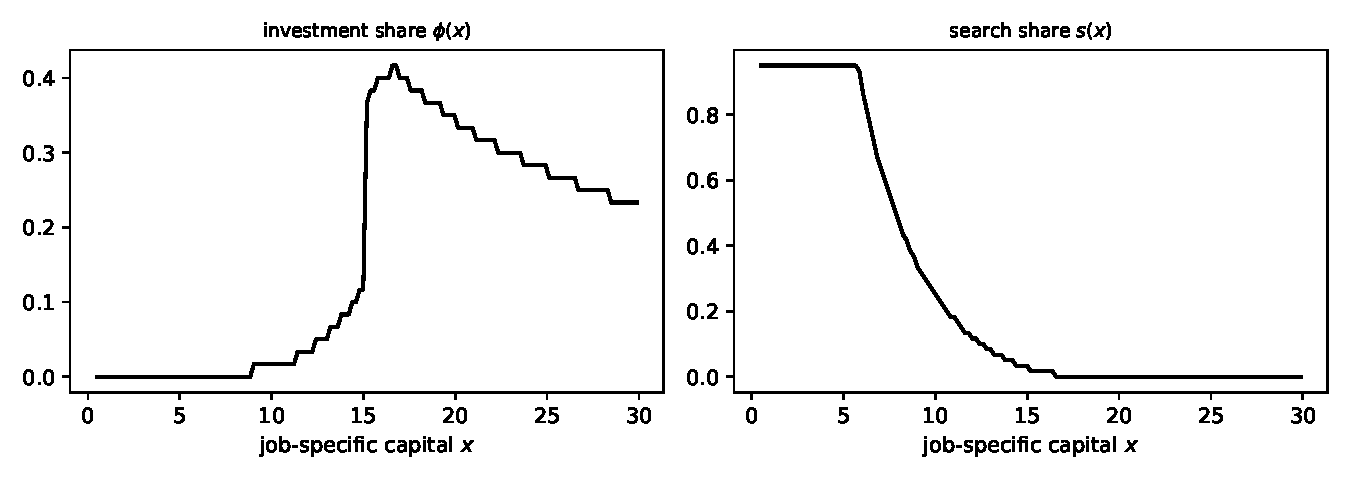
\includegraphics[width=0.88\textwidth]{figures/ch6_18.pdf}\\
{\small Figure S6.1. Optimal investment and search shares as functions of job-specific capital.}
\end{center}
The policies split jobs into bad and good matches.  In a poor match ($x\lesssim6$) the worker searches as hard as possible and does not invest: the capital is
not worth building, and the job is a waiting room.  Search intensity falls steeply as $x$ rises.  Above $x\approx15$ the worker stops searching and invests heavily ($\phi$ jumps
to about $.4$), and capital grows toward a stable level near $x\approx21$ where investment just offsets depreciation.  Below $x\approx15$, capital drifts down while the
worker searches.  Turnover is thus concentrated among young (low-$x$) matches, which is Jovanovic's explanation for the declining separation rate with tenure.
\end{ex}

%%---------------------------------------------------------------------------
\begin{ex}{6.19}{Value function iteration versus policy improvement}
\textbf{(a)}  $v(w)=\max\{w/(1-\beta),\,c+\beta\int v\,dF\}$.  The reservation wage satisfies $w^*-c=\frac\beta{1-\beta}S(w^*)$ (see the notation above).

\textbf{(b)}  Start from any $v_0$ with $\int v_0\,dF$ finite.  Each iterate $v_{n+1}(w)=\max\{w/(1-\beta),c+\beta\int v_ndF\}$ compares an increasing function with a constant,
so its policy is ``accept iff $w\ge w_{n+1}=(1-\beta)(c+\beta\int v_ndF)$.''  From $n\ge1$ on, $v_n(w)=\max\{w,w_n\}/(1-\beta)$, so
\[
  w_{n+1}=T(w_n)\equiv(1-\beta)c+\beta\,E\max\{w,w_n\},\qquad T'(w)=\beta F(w)\le\beta .
\]
$T$ is a contraction with modulus $\beta$ whose fixed point is $w^*$, and
\[
  |w_{n+1}-w^*|\le\beta F(\max\{w_n,w^*\})\,|w_n-w^*| .
\]
Convergence is linear, asymptotically at rate $\beta F(w^*)\le\beta$.

\textbf{(c)}  Given the policy ``accept iff $w\ge w_n$,'' its value before drawing solves
\[
  Q_n=c+\beta\Bigl[F(w_n)Q_n+\int_{w_n}^B\frac{w'}{1-\beta}\,dF(w')\Bigr].
\]
The improvement step compares $w/(1-\beta)$ with the constant $Q_n$, which is again a reservation-wage policy, with
\[
  w_{n+1}=H(w_n)\equiv\frac{(1-\beta)c+\beta\int_{w_n}^Bw'\,dF(w')}{1-\beta F(w_n)} .
\]
$H(w^*)=w^*$ is equivalent to the reservation equation.  Differentiating (with density $f$),
\[
  H'(w)=\frac{\beta f(w)\,[H(w)-w]}{1-\beta F(w)}\quad\Rightarrow\quad H'(w^*)=0,\qquad H''(w^*)=-\frac{\beta f(w^*)}{1-\beta F(w^*)} .
\]
A Taylor expansion gives $w_{n+1}-w^*\cong K(w_n-w^*)^2$ with
\[
  K=\tfrac12H''(w^*)=-\frac{\beta f(w^*)}{2[1-\beta F(w^*)]} .
\]
(Howard's algorithm is Newton's method, hence quadratic.)  \emph{Numerical check} (\texttt{ch6.py}; $F$ uniform on $[0,1]$, $\beta=.95$, $c=.5$, so $w^*=0.817256$ and
$K=-2.1243$), starting both methods from $w_0=0$:
\begin{center}
\begin{tabular}{rccc}
\toprule
$n$ & VFI $w_n-w^*$ & Howard $w_n-w^*$ & $(w_n-w^*)/(w_{n-1}-w^*)^2$ (Howard)\\
\midrule
1 & $-3.2\times10^{-1}$ & $-3.2\times10^{-1}$ & ---\\
2 & $-2.0\times10^{-1}$ & $-9.1\times10^{-2}$ & $-0.905$\\
3 & $-1.4\times10^{-1}$ & $-1.3\times10^{-2}$ & $-1.532$\\
4 & $-9.6\times10^{-2}$ & $-3.3\times10^{-4}$ & $-2.016$\\
5 & $-7.0\times10^{-2}$ & $-2.2\times10^{-7}$ & $-2.121$\\
8 & $-3.0\times10^{-2}$ & $<10^{-13}$ & \\
\bottomrule
\end{tabular}
\end{center}
The value-iteration error shrinks by a factor approaching $\beta w^*=0.776$ per step, and the Howard ratio converges to $K$.
\end{ex}

%%---------------------------------------------------------------------------
\begin{ex}{6.20}{Riskier offer distributions}
\textbf{(a)}  $v(w)=\max\{w/(1-\beta),\,c+\beta\int v\,dF_\alpha\}$.  The problem is stationary (the same distribution and payoffs every period, no recall), so the
value of rejecting is the same constant every period.  The policy is a single reservation wage $\bar w_\alpha$ with
$\bar w_\alpha-c=\frac\beta{1-\beta}\int_{\bar w_\alpha}^B(w-\bar w_\alpha)dF_\alpha$.

\textbf{(b)}  Every $F_\alpha$ has mean $B/2$: $\int_{\alpha B}^{B-\alpha B}\frac wB\,dw+\alpha B=\frac B2$.  Moreover $F_\alpha-F_0$ equals $\alpha-w/B\ge0$ on $[0,\alpha B]$, $0$ on the middle
interval, and $1-\alpha-w/B\le0$ on $[B-\alpha B,B)$.  So $\int_0^y(F_\alpha-F_0)\ge0$ for all $y$, with equality at $y=B$: $F_\alpha$ is a mean-preserving spread of the uniform $F_0$
(conditions (i) and (iii) of section \bk{6.2.2}).  By the argument of section \bk{6.3.2}, using $w-c=\beta(Ew-c)+\beta\int_0^wF$, the spread raises the reservation wage.
Here the inequality is strict, because $\int_0^y(F_{.3}-F_0)>0$ for $0<y<B$ and $\bar w\in(c,B)$.  The $\alpha=.3$ worker has the higher reservation wage.

\textbf{(c)}  Ambiguous in general.  The acceptance probability is $1-F_\alpha(\bar w_\alpha)$, and a higher reservation wage by itself lowers it.  But under $F_{.3}$ the offers
bunch at the top.  With $B=1$ and $\beta=.95$ (\texttt{ch6.py}):
\begin{center}
\begin{tabular}{lcccc}
\toprule
$c$ & $\bar w_0$ & $\Prob(\text{accept})$, $\alpha=0$ & $\bar w_{.3}$ & $\Prob(\text{accept})$, $\alpha=.3$\\
\midrule
$.05$ & $0.732$ & $0.268$ & $0.858$ & $0.300$\\
$.50$ & $0.817$ & $0.183$ & $0.925$ & $0.300$\\
$.80$ & $0.898$ & $0.102$ & $0.970$ & $0.300$\\
\bottomrule
\end{tabular}
\end{center}
The $\alpha=.3$ worker waits for the top offer $w=B$ (her reservation wage exceeds $.7B$), which arrives with probability $.3$.  That is more often than the uniform
worker accepts, so the riskier-distribution worker finds a job \emph{faster}.  With a much lower $\beta$ (a less patient worker) $\bar w_0$ falls toward $c$, and the ranking
can reverse.
\end{ex}

%%---------------------------------------------------------------------------
\begin{ex}{6.21}{Searching for the lowest price}
\textbf{(a)}  Let $V$ be the minimal expected total outlay (price plus remaining search costs) before a draw.  Then $V=c+E\min\{p,V\}$: buy at $p$ if $p\le V$,
otherwise draw again.  Rearranging,
\[
  c=E(V-p)^+=\int_{\underline B}^{V}(V-p)\,dF(p)=\int_{\underline B}^{V}F(p)\,dp .
\]
The right side increases continuously from $0$ at $V=\underline B$ to $\bar B-Ep$ at $V=\bar B$, so there is a unique solution $p^*=V$ if $c<\bar B-Ep$ (otherwise buy at the first
draw).  The strategy is to buy at the first price $p\le p^*$, the reservation price.

\textbf{(b)}  The expected price plus search costs is $V=p^*$.  Equivalently, the number of draws is geometric with mean $1/F(p^*)$, the expected price
paid is $E[p\given p\le p^*]$, and $E[p\given p\le p^*]+c/F(p^*)=p^*$, because $c=F(p^*)\,(p^*-E[p\given p\le p^*])$ by the equation in (a).
\end{ex}

%%---------------------------------------------------------------------------
\begin{ex}{6.22}{Quits}
\textbf{(a)}  Let $J(w)$ be the value of working at $w$ this period, and $Q=\int v\,dF$ the value of an unemployed worker before drawing:
\[
  v(w)=\max\{J(w),\,c+\beta Q\},\qquad J(w)=w+\beta\bigl[(1-\alpha)J(w)+\alpha Q\bigr].
\]
After a reclassification the worker faces exactly the problem of an unemployed worker holding an offer.  So $J(w)=[w+\beta\alpha Q]/[1-\beta(1-\alpha)]$, which
is increasing in $w$.

\textbf{(b)}  Accept iff $J(w)\ge c+\beta Q$, i.e.\ iff $w\ge\bar w$.

\textbf{(c)}  A reclassified worker holding $w'$ makes the same comparison, so he quits iff $w'<\bar w$; a worker who is not reclassified never quits.  Eliminating $Q$,
using $(1-\beta)Q=c+S(\bar w)/[1-\beta(1-\alpha)]$, gives
\[
  \bar w-c=\frac{\beta(1-\alpha)}{1-\beta(1-\alpha)}\int_{\bar w}^B(w-\bar w)\,dF(w),
\]
McCall's equation with the effective discount factor $\beta(1-\alpha)$: jobs are less durable, which lowers the reservation wage.

\textbf{(d)}  Solve the last equation for $\bar w$.  The per-period quit probability of an employed worker is $\alpha F(\bar w)$ (reclassified, then drawing below $\bar w$).
\end{ex}

%%---------------------------------------------------------------------------
\begin{ex}{6.23}{A career ladder}
\textbf{(a)}  $V(w)=(1-\alpha)[w+\beta V(w)]+\alpha[\gamma w+\beta V(\gamma w)]$.  Guessing $V(w)=\kappa w$ gives $\kappa=(1+\beta\kappa)m$ with $m\equiv1-\alpha+\alpha\gamma$ (the expected
gross wage growth), so $\kappa=m/(1-\beta m)$, provided $\beta m<1$.

\textbf{(b)}  Accepting $w$ yields $w+\beta V(w)=w/(1-\beta m)$.  So $v(w)=\max\{w/(1-\beta m),\,c+\beta\int v\,dF\}$.

\textbf{(c)}  Accept iff $w\ge\bar w=(1-\beta m)(c+\beta Q)$.  Equivalently, $(1-\beta)\bar w=(1-\beta m)c+\beta S(\bar w)$, the model of exercise 6.8 with growth factor $m$.  Better promotion
prospects lower the reservation wage when $c>0$.

\textbf{(d)}  An employed worker never wants to leave.  His wage only rises, and a job he accepted was already better than continued search.  If quitting were
allowed, he would never exercise the option.
\end{ex}

%%---------------------------------------------------------------------------
\begin{ex}{6.24}{Human capital}
\textbf{(a)}  Let $A(w,h)$ be the value of working this period at $w$ with human capital $h$, $U(h)$ the value of an unemployed worker about to draw an offer, and
$V^e(w,h)$ the value of a worker employed last period at $w$ after seeing his new $h$:
\begin{align*}
  A(w,h)&=wh+\beta\sum_{h'}H_e(h,h')\,V^e(w,h'),\qquad V^e(w,h)=\max\{A(w,h),\,U(h)\},\\
  U(h)&=\int\max\Bigl\{A(w,h),\;c+\beta\sum_{h'}H_u(h,h')\,U(h')\Bigr\}\,dF(w).
\end{align*}

\textbf{(b)}  $A(w,h)$ is increasing in $w$, so there are $h$-dependent reservation wages.  An unemployed worker accepts iff $w\ge w^u(h)$, where
$A(w^u(h),h)=c+\beta E_uU(h')$.  An employed worker quits iff $w<w^e(h)$, where $A(w^e(h),h)=U(h)$.  Since $U(h)\ge c+\beta E_uU(h')$ (the option to draw now
includes the option to reject), $w^e(h)\ge w^u(h)$.  Employed workers may quit.  While employed, $h$ tends to grow, so the value $U(h)$ of drawing a fresh $w$ (which
multiplies the higher $h$) rises, and a worker with a low $w$ may find it optimal to quit and redraw.  A worker may even accept a low $w\in[w^u(h),w^e(h))$ as a
temporary job, to keep his human capital from decaying, and quit and redraw later.

\textbf{(c)}  Discretize $w$ (on the support of $F$) and use the grid $\bar h_1,\dots,\bar h_n$.  Iterate on the pair $(V^e,U)$: given $(V^e_k,U_k)$, compute $A_k$ from the first
equation, $U_{k+1}$ from the third and $V^e_{k+1}=\max\{A_k,U_{k+1}\}$.  The mapping is a contraction with modulus $\beta$ in the sup norm.  Stop when successive iterates are close,
then read off $w^u(h)$ and $w^e(h)$ as the smallest $w$ on the grid satisfying the acceptance and staying conditions.
\end{ex}

%%---------------------------------------------------------------------------
\begin{ex}{6.25}{Markov wages}
\textbf{(a)}  $v(i)=\max\bigl\{w_i/(1-\beta),\;c+\beta\sum_jP_{ij}v(j)\bigr\}$, $i=1,\dots,5$.

\textbf{(b)}  No, not in general.  The value of rejecting, $c+\beta(Pv)_i$, now depends on the current offer, because today's offer forecasts tomorrow's.  The acceptance set
$\{i:w_i/(1-\beta)\ge c+\beta(Pv)_i\}$ is an upper interval if $w_i/(1-\beta)-\beta(Pv)_i$ is increasing in $i$.  That holds, for instance, when offers are i.i.d.\ (identical
rows of $P$), but nothing guarantees it in general.  With the given $P$ it fails: from $w=3$ the next offer is $1,2,4$ or $5$ with equal probability, so state 3 is a
springboard.

\textbf{(c), (d)}  Value iteration gives:
\begin{center}
\begin{tabular}{lccccc}
\toprule
$w_i$ & 1 & 2 & 3 & 4 & 5\\
\midrule
$\beta=.95$: $v(i)$ & $35.83$ & $40.00$ & $61.83$ & $80.31$ & $100.00$\\
\phantom{$\beta=.95$:} accept? & no & \textbf{yes} & no & no & \textbf{yes}\\
$\beta=.99$: $v(i)$ & $224.19$ & $230.46$ & $352.80$ & $466.76$ & $500.00$\\
\phantom{$\beta=.99$:} accept? & no & no & no & no & \textbf{yes}\\
\bottomrule
\end{tabular}
\end{center}

\textbf{(e)}  With $\beta=.95$ the optimal policy is \emph{not} a reservation wage: the worker accepts $2$ and $5$ but rejects $3$ and $4$.  From $w=2$ the chain mostly stays at
low wages (it moves up to $3$ with probability only $.02$), so the worker grabs the job.  From $3$ the next offer is a lottery over $\{1,2,4,5\}$ whose option value exceeds
$3/(1-\beta)=60$.  From $4$ the chain stays near the top ($4$ or $5$), so waiting for $5$ is worth more than $80$.  With $\beta=.99$ the worker is patient enough to hold out for the
best wage from every state: the acceptance set shrinks to $\{5\}$, which here is a reservation-wage policy.  More patience raises the value of waiting for the
absorbing-like top state relative to locking in a lower wage.
\end{ex}

%%---------------------------------------------------------------------------
\begin{ex}{6.26}{Markov implications of Neal's model}
\textbf{(a)}  \emph{Row 3}: a worker who stays put keeps $(\theta,\epsilon)$ forever, so $P_{33}=1$.  \emph{Row 2}: the new-job region lies in $\theta\ge\bar\theta$, where the worker never
abandons the career (section \bk{6.5}).  Keeping $\theta$, he draws $\epsilon'\sim G$ and next period stays put iff $\epsilon'\ge\bar\epsilon$, where the reservation job $\bar\epsilon$ from \bk{(6.5.5)} is
\emph{independent of} $\theta$.  So $P_{21}=0$, $P_{23}=1-G(\bar\epsilon)$ and $P_{22}=G(\bar\epsilon)$, the same for every $\theta$ in the region.  That is what makes the partition
Markov.  \emph{Row 1}: a new pair is drawn from $F\times G$, so $P_{1j}$ is the $F\times G$ probability of region $j$ of Figure \bk{6.5.2}.

Solving Neal's model on the book's grid (50 equally spaced values on $[0,5]$ for each of $\theta$ and $\epsilon$, $\beta=.95$; \texttt{ch6.py}) reproduces Figure \bk{6.5.2} (our Figure S6.2),
with $\bar\theta=3.98$ and $\bar\epsilon=4.18$, and gives
\[
  P=\begin{bmatrix}0.7620&0.1804&0.0576\\0&0.82&0.18\\0&0&1\end{bmatrix}.
\]
\begin{center}
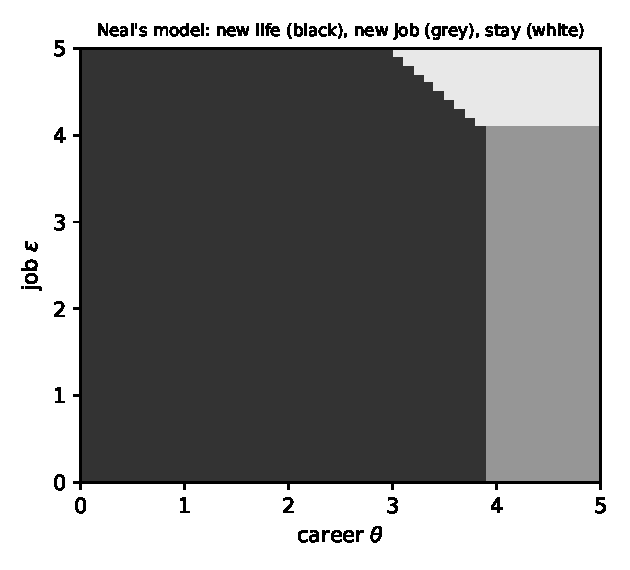
\includegraphics[width=0.42\textwidth]{figures/ch6_26.pdf}\\
{\small Figure S6.2. Decision regions of Neal's model (compare Figure 6.5.2 of the book).}
\end{center}

\textbf{(b)}  States 1 and 2 are transient ($P_{11},P_{22}<1$) and state 3 is absorbing.  The unique invariant distribution is $(0,0,1)'$.

\textbf{(c)}  Yes.  The invariant distribution is unique and concentrated on state 3, so every invariant function is constant on its support.  Along any path the worker
settles down in finite time.  The expected number of periods before settling is finite: $1/(1-P_{11})=4.2$ periods in state 1, plus the time spent in state 2.

\textbf{(d)}  Each observed transition reveals the state: a switch of both job and occupation between $t$ and $t+1$ means $s_t=1$; a job switch within the occupation means
$s_t=2$; no switch means $s_t=3$.  With the counts $n_{ij}$ of consecutive pairs $(s_t,s_{t+1})=(i,j)$, the maximum likelihood estimator of a Markov chain is
$\hat P_{ij}=n_{ij}/\sum_kn_{ik}$.  The model implies zero restrictions ($P_{21}=P_{31}=P_{32}=0$), which can be imposed, or tested with a likelihood ratio test:
Neal's data show some late career switches, which reject them.  Given parametric forms for $F$ and $G$, one can go further and estimate the primitives by
matching $P_{12},P_{13},P_{23}$ (or by maximum likelihood).
\end{ex}

%%---------------------------------------------------------------------------
\begin{ex}{6.27}{Neal's model with unemployment}
\textbf{(a)}
\[
  v(\theta,\epsilon)=\max\Bigl\{\theta+\epsilon+\beta v(\theta,\epsilon),\;c+\beta\int v(\theta,\epsilon')\,dG(\epsilon'),\;c+\beta\int\!\!\int v(\theta',\epsilon')\,dF(\theta')\,dG(\epsilon')\Bigr\}.
\]

\textbf{(b)}  Let $C(\theta)=c+\beta\int v(\theta,\epsilon')dG$ and $Q=c+\beta\int\!\!\int v\,dF\,dG$.  As in Neal's model, $v$ is increasing, $C(\theta)$ is increasing in $\theta$, and the worker keeps his
career iff $C(\theta)\ge Q$, i.e.\ iff $\theta\ge\bar\theta$.  He stays put iff $(\theta+\epsilon)/(1-\beta)\ge\max\{C(\theta),Q\}$.  The important difference is \emph{within} a kept career.  There the worker
solves $W(\theta,\epsilon)=\max\{(\theta+\epsilon)/(1-\beta),\,c+\beta\int W(\theta,\epsilon')dG\}$.  While searching for a job he forgoes his career income $\theta$, so this is McCall's problem
for the offer $\epsilon$ with effective compensation $c-\theta$:
\[
  \bar\epsilon(\theta)-(c-\theta)=\frac\beta{1-\beta}\int_{\bar\epsilon(\theta)}(\epsilon'-\bar\epsilon(\theta))\,dG(\epsilon'),\qquad
  \frac{d\bar\epsilon}{d\theta}=-\frac1{1+\beta[1-G(\bar\epsilon)]/(1-\beta)}\in(-1,0).
\]
So the reservation job quality \emph{falls} with the quality of the career.  (In Neal's original model $\bar\epsilon$ is independent of $\theta$, because a job switch costs nothing
there.)  Higher $c$ lowers the cost of switching: it raises $\bar\epsilon(\theta)$ and $\bar\theta$ and enlarges the switching regions.  With the grids of exercise 6.26
(\texttt{ch6.py}), $c=0$ gives $\bar\theta=3.57$, and $\bar\epsilon$ falls from $3.16$ to $3.06$ as $\theta$ rises from $3.57$ to $5$.  With $c=2$, $\bar\theta=3.78$ and $\bar\epsilon$ falls from
$3.47$ to $3.37$, in line with the formula (up to grid discreteness).  Because $\bar\epsilon$ now depends on $\theta$, the three-state chain of exercise 6.26 is no longer
exactly Markov: the probability of settling after a job switch depends on the career.
\end{ex}

%% ===========================================================================
%% Chapter 7. Recursive Competitive Equilibrium: I
%% ===========================================================================
\solchapter{7}{Recursive Competitive Equilibrium: I}

\begin{center}
\begin{minipage}{0.86\textwidth}
\small
Solutions to all 7 exercises of Chapter 7 of Ljungqvist and Sargent, \emph{Recursive Macroeconomic Theory} (4th edition, 2018).
The Matlab programs \texttt{olrp.m} and \texttt{nash.m} are replaced by the Python function \texttt{olrp} (\texttt{code/rmtlib.py}) and a best-response
iteration in \texttt{code/ch7.py}, which prints every number below.
\end{minipage}
\end{center}

\bigskip
\hrule
\bigskip

Throughout exercises 7.1--7.5: $A_0=100$, $A_1=.05$, $\beta=.95$, $d=10$.  We solve linear regulators in the minimization form
$\min\sum\beta^t(x_t'Rx_t+u_t'Qu_t)$, $x_{t+1}=Ax_t+Bu_t$, so that a maximized value is $-x'Px$.

%%---------------------------------------------------------------------------
\begin{ex}{7.1}{A competitive firm}
\textbf{(a)}  $v(y,Y)=\max_{y'}\bigl\{A_0y-A_1yY-.5d(y'-y)^2+\beta v(y',Y')\bigr\}$ subject to $Y'=H_0+H_1Y$.

\textbf{(b)}  State $x=(y,\,Y,\,1)'$ (own output, market output and a constant), control $u=y'-y$:
\[
  A=\begin{bmatrix}1&0&0\\0&H_1&H_0\\0&0&1\end{bmatrix},\quad B=\begin{bmatrix}1\\0\\0\end{bmatrix},\quad
  R=\begin{bmatrix}0&A_1/2&-A_0/2\\A_1/2&0&0\\-A_0/2&0&0\end{bmatrix},\quad Q=\frac d2 ,
\]
so that $-(x'Rx+u'Qu)=A_0y-A_1yY-.5du^2$.

\textbf{(c)}  \texttt{olrp} converges in 489 iterations to
\[
  y_{t+1}=96.9487+1.0000\,y_t-0.046282\,Y_t .
\]
The coefficient on the firm's own output is exactly one.  The firm's return is linear in its own $y$, so, as in exercise 5.11, the \emph{change} in output depends only on
the forecast of future prices, i.e.\ on $Y_t$, and not on $y_t$.

\textbf{(d)}  With $Y_t=ny_t$, $Y_{t+1}=n(h_0+h_1Y_t/n+h_2Y_t)=nh_0+(h_1+nh_2)Y_t$.  For $n=1$: $Y_{t+1}=96.9487+0.953718\,Y_t$, which differs from the perceived
$(95.5,.95)$, so these beliefs are not rational.

\textbf{(e)}  The first-order condition for $y_{t+1}$, combined with the envelope condition $v_y(y,Y)=A_0-A_1Y+d(y'-y)$, gives
\[
  -d(y_{t+1}-y_t)+\beta\bigl[A_0-A_1Y_{t+1}+d(y_{t+2}-y_{t+1})\bigr]=0,
\]
to be solved with $y_0$ given and the transversality condition $\lim_t\beta^ty_tv_y(y_t,Y_t)=0$.
\end{ex}

%%---------------------------------------------------------------------------
\begin{ex}{7.2}{Rational expectations}
With $y=Y$, the perceived law is reproduced iff $h_0=H_0$ and $h_1+h_2=H_1$ (the map $M$ of section \bk{7.2}).

\textbf{(a)}
\begin{center}
\begin{tabular}{lcc}
\toprule
perceived $(H_0,H_1)$ & implied actual $(h_0,\,h_1+h_2)$ & equilibrium?\\
\midrule
(i) $(94.0888,\ .9211)$ & $(118.4668,\ .964986)$ & no\\
(ii) $(93.22,\ .9433)$ & $(104.7364,\ .956861)$ & no\\
(iii) $(95.08187459,\ .95245906)$ & $(95.08187459,\ .95245906)$ & \textbf{yes}\\
\bottomrule
\end{tabular}
\end{center}
Only (iii) is a fixed point (to $10^{-12}$).  Its steady state is $H_0/(1-H_1)=2000=A_0/A_1$, where price is zero, as the Euler equation requires in a steady state.

\textbf{(b)}  Start from a guess $H^{(0)}$.  Given $H^{(k)}$, solve the firm's regulator (exercise 7.1) to get $(h_0,h_1,h_2)$, compute $M(H^{(k)})=(h_0,h_1+h_2)$, and update
$H^{(k+1)}=(1-\gamma)H^{(k)}+\gamma M(H^{(k)})$ with a relaxation parameter $\gamma\in(0,1]$, until $|H^{(k+1)}-H^{(k)}|$ is negligible.  $M$ is not a contraction, so damping ($\gamma<1$)
may be needed.  With $\gamma=.5$, starting from $(95.5,.95)$, the iteration converges to (iii) in 22 steps.
\end{ex}

%%---------------------------------------------------------------------------
\begin{ex}{7.3}{Maximizing welfare}
\textbf{(a)}  $V(Y)=\max_{Y'}\{A_0Y-\frac{A_1}2Y^2-.5d(Y'-Y)^2+\beta V(Y')\}$.

\textbf{(b)}  State $x=(Y,1)'$, control $u=Y'-Y$, $A=I_2$, $B=(1,0)'$, $R=\begin{bmatrix}A_1/2&-A_0/2\\-A_0/2&0\end{bmatrix}$, $Q=d/2$.  The solution is
\[
  Y_{t+1}=95.0818745922+0.952459062704\,Y_t ,
\]
with $V(Y)=-0.262705Y^2+1050.82Y+949181$.

\textbf{(c)}  $(s_0,s_1)$ equals the rational expectations equilibrium (iii) of exercise 7.2 to every digit.  The planner's Euler equation,
$-d(Y_{t+1}-Y_t)+\beta[A_0-A_1Y_{t+1}+d(Y_{t+2}-Y_{t+1})]=0$, is the firm's Euler equation with $y=Y$ imposed.  So the competitive equilibrium maximizes the sum of
consumer and producer surplus, and solving the planning problem is a reliable way to compute the equilibrium (section \bk{7.2.1}).
\end{ex}

%%---------------------------------------------------------------------------
\begin{ex}{7.4}{Monopoly}
\textbf{(a)}  $V(Y)=\max_{Y'}\{A_0Y-A_1Y^2-.5d(Y'-Y)^2+\beta V(Y')\}$.

\textbf{(b)}  The regulator of exercise 7.3 with $R=\begin{bmatrix}A_1&-A_0/2\\-A_0/2&0\end{bmatrix}$ gives
\[
  Y_{t+1}=73.4729+0.926527\,Y_t,\qquad\text{steady state }\frac{73.4729}{1-0.926527}=1000 .
\]

\textbf{(c)}  The monopolist's problem is the planner's with the slope of demand doubled: it maximizes revenue, whose derivative is marginal revenue
$A_0-2A_1Y$, instead of total surplus, whose derivative is price.  Output converges to $A_0/(2A_1)=1000$, half the efficient steady state $2000$.  Output also
adjusts faster, with root $.9265$ versus $.9525$, because the monopolist's objective is more concave in $Y$.
\end{ex}

%%---------------------------------------------------------------------------
\begin{ex}{7.5}{Duopoly}
\textbf{(a)}  With state $x=(y_1,y_2,1)'$, a (linear) Markov perfect equilibrium is a pair of rules $y_{i,t+1}=f_i(x_t)$ and value functions $v_i$ such that, for each $i$, $v_i$ solves
firm $i$'s Bellman equation given that the rival uses $f_j$, and $f_i$ attains the maximum.  Each firm's rule is a best response to the other's, and strategies
depend only on the current state.

\textbf{(b)}  $v_1(y_1,y_2)=\max_{y_1'}\{(A_0-A_1(y_1+y_2))y_1-.5d(y_1'-y_1)^2+\beta v_1(y_1',f_2(y_1,y_2))\}$, and symmetrically for firm 2.

\textbf{(c)}  In regulator form $x_{t+1}=x_t+B_1u_{1t}+B_2u_{2t}$ with $u_i=y_i'-y_i$, $B_1=e_1$, $B_2=e_2$.  Firm 1 has
$R_1=\begin{bmatrix}A_1&A_1/2&-A_0/2\\A_1/2&0&0\\-A_0/2&0&0\end{bmatrix}$ and $Q_1=d/2$ (firm 2 symmetric).  Given $u_2=-F_2x$, firm 1 solves a regulator with
transition matrix $A-B_2F_2$ (equations \bk{(7.7.4)}--\bk{(7.7.7)} in their infinite-horizon form).  Iterating best responses to convergence (12 rounds,
$|F_1-\mathrm{BR}(F_2)|<10^{-12}$) gives the symmetric equilibrium
\[
  y_{i,t+1}=65.2742+0.932925\,y_{it}-0.024230\,y_{jt},\qquad i\ne j .
\]
Each firm reduces its output when its rival's output is high.  Steady-state output is $714.90$ per firm, $1429.80$ for the industry, with closed-loop roots $0.957$ and $0.909$.
\begin{center}
\begin{tabular}{lcccc}
\toprule
 & monopoly & static Cournot & duopoly (MPE) & competition\\
\midrule
steady-state output & $1000$ & $1333.3$ & $1429.8$ & $2000$\\
\bottomrule
\end{tabular}
\end{center}
The dynamic duopoly produces \emph{more} than the static Cournot outcome.  Adjustment costs make current output a commitment to future output, and a rival
cuts its own output when it sees a higher $y_j$.  So each firm expands output strategically to discourage the other (a Markov perfect ``capacity''
effect).
\end{ex}

%%---------------------------------------------------------------------------
\begin{ex}{7.6}{Self-control}
\textbf{(a)}  A Markov perfect equilibrium is a sequence of consumption rules $\{c_t(k)\}_{t=0}^T$, each depending only on the current capital stock, such that for every
$t$ and every $k$, $c_t(k)$ maximizes personality $t$'s utility $u(c)+\delta\sum_{j\ge1}\beta^ju(c_{t+j})$ subject to $k_{t+1}=f(k)-c$, when the later personalities use the rules
$c_{t+1}(\cdot),\dots,c_T(\cdot)$.  Since the definition applies at every $k$, it requires optimality off the equilibrium path too (subgame perfection).

\textbf{(b)}  Index personalities by the number $j$ of periods remaining after them, so personality $T-j$ is the $j$th from the end.  Let $W_j(k)$ be the
\emph{exponentially discounted} value $u(c_{T-j})+\beta u(c_{T-j+1})+\dots+\beta^ju(c_T)$ generated by the equilibrium rules from capital $k$ at date $T-j$.  The last personality
consumes everything: $c_0(k)=f(k)$ and $W_0(k)=u(f(k))$.  Personality $T-j-1$ weighs date $T-j-1+s$ by $\delta\beta^s$ for $s\ge1$.  Given the later rules, its objective is
therefore $u(c)+\delta\beta W_j(f(k)-c)$, so its value and rule are
\[
  V_{j+1}(k)=\max_c\bigl\{u(c)+\beta\delta W_j(f(k)-c)\bigr\},\qquad c_{j+1}(k)=\arg\max .
\]
To continue the induction, earlier personalities need the exponentially discounted continuation, which follows the rule $c_{j+1}$:
$W_{j+1}(k)=u(c_{j+1}(k))+\beta W_j(f(k)-c_{j+1}(k))$.  The factor $\delta$ appears once, between ``now'' and ``later''.  All dates after the next are weighted relative to each other by
$\beta$ alone, which is why $W$, not $V$, is the right object to carry backward.  With $\delta=1$, $V_j=W_j$ and this is ordinary dynamic programming.

\textbf{(c)}  The time-0 dictator chooses $\{c_t\}_{t=0}^T$ to maximize $u(c_0)+\delta\sum_{t=1}^T\beta^tu(c_t)$ subject to $k_{t+1}=f(k_t)-c_t$.  From date 1 on the weights $\delta\beta^t$ are
proportional to $\beta^{t-1}$, so the continuation is a standard problem.  Let $J_0(k)=u(f(k))$ and
\[
  J_{s+1}(k)=\max_c\{u(c)+\beta J_s(f(k)-c)\},\qquad s=0,\dots,T-1,
\]
and at date 0 solve $\max_{c_0}\{u(c_0)+\delta\beta J_T(f(k_0)-c_0)\}$.  The plan uses the time-consistent exponential rules from date 1 on.  With commitment, later
personalities cannot re-optimize, and they would want to if $\delta<1$.  This is the value of a ``self-control'' technology.
\end{ex}

%%---------------------------------------------------------------------------
\begin{ex}{7.7}{Equilibrium search}
\textbf{(a)}  Let $U'=G(U)$ be the law of motion that workers perceive.  Let $v(w,U)$ be the value of an unemployed worker holding offer $w$, $Q(U)=\int v(w',U)\,dF(w')$ the value of
drawing an offer, and $E(w,U)$ the value of a worker employed at $w$ at the start of a period, before the firing draw:
\[
  v(w,U)=\max\bigl\{w+\beta E(w,G(U)),\;c(U)+\beta Q(G(U))\bigr\},
\]
\[
  E(w,U)=(1-\lambda)\bigl[w+\beta E(w,G(U))\bigr]+\lambda Q(U).
\]

\textbf{(b)}  $E(w,U)$ is increasing in $w$, while the value of rejecting does not depend on $w$.  So the rule is a reservation wage that depends on the aggregate state:
accept iff $w\ge\bar w(U)$, where $\bar w(U)+\beta E(\bar w(U),G(U))=c(U)+\beta Q(G(U))$.  Since $c(U)$ rises with $U$, unemployment is more attractive when unemployment is
high.  Future labor-market conditions enter through $G(U)$.

\textbf{(c)}  With a continuum of workers and i.i.d.\ draws, the law of large numbers gives $\phi(U)=1-F(\bar w(U))$, the probability that a draw exceeds the reservation
wage.

\textbf{(d)}  A recursive competitive equilibrium is a set of functions $v(w,U)$, $E(w,U)$, $Q(U)$, a reservation wage $\bar w(U)$ and a law of motion $U'=G(U)$ such that:
(i) given $G$, $v$, $E$, $Q$ solve the Bellman equations in (a) and $\bar w(U)$ is the optimal rule; (ii) the perceived law of motion equals the actual one implied by the
workers' decisions:
\[
  G(U)=\lambda(1-U)+F(\bar w(U))\,U .
\]
As in section \bk{7.2}, individual workers take the aggregate law as given, and in equilibrium their collective behavior reproduces it.  A stationary equilibrium
unemployment rate is a fixed point $U^*=G(U^*)$.
\end{ex}

%% ===========================================================================
%% Chapter 8. Equilibrium with Complete Markets
%% ===========================================================================
\solchapter{8}{Equilibrium with Complete Markets}

\begin{center}
\begin{minipage}{0.86\textwidth}
\small
Solutions to all 28 exercises of Chapter 8 of Ljungqvist and Sargent, \emph{Recursive Macroeconomic Theory} (4th edition, 2018).
Numerical results come from \texttt{code/ch8.py}, which also cross-checks them (brute-force sums over histories, bisection on budget
constraints, residuals of Euler equations and budget constraints).
\end{minipage}
\end{center}

\bigskip
\hrule
\bigskip

Notation.  $q^0_t(s^t)$ is the time-0 (Arrow--Debreu) price of a unit of consumption at history $s^t$, normalized by $q^0_0(s_0)=1$; $Q(s'\given s)$ is the
price, in units of today's good, of a one-period Arrow security paying one unit tomorrow if $s_{t+1}=s'$.  With a Markov state and
consumption a function of the state, \bk{(8.9.4)} gives
\[
  Q(s'\given s)=\beta\,\frac{u'(c(s'))}{u'(c(s))}\,P(s,s').
\]
For two states we collect these prices in a matrix $Q$; then \bk{(8.10.3)} says that the $h$-step prices are the entries of $Q^h$.  For
a claim on a Markov dividend $y(s)$ that includes today's dividend, the value $V$ solves $V=y+QV$, so $V=(I-Q)^{-1}y$.  This is also the
formula for the natural debt limits \bk{(8.9.13)}.  In growth economies, $y_{t+1}=\lambda_{t+1}y_t$ with CRRA utility $u(c)=c^{1-\gamma}/(1-\gamma)$, the
one-period prices are $Q_{ij}=\beta P_{ij}\lambda_j^{-\gamma}$, and ratios of values to the current endowment depend only on the state.

%%---------------------------------------------------------------------------
\begin{ex}{8.1}{Family economics, I}
\rmk{The book says that ``person 2 has no labor but is endowed with $s$ units.''  Since $n_2$ is person~2's labor, and exercise 8.2 starts
``instead of being endowed with $s$ units of consumption, household 1 is endowed with 1 unit,'' the sentence should read ``person~1 has no
labor but is endowed with $s$ units.''  This matters only for the ``natural'' distribution of property in (d)--(f).}

\textbf{(a)}  With multiplier $\mu\ge0$ on the resource constraint, and respecting $n_2\ge0$,
\[
  \mathcal L=\lambda_1\log c_1+\lambda_2(\log c_2-n_2)+\mu\,(n_2+s-c_1-c_2).
\]

\textbf{(b)}  The objective is concave and the constraint linear, so the Kuhn--Tucker conditions are sufficient:
\[
  \frac{\lambda_1}{c_1}=\mu,\qquad \frac{\lambda_2}{c_2}=\mu,\qquad \mu-\lambda_2\le0\quad(=0\text{ if }n_2>0).
\]
\emph{Interior case}, $s<1+\lambda_1/\lambda_2$: $\mu=\lambda_2$, so
\[
  c_1=\frac{\lambda_1}{\lambda_2},\qquad c_2=1,\qquad n_2=1+\frac{\lambda_1}{\lambda_2}-s>0 .
\]
\emph{Corner}, $s\ge1+\lambda_1/\lambda_2$: $n_2=0$, the endowment is split in proportion to the weights,
$c_i=\lambda_is/(\lambda_1+\lambda_2)$, and $\mu=(\lambda_1+\lambda_2)/s\le\lambda_2$, as the third condition requires.

\textbf{(c)}  $\mu$ is the increase in family welfare from one more unit of the good: the shadow price of the consumption good (of the
endowment $s$).  When person~2 works, a unit of the good can also be obtained with one unit of her labor, which costs $\lambda_2$ in welfare.
So $\mu=\lambda_2$ is also the shadow wage of her labor.  At the corner the good is abundant and $\mu<\lambda_2$: labor is not worth using.

\textbf{(d)}  Let the good be the numeraire, $p=1$.  A competitive firm with the linear technology $y=n$ earns zero profits only if the wage
is $w=1$.  Give person~1 a claim to $e_1$ units of the good and person~2 the rest of the endowment, $s-e_1$, plus her time.  Each person
then maximizes his or her own utility, $\log c_1$ and $\log c_2-n_2$, subject to $c_1\le e_1$ and $c_2\le s-e_1+wn_2$.  By the second
welfare theorem, the Pareto allocation of (b) is a competitive allocation when $e_1=c_1$: $e_1=\lambda_1/\lambda_2$ in the interior case
and $e_1=\lambda_1s/(\lambda_1+\lambda_2)$ at the corner.  (If $\lambda_1/\lambda_2>s$, person~2's nonlabor wealth $s-e_1$ is negative: she
owes person~1 a lump-sum transfer.)  With the natural property distribution of the remark, person~1 owns all of $s$, $e_1=s$.

\textbf{(e)}  Person~1 consumes his wealth, $c_1=e_1$.  Person~2's first-order conditions $1/c_2=\nu$ and $\nu w=1$ (if $n_2>0$) give
$c_2=w=1$ and $n_2=1-(s-e_1)$.  So the equilibrium is $p=w=1$, $c_1=e_1$, $c_2=1$, $n_2=1+e_1-s$ if $s-e_1<1$; otherwise $n_2=0$ and
$c_2=s-e_1$.  With $e_1=s$: $c_1=s$, $c_2=1$, $n_2=1$.  This is the Pareto optimum with weights $\lambda_1/\lambda_2=s$.

\textbf{(f)}  For fixed Pareto weights, $n_2=\max\{0,\,1+\lambda_1/\lambda_2-s\}$: labor falls one for one with $s$, while consumption does not
change.  Utility is linear in labor, so the whole income effect of a larger endowment falls on labor.  In the competitive economy in which
person~1 owns $s$, instead, $n_2=1$ for every $s$.  The extra endowment then goes to person~1 and does not affect person~2's budget.
The planner, by contrast, pools the endowment and relieves person~2 of work.
\end{ex}

%%---------------------------------------------------------------------------
\begin{ex}{8.2}{Family economics, II}
\rmk{The book says that preferences are those of ``exercise 8.25''; it means exercise 8.1.}

\textbf{(a)}  $\mathcal L=\lambda_1\log c_1+\lambda_2(\log c_2-n_2)+\mu\,(sn_2+1-c_1-c_2)$, with $n_2\ge0$.

\textbf{(b)}  The conditions are $\lambda_1/c_1=\mu=\lambda_2/c_2$ and $s\mu-\lambda_2\le0$, with equality if $n_2>0$.  \emph{Interior case},
$s(1+\lambda_1/\lambda_2)>1$:
\[
  \mu=\frac{\lambda_2}{s},\qquad c_1=\frac{\lambda_1}{\lambda_2}\,s,\qquad c_2=s,\qquad n_2=1+\frac{\lambda_1}{\lambda_2}-\frac1s .
\]
\emph{Corner}, $s(1+\lambda_1/\lambda_2)\le1$: $n_2=0$, $c_i=\lambda_i/(\lambda_1+\lambda_2)$ and $\mu=\lambda_1+\lambda_2\le\lambda_2/s$.

\textbf{(c)}  $\mu$ is the shadow price of the good.  With positive work, $s\mu=\lambda_2$: a unit of labor yields $s$ goods and costs
$\lambda_2$ in welfare, so $\lambda_2$ is the shadow wage and $\mu=\lambda_2/s$ is the labor cost of one more unit of the good.

\textbf{(d)}  Price of the good $p=1$, wage $w=s$ (zero profits for a firm with technology $y=sn$).  Person~1 owns $e_1$ units and
person~2 owns $1-e_1$ plus her time; the natural distribution is $e_1=1$.

\textbf{(e)}  Person~2 solves $\max\log c_2-n_2$ subject to $c_2=1-e_1+sn_2$.  If she works, $s/c_2=1$, so $c_2=s$ and $n_2=1-(1-e_1)/s$.
Person~1 consumes $c_1=e_1$.  With the natural distribution $e_1=1$: $c_1=1$, $c_2=s$, $n_2=1$.  This is the Pareto optimum for
$\lambda_1/\lambda_2=1/s$.  Any interior Pareto optimum is supported by $e_1=\lambda_1s/\lambda_2$.

\textbf{(f)}  For fixed weights, $n_2=\max\{0,\,1+\lambda_1/\lambda_2-1/s\}$ increases with productivity $s$ ($dn_2/ds=1/s^2$): a higher
return to work raises labor, and both members consume more.  In the competitive economy in which person~1 owns the unit endowment, $n_2=1$
whatever $s$ is.  With log utility and no nonlabor income, the income and substitution effects of the wage $s$ cancel.  If person~2 owned
part $e_2=1-e_1>0$ of the endowment, $n_2=1-e_2/s$ would increase with $s$.  Labor responds in the opposite direction to exercise 8.1, where
$s$ was a pure wealth effect.
\end{ex}

%%---------------------------------------------------------------------------
\begin{ex}{8.3}{Existence of a representative consumer}
\emph{Existence and uniqueness.}  The objective $\theta u(c_1)+(1-\theta)w(c-c_1)$ is continuous and strictly concave in $c_1$ on $[0,c]$,
so it has a unique maximizer.  We assume Inada conditions (or that the solution is interior); then $c_1(c,\theta)\in(0,c)$ solves
\[
  \theta u'(c_1)=(1-\theta)w'(c-c_1).
\]
\emph{Concavity.}  Take $c,c'>0$ with optimal allocations $(c_1,c_2)$ and $(c_1',c_2')$, and $\tau\in[0,1]$.  The allocation
$\tau(c_1,c_2)+(1-\tau)(c_1',c_2')$ is feasible for $\tau c+(1-\tau)c'$, so
\[
  v_\theta(\tau c+(1-\tau)c')\ge\theta u(\tau c_1+(1-\tau)c_1')+(1-\theta)w(\tau c_2+(1-\tau)c_2')\ge\tau v_\theta(c)+(1-\tau)v_\theta(c'),
\]
by concavity of $u$ and $w$ (strictly if $c\ne c'$).  $v_\theta$ is also increasing, since more resources can be given to either consumer.

\emph{Derivative.}  By the implicit function theorem applied to the first-order condition, $c_1(c,\theta)$ is differentiable, with
\[
  \frac{\partial c_1}{\partial c}=\frac{(1-\theta)w''(c_2)}{\theta u''(c_1)+(1-\theta)w''(c_2)}\in(0,1).
\]
Differentiating $v_\theta(c)=\theta u(c_1(c,\theta))+(1-\theta)w(c-c_1(c,\theta))$,
\[
  v_\theta'(c)=\theta u'(c_1)\frac{\partial c_1}{\partial c}+(1-\theta)w'(c_2)\Bigl(1-\frac{\partial c_1}{\partial c}\Bigr)=\theta u'(c_1)=(1-\theta)w'(c_2),
\]
using the first-order condition (an envelope theorem).  Moreover
$v_\theta''(c)=\theta u''(c_1)\,\partial c_1/\partial c=\dfrac{\theta(1-\theta)u''w''}{\theta u''+(1-\theta)w''}<0$.

\emph{Interpretation.}  In a complete-markets equilibrium the allocation solves the Pareto problem with $\theta=\mu_1^{-1}/(\mu_1^{-1}+\mu_2^{-1})$.
Then \bk{(8.5.4)} gives $q^0_t(s^t)\propto\beta^t\pi_t(s^t)v_\theta'(Y_t(s^t))$, where $Y_t$ is aggregate consumption: prices are those of a
single consumer with utility $v_\theta$ who consumes the aggregate endowment.  Since $\theta u'(c_1)=(1-\theta)w'(c_2)=v_\theta'(c)$, each
consumer's marginal utility is proportional to the representative consumer's.  The representative consumer's preferences depend on the
distribution of wealth through $\theta$, unless preferences are identical and homothetic.
\end{ex}

%%---------------------------------------------------------------------------
\begin{ex}{8.4}{Term structure of interest rates}
\textbf{(a)}  Let $s^t=(\lambda_0,\dots,\lambda_t)$; then $y_t(s^t)=y_0\lambda_1\cdots\lambda_t$.  A competitive equilibrium (with time-0 trading) is a
price system $\{q^0_t(s^t)\}$ and an allocation $\{c_t(s^t)\}$ such that (i) given the prices, $\{c_t\}$ maximizes
$\sum_t\sum_{s^t}\beta^tu(c_t(s^t))\pi_t(s^t)$ subject to $\sum_t\sum_{s^t}q^0_t(s^t)[c_t(s^t)-y_t(s^t)]\le0$, and (ii) $c_t(s^t)=y_t(s^t)$ for all $t,s^t$.

\textbf{(b)}  Market clearing gives the allocation, $c_t=y_t$.  The first-order condition \bk{(8.5.4)}, normalized by $q^0_0=1$, then gives the
prices
\[
  q^0_t(s^t)=\beta^t\pi_t(s^t\given s_0)\Bigl(\frac{y_t(s^t)}{y_0}\Bigr)^{-\gamma}
  =\prod_{k=1}^t\beta P(\lambda_{k-1},\lambda_k)\lambda_k^{-\gamma}.
\]
So the one-period kernel is $Q_{ij}=\beta P_{ij}\bar\lambda_j^{-\gamma}$, which depends on the state only, and the time-0 price of a date-$j$ claim
contingent on $\lambda_j=\bar\lambda_k$ is $(Q^j)_{i_0k}$.  With these prices the budget holds with equality at $c=y$, and the first-order
conditions are sufficient because $u$ is concave.

\textbf{(c)}  The stationary distribution of $P$ is $\bar\pi=(1-p_{22},1-p_{11})/(2-p_{11}-p_{22})=(3/7,4/7)$, so the unconditional mean gross
growth rate is
\[
  E\lambda=\tfrac37(.98)+\tfrac47(1.03)=1.008571,
\]
i.e.\ $0.857\%$ per period.  (If ``before observing $\lambda_0$'' refers to the given $\pi_\lambda=(.5,.5)$, which is not stationary, the mean
growth rate at $t$ is $\pi_\lambda P^t\bar\lambda'$: $1.005$, $1.00625$, $1.00706,\dots$, converging to $1.008571$.)

\textbf{(d)--(f)}  With $\lambda_0=\bar\lambda_1$ the prices are the entries of row~1 of $Q^j$ and their sums.  Here
$Q=\begin{bmatrix}0.799667&0.180978\\0.149938&0.769158\end{bmatrix}$ and \texttt{ch8.py} gives (checked by brute-force summation over histories):
\begin{center}
\begin{tabular}{lccc}
\toprule
 & $j=0$ & $j=1$ & $j=2$\\
\midrule
(d) riskless & $1$ & $0.980645$ & $0.950526$\\
(e) only if $\lambda_j=.98$ & $1$ & $0.799667$ & $0.666602$\\
(f) only if $\lambda_j=1.03$ & $0$ & $0.180978$ & $0.283923$\\
\bottomrule
\end{tabular}
\end{center}
At $j=0$ the state is known: $\lambda_0=.98$, so the claim in (e) is riskless and the one in (f) pays nothing.

\textbf{(g)}  Each price in (d) is the sum of the prices in (e) and (f).  A riskless claim is a portfolio of the two contingent claims, and
any other price would create an arbitrage.  The riskless yields are $-\log(0.980645)=1.95\%$ for one period and $-\tfrac12\log(0.950526)=2.54\%$
per period for two: the term structure slopes up in the low-growth state, because growth is expected to rise.  Per unit of probability,
claims on the low-growth state are dearer ($0.7997/.8=1.000$ versus $0.1810/.2=0.905$ at $j=1$): they pay when marginal utility is high.
\end{ex}

%%---------------------------------------------------------------------------
\begin{ex}{8.5}{Periodic endowments}
\textbf{(a)}  A price system $\{q_t\}$ and an allocation $\{c^1_t,c^2_t\}$ such that each $\{c^i_t\}$ maximizes $\sum_t\beta^tu(c^i_t)$ subject to
$\sum_tq_tc^i_t\le\sum_tq_ty^i_t$, and $c^1_t+c^2_t=y^1_t+y^2_t$ for all $t$.

\textbf{(b)}  The aggregate endowment is $1$ every period.  The first-order conditions $\beta^tu'(c^i_t)=\mu_iq_t$ give
$u'(c^1_t)/u'(c^2_t)=\mu_1/\mu_2$.  The map $c\mapsto u'(c)/u'(1-c)$ is strictly decreasing, so $c^1_t=\bar c^1$ is constant, and so is
$c^2_t=1-\bar c^1$ (as in section \bk{8.6.3}).  Then $q_t=\beta^tu'(\bar c^1)/\mu_1$, and the normalization $q_0=1$ gives $q_t=\beta^t$.
Consumer~1's budget, $\bar c^1\sum_t\beta^t=\sum_{j\ge0}\beta^{3j}$, gives
\[
  \bar c^1=\frac{1-\beta}{1-\beta^3}=\frac1{1+\beta+\beta^2},\qquad \bar c^2=\frac{\beta+\beta^2}{1+\beta+\beta^2}.
\]
Consumer~2 has two thirds of the endowment but receives it later, so his share is below $2/3$ ($\bar c^2<2/3$ because $\beta<1$).

\textbf{(c)}  By \bk{(8.7.1)} the asset is worth the value of its payouts at the equilibrium prices:
\[
  p=\sum_{t\ge0}.05\,q_t=\frac{.05}{1-\beta}
\]
units of the time-0 good (or $.05\beta/(1-\beta)$ if the first payment is at $t=1$).  The asset is redundant, so issuing it changes neither
the prices nor the allocation.
\end{ex}

%%---------------------------------------------------------------------------
\begin{ex}{8.6}{A Mehra--Prescott economy}
\textbf{(a)}  As in exercise 8.4(a): prices $\{q^0_t(s^t)\}$ and an allocation $\{c_t(s^t)\}$ such that the allocation maximizes expected utility
subject to the single time-0 budget constraint, and $c_t(s^t)=d_t(s^t)$.  In equilibrium
$q^0_t(s^t)=\beta^t\pi_t(s^t)(d_t/d_0)^{-\gamma}$.

\textbf{(b), (c)}  $q^0_5=\beta^5\,\Prob(\lambda_1,\dots,\lambda_5\given\lambda_0)\,d_5^{-\gamma}$:
\begin{align*}
  \text{(b)}\quad &\Prob=P_{11}P_{11}P_{12}P_{21}P_{12}=.00256,\quad d_5=.97^3\,1.03^2=0.968255,\\
  &q^0_5=.95^5(.00256)(0.968255)^{-2}=0.0021129;\\
  \text{(c)}\quad &\Prob=P_{12}P_{22}^3P_{21}=.01458,\quad d_5=1.03^4\,.97=1.091744,\\
  &q^0_5=.95^5(.01458)(1.091744)^{-2}=0.0094653 .
\end{align*}

\textbf{(d)}  Let $A_{ij}=\beta P_{ij}\bar\lambda_j^{1-\gamma}$.  Then $\beta^tE_0[(d_t/d_0)^{1-\gamma}]=e_{\lambda_0}'A^t\mathbf 1$ and, by \bk{(8.7.1)},
\[
  p_0=\sum_{t\ge0}\sum_{s^t}q^0_t(s^t)d_t(s^t)=d_0\sum_{t\ge0}\beta^tE_0\Bigl[\Bigl(\frac{d_t}{d_0}\Bigr)^{1-\gamma}\Bigr]=d_0\,e_{\lambda_0}'(I-A)^{-1}\mathbf 1 ,
\]
which converges because the spectral radius of $A$ is $0.943<1$.  Numerically, $(I-A)^{-1}\mathbf 1=(18.933,\,16.799)'$, so the claim (including
the date-0 dividend) is worth $18.933$; ex dividend it is worth $17.933$.

\textbf{(e)}  With $Q_{ij}=\beta P_{ij}\bar\lambda_j^{-\gamma}$, summing $\beta^5\pi_5(s^5)d_5^{-\gamma}$ over all histories with $\lambda_5=.97$ gives
\[
  q=e_1'Q^5e_1=(Q^5)_{11}=0.44024,
\]
confirmed by brute-force summation over the $2^5$ histories.

\textbf{(f)}  Arrow prices do not depend on $d_t$: $Q(\lambda'\given\lambda)=\beta P(\lambda,\lambda')(c_{t+1}/c_t)^{-\gamma}=\beta P(\lambda,\lambda')\lambda'^{-\gamma}$.  A
recursive competitive equilibrium is an initial wealth $a_0$ ($=0$), natural debt limits $\bar A(d,\lambda)$, a pricing kernel $Q(\lambda'\given\lambda)$, a
value function $v(a,d,\lambda)$ and decision rules $c=h(a,d,\lambda)$, $\hat a(\lambda')=g(a,d,\lambda,\lambda')$ such that: (i) given $Q$ and
$\bar A$, $v$ solves
\[
  v(a,d,\lambda)=\max_{c,\hat a(\cdot)}\Bigl\{u(c)+\beta\sum_{\lambda'}P(\lambda,\lambda')\,v(\hat a(\lambda'),\lambda'd,\lambda')\Bigr\}
\]
subject to $c+\sum_{\lambda'}Q(\lambda'\given\lambda)\hat a(\lambda')\le d+a$ and $-\hat a(\lambda')\le\bar A(\lambda'd,\lambda')$, with $h,g$ the maximizers; (ii) markets clear:
$h(a_t,d_t,\lambda_t)=d_t$ and $g(\cdot)=0$ (Arrow securities are in zero net supply).  By homogeneity, $v$ and the rules can be written in terms of
$a/d$ and $\lambda$.

\textbf{(g)}  The natural debt limit is the value of the endowment from $t$ on, $\bar A(d,\lambda_i)=d\,\bar a_i$, with $\bar a=(I-A)^{-1}\mathbf 1$ from (d):
\[
  \bar A=18.933\,d_t\ \text{ if }\lambda_t=.97,\qquad \bar A=16.799\,d_t\ \text{ if }\lambda_t=1.03 .
\]
At $t$ the consumer may promise at most $\lambda'd_t\bar a(\lambda')$ for delivery in state $\lambda'$ at $t+1$.  The limit per unit of endowment is lower in the
high-growth state because, with $\gamma=2$, high growth lowers the price of future goods (the interest rate is high there).

\textbf{(h)}  The allocation is $c_t=d_t$ with zero Arrow-security holdings, and
\[
  Q=\begin{bmatrix}\beta P_{11}\bar\lambda_1^{-2}&\beta P_{12}\bar\lambda_2^{-2}\\\beta P_{21}\bar\lambda_1^{-2}&\beta P_{22}\bar\lambda_2^{-2}\end{bmatrix}
  =\begin{bmatrix}0.807737&0.179093\\0.100967&0.805920\end{bmatrix}.
\]

\textbf{(i)}  The bond is a portfolio of one of each Arrow security, so its price is the row sum of $Q$: $0.98683$ if $\lambda_t=.97$ and
$0.90689$ if $\lambda_t=1.03$ (gross interest rates $1.0133$ and $1.1027$).  High growth is persistent, so in the high-growth state
consumption is expected to grow fast, and the interest rate is high.
\rmk{A bond ``issued in period $t$ that pays at $t+1$'' is a one-period bond, which is what we priced.  If a claim paying at $t+2$ was
intended, its price is the row sum of $Q^2$: $0.95952$ ($\lambda_t=.97$) and $0.83052$ ($\lambda_t=1.03$).}
\end{ex}

%%---------------------------------------------------------------------------
\begin{ex}{8.7}{Two log consumers, Markov endowment}
\textbf{(a)}  $\pi_t(s^t)=\pi(s_t\given s_{t-1})\pi(s_{t-1}\given s_{t-2})\cdots\pi(s_1\given s_0)\,\pi_0(s_0)$, as in \bk{(8.9.1)}; after $s_0$ is observed,
$\pi_0(s_0)=1$.

\textbf{(b)}  The Lagrangian is
$\sum_t\sum_{s^t}\{\beta^t\pi_t[\theta\ln c^1_t+(1-\theta)\ln c^2_t]+\eta_t(s^t)[Y(s_t)-c^1_t-c^2_t]\}$.  The first-order conditions
$\theta\beta^t\pi_t/c^1_t=\eta_t=(1-\theta)\beta^t\pi_t/c^2_t$ and feasibility give
\[
  c^1_t(s^t)=\theta\,Y(s_t),\qquad c^2_t(s^t)=(1-\theta)\,Y(s_t),\qquad \eta_t(s^t)=\beta^t\pi_t(s^t)/Y(s_t).
\]
Each consumer bears only aggregate risk, in proportion to his weight.

\textbf{(c)}  A price system $\{q^0_t(s^t)\}$ and an allocation $\{c^1_t(s^t),c^2_t(s^t)\}$ such that each consumer maximizes his expected utility
subject to $\sum_t\sum_{s^t}q^0_t(s^t)[c^i_t(s^t)-y^i_t(s^t)]\le0$, and $c^1_t(s^t)+c^2_t(s^t)=Y(s_t)$ for all $t,s^t$.

\textbf{(d)}  From \bk{(8.5.4)}, $\beta^t\pi_t/c^i_t=\mu_iq^0_t$, and $c^i_t=\alpha_iY(s_t)$ with constant shares.  Normalizing $q^0_0(s_0)=1$,
\[
  q^0_t(s^t)=\beta^t\pi_t(s^t)\,\frac{Y(s_0)}{Y(s_t)} .
\]
Consumer~1's share is his share of wealth, $\alpha_1=\sum q^0_ty^1_t\big/\sum q^0_tY_t$.  With log utility $\sum_tq^0_tY_t=Y(s_0)/(1-\beta)$, so
$\alpha_1=(1-\beta)V^1(s_0)/Y(s_0)$, where $V^1=(I-Q)^{-1}y^1$ is the value of consumer~1's endowment (with $Q$ from (h)).

\textbf{(e)}  First welfare theorem: the competitive allocation is Pareto optimal.  It is the Pareto optimum with $\theta=\alpha_1$,
i.e.\ $\theta=\mu_1^{-1}/(\mu_1^{-1}+\mu_2^{-1})$.  Second welfare theorem: every Pareto optimum, i.e.\ every $\theta\in(0,1)$, is a competitive allocation
after a suitable reallocation of initial wealth.  In particular, if consumer~1 receives a share $\theta$ of the aggregate endowment claim, the
Pareto allocation with weight $\theta$ is the equilibrium.

\textbf{(f)}  Identical homothetic preferences make the consumption shares constant.  So every consumer's marginal utility is proportional to
$1/Y(s_t)$, and the formula in (d) gives the prices from the aggregate endowment alone.  Only then are the budget constraints needed, to find
$\alpha_1$.

\textbf{(g)}  A recursive competitive equilibrium consists of initial wealths $a^i_0$ (zero here, summing to zero); a pricing kernel $Q(s'\given s)$;
natural borrowing limits $\bar A_i(s)$; value functions $v_i(a,s)$; and decision rules $c=h_i(a,s)$, $\hat a(s')=g_i(a,s,s')$.  They satisfy:
(i) $v_i$ solves \bk{(8.9.8)}, maximizing $\ln c+\beta\sum_{s'}v_i(\hat a(s'),s')\pi(s'\given s)$ subject to
$c+\sum_{s'}Q(s'\given s)\hat a(s')\le y^i(s)+a$ and $-\hat a(s')\le\bar A_i(s')$, and $h_i,g_i$ attain the maximum; (ii) $\sum_ih_i=Y(s)$ and
$\sum_ig_i(\cdot,s')=0$ for every $s'$.  The natural borrowing limit $\bar A_i(s)$ is the value of consumer~$i$'s endowment from the current state on,
the most he could repay by consuming nothing forever.  It solves \bk{(8.9.13)},
\[
  \bar A_i(s)=y^i(s)+\sum_{s'}Q(s'\given s)\bar A_i(s'),\qquad\text{i.e.}\qquad \bar A_i=(I-Q)^{-1}y^i .
\]
With the numbers of (h), $\bar A_1=(3.619,\,9.143)'$ and $\bar A_2=(16.381,\,30.857)'$ for $s=0,1$.  Their sum is $Y/(1-\beta)=(20,40)'$, as it
must be with log utility.

\textbf{(h)}  By \bk{(8.9.4)}, $Q(s'\given s)=\beta\pi(s'\given s)\,c^i(s)/c^i(s')=\beta\pi(s'\given s)Y(s)/Y(s')$: one price for each pair $(s,s')$, four numbers.  With
$Y=(1,2)$:
\[
  Q=.95\begin{bmatrix}.8\cdot\frac11&.2\cdot\frac12\\[2pt].3\cdot\frac21&.7\cdot\frac22\end{bmatrix}=\begin{bmatrix}0.760&0.095\\0.570&0.665\end{bmatrix}.
\]
The equilibrium consumption shares are $\alpha_1=0.18095$ if $s_0=0$ and $\alpha_1=0.22857$ if $s_0=1$ (confirmed by bisection on consumer~1's budget).
Consumer~1 enters each period with Arrow-security wealth $\Upsilon^1=(I-Q)^{-1}(\alpha_1Y-y^1)$: $(0,\,-1.905)'$ for $s=0,1$ if $s_0=0$.  He owes goods
in the state in which his endowment is high: that is how he insures.

\textbf{(i)}  A claim to one unit at $t+1$ in every state has the same payoff as a portfolio of one Arrow security for each $s'$.  If its price
differed from the portfolio's, buying the cheaper and selling the dearer would be a riskless profit, as in \bk{(8.10.5)}.  Equivalently,
the Euler equation gives $p=E_t[\beta u'(c_{t+1})/u'(c_t)]$.  So
\[
  p(s)=\sum_{s'}Q(s'\given s):\qquad p(0)=0.855,\qquad p(1)=1.235 .
\]
When $s_t=1$ the bond sells above par, a gross interest rate of $0.810$.  The endowment is high today and expected to fall, and the
interest rate must fall until consumers are content to consume their endowments.

\textbf{(j)}  By \bk{(8.10.3)} the two-period prices are the entries of $Q^2$, so the two-period riskless claim costs the row sums of $Q^2$:
$0.767125$ when $s_t=0$ and $1.308625$ when $s_t=1$.

\textbf{(k)}  The five-period Arrow prices are the entries of $Q^5$ (row $s_t$, column $s_{t+5}$):
\[
  Q^5=\begin{bmatrix}0.473941&0.149920\\0.899520&0.324021\end{bmatrix}.
\]
\end{ex}

%%---------------------------------------------------------------------------
\begin{ex}{8.8}{Optimal taxation with complete markets}
\textbf{(a)}  With $\pi_t(g^t)=P(g_0,g_1)P(g_1,g_2)\cdots P(g_{t-1},g_t)$,
\[
  E_0\sum_{t\ge0}\beta^tW(R_t)=\sum_{t\ge0}\sum_{g^t}\beta^t\,P(g_0,g_1)\cdots P(g_{t-1},g_t)\,W\bigl(R_t(g^t)\bigr).
\]

\textbf{(b)}  The government minimizes this subject to $\sum_t\sum_{g^t}\beta^t\pi_t(g^t)[R_t(g^t)-g_t]\ge0$.  With multiplier $\mu$ the first-order conditions are
$\beta^t\pi_t(g^t)W'(R_t(g^t))=\mu\beta^t\pi_t(g^t)$, i.e.\ $W'(R_t(g^t))=\mu$ for every $t$ and $g^t$.  $W'$ is strictly increasing, so revenue is
constant, $R_t(g^t)=\bar R$: perfect tax smoothing over time and states, because the market prices $\beta^t\pi_t(g^t)$ are proportional to
the weights of the government's objective.  The budget gives $\bar R=(1-\beta)E_0\sum_t\beta^tg_t=(1-\beta)v(g_0)$ with $v=(I-\beta P)^{-1}\bar g$.
Here $\det(I-\beta P)=1-1.3\beta+.3\beta^2=(1-\beta)(1-.3\beta)$ and
\[
  v(\bar g_1)=\frac{.2+.1\beta}{(1-\beta)(1-.3\beta)},\qquad v(\bar g_2)=\frac{1-.7\beta}{(1-\beta)(1-.3\beta)},
  \qquad\text{so}\qquad R_t(g^t)=\bar R=\frac{.2+.1\beta}{1-.3\beta}
\]
for all $t,g^t$.  The exercise leaves $\beta$ unspecified.  For example, $\bar R=0.41259$ if $\beta=.95$ and $0.39726$ if $\beta=.9$.  As $\beta\to1$,
$\bar R\to3/7$, the stationary mean of $g$; as $\beta\to0$, $\bar R\to g_0=.2$.  (Quadratic $W$ is used only for the budget arithmetic: any
strictly convex $W$ gives the same constant $\bar R$.)

\textbf{(c)}  $Q(g'\given g)=p^0_{t+1}(g^{t+1})/p^0_t(g^t)=\beta P(g,g')$: the price is $\beta P(g,g')$ units of the time-$t$ good.

\textbf{(d)}  Let $B_t(g_t)$ be what the government owes at the start of $t$ (payments on the Arrow securities it issued at $t-1$ for the realized
state).  Its budget constraint is $g_t+B_t(g_t)=\bar R+\sum_{g'}\beta P(g_t,g')B_{t+1}(g')$, so $B_t$ is the present value of future surpluses,
$B(g)=\bar R/(1-\beta)-v(g)$:
\[
  B_t(\bar g_1)=0,\qquad B_t(\bar g_2)=\frac{.2+.1\beta-(1-.7\beta)}{(1-\beta)(1-.3\beta)}=-\frac{.8}{1-.3\beta}
\]
($-1.1189$ if $\beta=.95$; \texttt{ch8.py} checks both budget constraints to $10^{-15}$).  The negative value means that the government
\emph{holds} Arrow securities that pay off in war.

\textbf{(e)}  Taxes are constant forever.  In peace the government runs a surplus $\bar R-.2=.16\beta/(1-.3\beta)$.  It spends the surplus
buying claims that pay $.8/(1-.3\beta)$ if war breaks out next period, at cost $\beta(.2)(.8)/(1-.3\beta)$: it buys war insurance, and it
issues nothing contingent on peace.  In war the deficit is $1-\bar R=.8(1-.5\beta)/(1-.3\beta)$.  It is covered by the insurance payoff,
$.8/(1-.3\beta)$, net of the cost $\beta(.5)(.8)/(1-.3\beta)$ of insuring against war continuing.  Complete markets let the government
insure against the fiscal shock instead of adjusting taxes.  (With only riskless debt, taxes would have to adjust to spending shocks, as in
the martingale tax model of exercise 5.8.)
\end{ex}

%%---------------------------------------------------------------------------
\begin{ex}{8.9}{A competitive equilibrium}
\textbf{(a)}  A price system $\{q_t\}_{t\ge0}$ and an allocation $\{c^1_t,c^2_t\}$ such that (i) for each type, $\{c^i_t\}$ maximizes utility subject to
$\sum_tq_tc^i_t\le\sum_tq_ty^i_t$ and $c^i_t\ge0$; (ii) $c^1_t+c^2_t=y^1_t+y^2_t$ for all $t$.  (With equal numbers, we may work with one consumer
of each type.)

\textbf{(b)}  The Kuhn--Tucker conditions are, with multipliers $\mu_1,\mu_2>0$ on the budgets,
\[
  \text{type 1: }\ \beta^t\le\mu_1q_t\ \ (=\text{ if }c^1_t>0),\qquad\qquad \text{type 2: }\ \beta^t/c^2_t=\mu_2q_t .
\]
Try $q_t=\beta^t$ (type~1's condition holding with equality at all dates, $\mu_1=1$).  Then type~2's condition makes $c^2_t=\bar c^2$ constant, and her
budget $\bar c^2/(1-\beta)=\sum_{t\text{ odd}}\beta^t\alpha=\alpha\beta/(1-\beta^2)$ gives
\[
  \bar c^2=\frac{\alpha\beta}{1+\beta}=\mu .
\]
So $c^2_t=\mu$ for all $t$, and $c^1_t=0$ in even periods and $c^1_t=\alpha$ in odd periods.  Every condition holds: $c^1_t\ge0$, type~1's condition holds with equality
(consistent with $c^1_t\ge0$ everywhere), and markets clear.  The value of $\alpha$ is exactly the one at which type~1's nonnegativity constraint is just
reached in even periods; see exercise 8.10 for larger $\alpha$.

\textbf{(c)}  At $q_t=\beta^t$: type~1's wealth is $\sum_t\beta^t\mu=\mu/(1-\beta)$, and type~2's is $\alpha\beta/(1-\beta^2)=\mu(1+\beta)/(1-\beta^2)=\mu/(1-\beta)$.  They are equal.
Both budgets hold with equality: type~1 consumes $\sum_{t\text{ odd}}\beta^t\alpha=\mu/(1-\beta)$.

\textbf{(d)}  With no uncertainty, the Arrow securities are one-period bonds.  An equilibrium is a sequence of bond prices $\{Q_t\}$ ($Q_t$ units of
the time-$t$ good buy one unit at $t+1$), natural debt limits $A^i_t=\sum_{\tau\ge t}(Q_t\cdots Q_{\tau-1})\,y^i_\tau$, initial holdings $a^i_0=0$, and
consumption and bond plans $\{c^i_t,a^i_{t+1}\}$ such that each type maximizes utility subject to
\[
  c^i_t+Q_ta^i_{t+1}\le y^i_t+a^i_t,\qquad -a^i_{t+1}\le A^i_{t+1},\qquad c^i_t\ge0,
\]
and markets clear: $c^1_t+c^2_t=y^1_t+y^2_t$ and $a^1_{t+1}+a^2_{t+1}=0$.

\textbf{(e)}  $Q_t=q_{t+1}/q_t=\beta$, a gross interest rate $1/\beta$; the allocation is that of (b).  The bond positions are the continuation wealths
\bk{(8.8.1)}, $a^i_t=\sum_{\tau\ge t}\beta^{\tau-t}(c^i_\tau-y^i_\tau)$.  For type~2, $c^2-y^2$ alternates $\mu,-\mu/\beta,\mu,\dots$ starting in an even period, so
\[
  a^2_t=0\ (t\text{ even}),\qquad a^2_t=-\mu/\beta\ (t\text{ odd}),\qquad a^1_t=-a^2_t .
\]
In even periods type~2 borrows $\mu$ from type~1 (she sells $\mu/\beta$ bonds at price $\beta$) and consumes it, while type~1 lends his whole
endowment and consumes nothing.  In odd periods type~2 repays $\mu/\beta$ out of $\alpha=\mu+\mu/\beta$ and consumes $\mu$, and type~1 consumes
$\mu+\mu/\beta=\alpha$.  The natural debt limit of type~2 at odd dates is $\alpha/(1-\beta^2)=\mu/[\beta(1-\beta)]>\mu/\beta$, so it does not bind.
\end{ex}

%%---------------------------------------------------------------------------
\begin{ex}{8.10}{Corners}
\rmk{Part (d) says that type~1's endowment ``continues to be 1 each period''; it is $\mu$ (or the author has set $\mu=1$).  We keep $\mu$.}

\textbf{(a)--(c)}  As in exercise 8.9: $q_t=\beta^t$, $c^2_t=\mu$, $c^1_t\in\{0,\alpha\}$ in even/odd periods, and both wealths equal $\mu/(1-\beta)$.  The one-period
gross interest rate is $q_t/q_{t+1}=1/\beta$ from every date, odd or even.  (\texttt{ch8.py} confirms the budgets and the Kuhn--Tucker conditions
on a truncated horizon.)

\textbf{(d)}  \emph{No interior equilibrium.}  If $c^1_t>0$ at every date, then $q_t=\beta^t$ (normalized) and, as in 8.9(b), $c^2_t=\alpha\beta/(1+\beta)>\mu$, so
$c^1_t=\mu-c^2_t<0$ in even periods: a contradiction.  Type~1 is therefore at the corner $c^1_t=0$ in even periods, where type~2 consumes the whole
aggregate endowment $\mu$.  Suppose $c^1_t>0$ in odd periods.  Then:
\begin{itemize}[leftmargin=*]
\item even $t$: $c^2_t=\mu$ and $q_t=\beta^t/(\mu_2\mu)$; normalizing $q_0=1$ gives $\mu_2=1/\mu$ and $q_t=\beta^t$;
\item odd $t$: $q_t=\beta^t/\mu_1$, so $c^2_t=\mu_1/\mu_2\equiv k$ is constant and $q_t=\beta^t\mu/k$.
\end{itemize}
Type~2's budget, $\sum_{\text{even}}\beta^t\mu+\sum_{\text{odd}}\beta^t(\mu/k)k=\sum_{\text{odd}}\beta^t(\mu/k)\alpha$, reads
$\mu(1+\beta)/(1-\beta^2)=\alpha\beta\mu/[k(1-\beta^2)]$, so $k=\alpha\beta/(1+\beta)$.  Type~1's corner condition at even dates, $\beta^t\le\mu_1q_t=\beta^t\mu_1$, holds iff
$\mu_1=k/\mu\ge1$, i.e.\ iff $\alpha\ge\mu(1+\beta^{-1})$, which is our assumption.  The equilibrium is
\[
  c^2_t=\begin{cases}\mu&t\text{ even}\\[1pt]\dfrac{\alpha\beta}{1+\beta}&t\text{ odd}\end{cases},\qquad
  c^1_t=\begin{cases}0&t\text{ even}\\[1pt]\mu+\dfrac{\alpha}{1+\beta}&t\text{ odd}\end{cases},\qquad
  q_t=\begin{cases}\beta^t&t\text{ even}\\[1pt]\beta^t\dfrac{\mu(1+\beta)}{\alpha\beta}&t\text{ odd.}\end{cases}
\]
Type~1's budget then holds by Walras' law.  The time-0 wealths are $\mu/(1-\beta)$ for type~2 (independent of $\alpha$) and
$[\mu+\mu^2(1+\beta)/\alpha]/(1-\beta^2)$ for type~1.  At $\alpha=\mu(1+\beta^{-1})$ this reduces to (b).  With $\mu=1$, $\beta=.95$, $\alpha=3$
(\texttt{ch8.py}): $c^1=(0,\,2.538)$, $c^2=(1,\,1.462)$ in (even, odd) periods, and the wealths are $16.923$ and $20$.

\textbf{(e)}  The gross one-period rates alternate:
\[
  \frac{q_t}{q_{t+1}}=\frac{\alpha}{\mu(1+\beta)}>\frac1\beta\quad(t\text{ even}),\qquad \frac{q_t}{q_{t+1}}=\frac{\mu(1+\beta)}{\alpha\beta^2}<\frac1\beta\quad(t\text{ odd})
\]
($1.538$ and $0.720$ in the example), while the two-period rate is still $1/\beta^2$.  Compared with (b), rates are higher from even to odd dates and lower
from odd to even.  The risk-neutral type~1 would like to lend more at even dates, to consume at odd dates, but he has already lent his entire
even-date endowment ($c^1=0$).  So his arbitrage no longer pins the interest rate at $1/\beta$.  The rates are set by type~2's Euler equation,
$q_{t+1}/q_t=\beta c^2_t/c^2_{t+1}$: her consumption rises from even to odd dates ($\mu<\alpha\beta/(1+\beta)$), and only an interest rate above $1/\beta$ makes her
accept that tilt.
\end{ex}

%%---------------------------------------------------------------------------
\begin{ex}{8.11}{Equivalent martingale measure}
\emph{Representation.}  By definition, $\beta^t\frac{u'(c^i_t)}{\mu_i}\pi_t=b_t\tilde\pi_t$.  Substituting into $a_0$,
\[
  a_0=\sum_t\sum_{s^t}b_t\tilde\pi_t(s^t)d_t(s^t)=\sum_tb_t\sum_{s^t}d_t(s^t)\tilde\pi_t(s^t)=\tilde E_0\sum_tb_td_t ,
\]
where $\tilde E_0$ takes each date-$t$ term with respect to $\tilde\pi_t$.

\emph{$\tilde\pi_t$ is a probability measure.}  (i) Since $u'>0$, $\mu_i>0$ and $\pi_t\ge0$, every term of $b_t$ is nonnegative, and $b_t>0$ because some
history has positive probability.  So $\tilde\pi_t(s^t)\ge0$.  (ii) $\sum_{s^t}\tilde\pi_t(s^t)=b_t^{-1}b_t=1$.  Hence $\tilde\pi_t$ is a probability distribution over date-$t$
histories.  It is \emph{equivalent} to $\pi_t$: $\tilde\pi_t(s^t)=0$ iff $\pi_t(s^t)=0$, because $u'>0$.  (With $d_t$ bounded and $\sum_tb_t<\infty$, the sums
converge absolutely, which justifies the rearrangements.)

\emph{Interpretation of $b_t$.}  By \bk{(8.5.4)}, $b_t=\sum_{s^t}q^0_t(s^t)$: it is the time-0 price of a riskless claim to one unit of consumption at $t$,
the $t$-period zero-coupon bond or ``riskless strip'' of section \bk{8.7.3}.  So $a_0$ discounts expected payouts at riskless rates, with the
expectation taken under the twisted measure: $\tilde\pi_t$ puts more weight on histories with high marginal utility.
\rmk{Each $\tilde\pi_t$ is a probability distribution on date-$t$ histories, but the family $\{\tilde\pi_t\}$ is in general \emph{not} consistent across
dates (it does not define one measure on infinite histories).  Summing over $s_{t+1}$,
$\sum_{s_{t+1}}\tilde\pi_{t+1}(s^{t+1})=\tilde\pi_t(s^t)\,p^t_{t+1}(s^t)\,b_t/b_{t+1}$, where $p^t_{t+1}(s^t)$ is the price of the one-period riskless bond at
$s^t$.  This equals $\tilde\pi_t(s^t)$ only if one-period interest rates are not random.  In the economy of exercise 8.4 (\texttt{ch8.py}),
$\tilde\pi_1=(0.8155,0.1845)$, but the marginal of $\tilde\pi_2$ on $s_1$ is $(0.8250,0.1750)$.  $\tilde\pi_t$ is what is now called the $t$-forward measure (the
measure that makes prices in units of the date-$t$ zero-coupon bond martingales); with deterministic interest rates it is the risk-neutral measure.}
\end{ex}

%%---------------------------------------------------------------------------
\begin{ex}{8.12}{Harrison--Kreps prices}
For histories with $\pi_t(s^t)>0$, define $p^0_t(s^t)=q^0_t(s^t)/[\beta^t\pi_t(s^t)]$.  By \bk{(8.5.4)}, $q^0_t(s^t)=0$ whenever $\pi_t(s^t)=0$, so those
histories contribute nothing to \bk{(8.7.1)}, and $p^0_t$ may be defined arbitrarily there.  Then
\[
  a_0=\sum_t\sum_{s^t}q^0_t(s^t)d_t(s^t)=\sum_t\sum_{s^t}\beta^tp^0_t(s^t)d_t(s^t)\pi_t(s^t)=E_0\sum_t\beta^tp^0_td_t .
\]
By \bk{(8.5.4)}, $p^0_t(s^t)=u'(c^i_t(s^t))/\mu_i=u'(c^i_t(s^t))/u'(c^i_0(s_0))$ under the normalization $q^0_0=1$, and this is the same for every consumer
$i$.  So $\beta^tp^0_t$ is the stochastic discount factor $m_{0,t}=\beta^tu'(c_t)/u'(c_0)$: Harrison and Kreps' state-price density, the price of a
history-contingent claim per unit of probability.  It links the two representations: $\tilde\pi_t=\beta^tp^0_t\pi_t/b_t$, i.e.\ $\beta^tp^0_t/b_t$ is the
likelihood ratio (Radon--Nikodym derivative) of the equivalent martingale measure of exercise 8.11 with respect to $\pi_t$.
\end{ex}

%%---------------------------------------------------------------------------
\begin{ex}{8.13}{Early resolution of uncertainty}
\textbf{(a)}  A recursive competitive equilibrium in the sense of section \bk{8.9.3}: initial wealths $a^i_0=0$; a pricing kernel $Q(s'\given s)$; natural
debt limits $\bar A_i(s)=y^i(s)+\sum_{s'}Q(s'\given s)\bar A_i(s')$; value functions $v_i(a,s)$ and decision rules $h_i(a,s)$, $g_i(a,s,s')$ that solve
\bk{(8.9.8)} subject to $c+\sum_{s'}Q(s'\given s)\hat a(s')\le y^i(s)+a$ and $-\hat a(s')\le\bar A_i(s')$; and market clearing, $\sum_ic^i=\sum_iy^i(s)$ and
$\sum_i\hat a^i(s')=0$.

\textbf{(b)}  The aggregate endowment is $s/2+1-s/2=1$ in every state, so by section \bk{8.6.3} each consumer's consumption is constant,
$\bar c^i=(1-\beta)E_0\sum_t\beta^ty^i_t$.  The chain starts at $s_0=1$ and moves at $t=1$ to the absorbing state $0$ or $2$ with probability $1/2$ each, so
$E_0y^1_t=1/2$ for every $t$.  Hence
\[
  \bar c^1=\bar c^2=\tfrac12,\qquad Q(s'\given s)=\beta P(s,s').
\]
The natural debt limits, $\bar A_i=(I-\beta P)^{-1}y^i$, are
\[
  \bar A_1(0)=0,\quad \bar A_1(1)=\frac{1/2}{1-\beta},\quad \bar A_1(2)=\frac1{1-\beta};\qquad \bar A_2(0)=\frac1{1-\beta},\quad \bar A_2(1)=\frac{1/2}{1-\beta},\quad \bar A_2(2)=0 .
\]
The portfolios are the continuation wealths \bk{(8.8.1)}, $a^1(s)=E\bigl[\sum_{\tau\ge0}\beta^\tau(\bar c^1-y^1_{t+\tau})\bigm|s_t=s\bigr]$, i.e.\ $a^1(0)=\frac{1/2}{1-\beta}$,
$a^1(2)=-\frac{1/2}{1-\beta}$, $a^1(1)=0$, and $a^2=-a^1$.  At $t=0$ consumer~1 buys $\frac{1/2}{1-\beta}$ claims on $s_1=0$ and sells as many claims on $s_1=2$.  Their costs,
$\beta(.5)\frac{1/2}{1-\beta}$ each, cancel, so $c^1_0=y^1_0=1/2$.  Each position respects the debt limits: $\frac{1/2}{1-\beta}\le\bar A_1(2)=\frac1{1-\beta}$.

\textbf{(c)}  Only two histories are possible.
\begin{itemize}[leftmargin=*]
\item \emph{History $(1,0,0,0,\dots)$}: $c^1_t=c^2_t=\tfrac12$ for all $t$.  Wealths: $a^1_0=a^2_0=0$; $a^1_t=\frac{1/2}{1-\beta}$ and $a^2_t=-\frac{1/2}{1-\beta}$ for $t\ge1$.
Every period consumer~1 (endowment $0$) consumes $\tfrac12$ out of his assets and buys again $\frac{1/2}{1-\beta}$ claims on state $0$ for $\beta\frac{1/2}{1-\beta}$:
$\tfrac12+\beta\frac{1/2}{1-\beta}=\frac{1/2}{1-\beta}$.  Consumer~2 (endowment $1$) consumes $\tfrac12$ and uses the other $\tfrac12$ to service her debt.
\item \emph{History $(1,2,2,2,\dots)$}: the mirror image, $c^1_t=c^2_t=\tfrac12$, with $a^1_t=-\frac{1/2}{1-\beta}$ and $a^2_t=\frac{1/2}{1-\beta}$ for $t\ge1$.
\end{itemize}
All the uncertainty is resolved at $t=1$; the trade at $t=0$, before the resolution, is the only insurance there is, and afterwards the consumers
simply roll their positions over.  Each consumer's total wealth, financial plus the value of his endowment, is $\frac{1/2}{1-\beta}$ in every state, which is
what keeps consumption constant.  If markets opened only after $s_1$ was revealed, the insurance would be impossible: the unlucky consumer
would have a zero endowment and a zero debt limit forever.
\end{ex}

%%---------------------------------------------------------------------------
\begin{ex}{8.14}{Weill's economy}
\rmk{The book writes ``booms $y_t(1)=\bar y^0$''; it should be $\bar y^1$.}

\textbf{(a)}  A price system $\{q^0_t(s^t)\}$ and allocations $\{c^j_t(s^t)\}$ such that each type maximizes $U(c^j)$ subject to
$\sum_t\sum_{s^t}q^0_t(c^j_t-y^j_t)\le0$, and $c^0_t+c^1_t=y(s_t)$.  With identical CRRA preferences, \bk{(8.6.1)}--\bk{(8.6.2)} give constant shares,
$c^j_t(s^t)=\alpha_jy(s_t)$, and
\[
  q^0_t(s^t)=\beta^t\pi(s^t\given s_0)\Bigl(\frac{y(s_t)}{\bar y^1}\Bigr)^{-\gamma}.
\]
The shares are the wealth shares.  With $Q(s'\given s)=\beta\pi(s'\given s)[y(s')/y(s)]^{-\gamma}$, the wealths are
$W_1=[(I-Q)^{-1}]_{11}\bar y^1$ and $W_0=[(I-Q)^{-1}]_{10}\bar y^0$ (rows and columns indexed by $s=0,1$; the row is $s_0=1$).  Inverting the $2\times2$ matrix,
\[
  \alpha_1=\frac{1-\beta\pi(0\given0)}{1-\beta\pi(0\given0)+\beta\pi(0\given1)\,(\bar y^0/\bar y^1)^{1-\gamma}},\qquad \alpha_0=1-\alpha_1 .
\]
(For $\bar y^0=1$, $\bar y^1=2$, $\beta=.95$, $\pi(0\given0)=.6$, $\pi(1\given1)=.7$: $\alpha_1=0.681,\,0.430,\,0.086$ for $\gamma=.5,\,2,\,5$; \texttt{ch8.py}.)

\textbf{(b)}  $\bar U(c)=E_0\sum_t\beta^tc_t^{1-\gamma}/(1-\gamma)$, the common utility function (up to a positive scale).  A single agent who consumes $y_t$ has
first-order conditions that give exactly the prices in (a), for \emph{any} distribution of the endowments across the types.  The distribution affects only the
shares $\alpha_j$.  This is exact (Gorman) aggregation: with identical homothetic preferences and complete markets, marginal utilities of all agents
are proportional and are powers of aggregate consumption.  The representative agent is a valid device for pricing and for aggregate
quantities, though not for individual welfare.

\textbf{(c)}  (i) \emph{Claims on endowment streams.}  At $t=0$ type~1 sells a fraction $\alpha_0$ of his tree and buys a fraction $\alpha_1$ of type~0's tree.  The
trade balances, since $\alpha_1(W_0+W_1)=W_1$.  Holding $\alpha_j$ of both trees yields $\alpha_jy(s_t)$ forever, the complete-markets allocation, and no
further trade is needed.  (ii) \emph{Arrow securities.}  The same allocation and prices, with $Q$ as above.  Type~$j$ holds
$a^j(s)=[(I-Q)^{-1}(\alpha_jy-y^j)](s)$, so he enters each state with a wealth that depends only on the current state.  (iii) \emph{Two riskless bonds.}  A
two-period bond bought at $t$ is worth $p_1(s_{t+1})=\sum_{s''}Q(s''\given s_{t+1})$ at $t+1$, while the one-period bond pays $1$.  If $p_1(0)\ne p_1(1)$, the
payoff matrix $\begin{bmatrix}1&p_1(0)\\1&p_1(1)\end{bmatrix}$ is nonsingular: the two bonds span both states next period, markets are dynamically complete, and
the allocation is again the complete-markets one.  (In the example, $p_1=(0.665,\,1.805)$ for $\gamma=2$.)  \emph{Without aggregate uncertainty}
($y$ constant), $Q=\beta\pi$ and $p_1(0)=p_1(1)=\beta$.  Both bonds are then riskless next period, markets are incomplete, and consumers cannot insure
their idiosyncratic risk: they can only self-insure by borrowing and lending, and consumption is no longer constant.  (i) and (ii) still deliver
full insurance, with constant consumption $\alpha_j\bar y$.

\textbf{(d)}  Now the state alternates deterministically, $1,0,1,0,\dots$, so $q^0_t=\beta^t$ at even dates and $\beta^t(\bar y^0/\bar y^1)^{-\gamma}$ at odd dates.  The wealths are
$W_1=\bar y^1/(1-\beta^2)$ and $W_0=\beta(\bar y^0)^{1-\gamma}(\bar y^1)^\gamma/(1-\beta^2)$, so
\[
  \alpha_1=\frac1{1+\beta(\bar y^0/\bar y^1)^{1-\gamma}},\qquad c^1_t=\alpha_1y_t,\quad c^0_t=(1-\alpha_1)y_t .
\]
Type~1 consumes the larger share iff $\beta(\bar y^0/\bar y^1)^{1-\gamma}<1$.  Since $\bar y^0<\bar y^1$, this always holds for $\gamma\le1$.  For $\gamma>1$ it holds iff
\[
  \gamma<\gamma^*=1+\frac{\log(1/\beta)}{\log(\bar y^1/\bar y^0)} .
\]
For $\bar y^1/\bar y^0=2$, $\beta=.95$: $\gamma^*=1.074$, and $\alpha_1=0.598,\,0.513,\,0.345,\,0.062$ for $\gamma=.5,\,1,\,2,\,5$.  Intuition: type~1's endowment is larger and
arrives first, but it arrives when goods are plentiful.  The price of recession goods relative to boom goods is $(\bar y^0/\bar y^1)^{-\gamma}$, which
grows with risk aversion (or with the desire to smooth consumption over time).  For large $\gamma$, the owner of the scarce recession goods is the
richer type.

\textbf{(e)}  At $t=1$ (a recession) type~0 has consumed her share $\alpha_0\bar y^1$ of the boom at $t=0$ and owes deliveries in present value.  She owes
$\alpha_1\bar y^0$ in every recession and receives $\alpha_0\bar y^1$ in every boom, and the time-0 budget implies that the value of these net deliveries
is $\alpha_0\bar y^1>0$.  If she defaults she consumes $\bar y^0$ in recessions and $0$ in booms.  With $u(c)=c^{1-\gamma}/(1-\gamma)$:
\begin{itemize}[leftmargin=*]
\item If $\gamma\ge1$, $u(0)=-\infty$, so she never defaults.
\item If $\gamma<1$, compare the two values from $t=1$ on:
\[
  V^{\text{honor}}=\frac{\alpha_0^{1-\gamma}[(\bar y^0)^{1-\gamma}+\beta(\bar y^1)^{1-\gamma}]}{(1-\gamma)(1-\beta^2)},\qquad V^{\text{default}}=\frac{(\bar y^0)^{1-\gamma}}{(1-\gamma)(1-\beta^2)} .
\]
She defaults iff $\alpha_0^{1-\gamma}[1+\beta(\bar y^1/\bar y^0)^{1-\gamma}]<1$.  As $\gamma\to0$ (risk neutrality) the condition becomes $\beta^2<1$, which is true: a risk-neutral
debtor defaults, because she gains the debt and loses nothing she values from smoothing.  For $\bar y^1/\bar y^0=2$ and $\beta=.95$ she defaults iff
$\gamma<0.061$ (\texttt{ch8.py}).
\end{itemize}
So with the usual (moderate or high) risk aversion the option is never exercised: autarky means going without consumption in every boom, and the
value of insurance and smoothing exceeds the debt.  This is the logic of the enforcement-constrained models of chapter 21.
\end{ex}

%%---------------------------------------------------------------------------
\begin{ex}{8.15}{Diverse beliefs, I}
\textbf{(a)}  An equilibrium is an allocation $\{c^i_t(s^t)\}$, Arrow-security holdings $\{a^i_{t+1}(s_{t+1},s^t)\}$ and prices $\{Q_t(s_{t+1}\given s^t)\}$ such that:
\begin{itemize}
  \item given the prices, each consumer $i$ maximizes $\sum_t\sum_{s^t}\beta^t\ln c^i_t(s^t)\,\pi^i_t(s^t)$, using his own beliefs $\pi^i$, subject to the budget constraints
  $c^i_t(s^t)+\sum_{s_{t+1}}Q_t(s_{t+1}\given s^t)a^i_{t+1}(s_{t+1},s^t)\le y^i_t(s_t)+a^i_t(s^t)$, $a^i_0=0$, and the natural debt limits $a^i_{t+1}(s^{t+1})\ge-A^i_{t+1}(s^{t+1})$;
  \item markets clear: $\sum_ic^i_t=\sum_iy^i_t$ and $\sum_ia^i_{t+1}=0$.
\end{itemize}

\textbf{(b)}  Solve the equivalent time-0 (Arrow--Debreu) problem, then translate.  With log utility the first-order conditions are
$\beta^t\pi^i_t(s^t)/c^i_t(s^t)=\mu_iq^0_t(s^t)$.  The aggregate endowment is always 1, so
\[
  q^0_t(s^t)=\beta^t\Bigl[\frac{\pi^1_t(s^t)}{\mu_1}+\frac{\pi^2_t(s^t)}{\mu_2}\Bigr],\qquad
  c^1_t(s^t)=\frac{\pi^1_t(s^t)/\mu_1}{\pi^1_t(s^t)/\mu_1+\pi^2_t(s^t)/\mu_2}.
\]
Let $r=\mu_2/\mu_1$ and normalize $q^0_0=1$.  Then $c^1_0=r/(1+r)$, and for $t\ge1$ $c^1_t=r/(2+r)$ on history 1 and $c^1_t=2r/(1+2r)$ on history 2.  The prices are
$\beta^{-t}q^0_t=(2+r)/[3(1+r)]$ and $(1+2r)/[3(1+r)]$ on the two histories.  Consumer 1's budget is
\[
  c^1_0-.5+\frac{\beta}{1-\beta}\Bigl[\frac{2+r}{3(1+r)}\Bigl(\frac r{2+r}-1\Bigr)+\frac{1+2r}{3(1+r)}\,\frac{2r}{1+2r}\Bigr]=0 .
\]
The bracket equals $\frac{2(r-1)}{3(1+r)}$, so the budget reduces to $\frac{(r-1)(3+\beta)}{6(1+r)(1-\beta)}=0$ and $r=1$ for every $\beta$ (\texttt{ch8.py} confirms this by bisection for $\beta=.5,.9,.95$).  The equilibrium is
\[
  c^1_0=c^2_0=\tfrac12;\qquad\text{history 1: }(c^1,c^2)=(\tfrac13,\tfrac23);\qquad\text{history 2: }(c^1,c^2)=(\tfrac23,\tfrac13),
\]
with $q^0_t=\beta^t/2$ on each history for $t\ge1$.  Each consumer consumes more on the history he considers more likely, and so ends up richer on the history in which he is
\emph{poorly} endowed.  Consumer 1 thinks history 2 (where he owns nothing) is twice as likely as history 1, so he buys insurance against it.

\emph{Sequential trading.}  Arrow prices are $Q_0(1\given.5)=Q_0(0\given.5)=\beta/2$ at $t=0$ and $Q_t(s\given s)=\beta$ afterwards, since uncertainty is resolved at $t=1$.
At $t=1$ consumer 1 needs wealth equal to the value of his excess consumption.  On history 1 that is $a^1_1(1)=(\frac13-1)/(1-\beta)=-\frac{2}{3(1-\beta)}$, a debt; on history 2 it is
$a^1_1(0)=\frac{2}{3(1-\beta)}$.  These holdings cost nothing at $t=0$ ($\frac\beta2[a^1_1(1)+a^1_1(0)]=0$), consistent with $c^1_0=y^1_0$.  The debt on history 1 is within
the natural debt limit $1/(1-\beta)$.  Consumer 2 holds the opposite positions.

\textbf{(c)}  Yes, relative to the consumers' own preferences.  Each consumer has expected-utility preferences with respect to his own beliefs, markets are complete, and the
first welfare theorem applies.  The allocation satisfies the Pareto conditions $\pi^1_tu'(c^1_t)/[\pi^2_tu'(c^2_t)]=\lambda_2/\lambda_1$ of \bk{(8.B.2)}, with weights $\lambda_i=1/\mu_i$.
Nature's probabilities play no role in this statement.  An outside observer who uses nature's probabilities would call the allocation inefficient, since it does not equalize
consumption across the two histories, but the consumers themselves would not.
\end{ex}

%%---------------------------------------------------------------------------
\begin{ex}{8.16}{Diverse beliefs, II}
\textbf{(a)}  Maximize $\sum_i\lambda_i\sum_t\sum_{s^t}\beta^t\ln c^i_t\,\pi^i_t$ subject to $\sum_ic^i_t(s^t)=Y_t(s^t)$.  With multiplier $\theta_t(s^t)$, the first-order conditions
$\lambda_i\beta^t\pi^i_t(s^t)/c^i_t(s^t)=\theta_t(s^t)$ and feasibility give
\[
  c^i_t(s^t)=\frac{\lambda_i\,\pi^i_t(s^t)}{\sum_j\lambda_j\,\pi^j_t(s^t)}\;Y_t(s^t).
\]
Each consumer's share is his Pareto weight times his probability of the history, divided by the weighted sum over consumers.

\textbf{(b)}  Complete risk sharing means constant shares, $c^i_t=\bar\theta_iY_t$.  That requires the ratios $\pi^i_t(s^t)/\pi^j_t(s^t)$ to be the same for all histories and dates.
Since each $\pi^i_t(\cdot)$ sums to one over $s^t$, a constant ratio must equal 1.  So the Pareto plan implies complete risk sharing if and only if all consumers have the same
beliefs (on histories of positive probability).

\textbf{(c)}  The time-$t$ allocation depends on the history only through the likelihood ratios $\pi^i_t(s^t)/\pi^1_t(s^t)$.  It is not history dependent if and only if these ratios
are the same for all histories with the same $Y_t(s^t)$, i.e.\ they are functions of $(t,Y_t)$ alone.  The leading case is common beliefs.  If consumers disagree about, say, an
i.i.d.\ state, the likelihood ratio depends on how often each state has occurred, and so do the consumption shares.

\textbf{(d)}  Take $q^0_t(s^t)=\theta_t(s^t)$, i.e.\ $q^0_t(s^t)=\beta^t\sum_j\lambda_j\pi^j_t(s^t)/Y_t(s^t)$, and set $\mu_i=1/\lambda_i$.  Then each consumer's first-order condition
$\beta^t\pi^i_t/c^i_t=\mu_iq^0_t$ holds at the Pareto allocation.  Consumer $i$'s spending is
$\sum_t\sum_{s^t}q^0_tc^i_t=\sum_t\beta^t\lambda_i\sum_{s^t}\pi^i_t(s^t)=\lambda_i/(1-\beta)$.  So any endowment distribution worth $\lambda_i/(1-\beta)$ to each consumer supports the
allocation.  An example is $y^i_t(s^t)=\frac{\lambda_i}{\sum_j\lambda_j}Y_t(s^t)$, whose value is $\frac{\lambda_i}{\sum_j\lambda_j}\sum_t\beta^t\sum_j\lambda_j=\lambda_i/(1-\beta)$.  Initial
wealth shares must equal $\lambda_i/\sum_j\lambda_j$.

\textbf{(e)}  From any consumer's first-order condition, $q^0_t(s^t)=\beta^t\pi^i_t(s^t)/[\mu_ic^i_t(s^t)]$.  Equivalently, writing $W_i=\lambda_i/(1-\beta)$ for consumer $i$'s wealth,
\[
  q^0_t(s^t)=\beta^t(1-\beta)\,\frac{\sum_iW_i\,\pi^i_t(s^t)}{Y_t(s^t)} .
\]
Prices use a wealth-weighted average of the consumers' beliefs, discounted by $\beta^t$ and divided by the aggregate endowment.

\textbf{(f)}  With $I=2$, $q^0_t(s^t)=\beta^t\lambda_2\bigl[(\lambda_1/\lambda_2)\pi^1_t(s^t)+\pi^2_t(s^t)\bigr]/Y_t(s^t)$.  As $\lambda_2/\lambda_1\to\infty$ this becomes proportional to
$\beta^t\pi^2_t(s^t)/Y_t(s^t)$, the price system of a representative consumer with consumer 2's beliefs.  The initial wealths that decentralize the allocation satisfy
$W_2/W_1=\lambda_2/\lambda_1\to\infty$.  So the planner gives consumer 2 almost all the wealth, and the wealth-weighted average of beliefs in (e) converges to $\pi^2$.
\end{ex}

%%---------------------------------------------------------------------------
\begin{ex}{8.17}{Diverse beliefs, III}
\textbf{(a)}  $\pi_t(s^t)=\pi_0(s_0)P(s_0,s_1)\cdots P(s_{t-1},s_t)$.  Here $s_0=1$ for sure, $s_1$ is 0 or 2 with probability $.5$ each, and both 0 and 2 are absorbing.  So
only two histories have positive probability, $(1,0,0,\dots)$ and $(1,2,2,\dots)$, each with probability $.5$ for every $t\ge1$.

\textbf{(b)}  As in Exercise 8.15(a), with common beliefs $\pi_t$.

\textbf{(c)}  The aggregate endowment is always 1 and beliefs are common, so consumption shares are constant and Arrow prices are $Q(s'\given s)=\beta P(s,s')$.  Consumer 1's
endowment is worth $.5+\sum_{t\ge1}\beta^t(.5\cdot0+.5\cdot1)=.5+.5\beta/(1-\beta)$, half of total wealth $1/(1-\beta)$.  Hence
\[
  c^1_t=c^2_t=\tfrac12\qquad\text{for all }t\text{ and all histories.}
\]

\textbf{(d)}  Both consumers eat $.5$ along every history, so the allocation is full insurance.  At $t=0$ consumer 1 buys $a^1_1(0)=.5/(1-\beta)$ Arrow securities on $s_1=0$ and
sells $a^1_1(2)=-.5/(1-\beta)$ on $s_1=2$, both at price $\beta/2$, so the portfolio costs nothing.  On history $(1,0,0,\dots)$ he has no endowment and lives off wealth
$.5/(1-\beta)$, which stays constant: each period he consumes $.5$ and rolls over $a=.5/(1-\beta)$ at price $\beta$.  On $(1,2,2,\dots)$ he owes $.5/(1-\beta)$ and pays $.5$
per period out of his endowment of 1.  Consumer 2's positions are the mirror image.

\textbf{(e)}  For consumer 2, $\pi^2_t(1,0,\dots,0)=.4$ and $\pi^2_t(1,2,\dots,2)=.6$ for all $t\ge1$ (and $\pi^2_0(1)=1$).

\textbf{(f)}  With weights $\lambda$ and $1-\lambda$, Exercise 8.16(a) gives $c^1_0=\lambda$ and, for $t\ge1$,
\[
  c^1_t=\frac{.5\lambda}{.5\lambda+.4(1-\lambda)}\ \text{ on }(1,0,0,\dots),\qquad c^1_t=\frac{.5\lambda}{.5\lambda+.6(1-\lambda)}\ \text{ on }(1,2,2,\dots),
\]
with $c^2_t=1-c^1_t$.  Consumer 2 thinks $s=2$ (where he owns nothing) is more likely than it is, so he gets relatively more consumption there.

\textbf{(g)--(h)}  An equilibrium with time-0 trading consists of prices $q^0_t(s^t)$ and an allocation such that each consumer maximizes his expected utility (under his own beliefs)
subject to the single budget constraint $\sum_t\sum_{s^t}q^0_t(c^i_t-y^i_t)\le0$, and markets clear.  It is the Pareto allocation of (f) with
$q^0_t(s^t)=\beta^t[\lambda\pi^1_t(s^t)+(1-\lambda)\pi^2_t(s^t)]$ ($q^0_0=1$).  The weight $\lambda$ is pinned down by consumer 1's budget.  Using $c^1_t=.5\lambda\beta^t/q^0_t$ on each branch,
\[
  \lambda-.5+\frac{\beta}{1-\beta}\Bigl[.5\lambda+\bigl(.5\lambda-(.5\lambda+.6(1-\lambda))\bigr)\Bigr]=0
  \quad\Longrightarrow\quad \lambda=\frac{5+\beta}{10+\beta}.
\]
Hence $c^1_0=\frac{5+\beta}{10+\beta}$, $c^1_t=\frac{5+\beta}{9+\beta}$ on $(1,0,\dots)$ and $c^1_t=\frac{5+\beta}{11+\beta}$ on $(1,2,\dots)$.  For $\beta=.9$ these are $.5413$, $.5960$ and
$.4958$ (\texttt{ch8.py} solves the budget by bisection and gets the same $\lambda$).  Prices are $q^0_t=\beta^t\frac{9+\beta}{2(10+\beta)}$ on $(1,0,\dots)$ and
$\beta^t\frac{11+\beta}{2(10+\beta)}$ on $(1,2,\dots)$.  Consumer 1 is better off than in Part I.  Consumer 2's pessimism about $s=2$ makes him pay a high price for insurance
against it, and consumer 1 sells that insurance.

\textbf{(i)}  The Arrow prices at $t=0$ are $Q(0\given1)=\beta\frac{9+\beta}{2(10+\beta)}$ and $Q(2\given1)=\beta\frac{11+\beta}{2(10+\beta)}$ ($.4087$ and $.4913$ for $\beta=.9$).
Afterwards $Q(s\given s)=\beta$, since both consumers agree that 0 and 2 are absorbing.  Consumption is as in (h).  At $t=1$ consumer 1's wealth (his Arrow holdings) is the value
of his planned excess consumption.  On $(1,0,\dots)$ it is $a^1_1(0)=\frac{5+\beta}{(9+\beta)(1-\beta)}$, and on $(1,2,\dots)$ it is
$a^1_1(2)=\bigl(\frac{5+\beta}{11+\beta}-1\bigr)/(1-\beta)=-\frac{6}{(11+\beta)(1-\beta)}$.  Both stay constant afterwards, and consumer 2 holds the opposite positions.
\end{ex}

%%---------------------------------------------------------------------------
\begin{ex}{8.18}{Diverse beliefs, IV}
\textbf{(a)}  With weights $\lambda,1-\lambda$, the planner maximizes
$\lambda\bigl[\ln c^1_0+\sum_{t\ge1}\beta^t\ln c^1_t(h_1)\bigr]+(1-\lambda)\bigl[\ln c^2_0+\sum_{t\ge1}\beta^t\ln c^2_t(h_2)\bigr]$.
Consumer 1's consumption on history 2, and consumer 2's on history 1, has zero probability for its owner and does not enter the objective.  So the planner gives all of the
endowment on history 1 to consumer 1 and all of it on history 2 to consumer 2, and splits $t=0$ as $c^1_0=\lambda$, $c^2_0=1-\lambda$.  (This is formula 8.16(a) with
$\pi^2_t(h_1)=\pi^1_t(h_2)=0$.)

\textbf{(b)}  As in Exercise 8.15(a).

\textbf{(c)}  Yes: the equilibrium is autarky.  Consumer 1 owns 1 unit per period on history 1, the only history he cares about, and nothing on history 2; symmetrically for consumer 2.
So the endowment allocation is the Pareto allocation of (a) with $\lambda=\frac12$.  Supporting Arrow prices are $Q_0(1\given.5)=\beta\,c^1_0/c^1_1(h_1)=\frac\beta2$ (consumer 1's
marginal rate of substitution), $Q_0(0\given.5)=\frac\beta2$ (consumer 2's), and $Q_t(s\given s)=\beta$ afterwards.  At these prices consumer 1 would like to sell claims on
history 2, which he believes worthless.  But his natural debt limit there is the value of his endowment on history 2, which is zero, so he cannot.  Consumer 2 is in the same
position on history 1, so nobody trades.  Each consumer consumes nothing on the history he considers impossible; with $0\cdot\ln0\equiv0$, this costs him nothing in expected utility.
\end{ex}

%%---------------------------------------------------------------------------
\begin{ex}{8.19}{Diverse beliefs, V}
\textbf{(a)}  The Pareto problem does not involve endowments, so the answer is that of Exercise 8.18(a): consumer 1 gets everything on history 1, consumer 2 everything on
history 2, and $c^1_0=\lambda$.

\textbf{(b)}  As in Exercise 8.15(a).

\textbf{(c)}  Yes, and it involves extreme trades.  Now consumer 1 owns 1 unit per period on history 2, which he considers impossible, and nothing on history 1.  Consumer 2
owns 1 per period on history 1 and nothing on history 2.  At any positive prices each consumer sells his entire endowment on the history he considers impossible and buys
consumption on the other.  Let $q^0_t(h_1)=\beta^ta_1$ and $q^0_t(h_2)=\beta^ta_2$, with $q^0_0=1$.  Consumer 1's first-order conditions give $c^1_0=1/\mu_1$ and
$c^1_t(h_1)=1/(\mu_1a_1)$.  Market clearing on history 1 requires $c^1_t(h_1)=1$, so $a_1=1/\mu_1$.  Symmetrically $a_2=1/\mu_2$, and clearing at $t=0$ gives $a_1+a_2=1$.
Consumer 1's budget, $c^1_0-.5+\frac{\beta}{1-\beta}(a_1-a_2)=0$, then gives $a_1=a_2=\frac12$.  So
\[
  c^1_0=c^2_0=\tfrac12,\qquad c^1_t(h_1)=1,\ c^2_t(h_1)=0,\qquad c^1_t(h_2)=0,\ c^2_t(h_2)=1\quad(t\ge1),
\]
with prices $q^0_t(h)=\beta^t/2$.  This is the same allocation as in Exercise 8.18, reached through trade instead of autarky.

With sequential trading, the Arrow prices are $Q_0(1\given.5)=Q_0(0\given.5)=\beta/2$, and $Q_t(s\given s)=\beta$ afterwards.  At $t=0$ consumer 1 buys $a^1_1(1)=1/(1-\beta)$ claims on
$s_1=1$, enough to consume 1 forever on history 1.  He pays for them by selling $a^1_1(0)=-1/(1-\beta)$ claims on $s_1=0$.  That debt is exactly his natural debt limit on
history 2, where his endowment of 1 per period services it, so the trade is allowed.  On history 2 he then consumes nothing, an outcome he regarded as impossible.  Consumer 2
does the mirror image.  So in Exercises 8.18 and 8.19 the equilibrium allocation is the same, and endowments matter only for the prices and trades that support it.  Whichever
history occurs, the consumer who was right consumes everything from then on.
\end{ex}

%%---------------------------------------------------------------------------
\begin{ex}{8.20}{Risk-free bonds}
\textbf{(a)}  $\pi_t(s^t)=\pi_0(s_0)\prod_{\tau=1}^tP(s_{\tau-1},s_\tau)$.

\textbf{(b)}  Prices $Q_t(s_{t+1}\given s^t)$, holdings $a_{t+1}(s_{t+1},s^t)$ and consumption $c_t(s^t)$ such that the consumer maximizes expected utility subject to
$c_t+\sum_{s'}Q_t(s'\given s^t)a_{t+1}(s')\le y_t+a_t$ (with natural debt limits), and markets clear: $c_t=y_t$ and $a_{t+1}=0$, since a representative consumer holds no net assets.

\textbf{(c)}  At $c_t=y_t$ the Euler equation for each Arrow security gives
\[
  Q_t(s_{t+1}\given s^t)=\beta\,P(s_t,s_{t+1})\,\frac{u'(y_{t+1})}{u'(y_t)}=\beta\,\frac{P(s_t,s_{t+1})}{\lambda(s_{t+1})}.
\]
Prices depend on the history only through $s_t$.

\textbf{(d)}  The same objects with the complete set of Arrow securities replaced by a one-period risk-free claim, bought at price $p^b_t$, paying one unit at $t+1$ in every state.
The consumer's budget is $c_t+p^b_tb_{t+1}\le y_t+b_t$ with a debt limit, and the market clears with $c_t=y_t$, $b_{t+1}=0$.  With a representative consumer, markets are trivially
complete enough: the allocation is autarky either way.

\textbf{(e)}  The bond is a portfolio of one of each Arrow security, so
\[
  p^b_t=\sum_{s'}Q_t(s'\given s_t)=\beta\sum_{s'}\frac{P(s_t,s')}{\lambda(s')},\qquad R_t=\Bigl[\beta\sum_{s'}\frac{P(s_t,s')}{\lambda(s')}\Bigr]^{-1}.
\]
$R_t$ depends on the history only through the current state, via expected growth next period.

\textbf{(f)}  If $s_t=1$, growth is 1 forever (state 1 is absorbing), so $p^b=.95$ and $R=1.052632$.  If $s_t=2$, then $p^b=.95(.5/1+.5/1.02)=0.940686$ and $R=1.063054$.
The interest rate is higher when growth is expected, because consumers would like to borrow against higher future consumption.

\textbf{(g)}  The equilibrium conditions (b)--(e) involve only the consumer's subjective probabilities.  All formulas remain valid with $P$ replaced by the subjective transition
matrix, and so does (a) if $\pi_t$ means subjective probabilities.  The true probabilities matter only for the statistical behavior of the outcomes, e.g.\ how often $R_t$ takes each
value, and for interpreting average excess returns as risk premia.  The equality of the two is used only when we say that prices reflect ``the'' probabilities of future states.
\end{ex}

%%---------------------------------------------------------------------------
\begin{ex}{8.21}{Entropy}
Let $m(s)=\tilde f(s)/f(s)$ where $f(s)>0$.  Then $\mathrm{ent}(f,\tilde f)=\int m(s)\log m(s)\,f(s)\,ds$, with the convention $0\log0=0$.  (If $\tilde f$ puts positive mass where $f=0$,
the entropy is $+\infty$ and there is nothing to prove.)

\emph{Pointwise inequality.}  For $x>0$ let $g(x)=x\log x-x+1$.  Then $g'(x)=\log x$ and $g''(x)=1/x>0$, so $g$ is strictly convex with its minimum at $x=1$, where $g(1)=0$.
Hence $x\log x\ge x-1$ for all $x\ge0$, with equality only at $x=1$.

\emph{Integration.}  Since $\int m f\,ds=\int\tilde f\,ds=1$ and $\int f\,ds=1$,
\[
  \mathrm{ent}(f,\tilde f)=\int m\log m\,f\,ds\ \ge\ \int(m-1)f\,ds=1-1=0 .
\]
Equality requires $m=1$ wherever $f>0$, i.e.\ $\tilde f=f$ almost everywhere.  In particular $\mathrm{ent}(\tilde f,\tilde f)=\int\log(1)\tilde f\,ds=0$.  (Equivalently, by Jensen's
inequality, $-\mathrm{ent}=\int\log(f/\tilde f)\tilde f\,ds\le\log\int f\,ds=0$; this is the proof in footnote 17 of the chapter.)
\end{ex}

%%---------------------------------------------------------------------------
\begin{ex}{8.22}{Heterogeneous beliefs again}
\textbf{(a)}  By Exercise 8.16(a) with weights $\lambda$ and $1-\lambda$,
\[
  c^2_t=\frac{(1-\lambda)\pi^2_t}{\lambda\pi^1_t+(1-\lambda)\pi^2_t}\,y_t=\frac{(1-\lambda)L_t}{\lambda+(1-\lambda)L_t}\,y_t,
\]
dividing numerator and denominator by $\pi^1_t$.  The likelihood ratio $L_t$ acts as a stochastic Pareto weight.

\textbf{(b)}  Time-0 prices are $q^0_t(s^t)\propto\beta^t[\lambda\pi^1_t(s^t)+(1-\lambda)\pi^2_t(s^t)]/y_t(s^t)$, so
\[
  \tilde Q(s_{t+1}\given s^t)=\frac{q^0_{t+1}(s^{t+1})}{q^0_t(s^t)}=\beta\,\frac{y_t(s^t)}{y_{t+1}(s^{t+1})}\Bigl[w^1_t\,\pi^1(s_{t+1})+w^2_t\,\pi^2(s_{t+1})\Bigr],
\]
where $w^i_t=c^i_t/y_t$ are the consumption shares and $\pi^i(s)$ is consumer $i$'s one-period probability ($\alpha_i$ or $1-\alpha_i$).  Arrow prices are those of a log-utility
representative consumer whose beliefs are the consumption-share-weighted average of individual beliefs.

\textbf{(c)}  Assume $0<\alpha_1,\alpha_2<1$ (common support) and that $s_t$ is truly i.i.d.\ with $\tilde\alpha=\alpha_2\ne\alpha_1$.  Then $\log L_t=\sum_{\tau\le t}\log[\pi^2(s_\tau)/\pi^1(s_\tau)]$ is a
sum of i.i.d.\ terms whose true mean is
\[
  \mathrm{ent}(\pi,\pi^1)=\tilde\alpha\log\frac{\tilde\alpha}{\alpha_1}+(1-\tilde\alpha)\log\frac{1-\tilde\alpha}{1-\alpha_1}>0
\]
(Exercise 8.21).  By the strong law of large numbers, $\frac1t\log L_t\to\mathrm{ent}(\pi,\pi^1)$ almost surely.  So $L_t\to\infty$ and consumer 1's share
$w^1_t=\lambda/(\lambda+(1-\lambda)L_t)\to0$ exponentially fast, at the rate $\mathrm{ent}(\pi,\pi^1)$.  Hence, almost surely under the true probability law (pathwise),
$\tilde Q_t(s_{t+1}\given s^t)-\beta\frac{y_t}{y_{t+1}}\pi^2(s_{t+1})\to0$.

With $\alpha_1=.4$, $\tilde\alpha=\alpha_2=.6$ and $\lambda=.5$, the entropy is $0.0811$.  Along a simulated path consumer 1's share is $.4$ at $t=0$, $2\times10^{-4}$ at $t=50$ and
$10^{-6}$ at $t=100$.  The price-implied probability of $s'=0$, $\tilde Q_t(0\given s^t)y(0)/[\beta y(s_t)]$, goes from $.52$ to $.6000$ (Figure S8.1).

\textbf{(d)}  In the limit consumer 2 consumes the whole endowment and prices are those of a representative consumer with log utility and the \emph{correct} beliefs.  The consumer
with wrong beliefs keeps betting on states that occur less often than he thinks, and so loses his wealth to the consumer who knows the truth.  This is the ``market selection''
(Friedman, Blume--Easley) argument of Appendix B: in the tail of the economy, rational expectations and the representative-agent asset pricing formulas hold.
\begin{center}
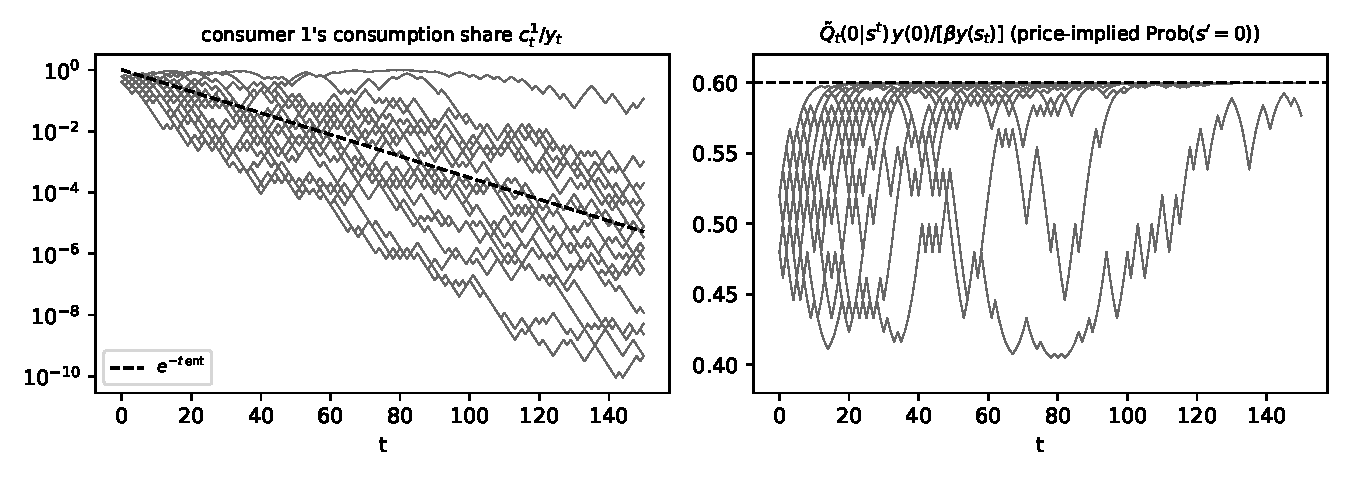
\includegraphics[width=0.9\textwidth]{figures/ch8_22.pdf}\\
{\small Figure S8.1.  Twenty simulated paths ($\alpha_1=.4$, $\alpha_2=\tilde\alpha=.6$, $\lambda=.5$).  Left: consumer 1's consumption share against $e^{-t\,\mathrm{ent}}$.  Right: the
probability of $s'=0$ implied by Arrow prices, which converges to the truth.}
\end{center}
\end{ex}

%%---------------------------------------------------------------------------
\begin{ex}{8.23}{Recursive version of the Pareto problem}
\textbf{(a)--(c)}  The recursive Pareto problem is the Bellman equation of the exercise, with consumer 1's promised value $v$ as the state and $(c_s,w_s)$ as the controls.  Each consumer's expected utility is computed with his own probabilities: consumer 2's value $P(v)$ with $\Pi^2$, and the
promise-keeping constraint for consumer 1 with $\Pi^1$.

\textbf{(d)}  With multiplier $\theta\ge0$ on promise keeping, the Lagrangian is
$\sum_s\Pi^2_s[u_2(1-c_s)+\beta P(w_s)]+\theta\bigl(\sum_s\Pi^1_s[u_1(c_s)+\beta w_s]-v\bigr)$.  The first-order conditions and the envelope condition are
\[
  \Pi^2_su_2'(1-c_s)=\theta\,\Pi^1_su_1'(c_s),\qquad \Pi^2_sP'(w_s)+\theta\,\Pi^1_s=0,\qquad P'(v)=-\theta .
\]
Hence
\[
  \frac{u_2'(1-c_s)}{u_1'(c_s)}=-P'(v)\,\frac{\Pi^1_s}{\Pi^2_s},\qquad P'(w_s)=P'(v)\,\frac{\Pi^1_s}{\Pi^2_s}.
\]

\textbf{(e)}  The left side of the first condition is increasing in $c_s$, since $u_1'$ falls and $u_2'(1-c_s)$ rises as $c_s$ rises.  So $c_s$ is increasing in $\Pi^1_s/\Pi^2_s$.  In the
second condition, $P'(v)<0$, so a ratio above 1 makes $P'(w_s)$ more negative.  Because $P$ is concave, that means $w_s>v$; a ratio below 1 gives $w_s<v$.  Thus in states that consumer 1
considers relatively more likely, he gets both more consumption now and a higher continuation value, and in the other states less of both.  With common beliefs the ratio is 1,
$w_s=v$ and $c_s$ is constant: the result of Section 8.12.

\textbf{(f)}  The relative Pareto weight $-P'(v_t)$ evolves as $-P'(v_{t+1})=-P'(v_t)\,\Pi^1(s_{t+1})/\Pi^2(s_{t+1})$, so
\[
  -P'(v_t)=-P'(v_0)\prod_{\tau\le t}\frac{\Pi^1(s_\tau)}{\Pi^2(s_\tau)}=-P'(v_0)\,\frac{\pi^1_t(s^t)}{\pi^2_t(s^t)} .
\]
This is exactly the continuation Pareto weight $\lambda^t_i(s^t)\propto\pi^i_t(s^t)\lambda_i$ of Appendix B, now carried as a state variable (the promised value).  If consumer 2's beliefs
are closer to the truth, the likelihood ratio $\pi^1_t/\pi^2_t$ goes to zero almost surely, at the exponential rate of Exercise 8.22.  Consumer 1's weight then vanishes, his
promised value drifts down to the bottom of the admissible set, and his consumption goes to zero.  The recursive formulation shows the market-selection result of Appendix B
through the drift of continuation values.
\end{ex}

%%---------------------------------------------------------------------------
\begin{ex}{8.24}{Recovering probabilities from prices}
\textbf{(a)}  \bk{(8.10.3)} says $Q_h(j\given i)=\sum_kQ(k\given i)Q_{h-1}(j\given k)$, which is the $(i,j)$ element of the matrix product $QQ_{h-1}$.  Hence $Q_h=Q^h$.

\textbf{(b)}  Take $i=1$.  The first row of $Q_2=Q^2$ is
\[
  (Q^2)_{11}=Q_{11}^2+Q_{12}Q_{21},\qquad (Q^2)_{12}=Q_{11}Q_{12}+Q_{12}Q_{22}.
\]
If $Q_{12}>0$, these give the second row: $Q_{21}=[(Q^2)_{11}-Q_{11}^2]/Q_{12}$ and $Q_{22}=(Q^2)_{12}/Q_{12}-Q_{11}$.  (Row 2 of the data gives row 1 symmetrically.)

\textbf{(c)}  Consumption equals the endowment, so the Euler equation gives
\[
  Q_{ij}=\beta P_{ij}\Bigl(\frac{c_j}{c_i}\Bigr)^{-\gamma},\qquad\text{i.e.}\qquad Q=\beta D^{-1}PD,\quad D=\diag(c_1^{-\gamma},c_2^{-\gamma}).
\]

\textbf{(d)}  Let $x=(c_2/c_1)^{-\gamma}$.  Then $Q_{11}=\beta P_{11}$, $Q_{12}=\beta P_{12}x$, $Q_{21}=\beta P_{21}/x$ and $Q_{22}=\beta P_{22}$.  Because each row of $P$ sums to one,
$\beta=Q_{11}+Q_{12}/x=Q_{21}x+Q_{22}$, which gives the quadratic
\[
  Q_{21}x^2+(Q_{22}-Q_{11})x-Q_{12}=0 .
\]
The product of its roots is $-Q_{12}/Q_{21}<0$, so it has exactly one positive root.  That root gives $x$, then $\beta=Q_{11}+Q_{12}/x$, $P_{11}=Q_{11}/\beta$ and $P_{22}=Q_{22}/\beta$.
Only the combination $x=(c_2/c_1)^{-\gamma}$ is identified, not $\gamma$ itself (unless the consumption ratio is observed).

This is Ross's recovery theorem.  Since $Q=\beta D^{-1}PD$ and $P\mathbf 1=\mathbf 1$, we have $Q(D^{-1}\mathbf 1)=\beta D^{-1}\mathbf 1$.  So $\beta$ is the Perron root of the positive matrix $Q$,
and its positive eigenvector $z=(c_1^\gamma,c_2^\gamma)$ gives $D$, hence $P=\beta^{-1}DQD^{-1}$.  With $\beta=.96$, $\gamma=2$, $P=\bigl[\begin{smallmatrix}.8&.2\\.15&.85\end{smallmatrix}\bigr]$ and $c=(1,1.2)$,
\texttt{ch8.py} recovers row 2 of $Q$ from row 1 of $Q$ and $Q^2$.  From $Q$ it recovers $\beta=.96$, $P_{11}=.8$, $P_{22}=.85$ and $x=1.2^{-2}=.69444$ exactly.  The Perron root is $.96$ and the
eigenvector ratio is $1.44=1.2^2$.
\end{ex}

%%---------------------------------------------------------------------------
\begin{ex}{8.25}{Recovering probabilities from prices, II}
\textbf{(a)--(b)}  Exactly as in Exercise 8.24(a)--(b).

\textbf{(c)}  $c_{t+1}/c_t=\lambda(s_{t+1})$, so $Q_{ij}=\beta P_{ij}\lambda_j^{-\gamma}$: $Q=P\,\diag(z)$ with $z_j=\beta\lambda_j^{-\gamma}$.  The discount factor depends only on tomorrow's state.

\textbf{(d)}  Row sums of $P$ equal one, so $Q\,\diag(z)^{-1}\mathbf 1=\mathbf 1$, i.e.\ $(1/z_1,1/z_2)'=Q^{-1}\mathbf 1$.  Thus $Q$ reveals $z$, and then $P=Q\diag(z)^{-1}$: here the transition
probabilities \emph{are} identified.  But $\beta$ is not.  The two numbers $z_j=\beta\lambda_j^{-\gamma}$ involve three unknowns, $\beta,\lambda_1,\lambda_2$, and for any $\beta$ the growth rates
$\lambda_j=(\beta/z_j)^{1/\gamma}$ reproduce $Q$ exactly.  So even with $\gamma$ known, $\beta$ (and with it the pair $(\beta,P)$) cannot be inferred from $Q$ unless growth rates are observed.
\texttt{ch8.py} illustrates with $\beta=.96$, $\gamma=2$, $P$ as in 8.24 and $\lambda=(.98,1.03)$.  It recovers $P$ from $Q$ alone, and $(\beta,\lambda)=(.90;\ .9489,.9973)$,
$(.96;\ .98,1.03)$ and $(.99;\ .9952,1.0460)$ all generate the same $Q$.

\emph{Why Ross's method fails here.}  Applying the Perron--Frobenius recovery of Exercise 8.24 to this $Q$ gives $\hat\beta=.9498$ and
$\hat P=\bigl[\begin{smallmatrix}.842&.158\\.190&.810\end{smallmatrix}\bigr]$, both wrong.  In a growth economy the stochastic discount factor $\beta(c_{t+1}/c_t)^{-\gamma}$ is not of the ratio form
$\beta d(s_{t+1})/d(s_t)$.  It has a permanent (martingale) component, and Perron--Frobenius recovers a ``long-term risk-neutral'' measure instead of the true probabilities
(Borovi\v{c}ka, Hansen and Scheinkman, 2016).
\end{ex}

%%---------------------------------------------------------------------------
\begin{ex}{8.26}{Recovering probabilities from prices, III}
\textbf{(a)}  $m_{t,t+h}=\beta^h(c_{t+h}/c_t)^{-\gamma}$: the price of any claim to $d_{t+h}$ is $E_t[m_{t,t+h}d_{t+h}]$.  Markets are complete (one-period Arrow securities in every state, traded
every period), so state prices are unique, and so is the discount factor, $m=q/\pi$ state by state.

\textbf{(b)}  A bond pays 1 in every state, so $p^t_{t+h}=\sum_j(Q^h)_{s_t,j}=\beta^hE_t[(c_{t+h}/c_t)^{-\gamma}]$.

\textbf{(c)}  No.  Since $Q=\beta D^{-1}PD$ is similar to $\beta P$, its eigenvalues are $\beta$ and $\beta\rho$ with $\rho=P_{11}+P_{22}-1$.  By the Cayley--Hamilton theorem
$Q^2=e_1Q-e_2I$, where $e_1=\tr Q=\beta(P_{11}+P_{22})$ and $e_2=\det Q=\beta^2\rho$.  Hence the bond prices obey
\[
  p_{h+2}=e_1p_{h+1}-e_2p_h,\qquad p_0=1 .
\]
From $p_1,p_2,p_3$ one obtains $e_1$ and $e_2$, i.e.\ $\beta$ (the larger root of $z^2-e_1z+e_2=0$) and $\rho$.  Then $p_4$ is implied by the recursion and carries no new information.
The remaining datum is $p_1=\beta[P_{11}+(1-P_{11})r]$ (for $s_t=1$), with $r=(c(2)/c(1))^{-\gamma}$.  That is one equation in the two unknowns $P_{11}$ and $r$, with $P_{22}=1+\rho-P_{11}$.
So $\beta$ and $P_{11}+P_{22}$ are identified, but $P_{11}$, $P_{22}$ and the marginal-utility ratio are not separately.  Example (\texttt{ch8.py}): $(\beta,P_{11},P_{22},r)=(.95,.8,.7,.7)$ and $(.95,.7,.8,.8)$
give identical prices $p_1,\dots,p_4=(.893,\ .821275,\ .767351,\ .722874)$.  The recursion recovers the roots $(.95,.475)$ and predicts $p_4$ exactly.  Bonds span only the conditional
expectation of the discount factor, not its distribution across states, and that is what the Arrow prices of Exercise 8.24 add.
\end{ex}

%%---------------------------------------------------------------------------
\begin{ex}{8.27}{Corners}
\textbf{(a)}  The problem separates by date and history: maximize $\alpha c^1+(1-\alpha)\ln c^2$ subject to $c^1+c^2\le Y(s)\equiv y^1(s)+y^2(s)$ and $c^i\ge0$.  In an interior optimum
$\alpha=(1-\alpha)/c^2$, so the log consumer eats the constant amount $(1-\alpha)/\alpha$ and the risk-neutral consumer absorbs all fluctuations.  Hence
\[
  c^2(s)=\min\Bigl\{\frac{1-\alpha}{\alpha},\,Y(s)\Bigr\},\qquad c^1(s)=\max\Bigl\{0,\,Y(s)-\frac{1-\alpha}{\alpha}\Bigr\}.
\]
The constraint $c^2\ge0$ never binds, because $u_2'(0)=\infty$.  The constraint $c^1\ge0$ binds in states where the aggregate endowment falls short of $(1-\alpha)/\alpha$.  There type 2
consumes the whole aggregate endowment, $c^2=Y(s)$, and consumption fluctuates with $Y$ because the risk-neutral consumer cannot absorb the shortfall.

\textbf{(b)}  Arrow prices $Q(s'\given s)$, consumption $c^i(s^t)\ge0$ and holdings $a^i_{t+1}(s')$ such that each type maximizes $V_i$ subject to
$c^i_t+\sum_{s'}Q(s'\given s_t)a^i_{t+1}(s')\le y^i(s_t)+a^i_t$, $a^i_0=0$ and natural debt limits, and markets clear: $\sum_ic^i_t=Y(s_t)$ and $\sum_ia^i_{t+1}(s')=0$.

\textbf{(c)}  \emph{Assumption 1 (interior).}  Type 1's first-order condition with constant marginal utility gives risk-neutral prices, $Q(s'\given s)=\beta P(s,s')$.  Type 2's Euler
equation $Q(s'\given s)=\beta P(s,s')c^2(s)/c^2(s')$ then forces constant consumption $\bar c^2$.  His budget fixes it at the annuity value of his endowment at these prices,
\[
  \bar c^2=(1-\beta)\bigl[(I-\beta P)^{-1}y^2\bigr](s_0),\qquad c^1(s)=Y(s)-\bar c^2 .
\]
This is valid if and only if $\bar c^2\le\min_sY(s)$.  Holdings are $a^i(s)=[(I-Q)^{-1}(c^i-y^i)](s)$.  In the example of \texttt{ch8.py}, $\lambda=.3$, $\delta=.4$, $\beta=.95$,
$y^1=(1,1)$, $y^2=(0,a)$ and $s_0=\bar s_1$.  With $a=.5$: $\bar c^2=.2588$ and $c^1=(.7412,1.2412)$.  With $a=1.5$: $\bar c^2=.7763$.  The assumption holds for $a\le a^*=1.9323$.

\emph{Assumption 2 (a corner).}  Suppose type 1's constraint binds in the low-endowment state $\ell$ and not in the high state $h$.  Then $c^1(\ell)=0$ and $c^2(\ell)=Y(\ell)$.  Type 1's first-order
conditions, $\beta^t\pi_t\le\mu_1q^0_t$ with equality where $c^1>0$, combined with type 2's $\beta^t\pi_t/c^2_t=\mu_2q^0_t$, give $c^2_t\le\mu_1/\mu_2\equiv k$, with equality where $c^1>0$.
So $c^2(h)=k$, and prices are set by type 2:
\[
  Q(s'\given s)=\beta P(s,s')\,\frac{c^2(s)}{c^2(s')}\qquad\bigl(\ge\beta P(s,s')\text{ when }s'=\ell\bigr).
\]
Type 2's budget pins down $k$.  With log utility it reads $\sum_t\beta^tE_0[y^2_t/c^2_t]=1/(1-\beta)$.  For $a=4$: $c^2=(1,2.0700)$, $c^1=(0,2.9300)$, and
$Q=\bigl[\begin{smallmatrix}.2850&.3213\\1.1799&.3800\end{smallmatrix}\bigr]$.  Consumption in the low state is scarce, so its Arrow price from the high state exceeds 1.  Type 1's shadow value of
wealth in the low state is $k/c^2(\ell)=2.07>1$; he would like to consume a negative amount there.  (If ``always binds'' is read as binding at every date, type 1 would consume nothing
ever, which is an equilibrium only if he owns nothing, $y^1\equiv0$.  Then $c^2=Y$ and prices are $Q=\beta P(s,s')Y(s)/Y(s')$.)  This is the decentralized counterpart of the corner
in (a), with $(1-\alpha)/\alpha=k$ equal to the ratio of the consumers' marginal utilities of wealth.
\end{ex}

%%---------------------------------------------------------------------------
\begin{ex}{8.28}{Recovering probabilities from prices, IV}
\textbf{(a)}  As in Exercise 8.24: prices $Q^{(1)}_{ij}$ and a consumption plan such that the consumer maximizes expected utility subject to the sequential budget constraints, and
markets clear, $c_t=y(s_t)$ with zero asset holdings.  Adding two-period securities (part (c)) adds prices $Q^{(2)}_{ij}$ and the corresponding holdings.

\textbf{(b)}  With $x=(\bar y_2/\bar y_1)^{-\gamma}$,
\[
  Q^{(1)}=\begin{bmatrix}\beta\lambda&\beta(1-\lambda)x\\ \beta(1-\delta)/x&\beta\delta\end{bmatrix}.
\]

\textbf{(c)}  By no arbitrage, $Q^{(2)}=(Q^{(1)})^2$:
\[
  Q^{(2)}=\beta^2\begin{bmatrix}\lambda^2+(1-\lambda)(1-\delta)&x(1-\lambda)(\lambda+\delta)\\ x^{-1}(1-\delta)(\lambda+\delta)&(1-\delta)(1-\lambda)+\delta^2\end{bmatrix}.
\]

\textbf{(d)}  The four numbers are today's prices of consumption in each state one and two periods ahead.  Each is a probability times a discount factor times a marginal-utility
ratio: $Q^{(h)}(1,j)=\beta^h\Prob(s_{t+h}=j\given s_t=1)\,(\bar y_j/\bar y_1)^{-\gamma}$.  Yes, $\lambda$, $\delta$ and $\beta$ can be inferred.  By Exercise 8.24(b), the first row of
$Q^{(1)}$ and $Q^{(2)}$ gives the second row of $Q^{(1)}$, and by Exercise 8.24(d) the full $Q^{(1)}$ gives $\beta$, $\lambda$, $\delta$ and $x$.  What cannot be inferred is $\gamma$ separately
from the endowment ratio: only $x=(\bar y_2/\bar y_1)^{-\gamma}$ is identified.  Check (\texttt{ch8.py}): with $(\lambda,\delta,\beta,\gamma,\bar y_1,\bar y_2)=(.7,.6,.95,3,1,1.1)$, the observed row is
$(.665,\ .214125)$ and $(.550525,\ .264444)$, and the procedure returns $\beta=.95$, $\lambda=.7$, $\delta=.6$ and $x=.751315$ exactly.  The argument uses the stationarity of the level
economy.  In a growth economy the same data would not reveal $\beta$ (Exercise 8.25).
\end{ex}

%% ===========================================================================
%% Chapter 9. Overlapping Generations
%% ===========================================================================
\solchapter{9}{Overlapping Generations}

\begin{center}
\begin{minipage}{0.86\textwidth}
\small
Solutions to all 13 exercises of Chapter 9 of Ljungqvist and Sargent, \emph{Recursive Macroeconomic Theory} (4th edition, 2018).  The exercises are mostly analytical.
\texttt{code/ch9.py} checks every closed form numerically (Euler equations, difference equations for real balances, the tree economy of 9.3, the Laffer curves of 9.10 and
9.13, credit controls, the Grandmont--Hall scheme and forced saving) and draws the figures.
\end{minipage}
\end{center}

\bigskip
\hrule
\bigskip

Throughout, $R_t$ is the gross real return between $t$ and $t+1$ (on currency, $R_t=p_t/p_{t+1}$), and $m_t$ denotes real balances per young person.  With $\ln c^t_t+\ln c^t_{t+1}$ and
endowment $(w_1,w_2)$, a young person saving $s$ at return $R$ solves $\max\ln(w_1-s)+\ln(w_2+Rs)$.  The first-order condition $w_2+Rs=R(w_1-s)$ gives the saving function
\[
  s(R)=\tfrac12\bigl(w_1-w_2/R\bigr),
\]
which is positive if and only if $R>w_2/w_1$, the autarky (no-trade) interest rate.

%%---------------------------------------------------------------------------
\begin{ex}{9.1}{Equilibria with valued fiat currency}
\textbf{(a)}  The first-order condition $u'(w_1-s)=Ru'(w_2+Rs)$ reads $(w_1-s)^{-\gamma}=R(w_2+Rs)^{-\gamma}$, i.e.\ $w_2+Rs=R^{1/\gamma}(w_1-s)$, so
\[
  s(R)=\frac{R^{1/\gamma}w_1-w_2}{R^{1/\gamma}+R},\qquad s(R)>0\iff R>R_{aut}\equiv(w_2/w_1)^\gamma .
\]
For $\gamma=1$ this is $s(R)=\frac12(w_1-w_2/R)$.  For $\gamma\le1$, $s$ is increasing in $R$; for $\gamma>1$ the income effect can make it bend backward at high returns.

\textbf{(b)}  A price sequence $\{p_t\}_{t\ge1}$ with $0<p_t<\infty$ and an allocation such that: each young agent born at $t\ge1$ maximizes utility given the return $R_t=p_t/p_{t+1}$ on
currency; the initial old consume $c^0_1=w_2+M/(Np_1)$; and the currency market clears, $\frac{M}{Np_t}=s\bigl(p_t/p_{t+1}\bigr)$ for all $t\ge1$.  Equivalently, with $m_t=M/(Np_t)$,
\[
  m_t=s(R_t),\qquad m_{t+1}=R_tm_t .
\]

\textbf{(c)}  An equilibrium with valued currency in which $p_t=\bar p$ is constant (so $R_t=1$ and $m_t=\bar m$).

\textbf{(d)}  With $R=1$: $\bar m=s(1)=\frac12(w_1-w_2)>0$, so
\[
  \bar p=\frac{2M}{N(w_1-w_2)},\qquad c^t_t=c^t_{t+1}=\tfrac12(w_1+w_2).
\]
This holds for every $\gamma$, since $R=1$ makes the agent equalize consumption.

\textbf{(e)}  A continuum.  The equilibrium conditions form a first-order difference equation in real balances: $m_t$ determines $R_t$ through $s(R_t)=m_t$, and then $m_{t+1}=R_tm_t$.  Any
$m_1\in(0,\bar m]$ (equivalently $p_1\ge\bar p$) starts an equilibrium.  With $s$ increasing, $m_1<\bar m$ gives $R_1<1$, so $m_2<m_1$, and so on: $m_t$ decreases to 0 and the value
of currency vanishes.  $m_1>\bar m$ gives $R_t>1$ and $m_t$ grows until saving would have to exceed $w_1$, which is impossible.  So the equilibria are indexed by $p_1\in[\bar p,\infty)$: the
stationary one and a continuum of nonstationary ones.  For $\gamma=1$ the chapter's (9.4.8) gives them in closed form, $p_t=\bar p+c\,(w_1/w_2)^t$ with $c\ge0$.  (For large $\gamma$ the
saving function can bend backward, as it does in \texttt{ch9.py} for $\gamma=5$.  Then $s(R_t)=m_t$ can have two solutions, and there are even more equilibria.)

\textbf{(f)}  In every nonstationary equilibrium $m_t\to0$.  Since $m_t=s(R_t)$ and $s$ is continuous with $s(R)\to0$ only as $R\downarrow R_{aut}$,
\[
  \lim_{t\to\infty}R_t=R_{aut}=(w_2/w_1)^\gamma<1 .
\]
The rate of return on currency converges to the autarky interest rate, and inflation to $(w_1/w_2)^\gamma$.  The economy approaches the nonmonetary equilibrium, where the young's
marginal rate of substitution at the endowment, $u'(w_1)/u'(w_2)=(w_2/w_1)^\gamma$, is the (shadow) interest rate.  \texttt{ch9.py} iterates the difference equation from
$m_1=\bar m/2$ with $(w_1,w_2)=(2,1)$ and finds $R_{60}=.7071,.5000,.2500,.0313$ for $\gamma=.5,1,2,5$, equal to $(1/2)^\gamma$.
\end{ex}

%%---------------------------------------------------------------------------
\begin{ex}{9.2}{Heterogeneous endowments and valued currency}
\textbf{(a)}  Type 1, endowed with $(w_1,0)$: $\max\ln(w_1-s)+\ln(Rs)$ gives $s_1=w_1/2$, independent of $R$.  Type 2, endowed with $(0,w_2)$: $\max\ln(-s)+\ln(w_2+Rs)$ gives
$s_2(R)=-w_2/(2R)$, so type 2 borrows $w_2/(2R)$ and repays $w_2/2$.

\textbf{(b)}  Without valued currency the only trades are loans within a generation.  The loan market clears when $\frac N2s_1+\frac N2s_2(R_t)=0$, so
\[
  R_t=w_2/w_1\quad\text{for all }t,
\]
and this equilibrium is unique.  Each young person of either type consumes $w_1/2$ when young and $w_2/2$ when old.  The initial old consume their endowments ($w_2$ or $0$).

\textbf{(c)}  Prices $0<p_t<\infty$ and an allocation with each young person optimizing at $R_t=p_t/p_{t+1}$, where the young's net saving equals the real value of the currency stock:
$\frac N2\cdot\frac{w_1}2-\frac N2\cdot\frac{w_2}{2R_t}=\frac{NM}{p_t}$ for $t\ge1$.

\textbf{(d)}  Dividing by $N/4$, $4M=w_1p_t-w_2p_{t+1}$, i.e.\ $p_{t+1}=\frac{w_1}{w_2}p_t-\frac{4M}{w_2}$.  The general solution is
\[
  p_t=\bar p+c\Bigl(\frac{w_1}{w_2}\Bigr)^t,\qquad \bar p=\frac{4M}{w_1-w_2},
\]
and $c\ge0$ is required for $p_t>0$ at all $t$, since $w_1/w_2>1$.  So the equilibria with valued currency are indexed by $c\ge0$ (equivalently $p_1\ge\bar p$).  For $c>0$ the price level
explodes, real balances go to zero, and $R_t=p_t/p_{t+1}$ falls monotonically to $w_2/w_1$, the nonmonetary interest rate (Figure S9.1).

\textbf{(e)}  A constant $p_t$ requires $c=0$, so $\bar p=4M/(w_1-w_2)$ is the unique stationary equilibrium, with $R=1$.

\textbf{(f)}  The equilibria are not Pareto ranked.  A lender's utility $\ln(w_1/2)+\ln(R_tw_1/2)$ rises with $R_t$, while a borrower's utility $\ln\frac{w_2}{2R_t}+\ln\frac{w_2}2$ falls with $R_t$.
Along each path, $R_t$ is highest in the stationary equilibrium ($R_t=1$) and decreasing in $c$.  So lenders and the initial old, whose consumption $M/p_1$ is larger when $p_1$ is
smaller, prefer the stationary equilibrium, while borrowers prefer equilibria with lower interest rates.  (With $(w_1,w_2)=(2,1)$: generation 1's lenders get utility $0$ at $c=0$ and
$-.182$ at $c=.5$; its borrowers get $-1.386$ and $-1.204$.)
\begin{center}
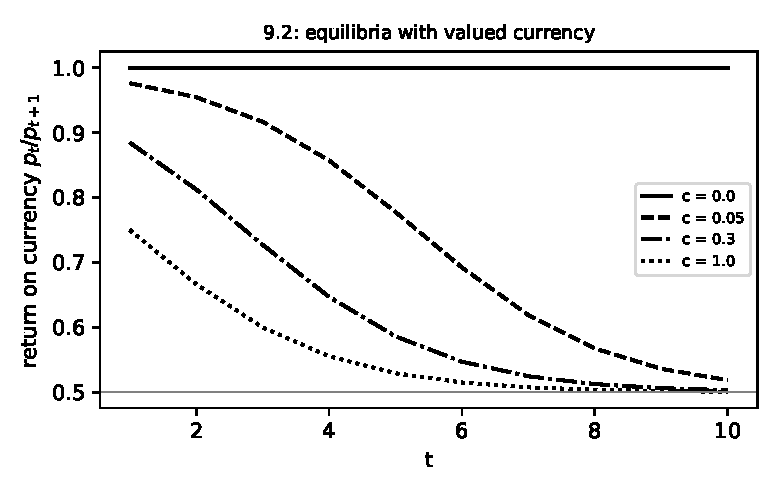
\includegraphics[width=0.55\textwidth]{figures/ch9_02.pdf}\\
{\small Figure S9.1.  Exercise 9.2 with $(w_1,w_2)=(2,1)$: the return on currency in the equilibria $p_t=\bar p+c(w_1/w_2)^t$.  Only $c=0$ is stationary; the others converge to
the nonmonetary rate $w_2/w_1$.}
\end{center}
\end{ex}

%%---------------------------------------------------------------------------
\begin{ex}{9.3}{A tree with a tiny dividend}
Let $q_t$ be the ex-dividend price of the tree per young person (normalize $N=1$).  Whoever buys it at $t$ receives $q_{t+1}+d$ at $t+1$.

\textbf{(a)}  There is none.  Suppose currency is valued at every date.  Then currency and the tree must earn the same return, $R_t=p_t/p_{t+1}=(q_{t+1}+d)/q_t$.  Real balances obey
$m_{t+1}=R_tm_t$, so $R_1R_2\cdots R_{t-1}=m_t/m_1\le w_1/m_1$, because saving cannot exceed $w_1$.  Solving the tree's pricing equation forward,
\[
  q_1\ \ge\ \sum_{t=1}^T\frac{d}{R_1\cdots R_t}\ \ge\ T\,d\,\frac{m_1}{w_1}\ \longrightarrow\ \infty ,
\]
which contradicts $q_1\le s(R_1)<w_1$.  When currency has a nonnegative real rate of return in the long run, the tree's dividend stream is worth infinitely much.  So any
positive dividend eliminates all equilibria with valued fiat currency.

\textbf{(b)}  The tree is the only asset: $s(R_t)=q_t$ and $R_tq_t=q_{t+1}+d$.  A stationary equilibrium has $q=s(R)$ and $q(R-1)=d$, i.e.
\[
  s(R)(R-1)=d,\qquad R>1 .
\]
The left side is 0 at $R=1$ and increases in $R$ (as long as $s$ does), so there is a unique solution $R^*>1$, with $q^*=s(R^*)$.  It is also the only equilibrium.  Write the dynamics as
$q_{t+1}=R(q_t)q_t-d$, where $R(q)=s^{-1}(q)$ is increasing.  Then $q_{t+1}-q_t=(R(q_t)-1)q_t-d$ is positive for $q_t>q^*$ and negative for $q_t<q^*$.  A path that starts above $q^*$ rises
until the young cannot afford the tree, and one that starts below falls until the tree's price would be negative.

\textbf{(c)}  With $w_1=10$, $w_2=5$, $d=10^{-6}$ and log utility (the exercise leaves $\gamma$ open; we take $\gamma=1$): $s(R)=5-2.5/R$, and $s(R)(R-1)=d$ gives
$R^*=1+4.0\times10^{-7}$ and $q^*=2.500001$.  \texttt{ch9.py} starts the tree's price $10^{-3}$ above or below $q^*$ and finds that it leaves the feasible range after 11 and 32 periods.
The tree, with an almost worthless dividend, is priced like fiat money in the stationary monetary equilibrium of Exercise 9.1 ($\bar m=2.5$), and the allocation is essentially that
equilibrium's.  But whereas Exercise 9.1 has a continuum of monetary equilibria plus the nonmonetary one, the tiny dividend selects a single equilibrium, the stationary one.
\end{ex}

%%---------------------------------------------------------------------------
\begin{ex}{9.4}{Population growth}
\textbf{(a)}  All young people are identical, and the old cannot repay loans.  So there is no trade: each person consumes the endowment $(w_1,w_2)$, and the (shadow) interest rate is
the marginal rate of substitution at the endowment, $R_{aut}=w_2/w_1$.

\textbf{(b)}  In a stationary equilibrium real balances per young person are constant, $M/(N(t)p_t)=\bar m$, so total real balances grow with the population.  Then
$p_t/p_{t+1}=N(t+1)/N(t)=n$: currency earns the population growth rate.  Hence $\bar m=s(n)=\frac12(w_1-w_2/n)>0$ (since $n\ge1>w_2/w_1$) and
\[
  p_t=\frac{M}{N(t)\,s(n)}=\frac{2M}{N(t)(w_1-w_2/n)},\qquad c^t_t=\tfrac12\Bigl(w_1+\frac{w_2}{n}\Bigr),\qquad c^t_{t+1}=\tfrac12(nw_1+w_2).
\]
The price level falls at rate $n$.  Currency earns the ``biological'' rate of return $R=n$, which delivers the golden-rule allocation (the best stationary allocation, given the
resource constraint $c^t_t+c^{t-1}_t/n=w_1+w_2/n$).
\end{ex}

%%---------------------------------------------------------------------------
\begin{ex}{9.5}{Population growth and all monetary equilibria}
\textbf{(a)}  An equilibrium without valued currency is an allocation and interest rates at which the young optimize and loans clear (and $1/p_t=0$).  All young are identical, so it is
autarky, with interest rate $R_{aut}=w_2/w_1$.

\textbf{(b)}  Prices $0<p_t<\infty$ with $N(t)s(R_t)=N(0)/p_t$ (the total currency stock is $H=N(0)$) and $R_t=p_t/p_{t+1}$.

\textbf{(c)}  Let $m_t=H/(N(t)p_t)$.  Then $m_{t+1}=R_tm_t/n$, so $R_t=nm_{t+1}/m_t$, and $m_t=\frac12\bigl(w_1-\frac{w_2m_t}{nm_{t+1}}\bigr)$.  In terms of $x_t=1/m_t$ this equation is linear:
\[
  x_{t+1}=\frac{nw_1}{w_2}\,x_t-\frac{2n}{w_2},\qquad\text{so}\qquad x_t=x^*+c\Bigl(\frac{nw_1}{w_2}\Bigr)^t,\quad x^*=\frac1{m^*},\quad m^*=\tfrac12\Bigl(w_1-\frac{w_2}n\Bigr).
\]
Valued currency requires $m_t>0$ for all $t$.
\begin{itemize}
  \item If $n\le w_2/w_1$, then $m^*\le0$.  No equilibrium with valued currency exists: autarky already offers a return $w_2/w_1\ge n$, at least what currency could pay.
  \item If $n>w_2/w_1$, then $nw_1/w_2>1$ and the equilibria are indexed by $c\ge0$.  $c=0$ is the stationary one ($m_t=m^*$, $R_t=n$), and $c>0$ gives $x_t\to\infty$, i.e.\ $m_t\to0$.  ($c<0$
  would make $m_t$ negative eventually.)
\end{itemize}

\textbf{(d)}  In the stationary equilibrium $R_t=n$.  In the others $R_t=n\,x_t/x_{t+1}\to n\cdot\frac{w_2}{nw_1}=w_2/w_1$, the autarky rate of (a): the value of currency vanishes and the economy
converges to autarky.  (\texttt{ch9.py}: with $(w_1,w_2)=(2,1)$ and $n=1.2$, $R_t$ falls from $.993$ to $.5000$.)

\textbf{(e)}  Yes.  A young person's utility increases with the return on saving ($s>0$ in any monetary equilibrium), and $R_t=n\frac{x^*+c\lambda^t}{x^*+c\lambda^{t+1}}$, with
$\lambda=nw_1/w_2>1$, is decreasing in $c$ at every $t$.  The initial old consume $w_2+1/p_1$, which is also decreasing in $c$.  So every generation prefers smaller $c$: the equilibria are
Pareto ranked, the stationary one ($c=0$) is best, and autarky, the limit $c\to\infty$, is worst.  The difference from Exercise 9.2 is that here all young people are lenders.
\end{ex}

%%---------------------------------------------------------------------------
\begin{ex}{9.6}{Exchange rate determinacy}
\emph{Preliminaries.}  A poor young person saves $\alpha/2$ whatever the return (log utility, no endowment when old), and can save only in currency.  World real money demand is
therefore constant at $2N\cdot\alpha/2=N\alpha$.  The rich save $(\beta-T_i/N)/2$ in storage or bonds at $R$; currency, which returns less than $R$, is dominated for them.

\textbf{(a)}  Price levels $0<p_i(t)<\infty$, government policies satisfying the budget constraints, and an allocation such that: the poor choose currency portfolios and the rich
choose storage and bonds optimally; the goods markets clear; and the currency markets clear, $\frac{H_1(t)}{p_1(t)}+\frac{H_2(t)}{p_2(t)}=N\alpha$ together with a split of this demand across
the currencies that poor people are willing to hold.

\textbf{(b)}  If both currencies are valued, poor people hold both, which they do only if the returns are equal: $\frac{p_1(t)}{p_1(t+1)}=\frac{p_2(t)}{p_2(t+1)}$.  If one return were higher, nobody
would hold the other currency.  Rearranging, $e_t=p_1(t)/p_2(t)=p_1(t+1)/p_2(t+1)=e_{t+1}$: the exchange rate is constant.

\textbf{(c)}  Let $m_i(t)=H_i(t)/p_i(t)$ and $\sigma_i=G_i-T_i$.  With $B_i=0$, each government finances $\sigma_i$ by seigniorage:
$m_i(t)-R_m(t-1)m_i(t-1)=\sigma_i$ for $t\ge2$, and $m_i(1)=\sigma_i+H_i(0)/p_i(1)$, where $R_m$ is the common return on currency.  Adding across countries and using $m_1+m_2=N\alpha$ gives
$R_m=1-(\sigma_1+\sigma_2)/(N\alpha)$ for all $t$.  At $t=1$ the two unknown price levels must satisfy only one equation,
\[
  \frac{H_1(0)}{p_1(1)}+\frac{H_2(0)}{p_2(1)}=N\alpha-\sigma_1-\sigma_2 .
\]
Every exchange rate $e=p_1(1)/p_2(1)$ in a nonempty interval (with both terms positive) is consistent with equilibrium, and then stays constant by (b).  Governments set their policies
in real terms, and nothing pins down how the fixed world demand for real balances is divided between the two perfectly substitutable currencies.  This is Kareken and Wallace's
indeterminacy.

\textbf{(d)}  For $t\ge2$ the budget reads $G_i+RB_i(1)=B_i(1)+T_i$ (no money creation), a restriction on the constants.  At $t=1$ it reads
$G_i=B_i(1)+[H_i(1)-H_i(0)]/p_i(1)+T_i$, which gives
\[
  p_i(1)=\frac{H_i(1)-H_i(0)}{G_i-T_i-B_i(1)}
\]
(for $H_i(1)\ne H_i(0)$).  Each government's nominal injection must buy a given real amount of goods, which pins down its own price level.  So $e=p_1(1)/p_2(1)$ is determinate.  With
constant money stocks and equal returns, $m_1$ and $m_2$ are constant, so the price levels are constant as well.  An equilibrium exists only if these price levels also satisfy
$H_1(1)/p_1(1)+H_2(1)/p_2(1)=N\alpha$.

\textbf{(e)}  The exercise does not say how country 2 finances the residual $G_2+(R-1)B_2(1)-T_2(t)$.  If country 2 financed it by printing money at a given real rate, both governments
would be setting real seigniorage, and we would be back in case (c), with an indeterminate exchange rate.  The claim holds under the reading that parallels (d): country 2 fixes its
money stock after an initial issue at $t=1$, $H_2(t)=H_2(1)$, and lets taxes absorb the residual.  (Country 1 finances $G_1$ at $t=1$ with $B_1(1)=0$ and a given tax.)  Then:
\begin{itemize}
  \item country 2's $t=1$ budget, $G_2=B_2(1)+[H_2(1)-H_2(0)]/p_2(1)+T_2(1)$, pins down $p_2(1)$ as in (d);
  \item the world money market gives $m_1(1)=N\alpha-H_2(1)/p_2(1)$;
  \item country 1's $t=1$ budget, $H_1(0)/p_1(1)=m_1(1)-(G_1-T_1(1))$, then pins down $p_1(1)$.
\end{itemize}
So $e=p_1(1)/p_2(1)$ is determinate, and it is constant thereafter by (b).  From $t=2$ on, $m_1(t)=s_1+R_m(t-1)m_1(t-1)$ and $R_m(t-1)=m_2(t)/m_2(t-1)$ determine the whole path.  One can show
$N\alpha-m_1(t)=(N\alpha-m_1(t-1))(1-s_1/(N\alpha))$: country 1's currency gradually takes over the world money demand, and currency pays $R_m=1-s_1/(N\alpha)$.  The general principle is that the
exchange rate is determinate when at least one government fixes a nominal quantity that its budget constraint ties to its price level.  With purely real policies, as in (c), it is not.
\end{ex}

%%---------------------------------------------------------------------------
\begin{ex}{9.7}{Credit controls}
Lenders save $y/2$ at any return.  Unconstrained borrowers borrow $y/(2R)$ and repay $y/2$.

\textbf{(a)}  Prices $1/p_t=0$ and a loan return $R_t$ such that each young person optimizes and the loan market clears.  Only lenders and borrowers of the same generation trade:
lenders lend to borrowers of their own generation.

\textbf{(b)}  Clearing requires $\frac N2\frac y2=\frac N2\frac y{2R}$, so $R=1$.  Everybody consumes $(y/2,y/2)$, and the initial old consume nothing.

\textbf{(c)}  Prices $0<p_t<\infty$ at which lenders are willing to hold both loans and currency, so $R_t=p_t/p_{t+1}$.  The young's net saving must equal the real value of the currency
stock:
\[
  \tfrac N2\cdot\tfrac y2-\tfrac N2\cdot\tfrac y{2R_t}=\frac{H(0)}{p_t}.
\]
The young lend to each other and buy the old's currency.

\textbf{(d)}  With $m_t=H(0)/(Np_t)>0$, the condition reads $m_t=\frac y4(1-1/R_t)$, which requires $R_t>1$.  Then $m_{t+1}=R_tm_t=m_t/(1-4m_t/y)>m_t$, so
$m_{t+1}-m_t=\frac{4m_t^2}{y-4m_t}\ge\frac{4m_1^2}{y}>0$.  Real balances rise by at least a fixed amount each period, so they eventually exceed $y/4$, the most the young could want to
hold.  (\texttt{ch9.py}: from $m_1=.01$ with $y=1$ this takes 24 periods.)  A constant price level would need $R=1$ and hence $m=0$.  So no equilibrium with valued currency exists.  At
$R=1$ intragenerational lending already absorbs all saving, and currency could only be valued at a return above 1, which feeds on itself.

\textbf{(e)}  Borrowers may promise at most $y/4$, and they want to promise $y/2$, so the limit binds: each borrows $y/(4R)$.  Clearing, $\frac y2=\frac y{4R}$, gives $R=\frac12$.  Lenders
consume $(y/2,y/4)$ and borrowers $(y/2,3y/4)$.

\textbf{(f)}  With a constant price level currency returns 1, so loans must return 1 too.  Borrowers still want to borrow $y/2$ at $R=1$ and are held to $y/4$.  Each lender therefore lends
$y/4$ and holds the other $y/4$ of saving in currency.  Real balances are $\frac N2\cdot\frac y4=\frac{H(0)}p$, so
\[
  p=\frac{8}{y}\,\frac{H(0)}N,\qquad q=\frac8y .
\]
Lenders consume $(y/2,y/2)$, borrowers $(y/4,3y/4)$, and each initial old person consumes $y/8$.  The return on loans is $R=1$.  The credit limit leaves an excess supply of loanable
funds, which currency absorbs.

\textbf{(g)}  Lenders get $(y/2,y/2)$ in both economies, so they are indifferent.  Borrowers are worse off in (f): $\ln\frac y4+\ln\frac{3y}4<2\ln\frac y2$ ($-1.674$ against $-1.386$ for $y=1$).
The initial old are better off in (f) ($y/8$ against $0$).  The credit control transfers resources from borrowers to the initial old by creating a demand for money.
\end{ex}

%%---------------------------------------------------------------------------
\begin{ex}{9.8}{Inside money and real bills}
\textbf{(a)}  Type 1 saves $y/2$, and type 2 borrows $Y/(2R)$.  Clearing, $N_1y/2=N_2Y/(2R)$, gives $1+r=N_2Y/(N_1y)$.

\textbf{(b)}  A constant price level makes currency return 1.  If currency is held, loans must also return 1, and then the young's net saving is $\frac{N_1y-N_2Y}2=H_0/p$.  But $1+r>1$ in
(a) means $N_2Y>N_1y$, so net saving would be negative, a contradiction.  With $N_2Y>N_1y$, the young as a group want to borrow at $R=1$: there is no demand for an outside asset.

\textbf{(c)}  If $N_2Y<N_1y$, set $R=1$ and $H_0/p=\frac{N_1y-N_2Y}2>0$, i.e.\ $q=\frac2{N_1y-N_2Y}$.  Everyone optimizes at $R=1$, loans and currency both pay 1, and markets clear.
The equilibrium is not Pareto superior to the nonmonetary one: type-2 people are borrowers, whose utility $\ln\frac Y{2R}+\ln\frac Y2$ is decreasing in $R$, and $R$ rises from
$N_2Y/(N_1y)<1$ to 1.  Lenders and the initial old gain, but borrowers lose.

\textbf{(d)}  (i) Guess $p(t)=\bar p$ and $R=1$.  The government's loans pay 1, so the $L_g$ it lent last period comes back as $L_g$ and is lent again.  Its budget balances, and
$M_I=L_g\bar p$ stays constant.  Type 1 holds currency, inside money and private loans, all paying 1.  Borrowers' demand $N_2Y/2$ is met by the government's $L_g$ plus private lending
$N_1y/2-(H_0+M_I)/\bar p$.  With $M_I/\bar p=L_g$, clearing reduces to $H_0/\bar p=(N_1y-N_2Y)/2$, the condition of (c).  So $\bar p=qH_0$ is again an equilibrium price level, with the
same allocation.

(ii) The inside money is backed one for one by private loans that earn the same return as money.  The government's purchase of $L_g$ loans displaces exactly $L_g$ of private lending,
and savers hold $L_g$ more inside money instead.  This is a pure swap of assets that savers regard as perfect substitutes, so aggregate demand for goods is unchanged.  This is the real
bills doctrine: money issued against sound private loans is not inflationary.

(iii) In many models, open-market operations exchange money for assets that are \emph{not} perfect substitutes for it.  Examples are government bonds backed by future taxes when money
pays a lower return, or settings where money is needed for transactions (cash-in-advance, reserve requirements).  Other operations change the government's net claims, so future
taxes or seigniorage must change.  Here there is no transaction role for money, money and loans pay the same return, and the government's loans fully back its liabilities.
\end{ex}

%%---------------------------------------------------------------------------
\begin{ex}{9.9}{Social security and the price level}
\textbf{(a)}  An equilibrium is $0<p_t<\infty$ with the young optimizing and $N s_t=H/p_t$.  With endowment $(y,0)$ the young save $y/2$ whatever the return, so
\[
  \frac H{p_t}=\frac{Ny}2\quad\Longrightarrow\quad p_t=\frac{2H}{Ny}\quad\text{for all }t .
\]
The market-clearing condition pins down every price level directly, so the equilibrium exists and is unique.  It is stationary, with $R=1$ and consumption $(y/2,y/2)$.

\textbf{(b)}  Now the effective endowment is $(y-\tau,\tau)$, and $s(R)=\frac12\bigl(y-\tau-\tau/R\bigr)$.  Valued currency needs $s>0$ at the returns it pays.  A stationary equilibrium
($R=1$) needs $s(1)=\frac12(y-2\tau)>0$, i.e.
\[
  \tau<\frac y2 .
\]
If $\tau\ge y/2$, social security already gives the old at least as much as the young, the autarky interest rate $\tau/(y-\tau)$ is at least 1, and currency cannot be valued: no
equilibrium with valued currency exists.

\textbf{(c)}  No.  With $\tau>0$ saving depends on the return, and $m_t=s(m_{t+1}/m_t)$ becomes $m_{t+1}=\tau m_t/(y-\tau-2m_t)$.  Its fixed point $\bar m=(y-2\tau)/2$ is unstable, and 0 is stable
(the slope there is $\tau/(y-\tau)<1$).  So every $m_1\in(0,\bar m]$ starts an equilibrium.  As in Exercise 9.1, there is a continuum of equilibria in which the value of currency goes to zero
and the return converges to $\tau/(y-\tau)$.

\textbf{(d)}  The stationary equilibrium is unique:
\[
  \bar p=\frac{H}{N\bar m}=\frac{2H}{N(y-2\tau)},
\]
which is increasing in $\tau$.  A larger social security system crowds out the demand for money, because the young need to save less for old age.  The price level rises (the value of
currency falls), and currency is worthless when $\tau\ge y/2$.
\end{ex}

%%---------------------------------------------------------------------------
\begin{ex}{9.10}{Seigniorage}
\textbf{(a)}  As in 9.8(a), $R=N_2\beta/(N_1\alpha)<1$.

\textbf{(b)}  No.  At the equilibrium every young person's marginal rate of substitution between youth and old age is $R<1$.  Let each young person, of either type, give $\varepsilon$ to the old
in every period.  Each person loses $\varepsilon$ when young and gains $\varepsilon$ when old.  The utility change is $\varepsilon[u'(c^{old})-u'(c^{young})]=\varepsilon u'(c^{young})(1/R-1)>0$ to first order, and
the initial old gain $\varepsilon$.  So there is a Pareto improvement.  (This is the Balasko--Shell criterion of Section 9.7.1: with interest rates below the growth rate, the allocation is
not optimal.)

\textbf{(c)}  Let $\mathcal M_t=H(t)/p(t)$ be real balances.  Then the return on currency is $R_t=p_t/p_{t+1}=\mathcal M_{t+1}/(z\mathcal M_t)$, and the young's net saving must equal
$\mathcal M_t$: $\frac{N_1\alpha}2-\frac{N_2\beta}{2R_t}=\mathcal M_t$.  Hence
\[
  \mathcal M_{t+1}=f(\mathcal M_t)\equiv\frac{N_2\beta z\,\mathcal M_t}{N_1\alpha-2\mathcal M_t}.
\]
The map $f$ is increasing and convex, with $f'(0)=N_2\beta z/(N_1\alpha)$.  Under the assumption $1/z>N_2\beta/(N_1\alpha)$, $f'(0)<1$, and $f$ has a positive fixed point
$\mathcal M^*=\frac12(N_1\alpha-N_2\beta z)$ with $f'(\mathcal M^*)>1$.  Every $\mathcal M_1\in(0,\mathcal M^*]$, i.e.\ every initial price level $p(1)\ge H(1)/\mathcal M^*$, starts an equilibrium, and for
$\mathcal M_1<\mathcal M^*$ real balances decline to zero.  That is a continuum.  (Starting above $\mathcal M^*$, real balances explode past $N_1\alpha/2$.)

\textbf{(d)}  The stationary equilibrium has
\[
  p(t)=\frac{2}{N_1\alpha-N_2\beta z}\,H(t),
\]
so the price level is proportional to the money stock and grows at rate $z$.  Currency and loans both return $1/z$.  Seigniorage is $G=\mathcal M^*(1-1/z)=\frac12(N_1\alpha-N_2\beta z)(1-1/z)$.

\textbf{(e)}  If $1/z<N_2\beta/(N_1\alpha)$, then $f(\mathcal M)/\mathcal M=\frac{N_2\beta z}{N_1\alpha-2\mathcal M}>1$ for every $\mathcal M>0$, so real balances grow from any positive start until they exceed
$N_1\alpha/2$: no equilibrium with valued currency exists.  Interpretation: at the money growth rate $z$, a stationary monetary equilibrium would pay $1/z$ on currency.  That is less than
the interest rate $N_2\beta/(N_1\alpha)$ that private loans pay even when nobody holds currency.  Currency is dominated in rate of return, so no one will hold it and the inflation tax
cannot be collected.

\textbf{(f)}  Write $a=N_1\alpha$, $b=N_2\beta$.  Then $G(z)=\frac12(a-bz)(1-1/z)=\frac12(a+b-bz-a/z)$ and $G'(z)=\frac12(a/z^2-b)$, so
\[
  z^*=\sqrt{a/b}=\sqrt{N_1\alpha/(N_2\beta)},\qquad G(z^*)=\tfrac12\bigl(\sqrt a-\sqrt b\bigr)^2 .
\]
The largest money growth compatible with valued currency is $z_{\max}=a/b=(z^*)^2>z^*$.  Revenue peaks well before the demand for currency disappears, so the Laffer curve is single-peaked
on $(1,z_{\max})$ (Figure S9.2, right; with $a=2$, $b=1$: $z^*=1.4142$, $z_{\max}=2$, $G_{\max}=.0858$).
\end{ex}

%%---------------------------------------------------------------------------
\begin{ex}{9.11}{Unpleasant monetarist arithmetic}
In a stationary equilibrium $R_1(t)=R$ and real balances $g(R)$ are constant, so seigniorage is
$p(t)[M(t)-M(t-1)]=g(R)-\frac{p(t)}{p(t-1)}p(t-1)M(t-1)=g(R)(1-R)=h(R)$.

\textbf{(a)}  With $B=0$ the budget is $h(R)=D$.  Since $h$ rises from 0 at $\underline R$ to $h(R_m)>D$ and falls back to 0 at $R=1$, the equation has exactly two solutions,
$R_a<R_m<R_b$.  These are a high-inflation and a low-inflation stationary equilibrium, on the two sides of the Laffer curve.

\textbf{(b)}  With $B(t)=B$ the budget is $D=h(R)+B-R_2B$, i.e.
\[
  h(R)=D+(R_2-1)B .
\]
Solutions exist if and only if $D+(R_2-1)B\le h(R_m)$, i.e.\ for $0<B\le\bar B\equiv\frac{h(R_m)-D}{R_2-1}$, which is positive.  For $B<\bar B$ there are again two.

\textbf{(c)}  Assume the economy is on the ``good'' side of the Laffer curve, $R>R_m$, where $h'(R)<0$: more inflation (lower $R$) raises revenue.  The stationary root $R_b(B)$ solves
$h(R_b)=D+(R_2-1)B$.  Implicit differentiation gives $R_b'(B)=(R_2-1)/h'(R_b)<0$.  So a lower $B$ means a higher return on currency, i.e.\ lower stationary inflation $1/R_b$.  Interest on
bonds is a permanent claim on seigniorage.  A government that tightens money today by selling bonds, raising $B$ and lowering $M(1)$, must collect more seigniorage forever, and so has
higher inflation in the long run.  (On the other side of the Laffer curve the comparative static is reversed, which is why the assumption is needed.)
\end{ex}

%%---------------------------------------------------------------------------
\begin{ex}{9.12}{Grandmont--Hall}
\textbf{(a)}  Sequences $\{p(t),1+r(t),H(t)\}_{t\ge1}$ with $0<p(t)<\infty$ that satisfy: the arbitrage condition $1+r(t)=[1+r(t)]p(t)/\bar p$ (currency is valued); loan-market clearing,
$f[1+r(t)]=H(t)/p(t)$; and the government budget constraint with $H(1)=H(0)$.

\textbf{(b)}  Arbitrage with $1+r(t)>0$ forces $p(t)=\bar p$ at every date: the interest paid on currency makes its real return equal to the loan rate exactly when the price level is at its
target.  With $p(t)=p(t+1)=\bar p$, the budget becomes $H(t+1)=[1+r(t)]H(t)$, and loan-market clearing becomes $f[1+r(t)]=H(t)/\bar p$.  At $t=1$, $f[1+r(1)]=H(0)/\bar p=f(1)$, so $1+r(1)=1$ because $f$ is
strictly increasing.  Then $H(2)=H(1)$, so $f[1+r(2)]=f(1)$ and $1+r(2)=1$, and by induction
\[
  p(t)=\bar p,\qquad 1+r(t)=1,\qquad H(t)=H(0)\qquad\text{for all }t\ge1 .
\]
Every monetary equilibrium must be this one, so it is unique.  Paying interest on currency at the loan rate times the ratio of the price level to its target turns the price level into
the stationary monetary equilibrium's value.  It eliminates the continuum of nonstationary equilibria (with $p_t\to\infty$) of the laissez-faire economy, and in equilibrium no interest is
actually paid.  (\texttt{ch9.py} iterates the conditions with $f(R)=\frac12(2-1/R)$ and finds $1+r(t)=1$.)
\end{ex}

%%---------------------------------------------------------------------------
\begin{ex}{9.13}{Bryant--Keynes--Wallace}
\textbf{(a)}  Constant real balances $m=H(t)/(Np(t))$ and a constant return $R=p(t)/p(t+1)$ such that the young optimize ($m=s(R)$) and the government budget holds:
$g=[H(t)-H(t-1)]/(Np(t))=m-mR$.  So
\[
  g=\phi(R)\equiv s(R)(1-R)=\tfrac12\Bigl(w_1-\frac{w_2}R\Bigr)(1-R),\qquad R\in(w_2/w_1,1).
\]

\textbf{(b)}  $\phi(R)=\frac12(w_1+w_2-w_1R-w_2/R)$ is continuous and strictly concave on $R>0$ ($\phi''=-w_2/R^3<0$).  It vanishes at $R=w_2/w_1$ and $R=1$, and it peaks at $R^*=\sqrt{w_2/w_1}$ with
$\phi(R^*)=\frac12(\sqrt{w_1}-\sqrt{w_2})^2>0$.  For every $g\in(0,\phi(R^*)]$ there is a solution, i.e.\ a stationary equilibrium with valued currency.

\textbf{(c)}  By strict concavity, for $g<\phi(R^*)$ the equation $\phi(R)=g$ has exactly two roots, one on each side of $R^*$.  So if $R_1$ is a stationary equilibrium return (and $g$ is not the
maximum), the other root $R_2\ne R_1$ is another.  (With $(w_1,w_2)=(2,1)$ and $g=.05$: $R=.5649$ and $.8851$; Figure S9.2, left.)

\textbf{(d)}  No.  After the government takes $g$ per young person, a stationary allocation must satisfy $c_1+c_2=w_1+w_2-g$.  The best one for each generation equalizes marginal utilities,
$c_1=c_2$, i.e.\ it has a marginal rate of substitution of 1.  In the monetary equilibria the young face $R<1$, so their marginal rate of substitution is $R\ne1$.  The inflation tax
distorts saving.  The high-$R$ equilibrium Pareto dominates the low-$R$ one (utilities $.7736$ against $.6969$ in the example), and neither is optimal.

\textbf{(e)}  Take any stationary monetary equilibrium $(m,R)$ with $m(1-R)=g$.  Set $F=m$ and $1+r_2=R$.  The young, who would voluntarily save $s(R)=m$ at that return, are willing to hold $F$,
and the government's budget holds: $B-B(1+r_2)=m(1-R)=g$.  At $t=1$, redeeming $H(0)$ at the price $p(1)$ with $H(0)/(Np(1))=F-g$ gives the initial old the same consumption as in the
monetary equilibrium.  So a forced-saving equilibrium exists whenever a monetary one does.

\textbf{(f)}  With a binding requirement, the stationary budget gives $1+r_2=1-g/F$, and a young person consumes $(w_1-F,\ w_2+F-g)$.  Maximizing $\ln(w_1-F)+\ln(w_2+F-g)$ over $F$ gives
\[
  F=\frac{w_1-w_2+g}2,\qquad 1+r_2=1-\frac gF=\frac{w_1-w_2-g}{w_1-w_2+g},\qquad c_1=c_2=\frac{w_1+w_2-g}2 .
\]
The requirement indeed binds: at $1+r_2<1$ the young would voluntarily save only $s(1+r_2)<F$ (for $(w_1,w_2,g)=(2,1,.05)$: $F=.525$, $1+r_2=.9048$, voluntary saving $.4474$).  Utility is
$.7773$, above both monetary equilibria.  Forced saving at a low return is a lump-sum tax in disguise, because the prohibition on intermediation keeps people from undoing it.

\textbf{(g)}  Yes.  Every generation $t\ge1$ gets $c_1=c_2=(w_1+w_2-g)/2$, the best stationary allocation of what is left after $G$.  The initial old receive $w_2+H(0)/(Np(1))=w_2+F-g=(w_1+w_2-g)/2$ as
well.  The scheme is a way of raising $G$ with (effectively) lump-sum taxes, which the inflation tax of (a)--(c) cannot do.
\begin{center}
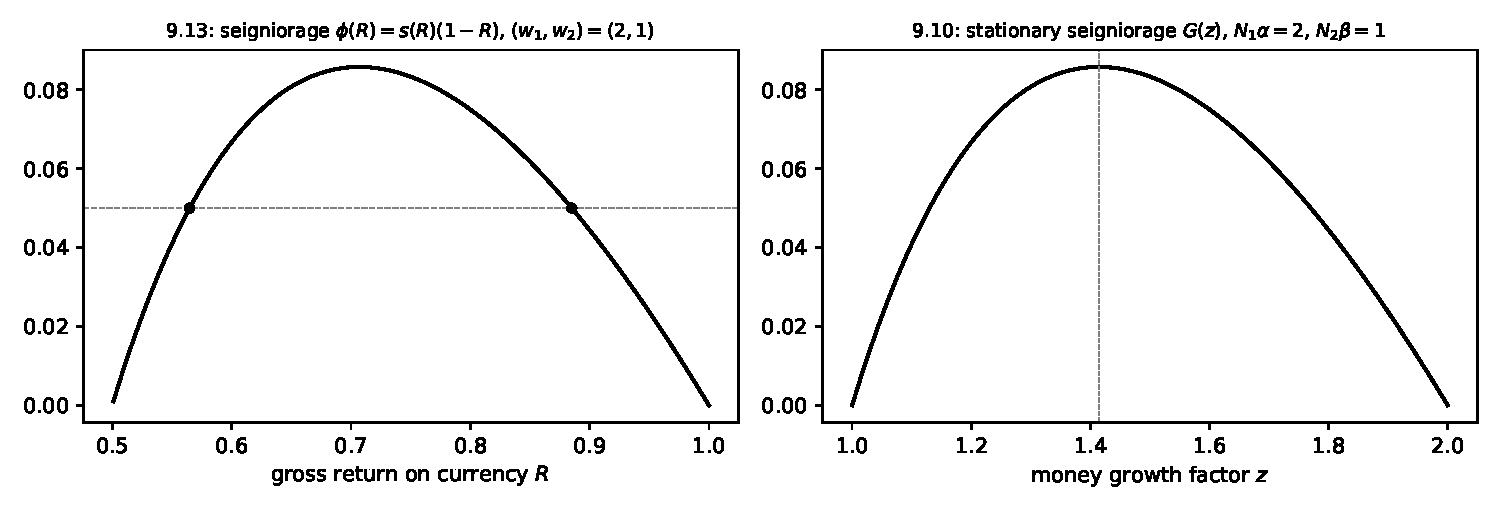
\includegraphics[width=\textwidth]{figures/ch9_laffer.pdf}\\
{\small Figure S9.2.  Left: stationary seigniorage $\phi(R)$ in Exercise 9.13 with $(w_1,w_2)=(2,1)$; $g=.05$ is raised at two returns.  Right: stationary seigniorage as a function of money growth in
Exercise 9.10 ($N_1\alpha=2$, $N_2\beta=1$); revenue peaks at $z^*=\sqrt2$, well before $z_{\max}=2$.}
\end{center}
\end{ex}

%% ===========================================================================
%% Chapter 11. Fiscal Policies in a Growth Model
%% ===========================================================================
\solchapter{11}{Fiscal Policies in a Growth Model}

\begin{center}
\begin{minipage}{0.86\textwidth}
\small
Solutions to all 20 exercises of Chapter 11 of Ljungqvist and Sargent, \emph{Recursive Macroeconomic Theory} (4th edition, 2018).
Numerical results and figures come from \texttt{code/ch11.py}, which replaces the book's Matlab and Dynare programs: it computes
perfect-foresight equilibria by Newton's method on the stacked Euler equations and checks them against the book's shooting algorithm and
its linear approximation.
\end{minipage}
\end{center}

\bigskip
\hrule
\bigskip

\emph{Equilibrium conditions.}  Throughout, $u(c)=c^{1-\gamma}/(1-\gamma)$ ($\log c$ if $\gamma=1$), $\beta=1/(1+\rho)$, and, unless said otherwise,
$f(k)=zk^\alpha$ and labor is supplied inelastically.  In a competitive equilibrium with time-0 trading the firm sets $\eta_t=f'(k_t)$ and
$w_t=f(k_t)-k_tf'(k_t)$ \bk{(11.5.7)}.  Bounded household budget sets require the no-arbitrage conditions
$q_t=q_{t+1}[(1-\tau_{k,t+1})(\eta_{t+1}-\delta)+1]$ \bk{(11.5.2)}.  The household's first-order condition is $\beta^tu'(c_t)=\mu q_t(1+\tau_{ct})$
\bk{(11.5.5a)}, and $\lim_Tq_Tk_{T+1}=0$.  Eliminating prices, an equilibrium allocation satisfies feasibility
$c_t+g_t+k_{t+1}=f(k_t)+(1-\delta)k_t$, the initial condition, the terminal condition \bk{(11.5.3)}, and
\[
  u'(c_t)=\beta u'(c_{t+1})\bar R_{t+1},\qquad
  \bar R_{t+1}=\frac{1+\tau_{ct}}{1+\tau_{c,t+1}}\bigl[(1-\tau_{k,t+1})(f'(k_{t+1})-\delta)+1\bigr].\tag{E}
\]
With constant policy the steady state solves $f'(\bar k)=\delta+\rho/(1-\tau_k)$ \bk{(11.6.7)}, and $\bar R=1+\rho$.  Lump-sum taxes appear nowhere
in these conditions.

\emph{Linear approximation.}  Let $x_t=k_t-\bar k$.  Around a steady state with constant taxes, feasibility gives $\hat c_t=Px_t-x_{t+1}$, where
$P=f'(\bar k)+1-\delta$ is the pre-tax gross return, and the log of (E) gives $\gamma(\hat c_{t+1}-\hat c_t)/\bar c=\beta(1-\tau_k)f''(\bar k)x_{t+1}$.  Hence
\[
  x_{t+2}-(1+P+A)x_{t+1}+Px_t=0,\qquad A\equiv-\beta\bar c(1-\tau_k)f''(\bar k)/\gamma>0 .
\]
The characteristic polynomial is $P>0$ at $\lambda=0$ and $-A<0$ at $\lambda=1$, so it has one root $\lambda_2\in(0,1)$ and one root $\lambda_1=P/\lambda_2>1$ (with
$\tau_k=0$, $P=1/\beta$ and $\lambda_1\lambda_2=1/\beta$).  $\lambda_2$ is the feedback coefficient of \bk{(11.10.8)} and $1/\lambda_1$ the rate at which
foreseen future policy is discounted.  Since $A\propto1/\gamma$, $\lambda_2$ rises from $0$ as $\gamma\to0$ to $1$ as $\gamma\to\infty$.

\emph{Computation.}  For a policy that is constant from some date on, \texttt{ch11.py} stacks (E) for $t=0,\dots,S-2$ ($S=300$) and solves for
$k_1,\dots,k_{S-1}$ by Newton's method (the Jacobian is tridiagonal), with $k_0$ given and the terminal condition $k_S-\bar k=\lambda_2(k_{S-1}-\bar k)$ of the
terminal steady state.  This is the book's two-point boundary value problem (section \bk{11.6.3}), solved in a way that stays accurate over long
horizons.  Checks: an unchanged policy starting from its steady state returns the constant path exactly; $S=600$ changes no digit; the book's shooting
algorithm reproduces $c_0$ to $5\times10^{-10}$, and the linear approximation \bk{(11.10.8)} is within $0.015$ of the nonlinear path (both in exercise 11.17).
Where an exercise leaves parameters open we use those of section \bk{11.9}: $\alpha=.33$, $\delta=.2$, $\beta=.95$ ($1+\rho=1.0526$), $\gamma=2$, $z=1$,
$g=.2$.  Then $\bar k=1.4900$, $f(\bar k)=1.1406$, $\bar c=0.6426$, and $\lambda_2=0.8524$.

%%---------------------------------------------------------------------------
\begin{ex}{11.1}{Tax reform: I}
\exnote{Equation (1) refers to a numbered display of the exercise in the book.}
\textbf{(a)}  A competitive equilibrium is a budget-feasible policy $\{g_t,\tau_{ct},\tau_{ht}\}$ (one that satisfies (1)), a feasible allocation
$\{c_t,k_{t+1}\}$, and a price system $\{q_t,\eta_t,w_t\}$ such that, given the prices and the policy, the allocation solves the household's problem
($k_0$ given) and $\{k_t,n_t=1\}$ solves the firm's problem.  As shown in the introduction, it is characterized by feasibility, the terminal condition and
(E) with $\tau_{kt}=0$: $u'(c_t)/(1+\tau_{ct})=\beta u'(c_{t+1})[f'(k_{t+1})+1-\delta]/(1+\tau_{c,t+1})$.

\textbf{(b)}  With $\tau_{ct}=0$, (E) is the planner's Euler equation.  In a steady state $c_{t+1}=c_t$, so $\bar k_0$ solves $f'(\bar k_0)=\rho+\delta$ (the
augmented golden rule), and $\bar c=f(\bar k_0)-\delta\bar k_0-g$.  The capital-labor ratio does not depend on $g$.

\textbf{(c)}  Let an allocation, prices and a policy $\{g_t,0,\tau_{ht}\}$ be an equilibrium, and let $\{\tilde\tau_{ht}\}$ be another sequence with
$\sum_tq_t\tilde\tau_{ht}=\sum_tq_t\tau_{ht}$.  Lump-sum taxes enter the household's budget only through $\sum_tq_t\tau_{ht}$, so its budget set and its
optimal choice are unchanged.  They do not enter the firm's problem or feasibility, and (1) still holds.  So the same allocation and prices are an
equilibrium under $\{\tilde\tau_{ht}\}$.  Equivalently, the equilibrium conditions (E), feasibility and the terminal condition do not involve $\tau_h$; only the
present value $\sum_tq_t\tau_{ht}=\sum_tq_tg_t$ matters, and (1) pins it down.  (This is Ricardian equivalence: government borrowing and lending absorb any
retiming.)

\textbf{(d)}  A constant $\tau_c$ cancels from (E), so the equilibrium conditions are those of part (b): the allocation is the planning allocation with $g$
deducted.  From $k_0=\bar k_0$ it is $k_t=\bar k_0$ and $c_t=\bar c$ for all $t$.  The new steady state is the old one, and there is no transition.  With
constant consumption $q_t=\beta^tq_0$, and (1) becomes $\tau_c\bar c\sum_t\beta^t=g\sum_t\beta^t$:
\[
  \tau_c=g/\bar c .
\]
With inelastic labor, a constant consumption tax taxes the household's initial wealth, since its budget reads
\[
  (1+\tau_c)\sum_tq_tc_t=(\eta_0+1-\delta)q_0k_0+\sum_tq_tw_t ;
\]
so it is equivalent to a lump-sum tax.  Pre-tax prices are unchanged.  With the chapter's parameters, $\bar k_0=1.4900$, $\bar c=0.6426$ and $\tau_c=0.3112$.

\textbf{(e)}  The tax is constant from $t=10$ on, so the steady state again has $f'(k)=\rho+\delta$: the same $\bar k_0$ and $\bar c$.  But (E) at $t=9$ reads
\[
  u'(c_9)=\beta u'(c_{10})\,\frac{f'(k_{10})+1-\delta}{1+\tau_c}.
\]
A foreseen increase of the consumption tax is a tax on saving between $t=9$ and $t=10$, at rate $\tau_c/(1+\tau_c)$ on the gross return; at all other
dates (E) is undistorted.  The transition is that of Figure \bk{11.9.4}.  Consumption jumps up at $t=0$, and households run down capital to consume before
consumption becomes expensive.  The falling capital stock raises $\bar R_{t+1}=f'(k_{t+1})+1-\delta$ above $1+\rho$, so consumption keeps rising until $t=9$.
At $t=10$, $\bar R_{10}$ collapses and consumption falls sharply.  Afterwards the economy climbs back to $\bar k_0$ along the undistorted saddle path, with
$\bar R_t>1+\rho$ and rising consumption.

The tax rate now solves a fixed point, because the path depends on it:
\[
  \tau_c\sum_{t\ge10}q_t(\tau_c)\,c_t(\tau_c)=g\sum_{t\ge0}q_t(\tau_c).
\]
We solve it by an outer root-finder on $\tau_c$ around the Newton solution for the path.  The result is $\tau_c=0.6239$, twice the rate of policy (d):
nothing is collected for ten years, so the government borrows and must service the debt forever, and the tax base after $t=10$ is smaller.  Capital falls
from $1.490$ to $1.127$ at $t=10$.  Consumption jumps from $0.6426$ to $0.6584$ at $t=0$, rises to $0.7024$ at $t=9$, drops to $0.5647$ at $t=10$
($\bar R_{10}=0.680$), and recovers.  Government debt, from $B_t=R_{t-1,t}B_{t-1}+g_t-T_t$ \bk{(11.4.2)} with $T_t=\tau_{ct}c_t$, reaches $B_9=2.80$ and
converges to $3.818$, where the primary surplus $\tau_c\bar c-g$ equals the interest $\rho B$ (a check on the computation).
\begin{center}
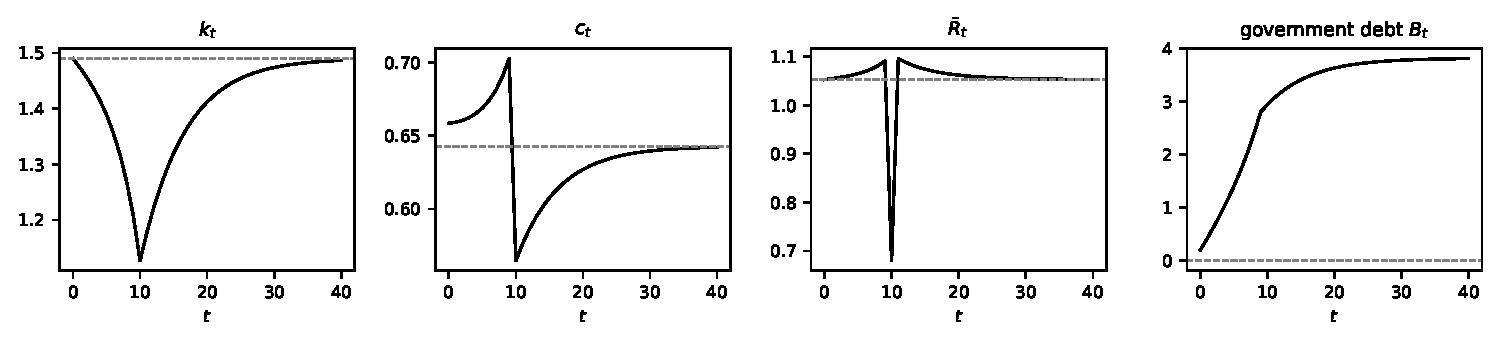
\includegraphics[width=\textwidth]{figures/ch11_01.pdf}\\
{\small Figure S11.1.  Policy (e): the consumption tax rises from $0$ to $0.624$ at $t=10$.  Dashed lines: the path under policy (d), which is the initial steady
state.}
\end{center}

\textbf{(f)}  Policy (d).  Its allocation satisfies the Euler equation, feasibility and the transversality condition of the planning problem
$\max\sum_t\beta^tu(c_t)$ subject to $c_t+g+k_{t+1}\le f(k_t)+(1-\delta)k_t$, $k_0=\bar k_0$.  That problem is strictly concave, so this is its unique solution.
The allocation under (e) is feasible but violates the planner's Euler equation at $t=9$, so it yields strictly lower utility.  Postponing the tax does not
ease the pain; it creates an intertemporal distortion: too much consumption before $t=10$, too little afterwards, and a capital stock that is run down and
rebuilt.  The welfare cost equals a permanent $0.435\%$ cut in consumption.
\end{ex}

%%---------------------------------------------------------------------------
\begin{ex}{11.2}{Tax reform: II}
\textbf{(a)}  As in exercise 11.1(a), with a budget-feasible policy $\{g_t,\tau_{ct},\tau_{kt}\}$.  The equilibrium is characterized by feasibility, the
terminal condition and (E) with both taxes.

\textbf{(b)}  In a steady state (E) gives $1=\beta[(1-\tau_k)(f'(\bar k_0)-\delta)+1]$, so
\[
  f'(\bar k_0)=\delta+\frac{\rho}{1-\tau_k},\qquad \bar c_0=f(\bar k_0)-\delta\bar k_0-g .
\]
The pre-tax net return on capital is $f'(\bar k_0)-\delta=\rho/(1-\tau_k)$; the after-tax return is $\rho$ ($\bar R=1+\rho$).  In a steady state $q_t\propto\beta^t$,
and the government budget reduces to period-by-period balance, which determines $\tau_k$:
\[
  g=\tau_k\bigl(f'(\bar k_0)-\delta\bigr)\bar k_0=\frac{\tau_k\rho}{1-\tau_k}\,\bar k_0(\tau_k).
\]
The right side is a Laffer curve.  It is zero at $\tau_k=0$ and, for $f=zk^\alpha$, tends to zero as $\tau_k\to1$, because then
$\bar k_0\propto(1-\tau_k)^{1/(1-\alpha)}$.  A $g$ below the peak has two solutions, and the equilibrium tax rate is the smaller one; the larger is on the wrong
side of the Laffer curve.
\rmk{With the chapter's calibration the peak revenue is $0.146$ (at $\tau_k=0.907$), so a capital tax cannot finance $g=.2$: its base, capital income net of
depreciation, is only $\rho\bar k_0/(1-\tau_k)$.  We use $g=.05$.  Then $\tau_k=0.4454$ (the other root is $0.9964$), $\bar k_0=1.1827$, $\bar c_0=0.7704$, and
the pre-tax net return is $0.0949$.}

\textbf{(c)}  A constant consumption tax cancels from (E), so the new equilibrium is the planning allocation from $\bar k_0$, with $g$ deducted.  Capital rises
monotonically to $\bar k$ with $f'(\bar k)=\rho+\delta$, which exceeds $\bar k_0$ because $f'$ is decreasing.  Steady-state consumption
$\bar c=f(\bar k)-\delta\bar k-g$ rises too: $f(k)-\delta k$ increases below the golden rule ($f'(k)>\delta$), and $\bar k_0<\bar k$ both lie below it.  The
pre-tax return on capital falls from $\rho/(1-\tau_k)$ to $\rho$.  The after-tax return is $1+\rho$ in both steady states; during the transition
$\bar R_{t+1}=f'(k_{t+1})+1-\delta$ exceeds $1+\rho$ and falls.  In our example $\bar k=1.4900$, $\bar c=0.7926$, and the consumption tax is
$\tau_c=\sum_tq_tg/\sum_tq_tc_t=0.0646$.  Consumption drops at $t=0$ to $0.7220$, below $\bar c_0$, because investment rises, and it stays below $\bar c_0$
for seven periods; $\bar R_1=1.0871$.

\textbf{(d)}  No.  The comparison ignores the transition: the larger capital stock of the new steady state must be accumulated, which requires lower
consumption first.  The right measure evaluates $\sum_t\beta^tu(c_t)$ along the equilibrium path from the common initial condition $\bar k_0$, against
$u(\bar c_0)/(1-\beta)$ for keeping the capital tax.  In our example, the steady-state comparison implies a gain equal to a permanent $2.89\%$ increase in
consumption, while the true gain is $0.60\%$.  The sign is right here, because the new allocation solves the planning problem from $\bar k_0$, for which
remaining at $\bar k_0$ is feasible.  In general, steady-state comparisons can even get the sign wrong: steady-state consumption is largest at the golden
rule (exercise 11.5), yet moving there from $\bar k$ lowers welfare.
\end{ex}

%%---------------------------------------------------------------------------
\begin{ex}{11.3}{Anticipated productivity shift}
\textbf{(a)}  Choose $\{c_t,x_t,k_{t+1}\}$ to maximize $\sum_t\beta^tu(c_t)$ subject to the two constraints, with $k_0$ given.  The Lagrangian is
\[
  L=\sum_t\beta^t\bigl\{u(c_t)+\mu_t[f(k_t)-c_t-x_t]+\lambda_t[(1-\delta)k_t+\psi_tx_t-k_{t+1}]\bigr\}.
\]
The first-order conditions are $u'(c_t)=\mu_t$, $\mu_t=\psi_t\lambda_t$ and $\lambda_t=\beta[\mu_{t+1}f'(k_{t+1})+(1-\delta)\lambda_{t+1}]$, plus
$\lim_t\beta^t\lambda_tk_{t+1}=0$.  So $\lambda_t=u'(c_t)/\psi_t$: installed capital is worth $1/\psi_t$ units of consumption, and
\[
  \frac{u'(c_t)}{\psi_t}=\beta u'(c_{t+1})\Bigl[f'(k_{t+1})+\frac{1-\delta}{\psi_{t+1}}\Bigr].\tag{1}
\]
With constant $\psi$ the steady state solves $f'(\bar k)=(\rho+\delta)/\psi$, with $\bar x=\delta\bar k/\psi$ and $\bar c=f(\bar k)-\delta\bar k/\psi$.  A permanent
increase in $\psi$ lowers $f'(\bar k)$, so $\bar k$ rises: $d\log\bar k/d\log\psi=1/\varepsilon$, where $\varepsilon=-\bar kf''(\bar k)/f'(\bar k)$.
Consumption rises: $d\bar c/d\psi=[f'(\bar k)-\delta/\psi]\,d\bar k/d\psi+\delta\bar k/\psi^2=(\rho/\psi)\,d\bar k/d\psi+\delta\bar k/\psi^2>0$.  Investment in
efficiency units, $\psi\bar x=\delta\bar k$, rises, and $d\log\bar x/d\log\psi=1/\varepsilon-1$, so investment in goods rises iff $\varepsilon<1$.  For
Cobb--Douglas $\varepsilon=1-\alpha$, so $\bar x\propto\psi^{\alpha/(1-\alpha)}$ rises.  With the chapter's parameters and no government: $\psi=1$ gives
$(\bar k,\bar c,\bar x)=(1.490,0.843,0.298)$, and $\psi=2$ gives $(4.192,1.186,0.419)$.

\textbf{(b)}  Because $\psi_t$ depends on calendar time, the state must record the date relative to the switch.  Let $s_t=\min\{t,4\}$, with
$s_{t+1}=\min\{s_t+1,4\}$, $\psi(s)=1$ for $s\le3$ and $\psi(4)=2$ (we take $\psi_0=1$; the exercise defines $\psi_t$ only for $t\ge1$).  The state is $(k_t,s_t)$,
the control $k_{t+1}$, and
\[
  V(k,s)=\max_{k'}\Bigl\{u\Bigl(f(k)-\frac{k'-(1-\delta)k}{\psi(s)}\Bigr)+\beta V\bigl(k',\min\{s+1,4\}\bigr)\Bigr\}.
\]
For $s=4$ this is the stationary Bellman equation of the economy with $\psi=2$ forever; $V(\cdot,3),\dots,V(\cdot,0)$ follow by four backward steps.  The
state evolves as $k_{t+1}=h_{s_t}(k_t)$ and $s_{t+1}=\min\{s_t+1,4\}$.

\textbf{(c)}  A price system is $\{q_t,\eta_t,w_t\}$: $q_t$ is the time-0 price of a time-$t$ good (consumption or investment), $\eta_t$ the rental rate of capital
and $w_t$ the wage, both in time-$t$ goods.  The household maximizes $\sum_t\beta^tu(c_t)$ subject to $\sum_tq_t(c_t+x_t)\le\sum_tq_t(\eta_tk_t+w_t)$ and
$k_{t+1}=(1-\delta)k_t+\psi_tx_t$, $k_0$ given.  Substituting $x_t=[k_{t+1}-(1-\delta)k_t]/\psi_t$, its first-order conditions are
\[
  \beta^tu'(c_t)=\mu q_t,\qquad \frac{q_t}{\psi_t}=q_{t+1}\Bigl[\eta_{t+1}+\frac{1-\delta}{\psi_{t+1}}\Bigr],
\]
together with $\lim_tq_tk_{t+1}/\psi_t=0$.  The second condition is a no-arbitrage condition: a unit of capital costs $q_t/\psi_t$ at $t$ and returns the
rental plus undepreciated capital worth $1/\psi_{t+1}$ goods at $t+1$.  The firm maximizes $\sum_tq_t[f(k_t)n_t-\eta_tk_tn_t-w_tn_t]$, so
$\eta_t=f'(k_t)$ and $w_t=f(k_t)-k_tf'(k_t)$.

\textbf{(d)}  Substituting the firm's conditions into the household's gives exactly (1).  Feasibility holds because
$c_t+x_t=\eta_tk_t+w_t=f(k_t)$, and the transversality conditions coincide.  So the equilibrium allocation is the planning allocation, and the planning
allocation with $q_t=\beta^tu'(c_t)/u'(c_0)$, $\eta_t=f'(k_t)$ and $w_t=f(k_t)-k_tf'(k_t)$ is an equilibrium.  The price $q_t$ is the (normalized) multiplier
$\beta^t\mu_t/\mu_0$ on the time-$t$ resource constraint; $\eta_t$ and $w_t$ are marginal products; and the price of installed capital, $1/\psi_t$ goods, is
the ratio $\lambda_t/\mu_t$ of the multipliers.

\textbf{(e)}  Yes, the jump has effects that precede it.  From $t=4$ on, a unit of goods buys two units of capital.  This makes the economy richer, so
consumption rises at $t=0$ already.  It also imposes a capital loss: capital carried from $t=3$ into $t=4$ is worth only $1/\psi_4=1/2$ good at $t=4$, so
the gross return between $t=3$ and $4$ collapses to $f'(k_4)+(1-\delta)/2$.  Anticipating this, the household postpones investment until it becomes cheap:
investment falls below its old steady-state level from $t=0$ on, and capital declines until $t=4$.  By (1), consumption must then fall between $t=3$ and $4$,
when the investment boom starts; afterwards the return is high and consumption rises toward the new steady state.  The computed path is:
\begin{center}
\begin{tabular}{lcccccccc}
\toprule
$t$ & 0 & 1 & 2 & 3 & 4 & 5 & 6 & $\infty$\\
\midrule
$k_t$ & $1.490$ & $1.432$ & $1.367$ & $1.292$ & $1.201$ & $1.592$ & $1.955$ & $4.192$\\
$c_t$ & $0.901$ & $0.904$ & $0.910$ & $0.921$ & $0.747$ & $0.825$ & $0.888$ & $1.186$\\
$x_t$ & $0.240$ & $0.222$ & $0.198$ & $0.167$ & $0.315$ & $0.341$ & $0.360$ & $0.419$\\
$R_{t,t+1}$ & $1.059$ & $1.068$ & $1.078$ & $0.692$ & $1.283$ & $1.221$ & $1.180$ & $1.053$\\
\bottomrule
\end{tabular}
\end{center}
Here $R_{t,t+1}=\psi_t[f'(k_{t+1})+(1-\delta)/\psi_{t+1}]$ is the gross real interest rate.  Consumption jumps from $0.843$ to $0.901$ at $t=0$ and investment
falls from $0.298$ to $0.240$.  Investment stays positive throughout (its minimum is $0.167$ at $t=3$), so requiring $x_t\ge0$ would change nothing
(Figure S11.2).
\begin{center}
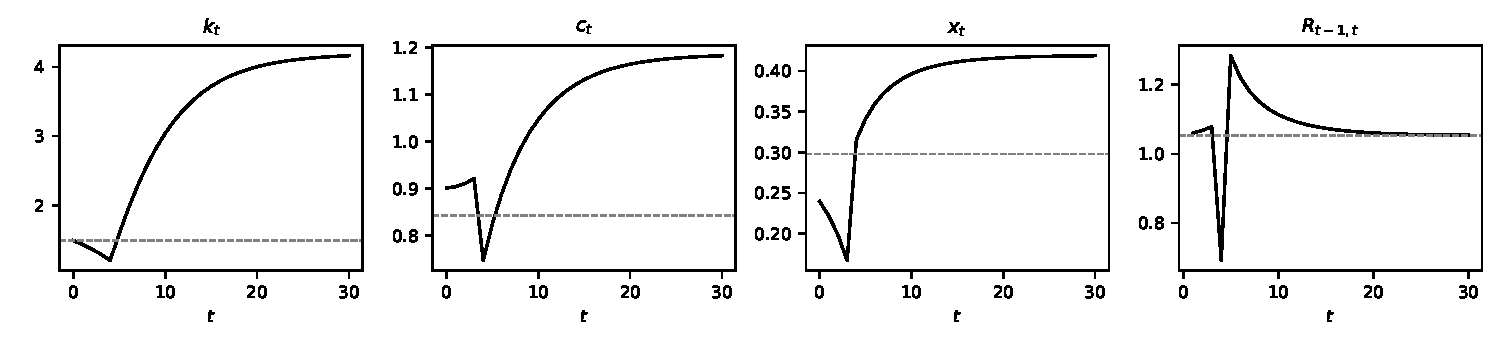
\includegraphics[width=\textwidth]{figures/ch11_03.pdf}\\
{\small Figure S11.2.  Response to the investment-technology shift at $t=4$, foreseen at $t=0$.  Dashed lines: the initial steady state.}
\end{center}
\end{ex}

%%---------------------------------------------------------------------------
\begin{ex}{11.4}{A capital levy}
\textbf{(a)}  The levy is a bill of $\varphi k_T$ time-$T$ goods.  (If it is a fraction of the value $(\eta_T+1-\delta)k_T$ instead, rescale $\varphi$.)  The
household maximizes $\sum_t\beta^tu(c_t)$ subject to
\[
  \sum_tq_t[c_t+k_{t+1}-(1-\delta)k_t]\le\sum_tq_t(\eta_tk_t+w_t)-q_T\varphi k_T ,
\]
$k_0$ given; the government's budget is $\sum_tq_tg_t=q_T\varphi k_T$.  A competitive equilibrium is a budget-feasible policy $(\{g_t\},\varphi,T)$, a
feasible allocation and prices such that household and firm optimize.  It is characterized by $\eta_t=f'(k_t)$, $w_t=f(k_t)-k_tf'(k_t)$, $\beta^tu'(c_t)=\mu q_t$,
the no-arbitrage conditions $q_{t-1}=q_t[\eta_t+1-\delta-\varphi\,\indic{t=T}]$ for $t\ge1$, feasibility and the terminal condition.  Hence
\[
  u'(c_t)=\beta u'(c_{t+1})\bigl[f'(k_{t+1})+1-\delta-\varphi\,\indic{t+1=T}\bigr].
\]
A levy at $T=0$ falls on the predetermined $k_0$, so it is a lump-sum tax.  A levy at $T\ge1$ taxes the gross return on capital carried from $T-1$ into $T$.

\textbf{(b)}  With $g\equiv0$ and no taxes, $f'(k_0)=\rho+\delta$, so $k_0=[\alpha A/(\rho+\delta)]^{1/(1-\alpha)}$.

\textbf{(c)}  The levy is lump sum, so the allocation is the planning allocation with $g$ deducted, and the steady state is again $f'(k)=\rho+\delta$: the new
steady-state capital stock is $k_0$.  Since the economy starts there, $k_t=k_0$, $c_t=f(k_0)-\delta k_0-g$ (lower by exactly $g$), and
$R_{t,t+1}=f'(k_0)+1-\delta=1+\rho$ for all $t$.  Only consumption differs from the $g\equiv0$ equilibrium.  To compute $\varphi$: (i) compute the equilibrium
allocation, which does not depend on $\varphi$; (ii) compute $q_t=\beta^tu'(c_t)/u'(c_0)$; (iii) set $\varphi=\sum_tq_tg_t/(q_0k_0)$.  Here $q_t=\beta^t$, so
\[
  \varphi=\frac{g}{(1-\beta)k_0}=\frac{(1+\rho)g}{\rho k_0}.
\]
It exceeds one when $g>(1-\beta)k_0$, and then the household pays part of the levy out of the present value of its wages.  Any
$g<f(k_0)-\delta k_0$ can be financed.  With $A=1$ and the chapter's other parameters, $k_0=1.490$; for $g=.02$, $\varphi=0.268$ and
consumption falls from $0.843$ to $0.823$.

\textbf{(d)}  After $t=10$ there are no taxes, so the steady state is again $k_0$.  But the levy now distorts the decision to carry capital into $t=10$:
\[
  u'(c_9)=\beta u'(c_{10})\,\bigl[f'(k_{10})+1-\delta-\varphi\bigr].
\]
\emph{Algorithm.}  For a trial $\varphi$, compute the equilibrium path from $k_0$ to the steady state, with this distorted Euler equation at $t=9$, by shooting
or Newton's method.  Compute $q_t$ and the budget gap $\Gamma(\varphi)=q_{10}\varphi k_{10}-\sum_tq_tg$, and solve $\Gamma(\varphi)=0$ by bisection or the secant
method, taking the smallest root.

\emph{A pitfall: the Laffer curve.}  The household can shrink the tax base $k_{10}$, so the revenue of a foreseen levy is bounded.  For each $\varphi$ we compute
(by continuation in $\varphi$) the $g$ that the levy finances.  It rises to a maximum of $g=0.0354$ at $\varphi=1.58$, where $k_{10}=0.216$ and the gross return
from $t=9$ to $10$ net of the levy is $0.14$, and then falls slowly.  So a surprise levy at $T=0$ can finance any feasible $g$ (up to $0.843$), while a levy
foreseen for $T=10$ can finance at most about $3\%$ of output.  We take $g=.02$.

\emph{Paths} (Figure S11.3).  The levy rate is $\varphi=0.494$, versus $0.268$ at $T=0$.  Anticipating the levy, the household consumes more and invests less
before $t=10$: capital falls from $1.490$ to $1.012$ at $t=10$.  Consumption starts at $0.840$ (above the $0.823$ of part (c), slightly below the $0.843$ of the
$g\equiv0$ equilibrium) and rises to $0.911$ at $t=9$, because the interest rate $R_{t,t+1}=f'(k_{t+1})+1-\delta$ exceeds $1+\rho$ as capital falls.  Between
$t=9$ and $10$ the return net of the levy is $0.633$, which forces consumption down to $0.707$ at $t=10$.  Then capital is rebuilt ($R_{10,11}=1.112$) and
consumption rises to $0.823$, the level of part (c).  The long run is the same as in (c); the transition is distorted, at a welfare cost equal to a permanent
$0.53\%$ of consumption.
\begin{center}
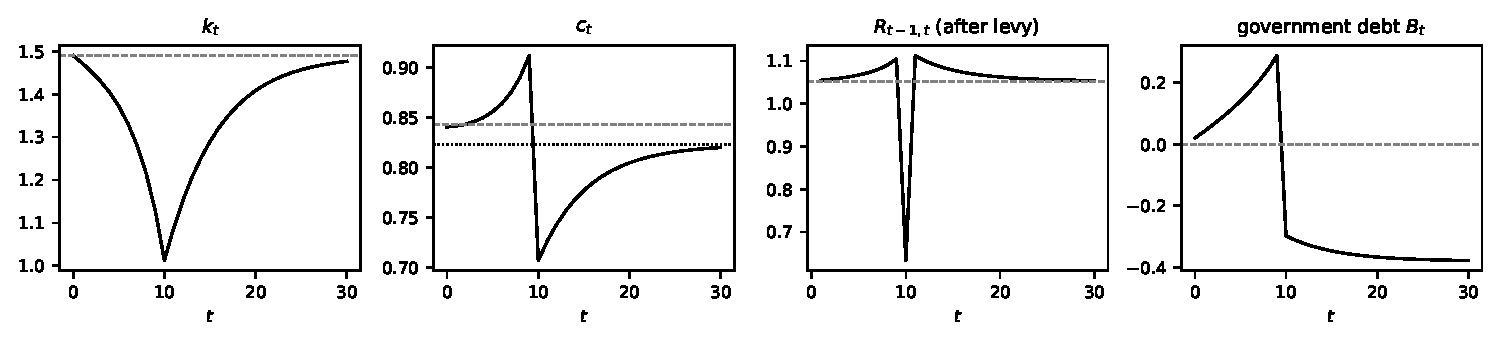
\includegraphics[width=\textwidth]{figures/ch11_04.pdf}\\
{\small Figure S11.3.  Levy at $T=10$ foreseen at $t=0$ ($g=.02$).  Dashed lines: the $g\equiv0$ steady state; dotted line: consumption with the levy at $T=0$.}
\end{center}

\textbf{(e)}  Without uncertainty, one-period Arrow securities are one-period bonds.  At each $t$ the household chooses $c_t$, $k_{t+1}$ and holdings $b_{t+1}$
of bonds that pay one good at $t+1$ and cost $1/R_{t,t+1}$, subject to
\[
  c_t+k_{t+1}+b_{t+1}/R_{t,t+1}\le(\eta_t+1-\delta)k_t+w_t+b_t-\varphi k_t\indic{t=T},\qquad b_0=0,
\]
and a natural borrowing limit.  The government satisfies $g_t+b^g_t=b^g_{t+1}/R_{t,t+1}+\varphi k_t\indic{t=T}$ with $b^g_0=0$, where $b^g_t$ is its debt
maturing at $t$.  An equilibrium is a policy, an allocation, bond holdings and prices $\{R_{t,t+1},\eta_t,w_t\}$ such that household and firm optimize and
the goods and bond markets clear ($b_t=b^g_t$).  To compute it, note that the allocation and $R_{t,t+1}=q_t/q_{t+1}$ are those of the time-0 equilibrium,
because one-period bonds complete the markets here; the debt follows from the government's constraint.  In the book's units, the value of debt issued at
$t$ satisfies $B_t=R_{t-1,t}B_{t-1}+g_t-T_t$ \bk{(11.4.2)}, where $T_t$ is the levy.

Under (d) the government borrows from the household to pay for $g$ until $t=9$: $B_0=0.020$ and $B_9=0.288$.  By no arbitrage, bonds earn the same return
as capital from $t=9$ to $10$, $R_{9,10}=0.633$, so bondholders share in the levy.  At $t=10$ the levy ($0.500$) pays off the debt, and the government
becomes a creditor: $B_{10}=-0.298$.  Its claims converge to $-g/\rho=-0.380$, whose interest pays for $g$ forever.  The household mirrors this: it holds
government bonds before $t=10$, and afterwards it is permanently in debt to the government, paying interest of about $g$ per period.
\end{ex}

%%---------------------------------------------------------------------------
\begin{ex}{11.5}{A permanent increase in government purchases}
\textbf{(a)}  $f'(k)=\rho+\delta$, so $k=[\alpha z/(\rho+\delta)]^{1/(1-\alpha)}$.

\textbf{(b)}  The golden rule solves $f'(\tilde k)=\delta$, so $\tilde k=(\alpha z/\delta)^{1/(1-\alpha)}>k$, because $\rho>0$ and $f'$ is decreasing.  Since $\tilde k$
maximizes $f(k)-\delta k$ and $k\neq\tilde k$, $\tilde c>c$.  Raising capital from $k$ to $\tilde k$ would increase steady-state consumption, but the extra capital
must be accumulated by consuming less first, and the household discounts the later gains.  At $k$, the marginal gain in steady-state consumption,
$f'(k)-\delta=\rho$, exactly compensates for impatience (the modified golden rule).  With the chapter's parameters, $k=1.490$ and $c=0.8426$, while
$\tilde k=2.112$ and $\tilde c=0.8574$.

\textbf{(c)}  $g=c/2$ is feasible.  We claim $k_t=k$, $c_t=c-g=c/2$ and $\bar R_{t+1}=1+\rho$ for all $t$.  This path satisfies feasibility
($c/2+g+k=f(k)+(1-\delta)k$), the Euler equation ($c_t$ constant and $f'(k)+1-\delta=1/\beta$), the initial condition and the transversality condition
$\lim_t\beta^tk/c_t=0$.  With lump-sum taxes the equilibrium is the planning allocation with $g$ deducted (section \bk{11.8}); that problem is strictly concave,
so these conditions are sufficient and the path is the unique equilibrium.  (\texttt{ch11.py} confirms that the Newton solver returns this constant path.)
The reason: $g$ does not enter the steady-state condition $f'(k)=\rho+\delta$, and a permanent, unforeseen increase in $g$ is a permanent loss of resources for
private use.  A consumption-smoothing household absorbs it entirely by consuming less, at once and forever, as in the permanent income theory.  There is
nothing to gain from changing the capital stock, so the interest rate does not move.
\end{ex}

%%---------------------------------------------------------------------------
\begin{ex}{11.6}{Trade and growth}
\textbf{(a)}  $f'(\bar k)=\rho+\delta$, so $\bar k=[\alpha z/(\rho+\delta)]^{1/(1-\alpha)}$.

\textbf{(b)}  The value function $V$ is strictly concave, and the optimal policy $k'=h(k)$ is strictly increasing, because the objective
$u(f(k)+(1-\delta)k-k')+\beta V(k')$ has strictly increasing differences in $(k,k')$.  Consumption $c(k)=f(k)+(1-\delta)k-h(k)$ is also increasing: the
first-order condition $u'(c(k))=\beta V'(h(k))$ has a right side that falls with $k$.  The positive fixed points of $h$ satisfy the steady-state Euler equation,
so $\bar k$ is the only one.  If $h(k)\le k$ for some $k<\bar k$, then (as $h$ is increasing and continuous) $k_t$ would decrease monotonically to a fixed point
below $\bar k$, which would have to be $0$.  That is impossible: as $k_t\to0$, $f'(k_{t+1})\to\infty$, and the Euler equation would make consumption grow without
bound while resources shrink to zero.  So $h(k)>k$ on $(0,\bar k)$.  Therefore, from $k_0<\bar k$, $k_t$ rises monotonically to $\bar k$, $c_t$ rises
monotonically to $\bar c=f(\bar k)-\delta\bar k$, and $\bar R_{t+1}=1-\delta+f'(k_{t+1})$ falls monotonically.  The Euler equation
$(c_{t+1}/c_t)^\gamma=\beta\bar R_{t+1}>1$ confirms that consumption grows while the return exceeds $1+\rho$.  With $k_0=.5\bar k$ and $\gamma=2$ (our choice),
$c$ rises from $0.648$ to $0.843$ and $\bar R_1=1.166$.

\textbf{(c)}  $\bar R=1+\rho=1/\beta$.

\textbf{(d)}  Above, since $f'$ is decreasing.

\textbf{Part II.}  Attach multipliers $\beta^t\lambda_t$ to the budget constraints for $t\ge0$, and substitute $k_0=\bar k_0+B_{-1}$.  The first-order conditions are
\[
  u'(c_t)=\lambda_t,\qquad \lambda_t=R\beta\lambda_{t+1}=\lambda_{t+1}\ (B_t),\qquad \lambda_t=\beta\lambda_{t+1}[f'(k_{t+1})+1-\delta]\ (k_{t+1}),
\]
and $f'(k_0)+1-\delta=R$ for $B_{-1}$.  Hence consumption is constant, and $f'(k_t)=\rho+\delta$ for all $t\ge0$: the planner borrows $B_{-1}=\bar k-\bar k_0$
and jumps to $k_t=\bar k$ at once.  The present-value budget (with $\lim_tR^{-t}B_t=0$) is $c/(1-\beta)=[f(\bar k)-\delta\bar k]/(1-\beta)-R(\bar k-\bar k_0)$,
so
\[
  c=f(\bar k)-\delta\bar k-\rho(\bar k-\bar k_0)=\bar w+\rho\bar k_0,\qquad \bar w\equiv f(\bar k)-\bar kf'(\bar k).
\]
The debt is rolled over forever, $B_t=\bar k-\bar k_0$, with interest $\rho B_t$.  The open economy reaches the steady-state capital stock at once, and its
consumption is constant: higher than the closed economy's consumption early on, but permanently below the closed economy's eventual
$\bar c=\bar w+\rho\bar k$, the difference being interest on the foreign debt.

Welfare is higher in the open economy.  Any closed-economy plan is feasible in the open economy (set $B_t=0$), and the closed-economy path is not optimal
there, because its consumption is not constant.  With $\bar k_0=.5\bar k$: $B_{-1}=0.745$ and $c=0.8034$.  The closed economy's path is worth as much as a
constant consumption of $0.7924$, so opening up is worth $1.39\%$ of consumption every period (Figure S11.4).  Comparing steady-state consumption ($0.803<0.843$)
would wrongly suggest that opening hurts (compare section \bk{11.13.5.1}).
\begin{center}
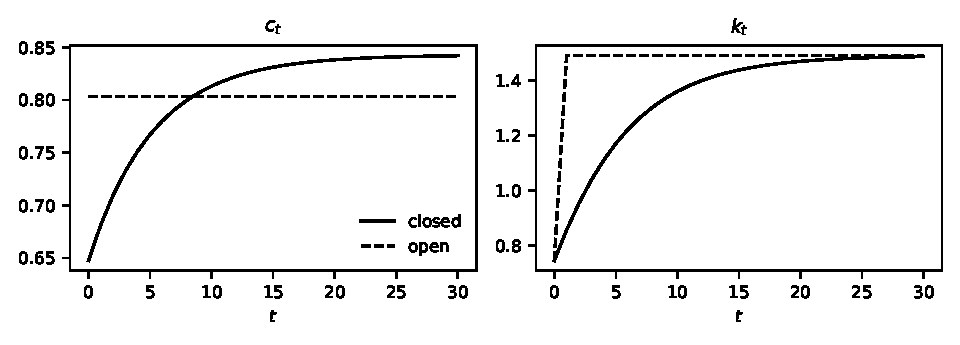
\includegraphics[width=0.66\textwidth]{figures/ch11_06.pdf}\\
{\small Figure S11.4.  Closed and open economy from $\bar k_0=.5\bar k$.}
\end{center}
\end{ex}

%%---------------------------------------------------------------------------
\begin{ex}{11.7}{A capital tax, unforeseen and foreseen}
\textbf{(a)}  $f'(\bar k)=\rho+\delta$, $\bar k=[\alpha z/(\rho+\delta)]^{1/(1-\alpha)}$, $\bar c=f(\bar k)-\delta\bar k-\bar g$ and $\bar R=1+\rho$.  With the chapter's
parameters: $\bar k=1.490$, $\bar c=0.6426$ and $\bar R=1.0526$.

\textbf{(b)}  The new steady state has $f'(\bar k')=\delta+\rho/(1-\tau_k)>\rho+\delta$, so $\bar k'<\bar k$; $\bar c'=f(\bar k')-\delta\bar k'-\bar g<\bar c$ (both lie
below the golden rule); and the after-tax return is again $\bar R=1+\rho$.  The change is unforeseen, so $k_0=\bar k$ is inherited, and the economy moves along
the new saddle path.  Since capital must fall ($k_1<k_0=\bar k$), consumption jumps up at $t=0$: $c_0=f(\bar k)+(1-\delta)\bar k-\bar g-k_1>\bar c$.  After that,
$k$ falls monotonically to $\bar k'$.  The return $\bar R_{t+1}=1+(1-\tau_k)(f'(k_{t+1})-\delta)$ drops below $1+\rho$ at $t=1$ and then rises back to $1+\rho$ as
capital falls.  Since $\bar R<1+\rho$, consumption declines monotonically to $\bar c'<\bar c$.  To a linear approximation $k_{t+1}-\bar k'=\lambda_2(k_t-\bar k')$,
and \texttt{ch11.py} confirms that all three paths are monotone.  With $\tau_k=.2$ (our choice) and $\gamma=2$: $\bar k'=1.381$, $\bar c'=0.6362$,
$c_0=0.6575$ and $\bar R_1=1.0435$ (Figure S11.5, top row).

\textbf{(c)}  Steady states do not depend on $\gamma$; the speed of adjustment does.  Near the new steady state,
$c_t-\bar c'\approx P(k_t-\bar k')-(k_{t+1}-\bar k')=(P-\lambda_2)(k_t-\bar k')$, with $P=f'(\bar k')+1-\delta$.  So the initial jump is
$c_0-\bar c'\approx(P-\lambda_2)(\bar k-\bar k')$, which is smaller the larger is $\lambda_2$, i.e.\ the larger is $\gamma$.  A household with low $\gamma$ is willing
to let consumption vary: it eats the excess capital quickly, with a big consumption spike, fast convergence and a quick return of $\bar R$ to $1+\rho$.  A
household with high $\gamma$ spreads the adjustment over many periods.  With $\gamma=.2$, $\lambda_2=0.599$, the jump is $+0.044$, and by $t=10$ capital has
essentially converged ($1.382$).  With $\gamma=2$, $\lambda_2=0.865$, the jump is $+0.015$, and $k_{10}=1.406$.  The formula
$(P-\lambda_2)(\bar k-\bar k')$ gives $0.051$ and $0.022$, against exact values $0.051$ and $0.021$.

\textbf{(d)}  i) As in (b): $\bar k'=1.381$, $\bar c'=0.636$, $\bar R=1+\rho$.

ii) Capital carried into periods $t\ge10$ will be taxed, so households begin to reduce their capital at once.  Before $t=10$ capital income is still untaxed,
so the falling capital stock raises $\bar R_{t+1}=1-\delta+f'(k_{t+1})$ above $1+\rho$, and by (E) consumption must rise.  Thus consumption jumps up slightly at
$t=0$ and keeps rising until $t=9$ ($\gamma=2$: from $0.6426$ to $0.6449$, then to $0.6502$; $\bar R_9=1.0571$).  At $t=10$ the tax cuts the after-tax
return to $\bar R_{10}=1.0466<1+\rho$, and consumption starts to decline toward $\bar c'$.  After $t=10$ only transient dynamics remain: capital keeps falling
to $\bar k'$ and $\bar R$ rises back to $1+\rho$ (Figure S11.5, bottom row, as in the book's Figure \bk{11.9.5}).

iii) Two decay rates govern the path: the feedback coefficient $\lambda_2$ after $t=10$, and the discount factor $1/\lambda_1=\lambda_2/P$ applied to future
policy before $t=10$ \bk{(11.10.8)}.  With $\gamma=2$, $\lambda_2=0.865$ and $1/\lambda_1=0.812$: anticipation effects reach far back, consumption responds at
$t=0$, capital starts falling at once, and convergence after $t=10$ is slow (the computed ratios $(k_{t+1}-\bar k')/(k_t-\bar k')$ approach $0.865$).  With
$\gamma=.2$, $\lambda_2=0.599$ and $1/\lambda_1=0.562$: almost nothing happens until a few periods before $t=10$ ($c_0=0.6428$), then there is a sharp consumption
boom that peaks at $0.670$ at $t=9$, and convergence after $t=10$ is fast.  Because $\lambda_1\lambda_2=P$, a sluggish feedback response goes together with a
long anticipation horizon: this is the logic of \bk{(11.10.16)}.
\rmk{Formula \bk{(11.10.16)} is misprinted.  As printed it gives $\lambda_2=3.53$ at $\gamma=2$, and $\lambda_2\to\infty$ as $\gamma\to\infty$, which is impossible
for a stable root.  Solving the linearization above with $\tau_k=0$, i.e.\ $\lambda^2-(1+R+a/\gamma)\lambda+R=0$ with $R=1/\beta$ and
$a=-\beta\bar cf''(\bar k)$, gives
\[
  \lambda_2=\frac{\gamma}{a_1\gamma+a_2+(a_3\gamma+a_4\gamma^2+a_5)^{1/2}},
\]
with exactly the book's constants: $a_1=\frac{1+R}{2R}=.975$, $a_2=\frac a{2R}=.0329$, $a_3=\frac{2(1+R)a}{4R^2}=.0642$,
$a_4=\frac{(R-1)^2}{4R^2}=.000625$ and $a_5=\frac{a^2}{4R^2}=.0011$.  With these rounded constants it matches the exact root to four decimals (e.g.\ $0.8524$ at
$\gamma=2$, $0.5779$ at $\gamma=.2$) and reproduces Figure \bk{11.10.1}.}
\begin{center}
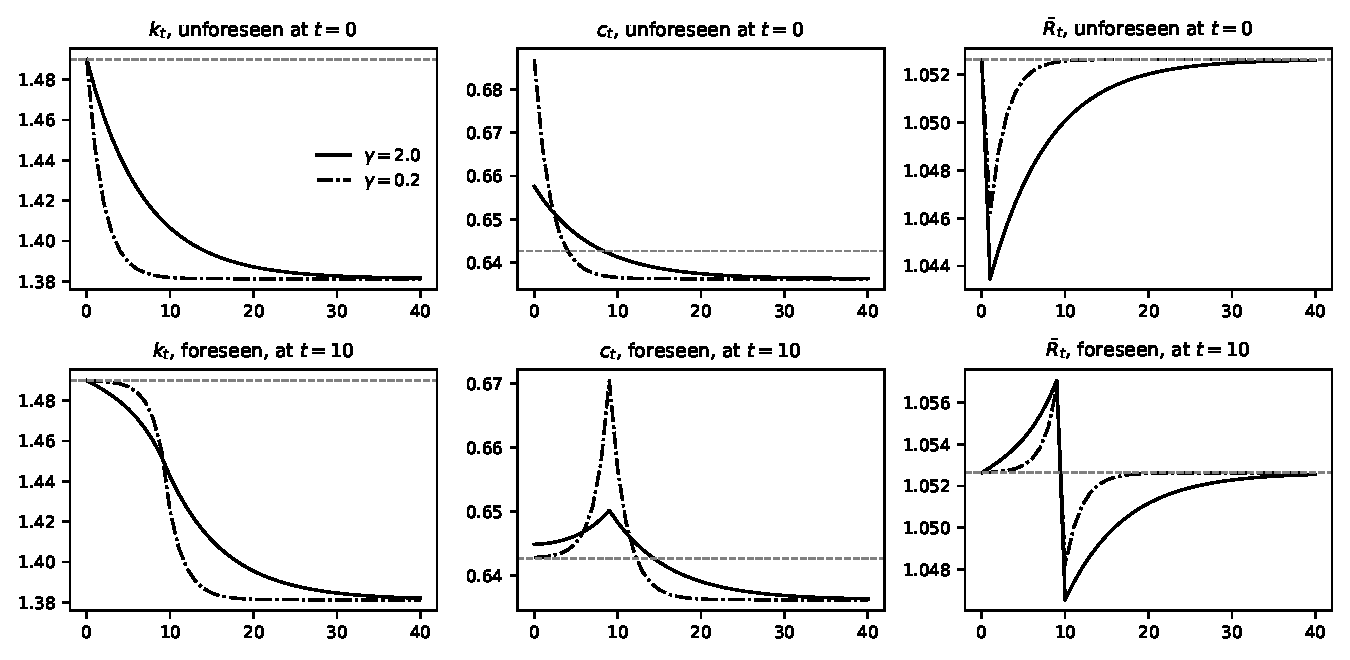
\includegraphics[width=\textwidth]{figures/ch11_07.pdf}\\
{\small Figure S11.5.  Capital tax $\tau_k=.2$, unforeseen at $t=0$ (top) or foreseen for $t=10$ (bottom); solid $\gamma=2$, dash-dotted $\gamma=.2$.  Dashed
lines: the initial steady state.}
\end{center}
\end{ex}

%%---------------------------------------------------------------------------
\begin{ex}{11.8}{Trade and growth, version II}
\rmk{The technology is printed as ``$c_t+k_t+1=f(k_t)+(1-\delta)k_t$'' (read $k_{t+1}$), and the ``where'' after it is followed by nothing; we take $u$ and $f$
from exercise 11.6.  Also, if $\bar k_0$ is sold at $t=-1$ for bonds that pay the gross rate $R$, then $A_0=R\bar k_0$; that is what ``consume the interest
payments'' means.  The printed $A_0=\bar k_0$ omits one period's interest.  We use $A_0=R\bar k_0$; with $A_0=\bar k_0$, replace $\rho\bar k_0$ below by
$(1-\beta)\bar k_0=\rho\bar k_0/R$.}

\textbf{(a)--(d)}  These mirror exercise 11.6.  $\bar k=[\alpha z/(\rho+\delta)]^{1/(1-\alpha)}$.  From $\bar k_0>\bar k$, the increasing policy $h$ satisfies $h(k)<k$ on
$(\bar k,\infty)$, so $k_t$ falls monotonically to $\bar k$, $c_t$ falls monotonically to $\bar c$, and $\bar R_{t+1}=1-\delta+f'(k_{t+1})$ rises monotonically to
$1+\rho$.  So the steady-state return is $\bar R=1+\rho$, and $\bar R_{t+1}<1+\rho$ while $k_{t+1}>\bar k$.  With $\bar k_0=2\bar k$ and $\gamma=2$: $c_0=1.117$,
$k_1=2.701$, $\bar R_1=0.970$, and $c$ falls to $0.843$.

\textbf{(e)}  With multipliers $\beta^t\ell_t$ on the budget constraints: $u'(c_t)=\ell_t$, and the condition for $A_{t+1}$,
$-\beta^t\ell_t\beta+\beta^{t+1}\ell_{t+1}=0$, gives $\ell_t=\ell_{t+1}$.  So consumption is constant.  The budget in
present value (no Ponzi games) is $\sum_t\beta^tc_t=A_0$, so $c_t=(1-\beta)A_0=\rho\bar k_0$ and $A_t=A_0$ for all $t$: the planner consumes the interest on its
wealth.

\textbf{(f)}  Under ``sell all'', capital is zero, consumption is constant at $\rho\bar k_0$, and the return is $1+\rho$.  In the closed economy, capital and
consumption fall toward $\bar k$ and $\bar c$, and the return rises toward $1+\rho$ from below.  The ranking depends on $\bar k_0$.  The closed economy can keep
capital at $\bar k_0$ and consume $f(\bar k_0)-\delta\bar k_0$ forever, and its optimal plan does strictly better than that.  So it is strictly preferred whenever
$f(\bar k_0)-\delta\bar k_0\ge\rho\bar k_0$, i.e.\ $f(\bar k_0)/\bar k_0\ge\rho+\delta=f'(\bar k)$; for Cobb--Douglas, iff $\bar k_0\le\alpha^{-1/(1-\alpha)}\bar k=5.23\bar k$.
For very large $\bar k_0$ the ranking reverses.  In a closed economy excess capital can only be eaten slowly, and meanwhile it earns
$1-\delta+f'(k)$, far less than the world rate $1+\rho$.  In the numerical example, ``sell all'' becomes better once $\bar k_0>14.6\bar k$.  Both plans are dominated by
the plan of part (g):
\begin{center}
\begin{tabular}{lcccccc}
\toprule
$\bar k_0/\bar k$ & $1.5$ & $2$ & $5$ & $10$ & $20$ & $40$\\
\midrule
closed economy & $-0.66\%$ & $-2.08\%$ & $-13.7\%$ & $-29.7\%$ & $-48.7\%$ & $-65.9\%$\\
sell all & $-86.7\%$ & $-83.0\%$ & $-66.1\%$ & $-49.4\%$ & $-32.8\%$ & $-19.6\%$\\
\bottomrule
\end{tabular}
\end{center}
The entries are welfare as a permanent percentage change of the consumption of plan (g) ($\gamma=2$).

\textbf{(g)}  i) This is exercise 11.6, Part II, with lending instead of borrowing ($B_{-1}<0$).  The planner sells $\bar k_0-\bar k$ at $t=-1$, keeps $k_t=\bar k$ for
all $t\ge0$ (where $f'(\bar k)+1-\delta=R$), holds foreign assets $\bar k_0-\bar k$ forever, and consumes
\[
  c=f(\bar k)-\delta\bar k+\rho(\bar k_0-\bar k)=\bar w+\rho\bar k_0,\qquad \bar w=f(\bar k)-\bar kf'(\bar k).
\]
ii) Plan (g) beats ``sell all'' by exactly the wage $\bar w=0.764$ per period: shutting down the technology wastes the country's labor endowment.  At the margin,
starting from zero capital, a unit of capital installed at $t-1$ returns $f'(k)+1-\delta$, which is infinite at $k=0$, while it costs $R$ in forgone bond income.
So it pays to install capital until $f'(k)=\rho+\delta$.  (The hint compares $z\epsilon^\alpha$ with $\rho\epsilon$ and ignores depreciation; including it, the
comparison is $z\epsilon^\alpha$ with $(\rho+\delta)\epsilon$, and the conclusion is the same.)
\end{ex}

%%---------------------------------------------------------------------------
\begin{ex}{11.9}{Linear utility with a finite horizon}
Let $W=\sum_{t=0}^TR^{-t}y_t>0$ and $d_t=R^{-t}c_t\ge0$, the present value of consumption at $t$.  The problem becomes
\[
  \max_{d\ge0}\ \sum_{t=0}^T(\beta R)^td_t\quad\text{subject to}\quad\sum_{t=0}^Td_t=W,
\]
a linear program over a simplex.  Its maximum puts all weight on the largest coefficient $(\beta R)^t$.

\textbf{(a)}  $\beta R<1$: the largest coefficient is at $t=0$.  So $c_0=W$ and $c_t=0$ for $t\ge1$: the consumer borrows against all future income and
consumes everything at once, because impatience beats the interest rate.

\textbf{(b)}  $\beta R>1$: the largest is at $t=T$.  So $c_T=R^TW=\sum_tR^{T-t}y_t$ and $c_t=0$ for $t<T$: the consumer saves everything and consumes at the end.

\textbf{(c)}  $\beta R=1$: all coefficients equal one.  Every nonnegative path with $\sum_tR^{-t}c_t=W$ is optimal, for instance $c_t=y_t$ or the constant path
$c_t=W(1-\beta)/(1-\beta^{T+1})$.  With linear utility there is no motive to smooth consumption, and only the comparison of $\beta$ with $R^{-1}$ shapes the path.
\end{ex}

%%---------------------------------------------------------------------------
\begin{ex}{11.10}{Term structure of interest rates}
\rmk{In the book's definition of $\bar R_{t+1}$, ``$f'(k_{t+1}-\delta)$'' should read $f'(k_{t+1})-\delta$, as in \bk{(11.6.8e)}.}

\textbf{(a)}  Consumption is constant at $\bar c$, so $q^0_t=\beta^tu'(c_t)/u'(c_0)=\beta^t$ (normalizing $q^0_0=1$).

\textbf{(b), (c)}  $r_{t-1,t}=\log(q^0_{t-1}/q^0_t)=-\log\beta=\log(1+\rho)=0.0513$ for every $t$, and hence $r_{0,t}=0.0513$ too: the yield curve is flat (the
dashed lines in Figure S11.6).

\textbf{(d)}  The equilibrium is that of exercise 11.7(b): consumption jumps up and then declines to $\bar c'$.  From $q^0_t=\beta^tu'(c_t)/u'(c_0)$,
\[
  r_{t-1,t}=-\log\beta+\gamma\log(c_t/c_{t-1})=\log\bar R_t,\qquad \bar R_t=1+(1-\tau_k)(f'(k_t)-\delta),
\]
where the second equality is (E).  i) Consumption declines at a decreasing rate, so the short rates are below $\log(1+\rho)$ and rising.  In economic terms,
the tax cuts the after-tax return at once ($\bar R_1=1.0435$), and as capital is run down the pre-tax marginal product rises, so the after-tax return
gradually returns to $1+\rho$.  With $\tau_k=.2$ and $\gamma=2$, $r_{0,1}=0.0426$ rising to $r_{9,10}=0.0489$.  ii) Yields average the short rates, so they
too lie below $\log(1+\rho)$ and rise: the yield curve slopes upward, from $r_{0,1}=0.0426$ to $r_{0,10}=0.0463$ (Figure S11.6).  (\texttt{ch11.py} checks that the
rates computed from $q^0_t$, from $\log\bar R_t$ and from the consumption path agree to $10^{-14}$.)
\begin{center}
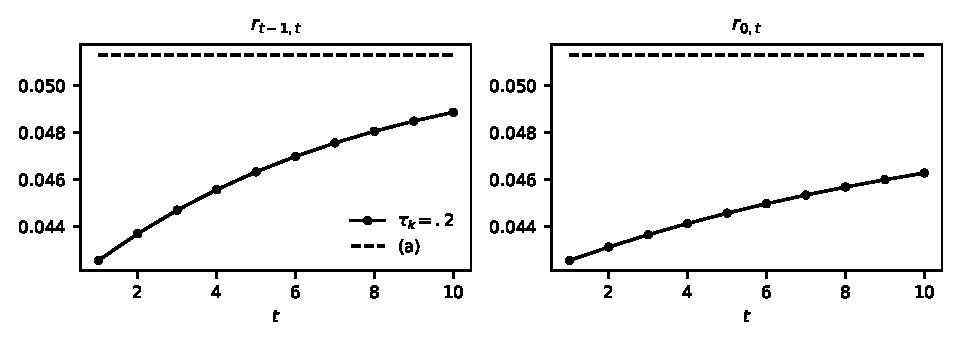
\includegraphics[width=0.66\textwidth]{figures/ch11_10.pdf}\\
{\small Figure S11.6.  Short rates and yields after an unforeseen permanent $\tau_k=.2$ at $t=0$; dashed: the flat curve of parts (b), (c).}
\end{center}
\end{ex}

%%---------------------------------------------------------------------------
\begin{ex}{11.11}{Reading a rising consumption path}
With a constant consumption tax, (E) gives $c_{t+1}/c_t=(\beta\bar R_{t+1})^{1/\gamma}$.  Rising consumption therefore means $\bar R_{t+1}>1+\rho$, and slowing
growth means that $\bar R_t$ falls toward $1+\rho$.  The path is smooth after $t=0$, without the kinks or inflection points that foreseen policy changes create
(Figures \bk{11.9.1}--\bk{11.9.5}).  So it suggests pure transient dynamics toward a steady state, with no news after $t=0$.

\emph{Story 1.}  Policy is constant ($g_t=\bar g$, $\tau_{kt}=\tau_k$), and the economy starts with less capital than its steady state, for example after a war
destroyed part of it.  Then $k_t$ rises monotonically to $\bar k$, with $f'(\bar k)=\delta+\rho/(1-\tau_k)$; $\bar R_t$ falls monotonically to $1+\rho$; and
consumption rises at a decreasing rate.  With $k_0=.5\bar k$ and the chapter's parameters, consumption grows by $5.4\%$, $4.4\%$, $3.6\%$, \dots, while
$\bar R_t$ falls from $1.172$ (Figure S11.7, solid lines).

\emph{Story 2.}  The economy was in a steady state with a capital tax, and at $t=0$ the tax is unexpectedly and permanently cut, with lump-sum taxes making up
the revenue.  The steady-state capital stock rises, and the dynamics are the same: $k$ rises, and $\bar R_t=1+(1-\tau_k^{\rm new})(f'(k_t)-\delta)$ exceeds $1+\rho$
and falls.  Consumption drops at $t=0$ relative to its old level, which the figure does not show, and then rises concavely.  For a cut from $.2$ to $0$,
consumption goes from $0.636$ to $0.620$ at $t=0$ and then rises to $0.643$ (dashed lines).

In both stories $g_t$ is constant.  A permanent unforeseen change in $g$ at $t=0$ would only shift the level of consumption, and a foreseen future change
would produce an inflection.
\begin{center}
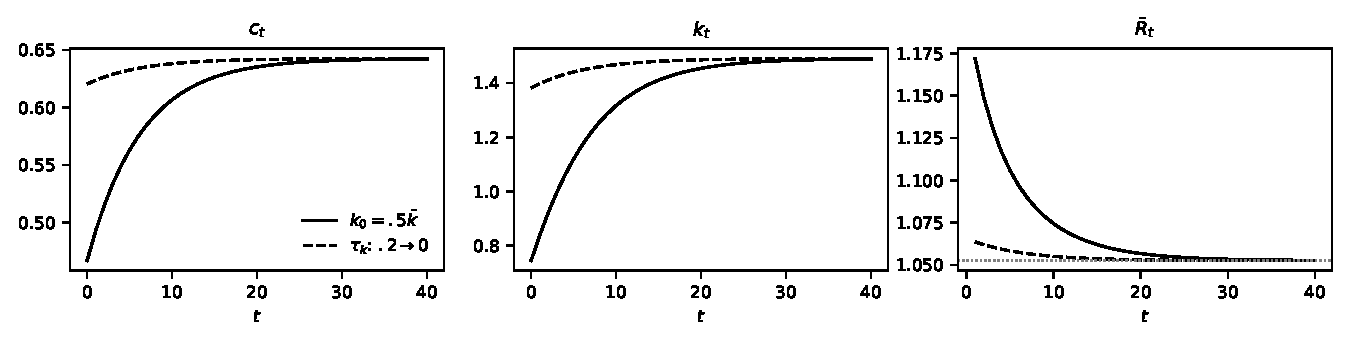
\includegraphics[width=\textwidth]{figures/ch11_11.pdf}\\
{\small Figure S11.7.  Two stories behind Figure \bk{11.1}.}
\end{center}
\end{ex}

%%---------------------------------------------------------------------------
\begin{ex}{11.12}{Reading a falling consumption path}
\textbf{(a)}  Three principles apply.  (i) Under perfect foresight, consumption reacts to news when it arrives, and foreseen policy changes affect
consumption before they occur.  The flat path before $t=12$ therefore means that until $t=12$ households expected policy to stay constant and the economy was
in a steady state.  Whatever happens at $t=12$ was unforeseen.  (ii) A jump in consumption at $t=12$ signals news at $t=12$.  (iii) After $t=12$ consumption
declines smoothly to a lower level, so $\bar R_t<1+\rho$ during the decline and returns to $1+\rho$.  In the long run, private consumption is lower, which
requires a permanently higher $g$ and/or a permanently higher $\tau_k$.

\emph{Story A} (our main story).  At $t=12$ the government unexpectedly and permanently raises $g$ and finances it partly with a permanently higher capital tax,
with lump-sum taxes balancing the budget.  From then on the new policy is foreseen correctly.  On impact, consumption falls by $\Delta g$, less the upward
jump caused by the incentive to run down capital (exercise 11.7(b)).  It then declines along the saddle path to $\bar c'=f(\bar k')-\delta\bar k'-\bar g-\Delta g$.
With $g$ rising from $.2$ to $.23$ and $\tau_k$ from $0$ to $.3$, consumption drops from $0.6426$ to $0.6355$ at $t=12$ and then declines, convexly, to $0.6013$
(Figure S11.8, solid lines).  The relative size of the drop and of the later decline depends on the relative size of the two policy changes.

\textbf{(b)}  Under story A, $g_t=\bar g$ until $t=11$ and is permanently higher from $t=12$.  Capital is constant at $\bar k$ until $t=12$ and then falls
monotonically to $\bar k'=1.311$, where $f'(\bar k')=\delta+\rho/(1-\tau_k)$.  $\bar R_t=1+\rho$ until $t=11$.  The realized return on capital carried into $t=12$
falls to $1+(1-\tau_k)(f'(\bar k)-\delta)=1.0368$: a surprise capital loss, so the Euler equation between $t=11$ and $12$ fails ex post.  Then
$\bar R_{13}=1.0387$, and $\bar R_t$ rises back to $1+\rho$ as capital falls.

\emph{Story B} is also consistent.  At $t=12$ news arrives that $g$ will rise permanently at a later date, say $t=22$, with lump-sum finance.  Consumption drops
at $t=12$ (from $0.643$ to $0.609$) and declines thereafter to $\bar c-\Delta g$.  Capital rises until $t=22$ (to $2.10$) and then falls back to $\bar k$, so
$\bar R_t<1+\rho$ throughout, with its minimum at $t=22$; $g$ is constant until $t=22$.  In story B the decline accelerates until $g$ rises and decelerates
afterwards, an S-shape.  In story A the decline is convex throughout, which is closer to Figure \bk{11.2} (Figure S11.8, dashed lines).
\begin{center}
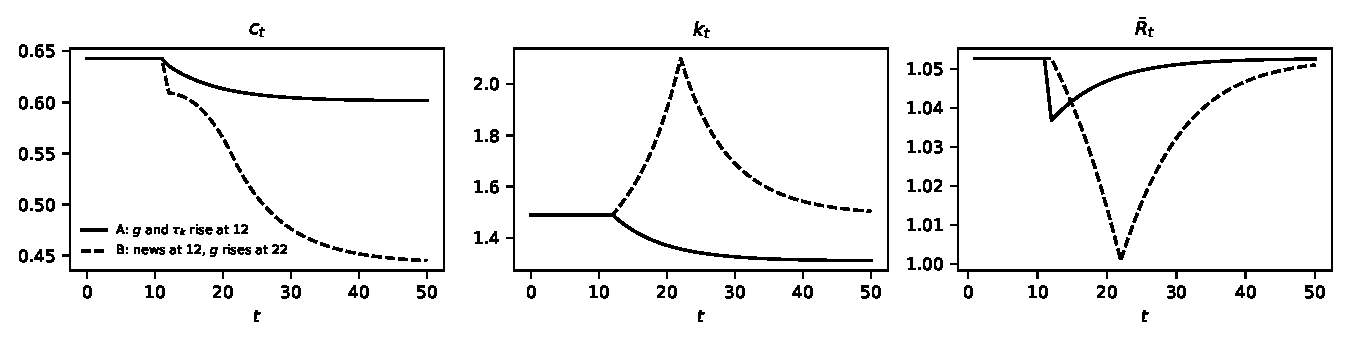
\includegraphics[width=\textwidth]{figures/ch11_12.pdf}\\
{\small Figure S11.8.  Two stories behind Figure \bk{11.2}: A, an unforeseen rise of $g$ ($.2\to.23$) and $\tau_k$ ($0\to.3$) at $t=12$; B, news at $t=12$ that $g$
will rise from $.2$ to $.4$ at $t=22$.}
\end{center}
\end{ex}

%%---------------------------------------------------------------------------
\begin{ex}{11.13}{Linear utility and the saving rate}
\textbf{(a)}  Let $W_t=f(k_t)+(1-\delta)k_t$, so $c_t=W_t-k_{t+1}$ with $0\le k_{t+1}\le W_t$.  Every feasible path is bounded, and summing by parts
gives
\[
  \sum_{t=0}^\infty\beta^tc_t=W_0+\sum_{t=1}^\infty\beta^t\pi(k_t),\qquad \pi(k)\equiv f(k)-(\rho+\delta)k,
\]
because $\beta^t[f(k_t)+(1-\delta)k_t]-\beta^{t-1}k_t=\beta^t\pi(k_t)$ and $\beta^Tk_{T+1}\to0$.  So the planner wants each $k_t$ as close as possible to the
maximizer of the strictly concave $\pi$, which is $\bar k$, where $f'(\bar k)=\rho+\delta$.  The only link between periods is $k_{t+1}\le W_t$.  Let $K_t$ be the
largest attainable capital, $K_0=k_0$ and $K_{t+1}=f(K_t)+(1-\delta)K_t$.  We claim the optimal policy is
\[
  k_{t+1}=\min\{\bar k,\ f(k_t)+(1-\delta)k_t\},\qquad c_t=f(k_t)+(1-\delta)k_t-k_{t+1}.
\]
It generates $k^*_t=\min\{\bar k,K_t\}$ for $t\ge1$, because once $K_t\ge\bar k$ we have $f(\bar k)+(1-\delta)\bar k>\bar k$.  Any feasible path has $k_t\le K_t$.  If
$K_t\le\bar k$, then $\pi(k_t)\le\pi(K_t)=\pi(k^*_t)$, since $\pi$ increases on $[0,\bar k]$; otherwise $\pi(k_t)\le\pi(\bar k)=\pi(k^*_t)$.  So the policy is optimal term by
term, and strict concavity makes it unique.

\textbf{(b)}  If $k_0>\bar k$, the planner eats the excess at once: $c_0=f(k_0)+(1-\delta)k_0-\bar k>\bar c$, and then $k_t=\bar k$ and $c_t=\bar c=f(\bar k)-\delta\bar k$ for $t\ge1$.

\textbf{(c)}  If $k_0<\bar k$ but $f(k_0)+(1-\delta)k_0\ge\bar k$, then $k_1=\bar k$ with $c_0=f(k_0)+(1-\delta)k_0-\bar k\in[0,\bar c)$, and the steady state follows.
Otherwise the planner consumes nothing and invests everything ($c_t=0$, $k_{t+1}=K_{t+1}$) until $\bar k$ becomes reachable; in that period it consumes the
surplus above $\bar k$, and from then on it stays at $\bar k$.  With linear utility there is no smoothing motive, so adjustment is ``bang-bang'' and as fast as
possible: this is the case $\gamma=0$, $\lambda_2=0$, of section \bk{11.10.6}.

\textbf{(d)}  From the policy, $s(k)=[k_{t+1}-(1-\delta)k]/f(k)$, so
\[
  s(k)=\min\Bigl\{1,\ \frac{\bar k-(1-\delta)k}{f(k)}\Bigr\}.
\]
It equals $1$ for small $k$, when $f(k)+(1-\delta)k\le\bar k$.  Where it is interior it is strictly decreasing: its derivative has the sign of
$-(1-\delta)f(k)-[\bar k-(1-\delta)k]f'(k)$, which is negative when $\bar k\ge(1-\delta)k$.  When $\bar k<(1-\delta)k$ the sign is that of
$(1-\delta)[kf'(k)-f(k)]-\bar kf'(k)<0$, because $kf'(k)<f(k)$.  At the steady state, $s(\bar k)=\delta\bar k/f(\bar k)$, which equals $\alpha\delta/(\rho+\delta)$ for
Cobb--Douglas.  The saving rate is negative (gross disinvestment) for $k>\bar k/(1-\delta)$, and it tends to $-\infty$ as $k\to\infty$ since $f(k)/k\to0$.  With
the chapter's parameters, $s=1$ for $k\le0.734$ ($=.49\bar k$), $s(\bar k)=0.261$, and $s<0$ for $k>1.862$.  Figure S11.9 compares this kinked rule with the optimal saving
rates for CRRA utility: they are flatter, and they approach the linear-utility rule as $\gamma\to0$.
\begin{center}
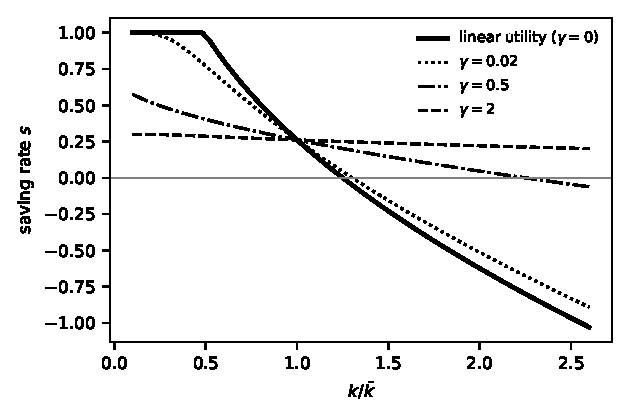
\includegraphics[width=0.5\textwidth]{figures/ch11_13.pdf}\\
{\small Figure S11.9.  Saving rate $s=[k_{t+1}-(1-\delta)k_t]/f(k_t)$ as a function of $k_t$: linear utility and CRRA utility ($g=0$).}
\end{center}
\end{ex}

%%---------------------------------------------------------------------------
\begin{ex}{11.14}{Transitions with and without government purchases}
\textbf{(a)}  The household maximizes $\sum_t\beta^tu(c_t)$ subject to
\[
  \sum_tq_t[(1+\tau_{ct})c_t+k_{t+1}-(1-\delta)k_t]\le\sum_tq_t[\eta_tk_t-\tau_{kt}(\eta_t-\delta)k_t+w_t-\tau_{ht}],
\]
$k_0$ given.  The firm maximizes $\sum_tq_t[f(k_t)-\eta_tk_t-w_t]$ per worker.  The government satisfies
$\sum_tq_tg_t=\sum_tq_t[\tau_{ct}c_t+\tau_{kt}(\eta_t-\delta)k_t+\tau_{ht}]$.  A competitive equilibrium is a budget-feasible policy, a feasible allocation
($c_t+g_t+k_{t+1}=f(k_t)+(1-\delta)k_t$) and a price system such that, given prices and policy, the allocation solves the household's and the firm's problems.
It is characterized by (E), feasibility and the terminal condition.

\textbf{(b)}  $f'(\bar k)=\rho+\delta$, so $\bar k=[\alpha z/(\rho+\delta)]^{1/(1-\alpha)}$.  The steady-state saving rate is $\bar x/f(\bar k)=\delta\bar k/f(\bar k)$, which
for Cobb--Douglas ($f(\bar k)/\bar k=(\rho+\delta)/\alpha$) equals $\alpha\delta/(\rho+\delta)=0.261$ with the chapter's parameters.

\textbf{(c)}  As in exercise 11.6(b): $k$ rises monotonically from $0.745$ to $1.490$, $c$ rises from $0.648$ to $0.843$, and $\bar R_{t+1}$ falls from $1.166$ to
$1.0526$ (Figure S11.10, solid lines; $\gamma=2$).

\textbf{(d)}  We take $\varphi=.1$, so $\bar g=0.0907$.  \emph{Identical:} the steady-state capital stock and the steady-state return, since $\bar g$ does not enter
$f'(\bar k)=\rho+\delta$, and the fact that the timing of the lump-sum taxes is irrelevant.  \emph{Different:} steady-state consumption is lower by $\bar g$, and the
whole transition differs.  Consumption is lower (at $t=0$, $0.565$ instead of $0.648$, a fall smaller than $\bar g$, so investment also falls: $k_1=0.848$ instead of
$0.856$).  Capital converges more slowly ($\lambda_2=0.840$ instead of $0.830$; $k_{10}=1.343$ instead of $1.360$), so $\bar R$ stays high longer (dashed lines).
The reason: in terms of total absorption $C_t=c_t+\bar g$, the planner maximizes $\sum_t\beta^tu(C_t-\bar g)$, a Stone--Geary utility whose curvature
$-Cu''/u'=\gamma C/(C-\bar g)$ exceeds $\gamma$.  Government purchases act like a subsistence requirement, which makes the household less willing to substitute
consumption over time, so, as with a higher $\gamma$, the transition is slower.  Only with linear utility would the capital paths coincide.

\textbf{(e)}  \emph{Algorithm.}  For a trial $\bar\tau_k$: (i) the terminal steady state solves $f'(\bar k)=\delta+\rho/(1-\bar\tau_k)$; (ii) solve for the equilibrium
path from $k_0$ (by shooting or Newton's method), using (E) with $\bar R_{t+1}=1+(1-\bar\tau_k)(f'(k_{t+1})-\delta)$ and feasibility with $g_t=\bar g$; (iii) compute
$q_t=\beta^tu'(c_t)/u'(c_0)$ and the present-value surplus
\[
  \Gamma(\bar\tau_k)=\sum_tq_t\bar\tau_k\bigl(f'(k_t)-\delta\bigr)k_t-\bar g\sum_tq_t ;
\]
(iv) solve $\Gamma(\bar\tau_k)=0$ by bisection or the secant method, taking the smallest root if there are several (Laffer curve).  An equilibrium exists only if
$\bar g$ is small enough.  For Cobb--Douglas, $(f'(k)-\delta)k=\alpha f(k)-\delta k$, so revenue per period can never exceed $\max_k[\alpha f(k)-\delta k]=0.164$.
With $\varphi=.2$ ($\bar g=0.181$) no equilibrium would exist.  With $\varphi=.1$, $\Gamma$ increases on $[.05,.95]$ and its root is $\bar\tau_k=0.641$.  The steady
state is then $k=0.929$, $c=0.699$, and capital rises only slowly from $0.745$ (dash-dotted lines).  The government runs primary surpluses early, when the tax
base $\alpha f(k)-\delta k$ is large, and a small primary deficit in the long run (revenue $0.087<\bar g$), financed by interest on the assets it has
accumulated.
\begin{center}
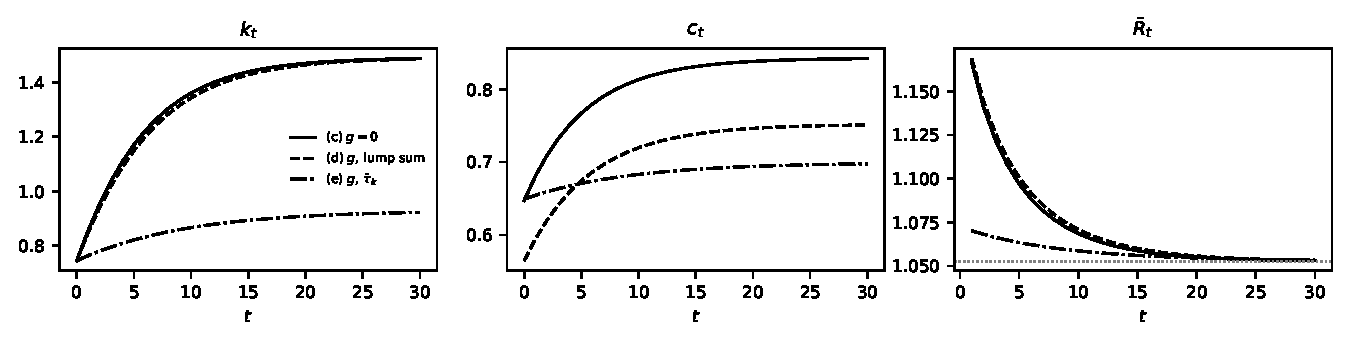
\includegraphics[width=\textwidth]{figures/ch11_14.pdf}\\
{\small Figure S11.10.  Transitions from $k_0=.5\bar k$: (c) $g=0$; (d) $\bar g=.1f(k_0)$ with lump-sum taxes; (e) the same $\bar g$ financed by $\bar\tau_k=0.641$.}
\end{center}
\end{ex}

%%---------------------------------------------------------------------------
\begin{ex}{11.15}{Reading the yield curve}
Assume a constant consumption tax (or none).  Then $r_{t,t+1}=\log(q_t/q_{t+1})=-\log\beta+\gamma\log(c_{t+1}/c_t)=\log\bar R_{t+1}$.  Since $r_{0,t}$ is the
average of the first $t$ short rates, an increasing $r_{0,t}$ means the short rates increase, and a flattening curve means they converge.  If policy is
eventually constant, rates converge to the steady-state rate $\log(1+\rho)$ \bk{(11.6.10)}.  So the short rates are below $\log(1+\rho)$ and rising, and
consumption falls at a decreasing rate, $c_{t+1}/c_t=(\beta\bar R_{t+1})^{1/\gamma}<1$, approaching its steady state from above.  With a constant capital tax,
$\bar R_{t+1}<1+\rho$ means $f'(k_{t+1})<\delta+\rho/(1-\tau_k)$: capital is above its steady state and falling.  The smooth concave curve points to pure
transient dynamics.  A foreseen future policy change would bend the curve, as in the U-shaped curve of Figure \bk{11.9.3}.

Stories that fit: (i) the unforeseen permanent increase of the capital tax at $t=0$ of exercise 11.10(d), with lump-sum rebates, for which $r_{0,t}$ rises
from $0.0426$ at $t=1$ to $0.0463$ at $t=10$ and $0.0497$ at $t=40$; (ii) more generally, constant policy and an economy that starts with more capital than
its steady state.  With $k_0=1.5\bar k$, $r_{0,t}$ rises from $0.000$ to $0.042$ at $t=40$ (Figure S11.11).
\begin{center}
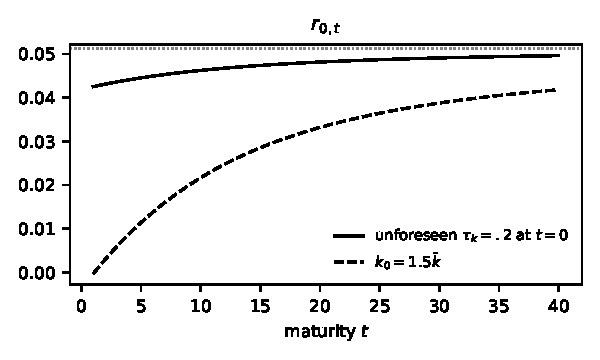
\includegraphics[width=0.5\textwidth]{figures/ch11_15.pdf}\\
{\small Figure S11.11.  Upward-sloping, concave yield curves at $t=0$; dotted: $\log(1+\rho)$.}
\end{center}
\end{ex}

%%---------------------------------------------------------------------------
\begin{ex}{11.16}{Low versus high $\gamma$}
The steady state, $f'(\bar k)=\delta+\rho/(1-\tau_k)$, does not involve $\gamma$, so both economies converge to the same $\bar k$ (the dashed line at
$\rho+\delta$ in Figure \bk{11.5} shows $\tau_k=0$).  The speed of convergence is $\lambda_2$, which increases with $\gamma$.  A household with low $\gamma$ has a
high intertemporal elasticity $1/\gamma$: when $k_0<\bar k$ it accepts very low consumption now in order to exploit the high return on capital, so capital
converges quickly.

\textbf{(a)}  Panel (b), where capital jumps to the steady state almost at once, is the low-$\gamma$ economy; panel (a), with gradual convergence, is the
high-$\gamma$ economy.

\textbf{(b)}  $f'(k_t)$ mirrors $k_t$, because $f'$ is decreasing.  Panel (b), with its fast decline to $\rho+\delta$, is the low-$\gamma$ economy; panel (a) is
the high-$\gamma$ one.

\textbf{(c)}  By (E), $c_{t+1}/c_t=(\beta\bar R_{t+1})^{1/\gamma}$: for a given return above $1+\rho$, consumption grows faster the lower is $\gamma$.  In equilibrium
the low-$\gamma$ household starts from much lower consumption and catches up quickly; the high-$\gamma$ household's path is smoother and slower.  With
$k_0=.5\bar k$ and the chapter's parameters (Figure S11.12): for $\gamma=.2$, $\lambda_2=0.578$, $c_0=0.295$, $c_5=0.614$, and capital is within $1\%$ of $\bar k$ after
8 periods; for $\gamma=2$, $\lambda_2=0.852$, $c_0=0.467$, $c_5=0.563$, and it takes 26 periods.  Both paths converge to $\bar c=0.643$.  (With $\tau_k>0$ the
capital-tax revenue differs along the two paths, so the lump-sum taxes that balance the budget differ, as the book's footnote notes; the allocation does not
depend on their timing.)
\begin{center}
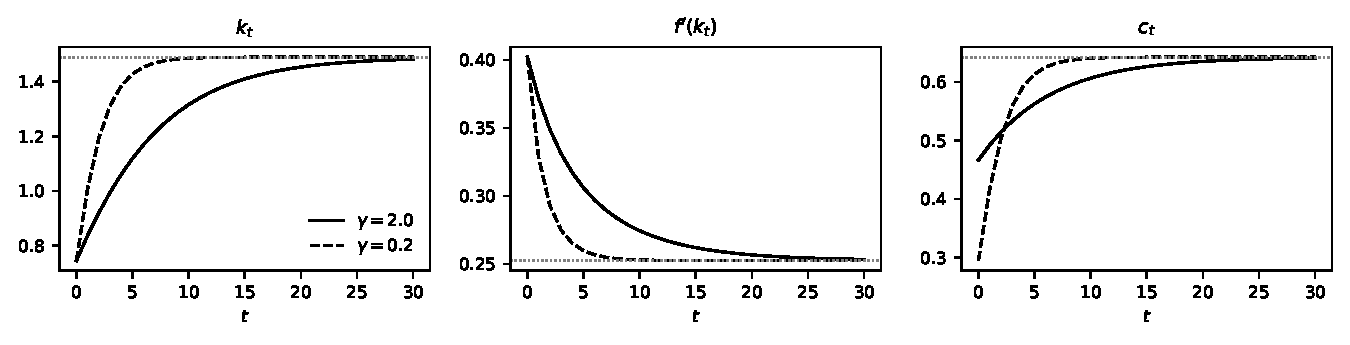
\includegraphics[width=\textwidth]{figures/ch11_16.pdf}\\
{\small Figure S11.12.  Low ($\gamma=.2$) versus high ($\gamma=2$) curvature, from $k_0=.5\bar k$ ($g=.2$, no distorting taxes).}
\end{center}
\end{ex}

%%---------------------------------------------------------------------------
\begin{ex}{11.17}{Anticipated versus unanticipated government purchases}
Panel (a), where consumption is constant at $0.643$ until $t=9$ and constant at $0.443$ from $t=10$, is the unanticipated jump.  Panel (b), where consumption
declines smoothly from $t=0$, is the anticipated one.

\emph{Unanticipated.}  Until $t=10$ households expect $g=.2$ forever, so the economy stays in its steady state ($k_t=\bar k$, $c_t=\bar c$, $\bar R_t=1+\rho$).
At $t=10$ they learn that $g=.4$ forever.  Since $g$ does not enter $f'(\bar k)=\rho+\delta$ and $k_{10}=\bar k$, the new equilibrium is $k_t=\bar k$ and
$c_t=\bar c-.2=0.443$ for all $t\ge10$ (exercise 11.5(c)).  Consumption falls by exactly the increase in $g$, and capital and the interest rate never move.

\emph{Anticipated.}  At $t=0$ the present value of lump-sum taxes rises, so consumption falls at once, to $0.609$, and keeps falling.  Households build up
capital before $t=10$, to $k_{10}=2.098$, to smooth consumption, and run it down afterwards.  Because $k_t>\bar k$ for all $t\ge1$,
$\bar R_t=1-\delta+f'(k_t)<1+\rho$ throughout; this is what makes a declining consumption path optimal.  $\bar R_t$ reaches its minimum, $1.0008$, at $t=10$, when
capital peaks, and then rises back to $1+\rho$.  The time-0 yield curve is U-shaped, as in Figure \bk{11.9.3}.

Figure S11.13 reproduces Figure \bk{11.6}.  Cross-checks: the book's shooting algorithm gives $c_0=0.609242$, the same as Newton's method to $5\times10^{-10}$.  The
linear approximation \bk{(11.10.8)} around the terminal steady state, with $\lambda_2=0.879$ and $\lambda_1=1.197$ ($\beta\lambda_1\lambda_2=1$), gives
$k_{10}=2.090$ and stays within $0.015$ of the nonlinear path.
\begin{center}
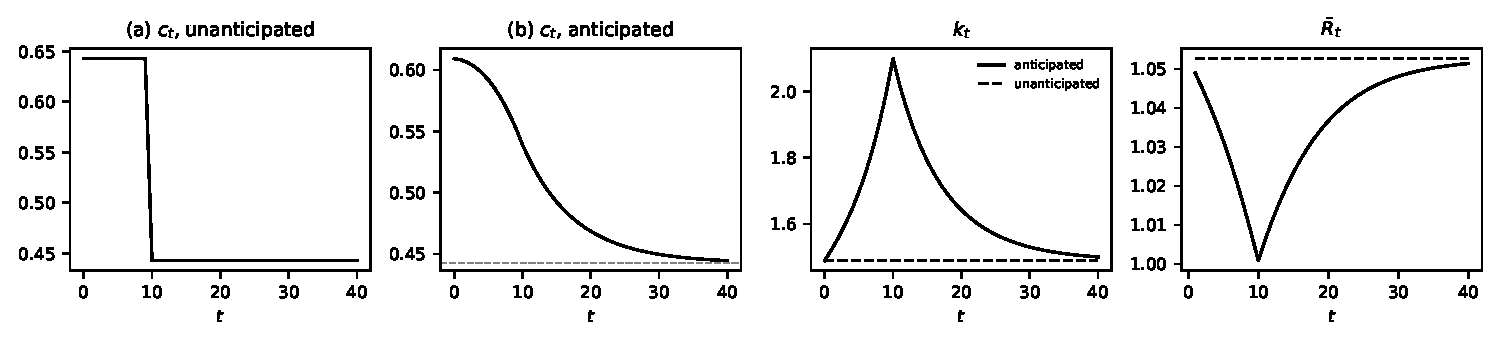
\includegraphics[width=\textwidth]{figures/ch11_17.pdf}\\
{\small Figure S11.13.  An unanticipated and an anticipated jump of $g$ from $.2$ to $.4$ at $t=10$ ($\gamma=2$).}
\end{center}
\end{ex}

%%---------------------------------------------------------------------------
\begin{ex}{11.18}{Habit persistence and durability}
\rmk{The exercise states $\lim_{c\downarrow0}u'(c)=0$; for CRRA utility, and for the usual Inada condition, the limit is $+\infty$.}

\textbf{(a)}  Let $x_t=c_t-\alpha c_{t-1}$, and attach $\beta^t\mu_t$ to the time-$t$ resource constraint.  The first-order conditions are
\[
  \mu_t=u'(x_t)-\alpha\beta u'(x_{t+1}),\qquad \mu_t=\beta\mu_{t+1}\bigl[f'(k_{t+1})+1-\delta\bigr],\qquad \lim_{t\to\infty}\beta^t\mu_tk_{t+1}=0,
\]
together with feasibility, $x_t>0$ and the initial conditions.  The first condition says that consuming more today raises today's utility, but it also
raises tomorrow's habit ($\alpha>0$) or tomorrow's services ($\alpha<0$).  Eliminating $\mu$ gives a third-order difference equation in $c$ (fourth-order in
$k$):
\[
  u'(x_t)-\alpha\beta u'(x_{t+1})=\beta[f'(k_{t+1})+1-\delta]\bigl[u'(x_{t+1})-\alpha\beta u'(x_{t+2})\bigr].
\]

\textbf{(b)}  An optimal steady state is a constant triple $(k,c,\mu)$ that satisfies these conditions: if $(k_0,c_{-1})=(k,c)$, the optimal path stays there.

\textbf{(c)}  A constant $\mu>0$ requires $1=\beta[f'(k)+1-\delta]$, so
\[
  f'(k)=\rho+\delta,\qquad c=f(k)-\delta k,\qquad \mu=(1-\alpha\beta)\,u'\bigl((1-\alpha)c\bigr)>0 .
\]
The steady state does not depend on $\alpha$: habits and durability shape the dynamics, not the long run.  With the chapter's technology, $k=1.490$,
$f'(k)=0.2526$ and $c=0.843$.

\textbf{(d)}  The state is $(k_t,c_{t-1})$: two predetermined variables.  Linearized, the fourth-order equation has four roots.  Because the problem is a
planning problem they come in pairs $(\lambda,1/(\beta\lambda))$: two stable and two unstable roots.  So the two initial conditions and the requirement to
converge pin down a unique path.

\emph{Algorithm} (implemented in \texttt{ch11.py}).  1. Compute the steady state of (c).  2. Choose a large $S$, take $k_1,\dots,k_{S-1}$ as unknowns, and set
$k_t=k$ for $t\ge S$ (so $c_t=c$ for $t\ge S$).  3. Given the unknowns, compute $c_t$ from feasibility, $x_t=c_t-\alpha c_{t-1}$ using the given $c_{-1}$, and
$\mu_t$ from the first condition.  4. Solve the $S-1$ Euler equations $\mu_t=\beta\mu_{t+1}[f'(k_{t+1})+1-\delta]$ by Newton's method; the Jacobian is banded,
since each equation involves $k_{t-1},\dots,k_{t+3}$.  5. Check that the solution does not change when $S$ grows, and that $x_t>0$ and $\mu_t>0$.  A shooting
alternative guesses $(c_0,c_1)$, iterates forward (for $k_{t+1}$ from feasibility, $\mu_{t+1}$ from the Euler equation, and then $x_{t+2}$ from the first condition), and
adjusts the two guesses by a two-dimensional Newton method until $(k_S,c_S)=(k,c)$; it becomes inaccurate for long horizons, as does all shooting.  The linear
approximation solves the two stable roots backward and the two unstable roots forward.

\emph{Results} ($\gamma=2$, $k_0=.5k$, $c_{-1}=c$; Figure S11.14).  For $\alpha=.5$ the stable roots are $0.516$ and $0.822$, for $\alpha=-.5$ they are $-0.487$ and
$0.831$, and each root times its unstable partner equals $1/\beta=1.0526$.  The computed paths converge at the dominant stable root, and for $\alpha=0$ the
algorithm reproduces the standard model's path to $10^{-15}$.  With a habit, low consumption relative to last period's $c_{-1}$ is painful, so the planner cuts
consumption gradually ($c_0=0.734$, against $0.648$ without habit) and accumulates capital more slowly.  With durability, the stock inherited from $c_{-1}$
still provides services, so purchases fall more at $t=0$ ($c_0=0.565$) and capital is built faster.  The negative root makes purchases of the durable
oscillate.
\begin{center}
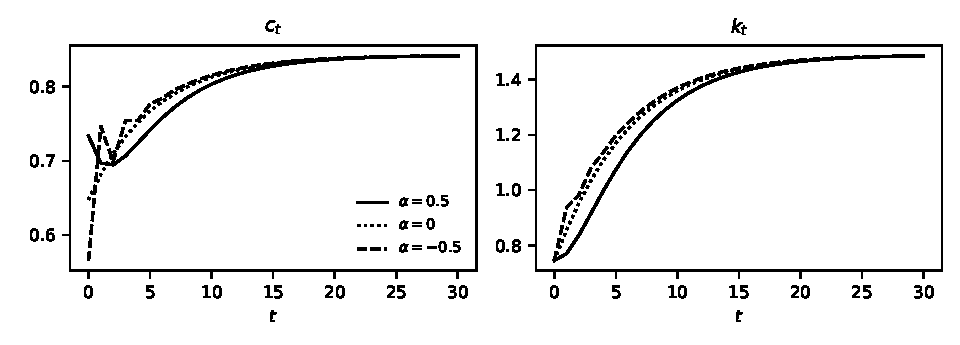
\includegraphics[width=0.66\textwidth]{figures/ch11_18.pdf}\\
{\small Figure S11.14.  Optimal paths with habit ($\alpha=.5$), without ($\alpha=0$) and with durability ($\alpha=-.5$), from $k_0=.5k$ and $c_{-1}=c$.}
\end{center}
\end{ex}

%%---------------------------------------------------------------------------
\begin{ex}{11.19}{The invisible hand, I}
\textbf{(a)}  The household takes as given the price system: $\{q_t\}$ (equivalently the interest rates $R_{t,t+1}=q_t/q_{t+1}$, i.e.\ the whole yield curve),
the rental rates $\{\eta_t\}$ and the wages $\{w_t\}$.  It also takes as given the tax plan: lump-sum taxes $\{\tau_{ht}\}$, of which only the present value
matters, and zero distorting taxes.  Its own initial capital $k_0$ is an endowment, not a market signal.  The household does not care about $g_t$ as such; the
increase in $g$ reaches it only through taxes and prices.  After the announcement: the present value of lump-sum taxes rises from $4.00$ to $9.79$ (time-0
goods); interest rates fall below $\rho=0.0526$ and follow a U-shaped path ($R_{t,t+1}-1=0.049$ at $t=0$, $0.026$ at $t=5$, $0.0008$ at $t=9$, $0.006$ at
$t=10$, $0.038$ at $t=20$); and wages and rental rates move with aggregate capital.

\textbf{(b)}  Big $K$ is the aggregate path.  Shooting (or Newton's method) is applied to the aggregate conditions
$u'(C_t)=\beta u'(C_{t+1})[f'(K_{t+1})+1-\delta]$ and $K_{t+1}=f(K_t)+(1-\delta)K_t-g_t-C_t$, with $K_0=\bar k$ and $K_S\approx\bar k$.  This gives $\{C_t,K_t\}$, and
then $\eta_t=f'(K_t)$, $w_t=f(K_t)-K_tf'(K_t)$, $q_t=\beta^tu'(C_t)/u'(C_0)$, and lump-sum taxes with $\sum_tq_t\tau_{ht}=\sum_tq_tg_t$ (for instance
$\tau_{ht}=g_t$).

\textbf{(c)}  The household maximizes $\sum_t\beta^tu(c_t)$ subject to $\sum_tq_t[c_t+k_{t+1}-(1-\delta)k_t]\le\sum_tq_t(\eta_tk_t+w_t-\tau_{ht})$.  Because
prices satisfy no-arbitrage, $q_t=q_{t+1}(\eta_{t+1}+1-\delta)$, capital drops out and the budget becomes
\[
  \sum_tq_tc_t=W_0\equiv(\eta_0+1-\delta)k_0+\sum_tq_t(w_t-\tau_{ht}),\qquad q_0=1:
\]
the household is indifferent about how much capital it holds, as long as the budget holds.  Its first-order condition $\beta^tu'(c_t)=\mu q_t$ gives
\[
  c_t=c_0\,(q_t/\beta^t)^{-1/\gamma},\qquad c_0=\frac{W_0}{\sum_tq_t(q_t/\beta^t)^{-1/\gamma}} .
\]
Two forces are at work.  A wealth effect: taxes are higher, and at the new prices the old plan ($c_t=0.643$ forever) would cost $18.47$, more than
$W_0=14.50$.  A substitution effect: interest rates below $1/\beta-1$ tilt consumption downward over time, $c_{t+1}/c_t=(\beta R_{t,t+1})^{1/\gamma}<1$.  So the
household cuts consumption at once, to $0.609$, and plans a declining path.  With $\tau_{ht}=g_t$, it invests the difference between income and consumption
in capital.

\textbf{(d)}  Guess $c_0$.  Generate $c_{t+1}=c_t(\beta R_{t,t+1})^{1/\gamma}$ from the given interest rates and $k_{t+1}=(\eta_t+1-\delta)k_t+w_t-\tau_{ht}-c_t$
from the budget.  If $k_S$ ends above its target (the terminal condition $\lim q_Tk_{T+1}=0$, here $K_S$), $c_0$ was too low: raise it; otherwise lower it.
Since prices are given, this is a linear problem, and bisection converges to machine precision.  Numerically the household's $c_0=0.60924195$ equals $C_0$,
the budget formula of (c) gives the same value, and $\max_t|c_t-C_t|=3\times10^{-14}$, $\max_t|k_t-K_t|=2\times10^{-13}$ for $t\le100$.

\textbf{(e)}  Check that the household's optimal choice, given the prices computed from Big $K$, is Big $K$ itself: $c_t=C_t$, $k_t=K_t$.  Indeed $C_t$
satisfies $u'(C_t)=\beta u'(C_{t+1})R_{t,t+1}$ with $R_{t,t+1}=f'(K_{t+1})+1-\delta$, which is the household's Euler equation.  With $k_t=K_t$ and $\tau_{ht}=g_t$ the
household's budget gives $k_{t+1}=f'(K_t)K_t+(1-\delta)K_t+f(K_t)-K_tf'(K_t)-g_t-C_t=K_{t+1}$.  So individual optimization reproduces the aggregate path that
generated the prices, and that fixed point is the competitive equilibrium.
\end{ex}

%%---------------------------------------------------------------------------
\begin{ex}{11.20}{The invisible hand, II}
We use the parameters of section \bk{11.9} ($\alpha=.33$, $\delta=.2$, $\beta=.95$, $g=.2$), $B=3$, and a rise of $\tau_n$ from $0$ to $.2$; these reproduce
Figure \bk{11.12.3} (Figure S11.15).  The steady states have $k/n=\tilde k=1.490$ and $w=\bar w=0.764$ both before and after, with
$(c,n,k)=(0.2547,0.540,0.804)$ before and $(0.2038,0.479,0.714)$ after.

\textbf{(a)}  The household takes as given the prices $\{q_t,\eta_t,w_t\}$, the labor tax rates $\{\tau_{nt}\}$ ($0$ before $t=10$, $.2$ after), zero
consumption and capital taxes, and the lump-sum taxes, which here are transfers rebating the labor-tax revenue (only their present value matters).  The signals
that matter are the after-tax wage $(1-\tau_{nt})w_t$ and the interest rates $R_{t,t+1}=q_t/q_{t+1}=1+f'(K_{t+1}/N_{t+1})-\delta$.

\textbf{(b)}  The household maximizes $\sum_t\beta^t[\log c_t+B(1-n_t)]$ subject to
$\sum_tq_tc_t=(\eta_0+1-\delta)k_0+\sum_tq_t[(1-\tau_{nt})w_tn_t-\tau_{ht}]$.  Its first-order conditions $\beta^t/c_t=\mu q_t$ and
$\beta^tB=\mu q_t(1-\tau_{nt})w_t$ give
\[
  c_t=(1-\tau_{nt})w_t/B,\tag{I}
\]
\[
  c_{t+1}/c_t=\beta q_t/q_{t+1}=\beta R_{t,t+1}.\tag{II}
\]
By (I), consumption is tied to the after-tax wage: given prices, it does not depend on wealth.  Substituting $\mu q_t(1-\tau_{nt})w_t=\beta^tB$ into the budget
shows that the value of any labor plan is $\sum_tq_t(1-\tau_{nt})w_tn_t=(B/\mu)\sum_t\beta^tn_t$.  So utility depends on the labor plan only through
$\sum_t\beta^tn_t$, which the budget pins down.  At equilibrium prices the household is therefore indifferent among all labor plans with the same
$\sum_t\beta^tn_t$: its intertemporal labor supply is perfectly elastic (Hansen--Rogerson).  The timing of work is set by the Big $K$ conditions, and small price
changes can support large reallocations of work.  That is why:
\begin{itemize}[leftmargin=*]
\item \emph{Before $t=10$} the capital-labor ratio, and hence $w_t$ and $R_{t,t+1}$, stay almost exactly at their steady-state values ($k/n$ between $1.4848$
and $1.4898$).  By (I) and (II), so does consumption, which stays within $0.12\%$ of $0.2547$.
\item \emph{Work is shifted toward $t<10$.}  From $t=10$ on, the after-tax wage is lower, so leisure is cheaper then.  The household works more before
$t=10$: $n$ rises from $0.540$ to $0.614$ at $t=9$.  Consumption cannot rise, since it is tied to the after-tax wage, so the extra earnings are saved, and
capital rises from $0.804$ to $0.976$ at $t=10$.  At a constant capital-labor ratio, feasibility reads $k_{t+1}=[f(\tilde k)/\tilde k+1-\delta]k_t-g-c_t$, an
explosive equation with root $1.566$.  So a consumption dip of only $0.12\%$ at $t=0$ is amplified into a large build-up of capital and work.
\item \emph{At $t=10$} work falls to $0.409$.  The capital-labor ratio jumps to $2.39$, and the pre-tax wage jumps to $0.893$ ($+17\%$), which partly offsets the
tax: the after-tax wage falls only $6.5\%$, and by (I) so does consumption (to $0.238$).  The high capital-labor ratio lowers the return to
$\bar R_{10}=0.984<1$, which is what (II) requires for consumption to fall.
\item \emph{After $t=10$} the capital accumulated before $t=10$ is run down to finance consumption while people work less.  The capital-labor ratio returns to
$\tilde k$, the wage to $0.764$, consumption to $0.8\times0.2547=0.2038$, and $(n,k)$ to $(0.479,0.714)$.  Along the way $\bar R<1+\rho$, consistent with
declining consumption.
\end{itemize}
Big $K$, little $k$: the prices are computed from the aggregate path, and at those prices the aggregate path satisfies (I), (II) and the budget.  Since the
household is indifferent among labor plans with the same $\sum_t\beta^tn_t$, choosing $(c_t,n_t,k_t)=(C_t,N_t,K_t)$ is optimal for it: the fixed point.
\rmk{The book says that before $t=10$ the capital-labor ratio and consumption stay \emph{equal} to their initial steady-state values.  They cannot be exactly
constant.  By (I), constant consumption would require a constant capital-labor ratio $\tilde k$.  The explosive equation above would then keep $k$ and $n$ at
their old steady-state values until $t=10$: no response at all before $t=10$.  From $t=10$ on the path would be the response to an unforeseen tax increase at
$t=10$, for which $c_{10}/c_9=0.848$ while $\beta\bar R_{10}=0.973$, violating (II) between $t=9$ and $10$, which must hold when the change is foreseen.  The
deviations are tiny, however: $0.12\%$ for consumption and $0.35\%$ for $k/n$.}
\begin{center}
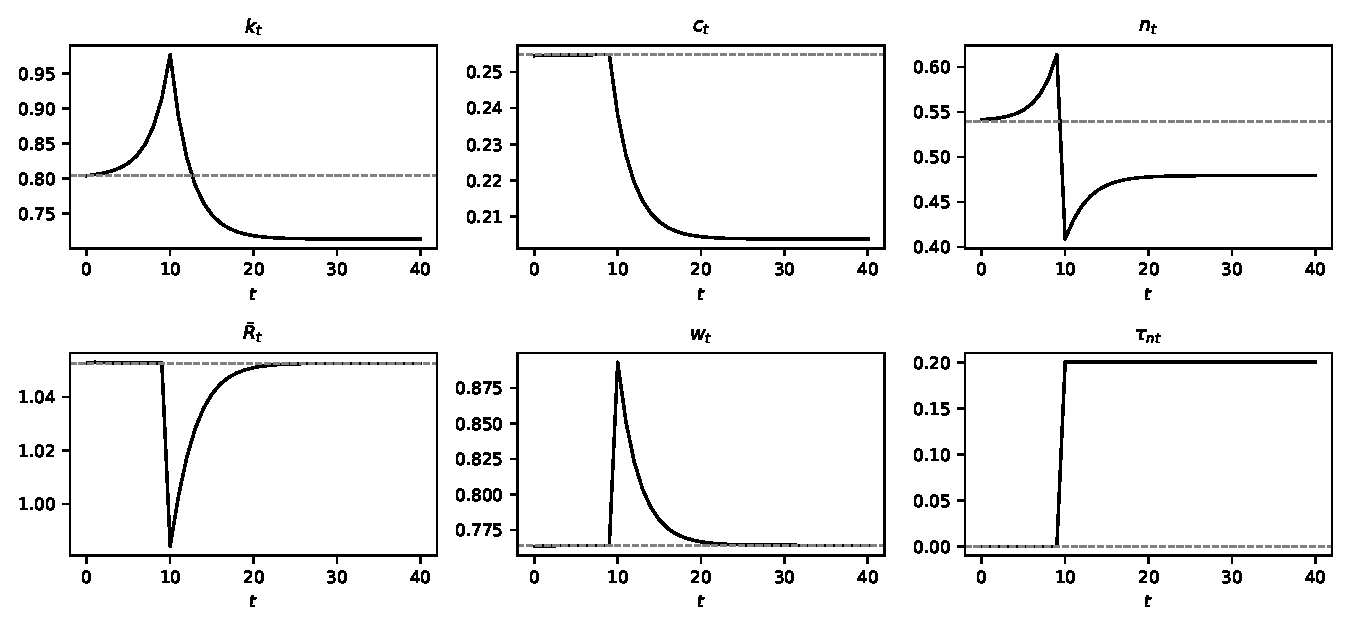
\includegraphics[width=\textwidth]{figures/ch11_20.pdf}\\
{\small Figure S11.15.  Elastic labor supply: a rise of $\tau_n$ from $0$ to $.2$ at $t=10$, foreseen at $t=0$ (compare the book's Figure 11.12.3).  Dashed
lines: the initial steady state.}
\end{center}
\end{ex}

%% ===========================================================================
%% Chapter 13. Asset Pricing Theory
%% ===========================================================================
\solchapter{13}{Asset Pricing Theory}

\begin{center}
\begin{minipage}{0.86\textwidth}
\small
Solutions to all 5 exercises of Chapter 13 of Ljungqvist and Sargent, \emph{Recursive Macroeconomic Theory} (4th edition, 2018).
Numbers come from \texttt{code/ch13.py}, which also recomputes the book's Table 13.A.1 (all six rows are confirmed).
\end{minipage}
\end{center}

\bigskip
\hrule
\bigskip

%%---------------------------------------------------------------------------
\begin{ex}{13.1}{A Markov economy}
\textbf{(a)}  In equilibrium the consumer consumes the endowment, so the price at $t$ (in time-$t$ goods) of one unit of consumption at $t+1$ in state $\bar\lambda_j$,
given $\lambda_t=\bar\lambda_i$, is the marginal rate of substitution times the probability:
\[
  Q_{ij}=\beta P_{ij}\Bigl(\frac{C_{t+1}}{C_t}\Bigr)^{-\gamma}=\beta P_{ij}\bar\lambda_j^{-\gamma}.
\]
Prices depend on the state only through $i$, because utility is homothetic and consumption growth is Markov.  The gross risk-free rate in state $i$ is
$1/\sum_jQ_{ij}$.

\textbf{(b)}  A claim to one unit at $t+2$ in state $j$ costs $\sum_k\beta^2P_{ik}P_{kj}(\bar\lambda_k\bar\lambda_j)^{-\gamma}=(Q^2)_{ij}$.  A claim contingent on the whole path
$(\bar\lambda_k,\bar\lambda_j)$ costs $Q_{ik}Q_{kj}$.  Two-step prices are products of one-step prices, which is why one-step Arrow securities suffice to complete the market.

\textbf{(c)}  The ex-dividend price satisfies $p_t=E_t\bigl[\beta(C_{t+1}/C_t)^{-\gamma}(C_{t+1}+p_{t+1})\bigr]$.  Guess $p_t=v(\lambda_t)C_t$: the price-dividend ratio depends only on the growth
state.  Substituting and dividing by $C_t$,
\[
  v_i=\sum_j\beta P_{ij}\bar\lambda_j^{1-\gamma}(1+v_j),\qquad\text{i.e.}\qquad v=\tilde Q(\mathbf1+v),\quad \tilde Q_{ij}\equiv\beta P_{ij}\bar\lambda_j^{1-\gamma}=Q_{ij}\bar\lambda_j .
\]
Hence
\[
  v=(I-\tilde Q)^{-1}\tilde Q\,\mathbf1=\sum_{k\ge1}\tilde Q^k\mathbf1,\qquad p(C,\bar\lambda_i)=v_iC,
\]
where $(I-\tilde Q)^{-1}$ is the resolvent operator.  It is well defined when the spectral radius of $\tilde Q$ is below one, a growth-adjusted discounting condition.
(Illustration, \texttt{ch13.py}: $\beta=.95$, $\gamma=2$, $\bar\lambda=(.97,1.05)$, $P=\begin{bmatrix}.6&.4\\.2&.8\end{bmatrix}$ give $v=(13.84,13.14)$, and iterating $v\leftarrow\tilde Q(\mathbf1+v)$
reproduces it.)

\textbf{(d)}  The option's value depends on the level of the tree's price, $v_iC$, relative to the fixed strike, so its state is $(C,\lambda)$.  At the start of a period the owner
either exercises, receiving $v(\lambda)C-\check p$, or waits:
\[
  w(C,\bar\lambda_i)=\max\Bigl\{v_iC-\check p,\;\sum_jQ_{ij}\,w(\bar\lambda_jC,\bar\lambda_j)\Bigr\}.
\]
Algorithm: put $C$ on a lattice closed under multiplication by the $\bar\lambda_j$ (e.g.\ a geometric grid when the $\bar\lambda$'s are powers of a common factor), truncated far
from the region where exercise is marginal.  Stack $w$ into a vector $\mathbf w$ indexed by $(C,\lambda)$ and let $\mathcal Q$ be the matrix with element $Q_{ij}$ in position
$\bigl((C,i),(\bar\lambda_jC,j)\bigr)$.  Then iterate
$\mathbf w_{k+1}=\max\{\mathbf g,\mathcal Q\mathbf w_k\}$ (elementwise), with $\mathbf g$ the exercise payoffs, from $\mathbf w_0=\max\{\mathbf g,0\}$.  At the fixed point, the option is exercised in the states where
$\mathbf w=\mathbf g$.

\textbf{(e)}  Let $(Tw)(C,i)=\max\{v_iC-\check p,\ \sum_jQ_{ij}w(\bar\lambda_jC,j)\}$.  Because payoffs grow with $C$, use the weighted sup norm $\|w\|=\sup|w(C,i)|/(1+C)$.  Then:
(i) \emph{monotonicity}: $w\le w'$ implies $Tw\le Tw'$, because $Q_{ij}\ge0$ and $\max$ is monotone;
(ii) \emph{discounting}: for $a\ge0$,
\[
  T\bigl(w+a(1+C)\bigr)(C,i)\le Tw(C,i)+a\sum_jQ_{ij}(1+\bar\lambda_jC)\le Tw(C,i)+a\kappa(1+C),
\]
with $\kappa=\max_i\max\{\sum_jQ_{ij},\sum_j\tilde Q_{ij}\}$.  If $\kappa<1$ (positive risk-free rates and a finite tree price, with row sums of $\tilde Q$ below one), Blackwell's
sufficient conditions, in their weighted form, make $T$ a contraction with modulus $\kappa$.  So the iterations converge to the unique fixed point from any starting value.  On a
truncated $C$-grid the plain sup norm works with modulus $\max_i\sum_jQ_{ij}$.
\end{ex}

%%---------------------------------------------------------------------------
\begin{ex}{13.2}{A Harrison--Kreps asset market}
The rows of the table below are: $p_h=\beta(I-\beta P_h)^{-1}P_hd$ (homogeneous beliefs, \bk{(13.A.1)}); $p$ solving \bk{(13.A.2)} (the optimist prices the asset); the reservation
prices $\hat p_h(s)=\beta P_h(s,\cdot)(d+p)$ that type $h$ would pay given resale at $p$ (the book's rows 4--5); and $\check p$ solving \bk{(13.A.4)} (the pessimist prices it).
As a check, the program reproduces all six rows of the book's Table \bk{13.A.1} exactly.
\begin{center}
\begin{tabular}{lcccc}
\toprule
 & \multicolumn{2}{c}{(a)} & \multicolumn{2}{c}{(b)}\\
$s_t$ & 1 & 2 & 1 & 2\\
\midrule
$p_a$ & $1.263$ & $1.105$ & $1.500$ & $1.500$\\
$p_b$ & $0.923$ & $1.154$ & $0.800$ & $0.867$\\
$p$ (optimists) & $1.500$ & $1.500$ & $1.500$ & $1.500$\\
$\hat p_a$ & $1.500$ & $1.313$ & $1.500$ & $1.500$\\
$\hat p_b$ & $1.313$ & $1.500$ & $1.313$ & $1.375$\\
$\check p$ (pessimists) & $0.750$ & $0.750$ & $0.800$ & $0.867$\\
\bottomrule
\end{tabular}
\end{center}
\textbf{(a)}  Optimism alternates, as in the book.  In state 1, type $a$ assigns probability $\frac12$ to the dividend state versus $b$'s $\frac14$; in state 2 the roles reverse.  So $a$ holds
the asset in state 1 and $b$ in state 2, and the asset changes hands whenever the state changes.  The optimists' price $p=(1.5,1.5)$ exceeds \emph{both} fundamental
valuations in \emph{both} states ($1.5>1.263,\,0.923$ in state 1 and $1.5>1.105,\,1.154$ in state 2): a speculative bubble in the sense of Harrison and Kreps and
Scheinkman, driven by the option to resell to the other type.  The pessimists' price $0.75$ is below both fundamental values.

\textbf{(b)}  Now type $a$ is the optimist in \emph{both} states: it assigns $\frac12$ to the high-dividend state, while $b$ assigns $\frac14$ or $\frac13$.  Type $a$ always holds the asset, there is never
anyone to resell to at a higher valuation, and the resale option is worthless.  Hence $p=p_a=(1.5,1.5)$: no bubble and no trading volume.  Likewise $\check p=p_b$, because $b$ is
always the pessimist.  Heterogeneous beliefs alone do not create a speculative premium; what matters is that the identity of the optimist changes over time.

\textbf{(c)}  For $p\in\R^2$ let $(Tp)(s)=\beta\max_{h\in\{a,b\}}\sum_jP_h(s,j)\,(d_j+p_j)$.  \emph{Monotonicity}: if $p\le q$ componentwise, each $\sum_jP_h(s,j)(d_j+p_j)\le\sum_jP_h(s,j)(d_j+q_j)$
because $P_h\ge0$, and the maximum preserves the inequality, so $Tp\le Tq$.  \emph{Discounting}: for a constant $a\ge0$, $\sum_jP_h(s,j)(d_j+p_j+a)=\sum_jP_h(s,j)(d_j+p_j)+a$
because rows sum to one.  So $T(p+a\mathbf1)=Tp+\beta a\mathbf1$.  By Blackwell's theorem $T$ is a contraction on $(\R^2,\|\cdot\|_\infty)$ with modulus $\beta=.75$, so
\bk{(13.A.3)} converges to the unique solution of \bk{(13.A.2)} from any starting point.  (The same argument, with $\min$, covers \bk{(13.A.4)}.)
\end{ex}

%%---------------------------------------------------------------------------
\begin{ex}{13.3}{The Lucas model again: a consol and options on it}
\textbf{(a)}  The investor takes as given the price process $p_t=p(\lambda_t)$ and the equilibrium law of motion of the state.  She believes she cannot influence prices, and she knows the
stochastic process of her own endowment.  She chooses holdings $s_{t+1}$ of the consol subject to $c_t+p_ts_{t+1}=y_t+(\zeta+p_t)s_t$.  Giving up $p_t$ units of consumption at $t$
to buy one more unit of the claim delivers $\zeta+p_{t+1}$ at $t+1$, so at an optimum
\[
  u'(c_t)\,p_t=\beta E_t\bigl[u'(c_{t+1})(\zeta+p_{t+1})\bigr].
\]
In equilibrium her consumption is the aggregate consumption process $c_{t+1}=\lambda_{t+1}c_t$, and she willingly holds the outstanding supply at these prices.

\textbf{(b)}  Divide by $u'(c_t)$: $p(\lambda_i)=\sum_j\beta P_{ij}\lambda_j^{-\gamma}\bigl(\zeta+p(\lambda_j)\bigr)$, i.e.\ with $Q_{ij}=\beta P_{ij}\lambda_j^{-\gamma}$,
\[
  p=Q(\zeta\mathbf1+p)\quad\Longrightarrow\quad p=(I-Q)^{-1}Q\,\zeta\mathbf1 .
\]
Solve it directly or by iterating $p\leftarrow Q(\zeta\mathbf1+p)$.  A unique nonnegative solution exists if the spectral radius of $Q$ is below one.  A simple sufficient condition is
$\beta\max_i\sum_jP_{ij}\lambda_j^{-\gamma}<1$, i.e.\ positive risk-free rates in every state.  Then the iteration is a contraction.

\textbf{(c)}  The owner of the call chooses between exercising, worth $p(\lambda)-p_S$, and waiting:
\[
  w(\lambda_i)=\max\Bigl\{p(\lambda_i)-p_S,\;\sum_jQ_{ij}\,w(\lambda_j)\Bigr\}.
\]
Iterate $w_{k+1}=\max\{p-p_S\mathbf1,\;Qw_k\}$ from $w_0=\max\{p-p_S\mathbf1,0\}$.  The map is a contraction with modulus $\max_i\sum_jQ_{ij}<1$ (the argument of exercise 13.2(c)), so it converges.
The exercise region is the set of states where $w=p-p_S$.

\textbf{(d)}  Similarly, $J(\lambda_i)=\max\{p_S-p(\lambda_i),\ \sum_jQ_{ij}J(\lambda_j)\}$, solved in the same way.  \emph{Illustration} (\texttt{ch13.py}, the chain of exercise 13.1 with $\zeta=1$):
$p=(11.40,10.28)$; with $p_S=10.84$ the call is worth $(0.560,0.364)$ and is exercised in state 1, where the consol is expensive; the put is worth $(0.490,0.560)$ and is exercised
in state 2.
\end{ex}

%%---------------------------------------------------------------------------
\begin{ex}{13.4}{A baby Lucas model}
\textbf{(a)}  With the time-0 price of date-$t$ goods $q^0_t=\prod_{s<t}Q(s,s+1)=\delta^t(X_t/X_0)^{-\theta}$, the budget is $\sum_tq^0_tc_t=1$.  The first-order conditions
$\beta^tc_t^{-\gamma}=\mu q^0_t$ give, dividing consecutive dates,
\[
  \frac{c_{t+1}}{c_t}=\Bigl(\frac{\beta}{Q(t,t+1)}\Bigr)^{1/\gamma}=\Bigl(\frac\beta\delta\Bigr)^{1/\gamma}\Bigl(\frac{X_{t+1}}{X_t}\Bigr)^{\theta/\gamma}.
\]

\textbf{(b)}  $c_{t+1}/c_t=g\equiv(\beta/\delta)^{1/\gamma}\phi^{\theta/\gamma}$, constant.

\textbf{(c)}  $c_t=c_0g^t$ and $q^0_t=(\delta\phi^{-\theta})^t$.  The budget becomes $c_0\sum_t\rho^t=1$ with
\[
  \rho\equiv\delta\phi^{-\theta}g=\delta^{1-1/\gamma}\beta^{1/\gamma}\phi^{\theta(1/\gamma-1)} .
\]
Well-definedness requires $\rho<1$ (the present value of the consumption plan is finite; for $\gamma=1$ this is simply $\beta<1$).  Then $c_0=1-\rho$ and $c_t=(1-\rho)g^t$.
\emph{Bonds}: the value at $t$ of the remaining plan is $W_t=\sum_{s\ge t}\frac{q^0_s}{q^0_t}c_s=\frac{c_t}{1-\rho}$.  The consumer enters $t$ holding bonds that pay $b_t=W_t$ units of time-$t$ goods
($b_0=1$), consumes $c_t$, and buys $b_{t+1}=W_{t+1}=c_{t+1}/(1-\rho)$ one-period bonds at price $Q(t,t+1)$.  Check: $c_t+Q(t,t+1)b_{t+1}=c_t+\delta\phi^{-\theta}g\,c_t/(1-\rho)=c_t/(1-\rho)=b_t$.
He always holds a positive amount of bonds, and it grows at rate $g$.

\textbf{(d)}  With $\delta=\beta$, $\theta=\gamma$: $c_{t+1}/c_t=X_{t+1}/X_t$, so $c_t=c_0X_t/X_0$ with $c_0=1-\beta\phi^{1-\gamma}$.  The prices $Q(t,t+1)=\beta(X_{t+1}/X_t)^{-\gamma}$ are exactly this consumer's
marginal rates of substitution along a consumption path proportional to $X$.  In that sense he is ``representative'': an economy of such consumers whose aggregate endowment
is proportional to $X_t$ would support these prices, and he chooses consumption growth equal to the growth of $X$.  He is \emph{not} representative in levels.  He owns
only one unit of time-0 goods, so his consumption is proportional to, not equal to, $X_t$.  And he holds a positive stock of bonds every period, which cannot clear a market
in which he is the only agent (net bond supply is zero in a representative-agent economy).
\end{ex}

%%---------------------------------------------------------------------------
\begin{ex}{13.5}{Another baby Lucas model}
\textbf{(a)}  The date-0 price of consumption after history $s^t$ is the product of one-step prices, which telescopes:
\[
  q^0_t(s^t)=\prod_{k<t}Q_{s_ks_{k+1}}=\beta^t\pi_t(s^t)\Bigl(\frac{x_t}{x_0}\Bigr)^{-\gamma}.
\]
The first-order conditions $\beta^t\pi_t(s^t)c_t(s^t)^{-\gamma}=\mu q^0_t(s^t)$ give $c_t(s^t)^{-\gamma}=\mu(x_t/x_0)^{-\gamma}$.  So $c_t(s^t)=c_0\,x_t/x_0$: consumption is proportional to $X_t$, and
$c_{t+1}/c_t=x_{t+1}/x_t$.  The budget $\sum_t\sum_{s^t}q^0_tc_t=1$ becomes $c_0\Psi(s_0)=1$ with
\[
  \Psi(s_i)=\sum_{t\ge0}\beta^tE\Bigl[\Bigl(\frac{x_t}{x_0}\Bigr)^{1-\gamma}\Bigm|s_0=s_i\Bigr]=\bigl[(I-\beta\tilde P)^{-1}\mathbf1\bigr]_i,\qquad \tilde P_{ij}=P_{ij}(x_j/x_i)^{1-\gamma},
\]
which is finite when the spectral radius of $\beta\tilde P$ is below one.  So $c_0=1/\Psi(s_0)$.  \emph{Holdings}: the value of the remaining plan at a date with state $i$ and
consumption $c$ is $W=c\,\Psi_i$.  To finance next period's wealth, the consumer holds Arrow securities paying
\[
  a_j=c\,\frac{x_j}{x_i}\,\Psi_j\qquad\text{units in state }j\text{ next period},\quad j=1,\dots,n,
\]
and the budget identity $c+\sum_jQ_{ij}a_j=c\Psi_i$ holds because $\Psi_i=1+\beta\sum_jP_{ij}(x_j/x_i)^{1-\gamma}\Psi_j$ (verified numerically in \texttt{ch13.py}).  He holds more
claims to states in which $X$ (and hence his planned consumption) is high.

\textbf{(b)}  The Arrow prices are his own marginal rates of substitution evaluated at a consumption process proportional to $X$.  If $X$ were the aggregate endowment and
consumers were identical, each owning a share of it, every consumer would choose consumption proportional to $X$ at these prices, and markets would clear with these
prices.  In that sense he is a representative consumer, and $Q_{ij}$ are the equilibrium prices of the Lucas model with aggregate consumption $X$.  As in exercise 13.4,
he is not representative in levels: his wealth is one unit of date-0 goods, not the whole endowment, and he holds a nonzero portfolio of Arrow securities,
which a single representative agent could not do in equilibrium.
\end{ex}

%% ===========================================================================
%% Chapter 14. Asset Pricing Empirics
%% ===========================================================================
\solchapter{14}{Asset Pricing Empirics}

\begin{center}
\begin{minipage}{0.86\textwidth}
\small
Solutions to all 24 exercises of Chapter 14 of Ljungqvist and Sargent, \emph{Recursive Macroeconomic Theory} (4th edition, 2018).
Numerical results come from \texttt{code/ch14.py}, which also checks every closed form by simulation or quadrature.  The Matlab program asked for in
exercise 14.13 is replaced by Python.  The consumption series of exercise 14.1 (\texttt{epdata.m}) is not printed in the book; we use the moments of the
same series reported in Table 14.3.1.
\end{minipage}
\end{center}

\bigskip
\hrule
\bigskip

Notation and facts used throughout.  $\rho\equiv-\log\beta$.  If $\log X\sim\Norm(a,s^2)$, then $\E X=e^{a+s^2/2}$ and $\operatorname{std}X=\E X\,(e^{s^2}-1)^{1/2}$.  In
particular, for $\epsilon\sim\Norm(0,I)$ and a constant vector $b$, $\E\exp(b'\epsilon)=\exp(b'b/2)$.  So if $U$ is conditionally Gaussian, the risk-sensitivity
operator satisfies
\[
  \mathsf T_t(U)\equiv-\theta\log\E_t\exp(-U/\theta)=\E_tU-\frac1{2\theta}\var_t(U).
\]
With CRRA utility and log consumption $c_t=\log C_t$, the stochastic discount factor is $m_{t+1}=\beta\exp[-\gamma(c_{t+1}-c_t)]$, and $r_t=-\log\E_tm_{t+1}$ is the
one-period (continuously compounded) risk-free rate.

%%---------------------------------------------------------------------------
\begin{ex}{14.1}{Hansen--Jagannathan bounds}
\textbf{(a)}  Let $x=(R^s,R^b)'$, so the price vector is $q=(1,1)'\equiv\mathbf 1$.  For a hypothesized mean $v=E(y)$, \bk{(14.5.8)} gives the regression coefficient
$b(v)=\Sigma^{-1}(\mathbf 1-v\mu)$, and \bk{(14.5.9)} gives
\[
  \sigma(y)\ \ge\ \sigma_{HJ}(v)\equiv\bigl[b(v)'\Sigma\,b(v)\bigr]^{1/2}=\bigl[(\mathbf 1-v\mu)'\Sigma^{-1}(\mathbf 1-v\mu)\bigr]^{1/2}.
\]
Thus $\sigma_{HJ}(v)^2=Av^2-2Bv+C$ with $A=\mu'\Sigma^{-1}\mu=357.256$, $B=\mathbf 1'\Sigma^{-1}\mu=348.936$ and $C=\mathbf 1'\Sigma^{-1}\mathbf 1=340.894$.  The bound is
smallest, $.2898$, at $v=B/A=.9767$.  Some values:
\begin{center}
\begin{tabular}{lccccccc}
\toprule
$E(y)$ & .90 & .92 & .94 & .96 & .98 & 1.00 & 1.02\\
\midrule
$\sigma_{HJ}$ & 1.479 & 1.110 & 0.752 & 0.429 & 0.296 & 0.527 & 0.868\\
\bottomrule
\end{tabular}
\end{center}
Figure S14.1 plots the bound (solid line) on $[.87,1.02]$, slightly wider than asked so that the points of part (b) fit; the requested interval is shaded.

\emph{Checks.}  The discount factor $y^*=v+(x-\mu)'b(v)$ satisfies $E(y^*x)=v\mu+\Sigma b(v)=\mathbf 1$, so it prices both returns and attains the bound.  Also
$\sigma_{HJ}(v)/v$ is the maximal Sharpe ratio against the riskless return $1/v$; maximizing the Sharpe ratio numerically over portfolios reproduces
$\sigma_{HJ}(v)$ to $10^{-15}$.  The ratio $\sigma_{HJ}(v)/v$ is smallest at $v=C/B=.9770$, where it equals $(A-B^2/C)^{1/2}=.2967$.  So every admissible
discount factor has a market price of risk of at least $.30$ per year.
\rmk{The exercise gives $1.02$ for the mean bill return.  Table \bk{14.3.1}, which reports the same Mehra--Prescott data with the same covariance matrix,
gives $1.010$ (Mehra and Prescott report a mean real bill return of $0.8$ percent), so $1.02$ is probably a misprint.  The dashed line in Figure S14.1 uses
$1.010$: the bound moves right and up (minimum $.351$ at $E(y)=.986$), which only strengthens the conclusions of part (b).}

\textbf{(b)}  The file \texttt{epdata.m} is not reproduced in the book and was not available to us.  Table \bk{14.3.1} reports the two moments of the same
consumption series that matter here: $E(C_t/C_{t-1})=1.018$ and $\var(C_t/C_{t-1})=.00127$.  We assume that $g_t=\log(C_t/C_{t-1})$ is normal with these
moments, so $g\sim\Norm(\mu_g,s_g^2)$ with $s_g^2=\log(1+.00127/1.018^2)$ and $\mu_g=\log1.018-s_g^2/2$, i.e.\ $\mu_g=.017228$, $s_g=.034996$.  Then
$m_t=\beta e^{-\gamma g_t}$ is lognormal and, as in \bk{(14.6.6)}--\bk{(14.6.7)},
\[
  E(m)=\beta\exp\bigl(-\gamma\mu_g+\tfrac12\gamma^2s_g^2\bigr),\qquad \sigma(m)=E(m)\bigl[\exp(\gamma^2s_g^2)-1\bigr]^{1/2}.
\]
As a second method we use a symmetric two-point distribution $C_t/C_{t-1}\in\{1.018\pm.0356\}$ with equal probabilities (the marginal distribution of
Mehra and Prescott's Markov chain), for which the moments of $m$ are exact:
\begin{center}
\begin{tabular}{ccccccc}
\toprule
 & \multicolumn{2}{c}{lognormal} & \multicolumn{2}{c}{two-point} & \multicolumn{2}{c}{$\sigma_{HJ}$ at $E(m)$}\\
\cmidrule(lr){2-3}\cmidrule(lr){4-5}\cmidrule(lr){6-7}
$\gamma$ & $E(m)$ & $\sigma(m)$ & $E(m)$ & $\sigma(m)$ & bills $1.02$ & bills $1.010$\\
\midrule
0 & 0.9900 & 0 & 0.9900 & 0 & 0.384 & 0.361\\
5 & 0.9223 & 0.1626 & 0.9223 & 0.1599 & 1.068 & 1.235\\
10 & 0.8860 & 0.3198 & 0.8850 & 0.2978 & 1.740 & 1.898\\
\bottomrule
\end{tabular}
\end{center}
The two distributions give nearly the same numbers (a second-order Taylor expansion of $\beta G^{-\gamma}$ gives $.9222/.1585$ and $.8841/.2899$).
\begin{center}
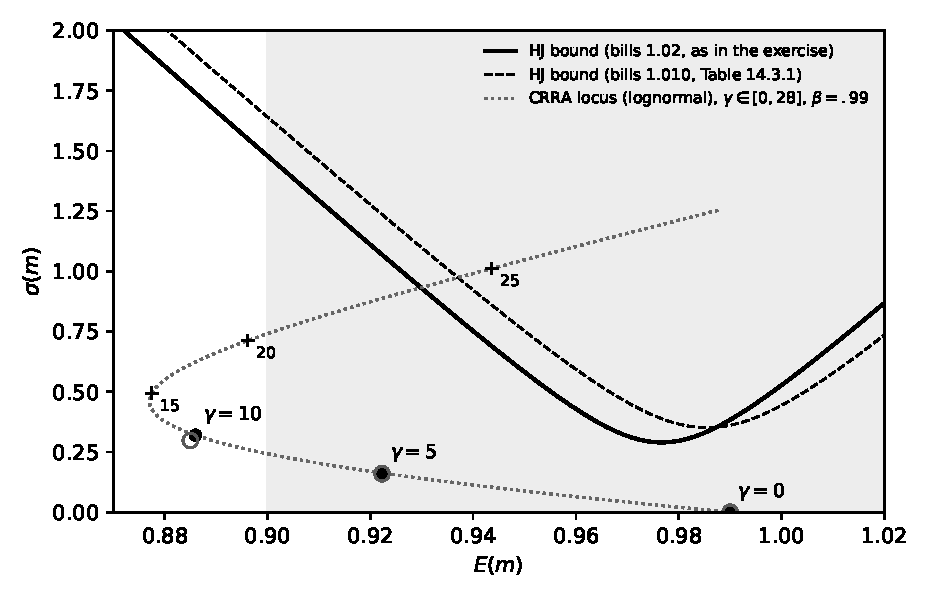
\includegraphics[width=0.78\textwidth]{figures/ch14_01.pdf}\\
{\small Figure S14.1.  Hansen--Jagannathan bounds and CRRA discount factors ($\beta=.99$).  Filled circles: lognormal consumption growth; open circles: two-point
distribution; the dotted line traces the lognormal locus as $\gamma$ rises from 0 to 28 (crosses at $\gamma=15,20,25$).}
\end{center}

\emph{Inference.}  None of the three points is admissible; all lie far below the bound.  With $\gamma=0$ the discount factor is constant.  Raising $\gamma$ raises
$\sigma(m)$, roughly in proportion to $\gamma s_gE(m)$.  But it also lowers $E(m)$, i.e.\ it raises the implied risk-free rate $1/E(m)$ (to 12.9\% at $\gamma=10$), because $\gamma$
also governs intertemporal substitution and consumption grows on average.  The point therefore moves left, into the region where the bound is steep, and the
gap widens: at $\gamma=10$, $\sigma(m)=.32$, while the bound at $E(m)=.886$ is $1.74$.  This is the equity premium puzzle combined with Weil's risk-free rate puzzle
(section \bk{14.6}).  Two calculations make the point sharper.
\begin{itemize}[leftmargin=*]
\item The ratio $\sigma(m)/E(m)=[\exp(\gamma^2s_g^2)-1]^{1/2}$ does not depend on $\beta$.  Admissibility needs it to be at least $.2967$, i.e.\ $\gamma\ge8.30$, and then $\beta$ must
put $E(m)$ at $.977$, which requires $\beta=1.081>1$.  This is Kocherlakota's observation (footnote 15 of the chapter).
\item With $\beta=.99$, $E(m)$ falls until $\gamma=\mu_g/s_g^2=14.1$ (where $E(m)=.877$) and then rises, because the precautionary term $\frac12\gamma^2s_g^2$ takes over.  The
lognormal locus enters the admissible region only at $\gamma=23.8$ ($29.4$ with the two-point distribution).  Section \bk{14.2} explains why such values are
implausible; moreover, at such $\gamma$ the answer depends on the tails of the distribution of consumption growth.
\end{itemize}
With a mean bill return of $1.010$ these thresholds become $\gamma\ge9.87$ with $\beta=1.101$, and $\gamma=24.5$ ($30.3$).
\end{ex}

%%---------------------------------------------------------------------------
\begin{ex}{14.2}{The term structure and regime switching}
Let $k\equiv\gamma\alpha_1>0$ and $\bar r\equiv\rho+\gamma(\alpha_0+\mu)-\frac12\gamma^2\tau^2$.  The discount factor is $m_{t+1}=\beta\exp[-\gamma(\alpha_0-\alpha_1s_t+\varepsilon_{t+1})]$.  Write
$p_s\equiv\Prob(s_{t+1}=1\given s_t=s)$, so $p_0=1-\pi(0)$ and $p_1=\pi(1)$.

\textbf{(a)}  $E_tm_{t+1}=\beta e^{-\gamma(\alpha_0-\alpha_1s_t)}Ee^{-\gamma\varepsilon}=\exp[-\rho-\gamma(\alpha_0-\alpha_1s_t)-\gamma\mu+\frac12\gamma^2\tau^2]$.  So the gross short rate is $R_1(s_t)=e^{r_1(s_t)}$ with
\[
  r_1(s)=\bar r-ks=\rho+\gamma(\alpha_0-\alpha_1s+\mu)-\tfrac12\gamma^2\tau^2 .
\]
It equals $\rho$ plus $\gamma$ times expected log consumption growth, minus a precautionary term.

\textbf{(b)}  The price of one unit at $t+2$ is $q_2(s_t)=E_t[m_{t+1}m_{t+2}]$.  Given $s_t$, $m_{t+1}$ depends only on $\varepsilon_{t+1}$, which is independent of $s_{t+1}$.  So
$q_2(s)=E_t[m_{t+1}]\,E_t[E_{t+1}m_{t+2}]=e^{-r_1(s)}\sum_{s'}\Prob(s'\given s)e^{-r_1(s')}$, and the two-period rate per period, $r_2=-\frac12\log q_2$, is
\[
  r_2(s)=\tfrac12r_1(s)-\tfrac12\log E_s\bigl[e^{-r_1(s')}\bigr]=\bar r-\tfrac12ks-\tfrac12\log\bigl(1-p_s+p_se^k\bigr),\qquad R_2(s)=e^{r_2(s)} .
\]

\textbf{(c)}  \emph{All maturities.}  The same argument gives $q_n(s)=e^{-n\bar r}h_n(s)$ with $h_n(s)=E_s\exp(k\sum_{j=0}^{n-1}s_{t+j})$, so
\[
  r_n(s)=\bar r-\tfrac1n\log h_n(s),\qquad h_1=D\mathbf 1,\quad h_{n+1}=DPh_n,\quad D=\diag(1,e^k),
\]
where $P$ is the transition matrix.  \emph{Claim}: $1\le h_n(0)\le h_n(1)\le e^{nk}$ for all $n$.  The outer inequalities hold because $0\le\sum_js_{t+j}\le n$.  For the middle
one, the ratio $\varrho_n=h_n(1)/h_n(0)$ satisfies $\varrho_1=e^k$ and $\varrho_{n+1}=f(\varrho_n)$ with
\[
  f(\varrho)=e^k\,\frac{1-\pi(1)+\pi(1)\varrho}{\pi(0)+(1-\pi(0))\varrho},\qquad f(1)=e^k .
\]
$f$ is a M\"obius map: increasing if $\pi(0)+\pi(1)>1$, decreasing if $\pi(0)+\pi(1)<1$, and constant ($=e^k$) if $\pi(0)+\pi(1)=1$.  If it is increasing, $\varrho\ge1$ implies $f(\varrho)\ge f(1)=e^k\ge1$.  If it is
decreasing, $f$ maps $[1,e^k]$ into $[f(e^k),e^k]\subset[1,e^k]$, because $f(e^k)\ge1$ (its numerator is at least $e^k$ and its denominator at most $e^k$).  By induction
$\varrho_n\ge1$ for all $n$.  (A grid check in \texttt{ch14.py} over 625 chains, four values of $k$ and 119 maturities finds no violation.)  Consequences:
\begin{itemize}[leftmargin=*]
\item \emph{Levels.}  $r_n(0)-r_n(1)=\frac1n\log\varrho_n\in(0,k)$ for $n\ge2$ (strictly, when $0<\pi(0),\pi(1)<1$): yields of \emph{every} maturity are higher in good times,
but they move less than the short rate.  As $n\to\infty$, $h_n$ becomes proportional to the Perron vector of $DP$, so $\frac1n\log\varrho_n\to0$: the longest yields are
acyclical, $r_\infty=\bar r-\log\lambda_{\max}(DP)$ in both states.
\item \emph{Slope.}  $r_n(0)-r_1(0)=-\frac1n\log h_n(0)\le0$ and $r_n(1)-r_1(1)=k-\frac1n\log h_n(1)\ge0$.  The yield curve is inverted at peaks (rates are expected to fall)
and upward sloping in troughs: the slope is countercyclical.
\item \emph{Term premia.}  By Jensen's inequality, $r_n(s)\le\bar r-\frac knE_s\sum_js_{t+j}=\frac1n\sum_{j<n}E_sr_1(s_{t+j})$: long yields lie below the average expected short rate (a convexity
effect).  There is no \emph{risk} premium, however.  The one-period holding return on any bond depends only on $s_{t+1}$, which is independent of $m_{t+1}$ given $s_t$,
so every bond's expected gross holding return equals $R_1(s_t)$.  The expectations hypothesis holds exactly for gross holding returns.
\end{itemize}

\textbf{(d)}  Procyclical: $r_1(0)-r_1(1)=\gamma\alpha_1>0$.  In good times consumption is expected to grow fast; the rate must be high to dissuade the representative
agent from borrowing against that growth (the inverse of the intertemporal elasticity of substitution is $\gamma$).

\textbf{(e)}  There is a definite answer: by (c), long rates are procyclical too, whatever the parameters, but less so than short rates.  How much less depends on
the permanence of the cycle, which we measure by the autocorrelation $\lambda\equiv\pi(0)+\pi(1)-1$ of $s_t$ (equivalently, the expected durations $1/[1-\pi(s)]$ of the
regimes).  For the two-period rate,
\[
  r_2(0)-r_2(1)=\tfrac12\bigl[k+\log(1-p_1+p_1e^k)-\log(1-p_0+p_0e^k)\bigr],
\]
and $\log(1-p+pe^k)$ increases in $p$.  So the long rate moves by more than half as much as the short rate iff $p_1>p_0$, i.e.\ iff $\lambda>0$.  In the limit of permanent
regimes ($\pi(0),\pi(1)\to1$) it moves one for one with the short rate; with i.i.d.\ regimes ($\lambda=0$) exactly half as much; when the regime alternates every period
($\pi(0),\pi(1)\to0$) not at all.  Long rates average expected future short rates, and only a persistent cycle moves those expectations.  An illustration with
$\beta=.99$, $\gamma=2$, $\alpha_0=.03$, $\alpha_1=.02$, $\mu=.005$, $\tau=.02$ ($k=.04$; $r_1=7.925\%$ and $3.925\%$ in the two states):
\begin{center}
\begin{tabular}{lcccccc}
\toprule
 & \multicolumn{5}{c}{$r_n(0)-r_n(1)$ (percentage points)} & \\
\cmidrule(lr){2-6}
$(\pi(0),\pi(1))$, $\lambda$ & $n=1$ & 2 & 5 & 10 & 40 & $r_\infty$ (\%)\\
\midrule
$(.9,.8)$, $+.7$ & 4 & 3.403 & 2.231 & 1.310 & 0.338 & 6.487\\
$(.6,.4)$, $\phantom{+}0$ & 4 & 2.000 & 0.800 & 0.400 & 0.100 & 6.306\\
$(.3,.2)$, $-.5$ & 4 & 0.998 & 0.550 & 0.266 & 0.067 & 6.052\\
\bottomrule
\end{tabular}
\end{center}
A Monte Carlo evaluation of the two- and five-period bond prices agrees with the formulas to within sampling error (e.g.\ $r_5(1)=5.0773\%$ versus $5.0771\%$).
\end{ex}

%%---------------------------------------------------------------------------
\begin{ex}{14.3}{Growth slowdowns and stock market crashes}
\rmk{The statement writes the growth factor as $\gamma$ in ``$d_{t+1}=\gamma d_t$'' and in ``$d_{T-1}=d_T=\gamma^{(T-1)}$'', but calls it $\nu$ elsewhere, and $\gamma$ is also the
risk-aversion parameter.  The growth factor is $\nu$ throughout.  We also assume that the tree is growing at date 0 ($d_{-1}=1/\nu$).}

\textbf{(a)}  A competitive equilibrium is an ex-dividend share price $p_t$, a function of the history of dividends, and an allocation $\{c_t,s_{t+1}\}$ such that: (i) given
prices, the representative household chooses $\{c_t,s_{t+1}\}$ to maximize $E_0\sum\beta^tu(c_t)$ subject to $c_t+p_ts_{t+1}\le(p_t+d_t)s_t$, $s_0=1$, and a no-Ponzi
condition; (ii) markets clear: $c_t=d_t$ and $s_{t+1}=1$.  The Euler equation and the transversality condition at the equilibrium allocation give
\[
  p_t=E_t\Bigl[\beta\Bigl(\frac{d_{t+1}}{d_t}\Bigr)^{-\gamma}(p_{t+1}+d_{t+1})\Bigr],\qquad\text{so}\qquad p_t=E_t\sum_{j\ge1}\beta^j\Bigl(\frac{d_{t+j}}{d_t}\Bigr)^{-\gamma}d_{t+j}.
\]

\textbf{(b)}  There are two regimes: growing ($G$) and stopped ($S$).  In $S$ the dividend is constant forever, so $p_t=w_Sd_t$ with $w_S=\beta/(1-\beta)$.  In $G$ the
distribution of future growth rates is the same at every date, so $p_t=w_Gd_t$ with a constant price--dividend ratio $w_G$.  Let $x\equiv\nu^{1-\gamma}$.  The Euler equation gives
$w_G=\beta\pi x(1+w_G)+\beta(1-\pi)(1+w_S)$, so
\[
  w_G=\frac{\beta\pi x+\beta(1-\pi)/(1-\beta)}{1-\beta\pi x},\qquad w_G-w_S=\frac{\beta\pi\,(x-1)}{(1-\beta)(1-\beta\pi x)} .
\]
$w_G$ is finite because $\beta\pi x<\beta\nu^{1-\gamma}<1$.  (Summing $\sum_j\beta^jE(d_{t+j}/d_t)^{1-\gamma}$ directly gives the same numbers.)  Hence
\[
  p_t=w_G\,\nu^t\ \ (t<T),\qquad p_t=w_S\,\nu^{T-1}\ \ (t\ge T).
\]
The price is \emph{not} a function of the current dividend alone: at $T-1$ and at $T$ the dividend is the same, $\nu^{T-1}$, but the prices differ unless $\gamma=1$.  It depends
on $(d_t,d_{t-1})$, i.e.\ on the current dividend and on whether it grew last period; that pair is a Markov state.  With $\gamma=1$, $w_G=w_S$ and $p_t=\beta d_t/(1-\beta)$.

\textbf{(c)}  $p_{T-1}-p_T=(w_G-w_S)\nu^{T-1}$, which is positive iff $x>1$, i.e.\ iff $\gamma<1$.  The percentage change at $T$ is
$p_T/p_{T-1}-1=w_S/w_G-1$, with $w_G/w_S-1=\pi(x-1)/(1-\beta\pi x)$.  News that growth has stopped has two effects.  A \emph{cash-flow effect}: future dividends will be
lower, which lowers the price.  A \emph{discount-rate effect}: expected consumption growth falls, so the interest rate falls from
$R^f_G=[\beta(\pi\nu^{-\gamma}+1-\pi)]^{-1}$ to $R^f_S=1/\beta$ and future dividends are discounted less.  With CRRA preferences the intertemporal elasticity of substitution is
$1/\gamma$.  If $\gamma<1$ the cash-flow effect dominates and the market crashes; if $\gamma>1$ the discount-rate effect dominates and the price \emph{jumps up}; with log utility the two
cancel.  An example with $\beta=.96$, $\nu=1.02$, $\pi=.95$ ($w_S=24$, $R^f_S=1.0417$):
\begin{center}
\begin{tabular}{ccccc}
\toprule
$\gamma$ & $w_G$ & $p_T/p_{T-1}-1$ & gross return at $T$ & $R^f_G$\\
\midrule
0.5 & 26.87 & $-10.7\%$ & 0.930 & 1.0515\\
1 & 24.00 & $0$ & 1.042 & 1.0614\\
2 & 19.78 & $+21.3\%$ & 1.264 & 1.0816\\
5 & 12.97 & $+85.0\%$ & 1.927 & 1.1441\\
\bottomrule
\end{tabular}
\end{center}
So in this model a growth slowdown produces a crash only if the intertemporal elasticity of substitution exceeds one.  The crash is then larger the more
surprising the slowdown ($w_G/w_S-1$ increases with $\pi$).  Such crashes are rational responses to news, with no bubble.

\textbf{(d)}  After the switch the market value stops growing: it rose at the rate $\nu$ before and is flat afterwards, at $w_S\nu^{T-1}$.  At the switch itself it jumps by
$w_S/w_G-1$: down if $\gamma<1$, up if $\gamma>1$.  So a pattern of a crash followed by a long stagnation, as in Japan after 1990, is consistent with the model only if the
elasticity of intertemporal substitution exceeds one.  With the conventional $\gamma>1$ the model predicts a boom when growth slows.  To reconcile high risk aversion with
this evidence one needs preferences that separate risk aversion from intertemporal substitution (Epstein--Zin, section \bk{14.7}), as in the long-run risk literature.
\end{ex}

%%---------------------------------------------------------------------------
\begin{ex}{14.4}{The term structure and consumption}
Let $c_t=\log C_t$, $\kappa=\log C^*$ and $e_{t+1}=\log\varepsilon_{t+1}\sim\Norm(-s^2/2,s^2)$ with $s^2=\log(1+\sigma^2)$ (this makes $E\varepsilon=1$, $\var\varepsilon=\sigma^2$).  Then
$c_{t+1}=\kappa+\varphi c_t+e_{t+1}$, a stationary AR(1) with mean $\bar c=(\kappa-s^2/2)/(1-\varphi)$.

\textbf{(a)}  Let $p_t$ be the ex-dividend price of a tree and $Q_{jt}$ the price at $t$ of a claim to one unit of consumption at $t+j$ ($Q_{0t}\equiv1$).  A household holding
$s_t$ trees and $b_{j,t-1}$ bonds bought at $t-1$ with $j$ periods to maturity faces
\[
  c_t+p_ts_{t+1}+\sum_{j\ge1}Q_{jt}b_{jt}\le(p_t+C_t)s_t+\sum_{j\ge1}Q_{j-1,t}\,b_{j,t-1}
\]
(each bond bought as a $j$-period bond is a $(j-1)$-period bond next period), plus a no-Ponzi condition.  A competitive equilibrium is a set of price functions
$p_t,Q_{jt}$ of the state $C_t$ and an allocation such that the allocation solves every household's problem at those prices and markets clear: $c_t=C_t$, $s_{t+1}=1$, and
$b_{jt}=0$ (bonds are in zero net supply).  The Euler equations then give $Q_{jt}=E_t[\beta(C_{t+1}/C_t)^{-\gamma}Q_{j-1,t+1}]=E_t[\beta^j(C_{t+j}/C_t)^{-\gamma}]$.

\textbf{(b)}  From the AR(1), $E_tc_{t+j}-c_t=(1-\varphi^j)(\bar c-c_t)$ and $\var_t(c_{t+j})=s^2(1-\varphi^{2j})/(1-\varphi^2)$.  With the gross yield per period defined by
$Q_{jt}=\tilde R_{jt}^{-j}$,
\[
  \log\tilde R_{jt}=-\frac{\log Q_{jt}}j=\rho+\underbrace{\frac{\gamma(1-\varphi^j)}{j}}_{\equiv b_j}(\bar c-c_t)-\frac{\gamma^2s^2}{2j}\,\frac{1-\varphi^{2j}}{1-\varphi^2} .
\]
For $j=1$: $\log\tilde R_{1t}=\rho+\gamma E_t(c_{t+1}-c_t)-\frac12\gamma^2s^2$.  As $j\to\infty$, $\log\tilde R_{jt}\to\rho$ in every state.  When $C_t$ is above its mean, consumption is expected to
fall, short rates are low and the yield curve rises toward $\rho$; below the mean, short rates are high and the curve falls.  (\texttt{ch14.py} verifies that these prices satisfy
$Q_{j+1,t}=E_t[\beta(C_{t+1}/C_t)^{-\gamma}Q_{j,t+1}]$ by quadrature, to $3\times10^{-16}$.)

\textbf{(c)}  Disagree.  $\var(\log\tilde R_{jt})=b_j^2\var(c_t)=b_j^2s^2/(1-\varphi^2)$, and $b_j=\gamma(1-\varphi)\cdot\frac1j\sum_{i=0}^{j-1}\varphi^i$ is $\gamma(1-\varphi)$ times an average of the first $j$ terms of
the decreasing sequence $\varphi^i$, so it is strictly decreasing in $j$ (e.g.\ with $\gamma=2$, $\varphi=.9$: $b_1=.2$, $b_2=.19$, $b_5=.164$, $b_{10}=.130$, $b_{40}=.049$).  The short rate is the
\emph{most} volatile yield.  Long yields average expected future short rates, and mean reversion makes distant expectations move little.  (Holding a long bond for one
period is riskier than holding a short one, but that is a statement about prices and holding returns, not about the variability of yields.)

\textbf{(d)}  Agree.  $\partial\log\tilde R_{jt}/\partial c_t=-b_j<0$, largest in absolute value at $j=1$ and vanishing as $j\to\infty$.

\textbf{(e)}  Disagree.  The negative relation between rates and consumption is an equilibrium implication of the Euler equation, with causation running from
consumption to rates: a high $C_t$ means consumption is expected to revert, i.e.\ to grow slowly, and a low rate is needed to stop people from wanting to save.  In this
endowment economy consumption is exogenous; nothing the Fed does to interest rates changes it.  Reading a policy lever into an equilibrium correlation is the
error that the Lucas critique warns against.

\textbf{(f)}  Agree, in the limit.  As $\varphi\to1$, $b_j\to0$ for every fixed $j$, and $\log\tilde R_{jt}\to\rho+\gamma(\kappa-s^2/2)-\frac12\gamma^2s^2$ for all $j$: the term structure becomes flat
and constant.  Interest rates depend on expected consumption \emph{growth}, not on its level.  When shocks are permanent (a random walk in $\log C$), a shock moves the
whole expected path of consumption in parallel and leaves expected growth unchanged.
\end{ex}

%%---------------------------------------------------------------------------
\begin{ex}{14.5}{Ambiguity averse multiplier preferences}
\exnote{Equations (1)--(3) refer to the numbered displays of the exercise in the book.}
\textbf{(a)}  Under the guess, $U_{t+1}=k_0+k_1(c_t+\mu)+k_1\sigma_c\varepsilon_{t+1}$ is conditionally normal, so
\[
  -\beta\theta\log E_t\exp(-U_{t+1}/\theta)=\beta\bigl[k_0+k_1(c_t+\mu)\bigr]-\frac{\beta k_1^2\sigma_c^2}{2\theta}.
\]
Matching $k_0+k_1c_t$ with $c_t$ plus this expression: the coefficients on $c_t$ give $k_1=1+\beta k_1$, and the constants give $(1-\beta)k_0=\beta k_1\mu-\beta k_1^2\sigma_c^2/(2\theta)$.  Hence
\[
  k_1=\frac1{1-\beta},\qquad k_0=\frac{\beta}{(1-\beta)^2}\Bigl[\mu-\frac{\sigma_c^2}{2\theta(1-\beta)}\Bigr],
\]
which is \bk{(14.7.9)}.

\textbf{(b)}  $E_tU_{t+1}=k_0+k_1(c_t+\mu)$ and $\var_t(U_{t+1})=k_1^2\sigma_c^2$, so the right side of (3) is $c_t+\beta[k_0+k_1(c_t+\mu)]-\beta k_1^2\sigma_c^2/(2\theta)$, identical to the right side of (1)
computed in (a).  More generally, (1) and (3) coincide whenever $U_{t+1}$ is conditionally Gaussian, by the formula for $\mathsf T_t$ in the preamble.

\emph{The plans.}  Treat the numbers at the nodes as $c_t$ for $t=0,1,2$, with nothing after $t=2$.  In plan A, $c_0=c_1=1$, and at $t=1$ the consumer learns whether
$c_2=2$ or $c_2=0$ (probability $.5$ each).  Plan B has the same payoffs, but nothing is learned at $t=1$, and $c_2\in\{2,0\}$ is revealed at $t=2$.  In plan C, $c_1$ and $c_2$ are
independent draws from $\{2,1\}$; in plan D, $c_1\in\{2,1\}$ and $c_2=c_1$.  All four plans have the same marginal distribution of $c_t$ at each date within each pair, so
with $\theta=\infty$ (expected utility) the consumer is indifferent within each pair.  Applying (3) backward:
\begin{align*}
  U^A_0&=1+\beta+\beta^2-\frac{\beta^3}{2\theta},&
  U^B_0&=1+\beta+\beta^2-\frac{\beta^2}{2\theta},\\
  U^C_0&=1+\tfrac32\beta+\tfrac32\beta^2-\frac{\beta(1+\beta)}{8\theta},&
  U^D_0&=1+\tfrac32\beta+\tfrac32\beta^2-\frac{\beta(1+\beta)^2}{8\theta}.
\end{align*}
(In A, $U_1\in\{1+2\beta,1\}$ has variance $\beta^2$, penalized at $t=0$.  In B, $U_1=1+\beta-\beta/(2\theta)$ in both nodes, because $\var_1(c_2)=1$ is penalized at $t=1$.  In C,
$\var_0(U_1)=\var_1(U_2)=\frac14$; in D, $U_1\in\{2+2\beta,1+\beta\}$ has variance $(1+\beta)^2/4$.)  So
\[
  U^A_0-U^B_0=\frac{\beta^2(1-\beta)}{2\theta}>0,\qquad U^C_0-U^D_0=\frac{\beta^2(1+\beta)}{8\theta}>0 .
\]
\emph{Interpretation.}  Representation (3) charges a penalty, $\beta/(2\theta)$ per unit, on the conditional variance of \emph{continuation utility}.  With early resolution
the risk about $c_2$ enters $U_1$ multiplied by $\beta$; its variance, $\beta^2$, is penalized at $t=0$, for a total of $\beta\cdot\beta^2/(2\theta)$.  With late resolution the same risk is
penalized at $t=1$, where it enters undiscounted, for a total of $\beta\cdot\beta/(2\theta)$.  Because the variance scales with the \emph{square} of the discount factor, resolving risk
early is cheaper.  With persistent risk, one shock moves both $c_1$ and $c_2$, so it moves $U_1$ by $(1+\beta)$ times the shock, and the variance of continuation utility,
$(1+\beta)^2/4$, includes the cross term $2\beta/4$.  With i.i.d.\ risk the two shocks are penalized separately, $(1+\beta)/4$ in total after discounting.  Risk that
accumulates over time is disliked more.  The exact operator (1) applied to these binary lotteries (for which (3) is only a second-order approximation) gives the
same ranking.  For $\beta=.95$, $\theta=1$: $U^A_0=2.476>U^B_0=2.461$ and $U^C_0=3.556>U^D_0=3.385$ (with (3): $2.424$, $2.401$, $3.547$, $3.327$).

\textbf{(c)}  With $U_t=k_0+k_1\log C_t$, $\partial U_t/\partial C_t=k_1/C_t$: this is the effect of raising $C_t$ together with the whole future consumption path, which under the random
walk (2) is proportional to $C_t$.  For the dependence on $C_{t+1}$, let $\varepsilon$ take values $\varepsilon_j$ with probabilities $P_j$, as in appendix \bk{B}, and write $U_{t+1,j}$ for continuation
utility in state $j$.  Then
\[
  \frac{\partial U_t}{\partial C_{t+1,j}}=-\beta\theta\,\frac{P_j\exp(-U_{t+1,j}/\theta)\,(-1/\theta)}{\sum_kP_k\exp(-U_{t+1,k}/\theta)}\,\frac{\partial U_{t+1,j}}{\partial C_{t+1,j}}
  =\beta P_j\,\frac{\exp(-U_{t+1,j}/\theta)}{E_t\exp(-U_{t+1}/\theta)}\,\frac{k_1}{C_{t+1,j}} ,
\]
using $\partial U_{t+1}/\partial C_{t+1}=k_1/C_{t+1}$.  Dividing by the probability $P_j$, i.e.\ expressing the derivative per unit of probability, gives the formula in the exercise.  With a
continuous $\varepsilon$ the same statement reads: a perturbation $\delta C_{t+1}(\varepsilon)$ changes $U_t$ by $E_t[\beta g\,k_1\,\delta C_{t+1}/C_{t+1}]$, where $g=\exp(-U_{t+1}/\theta)/E_t\exp(-U_{t+1}/\theta)$.  The
ratio of the two derivatives is the stochastic discount factor \bk{(14.7.12)}, $m_{t+1}=\beta(C_t/C_{t+1})\,g$; the factor $k_1$ cancels.  (Perturbing only $C_t$, or only $C_{t+1}$,
gives $1/C_t$ and $\beta P_jg_j/C_{t+1,j}$ instead, and the same ratio.)

\textbf{(d)}  By \bk{(14.7.5)}, $(1-\beta)(1-\gamma)=-1/\theta$, so $g=\exp(-U_{t+1}/\theta)/E_t\exp(-U_{t+1}/\theta)$.  Since $U_{t+1}=\text{const}_t+k_1\sigma_c\varepsilon_{t+1}$,
\[
  g(\varepsilon_{t+1})=\frac{\exp(-k_1\sigma_c\varepsilon_{t+1}/\theta)}{\exp(k_1^2\sigma_c^2/(2\theta^2))}=\exp\Bigl(w\varepsilon_{t+1}-\frac{w^2}2\Bigr),\qquad w=-\frac{k_1\sigma_c}\theta=-\frac{\sigma_c}{\theta(1-\beta)} .
\]
Equivalently $w=\sigma_c(1-\gamma)$.  (\texttt{ch14.py} confirms (a), (b) and (d) by Gauss--Hermite quadrature.)
\end{ex}

%%---------------------------------------------------------------------------
\begin{ex}{14.6}{Exponential affine stochastic discount factor}
\exnote{Equation (2) refers to a numbered display of the exercise in the book.}
\textbf{(a)}  Given $z_t$, $\log R_{j,t+1}\sim\Norm(\nu_t-\frac12\alpha_t'\alpha_t,\ \alpha_t'\alpha_t)$, so $E_tR_{j,t+1}=\exp(\nu_t-\frac12\alpha_t'\alpha_t+\frac12\alpha_t'\alpha_t)=e^{\nu_t}$.

\textbf{(b)}  $\log(m_{t+1}R_{j,t+1})=\nu_t-r_t-\frac12\Lambda_t'\Lambda_t-\frac12\alpha_t'\alpha_t+(\alpha_t-\Lambda_t)'\varepsilon_{t+1}$ is conditionally normal, so
\[
  E_t(m_{t+1}R_{j,t+1})=\exp\Bigl(\nu_t-r_t-\tfrac12\Lambda_t'\Lambda_t-\tfrac12\alpha_t'\alpha_t+\tfrac12(\alpha_t-\Lambda_t)'(\alpha_t-\Lambda_t)\Bigr)=\exp(\nu_t-r_t-\alpha_t'\Lambda_t).
\]
Setting this to one gives (2).

\textbf{(c)}  $\nu_t(j)-r_t=\log E_tR_{j,t+1}-\log R^f_t$ is the (log) expected excess return, and (2) says it equals $\sum_i\alpha_{it}(j)\Lambda_{it}$: the exposure of the return to each risk
$\varepsilon_i$ times the price of that risk.  Equivalently $\nu_t-r_t=-\cov_t(\log m_{t+1},\log R_{j,t+1})$.  Only exposure to shocks that move the discount factor earns a premium;
$\Lambda_t$ is the vector of market prices of risk (the maximal Sharpe ratio is approximately $|\Lambda_t|$, by \bk{(14.11.6)}).  Risk premia vary over time if either the prices
($\Lambda_z\ne0$) or the exposures ($\alpha_z\ne0$) depend on the state; they are then quadratic in $z_t$.

\textbf{(d)}  Let log consumption growth be affine in the state with homoskedastic shocks, $c_{t+1}-c_t=\mu_c+\iota'z_t+\sigma_c'\varepsilon_{t+1}$, with $z_t$ following the VAR (for example
$z_t$ may contain $c_t-c_{t-1}$ itself).  Then $\log m_{t+1}=\log\beta-\gamma\mu_c-\gamma\iota'z_t-\gamma\sigma_c'\varepsilon_{t+1}$, which has the required form with
\[
  \Lambda_0=\gamma\sigma_c,\quad \Lambda_z=0,\qquad \delta_1=\gamma\iota,\quad \delta_0=\rho+\gamma\mu_c-\tfrac12\gamma^2\sigma_c'\sigma_c .
\]
The i.i.d.\ case $\iota=0$ is \bk{(14.6.8)}--\bk{(14.6.9)}.  CRRA delivers only \emph{constant} risk prices.  Making $\sigma_c$ depend on $z_t$ would make $\Lambda_t$ affine, but then
$r_t=\rho+\gamma(\mu_c+\iota'z_t)-\frac12\gamma^2|\sigma_c(z_t)|^2$ would be quadratic rather than affine in $z_t$.
\end{ex}

%%---------------------------------------------------------------------------
\begin{ex}{14.7}{Value function for CRRA}
\exnote{Equation (1) refers to a numbered display of the exercise in the book.}
\textbf{(a)}  $C_t^{1-\gamma}=C_0^{1-\gamma}\exp[(1-\gamma)(\mu t+\sigma_c\sum_{s\le t}\varepsilon_s)]$, so $E_0C_t^{1-\gamma}=C_0^{1-\gamma}\exp[t((1-\gamma)\mu+\frac12(1-\gamma)^2\sigma_c^2)]$.  Let
\[
  \kappa\equiv\beta\exp\bigl[(1-\gamma)\mu+\tfrac12(1-\gamma)^2\sigma_c^2\bigr].
\]
The terms of (1) are $\kappa^tC_0^{1-\gamma}/(1-\gamma)$, so
\[
  U_0=\frac{C_0^{1-\gamma}}{(1-\gamma)(1-\kappa)}\qquad\text{if}\qquad \log\beta+(1-\gamma)\mu+\tfrac12(1-\gamma)^2\sigma_c^2<0 .
\]
If $\kappa\ge1$ the sum diverges, to $+\infty$ if $\gamma<1$ and to $-\infty$ if $\gamma>1$.  For $\gamma=0$ the condition is $\beta e^{\mu+\sigma_c^2/2}<1$.  For $\gamma=1$ (utility $\log C$),
$U_0=\sum_t\beta^t(\log C_0+\mu t)=\log C_0/(1-\beta)+\beta\mu/(1-\beta)^2$, finite for every $\mu,\sigma_c$.

\textbf{(b)}  Guess $U_t=AC_t^{1-\gamma}$: $AC_t^{1-\gamma}=C_t^{1-\gamma}/(1-\gamma)+\beta AC_t^{1-\gamma}E_te^{(1-\gamma)(\mu+\sigma_c\varepsilon_{t+1})}$ gives $A=1/[(1-\gamma)(1-\kappa)]$.  The recursion has other solutions:
$U_t+B\beta^{-t}$ satisfies it for any $B$.  Iterating the recursion $T$ times gives $U_0=E_0\sum_{t<T}\beta^tu(C_t)+\beta^TE_0U_T$, so the solution that satisfies (1) is the one with
$\lim_{T\to\infty}\beta^TE_0U_T=0$.  For $U_t=AC_t^{1-\gamma}$ this term is $AC_0^{1-\gamma}\kappa^T\to0$ exactly when $\kappa<1$.  The solutions with $B\ne0$ violate the terminal condition.
\end{ex}

%%---------------------------------------------------------------------------
\begin{ex}{14.8}{Lucas tree economy}
We read the timing as usual: whoever buys the tree at $t$ pays $p_t$ and receives $y_{t+1}+p_{t+1}$ at $t+1$, so $p_t=E_t[m_{t+1}(y_{t+1}+p_{t+1})]$.

\textbf{(a)}  $m_{t+1}=\beta u'(C_{t+1})/u'(C_t)=\beta y_t/y_{t+1}$, which takes the four values $\beta y_s/y_{s'}$.  A one-period risk-free bond pays $1$ in both states, so its price is
$E_tm_{t+1}$ and its gross return is
\[
  R^f(s)=\Bigl[\beta\sum_{s'}P_{ss'}\frac{y_s}{y_{s'}}\Bigr]^{-1},\quad\text{i.e.}\quad
  R^f(L)=\Bigl[\beta\Bigl(\pi_L+(1-\pi_L)\frac{y_L}{y_H}\Bigr)\Bigr]^{-1},
\]
\[
  R^f(H)=\Bigl[\beta\Bigl((1-\pi_H)\frac{y_H}{y_L}+\pi_H\Bigr)\Bigr]^{-1}.
\]

\textbf{(b)}  $p(s)=\beta y_s/(1-\beta)$.  Check: $E_s[\beta\frac{y_s}{y'}(y'+\frac\beta{1-\beta}y')]=\beta y_s(1+\frac\beta{1-\beta})=\frac{\beta y_s}{1-\beta}$.  With log utility the income and substitution effects of dividend news
cancel, and the price--dividend ratio is constant.

\textbf{(c)}  $R_{t+1}=(y_{t+1}+p_{t+1})/p_t=y_{t+1}/(\beta y_t)$: the return is $1/\beta$ times dividend growth.  It takes the values $1/\beta$ (no change), $y_H/(\beta y_L)$ (switch from $L$ to $H$) and
$y_L/(\beta y_H)$ (switch from $H$ to $L$), and it is serially correlated through $s_t$.  Its conditional mean is $E_sR=\beta^{-1}E_s(y'/y_s)$, which exceeds $R^f(s)=[\beta E_s(y_s/y')]^{-1}$ by
Jensen's inequality ($E X\cdot E(1/X)\ge1$).  The equity premium is positive because the return is high exactly when consumption is high.

\textbf{(d)}  A unit of consumption at $\bar t+j$ is worth $E_{\bar t}[\beta^jy_{\bar t}/y_{\bar t+j}]=\beta^jy_s(P^ju^{-1})_s$ at $\bar t$, where $u^{-1}\equiv(1/y_L,1/y_H)'$ and $s=s_{\bar t}$.  Summing over $j\ge1$,
\[
  B(s;\eta)=\eta\,y_s\bigl[(I-\beta P)^{-1}\beta P\,u^{-1}\bigr]_s,\qquad (I-\beta P)^{-1}=\frac1\Delta\begin{bmatrix}1-\beta\pi_H&\beta(1-\pi_L)\\\beta(1-\pi_H)&1-\beta\pi_L\end{bmatrix},
\]
with $\Delta=(1-\beta)[1-\beta(\pi_L+\pi_H-1)]$.  $B$ is proportional to $\eta$.  Although the coupons are certain, the value of the bonds varies with the state, because interest rates do.

\textbf{(e)}  By the same calculation, the claim to $y_t-\eta$ is worth
\[
  E(s;\eta)=\sum_{j\ge1}\beta^jy_s\Bigl[1-\eta(P^ju^{-1})_s\Bigr]=\frac{\beta y_s}{1-\beta}-B(s;\eta).
\]

\textbf{(f)}  $B(s;\eta)+E(s;\eta)=p(s)$ for every $\eta$ and $s$: the Modigliani--Miller theorem.  Pricing is linear, and the bonds and the equity together are exactly the
tree's dividend stream, so how the stream is split does not change its value, and the zero-net-worth entrepreneur just breaks even.  Example ($\beta=.95$, $y_L=1$, $y_H=1.25$,
$\pi_L=.8$, $\pi_H=.9$, $\eta=.5$; closed forms checked against direct solution of $p=M(y+p)$ with $M_{ss'}=\beta P_{ss'}y_s/y_{s'}$):
\begin{center}
\begin{tabular}{lcccccc}
\toprule
state & $R^f$ & $E_sR$ & $p$ & $B$ & $E$ & $B+E$\\
\midrule
$L$ & 1.0965 & 1.1053 & 19.00 & 8.366 & 10.634 & 19.00\\
$H$ & 1.0270 & 1.0316 & 23.75 & 10.209 & 13.541 & 23.75\\
\bottomrule
\end{tabular}
\end{center}
Interest rates are high in the low state, where consumption is expected to rise, so the bonds are worth less there.
\end{ex}

%%---------------------------------------------------------------------------
\begin{ex}{14.9}{Long-run risk, I}
(Here $\rho$ is the persistence of $z_t$, so we write $-\log\beta$ explicitly.)

\textbf{(a)}  $m_{t+1}=\beta\exp[-\gamma(c_{t+1}-c_t)]=\beta\exp[-\gamma(\mu+z_t+\sigma_c\varepsilon_{t+1})]$.

\textbf{(b)}  $E_tm_{t+1}=\beta\exp[-\gamma(\mu+z_t)+\frac12\gamma^2\sigma_c^2]$: the price of a one-period risk-free bond.  The short rate is
\[
  r_t=-\log\beta+\gamma(\mu+z_t)-\tfrac12\gamma^2\sigma_c^2 ,
\]
high when expected consumption growth $\mu+z_t$ is high, and it inherits the persistence of $z_t$.  The price of risk of one-period returns is $\gamma\sigma_c$: the discount factor loads
only on the shock to current consumption.

\textbf{(c)}  $c_{t+2}-c_t=2\mu+(1+\rho)z_t+(\sigma_c+\sigma_z)\varepsilon_{t+1}+\sigma_c\varepsilon_{t+2}$, because $\varepsilon_{t+1}$ moves both $c_{t+1}$ and $z_{t+1}$.  So
\[
  E_t(m_{t+1}m_{t+2})=\beta^2\exp\Bigl(-\gamma\bigl[2\mu+(1+\rho)z_t\bigr]+\tfrac12\gamma^2\bigl[\sigma_c^2+(\sigma_c+\sigma_z)^2\bigr]\Bigr),
\]
the price of a two-period zero-coupon bond.  Its yield per period is
\[
  y_t(2)=-\log\beta+\gamma\mu+\tfrac12\gamma(1+\rho)z_t-\tfrac14\gamma^2\bigl[\sigma_c^2+(\sigma_c+\sigma_z)^2\bigr].
\]
Compared with $r_t$, it responds less to $z_t$ ($\frac12(1+\rho)<1$), and its precautionary term is larger when $\sigma_z>0$, because a shock that lowers consumption today also lowers
expected growth, so two-period consumption growth is riskier than two one-period steps.

\textbf{(d)}  In general, $\sum_{i=1}^n(c_{t+i}-c_{t+i-1})=n\mu+\frac{1-\rho^n}{1-\rho}z_t+\sum_{k=1}^{n}\bigl[\sigma_c+\sigma_z\frac{1-\rho^{n-k}}{1-\rho}\bigr]\varepsilon_{t+k}$, so the $n$-period yield is
\[
  y_t(n)=-\log\beta+\gamma\mu+\gamma\,\frac{1-\rho^n}{n(1-\rho)}\,z_t-\frac{\gamma^2}{2n}\sum_{k=0}^{n-1}\Bigl[\sigma_c+\sigma_z\frac{1-\rho^k}{1-\rho}\Bigr]^2 .
\]
(i) All yields move with $z_t$, with loadings $\gamma(1-\rho^n)/[n(1-\rho)]$ that decline with maturity: short rates are the most volatile.  (ii) The slope $y_t(n)-y_t(1)$ falls when $z_t$ rises:
good news about growth flattens or inverts the curve.  (iii) With $\sigma_z>0$ the average curve slopes \emph{down} toward $-\log\beta+\gamma\mu-\frac12\gamma^2(\sigma_c+\sigma_z/(1-\rho))^2$: long bonds pay off
when growth prospects deteriorate, so they hedge long-run consumption risk and carry negative term premia.  With $\beta=.995$, $\gamma=2$, $\mu=.005$, $\rho=.95$, $\sigma_c=.005$,
$\sigma_z=.0005$ (quarterly), the yields at $z_t=0$ are $1.496$, $1.495$, $1.486$, $1.466$, $1.459\%$ for $n=1,4,20,100,400$ (limit $1.456\%$), and the loadings on $z_t$ are $2$, $1.85$, $1.28$, $0.40$,
$0.10$.  (A Monte Carlo check reproduces $\log E_t(m_{t+1}m_{t+2})$ and $\log E_t(m_{t+1}m_{t+2}m_{t+3})$ to six digits.)

\textbf{(e)}  By the same algebra, $E_0C_t^{1-\gamma}=C_0^{1-\gamma}\exp(a_t+b_tz_0)$, with $b_t=(1-\gamma)\frac{1-\rho^t}{1-\rho}$ and
$a_t=(1-\gamma)\mu t+\frac12(1-\gamma)^2\sum_{k=0}^{t-1}\bigl[\sigma_c+\sigma_z\frac{1-\rho^k}{1-\rho}\bigr]^2$.  So
\[
  U_0=\frac{C_0^{1-\gamma}}{1-\gamma}\sum_{t\ge0}\beta^t\exp(a_t+b_tz_0)\equiv C_0^{1-\gamma}f(z_0).
\]
The summands in $a_t$ converge geometrically to $\sigma_\infty^2\equiv(\sigma_c+\sigma_z/(1-\rho))^2$, and $b_t$ is bounded.  So the terms behave like $\kappa^t$ with
\[
  \kappa=\beta\exp\bigl[(1-\gamma)\mu+\tfrac12(1-\gamma)^2\bigl(\sigma_c+\sigma_z/(1-\rho)\bigr)^2\bigr],
\]
and $U_0$ is finite iff $\kappa<1$.  This is the condition of exercise 14.7 with $\sigma_c$ replaced by the long-run volatility of consumption growth $\sigma_c+\sigma_z/(1-\rho)$.  For
$\gamma=1$, $U_0=\sum_t\beta^tE_0c_t$ is always finite.  \texttt{ch14.py} checks that $f$ satisfies $f(z)=\frac1{1-\gamma}+\beta E[e^{(1-\gamma)(\mu+z+\sigma_c\varepsilon)}f(\rho z+\sigma_z\varepsilon)]$ (the recursion
$U_t=u(C_t)+\beta E_tU_{t+1}$) by quadrature; in the example above $\kappa=.990$.
\end{ex}

%%---------------------------------------------------------------------------
\begin{ex}{14.10}{Long-run risk, II}
\textbf{(a)}  Under the guess,
\[
  U_{t+1}=k_0+k_1(c_t+\mu)+(k_1+\rho k_2)z_t+(k_1\sigma_c+k_2\sigma_z)\varepsilon_{t+1},
\]
so $-\beta\theta\log E_t\exp(-U_{t+1}/\theta)=\beta[k_0+k_1(c_t+\mu)+(k_1+\rho k_2)z_t]-\beta(k_1\sigma_c+k_2\sigma_z)^2/(2\theta)$.  Matching coefficients:
$k_1=1+\beta k_1$, $k_2=\beta(k_1+\rho k_2)$, and $(1-\beta)k_0=\beta k_1\mu-\beta(k_1\sigma_c+k_2\sigma_z)^2/(2\theta)$.  Hence
\[
  k_1=\frac1{1-\beta},\qquad k_2=\frac{\beta}{(1-\beta)(1-\beta\rho)},\qquad k_0=\frac{\beta}{(1-\beta)^2}\Bigl[\mu-\frac{\tilde\sigma^2}{2\theta(1-\beta)}\Bigr],\qquad \tilde\sigma\equiv\sigma_c+\frac{\beta\sigma_z}{1-\beta\rho}.
\]
This is \bk{(14.7.9)} with $\sigma_c$ replaced by $\tilde\sigma$, the response of the present value $(1-\beta)\sum_j\beta^jE_{t+1}c_{t+1+j}$ to the shock $\varepsilon_{t+1}$.  Because $\rho$ is close to one,
$\tilde\sigma$ can be several times $\sigma_c$ even though $\sigma_z$ is small.

\textbf{(b)}  By \bk{(14.7.12)}, $m_{t+1}=\beta e^{-(c_{t+1}-c_t)}g_{t+1}$ with $g_{t+1}=\exp(-U_{t+1}/\theta)/E_t\exp(-U_{t+1}/\theta)=\exp(w\varepsilon_{t+1}-\frac12w^2)$ and
\[
  w=-\frac{k_1\sigma_c+k_2\sigma_z}{\theta}=-\frac{\tilde\sigma}{\theta(1-\beta)}=(1-\gamma)\,\tilde\sigma,\qquad \gamma\equiv1+\frac1{\theta(1-\beta)} .
\]
Thus
\[
  \log m_{t+1}=\log\beta-\mu-z_t-\tfrac12w^2-(\sigma_c-w)\,\varepsilon_{t+1},\qquad r_t=-\log\beta+\mu+z_t-\tfrac12\sigma_c^2+\sigma_cw .
\]
The price of risk is $\sigma_c-w=\gamma\sigma_c+(\gamma-1)\beta\sigma_z/(1-\beta\rho)$.  Unlike the time-separable case of exercise 14.9, where it is $\gamma\sigma_c$, news about long-run growth is
priced, and it is amplified by $1/(1-\beta\rho)$ (the mechanism of Bansal and Yaron).  With $\beta=.995$, $\rho=.95$, $\sigma_c=.005$, $\sigma_z=.0005$ and $\gamma=10$ ($\theta=22.2$):
$\tilde\sigma=.01409$, $w=-.127$, and the price of risk is $.132$, against $\gamma\sigma_c=.050$ without the long-run component.  The worst-case model twists $\varepsilon_{t+1}$ to $\Norm(w,1)$, lowering both
current growth and the persistent component $z_{t+1}$.  (\texttt{ch14.py} verifies the value function and $E_tm_{t+1}=e^{-r_t}$ by quadrature.)
\end{ex}

%%---------------------------------------------------------------------------
\begin{ex}{14.11}{Stochastic volatility}
\textbf{(a)}  The stochastic discount factor is the random variable $m_{t+1}$, measurable with respect to date-$(t+1)$ information, such that the date-$t$ price of any payoff
$x_{t+1}$ is $E_t(m_{t+1}x_{t+1})$.  For this consumer it is the intertemporal marginal rate of substitution $\beta u'(C_{t+1})/u'(C_t)$.

\textbf{(b)}  $m_{t+1}=\beta\exp[-\gamma(\mu+\sigma_c(s_t)\varepsilon_{t+1})]$.

\textbf{(c)}  $E_tm_{t+1}=\beta\exp[-\gamma\mu+\frac12\gamma^2\sigma_c(s_t)^2]$, so $r(s)=-\log\beta+\gamma\mu-\frac12\gamma^2\sigma_c(s)^2$.  The risk-free rate is lower in the high-volatility state: a
precautionary saving motive.  The market price of risk, $[\exp(\gamma^2\sigma_c(s)^2)-1]^{1/2}\approx\gamma\sigma_c(s)$, is higher there.

\textbf{(d)}  Given $s_t$, $\varepsilon_{t+1}$ is independent of $s_{t+1}$, so
\[
  E_t(m_{t+1}m_{t+2})=E_t(m_{t+1})\,E_t\bigl[E_{t+1}m_{t+2}\bigr]=\beta^2e^{-2\gamma\mu+\frac12\gamma^2\sigma_c(s_t)^2}\sum_{s'}P_{s_ts'}\,e^{\frac12\gamma^2\sigma_c(s')^2}.
\]
This is the price of a two-period bond: today's short-bond price times the expected price of a short bond tomorrow.  There is no risk premium (only a convexity term),
because volatility news is uncorrelated with the one-period discount factor.

\textbf{(e)}  For any maturity, $q_n(s)=\beta^ne^{-n\gamma\mu}h_n(s)$ with $h_n=(DP)^{n-1}D\mathbf 1$ and $D=\diag(e^{\gamma^2\sigma_L^2/2},e^{\gamma^2\sigma_H^2/2})$, so $y_n(s)=-\log\beta+\gamma\mu-\frac1n\log h_n(s)$.
Factoring $e^{\gamma^2\sigma_L^2/2}$ out of $D$ gives the structure of exercise 14.2 with $k=\frac12\gamma^2(\sigma_H^2-\sigma_L^2)$.  So yields of \emph{all} maturities are lower in the high-volatility
state, the gap shrinks with maturity, and the yield curve slopes up in the high-volatility state (rates are expected to rise as volatility reverts) and down in the
low-volatility state.  Over time the whole curve shifts when the volatility regime switches, the short end moving most, while very long yields stay put.  With
$\beta=.995$, $\gamma=10$, $\mu=.005$, $\sigma_L=.004$, $\sigma_H=.008$, $\pi_0=.95$, $\pi_1=.9$ (quarterly), the low-minus-high spread is $24.0$, $22.2$, $19.1$, $7.7$ and $1.6$ basis points for $n=1,2,4,20,100$,
and $y_{20}-y_1$ is $-5.5$ basis points in the low- and $+10.8$ in the high-volatility state.  (The levels, about 5.4\% per quarter, reflect the risk-free rate puzzle, $\gamma\mu=.05$;
only the differences matter here.  A Monte Carlo check matches the two-period yields to $3\times10^{-6}$.)

\textbf{(f)}  $s_t$ becomes a hidden state that the consumer must infer.  Let $\hat\pi_t=\Prob(s_t=1\given c^t)$.  After observing $\Delta c_{t+1}$, Bayes' rule and the chain give
\[
  \bar\pi_t=\frac{\hat\pi_t\,\phi_H(\Delta c_{t+1})}{\hat\pi_t\,\phi_H(\Delta c_{t+1})+(1-\hat\pi_t)\,\phi_L(\Delta c_{t+1})},\qquad \hat\pi_{t+1}=\bar\pi_t\pi_1+(1-\bar\pi_t)(1-\pi_0),
\]
where $\phi_s$ is the $\Norm(\mu,\sigma_s^2)$ density; the filter starts from $\hat\pi_0=\tilde\pi_0(1)$.  The discount factor $\beta e^{-\gamma\Delta c_{t+1}}$ is unchanged as a function of $\Delta c_{t+1}$, but
its conditional distribution becomes a mixture of normals.  By the law of iterated expectations, prices are the full-information prices averaged over the posterior:
\[
  E_tm_{t+1}=\beta e^{-\gamma\mu}\Bigl[(1-\hat\pi_t)e^{\frac12\gamma^2\sigma_L^2}+\hat\pi_te^{\frac12\gamma^2\sigma_H^2}\Bigr],
\]
and likewise for $E_t(m_{t+1}m_{t+2})$.  The state becomes the continuous variable $\hat\pi_t\in(0,1)$.  The short rate moves smoothly between the two full-information values, and a
large surprise $|\Delta c_{t+1}-\mu|$ raises $\hat\pi_{t+1}$ and lowers rates.
\end{ex}

%%---------------------------------------------------------------------------
\begin{ex}{14.12}{Unknown \texorpdfstring{$\mu$}{mu}}
\rmk{The printed law of motion contains a term $z_t$ that is never defined in this exercise (it is carried over from the long-run risk exercises), and the
statement mentions $\gamma\ge0$, which plays no role with log utility.  We set $z_t\equiv0$; exercise 14.13 treats the case with $z_t$.  We read the information
assumption as: at date $t$ the consumer has observed $y_s\equiv c_s-c_{s-1}$ for $s=1,\dots,t$.}

\textbf{(a)}  With a normal prior and normal observations $y_s=\mu+\sigma_c\varepsilon_s$, the posterior after $t$ observations is $\mu\sim\Norm(\hat\mu_t,\sigma_t^2)$ with
\[
  \frac1{\sigma_t^2}=\frac1{\sigma_\mu^2}+\frac t{\sigma_c^2},\qquad \hat\mu_t=\sigma_t^2\Bigl(\frac{\hat\mu_0}{\sigma_\mu^2}+\frac{\sum_{s\le t}y_s}{\sigma_c^2}\Bigr),
\]
or recursively $\hat\mu_{t+1}=\hat\mu_t+K_t(y_{t+1}-\hat\mu_t)$ with $K_t=\sigma_t^2/(\sigma_t^2+\sigma_c^2)$.  The predictive distribution is $y_{t+1}\given y^t\sim\Norm(\hat\mu_t,\lambda_t^2)$ with $\lambda_t^2\equiv\sigma_c^2+\sigma_t^2$.  With
log utility the marginal rate of substitution is $\beta C_t/C_{t+1}$ whatever the beliefs, and the beliefs enter through the expectation used for pricing.  Writing
$y_{t+1}=\hat\mu_t+\lambda_t\tilde\varepsilon_{t+1}$, where $\tilde\varepsilon_{t+1}\sim\Norm(0,1)$ is the standardized forecast error (i.i.d.\ from the consumer's point of view),
\[
  m_{t+1}=\beta e^{-y_{t+1}}=\exp\bigl(-r_t-\tfrac12\lambda_t^2-\lambda_t\tilde\varepsilon_{t+1}\bigr),\qquad r_t=-\log\beta+\hat\mu_t-\tfrac12\lambda_t^2 .
\]
This is the form \bk{(14.6.8)} with a time-varying drift and a market price of risk $\lambda_t$ that falls deterministically from $(\sigma_c^2+\sigma_\mu^2)^{1/2}$ to $\sigma_c$.  An econometrician
who knows $\mu$ and imposes rational expectations would instead recover $m_{t+1}$ times the likelihood ratio of the consumer's predictive density to the true one,
$\Norm(y_{t+1};\hat\mu_t,\lambda_t^2)/\Norm(y_{t+1};\mu,\sigma_c^2)$, as in section \bk{14.13} and exercise 14.21.

\textbf{(b)}  $R^f_t=1/E_tm_{t+1}=\beta^{-1}\exp\bigl(\hat\mu_t-\frac12(\sigma_c^2+\sigma_t^2)\bigr)$.  It has two components.
\begin{itemize}[leftmargin=*]
\item $\sigma_t^2\approx\sigma_c^2/t$ falls deterministically, so the precautionary term shrinks and pushes $R^f_t$ up.
\item $\hat\mu_t$ is revised with every observation.  From the consumer's point of view it is a martingale with increments of variance $K_t^2\lambda_t^2=\sigma_t^2-\sigma_{t+1}^2$.
\end{itemize}
Hence, under the consumer's beliefs,
\[
  E_t\log R^f_{t+1}-\log R^f_t=\tfrac12(\sigma_t^2-\sigma_{t+1}^2)>0,\qquad E_tR^f_{t+1}/R^f_t=e^{\sigma_t^2-\sigma_{t+1}^2}>1 :
\]
the risk-free rate is a submartingale and is expected to rise.  But its path is not monotone: bad news about $\mu$ lowers it, and the magnitude of the revisions, governed by
$K_t\approx1/t$, dominates the precautionary drift.  Under the true distribution, $\hat\mu_t\to\mu$ almost surely and $E^P\hat\mu_t$ moves monotonically from $\hat\mu_0$ toward $\mu$, so
$R^f_t\to\beta^{-1}\exp(\mu-\sigma_c^2/2)$; whether it drifts up or down on average depends on whether the prior mean was too low or too high.  With the parameters of exercise
14.13 the precautionary drift is negligible (the shrinking precautionary term raises $\log R^f$ by only $3.1\times10^{-6}$ between $t=0$ and $t=10{,}000$), and the revisions
dominate (Figure S14.2).
\end{ex}

%%---------------------------------------------------------------------------
\begin{ex}{14.13}{Long-run risk, III}
\rmk{The parameter list omits $\sigma_\mu$ and $\sigma_z$.  We choose $\sigma_\mu=.0025$ (prior 95\% interval $[0,.01]$ for mean quarterly growth, i.e.\ 0--4\% a year) and
$\sigma_z=.00005$, the same number as the given $\sigma_{z0}$.  With $\rho=.99$ this $\sigma_z$ makes the long-run component as important for long-run risk as the i.i.d.\ part:
$\sigma_z/(1-\rho)=.005=\sigma_c$.  We simulate data with true values $\mu=.005$ and $z_0=0$.}

\textbf{(a)}  Let $x_t=(\mu,z_t)'$ and $y_{t+1}=c_{t+1}-c_t$.  Then
\[
  x_{t+1}=Ax_t+C\varepsilon_{t+1},\qquad y_{t+1}=Gx_t+D\varepsilon_{t+1},\qquad A=\begin{bmatrix}1&0\\0&\rho\end{bmatrix},\ C=\begin{bmatrix}0\\\sigma_z\end{bmatrix},\ G=\begin{bmatrix}1&1\end{bmatrix},\ D=\sigma_c ,
\]
a state-space system in which the same shock drives the state and the observation.  Let $x_t\given y^t\sim\Norm(\hat x_t,\Sigma_t)$, starting from $\hat x_0=(\hat\mu_0,\hat z_0)'$ and
$\Sigma_0=\diag(\sigma_\mu^2,\sigma_{z0}^2)$.  Conditional on $y^t$, $(x_{t+1},y_{t+1})$ is jointly normal with means $(A\hat x_t,G\hat x_t)$, variances $A\Sigma_tA'+CC'$ and $\Omega_t\equiv G\Sigma_tG'+D^2$, and
covariance $A\Sigma_tG'+CD$.  Conditioning on $y_{t+1}$ gives the Kalman filter with correlated noise:
\[
  K_t=\frac{A\Sigma_tG'+CD}{\Omega_t},\qquad \hat x_{t+1}=A\hat x_t+K_t(y_{t+1}-G\hat x_t),\qquad \Sigma_{t+1}=A\Sigma_tA'+CC'-K_t\Omega_tK_t' .
\]
The predictive distribution of consumption growth is $y_{t+1}\given y^t\sim\Norm(\hat\mu_t+\hat z_t,\Omega_t)$.  As in exercise 14.12, $m_{t+1}=\beta e^{-y_{t+1}}$, and with
$\tilde\varepsilon_{t+1}=(y_{t+1}-G\hat x_t)/\Omega_t^{1/2}$,
\[
  m_{t+1}=\exp\bigl(-r_t-\tfrac12\Omega_t-\Omega_t^{1/2}\tilde\varepsilon_{t+1}\bigr),\qquad r_t=-\log\beta+\hat\mu_t+\hat z_t-\tfrac12\Omega_t,\qquad R^f_t=e^{r_t}.
\]
With full information the rate would be $R^{FI}_t=\beta^{-1}\exp(\mu+z_t-\frac12\sigma_c^2)$.  \emph{Checks}: for $t=30$ the filter reproduces the batch (GLS) conditional mean and
covariance of $x_{30}$, computed directly from the joint normal distribution of $(\mu,z_0,\varepsilon_1,\dots,\varepsilon_{30})$ and $(y_1,\dots,y_{30})$, to $10^{-15}$.  With $\sigma_z=\sigma_{z0}=0$ it
reproduces the conjugate-normal formulas of exercise 14.12 exactly.

\textbf{(b)}  Figure S14.2 shows one simulated path, computed with \texttt{ch14.py} (a Python version of the requested program), together with the exercise 14.12 case (same shocks, $z\equiv0$).
\begin{center}
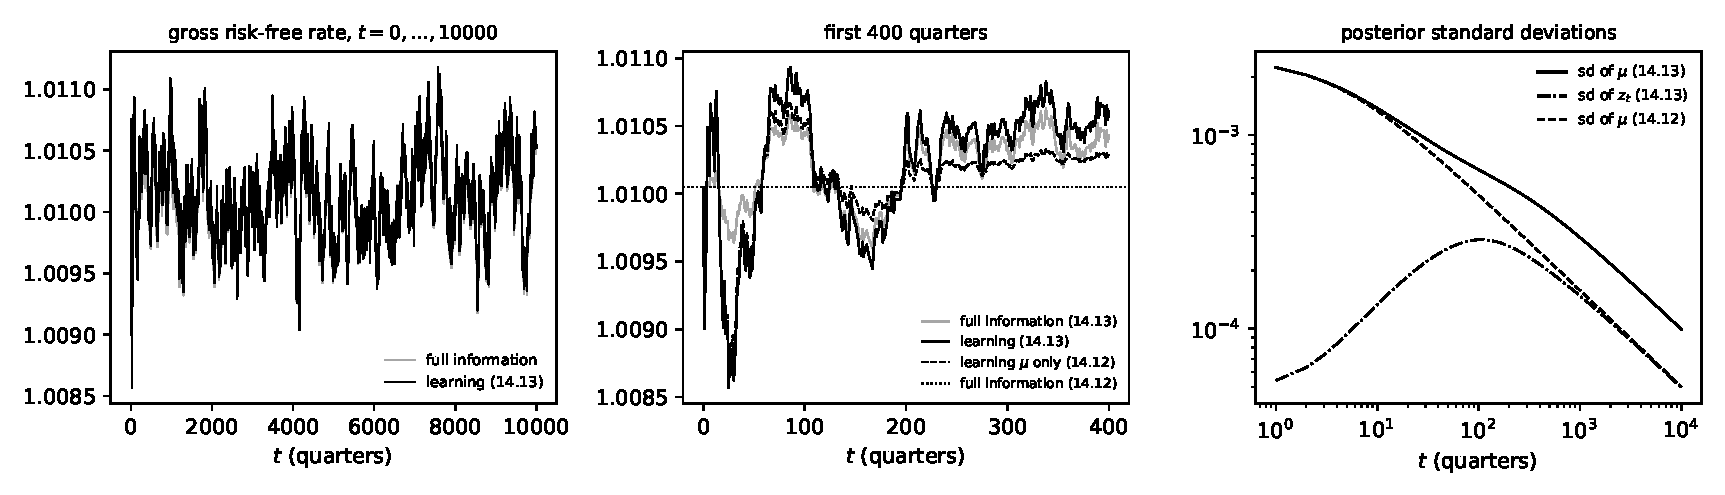
\includegraphics[width=\textwidth]{figures/ch14_13.pdf}\\
{\small Figure S14.2.  Left and middle: gross risk-free rate with learning (black) and with full information (grey), for all 10{,}001 quarters and for the first
400; dashed: learning about $\mu$ only (exercise 14.12).  Right: posterior standard deviations.}
\end{center}
The rate tracks the consumer's estimate of expected growth, $\hat\mu_t+\hat z_t$; the precautionary term is negligible ($\Omega_0-\sigma_c^2=6.25\times10^{-6}$).  Three phases are
visible.
\begin{itemize}[leftmargin=*]
\item \emph{Early learning.}  With few observations, each growth surprise moves $\hat\mu_t$ a lot, so the rate is much more volatile than the full-information rate: its standard
deviation over the first 100 quarters is $6.9\times10^{-4}$, against $2.8\times10^{-4}$.  It starts at $R^f_0=1.01005$ and falls to $1.0090$ after one bad draw.
\item \emph{Slow learning about $\mu$.}  The posterior standard deviation of $\mu$ falls only like $t^{-1/2}$: $6.6\times10^{-4}$ at $t=100$ and $9.9\times10^{-5}$ at $t=10{,}000$.  That is twice
the value when $z$ is absent ($5.0\times10^{-5}$), because a persistent $z_t$ is easily confused with $\mu$: the long-run standard deviation of consumption growth is
$\sigma_c+\sigma_z/(1-\rho)=.01=2\sigma_c$.  The uncertainty about $z_t$ first grows (from $5\times10^{-5}$ to $2.9\times10^{-4}$ near $t=100$), because the unknown $\mu$ contaminates the inference about $z$,
and then falls.
\item \emph{Convergence.}  Because a single shock drives both equations, knowing $\mu$ would reveal $z_t$ exactly:
$z_t=(\rho-\sigma_z/\sigma_c)z_{t-1}+(\sigma_z/\sigma_c)(y_t-\mu)$, and $|\rho-\sigma_z/\sigma_c|=.98<1$.  So $\Sigma_t\to0$ and $R^f_t$ converges to the full-information rate, which fluctuates
persistently with $z_t$ (standard deviation $3.3\times10^{-4}$).  For $t\ge5{,}000$ the two rates differ by at most $5.2\times10^{-5}$.
\end{itemize}
So the risk-free rate is volatile early and becomes a persistent, AR(1)-like process driven by the (eventually learned) long-run growth component.  The precautionary
component of learning contributes only a tiny upward drift.
\end{ex}

%%---------------------------------------------------------------------------
\begin{ex}{14.14}{Affine term structure model}
$p_t(1)=E_tm_{t+1}=\exp(-\delta_0-\delta_1'z_t)$ by \bk{(14.11.5)}, so $\bar A_1=-\delta_0$ and $\bar B_1=-\delta_1$.  (Equivalently, start from $p_t(0)=1$: $\bar A_0=0$, $\bar B_0=0$.)  Suppose
$p_{t+1}(n)=\exp(\bar A_n+\bar B_n'z_{t+1})$.  Then $p_t(n+1)=E_t[m_{t+1}p_{t+1}(n)]$, and
\[
  \log\bigl(m_{t+1}p_{t+1}(n)\bigr)=-\delta_0-\delta_1'z_t-\tfrac12\Lambda_t'\Lambda_t+\bar A_n+\bar B_n'(\mu+\phi z_t)+(C'\bar B_n-\Lambda_t)'\varepsilon_{t+1}
\]
is conditionally normal.  The mean of a lognormal gives
\begin{align*}
  \log p_t(n+1)&=-\delta_0-\delta_1'z_t-\tfrac12\Lambda_t'\Lambda_t+\bar A_n+\bar B_n'(\mu+\phi z_t)+\tfrac12(C'\bar B_n-\Lambda_t)'(C'\bar B_n-\Lambda_t)\\
  &=\bar A_n+\bar B_n'\mu+\tfrac12\bar B_n'CC'\bar B_n-\delta_0+\bigl[\bar B_n'\phi-\delta_1'\bigr]z_t-\bar B_n'C(\Lambda_0+\Lambda_zz_t),
\end{align*}
because the terms $\pm\frac12\Lambda_t'\Lambda_t$ cancel.  Collecting the constant and the coefficient on $z_t$ gives the two recursions: $\bar A_{n+1}=\bar A_n+\bar B_n'(\mu-C\Lambda_0)+\frac12\bar B_n'CC'\bar B_n-\delta_0$ and
$\bar B_{n+1}'=\bar B_n'(\phi-C\Lambda_z)-\delta_1'$.  They are the bond-pricing recursions under the risk-neutral dynamics $z_{t+1}=\mu-C\Lambda_0+(\phi-C\Lambda_z)z_t+C\varepsilon_{t+1}$ of section \bk{14.12}.
\emph{Numerical check} (\texttt{ch14.py}, a two-factor example): the recursion agrees with (i) the closed form $\log E^Q_t\exp(-\sum_{i<n}r_{t+i})$, computed from the Gaussian distribution
of the sum under the risk-neutral dynamics, to $10^{-17}$ for $n\le12$; and (ii) a two-dimensional Gauss--Hermite evaluation of $E_t[m_{t+1}p_{t+1}(n)]$ under the physical
measure, to $5\times10^{-16}$.
\end{ex}

%%---------------------------------------------------------------------------
\begin{ex}{14.15}{Reverse engineering}
\exnote{Equations (0), (1) and (3) refer to the numbered displays of the exercise in the book.}
\textbf{(a)}  $\log(m_{t+1}R_{j,t+1})=-\delta-\mu-\frac12w^2+\eta_{jt}-\frac12(\alpha_j^2+\sigma_j^2)+(w-\sigma_c+\alpha_j)\varepsilon_{t+1}+\sigma_ju_{j,t+1}$, a normal variable with variance $(w-\sigma_c+\alpha_j)^2+\sigma_j^2$.
Setting $E_t(m_{t+1}R_{j,t+1})=1$ and simplifying ($\frac12(w-\sigma_c+\alpha_j)^2-\frac12w^2-\frac12\alpha_j^2=-w\sigma_c+\frac12\sigma_c^2+\alpha_j(w-\sigma_c)$):
\[
  \eta_{jt}=\delta+\mu-\tfrac12\sigma_c^2+w\sigma_c+\alpha_j(\sigma_c-w)=\delta+\mu-\tfrac12\sigma_c^2(2\gamma-1)+\gamma\sigma_c\,\alpha_j .
\]
It does not depend on $t$ or on $\sigma_j$.

\textbf{(b)}  $\eta_{1t}=\delta+\mu-\frac12\sigma_c^2(2\gamma-1)$.  Asset 1 has no exposure to the priced shock $\varepsilon$, and its own risk $u_1$ is independent of $m$, so its expected return
$E_tR_{1,t+1}=e^{\eta_{1t}}$ equals the risk-free rate: $\eta_{1t}=r_t=-\log E_tm_{t+1}$, which is Tallarini's short rate \bk{(14.7.22)} with $\rho=\delta$.

\textbf{(c)}  $\eta_{jt}-\eta_{1t}=\alpha_j(\sigma_c-w)=\alpha_j\gamma\sigma_c$.  The log expected excess return equals the exposure $\alpha_j$ to the shock $\varepsilon$ times its price $\sigma_c-w=\gamma\sigma_c$.  Following
section \bk{14.8.6}, the price splits into $\sigma_c$, the price of consumption risk that a log-utility consumer would charge, and $-w=(\gamma-1)\sigma_c$, a price of model uncertainty.
Exposure to $u_j$ earns nothing: that risk is unpriced even though it raises the variance of the return.

\textbf{(d)}  Take a pure exchange (Lucas tree) economy in which the representative consumer eats the endowment, which follows (0), and ranks consumption plans by
Tallarini's recursion \bk{(14.7.6)},
\[
  U_t=c_t-\beta\theta\log E_t\exp(-U_{t+1}/\theta),\qquad \beta=e^{-\delta},\qquad \theta=\frac{-1}{(1-\beta)(1-\gamma)} .
\]
By \bk{(14.7.12)}--\bk{(14.7.17)} (exercise 14.5), $m_{t+1}=\beta e^{-(c_{t+1}-c_t)}\exp(w\varepsilon_{t+1}-\frac12w^2)$ with $w=-\sigma_c/[\theta(1-\beta)]=\sigma_c(1-\gamma)$, which is (1).  The assets are
claims whose returns satisfy (3), priced by this consumer's Euler equations.

\textbf{(e)}  $\gamma=1$: $w=0$ and $\theta=\infty$.  The recursion becomes $U_t=c_t+\beta E_tU_{t+1}$: time-separable expected log utility, with $m_{t+1}=\beta C_t/C_{t+1}$.

\textbf{(f)}  $\gamma>1$: Epstein--Zin--Weil preferences with a unit elasticity of intertemporal substitution (the aggregator \bk{(14.7.3)} with $\eta=1$) and risk aversion $\gamma$
in the certainty equivalent \bk{(14.7.2)}.  The parameter $\gamma$ governs attitudes toward atemporal risk, and with it the preference for early resolution of uncertainty
(exercise 14.5).  It does not govern intertemporal substitution: that elasticity is fixed at one, which is why $\gamma$ barely affects the risk-free rate in (b).
Alternatively (section \bk{14.8}), the same recursion describes a log-utility consumer who distrusts the model (0) (multiplier preferences).  Then $\theta$, or $\gamma$, measures
the concern about model misspecification, and $\exp(w\varepsilon-\frac12w^2)$ is the likelihood ratio of the worst-case model.
\end{ex}

%%---------------------------------------------------------------------------
\begin{ex}{14.16}{Incomplete markets, I}
\textbf{(a)}  $m^i_{t+1}=\beta(Y^i_{t+1}/Y^i_t)^{-\gamma}=\exp(-\rho-\gamma\mu-\gamma\sigma\epsilon^i_{t+1})$.  They differ unless $\epsilon^1=\epsilon^2$.  With complete markets consumers would trade until their marginal rates
of substitution agreed state by state.  Here only the bond is traded, so only the conditional \emph{means} of the $m^i$, which price the bond, must agree.

\textbf{(b)}  Consumer $i$'s Euler equation for the bond is $1=R_tE_t[\beta(C^i_{t+1}/C^i_t)^{-\gamma}]$.  At $C^i=Y^i$, $E_tm^i_{t+1}=\exp(-\rho-\gamma\mu+\frac12\gamma^2\sigma^2)$, the same for both consumers, so
the Euler equation holds for both iff $r_t=\rho+\gamma\mu-\frac12\gamma^2\sigma^2$.  The Euler equation is also sufficient here.  Let $\{\tilde C_t,\tilde b_{t+1}\}$ be any feasible plan with $\tilde b_0=0$
that satisfies the no-Ponzi condition $\liminf_TE_0\beta^Tu'(C_T)\tilde b_T\ge0$ (no debt left in present value).  By concavity and the budget constraint,
$u(\tilde C_t)-u(C_t)\le u'(C_t)(\tilde C_t-C_t)\le u'(C_t)(\tilde b_t-R_t^{-1}\tilde b_{t+1})$.  Using the Euler equation $\beta^tu'(C_t)R_t^{-1}=\beta^{t+1}E_tu'(C_{t+1})$, the sum telescopes:
\[
  E_0\sum_{t=0}^T\beta^t\bigl[u(\tilde C_t)-u(C_t)\bigr]\le u'(C_0)\tilde b_0-E_0\beta^{T+1}u'(C_{T+1})\tilde b_{T+1},
\]
whose $\limsup$ is $\le0$.  So no trade is optimal for each consumer at this $r_t$, and the bond market clears, $b^1+b^2=0$.  (Lifetime utility is finite if
$\beta\exp[(1-\gamma)\mu+\frac12(1-\gamma)^2\sigma^2]<1$, exercise 14.7.)

\textbf{(c)}  The only traded payoff is a unit that is known at $t$, so every random variable $m_{t+1}$ with $E_tm_{t+1}=e^{-r_t}$ prices all traded assets.  That includes $m^1$, $m^2$, their convex
combinations, and $m^i+e_{t+1}$ for any $e_{t+1}$ with $E_te_{t+1}=0$.  What is unique is the projection of any discount factor on the space of traded payoffs.  Here that is the
constant $E_tm_{t+1}=e^{-r_t}$, the Hansen--Jagannathan $y^*$ of footnote 10.  All discount factors share their conditional mean, i.e.\ the price of the bond.  Different
discount factors would assign different prices to a nontraded risky claim, such as a claim to $Y^1_{t+1}$, and that is the sense in which markets are incomplete.
\end{ex}

%%---------------------------------------------------------------------------
\begin{ex}{14.17}{Incomplete markets, II}
\textbf{(a)}  Given $x_t$, which is known at $t$, $m^i_{t+1}=\exp(-\rho-\gamma(\mu+x_t)-\gamma\sigma\epsilon^i_{t+1})$ (the shock $u_{t+1}$ affects growth only from $t+2$ on).  So
$E_tm^i_{t+1}=\exp(-\rho-\gamma(\mu+x_t)+\frac12\gamma^2\sigma^2)$ for both $i$.  The Euler equations hold at the no-trade allocation iff $r_t=\rho+\gamma(\mu+x_t)-\frac12\gamma^2\sigma^2$.  The
sufficiency argument of exercise 14.16 goes through unchanged with a time-varying $R_t$, and markets clear.

\textbf{(b)}  Expected endowment growth, $\mu+x_t$, is common to both consumers and varies over time.  When it is high, both would like to borrow against their higher
expected future income.  Since bonds are in zero net supply, the interest rate must rise, by $\gamma$ per unit of expected growth (the inverse of the elasticity of intertemporal
substitution), until neither wants to borrow.  In exercise 14.16 expected growth and its variance were constant, and so was the rate.
\end{ex}

%%---------------------------------------------------------------------------
\begin{ex}{14.18}{Incomplete markets, III}
\textbf{(a)}  $\sigma_t$ is known at $t$, so $E_tm^i_{t+1}=\exp(-\rho-\gamma\mu+\frac12\gamma^2\sigma_t^2)$ for both consumers, and the Euler equations hold at no trade iff
\[
  r_t=\rho+\gamma\mu-\tfrac12\gamma^2\sigma_t^2 .
\]
Sufficiency and market clearing follow as in exercise 14.16.

\textbf{(b)}  Rates are low when endowment uncertainty $\sigma_t$ is high: the precautionary motive to save is strong, and the rate must fall until nobody wants to save.  They
are high in calm periods.  Because $\log\sigma_t^2$ is a random walk, $r_t$ has no stationary distribution; it wanders, and can become arbitrarily negative.
\rmk{With $\gamma\ne1$ the lifetime utility $E_0\sum\beta^tu(C_t)$ of the no-trade plan is not finite: already $E_0C_2^{1-\gamma}$ involves
$E\exp[\frac12(1-\gamma)^2\sigma_0^2e^{\sigma_\sigma u_1}]=\infty$, since the exponential of a lognormal variable has no mean.  (Two-period bond prices are infinite for the same
reason, $E_t\exp(\frac12\gamma^2\sigma_{t+1}^2)=\infty$.)  The equilibrium in (a) should therefore be read either with $\gamma=1$, or as the period-by-period Euler-equation
characterization, which involves only one-period-ahead moments and is well defined, or with a volatility process that is bounded above.}
\end{ex}

%%---------------------------------------------------------------------------
\begin{ex}{14.19}{Relative entropy}
\rmk{Minor misprints: $\lambda_t=\lambda_0+\lambda_1'x_t$ should have an $n\times n$ matrix multiplying $x_t$; the twisted mean in (d) is $\mu+\phi x_t-C\lambda_t$ (not $\mu_x$); and in (e)
$\log l_{t+1}=-\frac12\lambda_t'\lambda_t-\lambda_t'\varepsilon_{t+1}$ (a transpose is missing).}

\textbf{(a)}  Assume $C$ is nonsingular and define $\varepsilon_{t+1}=C^{-1}(x_{t+1}-\mu-\phi x_t)$.  Conditional on $x^t$ (the process is Markov), $\varepsilon_{t+1}\sim\Norm(0,C^{-1}CC'C'^{-1})=\Norm(0,I)$.  This
conditional distribution does not depend on $x^t$, so $\varepsilon_{t+1}$ is independent of $x^t$, and hence of $\varepsilon_1,\dots,\varepsilon_t$: the sequence is i.i.d.\ $\Norm(0,I)$, and
$x_{t+1}=\mu+\phi x_t+C\varepsilon_{t+1}$.  (If $CC'$ is singular, apply the construction to its range and complete $\varepsilon$ with independent draws.)

\textbf{(b)}  Given $x_t$, $\lambda_t$ is known and $\log l=-\frac12\lambda_t'\lambda_t-\lambda_t'\varepsilon\sim\Norm(-\frac12\lambda_t'\lambda_t,\lambda_t'\lambda_t)$, so $E_tl=\exp(-\frac12\lambda_t'\lambda_t+\frac12\lambda_t'\lambda_t)=1$.

\textbf{(c)}  $l>0$ and $E_tl=1$.  Explicitly, with $\varphi$ the $\Norm(0,I)$ density,
\[
  \frac{\varphi(\varepsilon+\lambda_t)}{\varphi(\varepsilon)}=\exp\bigl(-\tfrac12(\varepsilon+\lambda_t)'(\varepsilon+\lambda_t)+\tfrac12\varepsilon'\varepsilon\bigr)=\exp\bigl(-\lambda_t'\varepsilon-\tfrac12\lambda_t'\lambda_t\bigr)=l .
\]
So $l_{t+1}$ is the ratio of the $\Norm(-\lambda_t,I)$ density of $\varepsilon_{t+1}$ (numerator: the twisted, e.g.\ risk-neutral, conditional distribution) to its $\Norm(0,I)$ density under the physical
measure (denominator), both conditional on $x_t$.

\textbf{(d)}  Write $\varepsilon=C^{-1}(x-\mu-\phi x_t)$.  The physical density of $x_{t+1}$ is $(2\pi)^{-n/2}|CC'|^{-1/2}\exp(-\frac12\varepsilon'\varepsilon)$.  Multiplying by $l$ gives
$(2\pi)^{-n/2}|CC'|^{-1/2}\exp(-\frac12(\varepsilon+\lambda_t)'(\varepsilon+\lambda_t))$.  Now $\varepsilon+\lambda_t=C^{-1}(x-\tilde m)$ with $\tilde m=\mu+\phi x_t-C\lambda_t$, so
$(\varepsilon+\lambda_t)'(\varepsilon+\lambda_t)=(x-\tilde m)'(CC')^{-1}(x-\tilde m)$: the product is the $\Norm(\mu+\phi x_t-C\lambda_t,CC')$ density.

\textbf{(e)}  By (c), the twisted density of $\varepsilon_{t+1}$ is $\Norm(-\lambda_t,I)$.  Hence
\[
  \operatorname{ent}=E_t(l\log l)=\hat E_t\log l=\hat E_t\bigl[-\tfrac12\lambda_t'\lambda_t-\lambda_t'\varepsilon_{t+1}\bigr]=-\tfrac12\lambda_t'\lambda_t+\lambda_t'\lambda_t=\tfrac12\lambda_t'\lambda_t\ \ge0,
\]
with equality iff $\lambda_t=0$.  A Monte Carlo check with $\lambda=(.3,-.2,.5)'$ gives $E(l\log l)=.1895$ and $\hat E\log l=.1910$, against $\frac12\lambda'\lambda=.19$.
\end{ex}

%%---------------------------------------------------------------------------
\begin{ex}{14.20}{Likelihood ratio process}
\textbf{(a)}  Multiplying the $t$ ratios gives $\xi_t=\xi_0\prod_{s=1}^t\exp(-\lambda'\varepsilon_s-\frac12\lambda'\lambda)=\exp(-\lambda'\sum_{s\le t}\varepsilon_s-\frac t2\lambda'\lambda)$.  Since $\lambda'\sum_s\varepsilon_s\sim\Norm(0,t\lambda'\lambda)$,
$\log\xi_t\sim\Norm(-\frac t2\lambda'\lambda,t\lambda'\lambda)$, and $E\xi_t=\exp(-\frac t2\lambda'\lambda+\frac t2\lambda'\lambda)=1$.

\textbf{(b)}  $\xi_t$ is a function of $\varepsilon^t$, $E|\xi_t|=1<\infty$, and $E[\xi_{t+1}\given\varepsilon^t]=\xi_tE\exp(-\lambda'\varepsilon_{t+1}-\frac12\lambda'\lambda)=\xi_t$.

\textbf{(c)}  With $a=\lambda'\lambda$, $\log\xi_t\sim\Norm(m,s^2)$ with $m=-ta/2$, $s^2=ta$:
\begin{align*}
  &\text{mean }e^{m+s^2/2}=1,\qquad\text{median }e^m=e^{-ta/2},\qquad\text{mode }e^{m-s^2}=e^{-3ta/2},\\
  &\text{variance }(e^{s^2}-1)e^{2m+s^2}=e^{ta}-1,\qquad\text{std }(e^{ta}-1)^{1/2},\qquad\text{skewness }(e^{ta}+2)(e^{ta}-1)^{1/2}.
\end{align*}

\textbf{(d)}  The program (\texttt{lognormal\_cdf} in \texttt{ch14.py}) evaluates $F(x)=\Phi((\log x-m)/s)$ for $x>0$ with the error function.  It agrees with \texttt{scipy.stats.lognorm} to
$10^{-12}$ and with simulated frequencies for $t=1,5$.  With $\lambda=1$ ($a=1$):
\begin{center}
\begin{tabular}{rccccccc}
\toprule
$t$ & $\log_{10}$\,median & $F(0.01)$ & $F(0.5)$ & $F(1)$ & $\log_{10}\Prob(\xi_t>1)$ & $\log_{10}$\,std & $\log_{10}$\,skewness\\
\midrule
1 & $-0.22$ & 0.00002 & 0.4234 & 0.6915 & $-0.51$ & 0.12 & 0.79\\
5 & $-1.09$ & 0.1732 & 0.7905 & 0.8682 & $-0.88$ & 1.08 & 3.26\\
100 & $-21.7$ & 0.999997 & 1.0000 & 0.9999997 & $-6.54$ & 21.7 & 65.1\\
1000 & $-217$ & 1 & 1 & 1 & $-55.9$ & 217 & 651\\
10000 & $-2171$ & 1 & 1 & 1 & $-545$ & 2171 & 6514\\
\bottomrule
\end{tabular}
\end{center}
\begin{center}
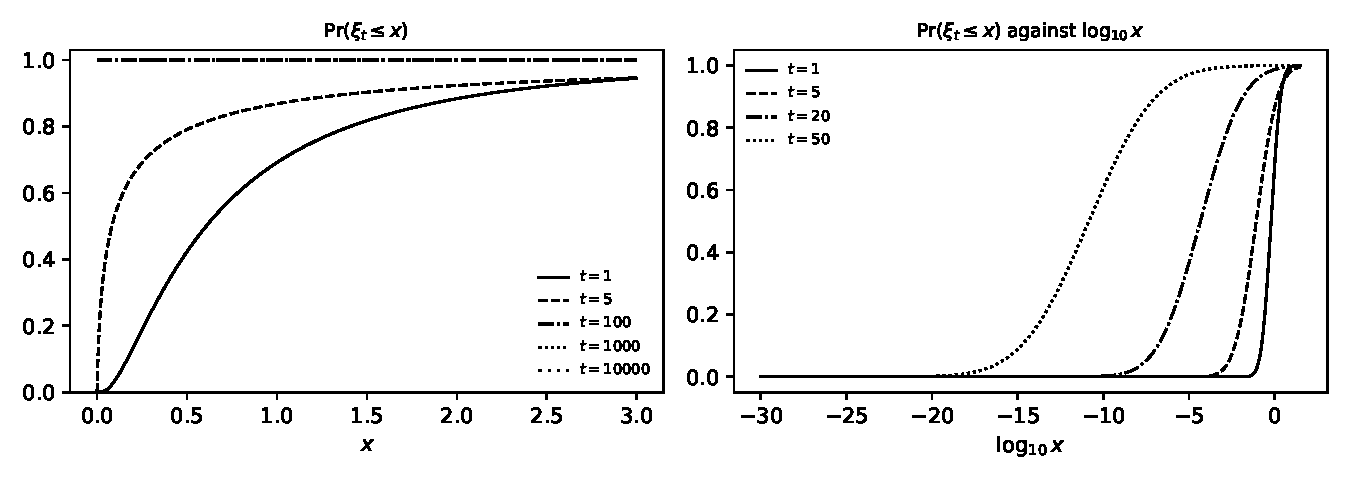
\includegraphics[width=0.9\textwidth]{figures/ch14_20.pdf}\\
{\small Figure S14.3.  C.d.f.\ of $\xi_t$ ($\lambda=1$).  Left: against $x$; for $t\ge100$ it is indistinguishable from $1$ on $(0,3]$.  Right: against $\log_{10}x$, showing the median $e^{-t/2}$ moving left.}
\end{center}
For every $x>0$, $F_t(x)=\Phi\bigl((\log x+t/2)/\sqrt t\bigr)\to1$, so $\xi_t\to0$ in distribution.  In fact $\xi_t\to0$ almost surely, since $\frac1t\log\xi_t\to-\frac12$ by the law of large numbers.  Yet
$E\xi_t=1$ for every $t$.  The mean is carried by events of vanishing probability on which $\xi_t$ is astronomically large: $E[\xi_t\mathbf 1\{\xi_t>1\}]=\Phi(\sqrt t/2)$, which is $.69$, $.87$ and
$1-2.9\times10^{-7}$ for $t=1,5,100$, while $\Prob(\xi_t>1)=\Phi(-\sqrt t/2)$ is $10^{-6.5}$ at $t=100$.  The skewness explodes like $e^{3t/2}$.  The family $\{\xi_t\}$ is not uniformly integrable, so almost-sure
convergence does not carry over to the means: the martingale converges to $\xi_\infty=0$ with $E\xi_\infty=0\ne1$.  Simulation sees only the typical paths: sample means of $10^6$ draws
of $\xi_t$ are $1.00$, $1.00$, $1.01$, $0.15$ and $8\times10^{-6}$ for $t=1,5,20,50,100$.  In the language of section \bk{14.8}, the two probability models become perfectly distinguishable as the
sample grows.  Under the baseline model $\xi_t\to0$, while under the alternative model, for which $\xi_t$ is the likelihood ratio, $\log\xi_t$ has mean $+t/2$ and $\xi_t\to\infty$.
\end{ex}

%%---------------------------------------------------------------------------
\begin{ex}{14.21}{Distorted beliefs}
\rmk{The display defining $m^*_{t+1}$ is unnumbered in the book; we call it (2), as the questions do.  Part (c) refers to the discount factor ``discovered in part a'';
it is found in part (b).}

\textbf{(b)}  (We answer (b) first.)  The subjective density of $\varepsilon$ relative to the physical one is the likelihood ratio $g(\varepsilon)=\varphi(\varepsilon-w)/\varphi(\varepsilon)=\exp(w\varepsilon-\frac12w^2)$, so
$E^S_t(m^*R)=E^P_t(gm^*R)$.  An econometrician who imposes rational expectations therefore recovers
\[
  m_{t+1}=g(\varepsilon_{t+1})\,m^*_{t+1}=\exp\bigl(-\rho-(c_{t+1}-c_t)+w\varepsilon_{t+1}-\tfrac12w^2\bigr)=\exp\bigl(-\rho-\mu-\tfrac12w^2-(\sigma_c-w)\varepsilon_{t+1}\bigr).
\]

\textbf{(a)}  Under the physical measure,
\[
  E(m)=\exp\bigl(-\rho-\mu+\tfrac12\sigma_c^2-\sigma_cw\bigr),\qquad \frac{\sigma(m)}{E(m)}=\bigl[\exp((\sigma_c-w)^2)-1\bigr]^{1/2}\approx\sigma_c-w .
\]
The belief distortion $w$ sets the market price of risk: pessimism ($w<0$) makes it large even though $\sigma_c$ is small.  It also raises $E(m)$ through $-\sigma_cw$ (a pessimist
expects low growth and wants to save, which lowers the risk-free rate), which helps with the risk-free rate puzzle as well.  The discount rate $\rho$ moves $E(m)$
without affecting the market price of risk.  Together, $(w,\rho)$ can place $(E(m),\sigma(m))$ anywhere above the bound.  With the annual data of exercise 14.1 (bills $1.02$), the
point of the bound with the smallest market price of risk ($.2967$ at $E(m)=.977$) is attained with $w=-.2555$ and $\rho=.0156$ ($\beta=.9845$), a perfectly ordinary discount factor.  The
implied distortion of mean log growth, $\sigma_cw=-.0089$, is a quarter of a standard deviation of annual growth.  Its entropy is $w^2/2=.033$ per year, and with 90 annual
observations the detection error probability (section \bk{14.8.7}) is $\Phi(-\sqrt{90}\,|w|/2)=.113$ (simulated: $.112$): a distortion that is hard to detect statistically.

\textbf{(c)}  This $m_{t+1}$ is exactly Tallarini's \bk{(14.7.17)}, with $\beta=e^{-\rho}$ and $w=\sigma_c(1-\gamma)$, i.e.\ risk aversion $\gamma=1-w/\sigma_c$ ($8.30$ in the example; $\gamma>1$ corresponds to
$w<0$), or $\theta=-\sigma_c/[w(1-\beta)]$.  So a log-utility agent with pessimistic beliefs, Tallarini's risk-sensitive agent (unit elasticity of substitution, risk aversion $\gamma$), and the
ambiguity-averse agent of section \bk{14.8} whose worst-case model has mean shift $w$ (equation \bk{(14.8.11)}) are observationally equivalent for asset prices.  The difference is
the source of $w$.  For Tallarini, and under robustness, $w=-\sigma_c/[\theta(1-\beta)]$ is endogenous: it moves with the volatility of consumption.  With distorted beliefs, $w$ is a
primitive.
\end{ex}

%%---------------------------------------------------------------------------
\begin{ex}{14.22}{Costs of aggregate fluctuations}
\exnote{Equations (2) and (3) refer to the numbered displays of the exercise in the book.}
\rmk{In (g) the value should satisfy recursion (3), not (2).}

\textbf{(a)}  $C_{t+j}=C_t\exp(j\mu+\sigma_c\sum_{i=1}^j\varepsilon_{t+i})$, and $\log(C_{t+j}/C_t)\sim\Norm(j\mu,j\sigma_c^2)$, so
\[
  E^P_tC_{t+j}=C_t\,e^{j(\mu+\sigma_c^2/2)},\qquad \operatorname{std}^P_tC_{t+j}=C_t\,e^{j(\mu+\sigma_c^2/2)}\bigl(e^{j\sigma_c^2}-1\bigr)^{1/2}.
\]

\textbf{(b)}  Guess $U^P_t=a+bc_t$: $a+bc_t=c_t+\beta(a+b(c_t+\mu))$ gives $b=1/(1-\beta)$ and $a=\beta\mu/(1-\beta)^2$.  So $U^P_t=\dfrac{c_t}{1-\beta}+\dfrac{\beta\mu}{(1-\beta)^2}$, with state $c_t=\log C_t$.

\textbf{(c)}  Under $S$, $E^S_t(c_{t+1}-c_t)=\mu+\sigma_cw$, so $U^S_t=\dfrac{c_t}{1-\beta}+\dfrac{\beta(\mu+\sigma_cw)}{(1-\beta)^2}$.

\textbf{(d)}  $e^{g^P}=E^P(C_{t+1}/C_t)=e^{\mu+\sigma_c^2/2}$, so $g^P=\mu+\frac12\sigma_c^2$.  It rises one for one with $\mu$ and increases with $\sigma_c$: for a given mean of log growth, more volatility raises
the mean of the level (Jensen).

\textbf{(e)}  $g^S=\mu+\sigma_cw+\frac12\sigma_c^2$.  It rises with $\mu$ and with $w$ ($\partial g^S/\partial w=\sigma_c$); $\partial g^S/\partial\sigma_c=w+\sigma_c$, so more volatility \emph{lowers} subjective mean growth when the
agent is pessimistic enough, $w<-\sigma_c$.

\textbf{(f)}  A deterministic path has the same value for both types: $U^d_0=\log\tilde C_0/(1-\beta)+\beta g/(1-\beta)^2$.  Equating this, with $g=g^P$, to $U^P_0$ gives
\[
  \log\tilde C^P_0=\log C_0+\frac{\beta(\mu-g^P)}{1-\beta}=\log C_0-\frac{\beta\sigma_c^2}{2(1-\beta)},\qquad \tilde C^P_0=C_0\exp\Bigl(-\frac{\beta\sigma_c^2}{2(1-\beta)}\Bigr),
\]
formula \bk{(14.9.3)} with $\gamma=1$.

\textbf{(g)}  Likewise, $\log\tilde C^S_0=\log C_0+\beta(\mu+\sigma_cw-g^S)/(1-\beta)=\log C_0-\beta\sigma_c^2/[2(1-\beta)]$: the same answer.  Each type compares the risky path with a certain path having the growth
rate \emph{it} expects, so the distortion $w$ cancels.  Both types bear the same cost of \emph{risk}.

\textbf{(h)}  The type-$S$ consumer is indifferent between being type $S$ with $C_0$ and type $P$ with $C_0e^{-\Delta}$, where $U^P_0(C_0e^{-\Delta})=U^S_0(C_0)$, i.e.
\[
  \Delta=-\frac{\beta\sigma_cw}{1-\beta}\qquad(>0\text{ for }w<0).
\]
Interpretation: type $P$ faces risk only, with a trusted model.  Type $S$ evaluates the same risk under a pessimistic distortion: this is how the ambiguity-averse (multiplier)
consumer of section \bk{14.8} evaluates plans, with $w=-\sigma_c/[\theta(1-\beta)]$ the worst-case mean shift.  So $\Delta$ measures the cost of \emph{model uncertainty}, on top of the common cost of
risk from (f)--(g).  Two qualifications.  First, the multiplier consumer's value adds back the entropy penalty, $\theta$ times discounted entropy $w^2/2$, which halves the cost:
$\Delta_{\text{mult}}=-\beta\sigma_cw/[2(1-\beta)]$, and then risk plus model uncertainty add up to $\beta\gamma\sigma_c^2/[2(1-\beta)]$, Tallarini's \bk{(14.9.3)} with $\gamma=1-w/\sigma_c$.  Second, the magnitudes differ
enormously.  With the quarterly estimates of Table \bk{14.6.1} ($\mu=.004952$, $\sigma_c=.00505$), $\beta=.995$ and $w=(1-50)\sigma_c=-.2475$ (Tallarini's $\gamma=50$), and measuring costs in
logs of initial consumption as in \bk{(14.9.3)}: the cost of risk is $0.25\%$ of consumption; the payment $\Delta$ is $24.9\%$; with the entropy penalty it is $12.4\%$, and risk plus model uncertainty total $12.7\%$, equal to \bk{(14.9.3)} with $\gamma=50$.  This is the
message of Figure \bk{14.9.1}: the cost of risk is small, while the cost of model uncertainty can be large.
\end{ex}

%%---------------------------------------------------------------------------
\begin{ex}{14.23}{Reverse engineering}
\exnote{Equation (1) refers to a numbered display of the exercise in the book.}
\rmk{As printed, (1) cannot be a pricing kernel: the quadratic term enters with a $+$ sign, so the integral diverges.  It should be $-(x_{t+1}-x_t-\mu)^2/(2\sigma_x^2)$.  Moreover,
the normal density written there is a density for $x_{t+1}$, so the price of $\{X_{t+1}\in\mathcal A\}$ is $\int_{\log\mathcal A}Q\,dx_{t+1}$, or $\int_{\mathcal A}Q\,X_{t+1}^{-1}dX_{t+1}$.  We use the corrected kernel
$Q=e^{-\rho-\gamma(x_{t+1}-x_t)}f(x_{t+1}\given x_t)$ with $f$ the $\Norm(x_t+\mu,\sigma_x^2)$ density of $x_{t+1}$.}

\textbf{(a)}  A Lucas tree economy.  One perishable good, no production (the only technology is the tree), and an endowment $C_t=X_t$ with
$x_{t+1}=x_t+\mu+\sigma_x\varepsilon_{t+1}$, $\varepsilon$ i.i.d.\ $\Norm(0,1)$ under the true probabilities.  A representative consumer has preferences $E_0\sum_t\beta^tC_t^{1-\gamma}/(1-\gamma)$ with $\beta=e^{-\rho}$.  In a
competitive equilibrium with complete Arrow markets, consumption equals the endowment, and the price of the Arrow security paying in state $x_{t+1}$ is
$\beta u'(C_{t+1})/u'(C_t)$ times its probability: $e^{-\rho}e^{-\gamma(x_{t+1}-x_t)}f(x_{t+1}\given x_t)=Q$.  The same kernel arises with any number of consumers having these identical CRRA preferences:
with complete markets they consume constant shares of $X_t$, and their common marginal rate of substitution is the one above.

\textbf{(b)}  With complete markets a representative agent always exists in the sense of chapter 8: Arrow prices equal the marginal rate of substitution of a planner
with Negishi weights, whose utility is CRRA with the same $\gamma$ when individual utilities are identical CRRA.  But $Q$ identifies only the product ``discount factor $\times$
marginal rate of substitution $\times$ probability,'' not its three factors.  For example,
\[
  e^{-\gamma\Delta x}\,\Norm(\Delta x;\mu,\sigma_x^2)=e^{-(\gamma-1)\mu+\frac12(\gamma-1)^2\sigma_x^2}\,e^{-\Delta x}\,\Norm\bigl(\Delta x;\mu-(\gamma-1)\sigma_x^2,\sigma_x^2\bigr),
\]
so the same Arrow prices are generated by a log-utility agent with discount rate $\rho+(\gamma-1)\mu-\frac12(\gamma-1)^2\sigma_x^2$ and pessimistic beliefs.  They are also generated by
Tallarini's agent with risk aversion $\gamma$ and unit elasticity of substitution (exercise 14.21 with $w=\sigma_x(1-\gamma)$).  The representative agent is not unique.

\textbf{(c)}  $\int Q\,dx_{t+1}=e^{-\rho}E\,e^{-\gamma\Delta x}=\exp(-\rho-\gamma\mu+\frac12\gamma^2\sigma_x^2)$, so the one-period risk-free yield is $r=\rho+\gamma\mu-\frac12\gamma^2\sigma_x^2$, as in \bk{(14.6.9)}.

\textbf{(d)}  With the physical measure $x_{t+1}-x_t\sim\Norm(\mu,\sigma_x^2)$, the discount factor is $m_{t+1}=Q/f=\exp(-\rho-\gamma(x_{t+1}-x_t))$.  \emph{Given} the physical measure it is unique
(almost surely): markets are complete, so the Arrow securities span all payoffs, and any $m$ that prices them must equal $Q/f$ state by state.  But $Q$ alone does not reveal the
physical measure.  Any density $\tilde f$ with the same support yields a discount factor $\tilde m=Q/\tilde f$ that prices everything.  An extreme case is the risk-neutral measure
$\tilde f=Qe^{r}$, i.e.\ $x_{t+1}-x_t\sim\Norm(\mu-\gamma\sigma_x^2,\sigma_x^2)$, with the constant discount factor $\tilde m=e^{-r}$.

\textbf{(e)}  $\log m_{t+1}\sim\Norm(-\rho-\gamma\mu,\gamma^2\sigma_x^2)$, so the market price of risk is
\[
  \frac{\sigma(m)}{E(m)}=\bigl[\exp(\gamma^2\sigma_x^2)-1\bigr]^{1/2}\approx\gamma\sigma_x .
\]
If $X_t$ is aggregate consumption, $\sigma_x$ is about $.005$ per quarter or $.035$ per year.  The market price of risk is then $.051$ quarterly and $.36$ annually for $\gamma=10$, and
$.26$ quarterly for $\gamma=50$.  With the annual bound of exercise 14.1, which requires at least $.297$, one needs $\gamma\ge8.3$, and then a $\beta>1$ ($\rho<0$) to put $E(m)$ where the bound is lowest.  So
the model does not attain the bounds with reasonable parameters: it has the equity premium and risk-free rate puzzles of section \bk{14.6}.  It could do so only if $X$ were
a state far more volatile than consumption, which would contradict the reverse engineering of (a).
\end{ex}

%%---------------------------------------------------------------------------
\begin{ex}{14.24}{Unpriced risk}
\rmk{The book writes $\eta_t(j)=\eta_0(j)+\alpha_z(j)z_t$ (the matrix should be $\eta_z(j)$, as the next sentence says) and $\eta_t(j)'u_{t+j}$ (the shock is $u_{t+1}$); the
pricing condition in (b) is the conditional one, $E_t$.}

\textbf{(a)}  Given $z_t$, $\log R_{j,t+1}$ is normal with mean $\nu_t-\frac12\alpha_t'\alpha_t-\frac12\eta_t'\eta_t$ and variance $\alpha_t'\alpha_t+\eta_t'\eta_t$ ($\varepsilon$ and $u$ are independent), so $E_tR_{j,t+1}=e^{\nu_t}$.

\textbf{(b)}  $\log(m_{t+1}R_{j,t+1})=\nu_t-r_t-\frac12\lambda_t'\lambda_t-\frac12\alpha_t'\alpha_t-\frac12\eta_t'\eta_t+(\alpha_t-\lambda_t)'\varepsilon_{t+1}+\eta_t'u_{t+1}$, with conditional variance $(\alpha_t-\lambda_t)'(\alpha_t-\lambda_t)+\eta_t'\eta_t$.  So
$E_t(m_{t+1}R_{j,t+1})=\exp(\nu_t-r_t-\alpha_t'\lambda_t)$, and
\[
  \nu_t(j)=r_t+\alpha_t(j)'\lambda_t=\delta_0+\delta_1'z_t+\bigl(\alpha_0(j)+\alpha_z(j)z_t\bigr)'\bigl(\lambda_0+\lambda_zz_t\bigr),
\]
a quadratic function of $z_t$ that does not involve $\eta_t(j)$.

\textbf{(c)}  The shocks $\varepsilon$ move the discount factor, with loadings $-\lambda_t$.  An asset with exposure $\alpha_t(j)$ pays off badly when $m$ is high (marginal utility is high) to the
extent that $\alpha_t(j)'\lambda_t>0$, so it must offer a higher expected return: $\alpha_t(j)'\lambda_t=\sum_i(\text{exposure to }\varepsilon_i)\times(\text{price of }\varepsilon_i)$, as in exercise 14.6.

\textbf{(d)}  It does not depend on $\eta_t(j)$ at all.  The risk $u_{t+1}$ is independent of the discount factor, so it is not priced: bearing it earns no compensation, however large
it is.  It is diversifiable, idiosyncratic risk from the point of view of the pricing kernel.  The $-\frac12\eta_t'\eta_t$ term in the return is only a convexity adjustment that keeps $E_tR$
equal to $e^{\nu_t}$; it lowers the expected \emph{log} return by $\frac12\eta_t'\eta_t$ but leaves the expected gross return unchanged.  Under the risk-neutral measure of section
\bk{14.12}, $u$ keeps its physical distribution while the mean of $\varepsilon$ shifts to $-\lambda_t$.
\end{ex}

%% ===========================================================================
%% Chapter 15. Economic Growth
%% ===========================================================================
\solchapter{15}{Economic Growth}

\begin{center}
\begin{minipage}{0.86\textwidth}
\small
Solutions to all 6 exercises of Chapter 15 of Ljungqvist and Sargent, \emph{Recursive Macroeconomic Theory} (4th edition, 2018), all
donated by Rodolfo Manuelli.  The numerical illustration in exercise 15.3 comes from \texttt{code/ch15.py}.
\end{minipage}
\end{center}

\bigskip
\hrule
\bigskip

Notation: $\rho\equiv1/\beta-1$ is the rate of time preference, so the modified golden rule is ``net marginal product $=\rho$.''

%%---------------------------------------------------------------------------
\begin{ex}{15.1}{Productive government spending}
\textbf{(a)}  Substituting the constraints, $c_t=f(k_t,g_t)+(1-\delta)k_t-k_{t+1}-g_t$.  The first-order conditions for $g_t$ and $k_{t+1}$ are
\[
  f_g(k_t,g_t)=1,\qquad u'(c_t)=\beta u'(c_{t+1})\bigl[f_k(k_{t+1},g_{t+1})+1-\delta\bigr],
\]
together with the resource constraint and the transversality condition $\lim_t\beta^tu'(c_t)k_{t+1}=0$.  Government spending is a static input: it is set each period
where its marginal product equals its unit cost.

\textbf{(b)}  In a steady state, $f_g(k,g)=1$ and $f_k(k,g)=\rho+\delta$.  Let $g(k)$ solve $f_g(k,g)=1$.  It is unique because $f_{gg}<0$, and it exists if $f_g(k,0^+)>1>\lim_{g\to\infty}f_g$.  Define
$\phi(k)=f_k(k,g(k))$.  Since $g'(k)=-f_{gk}/f_{gg}$,
\[
  \phi'(k)=f_{kk}-\frac{f_{kg}^2}{f_{gg}}=\frac{f_{kk}f_{gg}-f_{kg}^2}{f_{gg}}<0 ,
\]
by strict concavity (a positive Hessian determinant and $f_{gg}<0$).  Under the assumption $\lim_{k\to0}\phi(k)>\rho+\delta>\lim_{k\to\infty}\phi(k)$, there is a unique steady state $k^*$
with $\phi(k^*)=\rho+\delta$, and $g^*=g(k^*)$.

\textbf{(c)}  A higher $\beta$ lowers $\rho+\delta$, and since $\phi$ is decreasing, $k^*$ rises.  Then $dg^*/d\beta=g'(k^*)\,dk^*/d\beta$ has the sign of $f_{gk}$: government spending rises with
patience if $g$ and $k$ are complements ($f_{gk}>0$, as with Cobb--Douglas) and falls if they are substitutes.

\textbf{(d)}  With $f=zk^\alpha g^\eta$ and $y=f$: $f_g=\eta y/g=1$ gives $g/y=\eta$, and $f_k=\alpha y/k=\rho+\delta$ gives $k/y=\alpha/(\rho+\delta)$, so investment is
$x/y=\delta k/y=\alpha\delta/(\rho+\delta)$.  \emph{Both ratios are independent of $z$}: technology changes the scale of the economy but not the steady-state shares, because the
optimality conditions pin down \emph{shares} of output under Cobb--Douglas technology.  The levels scale up:
$y=z^{1/(1-\alpha-\eta)}\bigl[(\alpha/(\rho+\delta))^\alpha\eta^\eta\bigr]^{1/(1-\alpha-\eta)}$.
\end{ex}

%%---------------------------------------------------------------------------
\begin{ex}{15.2}{Productivity and employment}
\textbf{(a)}  Steady-state conditions:
\[
  zf_k(k,n)=\rho+\delta,\qquad \frac{u_2(c,1-n)}{u_1(c,1-n)}=zf_n(k,n),\qquad c=zf(k,n)-\delta k-g .
\]
\emph{Assumptions:} $f$ is homogeneous of degree one, so the first equation pins down $\kappa\equiv k/n$ uniquely (using $f_{kk}<0$ and Inada conditions).  The wage
$w=zf_n(\kappa,1)$ and output net of depreciation per worker, $a=zf(\kappa,1)-\delta\kappa>0$, are then constants, and $c(n)=an-g$.  Uniqueness of $n$ follows if both consumption
and leisure are normal goods.  Then the marginal rate of substitution $u_2/u_1$ along $c=an-g$ is increasing in $n$: more consumption and less leisure both raise the value of leisure.
Existence requires $u_2/u_1<w$ at the lowest feasible $n$ ($c=0^+$) and $u_2/u_1\to\infty$ as $n\to1$ (Inada in leisure).  Interpretation: normality means extra wealth is
spent partly on leisure, so the labor-supply curve crosses the fixed wage only once.

\textbf{(b)}  Here $u_2/u_1=\frac{1-\mu}{\mu}\frac c{1-n}$, $\kappa=\bigl(z\alpha/(\rho+\delta)\bigr)^{1/(1-\alpha)}$, $w=z(1-\alpha)\kappa^\alpha$ and $a=z\kappa^\alpha[1-\alpha\delta/(\rho+\delta)]$.  Both $w$ and $a$ are
proportional to $z^{1/(1-\alpha)}$.  The labor condition $\frac{1-\mu}{\mu}(an-g)=w(1-n)$ gives
\[
  n=\frac{w+\frac{1-\mu}{\mu}g}{w+\frac{1-\mu}{\mu}a}=\frac{1+\frac{1-\mu}{\mu}\frac gw}{1+\frac{1-\mu}{\mu}\frac aw}.
\]
$a/w=[1-\alpha\delta/(\rho+\delta)]/(1-\alpha)$ does not depend on $z$.  So, if $g=0$, employment is \emph{independent of productivity}: income and substitution effects cancel under
these balanced-growth preferences.  With $g>0$ fixed, a higher $z$ lowers $g/w$ and hence \emph{reduces} $n$: the government's claim becomes relatively smaller, a positive wealth
effect.  Output per capita $y=z\kappa^\alpha n\propto z^{1/(1-\alpha)}n$ rises with $z$ in either case, one for one in the $z^{1/(1-\alpha)}$ scale when $g=0$.  ($\sigma$ plays no role in the
steady state.)

\textbf{(c)}  With constant returns, $k/n=\kappa$ is pinned down by $zf_k(\kappa,1)=\rho+\delta$ and is \emph{independent of} $g$.  So an increase in $g$ can raise $k/n$ only if $f$ is not
constant-returns (e.g.\ if $f_k$ depends on $n$ separately with $f_{kn}>0$, more work raises the marginal product of capital and hence $k/n$).  Output per capita $y=zf(\kappa,1)\,n$
moves with employment.  A higher $g$ is a negative wealth effect ($c=an-g$).  If leisure is normal the household works more, so $n$ and output per capita rise (in (b),
$\partial n/\partial g>0$).  Output rises, but consumption and welfare fall.
\end{ex}

%%---------------------------------------------------------------------------
\begin{ex}{15.3}{Vintage capital and cycles}
\textbf{(a)}  $\max\sum_t\beta^tu(c_t)$ subject to $c_t+k_{t+1}=zf(K_t)$, $K_t\equiv k_t+k_{t-1}$, given $(k_0,k_{-1})$.  The state is the pair of surviving vintages.  The Euler equation for $k_{t+1}$ (which
produces at $t+1$ and $t+2$) is
\[
  u'(c_t)=\beta u'(c_{t+1})zf'(K_{t+1})+\beta^2u'(c_{t+2})zf'(K_{t+2}).
\]

\textbf{(b)}  In a steady state $u'(c)$ cancels, giving $zf'(2k)(\beta+\beta^2)=1$.  With $f'$ strictly decreasing from $\infty$ to $0$ there is a unique $k^*$, with
$f'(2k^*)=1/[z\beta(1+\beta)]$, and $c^*=zf(2k^*)-k^*$.

\textbf{(c)}  \emph{A persistent period-two cycle is impossible} (with interior solutions and strictly concave $u$).  In a cycle $(k_o,k_e,k_o,\dots)$, total capital $K_t=k_o+k_e$ is the
same every period, so output is constant and $c_o=zf(K)-k_e$, $c_e=zf(K)-k_o$.  Write $a=zf'(K)>0$.  The Euler equations at odd and even dates read
\[
  u'(c_o)(1-\beta^2a)=\beta a\,u'(c_e),\qquad u'(c_e)(1-\beta^2a)=\beta a\,u'(c_o).
\]
Multiplying them gives $\bigl(\frac{\beta a}{1-\beta^2a}\bigr)^2=1$, and since both marginal utilities are positive, $\beta a=1-\beta^2a$.  The first equation then gives
$u'(c_o)=u'(c_e)$, so $c_o=c_e$ and $k_o=k_e$.  The ``cycle'' is the steady state.

\emph{But the vintage structure does produce damped oscillations} (echo effects) along the transition.  With $u=\ln c$, $f(K)=K^{.3}$, $z=1$, $\beta=.95$ (\texttt{ch15.py}), the
linearized Euler equation is a fourth-order difference equation with roots $\{-1.936,\,-0.544,\,0.430,\,2.446\}$, in reciprocal pairs with products $1/\beta$.  The two stable roots
are $0.430$ and $-0.544$, and the negative one makes investment alternate.  Starting from unequal vintages $k_{-1}=.5k^*$, $k_0=1.5k^*$ (so that $K_0=K^*$), the optimal path of
$k_t/k^*$ is
$0.834,\,1.132,\,0.947,\,1.037,\,0.983,\,1.011,\dots$, and consumption converges monotonically to $c^*$ (Figure S15.1).  The planner smooths consumption by
filling in the ``hole'' left by the small vintage, which creates echoes that die out at rate $0.544$ per period.
\begin{center}
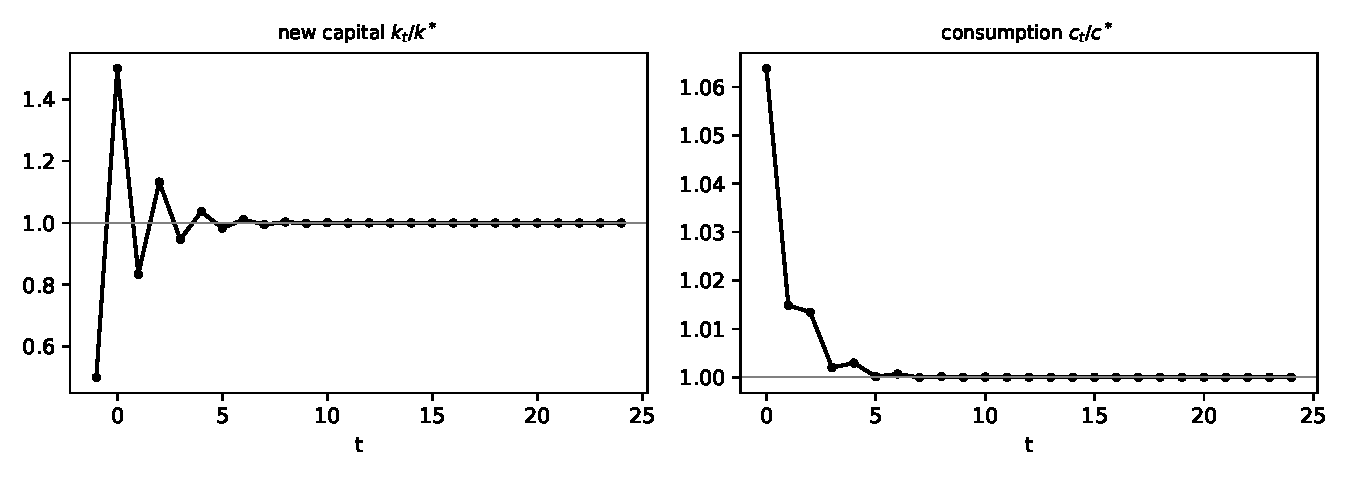
\includegraphics[width=0.85\textwidth]{figures/ch15_03.pdf}\\
{\small Figure S15.1. Optimal path from unequal initial vintages: damped echoes in investment, smooth consumption.}
\end{center}
So the researcher's claim is wrong for the stated economy: vintage-driven fluctuations are transitional, not permanent.
\end{ex}

%%---------------------------------------------------------------------------
\begin{ex}{15.4}{Excess capacity}
\textbf{(a)}  The planner maximizes $\sum\beta^tu(c_t)$ subject to $c_t+k_{t+1}=zf(\kappa_t)+k_t-\delta\kappa_t$ and $0\le\kappa_t\le k_t$.  Using a machine yields $zf'(\kappa)$ but costs $\delta$ in
depreciation, so utilization is chosen statically:
\[
  \kappa_t=\min\{k_t,\bar\kappa\},\qquad zf'(\bar\kappa)=\delta .
\]
All machines are used unless there are more than $\bar\kappa$, beyond which the marginal machine is worth more idle than in use.  The Euler equation for $k_{t+1}$ is
\[
  u'(c_t)=\beta u'(c_{t+1})\bigl[1+\lambda_{t+1}\bigr],\qquad \lambda_{t+1}=\begin{cases}zf'(k_{t+1})-\delta,&k_{t+1}\le\bar\kappa,\\0,&k_{t+1}>\bar\kappa.\end{cases}
\]
An idle machine earns a zero net return; since $\beta<1$, holding idle capacity would require consumption to fall over time.

\textbf{(b)}  In a steady state $\beta(1+\lambda)=1$, i.e.\ $\lambda=\rho>0$.  So capital cannot be partly idle, and $zf'(k^*)=\rho+\delta$.  This has a unique solution under the usual Inada
conditions, and it satisfies $k^*<\bar\kappa$ because $\rho+\delta>\delta$.

\textbf{(c)}  Full utilization: $\kappa^*=k^*$.  Idle capacity is optimal only in transition, when the economy starts with more capital than $\bar\kappa$.  Then the planner lets it sit idle
(undepreciated) and consumes out of output until the stock falls.

\textbf{(d)}  Not in steady state.  Every country uses all its capital, whatever its $z$.  Cross-country differences in $z$ show up in $k^*$ and $y^*$, not in utilization.  The model could
associate low output with low utilization only for economies far above their steady state, which is not the usual situation of poor countries.
\end{ex}

%%---------------------------------------------------------------------------
\begin{ex}{15.5}{Heterogeneity and growth}
\textbf{(a)}  A competitive equilibrium is a set of prices $\{r_t,w_t\}$ and allocations $\{c_{it},k_{i,t+1}\}$, $\{k_t\}$ such that: (1) given prices, each household maximizes
$\sum\beta^tu_i(c_{it})$ subject to $c_{it}+k_{i,t+1}=w_t+(1+r_t-\delta)k_{it}$ (plus a no-Ponzi condition); (2) firms maximize profits, $r_t=F_k(k_t,1)$ and $w_t=F_n(k_t,1)$, with zero profits
under constant returns; (3) markets clear: $k_t=\sum_ik_{it}$, labor $=1$, and $\sum_ic_{it}+k_{t+1}=F(k_t,1)+(1-\delta)k_t$.

\textbf{(b)(i)}  Each household's Euler equation is $u_i'(c_{it})=\beta(1+r_{t+1}-\delta)u_i'(c_{i,t+1})$.  In a steady state with constant prices, if $\beta(1+r-\delta)$ exceeded (fell short of) one,
\emph{every} household's consumption would grow (shrink) forever, contradicting a constant aggregate.  Hence $\beta(1+r-\delta)=1$, i.e.\ $F_k(k^*,1)=\rho+\delta$.  This determines $k^*$
and the interest rate uniquely, independently of the $u_i$.  A is right and B is wrong: the steady-state interest rate depends only on $\beta$ and $\delta$ (and $F$ gives $k^*$).

\textbf{(b)(ii)}  If $k_0=k^*$, prices are at their steady-state values from the start.  With $\beta(1+r-\delta)=1$ each household keeps its consumption, and hence its wealth, constant:
$c_i=w+(r-\delta)k_{i0}$.  Consumption inequality is an affine image of initial capital inequality, $c_i-c_j=(r-\delta)(k_{i0}-k_{j0})$, so A is right.  B is wrong.  Perfect capital
markets let households \emph{smooth} consumption, not equalize it, and nothing pushes wealth to converge.  For $k_0\ne k^*$, households with different intertemporal elasticities
respond differently during the transition, so the wealth distribution changes.  But long-run consumption still depends on initial wealth (and on the $u_i$), not on a common
level.

\textbf{(c)}  In each case aggregate capital and prices stay at their steady-state values, because lump-sum reallocations do not distort anyone's Euler equation and
$\beta(1+r-\delta)=1$ still holds.  Each household immediately moves to a new constant consumption equal to its new permanent income.
(i) After the redistribution, $c_i=w+(r-\delta)k_i^{\text{new}}$: consumption is redistributed accordingly, with no aggregate effects.
(ii) Permanent lump-sum taxes $T$ on one half and transfers on the other simply shift permanent incomes: the payers' consumption falls by $T$, the recipients' rises by the
corresponding transfer.  Aggregates are unchanged, since this is a pure redistribution.
(iii) The taxed two-thirds each reduce consumption by their tax.  Aggregate consumption falls by $g$ each period, while capital, output and the interest rate are unchanged: the
resources absorbed by $g$ come entirely out of the taxpayers' consumption.
\end{ex}

%%---------------------------------------------------------------------------
\begin{ex}{15.6}{Taxes and growth}
\textbf{(a)}  Taking $v_t$ as given, the planner's Euler equation is $u'(c_t)=\beta u'(c_{t+1})[(1-\tau)f'(k_{t+1})+1-\delta]$.  In equilibrium $v_t=\tau f(k_t)$, so the resource constraint is
$c_t+k_{t+1}=f(k_t)+(1-\delta)k_t-g$.  A steady state requires $(1-\tau)f'(k^*)=\rho+\delta$, which has a unique solution (since $f'$ decreases from $\infty$ to $0$), and
$c^*=f(k^*)-\delta k^*-g$, which we assume positive.  The equilibrium dynamics are those of the standard growth model, with the $\dot c=0$ locus at $k=k^*$ and the $\dot k=0$ locus
$c=f(k)-\delta k-g$.  Linearizing around the steady state, with $\tilde R\equiv f'(k^*)+1-\delta>1$ and
$b\equiv\beta(1-\tau)f''(k^*)u'(c^*)/u''(c^*)>0$, gives $dk_{t+1}=\tilde R\,dk_t-dc_t$ and $dc_{t+1}=dc_t-b\,dk_{t+1}$.  The Jacobian
$\begin{bmatrix}\tilde R&-1\\-b\tilde R&1+b\end{bmatrix}$ has characteristic polynomial $P(\lambda)=\lambda^2-(\tilde R+1+b)\lambda+\tilde R$, with $P(0)=\tilde R>0$ and $P(1)=-b<0$.  So one root lies in $(0,1)$ and the
other exceeds one: a saddle.  Paths above the stable arm hit $k=0$ in finite time, and paths below it violate the
transversality condition, so the equilibrium is the stable arm, which converges monotonically to $(k^*,c^*)$ from any $k_0>0$.

\textbf{(b)}  The new steady state has $(1-\tau')f'(k^{**})=\rho+\delta$, so $k^{**}>k^*$.  Output $f(k^{**})$ is higher, and consumption $c^{**}=f(k^{**})-\delta k^{**}-g>c^*$ because both steady
states lie below the golden rule ($f'>\delta$), where $f(k)-\delta k$ is increasing.  \emph{Transition}: capital is predetermined, so output does not jump at impact.  The new stable arm
passes below the old steady-state point (at $k=k^*<k^{**}$ it lies below the $\dot k=0$ locus, on which $c^*$ sits).  So consumption jumps down and investment jumps up.  Thereafter
$k_t$, $y_t$ and $c_t$ rise monotonically to their new steady-state values, and $c_t$ eventually exceeds the old $c^*$.  The transfer $v_t=\tau'f(k_t)$ falls at impact and then rises with
output; the second planner treats it as exogenous, which is exactly why the tax distorts saving.

\textbf{(c)}  With inelastic labor, the tax on labor income is effectively lump sum, and only the tax on capital income distorts.  The household Euler equation is
$u'(c_t)=\beta u'(c_{t+1})[1+(1-\tau)r_{t+1}-\delta]$ with $r=F_k(k,1)$, so in a steady state the \emph{after-tax} net return equals $\rho$:
$(1-\tau)r^*=\rho+\delta$.  The before-tax equilibrium interest rate $r^*=(\rho+\delta)/(1-\tau)$ therefore \emph{falls} with the tax cut, from $(\rho+\delta)/(1-\tau)$ to $(\rho+\delta)/(1-\tau')$, as capital
accumulates.  At impact $r_t$ is unchanged (capital is predetermined), and it then declines monotonically as $k_t$ rises.  The after-tax return $(1-\tau')r_t-\delta$ jumps up above $\rho$ at
impact, which is what makes consumption grow along the transition, and falls back to $\rho$ in the new steady state.
\end{ex}

%% ===========================================================================
%% Chapter 16. Optimal Taxation with Commitment
%% ===========================================================================
\solchapter{16}{Optimal Taxation with Commitment}

\begin{center}
\begin{minipage}{0.86\textwidth}
\small
Solutions to all 13 exercises of Chapter 16 of Ljungqvist and Sargent, \emph{Recursive Macroeconomic Theory} (4th edition, 2018).  Exercises 16.1--16.10 are analytical.
Exercises 16.11 and 16.12 leave preferences and the discount factor open, so we pick them.  The numbers for 16.5 and 16.11--16.13 come from \texttt{code/ch16.py}.
\end{minipage}
\end{center}

\bigskip
\hrule
\bigskip

\textbf{Notation.}  We use the primal approach of Section 16.5.  With the household's first-order conditions substituted into its present-value budget constraint, the
constraint becomes the \emph{implementability condition}
\[
  \sum_{t=0}^\infty\beta^t\bigl[u_c(t)c_t-u_\ell(t)n_t\bigr]=A,\qquad
  A=u_c(0)\bigl\{[(1-\tau^k_0)F_k(0)+1-\delta]k_0+b_0\bigr\}\quad\text{\bk{(16.5.5)--(16.5.6)}}.
\]
Let $V(c,n,\Phi)=u(c,1-n)+\Phi[u_cc-u_\ell n]$, and let $\theta_t$ be the multiplier on feasibility.  The Ramsey first-order conditions are \bk{(16.5.9)}: for $t\ge1$,
$V_c(t)=\beta V_c(t+1)[F_k(t+1)+1-\delta]$ and $V_n(t)=-V_c(t)F_n(t)$.  At $t=0$ they contain the extra terms $\Phi A_c$ and $\Phi A_n$.  A \emph{wedge} is the gap between a marginal
rate of substitution and the corresponding marginal rate of transformation.

%%---------------------------------------------------------------------------
\begin{ex}{16.1}{A small open economy (Razin and Sadka)}
\textbf{(a)}  A unit of capital owned between $t$ and $t+1$ earns the world gross return $R^*_t=r^*_{t+1}+1-\delta$, however it is used.  So the household's Arrow--Debreu prices
$q^0_t=\prod_{i<t}(R^*_i)^{-1}$ are exogenous, and its first-order conditions are
\[
  q^0_t=\beta^t\frac{u_c(t)}{u_c(0)},\qquad \frac{u_\ell(t)}{u_c(t)}=(1-\tau^n_t)w_t .
\]
Its present-value budget constraint is $\sum_tq^0_tc_t=\sum_tq^0_t(1-\tau^n_t)w_tn_t+a_0$, where $a_0$ is initial wealth (capital and bonds, including government debt $b_0$).
A domestic firm uses capital $k^d_t$ and sets $F_k(k^d_t,n_t)=(1+\hat\tau^k_t)r^*_t$ and $w_t=F_n(k^d_t,n_t)$.  Add the household's budget to the government's,
$\sum_tq^0_t[g_t-\tau^n_tw_tn_t-\hat\tau^k_tr^*_tk^d_t]=-b_0$, and use $F=F_kk^d+F_nn$.  The result is the \emph{national} present-value resource constraint
\[
  \sum_tq^0_t(c_t+g_t)=\sum_tq^0_t\bigl[F(k^d_t,n_t)-r^*_tk^d_t\bigr]+a_0-b_0 . \tag{i}
\]
Substituting the household's first-order conditions into its budget gives the implementability condition $\sum_t\beta^t[u_c(t)c_t-u_\ell(t)n_t]=u_c(0)a_0$ (ii).  The Euler
equations $\beta^tu_c(t)/u_c(0)=q^0_t$ (iii) are further restrictions on the allocation, because prices are fixed by the world market.  Conversely, any $\{c_t,n_t,k^d_t\}$ that
satisfies (i)--(iii) is a competitive equilibrium: set $w_t=F_n(k^d_t,n_t)$, read $\tau^n_t$ off $u_\ell/u_c=(1-\tau^n_t)w_t$ and $\hat\tau^k_t$ off
$F_k=(1+\hat\tau^k_t)r^*_t$.  The government's budget then holds by Walras' law.

So the Ramsey planner maximizes $\sum_t\beta^tu(c_t,1-n_t)$ subject to (i)--(iii).  The domestic capital stock $k^d_t$ appears \emph{only} in (i), through national net output
$F(k^d_t,n_t)-r^*_tk^d_t$.  It does not enter (ii), because any change in the pre-tax wage is absorbed by $\tau^n_t$.  Hence for any $(c,n)$ the planner maximizes net output,
\[
  F_k(k^d_t,n_t)=r^*_t\quad\Longrightarrow\quad \hat\tau^k_t=0\qquad\text{for all }t\ge0 .
\]
This includes $t=0$: domestic capital is not a fixed factor even at $t=0$, since firms can rent any amount at $r^*_0$.  This is the Diamond--Mirrlees production-efficiency
result.  A tax on capital used in domestic production is a tax on an intermediate input.  Capital's net return is fixed by the world market, so the whole burden of
$\hat\tau^k$ falls on the immobile factor, labor.  Taxing labor directly raises the same revenue without distorting production.

\textbf{(b)}  In the closed economy, capital income may be taxed (or subsidized) during the transition.  It is zero only in a steady state (\bk{Proposition 1}), and a tax on
the inelastic $k_0$ is a lump-sum levy, which is why $\tau^k_0$ must be bounded.  In the small open economy the supply of capital to domestic production is infinitely elastic
at $r^*_t$.  So the optimal capital tax is zero \emph{at every date}, not only asymptotically, and no capital levy is available.  Only labor is taxed.
\end{ex}

%%---------------------------------------------------------------------------
\begin{ex}{16.2}{Consumption taxes}
\textbf{(a)}  With multiplier $\lambda$ on the budget, the household's first-order conditions are $\beta^tu_c(t)=\lambda q^0_t(1+\tau^c_t)$ and
$\beta^tu_\ell(t)=\lambda q^0_t(1-\tau^n_t)w_t$.  Capital income is untaxed, so no arbitrage gives $q^0_t/q^0_{t+1}=F_k(t+1)+1-\delta$.  With $q^0_0=1$,
$\lambda=u_c(0)/(1+\tau^c_0)$.  Substituting into the budget gives the implementability condition
\[
  \sum_{t=0}^\infty\beta^t[u_c(t)c_t-u_\ell(t)n_t]=A^c,\qquad A^c=\frac{u_c(0)}{1+\tau^c_0}\bigl\{[F_k(0)+1-\delta]k_0+b_0\bigr\}.
\]
The Ramsey problem is (16.5.8) with $A$ replaced by $A^c$ and with $\tau^c_0$ given.  Its first-order conditions are (16.5.9a,b) for $t\ge1$.  At $t=0$,
$V_c(0)-\Phi A^c_c=\beta V_c(1)[F_k(1)+1-\delta]$ and $V_n(0)=[\Phi A^c_c-V_c(0)]F_n(0)+\Phi A^c_n$, together with feasibility and implementability.  Taxes are recovered from
the two wedges.  The intertemporal wedge (divide the first-order conditions at $t$ and $t+1$) gives
\[
  \frac{1+\tau^c_{t+1}}{1+\tau^c_t}=\frac{\beta u_c(t+1)[F_k(t+1)+1-\delta]}{u_c(t)},\qquad
  \frac{1-\tau^n_t}{1+\tau^c_t}=\frac{u_\ell(t)}{u_c(t)F_n(t)} .
\]
The first equation determines $\tau^c_{t+1}$ recursively from $\tau^c_0$, and the second then gives $\tau^n_t$.  There are two instruments for two wedges each period, so the
Ramsey taxes are unique once $\tau^c_0$ is fixed.

\textbf{(b)}  In a steady state $V_c$ is constant, so (16.5.9a) gives $\beta(F_k+1-\delta)=1$.  With $u_c$ constant, the first displayed formula gives
$(1+\tau^c_{t+1})/(1+\tau^c_t)\to1$: the \emph{consumption tax converges to a constant}.  A constant consumption tax does not distort the intertemporal margin, so this is the
counterpart of the zero limiting capital tax.  Its level, $1+\tau^c_\infty=(1+\tau^c_0)\prod_{t\ge0}\beta u_c(t+1)[F_k(t+1)+1-\delta]/u_c(t)$, reflects the transition.  In
the limit only the intratemporal wedge $(1-\tau^n_\infty)/(1+\tau^c_\infty)=u_\ell/(u_cF_n)$ distorts.

\textbf{(c)}  Take $\tau^c_t=\tau^c$ and $\tau^n_t=-\tau^c$ for all $t$.  Then $(1-\tau^n_t)/(1+\tau^c_t)=1$ and $(1+\tau^c_{t+1})/(1+\tau^c_t)=1$, so the household faces no
wedge at all.  Its budget becomes $(1+\tau^c)\sum_tq^0_t(c_t-w_tn_t)=W_0\equiv[r_0+1-\delta]k_0+b_0$, and the government collects, in present value,
\[
  \sum_tq^0_t\bigl[\tau^cc_t+\tau^n_tw_tn_t\bigr]=\tau^c\sum_tq^0_t(c_t-w_tn_t)=\frac{\tau^c}{1+\tau^c}\,W_0 .
\]
This policy is a lump-sum levy of the fraction $\tau^c/(1+\tau^c)$ of initial wealth (capital \emph{and} government debt), and that fraction tends to one as
$\tau^c\to\infty$.  A uniform consumption tax with an equal labor subsidy is thus a capital levy in disguise.  In the Ramsey problem, $\partial J/\partial\tau^c_0
=-\Phi\,\partial A^c/\partial\tau^c_0=\Phi A^c/(1+\tau^c_0)>0$ whenever $\Phi>0$ and $W_0>0$.  The planner would raise $\tau^c_0$ until $\Phi=0$ and then finance everything
without distortion.  Only $\tau^c_0$ enters $A^c$, so bounding $\tau^c_0$ is what keeps the problem interesting, exactly as bounding $\tau^k_0$ does in Section 16.6.
\end{ex}

%%---------------------------------------------------------------------------
\begin{ex}{16.3}{A specific utility function (Chamley)}
\textbf{(a)}  Here $u_cc=c^{1-\sigma}$ and $u_\ell$ does not depend on $c$, so $V=u+\Phi[c^{1-\sigma}-v'(\ell)n]$ and
\[
  V_c=u_c+\Phi(1-\sigma)c^{-\sigma}=[1+\Phi(1-\sigma)]\,u_c .
\]
The factor $1+\Phi(1-\sigma)$ is positive, because $V_c(t)=\theta_t$, the shadow value of goods.  Dividing (16.5.9a) by it gives, for $t\ge1$,
$u_c(t)=\beta u_c(t+1)[F_k(t+1)+1-\delta]$.  The household's Euler equation (16.5.4), with $q^0_t/q^0_{t+1}=u_c(t)/[\beta u_c(t+1)]$, is
$u_c(t)=\beta u_c(t+1)[(1-\tau^k_{t+1})F_k(t+1)+1-\delta]$.  Subtracting, $\tau^k_{t+1}F_k(t+1)=0$, so $\tau^k_{t+1}=0$ for $t\ge1$, i.e.\ $\tau^k_t=0$ for all $t\ge2$.
Only $\tau^k_1$ can differ from zero, because the $t=0$ condition (16.5.9c) contains $\Phi A_c$.

\textbf{(b)}  In the stochastic model, (16.10.4a) gives $V_c(s^t)=\beta E_tV_c(s^{t+1})[F_k(s^{t+1})+1-\delta]$ for $t\ge1$.  With $V_c=[1+\Phi(1-\sigma)]u_c$ this is
$u_c(s^t)=\beta E_tu_c(s^{t+1})[F_k(s^{t+1})+1-\delta]$.  The household's condition (16.8.5c) is $u_c(s^t)=\beta E_tu_c(s^{t+1})[(1-\tau^k_{t+1}(s^{t+1}))F_k(s^{t+1})+1-\delta]$.
Subtracting,
\[
  E_t\bigl[u_c(s^{t+1})\tau^k_{t+1}(s^{t+1})F_k(s^{t+1})\bigr]=0
  \quad\Longrightarrow\quad
  \bar\tau^k_{t+1}(s^t)=\frac{E_tu_c(s^{t+1})\tau^k_{t+1}(s^{t+1})r_{t+1}(s^{t+1})}{E_tu_c(s^{t+1})r_{t+1}(s^{t+1})}=0
\]
by (16.9.5) and (16.11.1).  The ex ante capital tax is zero for all $t\ge2$.  Realized state-by-state rates are not pinned down (Section 16.9); only their $u_cF_k$-weighted
average is.  This is the case $\Lambda=1+\Phi(1-\sigma)$ of \bk{Proposition 2}.
\end{ex}

%%---------------------------------------------------------------------------
\begin{ex}{16.4}{Two labor inputs (Jones, Manuelli, and Rossi)}
\textbf{(a)}  The household sets $u_\ell(t)=u_c(t)(1-\tau^n_{it})w_{it}$ for $i=1,2$.  Both kinds of work cost the same leisure, so after-tax wages are equal:
$(1-\tau^n_{1t})w_{1t}=(1-\tau^n_{2t})w_{2t}$.  The implementability condition is $\sum_t\beta^t[u_cc-u_\ell(n_1+n_2)]=A$, with
$A=u_c(0)W_0$ and $W_0=[(1-\tau^k_0)F_k(0)+1-\delta]k_0+b_0$.  So $V=u(c,1-n_1-n_2)+\Phi[u_cc-u_\ell(n_1+n_2)]$ depends on $(n_1,n_2)$ only through $n_1+n_2$, and
$V_{n_1}=V_{n_2}\equiv V_n$.  In the Lagrangian $J=\sum_t\beta^t\{V_t+\theta_t[F(k_t,n_{1t},n_{2t})+(1-\delta)k_t-c_t-g_t-k_{t+1}]\}-\Phi A$ the first-order conditions for
$n_{it}$, $t\ge1$, are $V_n(t)+\theta_tF_{n_i}(t)=0$ for $i=1,2$.  Hence $F_{n_1}(t)=F_{n_2}(t)$, i.e.\ $w_{1t}=w_{2t}$, and equal after-tax wages give
\[
  \tau^n_{1t}=\tau^n_{2t}\qquad(t\ge1).
\]
The two labor types are perfect substitutes in utility.  Only total hours should be distorted, and the production margin between the two types should not
(production efficiency).  At $t=0$ the conditions are $V_n(0)+\theta_0F_{n_i}(0)-\Phi A_{n_i}=0$, with
$A_{n_i}=-u_{c\ell}(0)W_0+u_c(0)(1-\tau^k_0)F_{kn_i}(0)k_0$.  The first term is common to $i=1,2$, so subtracting,
\[
  \theta_0\bigl[F_{n_1}(0)-F_{n_2}(0)\bigr]=\Phi\,u_c(0)(1-\tau^k_0)k_0\bigl[F_{kn_1}(0)-F_{kn_2}(0)\bigr].
\]
With $F_{kn_1}>0>F_{kn_2}$, $\Phi>0$ and $\tau^k_0<1$, the right side is positive.  So $w_{10}>w_{20}$, and equal after-tax wages then require
$\tau^n_{10}>\tau^n_{20}$.  The reason is that at $t=0$ the planner wants to shrink the value $A$ of initial wealth, which includes the untaxed part of capital's rental
$F_k(0)k_0$.  Discouraging $n_1$ (a complement of $k$) and encouraging $n_2$ (a substitute) lowers $F_k(0)$, which works like a partial levy on the inelastic $k_0$.  From
$t=1$ on, capital is no longer a fixed factor and the motive disappears.

\textbf{(b)}  The household sets $u_{\ell_i}(t)=u_c(t)(1-\tau^n_t)w_{it}$.  The common tax rate is equivalent to $u_{\ell_1}/F_{n_1}=u_{\ell_2}/F_{n_2}$, i.e.\ to
$G_t\equiv u_{\ell_1}(t)F_{n_2}(t)-u_{\ell_2}(t)F_{n_1}(t)=0$.  The implementability condition is $\sum_t\beta^t[u_cc-u_{\ell_1}n_1-u_{\ell_2}n_2]=A$, and
$V=u+\Phi[u_cc-u_{\ell_1}n_1-u_{\ell_2}n_2]$.  With multipliers $\theta_t$ on feasibility and $\eta_t$ on $G_t=0$, the first-order conditions for $t\ge1$ are
\begin{align*}
  c_t:&\quad V_c(t)+\eta_tG_c(t)=\theta_t,\\
  n_{it}:&\quad V_{n_i}(t)+\theta_tF_{n_i}(t)+\eta_tG_{n_i}(t)=0,\quad i=1,2,\\
  k_{t+1}:&\quad \theta_t=\beta\bigl\{\theta_{t+1}[F_k(t+1)+1-\delta]+\eta_{t+1}G_k(t+1)\bigr\},\qquad G_k=u_{\ell_1}F_{n_2k}-u_{\ell_2}F_{n_1k}.
\end{align*}
The $t=0$ conditions add the derivatives of $-\Phi A$.  Together with feasibility, implementability and $G_t=0$, these determine the allocation.  The taxes then follow from
$u_{\ell_1}=u_c(1-\tau^n_t)F_{n_1}$ and $u_c(t)=\beta u_c(t+1)[(1-\tau^k_{t+1})F_k(t+1)+1-\delta]$.  Note that $\eta_t$ appears in the capital condition: capital
changes the relative wage $F_{n_1}/F_{n_2}$, and hence how tight the equal-tax restriction is.

\textbf{(c)}  In a steady state, the $k$ condition is $1=\beta(F_k+1-\delta)+\beta\eta G_k/\theta$, and the household's Euler equation is $1=\beta[(1-\tau^k)F_k+1-\delta]$.
Subtracting, $\tau^kF_k=-\eta G_k/\theta$.  Using $u_{\ell_2}=u_{\ell_1}F_{n_2}/F_{n_1}$ from the constraint,
\[
  \tau^k=-\frac{\eta\,u_{\ell_1}}{\theta\,F_k\,F_{n_1}}\,\bigl[F_{n_1}F_{n_2k}-F_{n_2}F_{n_1k}\bigr].
\]
If the restriction binds ($\eta\ne0$), the limiting capital tax is zero if and only if $F_{n_1}F_{n_2k}=F_{n_2}F_{n_1k}$, i.e.\
$\partial(F_{n_1}/F_{n_2})/\partial k=0$.  When capital moves the relative wage, the planner taxes or subsidizes capital to steer relative wages, as a substitute for
the differential labor taxation it is not allowed to use.  This matches the incomplete-taxation logic of Section 16.7.
\end{ex}

%%---------------------------------------------------------------------------
\begin{ex}{16.5}{Another specific utility function}
\textbf{(a)}  With multiplier $\beta^t\lambda_t$ on the date-$t$ budget, the condition for $c_t$ is $1=\lambda_t$.  The one for $b_{t+1}$ is $\lambda_tq_t=\beta\lambda_{t+1}$, so
$q_t=\beta$.  The one for leisure is $u_x=1-x_t=\lambda_t(1-\tau_t)$, so $x_t=\tau_t$.

\textbf{(b)}  Since $u_c=1>0$, the budget holds with equality.  Multiply the date-$t$ budget by $\beta^t$, use $q_t=\beta$, and sum from $0$ to $T$.  The bond terms
telescope, giving $\sum_{t=0}^T\beta^t[c_t-(1-\tau_t)(1-x_t)]+\beta^{T+1}b_{T+1}=b_0=0$.  Let $T\to\infty$.

\textbf{(c)}  Substitute $x_t=\tau_t$ and $c_t=1-\tau_t-g_t$.  Period utility becomes $1-\tau_t-g_t-.5(1-\tau_t)^2=.5-.5\tau_t^2-g_t$, and the budget becomes
$\sum_t\beta^t\tau_t(1-\tau_t)=G\equiv\sum_t\beta^tg_t$.  So the planner minimizes $\sum_t\beta^t\tau_t^2$ subject to $\sum_t\beta^t(\tau_t-\tau_t^2)=G$.  The Lagrangian
condition $-\tau_t+\mu(1-2\tau_t)=0$ gives $\tau_t=\mu/(1+2\mu)$, the same at every date whatever $g_t$ is.  The constant $\tau$ is also the \emph{global} optimum.  Let
$S_1=(1-\beta)\sum\beta^t\tau_t$ and $S_2=(1-\beta)\sum\beta^t\tau_t^2$.  The constraint is $S_2=S_1-\bar g$ with $\bar g=(1-\beta)G$, and Jensen's inequality gives
$S_2\ge S_1^2$.  Hence $S_1^2-S_1+\bar g\le0$, so $S_1\ge\tau_-$, the smaller root of $\tau(1-\tau)=\bar g$.  Therefore $S_2=S_1-\bar g\ge\tau_--\bar g=\tau_-^2$, with
equality only if $\tau_t\equiv\tau_-$.  Thus
\[
  \tau(1-\tau)=(1-\beta)\sum_{t\ge0}\beta^tg_t,\qquad \tau=\tfrac12\bigl[1-\sqrt{1-4(1-\beta)G}\,\bigr].
\]
Here $G=.2\beta/(1-\beta^2)$, so $(1-\beta)G=.2\beta/(1+\beta)=.097436$ and $\tau=.109405$.  The other root, $.890595$, raises the same revenue on the wrong side of the
Laffer curve.

\textbf{(d)}  Now $G=.2/(1-\beta^2)$, so $(1-\beta)G=.2/(1+\beta)=.102564$ and $\tau=.116026$.  This is larger than in (c): the same purchases come one period earlier, so
their present value, and the annuity the tax must finance, are higher by the factor $1/\beta$.

\textbf{(e)}  The tax rate is constant even though purchases alternate between $0$ and $.2$.  Debt absorbs the fluctuations.  Since $b_{t+1}=[b_t+g_t-\tau(1-\tau)]/\beta$, in
(c) the government saves in the low-purchase periods ($b_1=-\tau(1-\tau)/\beta=-.102564$) and spends the savings in the high ones ($b_2=0$), and so on.  In (d) it borrows
$.102564$ in each high-purchase period and repays in the next.  The deadweight loss is convex in the tax rate ($.5\tau^2$ per period), so it is cheapest to spread it
evenly over time: tax smoothing (Barro).

\textbf{(f)}  $\tau=0$ exactly when no revenue is needed, i.e.\ when $\sum_t\beta^tg_t=0$: $g_t=0$ for all $t$ (with $b_0=0$).  More generally, with initial debt $b_0$ the
condition is $\tau(1-\tau)=(1-\beta)(G+b_0)$.  Then $\tau=0$ if the government's initial assets $-b_0$ exactly cover the present value of its purchases.
\end{ex}

%%---------------------------------------------------------------------------
\begin{ex}{16.6}{Yet another specific utility function}
\exnote{Equations (1), (4) and (5) refer to the numbered displays of the exercise in the book.}
\textbf{(a)}  A competitive equilibrium with taxes is an allocation $\{c_t,n_t\}$, a price system $\{q_t\}$ and a budget-feasible tax sequence $\{\tau_t\}$ (one that satisfies
(5)) such that: (i) given $\{q_t,\tau_t\}$, the allocation maximizes (1) subject to (4); and (ii) $n_t=c_t+g_t$ for all $t$.  The household's first-order conditions (interior
$n_t$) are $\beta^t=\lambda q_t$ and $\beta^t(u_1+u_2n_t)=\lambda q_t(1-\tau_t)$.  With $q_0=1$,
\[
  q_t=\beta^t,\qquad n_t=\frac{1-u_1-\tau_t}{u_2}\quad\text{i.e. }\tau_t=1-u_1-u_2n_t .
\]

\textbf{(b)}  Because $\tau_t=1-u_1-u_2n_t$, the planner effectively chooses $\{n_t\}$ to maximize $\sum_t\beta^t[(1-u_1)n_t-.5u_2n_t^2-g_t]$ subject to
$\sum_t\beta^t[(1-u_1-u_2n_t)n_t-g_t]=0$.  With multiplier $\mu$, the first-order condition is $(1-u_1-u_2n_t)+\mu(1-u_1-2u_2n_t)=0$, so
\[
  n_t=\bar n=\frac{(1+\mu)(1-u_1)}{(1+2\mu)u_2},\qquad \tau_t=\tau=1-u_1-u_2\bar n=\frac{\mu}{1+2\mu}(1-u_1),
\]
constant over time and independent of $g_t$.  The budget $\tau\bar n/(1-\beta)=G\equiv\sum\beta^tg_t$ gives
$\tau(1-u_1-\tau)=u_2(1-\beta)G$, so $\tau=\tfrac12\bigl[(1-u_1)-\sqrt{(1-u_1)^2-4u_2(1-\beta)G}\bigr]$.  A solution exists iff $(1-u_1)^2\ge4u_2(1-\beta)G$.  As in 16.5,
Jensen's inequality shows the constant plan is globally optimal.  Write $S_1=(1-\beta)\sum\beta^tn_t$, $S_2=(1-\beta)\sum\beta^tn_t^2$ and $\bar g=(1-\beta)G$.  On the
constraint set $(1-u_1)S_1-u_2S_2=\bar g$ the objective equals $(1-\beta)^{-1}[\bar g+.5u_2S_2]-G$, so the planner maximizes $S_2$.  Now $S_2\ge S_1^2$ forces
$u_2S_1^2-(1-u_1)S_1+\bar g\le0$, i.e.\ $S_1\le n_+$, the larger root.  Hence $S_2=[(1-u_1)S_1-\bar g]/u_2\le n_+^2$, with equality iff $n_t\equiv n_+=\bar n$.  Prices are $q_t=\beta^t$, so the gross interest rate is $1/\beta$
at every date.  Consumption $c_t=\bar n-g_t$ absorbs all fluctuations in $g_t$.  The tax rate and labor supply are perfectly smoothed, and debt finances the difference
between constant revenue $\tau\bar n$ and fluctuating purchases.

\textbf{(c)}  $G_A=\beta g/(1-\beta^2)$ and $G_B=\beta g\cdot1/(1-\beta^2)$ are equal.  Since $\tau$ depends on $\{g_t\}$ only through $G$, both sequences have the \emph{same}
Ramsey tax rate, labor supply $\bar n$ and interest rates ($q_t=\beta^t$, gross rate $1/\beta$).  They differ only in consumption, $c_t=\bar n-g_t$, and in the debt path.
Under A the government runs a surplus $\tau\bar n=\beta g/(1+\beta)$ at even dates, saving $b_{2j+1}=-g/(1+\beta)$, and spends the savings at odd dates.  Under B it borrows
$b_{2j+1}=\beta g/(1+\beta)$ at even dates and repays at odd dates.
\end{ex}

%%---------------------------------------------------------------------------
\begin{ex}{16.7}{Comparison of tax systems}
The book writes the capital-tax revenue as $\tau^a_t(r_{t+1}-\delta)k_t$.  Since $k_t$ is the capital used, and rented at $r_t$, in period $t$, we read it as
$\tau^a_t(r_t-\delta)k_t$.
\rmk{The date index $r_{t+1}$ in the book's revenue formula appears to be a misprint for $r_t$.}

\textbf{(a)}  Economy 1.  The household's budget is $c_t+k_{t+1}+b_{t+1}/R_t=(1-\tau^n_t)w_tn_t+[1+(1-\tau^a_t)(r_t-\delta)]k_t+b_t$.  Its first-order conditions are
\[
  \frac{u_\ell(t)}{u_c(t)}=(1-\tau^n_t)w_t,\qquad u_c(t)=\beta u_c(t+1)\bigl[1+(1-\tau^a_{t+1})(r_{t+1}-\delta)\bigr],
\]
with $q^0_t=\beta^tu_c(t)/u_c(0)$.  Substituting into the present-value budget, with $b_0=0$ and $\tau^a_0=0$, gives the implementability condition
\[
  \sum_{t\ge0}\beta^t[u_c(t)c_t-u_\ell(t)n_t]=A\equiv u_c(0)[1+F_k(0)-\delta]k_0 .
\]
The restriction $\tau^n_0=0$ adds the constraint $u_\ell(0)=u_c(0)F_n(k_0,n_0)$: time-0 labor is undistorted.  The Ramsey problem maximizes $\sum\beta^tu(c_t,1-n_t)$
subject to feasibility, implementability and this date-0 constraint.  With multipliers $\theta_t$, $\Phi$ and $\nu$, the Lagrangian is
$J=\sum_t\beta^t\{V(c_t,n_t,\Phi)+\theta_t[F(k_t,n_t)+(1-\delta)k_t-c_t-g_t-k_{t+1}]\}-\Phi A+\nu[u_\ell(0)-u_c(0)F_n(0)]$.  For $t\ge1$ its first-order conditions are exactly
(16.5.9a,b).  The date-0 conditions contain $\Phi A_c,\Phi A_n$ and the $\nu$ terms.  Taxes follow from $1-\tau^n_t=u_\ell(t)/[u_c(t)F_n(t)]$ and
$u_c(t)=\beta u_c(t+1)[1+(1-\tau^a_{t+1})(F_k(t+1)-\delta)]$.

\textbf{(b)}  In a steady state (16.5.9a) gives $\beta(1+F_k-\delta)=1$, and the Euler equation gives $\beta[1+(1-\tau^a)(F_k-\delta)]=1$.  Hence $\tau^a(F_k-\delta)=0$.
Since $F_k-\delta=1/\beta-1>0$, $\tau^a_\infty=0$.

\textbf{(c)}  Economy 2.  Let $\tilde q_t$ be the date-0 price of pre-tax goods.  Consumption is taxed but investment is not.  The household's first-order conditions are
$\beta^tu_c(t)=\tilde\lambda\tilde q_t(1+\tilde\tau^c_t)$ and $\beta^tu_\ell(t)=\tilde\lambda\tilde q_tw_t$, with no-arbitrage
$\tilde q_{t-1}=\tilde q_t[1+(1-\tilde\tau^a_t)(r_t-\delta)]$.  So
\[
  \frac{u_\ell(t)}{u_c(t)}=\frac{w_t}{1+\tilde\tau^c_t},\qquad
  \frac{u_c(t)}{1+\tilde\tau^c_t}=\beta\frac{u_c(t+1)}{1+\tilde\tau^c_{t+1}}\bigl[1+(1-\tilde\tau^a_{t+1})(r_{t+1}-\delta)\bigr].
\]
With $\tilde q_0=1$ and $\tilde\tau^c_0=0$, $\tilde\lambda=u_c(0)$.  The budget $\sum\tilde q_t(1+\tilde\tau^c_t)c_t=\sum\tilde q_tw_tn_t+[1+r_0-\delta]k_0$ becomes
$\sum\beta^t[u_cc-u_\ell n]=u_c(0)[1+F_k(0)-\delta]k_0=A$, the \emph{same} implementability condition.  The restriction $\tilde\tau^c_0=0$ again means
$u_\ell(0)=u_c(0)F_n(0)$.  So the Ramsey problem of economy 2 has the same objective and the same constraints on the allocation as that of economy 1.

\textbf{(d)}  The two Ramsey problems are identical as problems in $\{c_t,n_t,k_{t+1}\}$.  So (with a unique solution) $\tilde c_t=c_t$, $\tilde n_t=n_t$,
$\tilde\ell_t=\ell_t$ and $\tilde k_{t+1}=k_{t+1}$ for all $t$, and the factor prices $r_t,w_t$ coincide.

\textbf{(e)}  Match the two wedges at the common allocation.  Intratemporally, $1/(1+\tilde\tau^c_t)=1-\tau^n_t$, so
\[
  \tilde\tau^c_t=\frac{\tau^n_t}{1-\tau^n_t}.
\]
Intertemporally, $(1+\tilde\tau^c_t)/(1+\tilde\tau^c_{t+1})=(1-\tau^n_{t+1})/(1-\tau^n_t)$, so
\[
  1+(1-\tilde\tau^a_{t+1})(r_{t+1}-\delta)=\frac{1-\tau^n_t}{1-\tau^n_{t+1}}\bigl[1+(1-\tau^a_{t+1})(r_{t+1}-\delta)\bigr],
\]
i.e.\ $\tilde\tau^a_{t+1}=\{(1+r_{t+1}-\delta)-\rho_t[1+(1-\tau^a_{t+1})(r_{t+1}-\delta)]\}/(r_{t+1}-\delta)$ with $\rho_t=(1-\tau^n_t)/(1-\tau^n_{t+1})$.  Besides the
tax rates, this involves only the return $r_{t+1}-\delta$, which is common to the two economies.  When $\tau^n_{t+1}=\tau^n_t$ it reduces to
$\tilde\tau^a_{t+1}=\tau^a_{t+1}$.  If labor taxes rise over time ($\rho_t>1$), economy 2 must tax capital less, because a rising consumption tax already penalizes saving.
Asymptotically, $\tilde\tau^c_\infty=\tau^n_\infty/(1-\tau^n_\infty)$ and $\tilde\tau^a_\infty=\tau^a_\infty=0$.

\textbf{(f)}  In economy 1, $\mathrm{Gov}_1\equiv\sum_tq_t[\tau^n_tw_tn_t+\tau^a_t(r_t-\delta)k_t-g_t]=0$, with $q_t=q^0_t$.  By no arbitrage,
$q_t\tau^a_t(r_t-\delta)k_t=q_t(1+r_t-\delta)k_t-q_{t-1}k_t$ for $t\ge1$ ($\tau^a_0=0$).  By feasibility, $g_t=w_tn_t+(1+r_t-\delta)k_t-c_t-k_{t+1}$.  Substituting, the
capital terms telescope (using the transversality condition), and
\[
  \mathrm{Gov}_1=\sum_tq_tc_t-\sum_tq_t(1-\tau^n_t)w_tn_t-(1+r_0-\delta)k_0 .
\]
The same steps in economy 2 give
$\mathrm{Gov}_2\equiv\sum_t\tilde q_t[\tilde\tau^c_tc_t+\tilde\tau^a_t(r_t-\delta)k_t-g_t]=\sum_t\tilde q_t(1+\tilde\tau^c_t)c_t-\sum_t\tilde q_tw_tn_t-(1+r_0-\delta)k_0$.
By (d) and (e), $\tilde q_t(1+\tilde\tau^c_t)=\beta^tu_c(t)/u_c(0)=q_t$, and hence $\tilde q_t=q_t(1-\tau^n_t)$ and $\tilde q_tw_t=q_t(1-\tau^n_t)w_t$.  Therefore
$\mathrm{Gov}_2=\mathrm{Gov}_1$ term by term: economy 1's budget at $\Omega$ \emph{is} economy 2's budget at $\tilde\Omega$.  (Each also equals minus the slack in the
corresponding household budget, which is Walras' law.)
\end{ex}

%%---------------------------------------------------------------------------
\begin{ex}{16.8}{Taxes on capital, labor, and consumption, I}
\textbf{(a)}  The first-order conditions are $\beta^tu_c=\lambda q^0_t(1+\tau^c_t)$ and $\beta^tu_\ell=\lambda q^0_t(1-\tau^n_t)w_t$, with no arbitrage
$q^0_t/q^0_{t+1}=(1-\tau^k_{t+1})r_{t+1}+1-\delta$ and $\lambda=u_c(0)/(1+\tau^c_0)$.  The implementability condition is
$\sum\beta^t[u_cc-u_\ell n]=A$, with
\[
  A=\frac{u_c(0)}{1+\tau^c_0}\bigl\{[(1-\tau^k_0)F_k(0)+1-\delta]k_0+b_0\bigr\}.
\]
$A$ falls when either $\tau^c_0$ or $\tau^k_0$ rises, and $\partial J/\partial A=-\Phi<0$, so both are set at their upper bounds.  Given them, the Ramsey allocation solves
(16.5.9)--(16.5.10).  For $t\ge1$ the allocation pins down only two wedges per period:
\[
  \frac{1-\tau^n_t}{1+\tau^c_t}=\frac{u_\ell(t)}{u_c(t)F_n(t)},\qquad
  \frac{1+\tau^c_t}{1+\tau^c_{t+1}}\bigl[(1-\tau^k_{t+1})F_k(t+1)+1-\delta\bigr]=\frac{u_c(t)}{\beta u_c(t+1)} .
\]
There are three instruments for two wedges, so the \emph{Ramsey tax system is not unique}: one instrument per period can be chosen freely.  For example, one can hold
$\tau^c_t$ at its date-0 value and use $(\tau^n_t,\tau^k_{t+1})$ as in the text.  Or one can set $\tau^k_t=0$ for $t\ge1$ and let a time-varying $\tau^c_t$ deliver the
intertemporal wedge.  Debt adjusts, and the government's budget holds by Walras' law.

\textbf{(b)}  Let $\hat r_t=F_k(\hat k_t,\hat n_t)$, $\hat R_t=(1-\hat\tau^k)\hat r_t+1-\delta$ and $W(\tau)=[(1-\tau)\hat r_0+1-\delta]k_0+b_0$.  Define
\begin{align*}
  1+\tau^c_0&=\frac{W(0)}{W(\hat\tau^k)},\qquad
  1+\tau^c_t=(1+\tau^c_0)\prod_{j=1}^{t}\frac{\hat r_j+1-\delta}{(1-\hat\tau^k)\hat r_j+1-\delta}\quad(t\ge1),\\
  1-\tau^n_t&=(1-\hat\tau^n)(1+\tau^c_t)\quad(t\ge0),\qquad \tau^k_t=0\quad(t\ge0).
\end{align*}
\emph{The household's conditions hold.}  Intratemporally, $(1-\tau^n_t)/(1+\tau^c_t)=1-\hat\tau^n$, as before.  Intertemporally,
$[(1+\tau^c_t)/(1+\tau^c_{t+1})](\hat r_{t+1}+1-\delta)=\hat R_{t+1}$, as before.
\emph{The budget set is the same.}  The new prices of pre-tax goods satisfy $q'_t/q'_{t+1}=\hat r_{t+1}+1-\delta$, so $q'_t(1+\tau^c_t)=(1+\tau^c_0)\hat q_t$, where
$\hat q_t=\prod_{j\le t}\hat R_j^{-1}$ are the old prices, and $q'_t(1-\tau^n_t)=(1+\tau^c_0)(1-\hat\tau^n)\hat q_t$.  The new budget
$\sum q'_t(1+\tau^c_t)c_t=\sum q'_t(1-\tau^n_t)w_tn_t+W(0)$ is then the old one, $\sum\hat q_tc_t=\sum\hat q_t(1-\hat\tau^n)w_tn_t+W(\hat\tau^k)$, multiplied by
$1+\tau^c_0$.  So the household chooses the same allocation.  Feasibility is unchanged, and the government's present-value budget holds by Walras' law, with a different
debt path.  If $\hat\tau^k>0$, the date-0 consumption tax is positive.  It replaces the part of the time-0 capital levy that $\hat\tau^k$ imposed on $k_0$.

\textbf{(c)}  With $\hat\tau^k>0$, each factor in the product exceeds one.  The equivalent consumption tax rises geometrically (at the steady-state rate
$(\hat r+1-\delta)/\hat R$), and $1-\tau^n_t$ rises with it, so the labor tax falls and becomes an ever larger subsidy.  A constant capital tax is thus an ever-growing tax on
consumption (and on leisure) at later dates relative to earlier ones.  The intertemporal wedge between $c_0$ and $c_t$ grows without bound as $t\to\infty$, while the
intratemporal wedge between $c_t$ and $\ell_t$ stays at $1-\hat\tau^n$.

\textbf{(d)}  The Ramsey plan satisfies both lessons asymptotically: $\tau^k_\infty=0$, i.e.\ $(1+\tau^c_{t+1})/(1+\tau^c_t)\to1$ (no intertemporal wedge), and
$(1-\tau^n_t)/(1+\tau^c_t)$ converges to a constant.  The policy of (b) obeys lesson 2 exactly but violates lesson 1 more and more over time, which is why it is not
optimal.  The lessons concern wedges on the final goods $(c_t,\ell_t)$, not particular instruments: a ``capital tax'' can be relabeled as a rising consumption tax plus
a falling labor tax.
\end{ex}

%%---------------------------------------------------------------------------
\begin{ex}{16.9}{Taxes on capital, labor, and consumption, II}
\textbf{(a)}  As in 16.8(a): both date-0 taxes are at their upper bounds $\bar\tau^k_0,\bar\tau^c_0$, and the allocation solves (16.5.9)--(16.5.10) with $A$ evaluated at
the bounds.  The tax system is not unique, since there are three instruments for two wedges per period.

\textbf{(b)}  This part only introduces the benchmark policy and its allocation; nothing needs to be derived.

\textbf{(c)}  Yes, provided the frozen rate is compatible with the date-0 restriction, i.e.\ $\hat\tau^k=\bar\tau^k_0$ (the frozen rate uses the capital levy allowed at
$t=0$).  Let $\{c_t,n_t,k_{t+1}\}$ be the Ramsey allocation.  Set $\tau^c_0=\bar\tau^c_0$ and $\tau^k_t=\hat\tau^k$, and define recursively
\[
  1+\tau^c_{t+1}=(1+\tau^c_t)\,\frac{\beta u_c(t+1)\bigl[(1-\hat\tau^k)F_k(t+1)+1-\delta\bigr]}{u_c(t)},\qquad
  1-\tau^n_t=(1+\tau^c_t)\frac{u_\ell(t)}{u_c(t)F_n(t)} .
\]
Then both wedge conditions of 16.8(a) hold at the Ramsey allocation.  $A$ has the Ramsey value, so implementability holds, and the allocation is a competitive equilibrium
under this policy.  It is therefore a Ramsey policy.  If instead $\hat\tau^k<\bar\tau^k_0$, freezing $\tau^k_0=\hat\tau^k$ forgoes part of the date-0 levy.  Since
$\tau^c_0$ is already at its bound, $A$ is larger than in the Ramsey plan, and the Ramsey allocation of (a) cannot be reached.  The class then implements only the Ramsey
plan of the problem with $\tau^k_0=\hat\tau^k$ taken as given.  Along the Ramsey path, $\beta(F_k+1-\delta)\to1$ and $u_c$ converges, so
\[
  \frac{1+\tau^c_{t+1}}{1+\tau^c_t}\to\frac{(1-\hat\tau^k)F_k+1-\delta}{F_k+1-\delta}<1\qquad(\hat\tau^k>0).
\]
The consumption tax declines geometrically, with $1+\tau^c_t\to0$, and $1-\tau^n_t$ falls in proportion, so labor taxes rise toward 100\%.

\textbf{(d)}  The declining consumption tax subsidizes future consumption at exactly the rate that undoes the capital tax's penalty on saving.  So the Ramsey plan's
intertemporal wedge on $(c_t,c_{t+1})$ still vanishes in the limit (lesson 1).  The labor tax moves in step with $1+\tau^c_t$ so that the intratemporal wedge
$(1-\tau^n_t)/(1+\tau^c_t)=u_\ell/(u_cF_n)$ converges to a constant (lesson 2).  Any single instrument can be frozen, as long as the remaining two can still produce both
wedges.  The lessons restrict wedges, not tax rates.
\end{ex}

%%---------------------------------------------------------------------------
\begin{ex}{16.10}{The Lucas and Stokey (1983) model}
\textbf{(a)}  Here $w_t=1$, $u_c=1$ and $u_\ell=H'(\ell)$.  The household's conditions are $H'(\ell_t)=1-\tau^n_t$ and $p_t(s_{t+1}|s^t)=\beta\pi(s_{t+1}|s^t)$.  The
implementability condition (16.12.2), with $c_t=1-\ell_t-g_t$, reads
\[
  \sum_t\sum_{s^t}\beta^t\pi_t(s^t)\bigl[(1-\ell_t)(1-H'(\ell_t))-g_t\bigr]=b_0 .
\]
The Ramsey problem is to maximize $\sum\beta^t\pi_t[1-\ell_t-g_t+H(\ell_t)]$ subject to it.  Since $u_{cc}=u_{c\ell}=0$, the date-0 terms $\Phi u_{cc}b_0$ and
$\Phi u_{c\ell}b_0$ in (16.12.3c,d) vanish.  The first-order condition is the same at \emph{every} $t$ and $s^t$, including $t=0$:
\[
  (1+\Phi)\bigl[H'(\ell)-1\bigr]=\Phi\,(1-\ell)H''(\ell).
\]
It involves neither $t$, $s^t$ nor $g$, so $\ell_t(s^t)=\bar\ell(\Phi)$ is constant (we assume the relevant root is unique, e.g.\ because $(1-\ell)(1-H'(\ell))$ is concave).
Then $n_t=\bar n=1-\bar\ell$, and
\[
  \tau^n_t=\tau=1-H'(\bar\ell)=\frac{\Phi}{1+\Phi}\,\bar n\,|H''(\bar\ell)|,\qquad\text{i.e.}\quad \frac{\tau}{1-\tau}=\frac{\Phi}{1+\Phi}\,\frac1\varepsilon ,
\]
where $\varepsilon=H'/(\bar n|H''|)$ is the elasticity of labor supply with respect to the after-tax wage: an inverse-elasticity rule.  $\Phi$ is determined by the
revenue requirement $\tau\bar n/(1-\beta)=b_0+E_0\sum_t\beta^tg_t$ (on the rising side of the Laffer curve).  Arrow prices are $\beta\pi(s_{t+1}|s^t)$.  Debt is the
expected present value of future surpluses, $b_t(s_t|s^{t-1})=E_t\sum_{j\ge0}\beta^j(\tau\bar n-g_{t+j})$.  With $u_c$ constant there is no date-0 incentive to manipulate
interest rates, so here the plan is time consistent in allocations: every continuation is again a constant-tax plan.

\textbf{(b)}  Leisure, labor and the tax rate do not depend on $g_t$ at all.  Consumption $c_t=\bar n-g_t$ absorbs purchases one for one.  Tax revenue is constant, and all
fluctuations in $g$ are financed by state-contingent debt: perfect tax smoothing across dates and states.

\textbf{(c)}  Revenue is $R=\tau\bar n$ at every date.  The budget is $R/(1-\beta)=b_0+\alpha\beta^T(.5)/(1-\beta)$, so $R=(1-\beta)b_0+.5\alpha\beta^T$.  (With $b_0=0$,
$R=.5\alpha\beta^T$.)  For $t\le T-1$ nothing has been revealed, and debt is
\[
  b_t=\frac{R}{1-\beta}-\frac{.5\,\alpha\beta^{T-t}}{1-\beta},\qquad b_{t+1}-b_t=-.5\,\alpha\beta^{T-t-1}<0.
\]
The government runs surpluses and steadily reduces its debt, or accumulates claims on the private sector (with $b_0=0$, $b_t<0$ for $1\le t\le T$).  At $T-1$ it rebalances
into Arrow securities for date $T$:
\[
  b_T(g=.5)=\frac{R-.5}{1-\beta},\qquad b_T(g=0)=\frac{R}{1-\beta}.
\]
The government pays $.5/(1-\beta)$ less in the high-spending state: it insures itself against the spending shock at the actuarially fair price
$\beta\alpha$.  If $g=.5$ occurs, $b_T<0$ (for $R<.5$): the government is a creditor, and the interest on its claims covers the permanent deficit $.5-R$.  If $g=0$ occurs,
it owes $R/(1-\beta)$ and pays interest $R$ forever.  In both cases, for $t>T$, debt stays constant and the tax rate never changes.
\end{ex}

%%---------------------------------------------------------------------------
\begin{ex}{16.11}{Another Lucas--Stokey economy}
\exnote{Equations (1) and (2) refer to the numbered displays of the exercise in the book.}
The exercise leaves $H$ and $\beta$ open.  We use $H(l)=\kappa\ln l$ with $\kappa=.2$, $\beta=.95$ and $b_0=.2$.  Without taxes the household would set $H'(l)=1$, i.e.\
$l=.2$.
\rmk{The conditions ``$H(0)>1$, $H(1)>0$'' look garbled.  What an interior untaxed leisure choice requires is $H'(0)>1>H'(1)$; our $H$ has $H'(0^+)=\infty$ and
$H'(1)=.2$.}

\textbf{(a)}  States $1,\dots,5$ are $(0,g_L),(1,g_L),(2,g_L),(2,g_H),(t\ge3,g_L)$, with $g(s)=(.1,.1,.1,.2,.1)$, $\pi_0=(1,0,0,0,0)$ and
\[
  P=\begin{bmatrix}0&1&0&0&0\\0&0&.5&.5&0\\0&0&0&0&1\\0&0&0&0&1\\0&0&0&0&1\end{bmatrix}.
\]

\textbf{(b)}  $\Pi_1(1,2)=1$ and $\Pi_2(1,2,3)=\Pi_2(1,2,4)=.5$.  For $t\ge3$, $\Pi_t(1,2,3,5,\dots,5)=\Pi_t(1,2,4,5,\dots,5)=.5$.  Every other history has probability
zero.

\textbf{(c)}  An Arrow--Debreu equilibrium consists of an allocation $\{c_t(s^t),l_t(s^t)\}$, prices $\{q^0_t(s^t)\}$ and a policy $\{\tau^c_t(s^t)\}$ with the following
properties.  (i) Given prices and taxes, the allocation maximizes (1) subject to $\sum_{t,s^t}q^0_t[(1+\tau^c_t)c_t-(1-l_t)]=b_0$ (the wage is one).  (ii) Feasibility holds.
(iii) The government's budget (2) holds.  The first-order conditions are $\beta^t\Pi_t=\mu q^0_t(1+\tau^c_t)$ and $\beta^t\Pi_tH'(l_t)=\mu q^0_t$.  Hence
$H'(l_t)=1/(1+\tau^c_t)$ and $q^0_t(s^t)=\beta^t\Pi_t(s^t)H'(l_t(s^t))/H'(l_0(s_0))$.  A unit of goods is worth $u_c/(1+\tau^c)=H'(l)$ utils.

\textbf{(d)}  In the sequential version the household faces, at each $(t,s^t)$, the budget $(1+\tau^c_t)c_t+\sum_{s_{t+1}}p_t(s_{t+1}|s^t)a_{t+1}(s_{t+1}|s^t)=1-l_t
+a_t(s_t|s^{t-1})$, with $a_0=b_0$ and natural debt limits.  The government faces $\tau^c_tc_t+\sum p_tb_{t+1}=g_t+b_t$, and the asset market clears, $a=b$.  The household's
first-order conditions give $H'(l_t)=1/(1+\tau^c_t)$ and
\[
  p_t(s_{t+1}|s^t)=\beta P(s_t,s_{t+1})\frac{H'(l_{t+1})}{H'(l_t)}=\beta P(s_t,s_{t+1})\frac{1+\tau^c_t}{1+\tau^c_{t+1}} .
\]

\textbf{(e)}  Since $l=\kappa(1+\tau)$, labor is $n(\tau)=1-\kappa(1+\tau)$.  A balanced budget requires $\tau c=g$ with $c=n(\tau)-g$, i.e.\
$\kappa\tau^2-(1-\kappa-g)\tau+g=0$, and we take the smaller root.  For $g_L$: $\tau=.149219$, $n=.770156$, $c=.670156$.  For $g_H$: $\tau=.381966$, $n=.723607$,
$c=.523607$.  The allocation depends only on the current $g$, and consumption bears most of the spending shock.  The nonzero Arrow prices are $p(2|1)=p(5|3)=p(5|5)=.95$,
$p(3|2)=.475$, $p(4|2)=.395002$ and $p(5|4)=1.142400$.  The last exceeds one: after $(2,g_H)$ the tax falls, so goods become more valuable in utils.  The risk-free gross
rates $1/\sum_{s'}p(s'|s)$ are $1.052632$ in states 1, 3 and 5, $1.149423$ in state 2, and $0.875350$ in state 4.

\textbf{(f)}  In every state the government owes $b_0$ and issues $b_{t+1}(s'|s^t)=b_0$ for every successor $s'$ with $P(s,s')>0$.  This is effectively risk-free debt with
gross return
\[
  R(s)=\Bigl[\sum_{s'}p(s'|s)\Bigr]^{-1}=\Bigl[\beta(1+\tau(s))\sum_{s'}\frac{P(s,s')}{1+\tau(s')}\Bigr]^{-1},
  \qquad \tau(s)c(s)=g(s)+b_0\Bigl(1-\frac1{R(s)}\Bigr).
\]
Taxes pay for purchases plus the net interest on the rolled-over debt.  Because $R(s)$ depends on current and future taxes, we solve backward from the absorbing state 5,
where $R=1/\beta$ and $\tau c=g_L+(1-\beta)b_0$, then states 3 and 4, then 2 and 1.  In each state we take the lowest tax that works:
\begin{center}
\begin{tabular}{lccccc}
\toprule
state & 1 $(0,L)$ & 2 $(1,L)$ & 3 $(2,L)$ & 4 $(2,H)$ & 5 $(\ge3,L)$\\
\midrule
$\tau^c$, $b_0=0$  & .149219 & .149219 & .149219 & .381966 & .149219\\
$\tau^c$, $b_0=.1$ & .158161 & .166877 & .157047 & .356764 & .157047\\
$\tau^c$, $b_0=.2$ & .168138 & .180832 & .164913 & .340898 & .164913\\
$R(s)$, $b_0=.2$   & 1.064070 & 1.111372 & 1.052632 & 0.914480 & 1.052632\\
\bottomrule
\end{tabular}
\end{center}
Taxes rise with $b_0$ where $R(s)>1$.  In state 4 the rate falls with $b_0$, because $R(4)<1$: rolling the debt over at a negative net rate earns revenue.

\textbf{(g)}  A constant $\bar\tau$ fixes $l=\kappa(1+\bar\tau)$, so $H'(l)$ is constant and $p(s'|s)=\beta P(s,s')$, $q^0_t=\beta^t\Pi_t$.  The budget (2) is
$\bar\tau[n(\bar\tau)/(1-\beta)-G]-G=b_0$, where $G=E\sum\beta^tg_t=g_L+\beta g_L+\beta^2(.15)+\beta^3g_L/(1-\beta)$.  The smallest root is $\bar\tau=.169079$
($n=.766184$).  The primary surplus $\bar\tau n-(1+\bar\tau)g(s)$ is $.012638$ in the low states and $-.104270$ in state 4.  Debt owed on entering each state solves
$B=(I-\beta P)^{-1}\cdot\text{surplus}$:
\[
  B=(.200000,\ .197223,\ .252755,\ .135847,\ .252755).
\]
The government sells, in state 1, claims paying $.197223$ in state 2 (price $.95$).  In state 2 it sells claims paying $.252755$ in state 3 and $.135847$ in state 4 (price
$.475$ each).  In states 3, 4 and 5 it sells claims paying $.252755$ in state 5 (price $.95$).  At $t=1$ the government hedges: it owes $(1+\bar\tau)(g_H-g_L)=.116908$
less if $g_H$ occurs.

\textbf{(h)}  Along $(1,2,3,5,5,\dots)$ the government pays $.197223$ at $t=1$, $.252755$ at $t=2$, and $.252755$ at every $t\ge3$, each time refinancing it and paying the
interest $(1-\beta)(.252755)=.012638$ out of the surplus.  Along $(1,2,4,5,5,\dots)$ it pays $.197223$ at $t=1$, only $.135847$ at $t=2$, and $.252755$ at every $t\ge3$.

\textbf{(i)}  Substituting (c) into the household's budget gives the implementability condition
$\sum_{t,s^t}\beta^t\Pi_t[c_t-H'(l_t)(1-l_t)]=H'(l_0)b_0$.  The Ramsey problem maximizes $\sum\beta^t\Pi_t[1-l_t-g_t+H(l_t)]$ subject to it, with multiplier $\Phi$.  The
first-order conditions in $l$ are
\begin{align*}
  t\ge1:&\quad -1+H'(l)+\Phi\bigl[-1+H'(l)-(1-l)H''(l)\bigr]=0,\\
  t=0:&\quad -1+H'(l_0)+\Phi\bigl[-1+H'(l_0)-(1-l_0)H''(l_0)\bigr]-\Phi H''(l_0)b_0=0 .
\end{align*}
The $t\ge1$ condition does not involve $g$ or the date.  So for \emph{any} $H$, leisure and the consumption tax are constant from $t=1$ on, and consumption $c=1-\bar l-g$
absorbs the spending shock.  The date-0 condition has the extra positive term $-\Phi H''(l_0)b_0$.  The left side decreases in $l$, so $l_0>\bar l$ and
$\tau_0>\bar\tau$ when $b_0>0$.  A higher date-0 consumption tax lowers the utility value $H'(l_0)b_0$ of the initial debt: it is a partial levy on the government's
creditors, as in 16.2(c).
\emph{Algorithm.}  (1) Guess $\Phi$.  (2) Solve the $t\ge1$ condition for $\bar l(\Phi)$ and the $t=0$ condition for $l_0(\Phi)$.  Set $c(s)=1-l-g(s)$ and
$\tau=1/H'(l)-1$.  (3) Compute utility-denominated debt $x(s)=H'(l(s))b(s)$ for the states reached at $t\ge1$ from the linear system
$x=(I-\beta P)^{-1}[(1-H'(l))c-H'(l)g]$ (use $\tau H'=1-H'$ in the budget).  (4) Check the date-0 budget
$H'(l_0)b_0=(1-H'(l_0))c_0-H'(l_0)g_0+\beta\sum_sP(s_0,s)x(s)$, which is the implementability condition.  Raise $\Phi$ if the budget falls short, and lower it
otherwise.  (5) Recover $b(s)=x(s)/H'(l(s))$ and $p(s'|s)=\beta P(s,s')H'(l')/H'(l)$.  Our case gives $\Phi=.053533$, $\bar l=.233382$ and $\bar\tau=.166911$ for $t\ge1$,
and $l_0=.240537$ with $\tau_0=.202684$.  Debt owed on entering states 2--5 is $(.169884,.225312,.108621,.225312)$, and the date-0 budget closes at $b_0=.200000$.

\textbf{(j)}  The Ramsey plan and the constant-tax plan both smooth taxes across the $g$ states and use state-contingent debt as insurance.  The Ramsey rate for $t\ge1$,
$.166911$, is slightly below the constant rate $.169079$, because the Ramsey plan front-loads the tax to $.202684$ at $t=0$.  The roll-over policy of (f) uses
non-contingent debt, so its tax must jump to $.340898$ when $g_H$ occurs.  Expected discounted utilities are $7.465804$ (Ramsey), $7.465672$ (constant tax) and $7.464334$
(roll-over).

\textbf{(k)}  The time-$t$, history-$s^t$ continuation of a time-0 Ramsey plan is its tail $\{\tau^c_j(s^j),b_{j+1}(s^{j+1}|s^j)\}_{j\ge t}$.  A time-$t$ Ramsey plan is a Ramsey
plan that starts from $(s_t,b_t(s_t|s^{t-1}))$ (Section 16.12.3).  The continuation is \emph{not} a Ramsey plan here.  A planner who re-optimizes at $t$ faces a first-period
condition containing $-\Phi_tH''(l_t)b_t$, whereas the continuation uses the $t\ge1$ condition.  So whenever $b_t\neq0$, the new planner would again raise the current tax
to devalue the inherited debt.  Numerically, in state 2 with $b_1=.169884$, the time-1 Ramsey plan sets $\tau_1=.195336$ (the continuation prescribes $.166911$) and
$.165126$ afterwards.  The Ramsey plan is time inconsistent.  (If $b_t(s^t)=0$ the two first-order conditions coincide, and the continuation is a time-$t$ Ramsey plan with
the same $\Phi$.)
\end{ex}

%%---------------------------------------------------------------------------
\begin{ex}{16.12}{Yet another Lucas--Stokey economy}
We use $u(c)=\kappa\ln c$ with $\kappa=.8$, $\beta=.95$ and $b_0=.2$.  The household's condition $u'(c)(1-\tau^n)=1$ gives $c=\kappa(1-\tau)$, and $n=c+g$.  (With
$\kappa=.7$ or $.75$ the roll-over policy of (f) would be infeasible at $b_0=.2$, because the revenue required in state $(3,g_H)$ exceeds the peak of that state's Laffer
curve.)

\textbf{(a)}  The five-state hint is copied from 16.11 and does not work here.  With random draws at both $t=2$ and $t=3$, the state must record whether a draw is still to
come.  We need seven states: $1=(0,L)$, $2=(1,L)$, $3=(2,L)$, $4=(2,H)$, $5=(3,L)$, $6=(3,H)$, $7=(t\ge4,L)$, with $\pi_0=e_1$.  Transitions: $1\to2$ with probability 1;
$2\to3,4$, $3\to5,6$ and $4\to5,6$ with probability $.5$ each; and $5\to7$, $6\to7$, $7\to7$ with probability 1.  (We read the two draws as independent.  If the book means
$g_3=g_2$, the rows of states 3 and 4 become $3\to5$ and $4\to6$ with probability one.)
\rmk{The book repeats the five-state hint of 16.11, which cannot generate independent draws at two dates.}

\textbf{(b)}  $\Pi_1(1,2)=1$ and $\Pi_2(1,2,3)=\Pi_2(1,2,4)=.5$.  At $t=3$ each of $(1,2,i,j)$, $i\in\{3,4\}$, $j\in\{5,6\}$, has probability $.25$, and for $t\ge4$ each of these
four histories, continued with 7's, keeps probability $.25$.

\textbf{(c)}  As in 16.11(c), with the budget $\sum q^0_t[c_t-(1-\tau^n_t)(1-l_t)]=b_0$ and first-order conditions $q^0_t=\beta^t\Pi_tu'(c_t)/u'(c_0)$ and
$u'(c_t)(1-\tau^n_t)=1$.

\textbf{(d)}  As in 16.11(d), with the household budget $c_t+\sum p_ta_{t+1}=(1-\tau^n_t)n_t+a_t$ and $p_t(s_{t+1}|s^t)=\beta P(s_t,s_{t+1})u'(c_{t+1})/u'(c_t)$, which here
equals $\beta P\,c_t/c_{t+1}$.

\textbf{(e)}  A balanced budget requires $\tau(c+g)=g$ with $c=\kappa(1-\tau)$, so $\kappa\tau(1-\tau)=g(1-\tau)$ and $\tau=g/\kappa$.  (The root $\tau=1$ would mean
$c=0$.)  So $c=\kappa-g$ and $n=\kappa=.8$ in every state: $\tau=.125$, $c=.7$ for $g_L$ and $\tau=.25$, $c=.6$ for $g_H$.  Labor is constant and consumption absorbs
$g$.  Arrow prices are $p(s'|s)=\beta P(s,s')(\kappa-g(s))/(\kappa-g(s'))$.  The risk-free gross rates are $1.052632$ in states 1, 5 and 7, $0.971660$ in states 2 and 3,
$1.133603$ in state 4 and $1.228070$ in state 6.  Rates are low when consumption may fall next period and high after a bad draw.

\textbf{(f)}  As in 16.11(f), the government issues $b_0$ of claims on every successor state.  The gross return is $R(s)=[\beta c(s)\sum_{s'}P(s,s')/c(s')]^{-1}$ and the
tax solves
\[
  \Bigl(1-\frac{c(s)}{\kappa}\Bigr)\bigl(c(s)+g(s)\bigr)=g(s)+b_0\Bigl(1-\frac{1}{R(s)}\Bigr).
\]
Solving backward from state 7 and taking the root with the lowest tax gives:
\begin{center}
\begin{tabular}{lccccccc}
\toprule
state & 1 $(0,L)$ & 2 $(1,L)$ & 3 $(2,L)$ & 4 $(2,H)$ & 5 $(3,L)$ & 6 $(3,H)$ & 7 $(\ge4,L)$\\
\midrule
$\tau^n$, $b_0=0$  & .125000 & .125000 & .125000 & .250000 & .125000 & .250000 & .125000\\
$\tau^n$, $b_0=.1$ & .134745 & .118547 & .114189 & .269097 & .132202 & .288958 & .132202\\
$\tau^n$, $b_0=.2$ & .147923 & .121923 & .065305 & .261245 & .139527 & .372214 & .139527\\
$R(s)$, $b_0=.2$   & 1.084752 & 0.989308 & 0.817536 & 1.034371 & 1.052632 & 1.442786 & 1.052632\\
\bottomrule
\end{tabular}
\end{center}
The dependence on $b_0$ is strongly nonlinear.  In state 6 the tax climbs steeply ($.25\to.289\to.372$), toward the top of the Laffer curve.  In state 3 it \emph{falls}
($.125\to.114\to.065$): claims on state 6, where consumption is low, sell at a high price, so the roll-over at $R(3)<1$ raises revenue.

\textbf{(g)}  With $\bar\tau$ constant, $c=\kappa(1-\bar\tau)$ is constant and $p=\beta P$.  The budget is $\bar\tau[\kappa(1-\bar\tau)/(1-\beta)+G]-G=b_0$ with
$G=g_L(1+\beta)+.15(\beta^2+\beta^3)+\beta^4g_L/(1-\beta)=2.087994$.  So $\bar\tau=.145122$ and $c=.683903$.  The surplus is $.013761$ in the $g_L$ states and $-.071727$ in
the $g_H$ states.  Debt owed on entering each state is
\[
  B=(I-\beta P)^{-1}\text{surplus}=(.200000,\ .196041,\ .234617,\ .149129,\ .275224,\ .189736,\ .275224).
\]
At $t=0$ the government sells claims paying $.196041$ in state 2 (price $.95$).  At $t=1$ it sells claims paying $.234617$ in state 3 and $.149129$ in state 4, and at
$t=2$ claims paying $.275224$ in state 5 and $.189736$ in state 6 (price $.475$ each).  From $t=3$ on it sells $.275224$ on state 7 (price $.95$).

\textbf{(h)}  Payouts at $t=1,2,3$ and at every $t\ge4$ along the four possible histories:
\begin{center}
\begin{tabular}{lcccc}
\toprule
history & $t=1$ & $t=2$ & $t=3$ & $t\ge4$\\
\midrule
$(1,2,3,5,7,7,\dots)$ & .196041 & .234617 & .275224 & .275224\\
$(1,2,3,6,7,7,\dots)$ & .196041 & .234617 & .189736 & .275224\\
$(1,2,4,5,7,7,\dots)$ & .196041 & .149129 & .275224 & .275224\\
$(1,2,4,6,7,7,\dots)$ & .196041 & .149129 & .189736 & .275224\\
\bottomrule
\end{tabular}
\end{center}
Each high-spending draw cuts that period's payout by $(1-\bar\tau)(g_H-g_L)=.085488$: the extra spending less the extra labor-tax revenue it generates, since
$n=c+g$.  From $t=4$ on the government refinances $.275224$ each period and pays the interest
$.013761$ out of its surplus.

\textbf{(i)}  The implementability condition is $\sum\beta^t\Pi_t[u'(c_t)c_t-n_t]=u'(c_0)b_0$ with $n_t=c_t+g_t$.  The Ramsey first-order conditions are
\begin{align*}
  t\ge1:&\quad u'(c)-1+\Phi\bigl[u'(c)+u''(c)c-1\bigr]=0,\\
  t=0:&\quad u'(c_0)-1+\Phi\bigl[u'(c_0)+u''(c_0)c_0-1\bigr]-\Phi u''(c_0)b_0=0 .
\end{align*}
Again the $t\ge1$ condition does not involve $g$.  For any $u$, consumption and the labor tax are constant from $t=1$ on, and labor $n=\bar c+g$ absorbs the shocks.  The
algorithm is that of Section 16.12.2 with $S=7$.  (1) Given $\Phi$, get $\bar c$ and $c_0$ from these conditions.  (2) Compute
$x=(I-\beta P)^{-1}[u'(c)(n-g)-n]$ and $b=x/u'(c)$.  (3) Adjust $\Phi$ until (16.12.16) holds.  Taxes are $1-\tau=1/u'(c)$ and prices $p=\beta Pu'(c')/u'(c)$.  For
$u=\kappa\ln c$ the conditions give $\bar c=\kappa/(1+\Phi)$, $\bar\tau=\Phi/(1+\Phi)$ and $(1+\Phi)c_0^2-\kappa c_0-\Phi\kappa b_0=0$.  Thus $c_0>\bar c$ and
$\tau_0<\bar\tau$, and implementability reads $\sum\beta^tE[\kappa-c_t-g_t]=\kappa b_0/c_0$.  Numerically, $\Phi=.171677$, $\bar c=.682782$, $\bar\tau=.146523$, $c_0=.715545$
and $\tau_0=.105569$.  Debt owed on entering states 2--7 is $(.214852,.253366,.168018,.293906,.208558,.293906)$.  The date-0 budget closes at $b_0=.200000$, and the
gross interest rate from 0 to 1 is $\bar c/(\beta c_0)=1.004434<1/\beta$.

\textbf{(j)}  Figure S16.1 (left) compares the four policies.  The Ramsey tax $.146523$ ($t\ge1$) is close to the constant tax $.145122$.  The Ramsey plan instead
\emph{lowers} the date-0 tax to $.105569$: higher $c_0$ raises the price at which the government sells its debt at $t=0$ (it lowers the interest rate), which reduces
the burden of $b_0$.  The roll-over policy makes taxes volatile, up to $.372214$ in $(3,H)$.  Welfare is $-1.844177$ (Ramsey), $-1.845082$ (constant tax) and $-1.865712$
(roll-over).

\textbf{(k)}  Definitions as in 16.11(k).  The continuation is not a Ramsey plan.  In state 2, a time-1 planner with inherited debt $b_1=.214852$ would again manipulate the
first-period interest rate: $\tau_1=.103647$ instead of the continuation's $.146523$, and $.147987$ afterwards.  The planner at $t$ would always use the interest rate
between $t$ and $t+1$ to reduce the value of the debt it inherits.
\begin{center}
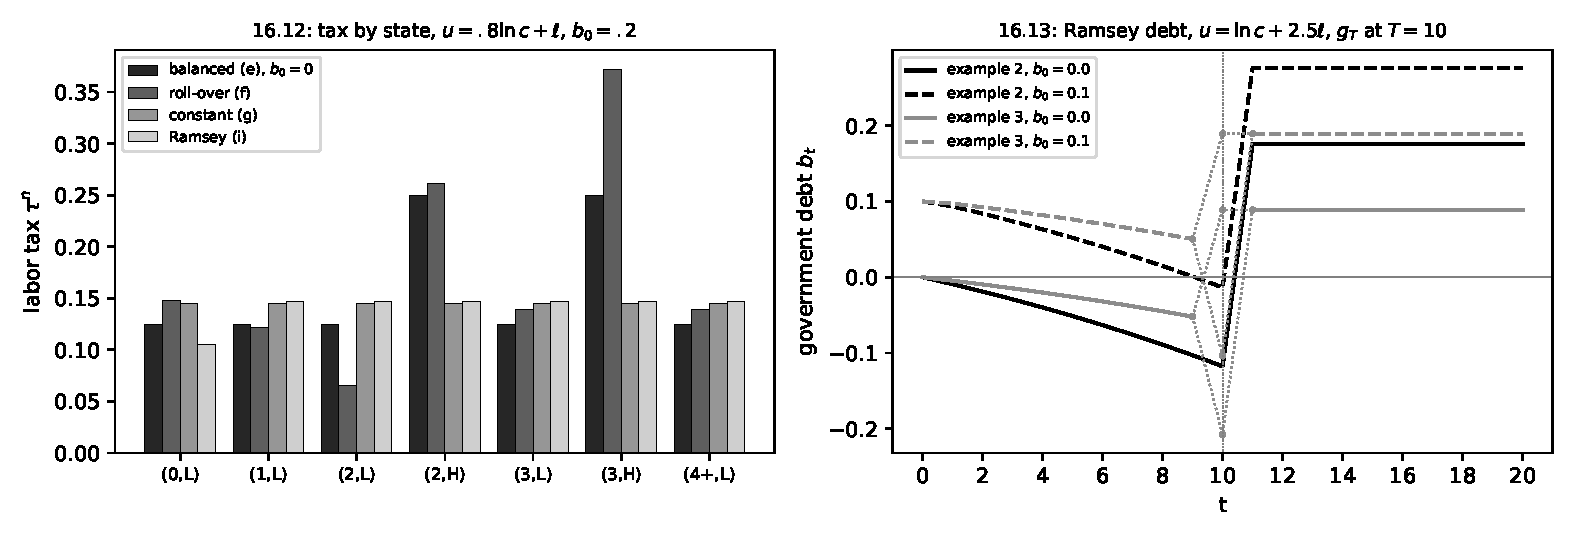
\includegraphics[width=\textwidth]{figures/ch16_01.pdf}\\
{\small Figure S16.1.  Left: labor tax by state in Exercise 16.12 under the balanced-budget ($b_0=0$), roll-over, constant-tax and Ramsey policies ($b_0=.2$).  Right:
Ramsey debt paths in examples 2 and 3 of Exercise 16.13 for $b_0=0$ and $b_0=.1$.  In example 3 the dotted lines fan out to the two date-$T$ states and merge again at
$T+1$.}
\end{center}
\end{ex}

%%---------------------------------------------------------------------------
\begin{ex}{16.13}{Positive initial debt}
\emph{General case.}  For $t\ge1$ the Ramsey allocation still solves (16.12.4), so it remains a time-invariant function of $g_t$, now evaluated at a larger $\Phi$.
More debt requires more revenue, so taxes are higher at all $t\ge1$.  Only the date-0 condition (16.12.5) changes.  Write it as $D(c_0,g_0)=\Phi b_0(u_{cc}-u_{c\ell})$,
where $D(c,g)$ is the left minus the right side of (16.12.4).  Suppose $u_{c\ell}\ge0$ and that $D$ decreases in $c$ (the second-order condition).  Then the right side is
negative, so $c_0>\hat c(g_0)$, the allocation that (16.12.4) prescribes for $g_0$.  Since $u_\ell/u_c$ increases with $c$ along $c+g=1-\ell$, the date-0 tax is below
the tax the plan levies whenever $g_t=g_0$.  As in Section 16.13.4, the planner raises the price $p_0=\beta u_c(1)/u_c(0)$ at which it sells its debt at $t=0$, i.e.\ it
lowers the interest rate on the debt it rolls over.

\emph{Illustration.}  Take $u=\ln c+\kappa\ell$ with $\kappa=2.5$ and $\beta=.95$, and put the spike in examples 2 and 3 at $T=10$ ($g_T=.3$, or $.3$ with probability $.5$).
Then (16.13.1) gives $1/\bar c=(1+\Phi)\kappa$ for every $t\ge1$ \emph{whatever $g_t$ is}.  So for $t\ge1$ consumption and the tax rate $\bar\tau=1-\kappa\bar c
=\Phi/(1+\Phi)$ are constant, including at $T$, and labor $n_t=\bar c+g_t$ absorbs the spike.  The date-0 values solve $(1+\Phi)\kappa c_0^2-c_0-\Phi b_0=0$, and $\Phi$ comes
from $\sum\beta^tE[1-\kappa(c_t+g_t)]=b_0/c_0$.  For $t\ge1$ Arrow prices are $\beta\times$probabilities, and debt is the present value of future surpluses,
$b_t=\bar\tau\bar c/(1-\beta)-(1-\bar\tau)E_t\sum_{j\ge t}\beta^{j-t}g_j$.
\begin{center}
\begin{tabular}{lccccccc}
\toprule
example & $b_0$ & $\Phi$ & $\bar\tau$ ($t\ge1$) & $\tau_0$ & $c_0$ & $\bar c$ & gross rate $0\to1$\\
\midrule
1: $g_t=.1$                 & 0  & .33333 & .25000 & .25000 & .30000 & .30000 & 1.05263\\
                            & .1 & .36895 & .26951 & .18667 & .32533 & .29220 & 0.94542\\
2: $g_{10}=.3$              & 0  & .02297 & .02245 & .02245 & .39102 & .39102 & 1.05263\\
                            & .1 & .03708 & .03575 & .02657 & .38937 & .38570 & 1.04270\\
3: $g_{10}\in\{0,.3\}$      & 0  & .01135 & .01123 & .01123 & .39551 & .39551 & 1.05263\\
                            & .1 & .02487 & .02427 & .01809 & .39277 & .39029 & 1.04601\\
\bottomrule
\end{tabular}
\end{center}

\emph{Example 1.}  With $b_0=0$ the budget balances every period.  With $b_0=.1$ the tax is lower at $t=0$ than later.  At $t=0$ the government runs a primary deficit of
$.0206$ and sells debt at the price $p_0=\beta c_0/\bar c=1.0577$, a negative net interest rate.  From then on it rolls over the constant debt $b_t=.1140$, paying the
interest $.0057$ out of a constant surplus.  Positive initial debt thus breaks perfect tax smoothing only at $t=0$.

\emph{Example 2.}  With $b_0=0$ the book's pattern holds: $b_t$ falls from $-.0092$ at $t=1$ to $-.1177$ at $t=T$ (the government accumulates claims), and after paying
$g_T$ it owes $.1756$ forever.  With $b_0=.1$ the whole path shifts up.  The government starts as a debtor ($b_1=.0935$) and retires its debt with surpluses
$\bar\tau\bar c=.0138$ that exceed the interest.  It becomes a small net creditor just before $T$ ($b_T=-.0135$), then issues debt to pay $g_T$ and owes $.2758$ forever.
The tax is still perfectly smooth for $t\ge1$ (Figure S16.1, right).

\emph{Example 3.}  Before $T$ debt again falls: with $b_0=0$ from $-.0047$ to $-.0521$ at $T-1$, with $b_0=.1$ from $.0972$ to $.0504$.  At $T-1$ the government buys
Arrow securities that pay off if $g_T=.3$.  The date-$T$ debt is $b_T(.3)=-.2078$ and $b_T(0)=.0888$ when $b_0=0$, and $-.1033$ and $.1894$ when $b_0=.1$.  Afterwards it
equals the second number in both states.  The insurance position $b_T(0)-b_T(.3)=(1-\bar\tau)g_T$ ($.2966$ and $.2927$) hardly depends on $b_0$.  Positive initial debt
changes the level of debt, the level of taxes and the date-0 interest-rate manipulation, but not the way the government insures against the spending shock.
\end{ex}

%% ===========================================================================
%% Chapter 17. Self-Insurance
%% ===========================================================================
\solchapter{17}{Self-Insurance}

\begin{center}
\begin{minipage}{0.86\textwidth}
\small
Solutions to all 5 exercises of Chapter 17 of Ljungqvist and Sargent, \emph{Recursive Macroeconomic Theory} (4th edition, 2018).
Numerical examples and checks come from \texttt{code/ch17.py}.
\end{minipage}
\end{center}

\bigskip
\hrule
\bigskip

Throughout, $(1+r)\beta=1$, so with $b_t$ the debt due at $t$ the Euler equation is $u'(c_t)\ge E_tu'(c_{t+1})$, with equality when the borrowing constraint does not bind.

%%---------------------------------------------------------------------------
\begin{ex}{17.1}{Deterministic endowments and borrowing limits}
Solving the budget constraint forward with $b_0=0$ and $\beta=(1+r)^{-1}$ gives the present-value constraint $\sum_t\beta^tc_t\le\sum_t\beta^t\lambda^t=1/(1-\beta\lambda)$.  Ignoring
borrowing constraints, the Euler equation $u'(c_t)=u'(c_{t+1})$ makes consumption constant at
\[
  \bar c=\frac{1-\beta}{1-\beta\lambda},
\]
and the implied debt is the present value of future surpluses, $b_t=\sum_{s\ge t}\beta^{s-t}(y_s-\bar c)=\frac{\lambda^t-1}{1-\beta\lambda}$.

\textbf{(a)}  $\lambda<1$: $b_t=(\lambda^t-1)/(1-\beta\lambda)\le0$ for all $t$.  The unconstrained plan never borrows (the consumer saves early, while income is high), so the no-borrowing
constraint is slack and the optimum is
\[
  c_t=\frac{1-\beta}{1-\beta\lambda},\qquad b_{t+1}=\frac{\lambda^{t+1}-1}{1-\beta\lambda}\le0 .
\]

\textbf{(b)}  $\lambda>1$: now $\bar c>1=y_0$, and the unconstrained plan would borrow.  With $b_{t+1}\le0$, the optimum is $c_t=y_t=\lambda^t$ and $b_{t+1}=0$ for all $t$.  \emph{Proof}: this plan is feasible,
and the Kuhn--Tucker conditions hold with multipliers $\mu_t=u'(c_t)-u'(c_{t+1})=u'(\lambda^t)-u'(\lambda^{t+1})>0$ on the constraints $b_{t+1}\le0$.  The consumer would like to borrow against rising
income every period but cannot.  Saving would move resources from poorer to richer dates, which lowers utility, so consuming the endowment is optimal.  The
problem is concave, so the conditions are sufficient.

\textbf{(c)}  The natural limit is the largest debt that can be repaid with zero consumption forever:
\[
  b_t\le\sum_{j\ge0}\beta^jy_{t+j}=\frac{\lambda^t}{1-\beta\lambda},\qquad t\ge0,
\]
finite because $|\beta\lambda|<1$.  It grows at rate $\lambda$ with the endowment.

\textbf{(d)}  $\lambda<1$: the plan of (a) never borrows, so it satisfies the natural limit and is optimal: $c_t=(1-\beta)/(1-\beta\lambda)$, $b_{t+1}=(\lambda^{t+1}-1)/(1-\beta\lambda)$.

\textbf{(e)}  $\lambda>1$: the unconstrained plan $c_t=(1-\beta)/(1-\beta\lambda)$, $b_{t+1}=(\lambda^{t+1}-1)/(1-\beta\lambda)>0$ satisfies $b_t<\lambda^t/(1-\beta\lambda)$, so the natural limit never binds, and this is the
optimum.  The consumer borrows against his growing income and consumes a constant amount, the annuity value of lifetime income.  Comparing (b) and (e): the ad hoc
constraint matters only when the consumer wants to borrow, i.e.\ when income grows.
\end{ex}

%%---------------------------------------------------------------------------
\begin{ex}{17.2}{Two draws, then permanence}
\textbf{(a)}  From $y_0\in\{1,2\}$ the tree branches once, at $t=1$, into $y_1=2$ (probability $\pi$) or $y_1=1$ (probability $1-\pi$).  After that each branch is a straight line:
$y_t=y_1$ for all $t\ge1$.  All uncertainty is resolved at $t=1$.

\textbf{(b)}  Let $s=a_0-c_0\ge0$ be saving at $t=0$.  From $t=1$ on there is no risk and $(1+r)\beta=1$, so the consumer keeps consumption constant and never needs to borrow.  Wealth at $t=1$ is
$(1+r)s+y_1$, and he consumes its annuity value, $c_t=y_1+(1-\beta)(1+r)s=y_1+rs$ for $t\ge1$, holding $s$ in assets forever.  Using $\beta r/(1-\beta)=1$, the date-0 problem is
\[
  \max_{0\le s\le2}\;\ln(2-s)+\frac\beta{1-\beta}E\ln(y_1+rs),\qquad\text{with FOC}\qquad \frac1{2-s}=\frac\pi{2+rs}+\frac{1-\pi}{1+rs}.
\]
At $s=0$ the right side, $1-\pi/2$, exceeds the left side, $\frac12$, so saving is strictly positive.  Clearing fractions gives a quadratic, whose positive root is
\[
  s=\frac{-(r+2-\pi)+\sqrt{(r+2-\pi)^2+8r(1+r)(1-\pi)}}{2r(1+r)} .
\]
The plan is $c_0=2-s$ and $c_t=y_1+rs$ for $t\ge1$, with lending $s$ at every date.  For example, $r=.05$, $\pi=.5$ gives $s=0.632$, $c_0=1.368$ and $c_t=y_1+0.032$.  The consumer saves
a third of his high initial endowment as a buffer against the possibility that his income drops permanently.

\textbf{(c)}  With $y_0=1$, at $s=0$ the marginal utility of consumption is $1$, while the marginal value of saving is $E[1/y_1]=1-\pi/2<1$: the consumer would like to borrow.  The
no-borrowing constraint binds, so $s=0$, $c_0=1$ and $c_t=y_1$ for $t\ge1$: he simply consumes his endowment.

\textbf{(d)}  For $t\ge2$ (indeed $t\ge1$), $u'(c_t)=1/c_t$ is constant along each branch:
\[
  y_0=2:\ u'(c_t)=\begin{cases}\frac1{2+rs}&\text{prob. }\pi,\\\frac1{1+rs}&\text{prob. }1-\pi;\end{cases}\qquad
  y_0=1:\ u'(c_t)=\begin{cases}\frac12&\text{prob. }\pi,\\1&\text{prob. }1-\pi.\end{cases}
\]

\textbf{(e)}  With $\beta(1+r)=1$, $u'(c_t)\ge E_tu'(c_{t+1})$, so $\{u'(c_t)\}$ is a nonnegative supermartingale and converges almost surely.  Here it converges immediately, to the random limits in (d).
For $y_0=2$ the Euler equation holds with equality at $t=0$ (a martingale); for $y_0=1$ it holds with strict inequality ($1>1-\pi/2$), a strict supermartingale step caused by the binding
constraint.  Chamberlain and Wilson go further: when income keeps fluctuating, the limit of $u'(c_t)$ must be zero, i.e.\ consumption diverges to $+\infty$.  That step fails here
because the endowment becomes \emph{deterministic} after $t=1$.  With no further risk, constant consumption is compatible with the Euler equation, and the limit is a positive random
variable that depends on $y_1$.  So the result conforms to the convergence theorem, but not to the divergence of consumption, whose hypotheses (perpetual, nondegenerate income risk)
are violated.
\end{ex}

%%---------------------------------------------------------------------------
\begin{ex}{17.3}{Natural borrowing limits in the stochastic savings problem}
\textbf{(a)}  The worst case for repayment is the lowest endowment forever, and it has positive probability over any finite horizon.  Repaying $b_{t+1}$ with $c\equiv0$ requires
$b_{t+1}\le\sum_{j\ge0}(1+r)^{-j}y_1=\frac{(1+r)y_1}{r}$.  So debt must satisfy $(1+r)^{-1}b_{t+1}\le y_1/r$, the present value at $t$ of the minimal income stream from $t+1$ on.  Any larger debt
would, on a path of positive probability, force negative consumption.

\textbf{(b)}  Cash on hand is $a_t=y_t-b_t$: the budget $c_t+b_t=y_t+(1+r)^{-1}b_{t+1}$ gives $a_t-c_t=-(1+r)^{-1}b_{t+1}$ and $a_{t+1}=(1+r)(a_t-c_t)+y_{t+1}$.  Substituting
$b_{t+1}=y_{t+1}-a_{t+1}$ into (a):
\[
  a_{t+1}-y_{t+1}\ge-\frac{(1+r)y_1}{r}\qquad(t\ge0).
\]

\textbf{(c)}  \emph{Step 1: the natural limit never binds.}  If debt reached the limit, the consumer would have to set $c=0$ forever on the path where $y=y_1$ forever, which gives
$u'(0)=\infty$.  So he keeps strictly inside it, and the Euler equation holds with equality: $u'(c_t)=E_tu'(c_{t+1})$.
\emph{Step 2: convergence.}  $\{u'(c_t)\}$ is a positive martingale, so by the martingale convergence theorem $u'(c_t)\to M$ almost surely, for a finite random variable $M\ge0$.
\emph{Step 3: $M=0$.}  Suppose $\Prob(M>0)>0$.  On $\{M>0\}$, $c_t\to\bar c=(u')^{-1}(M)<\infty$.  With i.i.d.\ income the problem is stationary in cash on hand, and optimal consumption is $c_t=h(a_t)$
for a continuous, strictly increasing function $h$ (strict concavity).  So $c_t\to\bar c$ implies $a_t\to\bar a=h^{-1}(\bar c)$.  But $a_{t+1}=(1+r)(a_t-h(a_t))+y_{t+1}$, and the first term
converges while $y_{t+1}$ is an independent, nondegenerate draw each period.  So $a_{t+1}$ cannot converge (by Borel--Cantelli it keeps jumping by at least $y_S-y_1$ infinitely often).  This
contradiction shows $M=0$ almost surely, i.e.\ $u'(c_t)\to0$ and $c_t\to+\infty$.  Intuitively, a consumer who never stops facing risk keeps accumulating precautionary assets,
because the martingale $u'(c_t)$ can only settle down where marginal utility is zero.

\textbf{(d)}  The ad hoc constraint set is contained in the natural one, so the value is lower and, starting from the same position, the ad hoc consumer saves more.  He faces
a real risk of hitting the constraint, an extra precautionary motive.  Along identical endowment histories, the natural-limit consumer consumes more early on,
particularly after bad draws (he can borrow), and accumulates assets more slowly.  In both cases $u'(c_t)$ is a nonnegative supermartingale, and the argument of (c) shows that
consumption diverges to $+\infty$ under either constraint.  As wealth grows, both constraints become irrelevant and the two consumption functions approach each other, but the
paths do not coincide, because the levels of wealth they have accumulated differ.  (Section \bk{17.3} also notes that an ad hoc limit can be represented as a natural limit
for a suitably shifted endowment process.)
\end{ex}

%%---------------------------------------------------------------------------
\begin{ex}{17.4}{Trade?}
Note that the aggregate endowment $y_{1t}+y_{2t}=2y_{10}$ is constant, and each individual endowment is a martingale.

\textbf{(a)}  A competitive equilibrium consists of prices $\{q^0_t(s^t)\}$ for history-contingent claims (with $s^t$ the history of $\epsilon$'s) and allocations $\{c_{it}(s^t)\}$, $i=1,2$, such that: each
household maximizes $E_0\sum\beta^tu(c_{it})$ subject to $\sum_t\sum_{s^t}q^0_t(s^t)c_{it}(s^t)\le\sum_t\sum_{s^t}q^0_t(s^t)y_{it}(s^t)$; and markets clear, $c_{1t}(s^t)+c_{2t}(s^t)=y_{1t}(s^t)+y_{2t}(s^t)$ for all $t$ and $s^t$.

\textbf{(b)}  Maximize $E_0\sum\beta^t[u(c_{1t})+u(c_{2t})]$ subject to $c_{1t}+c_{2t}=2y_{10}$.  With equal weights, equal marginal utilities give $c_{1t}=c_{2t}=y_{10}$ for every history:
perfect risk sharing and constant consumption.

\textbf{(c)}  Take $c_{it}=y_{10}$ and $q^0_t(s^t)=\beta^t\pi_t(s^t)$, the marginal utility $u'(y_{10})$ normalized by $u'(y_{10})$ at $t=0$.  Each household's wealth is
$\sum_t\beta^tE_0y_{it}=y_{10}/(1-\beta)$, since each endowment is a martingale.  At these prices a constant $c$ exhausting wealth is $c=y_{10}$, and the first-order conditions
$\beta^t\pi_tu'(c_{it})=\mu_iq^0_t$ hold with $\mu_i=u'(y_{10})$.  Markets clear, so this is the competitive equilibrium: it implements the equal-weight Pareto allocation
because the two households have equal wealth.

\textbf{(d)}  \emph{The guess is correct.}  Suppose $c_{it}=y_{it}$ and $b_{it}=0$.  Household $i$'s Euler equation is $u'(c_{it})=\beta R_tE_tu'(c_{i,t+1})$.  With quadratic utility and a martingale
endowment,
\[
  u_1-u_2y_{it}=\beta R_t\bigl(u_1-u_2E_ty_{i,t+1}\bigr)=\beta R_t(u_1-u_2y_{it}),
\]
so $R_t=\beta^{-1}$ for \emph{both} households at every date and history (as long as consumption stays below bliss).  Bond demands of zero clear the bond market, the budget
constraints hold with $b_{it}=0$, and the terminal condition holds trivially.  So
\[
  R_t=\beta^{-1},\qquad b_{1t}=b_{2t}=0\quad\text{for all }t .
\]
Although the two endowments are perfectly negatively correlated, and complete markets would insure each household fully, a risk-free bond is useless.  Each household
already sees its income as a random walk and wants consumption to be a random walk: the permanent-income consumer consumes his endowment when all shocks are permanent.
Welfare is lower than under complete markets, since consumption has variance growing linearly with $t$ instead of zero.
\end{ex}

%%---------------------------------------------------------------------------
\begin{ex}{17.5}{Trade??}
\textbf{(a)}  \emph{Guess} $b_{t+1}=0$ and $c_t=y_t$ for all $t$.  The Euler equation $c_t^{-\gamma}=\beta RE_tc_{t+1}^{-\gamma}=E_tc_{t+1}^{-\gamma}$ requires
\[
  E_t\Bigl(\frac{y_{t+1}}{y_t}\Bigr)^{-\gamma}=E\exp\bigl(-\gamma\sigma_y\varepsilon-\gamma\mu\bigr)=\exp\Bigl(-\gamma\mu+\frac{\gamma^2\sigma_y^2}{2}\Bigr)=1,
\]
which holds exactly because $\mu=.5\gamma\sigma_y^2$ (confirmed by quadrature in \texttt{ch17.py}).  The plan is feasible and satisfies the natural limit.  Since $\log y$ has i.i.d.\ Gaussian
increments, future income can fall arbitrarily close to zero, so the natural debt limit is in fact zero debt, and $b_{t+1}=0$ respects it.  The transversality condition holds trivially.
The problem is concave, so these conditions are sufficient:
\[
  c_t=y_t,\qquad b_{t+1}=0\quad\text{for all }t .
\]

\textbf{(b)}  Log income is a random walk, so every income shock is permanent.  Consuming current income is then consuming permanent income, as in Friedman's
hypothesis: a permanent shock changes consumption one for one, and there is no reason to save out of it.  (Compare exercise 17.4 and example 1 of section \bk{2.12.3}.)

\textbf{(c)}  Yes, in the sense that matters.  Expected income grows: $E(y_{t+1}/y_t)=e^{\mu+\sigma_y^2/2}>1$.  A certainty-equivalent consumer facing the same expected income path, with $\beta R=1$,
would want constant consumption and would \emph{borrow} against future growth.  The prudent CRRA consumer ($u'''>0$) instead chooses zero borrowing.  The drift
$\mu=.5\gamma\sigma_y^2$ is exactly the growth rate at which the precautionary motive, which increases with $\gamma$ and $\sigma_y^2$, offsets the desire to borrow against expected growth.  Net saving is zero
because precautionary saving and dissaving against expected income growth cancel.
\end{ex}

%% ===========================================================================
%% Chapter 18. Incomplete Markets Models
%% ===========================================================================
\solchapter{18}{Incomplete Markets Models}

\begin{center}
\begin{minipage}{0.86\textwidth}
\small
Solutions to all 7 exercises of Chapter 18 of Ljungqvist and Sargent, \emph{Recursive Macroeconomic Theory} (4th edition, 2018).  Most of the exercises ask for
Bellman equations and definitions of stationary equilibria.  \texttt{code/ch18.py} (Python instead of the book's Matlab) solves the mobility-cost model of 18.2 with
the book's parameters.  It also computes the Huggett and Bewley equilibria of 18.6 and the welfare comparison asked for there, and it illustrates the algorithms of 18.1
and 18.3.
\end{minipage}
\end{center}

\bigskip
\hrule
\bigskip

%%---------------------------------------------------------------------------
\begin{ex}{18.1}{Random discount factor (Bewley--Krusell--Smith)}
To avoid a clash of notation, write $P^\beta_{ij}$ for the discount-factor chain and $P(s,s')$ for the employment chain, and assume the two chains are independent.
Let $v_i(a,s)\equiv v(\bar\beta_i,a,s)$.  The current $\beta_t$ discounts next period's value, so for $i=1,2,3$
\[
  v_i(a,s)=\max_{-\phi\le a'\le(1+r)a+ws}\Bigl\{u\bigl((1+r)a+ws-a'\bigr)+\bar\beta_i\sum_{j=1}^3P^\beta_{ij}\sum_{s'}P(s,s')\,v_j(a',s')\Bigr\}.
\]
These are three coupled Bellman equations.  Equation $i$ involves all three value functions, weighted by row $i$ of $P^\beta$.  If $\beta$ and $s$ are correlated, replace
$P^\beta_{ij}P(s,s')$ by the joint transition probability of $(\beta,s)$; nothing else changes.  The stacked operator $T(v_1,v_2,v_3)$ satisfies Blackwell's conditions:
it is monotone, and $T(v+c)=Tv+\bar\beta_ic\le Tv+\max_i\bar\beta_i\,c$.  So $T$ is a contraction with modulus $\max_i\bar\beta_i<1$ (for bounded $u$), and the solution is
unique.

\emph{Algorithm.}  (1) Discretize assets on a grid $\mathcal A=\{-\phi=\bar a_1<\dots<\bar a_N\}$ and stack the unknowns into $v_i(\bar a_h,\bar s_k)$, a vector of length
$3Nn$.  (2) Start from any guess, e.g.\ $v_i\equiv0$.  (3) Given $v^{(k)}$, compute the continuation values $W_i(a',s)=\sum_jP^\beta_{ij}\sum_{s'}P(s,s')v^{(k)}_j(a',s')$ for
all $(i,a',s)$.  Then maximize $u((1+r)a+ws-a')+\bar\beta_iW_i(a',s)$ over $a'\in\mathcal A$ to get $v^{(k+1)}$ and the policies $g_i(a,s)$.  (4) Iterate to convergence.
Howard's policy improvement (evaluate a fixed policy by solving a linear system, then improve) speeds this up.  Equivalently, one can iterate on the Euler inequality
$u'(c_i(a,s))\ge\bar\beta_i(1+r)\sum_jP^\beta_{ij}\sum_{s'}P(s,s')u'(c_j(a',s'))$, with equality unless $a'=-\phi$, by the endogenous grid method.  (5) The policies and
the two chains induce a Markov chain on $(\beta,a,s)$.  Its invariant distribution gives the cross-section; in a Bewley--Aiyagari economy one then adjusts $r$ until
average assets equal the supply of the asset.

\emph{Illustration.}  Take $u=-1/c$, $r=.02$, $\bar\beta=(.94,.96,.98)$ with
$P^\beta=\bigl[\begin{smallmatrix}.90&.10&0\\.05&.90&.05\\0&.10&.90\end{smallmatrix}\bigr]$, $s\in\{.3,1\}$ with
$P=\bigl[\begin{smallmatrix}.5&.5\\.05&.95\end{smallmatrix}\bigr]$, $w=1$ and $\phi=0$.  The endogenous grid method solves the three coupled equations in a few seconds.
In the invariant distribution, mean assets are $1.08$, $1.28$ and $1.51$ for the three discount factors, which have population shares $(.25,.5,.25)$.  The most patient
quarter holds $29.3\%$ of wealth.  Persistent heterogeneity in patience is what Krusell and Smith use to fatten the upper tail of the wealth distribution.
\end{ex}

%%---------------------------------------------------------------------------
\begin{ex}{18.2}{Mobility costs (Bertola)}
\textbf{(a)}  The state is $(A,w)$, with $w$ the wage of the current job this period.  Staying gives income $RA+w$, and next period's wage is drawn from row $w$.  Moving
gives income $RA+w_g-m$, and the new job's next wage is drawn from the good row.  Writing $E_w[v(A',\cdot)]=P(w,w_g)v(A',w_g)+P(w,w_b)v(A',w_b)$,
\begin{align*}
  v(A,w)&=\max\bigl\{v^s(A,w),\ v^m(A)\bigr\},\\
  v^s(A,w)&=\max_{0\le A'\le RA+w}\bigl\{u(RA+w-A')+\beta E_w[v(A',\cdot)]\bigr\},\\
  v^m(A)&=\max_{0\le A'\le RA+w_g-m}\bigl\{u(RA+w_g-m-A')+\beta E_{w_g}[v(A',\cdot)]\bigr\}.
\end{align*}
In the good state, moving gives the same future as staying but $m$ less today, so $v^m(A)<v^s(A,w_g)$ and nobody leaves a good job.  The moving decision matters only for
$w=w_b$, where the worker trades current income ($w_g-m=.5$ instead of $w_b=1$) for better wage prospects ($p=.8$ instead of $.2$ chance of $w_g$ next period).

\textbf{(b)}  We use value iteration on 601 grid points in $[0,3]$ (418 iterations to a tolerance of $10^{-10}$); see Figure S18.1.  Selected decisions:
\begin{center}
\begin{tabular}{lccc}
\toprule
$A$ & $A'$, $c$ (good wage) & move? (bad wage) & $A'$, $c$ (bad wage)\\
\midrule
0     & .200, 1.200 & no  & .000, 1.000\\
.50   & .655, 1.255 & no  & .350, 1.160\\
.55   & .700, 1.261 & yes & .000, 1.061\\
1.00  & 1.115, 1.305 & yes & .300, 1.220\\
2.00  & 2.060, 1.380 & yes & 1.225, 1.315\\
\bottomrule
\end{tabular}
\end{center}
The moving rule is a wealth threshold: \emph{a worker in a bad job moves if and only if $A\ge.55$}.  The cost must be paid out of current resources and borrowing is not
allowed.  A poor worker could pay it only by cutting consumption sharply, which is very costly with $\sigma=4$, so poor workers stay in bad jobs.  Wealthier workers use
their assets to smooth the cost and move.  A worker just above the threshold spends all his wealth on the move.  In good jobs workers save, and more so the richer they are.
Below about $A=3.3$ assets rise, a buffer against the bad state and a fund for a future move.  In bad jobs they run assets down.  The upper end of the grid is almost
harmless: on $[0,8]$ the good-state saving rule has its fixed point at $A=3.275$, and every statistic below is unchanged to four decimals.

\textbf{(c)}  Let $\tilde w(A,w)=w_g$ if $w=w_g$ or the worker moves, and $\tilde w=w_b$ otherwise.  The decision rules induce the Markov chain
\[
  \Prob\bigl[(A_{t+1},w_{t+1})=(A',w')\mid(A_t,w_t)=(A,w)\bigr]=\mathbf 1\{A'=g(A,w)\}\,P(\tilde w(A,w),w'),
\]
on the $2\times601$ states.  It has exactly one unit eigenvalue (next largest modulus $.910$), so the invariant distribution exists and is unique.  Its recurrent class
has $1188$ states and covers practically all of $[0,3]$, but the mass above $A=2.5$ is only $.002$.

\textbf{(d)}  Read as a cross-section of many workers, the invariant distribution has mean wealth $.711$ and median $.62$.  The 25th and 90th percentiles are $.20$
and $1.55$, and $13.3\%$ of workers hold no assets.  Only $33.2\%$ of workers are in bad jobs, fewer than the $50\%$ the symmetric wage chain alone would imply, because
$11.2\%$ of all workers (a third of those in bad jobs) move each period.  Wealth and job quality are correlated: bad-job workers are poorer (Figure S18.1, right).  About
30\% of them have zero wealth and are stuck, unable to afford a move, while the rest run down their assets or move.  This is Bewley's point in miniature: with incomplete
markets, the wealth distribution affects aggregate mobility, and poor workers are trapped in bad matches.
\begin{center}
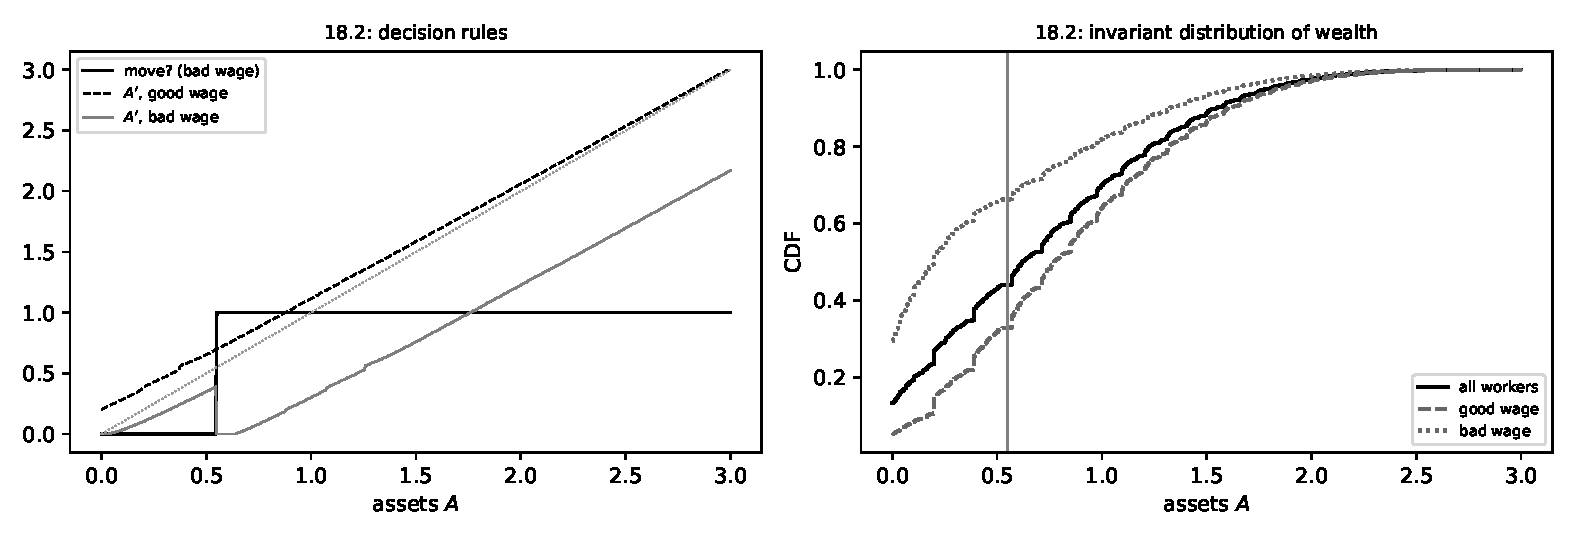
\includegraphics[width=\textwidth]{figures/ch18_02.pdf}\\
{\small Figure S18.1.  Exercise 18.2.  Left: saving rules in the good and bad states and the moving decision (1 = move) in the bad state.  Right: CDF of wealth in the
invariant distribution, overall and by current wage; the vertical line marks the moving threshold $A=.55$.}
\end{center}
\end{ex}

%%---------------------------------------------------------------------------
\begin{ex}{18.3}{Unemployment}
\textbf{(a)}  Use the timing implicit in (b): flows decided at $t$ take effect at $t+1$.  A worker fired at $t$ is unemployed from $t+1$, and an offer accepted at $t$ starts
paying at $t+1$.  Let $V(w)$ be the value of starting a period employed at wage $w$, and $Q$ the value of starting a period unemployed.  Then
\[
  V(w)=w+\beta\bigl[(1-\lambda)V(w)+\lambda Q\bigr],\qquad
  Q=\beta\Bigl[\mu\int\max\{V(w),Q\}\dd F(w)+(1-\mu)Q\Bigr].
\]
So $V(w)=(w+\beta\lambda Q)/(1-\beta(1-\lambda))$ is strictly increasing in $w$, while rejecting yields the constant $Q$.  The optimal policy is therefore to accept iff
$w\ge\bar w$, where $V(\bar w)=Q$, i.e.\ $\bar w=(1-\beta)Q$: the reservation-wage property.  Since $V(w)-Q=(w-\bar w)/(1-\beta(1-\lambda))$, the second equation becomes
\[
  \bar w=\frac{\beta\mu}{1-\beta(1-\lambda)}\int_{\bar w}^\infty(w-\bar w)\dd F(w).
\]
The left side increases and the right side decreases in $\bar w$, so $\bar w(\mu)$ is unique.  It increases with $\mu$: more frequent offers make workers choosier.

\textbf{(b)}  A fraction $\lambda$ of the employed lose their jobs, and a fraction $f(U_t)[1-F(\bar w)]$ of the unemployed find acceptable jobs.  Hence
\[
  U_{t+1}=U_t+\lambda(1-U_t)-f(U_t)\bigl[1-F(\bar w)\bigr]U_t ,
\]
and a stationary rate satisfies $\lambda(1-U)=f(U)[1-F(\bar w)]U$: inflows equal outflows.

\textbf{(c)}  A stationary equilibrium is a pair $(U^*,\bar w^*)$ such that (i) $\bar w^*=\bar w(f(U^*))$ is the optimal reservation wage of a worker who takes
$\mu=f(U^*)$ as given, and (ii) $\lambda(1-U^*)=f(U^*)[1-F(\bar w^*)]U^*$.

\textbf{(d)}  Define $H(U)=f(U)\bigl[1-F(\bar w(f(U)))\bigr]U-\lambda(1-U)$ on $[0,1]$.  For each trial $U$, compute $\mu=f(U)$ and solve the reservation-wage equation
of (a) for $\bar w(\mu)$ by bisection, since its right side is monotone.  Then look for zeros of $H$ by scanning a grid and bisecting on sign changes; several
equilibria are possible, so all sign changes should be found.  Note $H(0)=-\lambda<0$ and $H(1)=0$.  $U=1$ is always a degenerate stationary point: nobody is employed
and no offers arrive.  If $|f'(1)|>\lambda$, then $H<0$ near $0$ and $H>0$ just below $1$ (there $\bar w(0)=0$), so an interior equilibrium exists.  For instance, with
$f(U)=1-U$, $F$ uniform on $[0,1]$, $\beta=.95$ and $\lambda=.05$, the reservation-wage equation is $\bar w=9.7436\,\mu(1-\bar w)^2/2$.  The unique interior equilibrium
is $U^*=.1309$, with $\mu=.8691$ and $\bar w^*=.6180$.
\end{ex}

%%---------------------------------------------------------------------------
\begin{ex}{18.4}{Asset insurance}
First, the Bellman equation should include the non-capital income $y$:
\[
  v(k,x)=\max_{0\le k'\le y+\max(x,g)k^\alpha-\tau}\Bigl\{u\bigl(y+\max(x,g)k^\alpha-k'-\tau\bigr)+\beta\sum_{x'}P(x,x')v(k',x')\Bigr\}.
\]
\rmk{The book's Bellman equation omits $y$, which appears in the budget constraint; it is presumably a typo.}
Given $(g,y,\alpha,\beta,P,\bar x_1,\bar x_2)$, a \emph{stationary equilibrium} is a tax $\tau$, a value function $v$, a decision rule $G$ and a distribution $\lambda$ on
$(k,x)$ such that:
\begin{enumerate}
  \item given $\tau$, $v$ solves the Bellman equation and $G(k,x)$ attains the maximum;
  \item $\lambda$ is stationary under the Markov chain induced by $G$ and $P$:
  \[
    \lambda(k',x')=\sum_x\ \sum_{\{k:\,G(k,x)=k'\}}\lambda(k,x)P(x,x');
  \]
  \item the government's budget balances period by period: the per-capita tax equals per-capita insurance payments,
  \[
    \tau=\max(0,g-\bar x_2)\sum_kk^\alpha\lambda(k,\bar x_2)\quad\Bigl(=\nu-Y\Bigr).
  \]
\end{enumerate}
Output $Y$ and the insured return $\nu$ are then implied.  The resource constraint $\bar c+\bar k=y+Y$ holds automatically, since households receive $\nu$, pay $\tau$, and
$\nu-\tau=Y$.  An equilibrium requires $\tau<y$, so that households with little capital can pay the tax.  Computationally one iterates on $\tau$: guess $\tau$, solve the
Bellman equation, compute $\lambda$, update $\tau$ from 3, and repeat.  Insurance ($g>\bar x_2$) raises the return on capital in the bad state, which encourages
investment.  Because it is financed by a lump-sum tax, it also redistributes toward households with more capital in the bad state.
\end{ex}

%%---------------------------------------------------------------------------
\begin{ex}{18.5}{Matching and job quality (Acemoglu and Shimer)}
\textbf{(a)}  Write $\mathcal U(c,h)=(1-\theta)^{-1}(c(\bar h-h)^\eta)^{1-\theta}$.  Let $W_g,W_b$ be the values of holding a good or bad job, and $V_1,V_0$ the values of
being unemployed and eligible or ineligible, all as functions of assets $a$.  Primes denote next period, and $a'=R(a+y-c)\ge0$.  A job found this period starts next
period, and a quit takes effect immediately.  With $j\in\{g,b\}$ the type searched for and $0\le h\le\min(\bar h,1/m_j)$:
\begin{align*}
  W_g(a)&=\max_{c,h}\Bigl\{\mathcal U(c,h)+\beta\bigl[(1-\delta_g)W_g(a')+\delta_gV_1(a')\bigr]\Bigr\},&& y=w_gh(1-\tau),\\
  W_b(a)&=\max\Bigl\{\max_{c,h}\bigl\{\mathcal U(c,h)+\beta\bigl[(1-\delta_b)W_b(a')+\delta_bV_1(a')\bigr]\bigr\},\ V_0(a)\Bigr\},&& y=w_bh(1-\tau),\\
  V_1(a)&=\max_{c,h,j}\Bigl\{\mathcal U(c,h)+\beta\bigl[m_jh\,W_j(a')+(1-m_jh)\bigl((1-\phi)V_1(a')+\phi V_0(a')\bigr)\bigr]\Bigr\},&& y=b,\\
  V_0(a)&=\max_{c,h,j}\Bigl\{\mathcal U(c,h)+\beta\bigl[m_jh\,W_j(a')+(1-m_jh)V_0(a')\bigr]\Bigr\},&& y=0 .
\end{align*}
The second argument of the max in $W_b$ is the quit option.  A good-job worker could also quit, but never gains from it.  The four equations are coupled through the
transitions.  They can be solved jointly by value iteration on a grid for $a$; for each unemployed state the discrete choice of $j$ is made by comparing the two
maximized values.

\textbf{(b)}  A stationary equilibrium is: a tax rate $\tau$; value functions $(W_g,W_b,V_1,V_0)$; decision rules for consumption and hours or search time in every state,
the search direction $j_e(a)$ for $e\in\{1,0\}$ and the quit rule $q(a)$ in bad jobs; and a distribution $\Gamma$ over $(a,e)$, $e\in\{g,b,1,0\}$, such that:
(i) given $\tau$ (and the exogenous $R,w_g,w_b,b,m_g,m_b,\delta_g,\delta_b,\phi$), the value functions solve the Bellman equations and the rules attain them;
(ii) $\Gamma$ is invariant under the Markov process on $(a,e)$ generated by the rules and the exogenous job-finding, separation and expiry probabilities;
(iii) the insurance budget balances,
\[
  b\,\Gamma(\mathbb R_+,1)=\tau\Bigl[w_g\int h_g(a)\,\Gamma(\dd a,g)+w_b\int h_b(a)\,\Gamma(\dd a,b)\Bigr].
\]
Since $R$ is exogenous (a storage technology or a small open economy), there is no asset-market-clearing condition.  Unemployment, the good/bad job mix, output and welfare
are statistics of $\Gamma$.

\textbf{(c)}  Only the bad-job equation and the law of motion change:
\[
  W_b(a)=\max\Bigl\{\max_{c,h}\bigl\{\mathcal U(c,h)+\beta\bigl[(1-\delta_b)\bigl(\delta_{up}W_g(a')+(1-\delta_{up})W_b(a')\bigr)+\delta_bV_1(a')\bigr]\bigr\},\ V_0(a)\Bigr\}.
\]
In the stationary distribution, a fraction $(1-\delta_b)\delta_{up}$ of bad-job workers move to good jobs each period.

\textbf{(d)}  Yes; it would most likely weaken the case for higher benefits without reversing its logic.  In Acemoglu and Shimer, benefits raise productivity because they
let poorly insured workers take the risk of searching for good jobs (low $m_g$) instead of bad ones.  With upgrades, a bad job is a stepping stone: its value $W_b$ now
contains $\delta_{up}W_g$.  The private and social gap between searching for a good job and taking a bad one therefore shrinks.  Part of the composition gain that more
insurance would bring is obtained anyway, through upgrades.  So the marginal productivity gain from raising $b$ falls, while its moral-hazard cost (longer spells, more
time without work) does not, and the net benefit is smaller.  As $\delta_{up}\to1$ the direction of search hardly matters, and benefits would be justified only by
consumption insurance.  Upgrades also make quitting a bad job to search less attractive, which removes one more channel through which benefit design affects job
quality.  The size of these effects depends on $\delta_{up}$ and must be settled by recalibrating the model.
\end{ex}

%%---------------------------------------------------------------------------
\begin{ex}{18.6}{Gluing stationary equilibria}
\textbf{(a)}  Let $A(r)=[-\phi,\infty)$, with $\phi>0$ an ad hoc limit no looser than the natural one.  A Huggett equilibrium is an interest rate $r$, a value function
$v(a,s)$ and policy $g(a,s)$, and a distribution $\Lambda(a,s)$ such that: (i) given $r$, $g$ solves
$v(a,s)=\max_{a'\in A(r)}\{u((1+r)a+ws-a')+\beta\sum_{s'}P(s,s')v(a',s')\}$; (ii) $\Lambda$ is invariant under the chain induced by $g$ and $P$; (iii) the IOU market
clears, $\sum_{a,s}\Lambda(a,s)g(a,s)=0$.  IOUs are in zero net supply, so $Ea(r)=0$.

\textbf{(b)}  For the economy to be in this stationary equilibrium from time 0, the initial draws must reproduce $\Lambda$.  So $F$ must be the marginal CDF of assets
under $\Lambda$, $F(a)=\sum_s\Lambda(\{\tilde a\le a\},s)$.  Moreover, the joint distribution of $(\tilde a(i,0),s_0(i))$ must be $\Lambda$ itself, not just have
marginals $F$ and the invariant distribution of $P$: poor households are disproportionately in low-income states.

\textbf{(c)}  Figure S18.2 (left) draws the curve for Huggett's (1993) parameters: $\sigma=1.5$, $\beta=.99322$ per sixth of a year, $s\in\{1,.1\}$,
$P=\bigl[\begin{smallmatrix}.925&.075\\.5&.5\end{smallmatrix}\bigr]$, $w=1$ and $\phi=2$.  $Ea(r)$ rises with $r$ and diverges as $r\uparrow\rho=1/\beta-1=.0068$.  It
crosses zero at $r_H=-.01307$ per period ($-7.6\%$ a year), so $r_H<0$.  At $r=0$ average assets are $Ea(0)=1.4231>0$.

\textbf{(d)}  This part sets up the experiment; the transfers are chosen in (f).

\textbf{(e)}  With constant $M_0$ and a constant price level $p$, currency earns $r=0$.  Private IOUs must then also pay $r=0$: if they paid more, nobody would hold
currency, and if they paid less, nobody would hold IOUs.  A stationary Bewley equilibrium is a price level $p>0$, a policy $g_B(a,s)$ and a distribution $\Lambda_B(a,s)$
such that: (i) $g_B$ solves the household's problem at $r=0$ with the same limit $A=[-\phi,\infty)$; (ii) $\Lambda_B$ is invariant; (iii) net asset demand equals the real
value of the outside money, $\sum\Lambda_B(a,s)g_B(a,s)=Ea(0)=M_0/p$ (private IOUs net out).  It exists iff $Ea(0)>0$, i.e.\ iff $r_H<0$ (the case in (c)), and then
$p=M_0/Ea(0)$.  $G$ is the marginal CDF of assets under $\Lambda_B$.  By Proposition 1 of Section 18.6, $Ea(0;\phi)=Ea(0;0)-\phi$, so the equilibrium requires
$\phi<Ea(0;0)$ ($=3.42$ here).

\textbf{(f)}  Index consumers by their rank in the Huggett distribution.  Consumer $i$ holds $a_H(i)=F^{-1}(i)$, where $F^{-1}(u)=\inf\{a:F(a)\ge u\}$ and ties at atoms are
broken by $i$.  Let $\tilde F$ be the CDF of time-0 wealth $(1+r_H)a_H$ and set
\[
  \tilde T_{-1}(i)=G^{-1}(i)-\tilde F^{-1}(i)=G^{-1}(i)-(1+r_H)F^{-1}(i).
\]
Then $a_B(i)=(1+r_H)a_H(i)+\tilde T_{-1}(i)=G^{-1}(i)$.  With $i$ uniform on $(0,1)$, $\Prob\{G^{-1}(i)\le a\}=\Prob\{i\le G(a)\}=G(a)$ (the inverse probability
integral, or Smirnov, transform), so post-transfer assets have CDF $G$.  Both quantile functions are nondecreasing, so every consumer keeps his rank.  Aggregate
transfers equal $\int G^{-1}-(1+r_H)\int F^{-1}=M_0/p-0$, which is the government's budget.  In our example the transfers average $1.4231$ and range from $-.026$ to
$3.005$.  They are slightly negative only for the $0.12\%$ poorest.  Those agents are at the debt limit in both equilibria, and $(1+r_H)(-2)=-1.974>-2$.

The overall-rank scheme reproduces the marginal $G$ but not the joint distribution $\Lambda_B$.  In our example $\Prob(s=\text{low}\mid\text{rank})$ differs between the
two equilibria by up to $.33$, so right after the transfers the economy would not yet be in the stationary Bewley equilibrium.  Applying the same construction \emph{within
each employment state}, with $\tilde T(i,s)=G_s^{-1}(u)-\tilde F_s^{-1}(u)$ where $u$ is $i$'s rank among consumers with the same $s$ and $G_s,\tilde F_s$ are conditional
CDFs, maps $\Lambda_H$ exactly into $\Lambda_B$.  This works because both have the same $s$-marginal, the invariant distribution of $P$.  That scheme preserves ranks
within each state, and it is the one to use if the Bewley equilibrium is to start immediately.

\textbf{(g)}  Not necessarily.  Moving to the Bewley equilibrium raises the interest rate from $r_H<0$ to $0$, which helps lenders and hurts borrowers, and it hands out
$M_0/p$ in transfers, which helps almost everybody.  To sort agents: (1) compute both stationary equilibria and their value functions $v_H(a,s)$ at $r_H$ and $v_B(a,s)$
at $r=0$; (2) for each $(i,s)$ compute Huggett wealth and post-transfer Bewley wealth; (3) the agent prefers the Bewley equilibrium iff
$v_B(a_B(i),s)>v_H(a_H(i),s)$.  With CRRA utility the consumption-equivalent gain is $(v_B/v_H)^{1/(1-\sigma)}-1$.  Under the within-state scheme the comparison is exact,
since the economy is in the Bewley equilibrium from time 0 on.  In our example $99.92\%$ of agents prefer the Bewley equilibrium, with gains of up to $2.7\%$ of
consumption.  The exceptions are the $0.64\%$ poorest low-income agents, $0.08\%$ of the population, who sit at the debt limit.  They lose the subsidy that $r_H<0$
gives to debtors and receive a slightly negative transfer, a loss of $0.73\%$ of consumption.  Figure S18.2 (right) plots the gains.  The overall-rank scheme gives
practically the same split ($99.92\%$).
\begin{center}
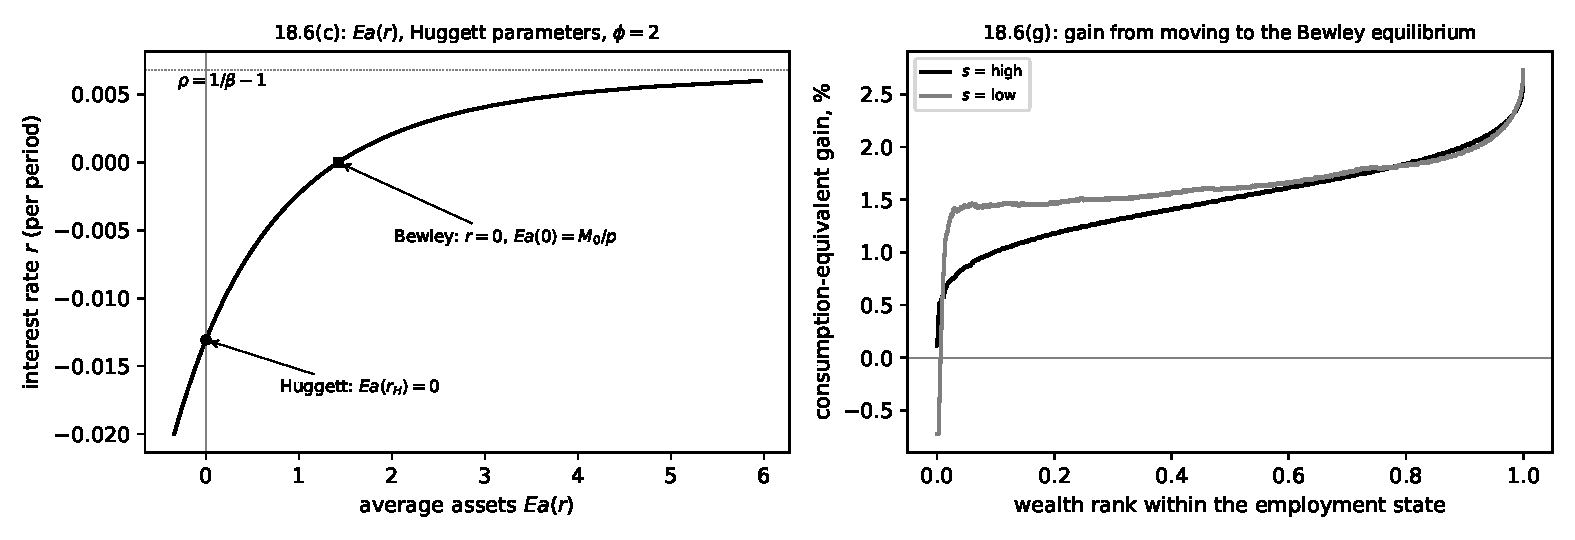
\includegraphics[width=\textwidth]{figures/ch18_06.pdf}\\
{\small Figure S18.2.  Exercise 18.6 with Huggett's parameters.  Left: average assets $Ea(r)$, the Huggett equilibrium $r_H$ and the Bewley equilibrium at $r=0$.  Right:
consumption-equivalent gain from moving to the Bewley equilibrium under rank-preserving transfers within each employment state.}
\end{center}
\end{ex}

%%---------------------------------------------------------------------------
\begin{ex}{18.7}{Real bills}
\exnote{Equation (2) refers to a numbered display of the exercise in the book.}
\textbf{(a)}  Summing $A_{j+1}-A_j=(M_{j+1}-M_j)/p$ over $j=0,\dots,t$ with $A_0=0$ gives $A_{t+1}=(M_{t+1}-M_0)/p$.  The constraint $A_{t+1}\ge0$ means
$M_{t+1}\ge M_0$.

\textbf{(b)}  With $Ea(0)=M_0/p$ and (a), $A_{t+1}+Ea(0)=(M_{t+1}-M_0)/p+M_0/p=M_{t+1}/p$ for every $t$ and every admissible sequence.  At $r=0$ with a constant price level,
currency and IOUs both earn zero, so households are indifferent about the composition of their portfolios.  Their decision rules and $\Lambda_B$ are unchanged.  Their net
asset position, currency plus IOUs held minus IOUs issued, still averages $Ea(0)$.  The extra currency is matched one for one by the IOUs that households have sold to
the monetary authority.

\textbf{(c)}  The price level is pinned down by the time-0 condition $Ea(0)=M_0/p$.  $Ea(0)$ is a property of household behavior at $r=0$ and does not depend on money.
So a larger $M_0$, handed out as in 18.6, raises $p$ in proportion: this is outside money, a net asset of the private sector.  Increases of $M_{t+1}$ above $M_0$ are
backed one for one by private IOUs.  They raise $M_{t+1}/p$ and $A_{t+1}$ equally, leave the net asset supply $M_{t+1}/p-A_{t+1}=M_0/p$ unchanged, and satisfy (2) at the
same $p$.

\textbf{(d)}  $M_0$ is outside money: unbacked and a net asset of households.  $M_{t+1}-M_0$ is inside money: a liability of the monetary authority fully backed by
households' own IOUs, so it is not net wealth.  The real bills doctrine says that money issued against sound short-term private paper is not inflationary.  In this model
it holds exactly: the quantity theory applies to outside money only, and any amount of inside money leaves $p$ unchanged.
\end{ex}

%% ===========================================================================
%% Chapter 19. Dynamic Stackelberg Problems
%% ===========================================================================
\solchapter{19}{Dynamic Stackelberg Problems}

\begin{center}
\begin{minipage}{0.86\textwidth}
\small
Solutions to all 3 exercises of Chapter 19 of Ljungqvist and Sargent, \emph{Recursive Macroeconomic Theory} (4th edition, 2018).
Numerical examples and checks come from \texttt{code/ch19.py}.  Every Stackelberg plan reported below is computed twice, recursively (Riccati equation plus the
initial condition for the forward-looking variable) and by brute force as one large quadratic program, and the two agree to $10^{-13}$.  The script also reproduces the
book's numerical example of Section 19.5.3.
\end{minipage}
\end{center}

\bigskip
\hrule
\bigskip

Notation follows the chapter: $z_t$ are natural state variables, $x_t$ forward-looking variables, $y_t=(z_t',x_t')'$, and the leader minimizes $\sum_t\beta^t(y_t'Ry_t+u_t'Qu_t)$
subject to $y_{t+1}=Ay_t+Bu_t$.  Subproblem 1 gives $v(y)=-y'Py$ with
\[
  P=R+\beta A'PA-\beta^2A'PB(Q+\beta B'PB)^{-1}B'PA,\qquad u_t=-Fy_t,\quad F=\beta(Q+\beta B'PB)^{-1}B'PA,
\]
and subproblem 2 gives $x_0=-P_{22}^{-1}P_{21}z_0$, i.e.\ $\mu_{x0}=0$ for the multiplier $\mu_{xt}=P_{21}z_t+P_{22}x_t$.

%%---------------------------------------------------------------------------
\begin{ex}{19.1}{Optimal monetary policy with commitment}
\exnote{Equations (1)--(3) refer to the numbered displays of the exercise in the book.}
\textbf{(a)}  $m_t-p_t$ is the log of real balances and, under perfect foresight, $p_{t+1}-p_t$ is the expected inflation rate, the opportunity cost of holding money
(the real return on money is $-(p_{t+1}-p_t)$).  Equation (2) is Cagan's demand function: a one-point rise in expected inflation lowers real balances by $\alpha$ percent.
Rearranging (2) gives $(1+\alpha)p_t=m_t+\alpha p_{t+1}$, that is,
\[
  p_t=\frac{1}{1+\alpha}\,m_t+\frac{\alpha}{1+\alpha}\,p_{t+1}=(1-\lambda)m_t+\lambda p_{t+1},\qquad \lambda=\frac{\alpha}{1+\alpha}\in(0,1).
\]
Iterating $T$ times gives $p_t=(1-\lambda)\sum_{j=0}^{T-1}\lambda^jm_{t+j}+\lambda^Tp_{t+T}$.  The homogeneous equation $p_t=\lambda p_{t+1}$ has solutions $c\lambda^{-t}$, so every solution
has the form
\[
  p_t=(1-\lambda)\sum_{j=0}^\infty\lambda^jm_{t+j}+c\,\lambda^{-t}.
\]
The sum converges because $\{m_t\}$ is square summable, hence bounded.  Since $\lambda^{-1}>1$, the term $c\lambda^{-t}$ is an explosive price-level bubble.  The
only square-summable (indeed the only bounded) solution has $c=0$:
\[
  p_t=(1-\lambda)\sum_{j=0}^\infty\lambda^jm_{t+j}=\frac{1-\lambda}{1-\lambda L^{-1}}\,m_t .
\]
The price level is a weighted average of current and future money supplies; the weights $(1-\lambda)\lambda^j$ sum to one.

\textbf{(b)}  Normalize the target log price level to zero.  The authority wants price stability ($p_t^2$) but finds rapid changes in money costly ($u_t^2$).  Since $m_0>0$,
stabilizing prices eventually requires removing money, and doing so quickly is costly.  The authority does not set $p_t$; money holders do, through (2).  By (a),
$p_t=(1-\lambda)\sum_j\lambda^jm_{t+j}$ depends on the whole future path of money.  These equations are \emph{implementability constraints}: a sequence $\{m_t,p_t\}$ can be an
equilibrium outcome only if it satisfies them.  They make the problem a Stackelberg problem.  The authority (the leader) can lower today's price level by promising low
future money supplies, and money holders (the followers) react now to those promises.  Promises about $u_{t+1},u_{t+2},\dots$ thus influence $p_t$ at no adjustment cost
today, but they must be kept later.

\textbf{(c)}  Take the natural state $z_t=m_t$ and the forward-looking variable $x_t=p_t$, with $y_t=(m_t,p_t)'$.  Solving (2) for $p_{t+1}$ gives
$p_{t+1}=\frac{1+\alpha}{\alpha}p_t-\frac1\alpha m_t$, so
\[
  y_{t+1}=Ay_t+Bu_t,\qquad
  A=\begin{bmatrix}1&0\\-1/\alpha&(1+\alpha)/\alpha\end{bmatrix},\quad B=\begin{bmatrix}1\\0\end{bmatrix},
\]
and the criterion is $-\sum_t\beta^t(y_t'Ry_t+u_t^2)$ with $\beta=.95$, $R=\diag(.00001,1)$, $Q=1$.  The second row is the implementability constraint in the form (19.2.6),
$p_t=(1-\lambda)m_t+\lambda p_{t+1}$, with $\phi_0=\lambda\in(0,1)$, so the chapter's Condition A holds.  The problem has two Bellman equations:
\begin{align*}
  \text{subproblem 1:}\quad & v(m,p)=\max_u\Bigl\{-p^2-u^2-.00001m^2+\beta\,v\bigl(m+u,\ \tfrac{1+\alpha}{\alpha}p-\tfrac1\alpha m\bigr)\Bigr\},\\
  \text{subproblem 2:}\quad & w(m_0)=\max_{p_0}v(m_0,p_0).
\end{align*}
Subproblem 1 treats $p$ as if it were inherited; its solution is $v(y)=-y'Py$ and $u=-Fy$ from the Riccati equation above.  Subproblem 2 chooses the initial price level
optimally: $p_0=-P_{22}^{-1}P_{21}m_0$, equivalently $\mu_{p0}=P_{21}m_0+P_{22}p_0=0$.  (The $.00001m^2$ term makes $R$ positive definite, which guarantees a unique
stabilizing solution of the Riccati equation; it has no visible effect on the numbers.)

Why ``dynamic programming squared''?  Money holders' behavior is itself the solution of a dynamic optimization problem, summarized by its Euler equation (2), and the
authority's dynamic program takes that Euler equation as a constraint.  So one dynamic program sits inside another.  As in the book's other uses of the phrase (Chapters 1
and 24), the variable carrying the followers' side of the problem plays a double role.  The price level $p_t$ summarizes money holders' expectations about the future,
so it is forward looking.  It is also, for $t\ge1$, a promise inherited from the past that the authority must keep, so it enters the authority's Bellman equation as a state
variable.  Accordingly the problem needs two Bellman equations with different state vectors: $v(m,p)$ for a continuation leader and $w(m)$ for the leader at time $0$.

\textbf{(d)}  Given $m_0$, a \emph{plan} is a sequence $(\vec u_0,\vec p_0,\vec m_1)=\{u_t,p_t,m_{t+1}\}_{t\ge0}$ that satisfies (1), (2) and the no-bubble condition, i.e.
$p_t=(1-\lambda)\sum_j\lambda^jm_{t+j}$ for all $t$.  Equivalently, a plan is a sequence of possibly history-dependent rules $u_t=\sigma_t(m_0,\dots,m_t)$; with no uncertainty, a
strategy and the sequence it induces carry the same information.  The \emph{continuation} of a plan at date $t$ is its tail $(\vec u_t,\vec p_t,\vec m_{t+1})$.  An optimal
(Stackelberg) plan maximizes (3) over all plans, given $m_0$.

\textbf{(e)}  With $P$ and $F$ from (c),
\[
  p_0=-P_{22}^{-1}P_{21}\,m_0,\qquad u_t=-F\begin{bmatrix}m_t\\p_t\end{bmatrix},\qquad
  \begin{bmatrix}m_{t+1}\\p_{t+1}\end{bmatrix}=(A-BF)\begin{bmatrix}m_t\\p_t\end{bmatrix},\qquad t\ge0 .
\]
The rule is time invariant in $(m_t,p_t)$, but $p_t$ is a linear function of the history $m_0,\dots,m_t$, so $u_t$ is history dependent: it is not a function of $m_t$ alone.
An equivalent representation uses the multiplier $\mu_{pt}=P_{21}m_t+P_{22}p_t$ as the extra state, with initial condition $\mu_{p0}=0$: substituting
$p_t=P_{22}^{-1}(\mu_{pt}-P_{21}m_t)$ into the rule and the law of motion gives a linear system in $(m_t,\mu_{pt})$.

For $\alpha=1$ ($\lambda=.5$), \texttt{ch19.py} gives
\[
  P=\begin{bmatrix}6.79015&-9.44112\\-9.44112&15.06706\end{bmatrix},\qquad u_t=-2.06958\,m_t+2.40759\,p_t,\qquad p_0=.626607\,m_0,
\]
or, in terms of the multiplier,
\[
  u_t=-.56097\,m_t+.15979\,\mu_{pt},\qquad
  \begin{bmatrix}m_{t+1}\\\mu_{p,t+1}\end{bmatrix}=\begin{bmatrix}.43903&.15979\\-.32979&.49138\end{bmatrix}\begin{bmatrix}m_t\\\mu_{pt}\end{bmatrix},\qquad \mu_{p0}=0.
\]
The closed-loop eigenvalues are $.465\pm.228i$, so money and prices converge to zero with damped oscillations.  With $m_0=1$:
\begin{center}
\small
\begin{tabular}{rrrrr}
\toprule
$t$ & $m_t$ & $p_t$ & $u_t$ & $\mu_{pt}$\\
\midrule
0 & 1.00000 & .62661 & $-.56097$ & .00000\\
1 & .43903 & .25321 & $-.29898$ & $-.32979$\\
2 & .14005 & .06739 & $-.12760$ & $-.30685$\\
3 & .01246 & $-.00527$ & $-.03846$ & $-.19697$\\
4 & $-.02600$ & $-.02299$ & $-.00153$ & $-.10090$\\
\bottomrule
\end{tabular}
\end{center}
Along this path $p_t=(1-\lambda)\sum_j\lambda^jm_{t+j}$ holds to machine precision, so the recursive plan respects the implementability constraints.  The authority promises to
overshoot, pushing $m_t$ below zero from $t=4$; that promise lowers the price level at the start.  Figure S19.1 plots the path.

\textbf{(f)}  Disagree.  The plan is time inconsistent: its continuation from $t\ge1$ is not a Stackelberg plan.  At $t=0$ the leader chooses $p_0$ freely (subproblem 2),
which is why $\mu_{p0}=0$.  It also takes into account that promises about $u_1,u_2,\dots$ move $p_0$ through (2).  At $t=1$ the effect of those promises on $p_0$ is sunk.
A leader re-optimizing at $t=1$ would solve subproblem 2 afresh and set $p_1=-P_{22}^{-1}P_{21}m_1$, i.e.\ $\mu_{p1}=0$.  But the continuation of the original plan
delivers the promised $p_1$, with $\mu_{p1}\neq0$.  With $\alpha=1$, $m_0=1$: $m_1=.43903$, the promised $p_1=.25321$ and $\mu_{p1}=-.32979$.  A fresh plan would set
$p_1=.27510$, a looser promise, and would be worth $v=-.168519$, against $-.175737$ for continuing.  The continuation \emph{is} optimal for the \emph{continuation} leader,
who takes the promise $p_1$ as a state (Bellman's principle applies to subproblem 1), but not for a leader who can choose $p_1$ anew.

\textbf{(g)}  A program needs the following steps.
\begin{enumerate}
  \item Set $\lambda=\alpha/(1+\alpha)$, $\beta=.95$, and $A$, $B$, $R=\diag(.00001,1)$, $Q=1$ as in (c).
  \item Iterate $P_{j+1}=R+\beta A'P_jA-\beta^2A'P_jB(Q+\beta B'P_jB)^{-1}B'P_jA$ from $P_0=0$ to convergence; set $F=\beta(Q+\beta B'PB)^{-1}B'PA$.  Check that the
  eigenvalues of $\sqrt\beta(A-BF)$ are inside the unit circle.
  \item Initial price level: $p_0=-(P_{21}/P_{22})\,m_0$.
  \item For $t\ge0$: $u_t=-F_1m_t-F_2p_t$, $m_{t+1}=m_t+u_t$, $p_{t+1}=\frac{1+\alpha}{\alpha}p_t-\frac1\alpha m_t$.
  \item Multipliers $\mu_t=Py_t$ (with $\mu_{p0}=0$); continuation values $v(y_t)=-y_t'Py_t$; value of the plan $w(m_0)=-(P_{11}-P_{12}^2/P_{22})\,m_0^2$.
\end{enumerate}
As a check, \texttt{ch19.py} truncates the problem at $T=400$ ($u_t=0$ afterwards) and minimizes the loss directly over $(u_0,\dots,u_{T-1})$, with $p_t$ given by the
forward solution of (a).  This is a single linear system, and it reproduces the $u_t$ and the loss of the recursive solution to $10^{-13}$.  Table 19.1 reports results for
several $\alpha$.  The larger $\alpha$ is, the more the price level depends on expected future money, and the larger the gain from commitment over the Markov
perfect policy of Exercise 19.2.
\begin{center}
\small
\begin{tabular}{rccccccc}
\toprule
 & \multicolumn{4}{c}{commitment (19.1)} & \multicolumn{3}{c}{Markov perfect (19.2)}\\
\cmidrule(lr){2-5}\cmidrule(lr){6-8}
$\alpha$ & $F_1$ & $F_2$ & $p_0/m_0$ & loss$/m_0^2$ & $g$ & $h$ & loss$/m_0^2$\\
\midrule
0.5 & 3.27025 & $-3.48755$ & .76303 & 1.11784 & $-.61053$ & .76613 & 1.12129\\
1 & 2.06958 & $-2.40759$ & .62661 & 0.87428 & $-.56763$ & .63791 & 0.88659\\
2 & 1.33920 & $-1.80755$ & .48033 & 0.63110 & $-.48938$ & .50537 & 0.65784\\
5 & 0.75667 & $-1.36766$ & .31553 & 0.37773 & $-.36111$ & .35644 & 0.42053\\
\bottomrule
\end{tabular}\\[2pt]
{\small Table 19.1.  Commitment versus Markov perfect policy ($\beta=.95$).  Losses are $-w(m_0)/m_0^2$.}
\end{center}
\begin{center}
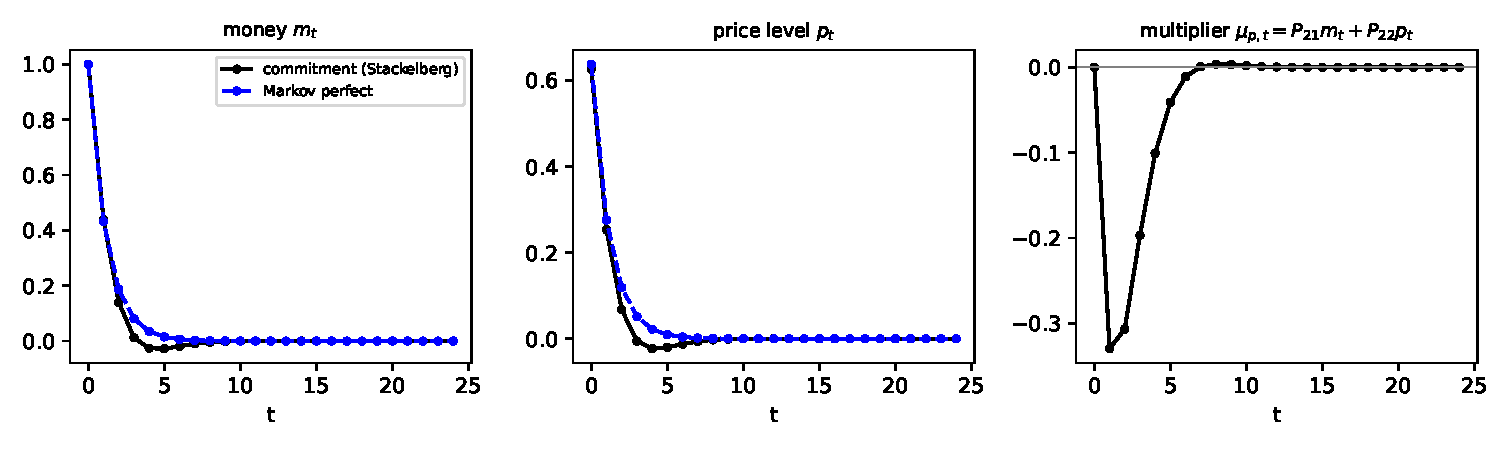
\includegraphics[width=0.95\textwidth]{figures/ch19_01.pdf}\\
{\small Figure S19.1.  $\alpha=1$, $m_0=1$: the Stackelberg plan (solid) and the Markov perfect equilibrium of Exercise 19.2 (dashed).  The multiplier $\mu_{pt}$ starts at zero
and then turns negative: the promises made at $t=0$ bind later.}
\end{center}
\end{ex}

%%---------------------------------------------------------------------------
\begin{ex}{19.2}{Markov perfect policy makers}
\exnote{Equations (2) and (3) refer to the numbered displays of the exercise in the book.}
\textbf{(a)}  If $m_{t+1}=(1+g)m_t$ and $p=hm$, then
$(1-\lambda)m_t+\lambda p_{t+1}=\bigl[(1-\lambda)+\lambda(1+g)h\bigr]m_t$, which equals $hm_t$ if and only if $h\bigl(1-\lambda(1+g)\bigr)=1-\lambda$, i.e.\ $h=(1-\lambda)/(1-\lambda(1+g))$.
When $|\lambda(1+g)|<1$ this is also the forward (bubble-free) solution of Exercise 19.1(a):
$p_t=(1-\lambda)\sum_j\lambda^j(1+g)^jm_t=hm_t$.  All equilibria below have $g\in(-1,0)$, so this condition holds.

\textbf{(b)}  Along $u=gm$, $p=hm$, money is $m_{t+j}=(1+g)^jm_t$, so
\[
  w(m)=-\frac{h^2+g^2+.00001}{1-\beta(1+g)^2}\,m^2\equiv-W(g)\,m^2,\qquad \text{provided }\beta(1+g)^2<1 .
\]
$w(m)$ is the value, to an authority in office when money is $m$, of a world in which (i) it and every successor set money growth by the same Markov rule $u=gm$, and
(ii) money holders know this rule and price accordingly, $p=hm$, which is the rational-expectations price level given the rule.

\textbf{(c)}  The pricing equation is (2) at $t=0$, $p_0=(1-\lambda)m_0+\lambda p_1$, with $p_1=hm_1=h(m_0+u_0)$.  Money holders see the actual $u_0$ (whatever it is) and expect
every authority from $t=1$ on to follow the rule $g$, which makes $p_1=hm_1$.  So the time-$0$ authority knows that its own action moves $p_0$, through its effect on $m_1$ and hence on
expected $p_1$, with slope $\lambda h$.  Functional equation (3) describes an authority that controls only $u_0$.  It takes as given that successors will use $u=gm$ no matter
what it does, and it cannot commit them.  Its continuation value is therefore $w(m_1)$, the value of the rule $g$ from $m_1$ on, and not the value of an optimal
continuation.

\textbf{(d)}  The right side of (3) is strictly concave in $u_0$:
\[
  -\bigl[\lambda h(m_0+u_0)+(1-\lambda)m_0\bigr]^2-u_0^2-.00001m_0^2-\beta W(g)(m_0+u_0)^2 .
\]
The first-order condition $\lambda h\,p_0+u_0+\beta W(m_0+u_0)=0$ gives $u_0=G(g)\,m_0$ with
\[
  G(g)=-\frac{\lambda^2h^2+\lambda(1-\lambda)h+\beta W}{1+\lambda^2h^2+\beta W},\qquad h=h(g),\ W=W(g).
\]
The book calls the maximizer $gm_0$ as well; in equilibrium the two coincide.  A \emph{Markov perfect equilibrium} is a pair of time-invariant linear rules, $u_t=gm_t$ for policy
and $p_t=hm_t$ for prices, together with the value function $w(m)=-W(g)m^2$, such that:
\begin{enumerate}
  \item given that successors use $g$ and future prices obey $h$, the rule $g$ solves the current authority's problem (3) at every $m$: $G(g)=g$;
  \item $h=(1-\lambda)/(1-\lambda(1+g))$: money holders' pricing satisfies their Euler equation (2), without bubbles, given the policy rule;
  \item $w$ is the value of following the rules, $W=W(g)$.
\end{enumerate}
Timing in period $t$: $m_t$ is inherited; the authority in office chooses $u_t$; money holders, seeing $u_t$ and expecting $p_{t+1}=hm_{t+1}$, set
$p_t=(1-\lambda)m_t+\lambda h(m_t+u_t)$, which equals $hm_t$ in equilibrium; then $m_{t+1}=m_t+u_t$ and the next authority takes office.  Each authority assumes that all
successors use $u=gm$ and that the public prices by $p=hm$ from then on.  Money holders assume that every future authority uses $u=gm$.

\textbf{(e)}  The objects to compute are the numbers $g$, $h$, $W$ (hence the functions $u=gm$, $p=hm$, $w=-Wm^2$).  Algorithm: start from $g_0=0$ (any $g_0\in(-1,0]$ will do).
Given $g_j$, compute $h_j=(1-\lambda)/(1-\lambda(1+g_j))$, then $W_j=(h_j^2+g_j^2+.00001)/(1-\beta(1+g_j)^2)$, then $g_{j+1}=G(g_j)$, and stop when $|g_{j+1}-g_j|<10^{-14}$.
Equivalently, solve $G(g)=g$ by bisection.  At least one fixed point exists, and all of them lie in $(-1,0)$.  For $g\in[-1,0]$, $1-\lambda(1+g)\ge1-\lambda$, so $0<h\le1$.
Then $\lambda(1-\lambda)h<1$, so the numerator of $G$ is positive and smaller than its denominator, and $-1<G(g)<0$.  By continuity $G(g)-g$ changes sign on $[-1,0]$.
Admissible $g>0$ (with $\beta(1+g)^2<1$ and $\lambda(1+g)<1$) give $h>0$ and hence $G(g)<0<g$.  Admissible $g<-1$ give $0<h<1-\lambda$ and hence $G(g)>-1>g$.
For $\alpha=1$, the iteration from $g_0=0$ converges in 17 steps to
\[
  g=-.567631,\qquad h=.637905,\qquad W=.886593,
\]
with $|G'(g)|\approx.11$ at the fixed point, and a scan of $(-1,0]$ finds no other fixed point.  Maximizing the right side of (3) numerically at $m_0=1$, with $W$ taken as given,
returns $u_0=-.56763063=g$ and $v(1)=w(1)$, which confirms the equilibrium.  Table 19.1 compares the Markov perfect equilibrium with commitment.  The loss is always larger
without commitment ($.886593$ against $.874279$ for $\alpha=1$), as it must be: the equilibrium outcome $u_t=gm_t$, $p_t=hm_t$ satisfies all the implementability constraints,
so it is one of the plans available to the committed authority of 19.1.  Figure S19.1 shows that the Markov perfect authority contracts money monotonically.  Unable to
promise future tightening, it gets a higher initial price level ($p_0=.638$ against $.627$).

\textbf{(f)}  Yes.  The equilibrium strategies are time-invariant functions of the natural state $m_t$ only.  From any date $t$ and any $m_t$, on or off the equilibrium path,
the continuation uses the same rules $(g,h)$, and conditions 1--3 of (d) hold there because they hold at every $m$.  So the continuation is a Markov perfect
equilibrium starting from $m_t$.  The equilibrium is time consistent by construction.  Contrast Exercise 19.1(f): commitment gives a better outcome but is time inconsistent.
\end{ex}

%%---------------------------------------------------------------------------
\begin{ex}{19.3}{Duopoly with a Stackelberg leader}
\textbf{(a)}  Firm 2 takes the leader's announced sequence $\{Q_{1t}\}$ and $\{v_t\}$ as given, and chooses $\{Q_{2,t+1}\}_{t\ge0}$, with $Q_{20}$ given, to maximize
\[
  \sum_{t=0}^\infty\beta^t\Bigl\{\bigl(A_0-A_1(Q_{1t}+Q_{2t})+v_t\bigr)Q_{2t}-eQ_{2t}-.5gQ_{2t}^2-.5c(Q_{2,t+1}-Q_{2t})^2\Bigr\}.
\]
Unlike the competitive fringe of Section 19.5, firm 2 is not a price taker: it internalizes the effect of its own output on the price.  $Q_{2,t+1}$ appears in the
adjustment costs of periods $t$ and $t+1$ and in the revenue of period $t+1$.  So the first-order condition is, for $t\ge0$,
\[
  c\,(Q_{2,t+1}-Q_{2t})=\beta\bigl[A_0-e-A_1Q_{1,t+1}-(2A_1+g)Q_{2,t+1}+v_{t+1}\bigr]+\beta c\,(Q_{2,t+2}-Q_{2,t+1}).
\]
In terms of the follower's investment $x_t\equiv Q_{2,t+1}-Q_{2t}$,
\[
  x_t=\beta x_{t+1}+\frac\beta c\bigl[A_0-e-A_1Q_{1,t+1}-(2A_1+g)Q_{2,t+1}+v_{t+1}\bigr].
\]
This is the counterpart of (19.5.5): marginal revenue $p-A_1Q_2$ replaces the price, so $(d,h,A_1)$ there become $(e,g,2A_1)$ here.  Add the transversality condition that
rules out explosive paths.  The objective is strictly concave, so the Euler equations and transversality condition characterize the optimum.

To express the link to firm 1 explicitly, divide by $\beta c$:
\[
  Q_{2,t+2}-\phi\,Q_{2,t+1}+\beta^{-1}Q_{2t}=-\frac1c f_{t+1},\qquad \phi=1+\beta^{-1}+\frac{2A_1+g}{c},\quad f_{t+1}=A_0-e-A_1Q_{1,t+1}+v_{t+1}.
\]
The polynomial $z^2-\phi z+\beta^{-1}$ is positive at $0$ and equals $-(2A_1+g)/c<0$ at $1$.  So its roots are $0<\delta_1<1<\delta_2=1/(\beta\delta_1)$.  Factoring
$(1-\delta_1L)(1-\delta_2L)=-\delta_2L(1-\delta_1L)(1-\delta_2^{-1}L^{-1})$ and solving the unstable root forward gives the stable solution
\[
  Q_{2,t+1}=\delta_1Q_{2t}+\frac{\beta\delta_1}{c}\sum_{j=0}^\infty(\beta\delta_1)^j\bigl[A_0-e-A_1Q_{1,t+1+j}+v_{t+1+j}\bigr].
\]
Firm 2's output today depends on the whole future path of firm 1's output: a higher $Q_{1,t+1+j}$ lowers $Q_{2,t+1}$ with weight $A_1\beta\delta_1(\beta\delta_1)^j/c$.  This is the
channel the leader exploits.  With the parameters used below, $\delta_1=.263901$.

\textbf{(b)}  Firm 1 chooses $\{u_t\}=\{Q_{1,t+1}-Q_{1t}\}$ to maximize $\sum_t\beta^t\{p_tQ_{1t}-C_{1t}\}$ subject to the demand curve, the law of motion of $v_t$, and firm 2's
Euler equations, which are its implementability constraints.  Stack $z_t=(1,v_t,Q_{1t},Q_{2t})'$ and $x_t=Q_{2,t+1}-Q_{2t}$, so $y_t=(z_t',x_t)'$.  As in (19.5.6),
{\small
\[
  \begin{bmatrix}1&0&0&0&0\\0&1&0&0&0\\0&0&1&0&0\\0&0&0&1&0\\A_0-e&1&-A_1&-(2A_1+g)&c\end{bmatrix}y_{t+1}
  =\begin{bmatrix}1&0&0&0&0\\0&\rho&0&0&0\\0&0&1&0&0\\0&0&0&1&1\\0&0&0&0&c/\beta\end{bmatrix}y_t+\begin{bmatrix}0\\0\\1\\0\\0\end{bmatrix}u_t .
\]}%
The last row is firm 2's Euler equation.  Premultiplying by the inverse of the left matrix gives $y_{t+1}=Ay_t+Bu_t$.  Firm 1's profit is $-(y_t'Ry_t+u_t'Qu_t)$ with
{\small
\[
  R=-\begin{bmatrix}0&0&\frac{A_0-e}2&0&0\\0&0&\frac12&0&0\\\frac{A_0-e}2&\frac12&-A_1-\frac g2&-\frac{A_1}2&0\\0&0&-\frac{A_1}2&0&0\\0&0&0&0&0\end{bmatrix},\qquad Q=\frac c2 .
\]}%
Solution: (i) solve the Riccati equation for $P$ and $F$ (subproblem 1); (ii) set $x_0=-P_{22}^{-1}P_{21}z_0$ (subproblem 2); (iii) iterate $u_t=-Fy_t$, $y_{t+1}=(A-BF)y_t$.
Stability of $\sqrt\beta(A-BF)$ ensures that the follower's investment sequence is the forward solution of its Euler equation, so it is firm 2's best response.  As in
the chapter, the plan is time inconsistent, since $\mu_{x0}=0$ but $\mu_{xt}\neq0$ for $t\ge1$.

Numerical example, with the chapter's parameters $(A_0,A_1,\rho,c,e,g,\beta)=(100,1,.8,1,20,.2,.95)$:
\begin{align*}
  u_t&=85.3171+.8172v_t-.9789Q_{1t}-2.4873Q_{2t}-3.3790x_t,\\
  x_0&=18.2562+.1770v_0-.0871Q_{10}-.7103Q_{20}.
\end{align*}
The eigenvalues of $A-BF$ are $1,\ .8\ (=\rho),\ .4386,\ .2639\ (=\delta_1),\ .1923$.  Starting from the static Cournot outputs $Q_{10}=Q_{20}=(A_0-e)/(3A_1+g)=25$ with $v_0=0$,
the leader expands and the follower contracts at once ($x_0=-1.679$):
\begin{center}
\small
\begin{tabular}{rrrrr}
\toprule
$t$ & $Q_{1t}$ & $Q_{2t}$ & $p_t$ & $\mu_{xt}$\\
\midrule
0 & 25.000 & 25.000 & 50.000 & 0.000\\
1 & 29.339 & 23.321 & 47.340 & $-5.022$\\
2 & 31.729 & 22.197 & 46.074 & $-6.687$\\
3 & 32.871 & 21.578 & 45.551 & $-7.288$\\
$\infty$ & 33.803 & 20.999 & 45.198 & $-7.682$\\
\bottomrule
\end{tabular}
\end{center}
Two brute-force checks confirm the plan.  (1) Solving firm 2's own sequence problem (a 300-period quadratic program) against the leader's $\{Q_{1t}\}$ reproduces the $\{Q_{2t}\}$
of the plan to $10^{-14}$.  (2) Writing firm 2's best response as an affine function of the whole path $\{Q_{1t}\}$ and maximizing firm 1's profit over that path directly
reproduces the leader's $\{Q_{1t}\}$ to $10^{-12}$.

The long run is the \emph{static} Stackelberg equilibrium.  Put multiplier $\beta^t\theta_t$ on the follower's Euler equation at $t$.  In a steady state, the leader's first-order
condition for $Q_{2t}$ collapses to $-A_1Q_1-(2A_1+g)\theta=0$, because the adjustment-cost terms $-\beta c-c+c+\beta c$ cancel.  So $\theta=-A_1Q_1/(2A_1+g)$.
The condition for $Q_{1t}$ becomes
\[
  A_0-e-(2A_1+g)Q_1-A_1Q_2+\frac{A_1^2}{2A_1+g}Q_1=0,
\]
which is the first-order condition of a static leader facing the static reaction function $Q_2=(A_0-e-A_1Q_1)/(2A_1+g)$.  With our numbers, $Q_1=43.636/1.2909=33.803$ and
$Q_2=20.999$, exactly the limits in the table.  The limit of $\mu_{xt}$ is nonzero, so the leader keeps honoring its promises forever.  Figure S19.2 plots the paths.

\rmk{In Section 19.5.3 the book prints the large firm's rule as $u_t=[-83.98\ \ -0.78\ \ 0.95\ \ 1.31\ \ 2.07]\,y_t$.  Running the same computation (\texttt{ch19.py})
reproduces these numbers as $F$ in $u_t=-Fy_t$, so the printed vector has the wrong sign: the rule is $u_t=83.98+.78v_t-.95Q_t-1.31q_t-2.07i_t$.  With the printed sign,
$Q_{t+1}=1.95Q_t+\cdots$ would explode.  The book's $x_0$ rule $[31.08\ \ 0.29\ \ -0.15\ \ -0.56]$ is reproduced exactly.}

\textbf{(c)}  Firm 2 would pay at most the difference between its value as a monopolist that owns both plants and its value as a follower:
$\text{WTP}(z_0)=V_M(z_0)-V_F(z_0)$.
\begin{itemize}
  \item \emph{Follower's value.}  Firm 2's profit is a quadratic form $-y_t'R_2y_t$ in the leader's state (the adjustment cost $.5cx_t^2$ is in it because $x_t$ is a state).  Along
  the Stackelberg plan $y_{t+1}=(A-BF)y_t$, so $V_F=-y_0'P_Fy_0$, where $P_F=R_2+\beta(A-BF)'P_F(A-BF)$ (a Lyapunov equation solved by doubling) and
  $y_0=(z_0',\,(-P_{22}^{-1}P_{21}z_0)')'$.
  \item \emph{Monopoly value.}  The merged firm chooses $(u_{1t},u_{2t})$ for the two plants with state $z_t=(1,v_t,Q_{1t},Q_{2t})'$ and no implementability constraint.  This is an
  ordinary LQ problem with $A_M=\diag(1,\rho,1,1)$, $B_M=[0\ 0;0\ 0;1\ 0;0\ 1]$, $Q_M=\frac c2I_2$, and
  $-z'R_Mz=(A_0-e+v)(Q_1+Q_2)-A_1(Q_1+Q_2)^2-\frac g2(Q_1^2+Q_2^2)$.  Its Riccati equation gives $V_M=-z_0'P_Mz_0$.
  \item Firm 1 sells only for at least its leader value $V_L(z_0)=-z_0'(P_{11}-P_{12}P_{22}^{-1}P_{21})z_0$.  A deal exists because $V_M\ge V_L+V_F$: the merged firm could
  replicate the Stackelberg outcome.  Any price in $[V_L,\,V_M-V_F]$ works.
\end{itemize}
From $Q_{10}=Q_{20}=25$, $v_0=0$: $V_L=14{,}648.2$, $V_F=10{,}063.5$ (the Lyapunov equation and direct summation of the simulated profits agree), and $V_M=30{,}298.1$.  So firm 2
would pay up to $V_M-V_F=20{,}234.6$, well above firm 1's reservation value $14{,}648.2$, and merging creates a surplus of $5{,}586.4$.  The monopolist runs each plant at
$(A_0-e)/(4A_1+g)=19.048$ in the long run, and the price rises to $61.90$ (Figure S19.2).  All values are quadratic in $z_0$, so the willingness to pay is
$-z_0'(P_M-P_F^z)z_0$, where $P_F^z$ is $P_F$ restricted to $y_0=[I;\,-P_{22}^{-1}P_{21}]z_0$.  For example, it is $19{,}328.4$ from $Q_{10}=Q_{20}=0$ and $20{,}761.3$
from $(Q_{10},Q_{20},v_0)=(25,25,5)$.
\begin{center}
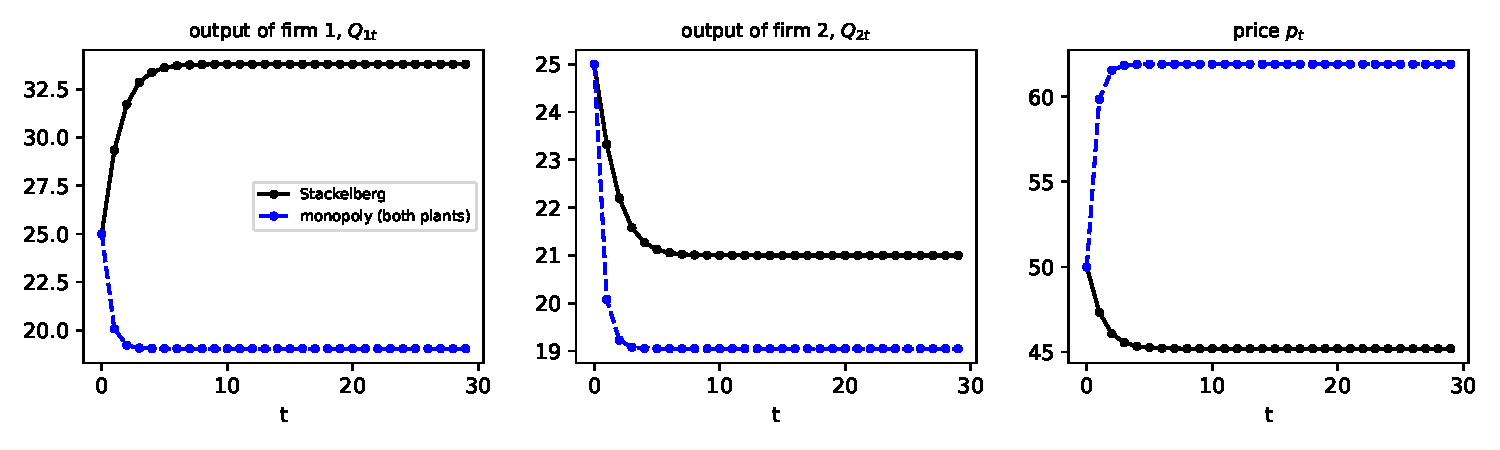
\includegraphics[width=0.95\textwidth]{figures/ch19_03.pdf}\\
{\small Figure S19.2.  Duopoly with firm 1 as Stackelberg leader (solid) versus a monopolist owning both plants (dashed), from $Q_{10}=Q_{20}=25$, $v_0=0$.}
\end{center}
\end{ex}

%% ===========================================================================
%% Chapter 21. Incentives and Insurance
%% ===========================================================================
\solchapter{21}{Incentives and Insurance}

\begin{center}
\begin{minipage}{0.86\textwidth}
\small
Solutions to all 5 exercises of Chapter 21 of Ljungqvist and Sargent, \emph{Recursive Macroeconomic Theory} (4th edition, 2018).  Numbers and figures come from
\texttt{code/ch21.py}, which replaces the book's Matlab programs.  The closed-form moneylender contract is checked to be a fixed point of the Bellman equation.
The Phelan--Townsend version of Exercise 21.4 is solved by value iteration in which each Bellman step is a linear program.
\end{minipage}
\end{center}

\bigskip
\hrule
\bigskip

%%---------------------------------------------------------------------------
\begin{ex}{21.1}{Thomas and Worrall meet Markov}
\textbf{(a)}  In state $(v,i)$ the insurer chooses current consumption $c$ (the transfer is $\tau=c-y_i$) and a promised value $w_j$ for each possible next-period
endowment $y_j$.  Then
\[
  C(v,i)=\min_{c,\{w_j\}}\Bigl\{c-y_i+\beta\sum_{j=1}^IP_{ij}\,C(w_j,j)\Bigr\}\quad\text{subject to}\quad u(c)+\beta\sum_jP_{ij}w_j\ \ge\ v .
\]
The constraint is promise keeping.  It binds at the optimum, because $C$ is increasing in $v$.

\textbf{(b)}  Let $\theta\ge0$ be the multiplier on promise keeping.  The first-order conditions are $1=\theta u'(c)$ and $\beta P_{ij}C_v(w_j,j)=\theta\beta P_{ij}$, and the envelope condition is
$C_v(v,i)=\theta$.  Hence
\[
  C_v(w_j,j)=C_v(v,i)=\frac1{u'(c)}\qquad\text{for all }j:
\]
the insurer equalizes the marginal cost of delivering utility across dates and states.  Since $C_v(w,j)=1/u'(c(w,j))$ at every state, next period's consumption equals
this period's in every state.  So the optimum is full insurance: $c_t=\bar c$ for all $t$ and all histories, with $u(\bar c)=(1-\beta)v$.  Transfers absorb all endowment
risk, $\tau_t=\bar c-y_t$, and promised values stay constant, $v_{t+1}=v_t=v$ in every state.  One can verify directly that
\[
  C(v,i)=\frac{u^{-1}\bigl((1-\beta)v\bigr)}{1-\beta}-Y_i,\qquad Y=(I-\beta P)^{-1}y,
\]
solves the Bellman equation.  Here $Y_i=E[\sum_t\beta^ty_t\given y_0=y_i]$.  With $c=\bar c$ and $w_j=v$, promise keeping holds, and the cost is
$\bar c-y_i+\beta\sum_jP_{ij}(\bar c/(1-\beta)-Y_j)=\bar c/(1-\beta)-Y_i$.  Because $u^{-1}$ is convex, the problem is convex, so the first-order conditions are sufficient.

\textbf{(c)}  In autarky $c_t=y_t$, so $v_a(i)=u(y_i)+\beta\sum_jP_{ij}v_a(j)$, $i=1,\dots,I$; in vector form $v_a=(I-\beta P)^{-1}u(y)$.

\textbf{(d)}  The household must never want to leave.  A promise $v$ made in state $i$ must satisfy $v\ge v_a(i)$, and every continuation promise must satisfy
$w_j\ge v_a(j)$.  So, for $v\ge v_a(i)$,
\[
  C(v,i)=\min_{c,\{w_j\}}\Bigl\{c-y_i+\beta\sum_jP_{ij}C(w_j,j)\Bigr\}\quad\text{s.t.}\quad u(c)+\beta\sum_jP_{ij}w_j\ge v,\quad w_j\ge v_a(j)\ \ \forall j .
\]
With multipliers $\theta$ and $\beta P_{ij}\lambda_j\ge0$, the first-order conditions give $1=\theta u'(c)$ and $C_v(w_j,j)=\theta+\lambda_j$, and the envelope condition gives
$C_v(v,i)=\theta=1/u'(c)$.  Therefore:
\begin{itemize}
  \item if the participation constraint in state $j$ is slack ($\lambda_j=0$), then $C_v(w_j,j)=C_v(v,i)$ and next period's consumption equals this period's;
  \item if it binds ($\lambda_j>0$), then $w_j=v_a(j)$ and $1/u'(c')=C_v(v_a(j),j)>1/u'(c)$, so consumption rises.
\end{itemize}
Consumption never falls.  Let $c^*(j)$ be the consumption the contract gives at state $(v_a(j),j)$.  The constraint binds in state $j$ exactly when $c^*(j)>c_t$, so
\[
  c_{t+1}=\max\{c_t,\ c^*(y_{t+1})\},\qquad v_{t+1}=\begin{cases}\tilde w(c_t,y_{t+1})&\text{if }c_t\ge c^*(y_{t+1}),\\ v_a(y_{t+1})&\text{otherwise,}\end{cases}
\]
where $\tilde w(c,j)$ is the promise that keeps consumption at $c$ in state $j$.  Equivalently, $\tilde w(c,j)=V(c,j)$, where
$V(c,j)=u(c)+\beta\sum_kP_{jk}V(\max\{c,c^*(k)\},k)$ is the value of a contract that pays $c$ until a constraint binds.

This is Kocherlakota's ``amnesia'': whenever a constraint binds, the continuation contract depends only on the current state $y_{t+1}$, not on history.  Consumption is the running
maximum of the thresholds $c^*(y_s)$ (and of $c_0$).  Unlike the i.i.d.\ case of the chapter, promised values need not be monotone.  With constant consumption $c$, the value
$V(c,j)$ depends on the state $j$ because the chance of future binding constraints does, so $v_t$ can fall when the endowment moves to a state in which such constraints are less likely.
\end{ex}

%%---------------------------------------------------------------------------
\begin{ex}{21.2}{Wealth dynamics in the moneylender model}
\textbf{(a)}  With $v_0=v_{aut}$ the contract is the one of Section 21.3.3.  When the highest endowment realized so far is $y_j$, the villager consumes $c_j$ and is promised $w_j$,
where (21.3.25) and the binding participation constraint (21.3.22a) give
\[
  u(c_j)=u(y_j)-\beta\sum_{k\le j}\Pi_k\bigl[u(y_j)-u(y_k)\bigr],\qquad w_j=\frac{u(y_j)+\beta v_{aut}-u(c_j)}{\beta}.
\]
Here $v_{aut}=\sum_s\Pi_su(y_s)/(1-\beta)=-0.173157$ and $E(y)=13.8238$.  The contract is:
\begin{center}
\small
\begin{tabular}{rrrrr@{\hspace{2.2em}}rrrrr}
\toprule
$s$ & $y_s$ & $\Pi_s$ & $c_s$ & $w_s$ & $s$ & $y_s$ & $\Pi_s$ & $c_s$ & $w_s$\\
\midrule
1 & 6 & .07794 & 6.0000 & $-.17316$ & 11 & 16 & .04667 & 13.0334 & $-.14470$\\
2 & 7 & .07404 & 6.9548 & $-.17130$ & 12 & 17 & .04433 & 13.4616 & $-.14223$\\
3 & 8 & .07034 & 7.8564 & $-.16859$ & 13 & 18 & .04212 & 13.8527 & $-.13989$\\
4 & 9 & .06682 & 8.7002 & $-.16550$ & 14 & 19 & .04001 & 14.2100 & $-.13767$\\
5 & 10 & .06348 & 9.4845 & $-.16229$ & 15 & 20 & .03801 & 14.5365 & $-.13557$\\
6 & 11 & .06031 & 10.2096 & $-.15908$ & 16 & 21 & .03611 & 14.8352 & $-.13358$\\
7 & 12 & .05729 & 10.8772 & $-.15595$ & 17 & 22 & .03430 & 15.1086 & $-.13169$\\
8 & 13 & .05443 & 11.4900 & $-.15294$ & 18 & 23 & .03259 & 15.3592 & $-.12990$\\
9 & 14 & .05171 & 12.0512 & $-.15006$ & 19 & 24 & .03096 & 15.5892 & $-.12820$\\
10 & 15 & .04912 & 12.5644 & $-.14731$ & 20 & 25 & .02941 & 15.8005 & $-.12658$\\
\bottomrule
\end{tabular}\\[2pt]
{\small Table 21.1.  The optimal contract with $v_0=v_{aut}$: consumption $c_s$ and promised value $w_s$ after a record endowment $y_s$.}
\end{center}
So $c_t=c_{s(t)}$ and $v_{t+1}=w_{s(t)}$, where $y_{s(t)}=\max\{y_0,\dots,y_t\}$ (21.3.27).  Consumption is constant between record endowments and rises at each new record.
The villager keeps $y_1$ ($c_1=y_1$, $w_1=v_{aut}$) and surrenders $y_s-c_s>0$ in exchange for a higher promise at every other record.

\emph{Checks.}  The two formulas (21.3.22a) and (21.3.24) for $w_j$ agree to $6\times10^{-17}$, and $\sum_s\Pi_s[u(c_s)+\beta w_s]=v_{aut}$.  More importantly, let $P(v)$ be the
closed-form value function of Sections 21.3.3--21.3.5 (with constant consumption $u^{-1}((1-\beta)v)$ for $v\ge w_S$).  The script solves the right side of the Bellman equation
(21.3.4)--(21.3.8) numerically with this $P$: forty choice variables $(c_s,w_s)$, by SLSQP from two starting points.  It does so at ten values of $v$ between $v_{aut}$ and
beyond $w_S$, and gets back $P(v)$ to $8\times10^{-14}$.  So the closed form is a fixed point of the Bellman operator, which is a contraction, and hence it is the value function.

\textbf{(b)}  Profits follow from (21.3.28): $P(w_S)=(E y-c_S)/(1-\beta)$, then backward.  Offering $v_{aut}$ earns
\[
  P(v_{aut})=P(w_1)=2.8405 ,
\]
about 10 percent of the present value of the endowment, $E y/(1-\beta)=27.65$.  (A simulation of 200{,}000 villagers gives $2.841\pm.006$.)  The moneylender captures all the
gains from insurance, because the villager is left at the autarky value.

\textbf{(c)}  By (21.3.38), $F_t(c_j)=\bigl(\sum_{k\le j}\Pi_k\bigr)^{t+1}$, a step function with jumps at the $c_j$ (Figure S21.1, left).  At $t=0$ the distribution mirrors the
endowment distribution, compressed: mass $.078$ at $c_1=6$ and mean consumption $11.23$.  It then shifts right as villagers accumulate record endowments: the mean is
$14.79$ at $t=5$, $15.28$ at $t=10$, and at $t=500$ essentially everyone has had $y_S$ and consumes $c_S=15.80$.  The distribution first fans out and then fans in,
toward complete insurance at the top level.

\textbf{(d)}  Starting from $B_{-1}=0$, the balance obeys $B_t=\beta^{-1}B_{t-1}+E(y)-\sum_jf_{j,t}c_j$ (21.3.40).  With $v_0=v_{aut}$,
\[
  B_0=2.589,\ B_1=6.017,\ B_2=12.05,\ B_5=92.1,\ B_{20}=2.98\times10^6,\ B_{100}=3.60\times10^{30}.
\]
The balance explodes at the rate $\beta^{-1}=2$.  Consistently with (21.3.42), $\beta^{100}(B_{100}+\beta P(w_S))=2.8405=P(v_{aut})$: the moneylender banks a positive
present value of profits, which then compounds.  Eventually each villager is paid $c_S=15.80>E(y)=13.82$, and interest on the balance covers the difference.  (Numerical
note: with $\beta=.5$, iterating (21.3.40) multiplies rounding errors by $2^t$.  So \texttt{ch21.py} uses the equivalent
$B_t=\beta^{-t}P(v_0)-\sum_{s>t}\beta^{s-t}[E(y)-E c_s]$, which agrees with the recursion to $5\times10^{-6}$ for $t<30$.)

\textbf{(e)}  Since $P(w_S)=-3.953<0$, a zero-profit promise exists in $[v_{aut},w_S]$.  Following the recipe of Section 21.3.4: $P(w_{10})=.289>0\ge P(w_{11})=-.138$, so
$k=11$.  The zero-profit condition
$0=\sum_{j<k}\Pi_j(y_j-\tilde c)+\sum_{j\ge k}\Pi_j[y_j-c_j+\beta P(w_j)]$ gives $\tilde c=12.8822$, and (21.3.26) gives
\[
  v_0=-0.145523\in[w_{10},w_{11})=[-0.14731,-0.14470).
\]
The contract pays $\tilde c=12.88$ until the villager's record endowment exceeds $y_{10}$, and $c_j$ afterwards.  A root finder applied to the closed-form $P$ returns the same
$v_0$, and a simulation gives $P(v_0)=-.0001\pm.011$.  The bank balance now converges to $(c_S-E y)/r=1.9767$ (with $r=\beta^{-1}-1=1$): $B_0=.355$, $B_5=1.235$,
$B_{20}=1.768$, $B_{100}=1.967$.  This is the case of the book's Figure 21.3.3.  Even at zero profits the villager gets less than the pooling value
$u(E y)/(1-\beta)=-0.144678$, because the participation constraints still bind.
\begin{center}
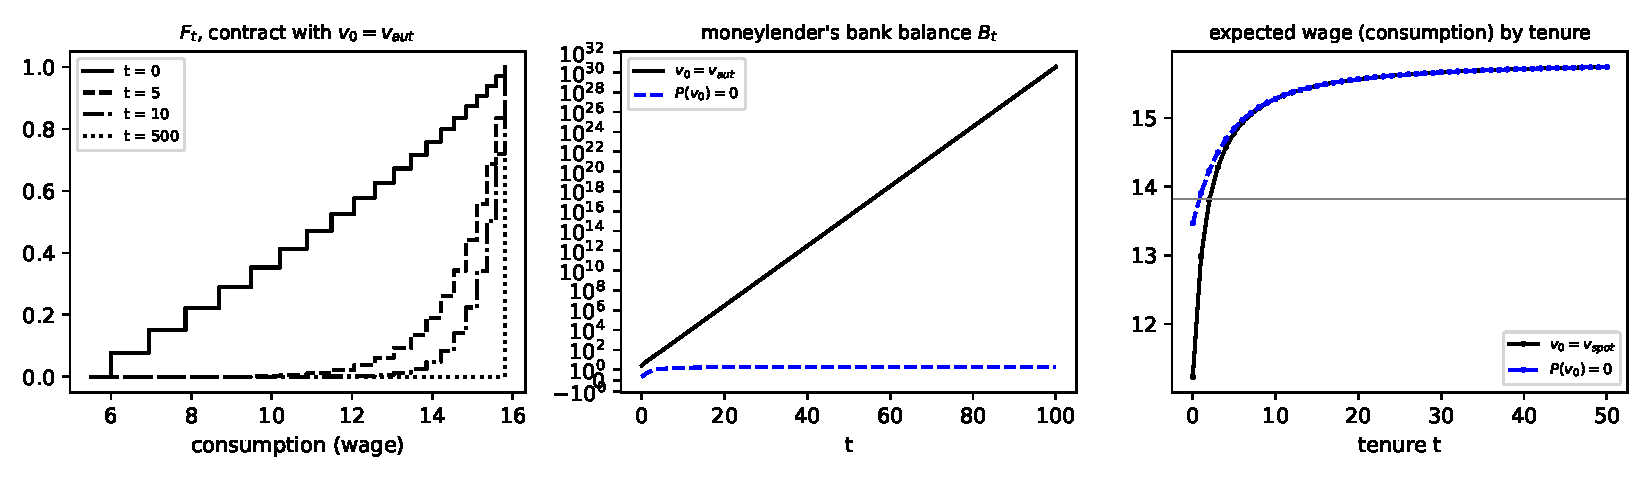
\includegraphics[width=\textwidth]{figures/ch21_02.pdf}\\
{\small Figure S21.1.  Left: $F_t$ for the contract with $v_0=v_{aut}$.  Middle: the moneylender's bank balance (symmetric log scale); it explodes when $v_0=v_{aut}$ and converges
to $1.977$ when $P(v_0)=0$.  Right: expected consumption, i.e.\ the expected wage of Exercise 21.3(d), by tenure.}
\end{center}
\end{ex}

%%---------------------------------------------------------------------------
\begin{ex}{21.3}{Thomas and Worrall (1988)}
This is the moneylender economy of Exercise 21.2 with new labels: productivity $w_t$ is the endowment, the wage $\omega_t$ is consumption, the company is the moneylender, and the
spot market is autarky ($v_{spot}=v_{aut}$).  The parameters are the same, so the numbers are those of Exercise 21.2.
\begin{enumerate}
  \item[(a)] $\omega_t=c_{s(t)}$ and $v_{t+1}=w_{s(t)}$ from Table 21.1, where $s(t)$ indexes the highest productivity the worker has had so far.  The wage never falls: it is constant
  between productivity records and is raised at each record, when the quit constraint binds.  At such a date the worker is paid less than the spot wage ($\omega_t=c_s<w_s$) in
  exchange for a higher promised value.  Wages are rigid downward and backloaded, and the worker is insured against productivity falls.
  \item[(b)] $P(v_{spot})=2.8405$ per worker.
  \item[(c)] $F_t(c_j)=(\sum_{k\le j}\Pi_k)^{t+1}$, as in Figure S21.1 (left).
  \item[(d)] $E\omega_t=\sum_jf_{j,t}c_j$ rises with tenure: $11.23,\ 12.98,\ 13.81$ at $t=0,1,2$, then $14.79$, $15.28$, $15.57$, $15.74$ at $t=5,10,20,50$, and converges to
  $c_S=15.80$ (Figure S21.1, right).  The profile is increasing and concave.  It is steep early, when new records are frequent, and above the mean productivity $13.82$ after about
  two years: senior workers are paid more than they produce.
  \item[(e)] With free entry, competition drives expected profits to zero: $v_0=-0.145523$ as in Exercise 21.2(e).  The entry wage $\tilde c=12.88$ is paid until productivity first
  exceeds $w_{10}=15$.  The expected wage starts higher ($13.47$) and reaches the same limit $c_S$ (dashed line in Figure S21.1, right).
\end{enumerate}
\rmk{The exercise writes the utility function as $(1-\gamma)^{-1}w^{1-\gamma}$; it should be $(1-\gamma)^{-1}\omega^{1-\gamma}$, a function of the wage paid by the company, not of
productivity.}
\end{ex}

%%---------------------------------------------------------------------------
\begin{ex}{21.4}{Thomas and Worrall meet Phelan and Townsend}
\exnote{Equations (4)--(5) refer to the numbered displays of the exercise in the book.}
\textbf{(a)}  The unknowns are the probabilities $x(b,w,y)\equiv\Pi_v(b,w,y)\ge0$.  Given the numbers $P(w)$, the objective $\sum[-b+\beta P(w)]x(b,w,y)$ is linear in $x$.  Promise
keeping is one linear equality whose coefficients $u(y+b)+\beta w$ are numbers once the grids are fixed.  Constraints (4)--(5) amount to the $S$ equalities $\sum_{b,w}x(b,w,y)=\Pi(y)$.
Using $\Pi_v(b,w\given y)=x(b,w,y)/\Pi(y)$, each truth-telling constraint is linear:
\[
  \frac1{\Pi(y)}\sum_{b,w}[u(y+b)+\beta w]\,x(b,w,y)\ \ge\ \frac1{\Pi(\tilde y)}\sum_{b,w}[u(y+b)+\beta w]\,x(b,w,\tilde y) .
\]
So each Bellman step is a linear program with $N_BN_WS$ variables, $1+S$ equalities and $S(S-1)$ inequalities, one program for each promised value $v\in W$.  The lotteries
convexify the planner's problem.  That is Phelan and Townsend's device, and it is what makes linear programming applicable.

\textbf{(b)}  \emph{Implementation.}  Consumption must exceed $a$, so for type $y$ the transfers with $y+b\le a$ are excluded.  In the truth-telling constraints, a lie that would push
consumption to or below $a$ gets utility $-\infty$ (in the code, $-10^4$).  Such lies are never attractive.  $W$ runs from $w_{\min}=-8.3333$ (the value of consuming $y_{\min}$ forever)
to $w_{\max}=-0.4167$.  Each LP has 4{,}775 variables, 11 equalities and 90 inequalities, and \texttt{ch21.py} solves them with HiGHS.
\rmk{As printed, $b_{\min}=1-y_{\max}+.33=-13.67$.  Then $y+b_{\min}<a$ for every endowment, so the lowest grid transfers could never be used.  The statement just before, $B\subset(a-y_S,\bar b]$,
indicates that $b_{\min}=a-y_{\max}+.33=-9.67$ is meant.  We use that value.}

\emph{Which promises can be delivered?}  Most of $W$ cannot be.  To deliver a very low value the contract must give low current utility and low continuation values.  But once
continuation values are at their floor, truth telling forces every type to receive the same transfer: otherwise the types with smaller transfers would report the type with the
largest.  The smallest transfer that keeps the lowest endowment above $a$ is the grid point $b^*=-0.335$.  Hence current utility is at least $E u(y+b^*)$, and the smallest deliverable
value is
\[
  \underline v=\frac{E\,u(y+b^*)}{1-\beta}=-2.4816 .
\]
Value iteration finds this set by itself, in the spirit of the APS operator of Chapter 24.  Starting from $P=0$ on all 25 points, each step finds the LP infeasible at the lowest
remaining promises, because they would need continuation values that were just ruled out.  After 17 steps only the seven grid points $-2.3958,\dots,-0.4167$ remain.  From then on we
iterate on $P$ over the deliverable points.  Value iteration takes 159 steps to reach a step size of $10^{-4}$.  Then one policy-iteration step (an LP improvement step plus an exact
evaluation of the lottery policy, $P=r+\beta MP$) reaches $\max|T(P)-P|=7\times10^{-15}$.  In the final contract promise keeping holds to $4\times10^{-16}$ and truth telling to
$4\times10^{-15}$, and the transition matrix $\Prob(w'\given w)$ has unit row sums.  On the deliverable points,
\[
  P(w)=(45.06,\ 48.65,\ 47.66,\ 44.52,\ 38.57,\ 27.68,\ 4.14)\qquad\text{for }w=-2.40,-2.07,\dots,-0.42 .
\]
With only seven usable points the grid is coarse.  So we also solve the problem with 25 points spanning the deliverable range $[\underline v,w_{\max}]$ (all of them turn out to be
deliverable, and the checks hold to $2\times10^{-10}$).  $P$ is then hump-shaped: it rises from $39.89$ at $\underline v$ to a maximum of $52.82$ near $w=-1.8$ and then falls to $9.93$ at
$w_{\max}$ (Figure S21.2, right).  It increases at the bottom because there all types must get nearly the same transfer, so the planner cannot collect more from high endowments.
Slightly higher promises let it spread continuation values across reports, which relaxes truth telling and raises revenue.  (The planner would never choose to promise values in
that region.)  This spreading is the heart of the contract: at $w_0$ (refined grid) the expected continuation value rises with the reported endowment, from $-2.22$ for $y=6$ to $-1.67$ for $y=15$.
A household that reports a high endowment pays more today and is rewarded with a higher promised value.

\textbf{(c)}  From the joint lottery $\Pi_{w_t}(b_t,w_{t+1},y_t)$,
\[
  \Prob(w_{t+1}=w'\given w_t=w)=\sum_{b\in B,\ y\in Y}\Pi_w(b,w',y),\qquad \Prob(b_t,y_t\given w_t)=\sum_{w'\in W}\Pi_{w_t}(b_t,w',y_t).
\]
Let $p_t(w)=\Prob(w_t=w)$.  Starting from $p_1=\delta_{w_0}$, iterate $p_{t+1}=p_tM$, with $M_{ww'}=\Prob(w'\given w)$.  Consumption is $c_t=y_t+b_t$, so
\[
  \Prob(c_t=c)=\sum_{w}p_t(w)\sum_{(b,w',y):\,y+b=c}\Pi_w(b,w',y),
\]
and $F_t$ is its cumulative sum over the finite support of $y+b$.

\textbf{(d)}  With $w_0$ the grid point closest to $-2$ ($-2.066$ on the book's grid, $-1.965$ on the refined grid):
\begin{center}
\small
\begin{tabular}{rcccc}
\toprule
 & \multicolumn{2}{c}{book's grid} & \multicolumn{2}{c}{refined grid}\\
\cmidrule(lr){2-3}\cmidrule(lr){4-5}
$t$ & mean $c_t$ & std $c_t$ & mean $c_t$ & std $c_t$\\
\midrule
1 & 7.138 & 0.622 & 7.097 & 0.328\\
5 & 7.385 & 0.712 & 7.218 & 0.467\\
10 & 7.548 & 0.741 & 7.321 & 0.535\\
100 & 8.170 & 1.146 & 7.817 & 0.738\\
1000 & 8.246 & 1.206 & 7.945 & 0.809\\
\bottomrule
\end{tabular}
\end{center}
Figure S21.2 plots $F_t$ for $t=1,5,10,100$.  The comparison with Exercise 21.2 is striking.  In the moneylender model, $F_t$ moves right and collapses onto a single point, $c_S$:
eventually every villager has had the highest endowment and is fully insured.  Here the distribution \emph{fans out}.  The dispersion of consumption grows with $t$ and settles at a
nondegenerate invariant distribution, and there is no convergence to full insurance.  To keep households telling the truth, the planner must keep making continuation values
respond to reports, so identical households drift apart and inequality is permanent.  In the Thomas--Worrall model without bounds this spreading never stops: promised values
drift toward $-\infty$ (the immiseration result of Section 21.5.9).  On our grids the minimum transfer bounds consumption below, which keeps promised values in $[\underline v,w_{\max}]$.
Mean consumption rises in this experiment only because $w_0\approx-2$ lies near the bottom of the deliverable set.
\begin{center}
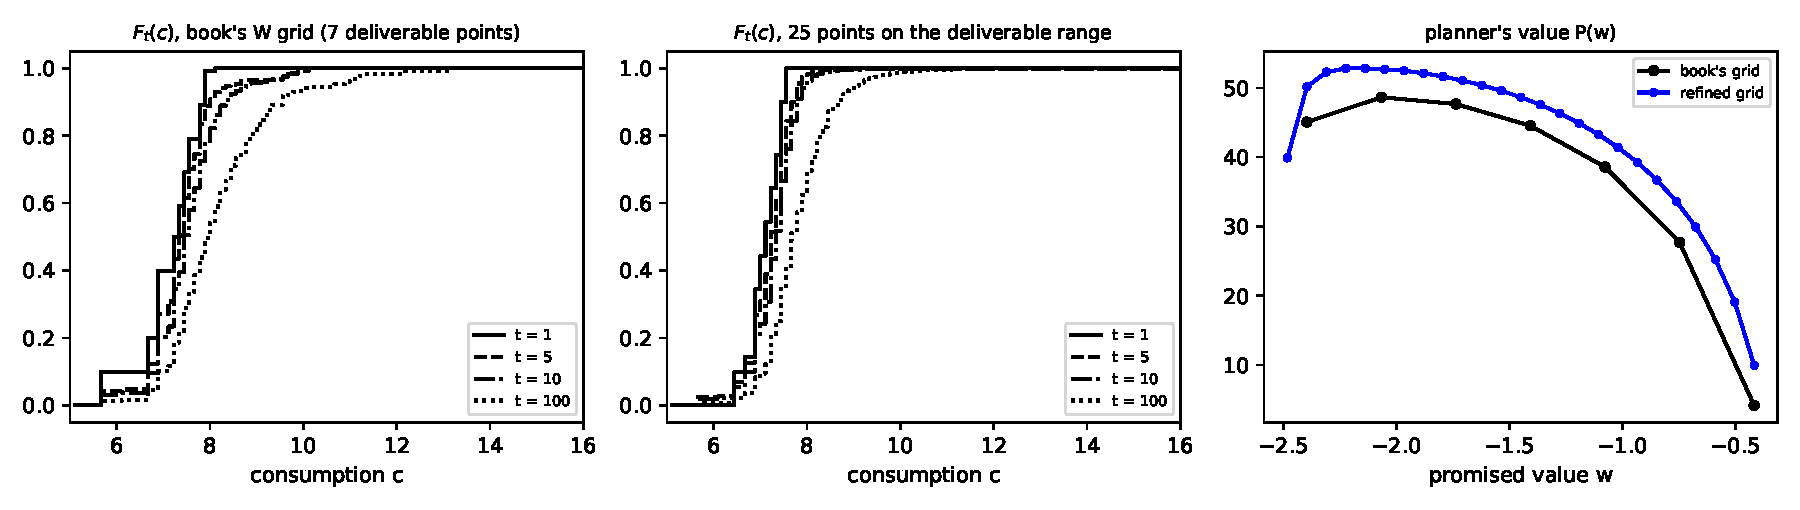
\includegraphics[width=\textwidth]{figures/ch21_04.pdf}\\
{\small Figure S21.2.  Exercise 21.4.  Left and middle: $F_t$ for $w_0\approx-2$ on the book's grid (7 deliverable promised values) and on 25 points spanning the deliverable
range.  Right: the planner's value $P(w)$.}
\end{center}
\end{ex}

%%---------------------------------------------------------------------------
\begin{ex}{21.5}{The IMF}
\textbf{(a)}  Let $v$ be the expected discounted \emph{loss} promised to the country before $g$ is realized, and $P(v)$ the IMF's maximal expected value.  Then
\[
  P(v)=\max_{\{T_s,w_s\}}\sum_{s=1}^S\pi_s\bigl[T_s-g_s+\beta P(w_s)\bigr]
\]
subject to promise keeping, $\sum_s\pi_s[W(T_s)+\beta w_s]\le v$, and the participation constraints
$W(T_s)+\beta w_s\le W(g_s)+\beta v_{aut}$ for $s=1,\dots,S$.  $P$ is increasing: a worse deal for the country is a better one for the IMF.

\textbf{(b)}  With multipliers $\mu$ and $\lambda_s\ge0$, the first-order conditions are $\pi_s=(\mu\pi_s+\lambda_s)W'(T_s)$ and $P'(w_s)=\mu+\lambda_s/\pi_s$, and the envelope
condition is $P'(v)=\mu$.  Hence $W'(T_s)P'(w_s)=1$ in every state.
\begin{itemize}
  \item If the participation constraint is slack, then $w_s=v$ and $W'(T_s)=1/P'(v)$: the tax is the same in all such states (tax smoothing), and the promise is unchanged.
  \item If it binds, then $P'(w_s)>P'(v)$, so $w_s<v$ (a lower future loss) and $T_s$ is lower.  $(T_s,w_s)$ solve $W(T_s)+\beta w_s=W(g_s)+\beta v_{aut}$ and $W'(T_s)P'(w_s)=1$,
  which do not involve $v$ (amnesia).
\end{itemize}
Default is tempting when \emph{spending is low}: financing a low $g_s$ alone costs little, while the contract asks the country to pay for insurance.  So the constraints bind at
low $g$, the mirror image of the high endowments that tempt the villager of Section 21.3.

Starting from $v_{aut}$, the contract works exactly like (21.3.27) with the order of states reversed.  Let $m(t)$ index the \emph{lowest} spending realized so far.  Then
$T_t=T_{m(t)}$ and $v_{t+1}=w_{m(t)}$, where, by the argument that gave (21.3.25),
\[
  W(T_j)=W(g_j)+\beta\sum_{k\ge j}\pi_k\bigl[W(g_k)-W(g_j)\bigr],\qquad w_j=\frac{W(g_j)+\beta v_{aut}-W(T_j)}{\beta}.
\]
To derive the first formula, note that at record $j$ the next period either leaves the record unchanged ($g_k\ge g_j$, loss $A_j\equiv W(g_j)+\beta v_{aut}$) or sets a new record
$k<j$ (loss $A_k$).  So $w_j=A_j\sum_{k\ge j}\pi_k+\sum_{k<j}\pi_kA_k$, and $\sum_k\pi_kA_k=v_{aut}$; substitute into $W(T_j)=A_j-\beta w_j$.  Properties:
$T_S=g_S$ (no transfer when spending is highest); $T_j>g_j$ for $j<S$ (a surplus when a new record low occurs); and
$W(T_j)-W(T_{j-1})=(1-\beta\sum_{k\ge j}\pi_k)[W(g_j)-W(g_{j-1})]>0$, so taxes are lower the lower the record.  Promise keeping holds:
$\sum_s\pi_s[W(T_s)+\beta w_s]=\sum_s\pi_sA_s=v_{aut}$.

\textbf{(c)}  For each country, $T_t$ and $W(T_t)$ are nonincreasing step functions of time.  They are constant while $g_t$ stays above the lowest level seen so far, and they fall
at each new record low.  Once $g_1$ has occurred (which happens eventually with probability one) the tax is constant at $T_1$, with
$W(T_1)=(1-\beta)W(g_1)+\beta EW(g)$.  Surpluses $T_t-g_t$ fluctuate: the IMF lends when $g_t$ is high and collects when it is low.  Across a panel of identical countries the
average surplus at tenure $t$ is $\sum_j\Prob(m(t)=j)T_j-E g$, with $\Prob(m(t)\ge j)=(\sum_{k\ge j}\pi_k)^{t+1}$.  It is positive at $t=0$ (since $T_j\ge g_j$) and declines with tenure
toward $T_1-E g$, whose sign is ambiguous: as $\beta\to0$, $T_1\to g_1<E g$, while as $\beta\to1$, $W(T_1)\to EW(g)\ge W(E g)$.

Yes, there is a cohort effect.  Tax rates, distortions and surpluses depend on the time since a country signed, so at a given calendar date countries that joined earlier have
lower taxes and smaller surpluses.  Panel averages depend on the mix of signing dates.

\emph{Illustration} (\texttt{ch21.py}): $W(T)=T^2$, $g\in\{.1,.2,.3,.4\}$ equally likely, $\beta=.9$.  The record taxes are $T_j=(.2617,.2797,.3252,.4000)$.  The average tax at tenure
$0,1,2,5,10,30$ is $.3167,.2879,.2762,.2657,.2625,.2617$ against $E g=.25$, so the average surplus falls from $.067$ to $.012$.

\textbf{(d)}  Yes: the IMF expects strictly positive profits.  The argument mirrors the book's ``limited obligations'' proof that $P(v_{aut})>0$ (Section 21.3.4), with convexity
of $W$ in place of concavity of $u$.  By convexity, the formula for $W(T_j)$, whose weights sum to one, implies
$T_j\ge(1-\beta q_j)g_j+\beta\sum_{k\ge j}\pi_kg_k$, where $q_j=\sum_{k\ge j}\pi_k$.  The inequality is strict for $j<S$.  Consider the obligation that begins with a record $g_j$
and lasts while $g_t\ge g_j$.  In its first period it earns $T_j-g_j\ge\beta\sum_{k\ge j}\pi_k(g_k-g_j)$.  Afterwards it earns, in expected present value,
\[
  \frac{\beta q_j}{1-\beta q_j}\Bigl(T_j-\frac{\sum_{k\ge j}\pi_kg_k}{q_j}\Bigr)\ \ge\ -\beta\sum_{k\ge j}\pi_k(g_k-g_j).
\]
So each obligation breaks even, and every one with $j<S$ makes a strict profit.  The contract is a collection of such obligations, so $P(v_{aut})>0$.  The country gains
nothing, and the IMF appropriates the whole value of the insurance it provides.  In the illustration $P(v_{aut})=.2243$ (exact, from the recursion analogous to (21.3.28) and
from the distribution of $m(t)$; a simulation gives $.2251\pm.0005$).
\end{ex}

%% ===========================================================================
%% Chapter 22. Equilibrium without Commitment
%% ===========================================================================
\solchapter{22}{Equilibrium without Commitment}

\begin{center}
\begin{minipage}{0.86\textwidth}
\small
Solutions to all 5 exercises of Chapter 22 of Ljungqvist and Sargent, \emph{Recursive Macroeconomic Theory} (4th edition, 2018).  Numbers and figures come from
\texttt{code/ch22.py}.  For Exercise 22.3 the script computes the whole constrained Pareto frontier by value iteration, solving each Bellman step through its concave dual.
This independently confirms the ``amnesia overwhelms memory'' logic of Section 22.10.
\end{minipage}
\end{center}

\bigskip
\hrule
\bigskip

%%---------------------------------------------------------------------------
\begin{ex}{22.1}{A Lagrangian method with two-sided lack of commitment}
\textbf{(a)}  In autarky consumer 1 eats $y_t$ and consumer 2 eats $1-y_t$, so
\[
  v^{aut}_1=\frac{\sum_s\Pi_su(y_s)}{1-\beta},\qquad v^{aut}_2=\frac{\sum_s\Pi_su(1-y_s)}{1-\beta}.
\]
They are equal when the distribution of $y$ is symmetric about $\frac12$ (as in the chapter), but not in general.  After $y_t=y_s$ is observed, the autarky values are
$U_1(y_s)=u(y_s)+\beta v^{aut}_1$ and $U_2(y_s)=u(1-y_s)+\beta v^{aut}_2$.

\textbf{(b)}  Following Marcet and Marimon (Section 21.4), fix a Pareto weight $\alpha\in(0,1)$ and let
$\sum_{j\ge0}\beta^j E_tu(c_i(t+j))$ be consumer $i$'s continuation value.  The planner solves
\[
  \max_{\{c_1(t),c_2(t)\}}E_0\sum_{t=0}^\infty\beta^t\bigl[\alpha u(c_1(t))+(1-\alpha)u(c_2(t))\bigr]
\]
subject to $c_1(t)+c_2(t)\le1$ and, for $i=1,2$ and every history,
$E_t\sum_{j\ge0}\beta^ju(c_i(t+j))\ge U_i(y_t)$.  With multipliers $\beta^t\psi_t$ (feasibility) and $\beta^t\mu_{it}\ge0$ (participation), and using the law of iterated
expectations to collect the terms that multiply each $u(c_i(t))$, the Lagrangian is
\[
  \mathcal L=E_0\sum_{t=0}^\infty\beta^t\Bigl\{\sum_{i=1,2}\bigl[M_{it}u(c_i(t))-\mu_{it}U_i(y_t)\bigr]+\psi_t\bigl(1-c_1(t)-c_2(t)\bigr)\Bigr\},
\]
where
\[
  M_{it}=M_{i,t-1}+\mu_{it},\qquad M_{1,-1}=\alpha,\quad M_{2,-1}=1-\alpha .
\]
The cumulative multipliers $M_{it}$ are ``co-state'' variables.  They make the problem recursive in $(M_{1,t-1},M_{2,t-1},y_t)$, or, by homogeneity, in the single ratio
$x_{t-1}=M_{2,t-1}/M_{1,t-1}$ and $y_t$.

\textbf{(c)}  The first-order conditions for consumption are $M_{1t}u'(c_1(t))=\psi_t=M_{2t}u'(c_2(t))$, with $c_2(t)=1-c_1(t)$.  So
\[
  \frac{u'(c_1(t))}{u'(1-c_1(t))}=x_t\equiv\frac{M_{2t}}{M_{1t}}=\frac{M_{2,t-1}+\mu_{2t}}{M_{1,t-1}+\mu_{1t}} .
\]
The ratio $x_t$ is a time-varying relative Pareto weight, and $c_1(t)=g(x_t)$ with $g$ decreasing.  Consequences:
\begin{enumerate}
  \item \emph{No binding constraint}: $\mu_{1t}=\mu_{2t}=0$, so $x_t=x_{t-1}$ and consumption is unchanged.  The contract insures both consumers fully against the
  endowment realization as long as no participation constraint binds.
  \item \emph{Consumer 1's constraint binds}: $\mu_{1t}>0$ raises consumer 1's weight, so $x_t<x_{t-1}$ and $c_1(t)>c_1(t-1)$.  The multiplier is just large enough that
  the constraint holds with equality.  The value of a contract that restarts from weight $x$ depends only on $x$ (endowments are i.i.d.), so the new weight is a number
  $x^{(1)}(y_t)$ that depends on the current state alone (amnesia).  It is the largest weight consistent with consumer 1's participation.
  \item \emph{Consumer 2's constraint binds}: symmetrically, $x_t=x^{(2)}(y_t)>x_{t-1}$, the smallest weight consistent with consumer 2's participation, and $c_1(t)$ falls.
  \item Only one constraint can bind at a time.  If both did, both consumers would be at their autarky values, which is inefficient when there are gains from trade.
\end{enumerate}
Hence the law of motion of the weight is
\[
  x_t=\min\bigl\{x^{(1)}(y_t),\ \max\{x_{t-1},\ x^{(2)}(y_t)\}\bigr\},
\]
or, in consumption, $c_1(t)=\max\{\underline c(y_t),\min\{c_1(t-1),\bar c(y_t)\}\}$.  Here $[\underline c(y_s),\bar c(y_s)]$ is the interval of consumption levels of consumer 1 that
satisfy both participation constraints in state $y_s$.  The lower end, $c_1(x^{(1)}(y_s))$, makes consumer 1's constraint bind, and the upper end, $c_1(x^{(2)}(y_s))$, makes
consumer 2's bind.  This is exactly (22.4.3).  The thresholds solve the fixed-point conditions $V_1(x^{(1)}(y_s))=U_1(y_s)$ and $V_2(x^{(2)}(y_s))=U_2(y_s)$, where the values of a
contract that starts the period with weight $x$ satisfy
\[
  V_i(x)=u(c_i(x))+\beta\sum_{s'}\Pi_{s'}V_i\bigl(\min\{x^{(1)}(y_{s'}),\max\{x,x^{(2)}(y_{s'})\}\}\bigr).
\]
Properties that follow (Sections 22.4--22.6):
\begin{itemize}
  \item consumption moves only when a constraint binds, and then to the nearest end of the current interval;
  \item the intervals are ordered in $y$ and cannot contain one another, and each contains the endowment;
  \item if all the intervals have a common point $\hat c$, full insurance at $\hat c$ is eventually reached and kept (temporary imperfect risk sharing);
  \item otherwise consumption keeps moving between the lower ends and upper ends forever (permanent imperfect risk sharing).
\end{itemize}
The initial weight $\alpha$ indexes the point on the constrained Pareto frontier, and it matters only until the first binding constraint.
\end{ex}

%%---------------------------------------------------------------------------
\begin{ex}{22.2}{Dixit, Grossman, and Gul (2000)}
\emph{Autarky values.}  Let $\mathbf 1_i(x)=1$ if party $i$ is in power in state $x$.  In autarky the party in power takes everything, so
\[
  A_i(x)=U(\mathbf 1_i(x))+\beta\sum_{x'}P(x,x')A_i(x'),\qquad\text{i.e.}\qquad A_i=(I-\beta P)^{-1}U(\mathbf 1_i).
\]
Here $U(\mathbf 1_i(x))$ is $U(1)$ in power and $U(0)$ out of power.

\emph{Recursive contract.}  The state is the current $x$ and the value $u_0$ promised to party 2 (measured after $x$ is observed).  The contract chooses today's share $y$ of
party 1 and continuation promises $w(x')$ to party 2 for each state tomorrow:
\[
  V(u_0,x)=\max_{y\in[0,1],\ \{w(x')\}}\Bigl\{U(y)+\beta\sum_{x'}P(x,x')\,V\bigl(w(x'),x'\bigr)\Bigr\}
\]
subject to promise keeping, $U(1-y)+\beta\sum_{x'}P(x,x')w(x')\ge u_0$, and the participation constraints in every next-period state,
\[
  w(x')\ge A_2(x'),\qquad V\bigl(w(x'),x'\bigr)\ge A_1(x')\qquad\text{for all }x' .
\]
The current state's participation constraints restrict the domain: $u_0\ge A_2(x)$ and $V(u_0,x)\ge A_1(x)$, i.e.\ $u_0\in[A_2(x),\bar u(x)]$ with $V(\bar u(x),x)=A_1(x)$.
In practice only the party in power can be tempted, because the party out of power gets nothing in autarky today.  Initial promises $u_0$ trace the constrained Pareto frontier
$V(\cdot,x)$.

\emph{Characterization.}  This is Kocherlakota's two-sided model with a Markov state, and the analysis of Exercise 22.1 carries over.  With multiplier $\theta$ on promise
keeping, $U'(y)/U'(1-y)=\theta=-V_u(u_0,x)$.  The share of the party in power stays constant as long as no participation constraint binds.  When the party in power
threatens to take the whole pie, its share jumps to the least generous level that keeps it in, which depends only on the current state (amnesia).  So the contract shares
power ``gradually'': it rewards a party with a larger share when it comes into power only as much as needed to prevent a grab.
\end{ex}

%%---------------------------------------------------------------------------
\begin{ex}{22.3}{A two-state numerical example of social insurance}
Let $u(c)=4c-c^2/2$, so $u(0)=0$, $u(1)=3.5$, $u(2)=6$.  The autarky value is $v_{aut}=\frac{.5[u(2)+u(0)]}{1-\beta}=15$.

\textbf{(a)}  A memoryless contract transfers $\tau\in[0,1]$ from the agent with 2 goods to the agent with 0, so the high agent eats $2-\tau$ and the low agent eats $\tau$.  Every
agent then has the same value before the current draw (22.10.1),
\[
  v(\tau)=\frac{.5[u(2-\tau)+u(\tau)]}{1-\beta}=\frac{3+\tau-\tau^2/2}{1-\beta}.
\]
The low agent never wants to leave, since $u(\tau)\ge u(0)$ and $v(\tau)\ge v_{aut}$.  The high agent stays if
$u(2-\tau)+\beta v(\tau)\ge u(2)+\beta v_{aut}$.  Using $u(2-\tau)=6-2\tau-\tau^2/2$ and multiplying by $1-\beta$, this reduces to
\[
  \tau(3\beta-2)-\tfrac12\tau^2\ \ge\ 0\qquad\Longleftrightarrow\qquad\tau\le2(3\beta-2)=6\beta-4 .
\]
Welfare increases in $\tau$ up to full insurance ($\tau=1$), so the planner picks the largest admissible transfer, $\tau^*=\min\{1,\max\{0,6\beta-4\}\}$.  With $\beta=.8$:
$\tau^*=.8$, so the high agent eats $1.2$ and the low agent $0.8$, with value $v=17.4$ against $v_{aut}=15$ and $17.5$ under full insurance.  Full insurance is not sustainable: at
$\tau=1$ the high agent's constraint fails by $.5$ utils ($18+2-2.5=17.5<18$).

\textbf{(b)}  No.  In this symmetric two-state economy ``amnesia overwhelms memory'' (Section 22.10).  Every period one of the two agents has the high endowment.  If that
agent's constraint binds, amnesia fixes the allocation at $(1.2,0.8)$ whatever the history.  So history can matter only until the first binding constraint.  The formal argument
uses the constrained Pareto frontier $P(v)$ (the best value for agent 2 given $v$ for agent 1, before the endowment is drawn).  $P$ is concave, and at the symmetric point
$\bar v=17.4$ it has a kink with one-sided slopes
\[
  -\frac{u'(0.8)}{u'(1.2)}=-\frac{3.2}{2.8}=-1.143\quad\text{(right)},\qquad -\frac{u'(1.2)}{u'(0.8)}=-0.875\quad\text{(left)}
\]
(Section 22.10.1).  Since $-1$ lies between them it is a supergradient, so $P(v)\le P(\bar v)-(v-\bar v)$, i.e.\ $v+P(v)\le2\bar v=34.8$ for every sustainable
allocation.  The equally weighted optimum is therefore the memoryless contract of (a).  History dependence can move along the frontier, e.g.\ promise $\hat v>\bar v$ to an agent
who has not yet had a low endowment (the frontier extends to $v_{\max}=[u(2)+u(.8)+\beta\bar v]/(2-\beta)=19$), but only at a loss in total welfare.

\emph{Numerical check.}  \texttt{ch22.py} computes the ex ante frontier by value iteration.  It starts from the first-best frontier (an upper bound) and solves each Bellman step
through its Lagrangian dual, $P(v)=\min_{\mu\ge0}[D(\mu)-\mu v]$, which is exact because the step is a concave program.  After 97 iterations the frontier lives on $[15,19]$, as
the theory says.  $\max_v[v+P(v)]=34.80000$ is attained at $v=17.4000$, and the numerical one-sided slopes at $\bar v$ are $-0.864$ and $-1.160$ (finite differences over $.1$;
theory $-.875$, $-1.143$).  Figure S22.1 plots the frontier.
\begin{center}
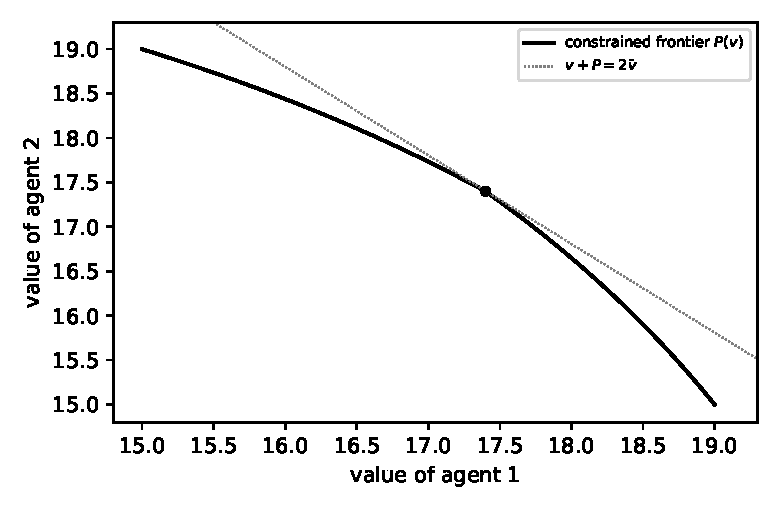
\includegraphics[width=0.55\textwidth]{figures/ch22_03.pdf}\\
{\small Figure S22.1.  Constrained Pareto frontier of Exercise 22.3.  It touches the line $v+P=34.8$ only at the kink $(17.4,17.4)$, the memoryless contract.}
\end{center}

\textbf{(c)}  From (a), $\tau^*(\beta)=\min\{1,\max\{0,6\beta-4\}\}$.  As $\beta$ rises, the future gains from staying in the arrangement grow relative to the one-period gain from
walking away with the high endowment, so more insurance is sustainable.  For $\beta\ge5/6$ the contract gives full insurance ($\tau=1$), and in particular as $\beta\to1$.  As
$\beta$ falls, insurance shrinks, and for $\beta\le2/3$ no transfer is sustainable: the contract collapses to autarky, and in particular as $\beta\to0$.  (\texttt{ch22.py}
confirms the formula at nine values of $\beta$ by solving the participation constraint numerically.)
\end{ex}

%%---------------------------------------------------------------------------
\begin{ex}{22.4}{Kehoe--Levine without risk}
Here $u(c)=-1/(c+5)$ and $u'(c)=(c+5)^{-2}$, with $u(1.5)=-.153846$, $u(1)=-.166667$, $u(.5)=-.181818$.

\textbf{(a)}  Endowments alternate, so
\[
  v_{aut,h}=\frac{u(1.5)+\beta u(.5)}{1-\beta^2}=-0.831391,\qquad v_{aut,\ell}=\frac{u(.5)+\beta u(1.5)}{1-\beta^2}=-0.846931 .
\]

\textbf{(b)}  The aggregate endowment is constant at 2 and preferences are identical.  With $q^0_t=\beta^t$, each household's first-order condition $\beta^tu'(c_{it})=\lambda_iq^0_t$ makes
its consumption constant, and constant consumption clears the market.  So Arrow--Debreu prices are $q^0_t=\beta^t$, the one-period gross interest rate is $1/\beta=1.25$, and each
household consumes the annuity value of its endowment.  Type 1, rich at $t=0$, has wealth
$(1.5+.8\cdot.5)/(1-.64)=5.2778$, so
\[
  c_1=(1-\beta)\cdot5.2778=1.055556,\qquad c_2=0.944444 .
\]

\textbf{(c)}  $v_1^{CE}=u(1.055556)/(1-\beta)=-0.825688$ and $v_2^{CE}=u(0.944444)/(1-\beta)=-0.841121$.

\textbf{(d)}  At every odd date type 2 has the high endowment.  Its continuation value in the competitive allocation is $v_2^{CE}=-0.841121<v_{aut,h}=-0.831391$, so it would
rather renege and eat its endowment.  (At even dates both types prefer the competitive allocation: $-0.825688>-0.831391$ and $-0.841121>-0.846931$.  So the violations occur at
odd dates, not at every $t>0$.)

\textbf{(e)}  Let $A_i(t)$ be household $i$'s autarky value from $t$ on ($v_{aut,h}$ or $v_{aut,\ell}$ according to the parity of $t$).  The planner solves
\[
  \max_{\{c_{1t}\}}\sum_t\beta^tu(c_{1t})\quad\text{s.t.}\quad\sum_t\beta^tu(2-c_{1t})\ge\tilde v_2,\qquad
  \sum_{j\ge0}\beta^ju(c_{i,t+j})\ge A_i(t)\ \ \forall i,t .
\]
Recursively, with the parity $p\in\{\text{even},\text{odd}\}$ and the promise $v_2$ to household 2 as states,
$V(v_2,p)=\max_{c,v_2'}\{u(c)+\beta V(v_2',1-p)\}$ subject to $u(2-c)+\beta v_2'\ge v_2$, $v_2'\ge A_2(1-p)$ and $V(v_2',1-p)\ge A_1(1-p)$.

\textbf{(f)}  In the periodic allocation the household with the high endowment eats $\check c\ge1$ and the other eats $2-\check c$, so
\[
  v_h=\frac{u(\check c)+\beta u(2-\check c)}{1-\beta^2},\qquad v_\ell=\frac{u(2-\check c)+\beta u(\check c)}{1-\beta^2}.
\]
The low household's constraint is slack.  The function $g(\check c)=u(2-\check c)+\beta u(\check c)$ is concave, equals $u(.5)+\beta u(1.5)$ at $\check c=1.5$, and is larger at
$\check c=1$ ($-.3000$ against $-.3049$).  So $g(\check c)>u(.5)+\beta u(1.5)$, i.e.\ $v_\ell>v_{aut,\ell}$, for every $\check c\in[1,1.5)$.  The high household's constraint, $v_h\ge v_{aut,h}$, fails at full smoothing ($\check c=1$ gives
$-0.833333<-0.831391$).  The function $\check c\mapsto u(\check c)+\beta u(2-\check c)$ is concave and equals $u(1.5)+\beta u(.5)$ at $\check c=1.5$.  So the efficient (most
smoothing) choice is its other root:
\[
  \check c=1.168224,\qquad v_h=v_{aut,h}=-0.831391,\qquad v_\ell=-0.836587 .
\]
Figure S22.2 compares the three allocations.  Autarky has large swings, $1.5,.5,\dots$.  Complete markets smooth perfectly, but at levels (1.056 and .944) set by initial wealth.
With enforcement the swings shrink to $1.168,.832$ and the continuation values alternate.  The high-endowment household is held exactly at its autarky value, while the
low-endowment household gets strictly more than autarky.  Under complete markets the continuation values are constant, which is why type 2's constraint fails in the periods
when it is rich.

\textbf{(g)}  Without enforcement constraints $R=1/\beta=1.25$ every period.  With them, the Alvarez--Jermann decentralization prices a one-period bond by the household whose
constraint does not bind next period, the one that is rich today:
\[
  R=\Bigl[\max_i\beta\frac{u'(c_{i,t+1})}{u'(c_{it})}\Bigr]^{-1}=\frac{u'(\check c)}{\beta u'(2-\check c)}=1.117355
\]
at every date (the allocation is periodic).  The rate is lower with enforcement.  The poor household would like to borrow against its high endowment tomorrow, but it cannot
promise to repay, because tomorrow it would default.  Its borrowing is restricted, so the rich household, which wants to save, must be induced by a low interest rate to hold the
limited supply of claims.  Its consumption falls tomorrow, and it values future consumption highly.

\textbf{(h)}  As $\beta$ rises the future matters more, so more smoothing is sustainable and $\check c$ falls.  Full smoothing becomes sustainable when $(1+\beta)u(1)\ge u(1.5)+\beta u(.5)$,
i.e.\ for
\[
  \beta\ \ge\ \beta^*=\frac{u(1.5)-u(1)}{u(1)-u(.5)}=0.846154 .
\]
For $\beta\ge\beta^*$, $\check c=1$ and both economies have $R=1/\beta$.  For $\beta<\beta^*$ the rate with enforcement is lower: for example $1.1593$ against $1.2048$ at $\beta=.83$.
At $\beta^*$ the high household's constraint holds with equality at full smoothing but no longer restricts the allocation (a zero multiplier), and for $\beta>\beta^*$ no
participation constraint binds.  (The competitive allocation of (b) is not the periodic one, but its interest rate is $1/\beta$ at any $\beta$.)
\begin{center}
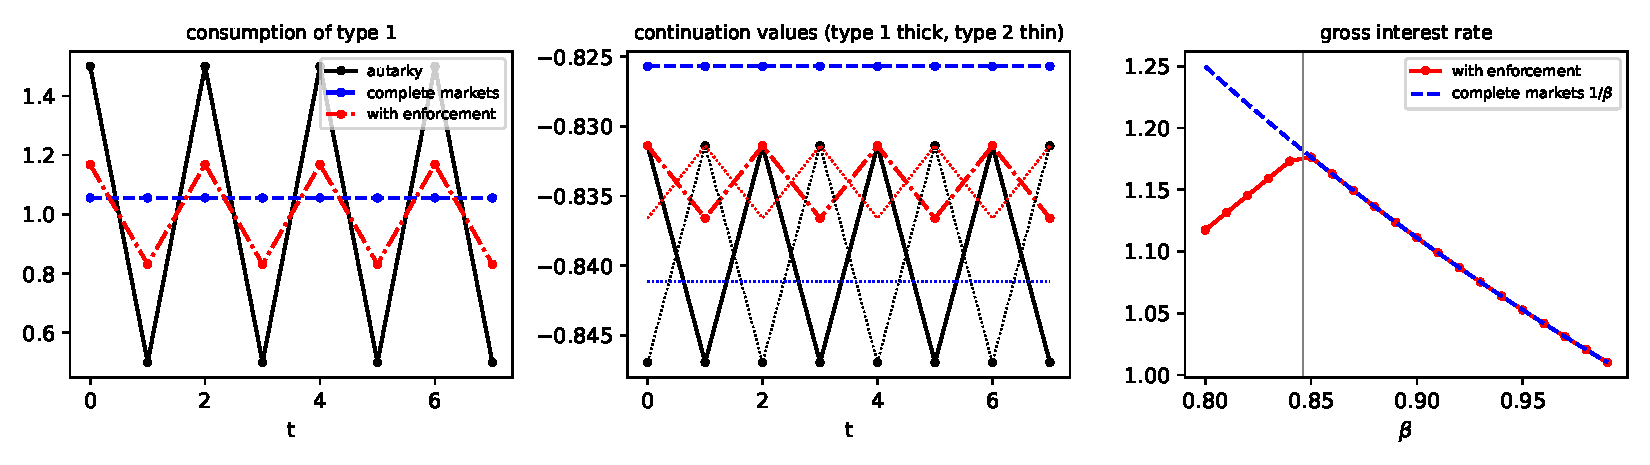
\includegraphics[width=\textwidth]{figures/ch22_04.pdf}\\
{\small Figure S22.2.  Exercise 22.4.  Left: consumption of type 1.  Middle: continuation values (type 1 thick, type 2 thin).  Right: gross interest rates as functions of
$\beta$; they coincide for $\beta\ge\beta^*=.846$.}
\end{center}
\end{ex}

%%---------------------------------------------------------------------------
\begin{ex}{22.5}{The kink}
\textbf{(a)}  The aggregate endowment is always 1.  With equal weights and strictly concave $u$, the planner equates consumption: $c_1=c_2=.5$ at every date and history.

\textbf{(b)}  Let $q^0_t(h^t)=\beta^t\Pi(h^t)$ be the time-0 price of consumption after history $h^t$, where $\Pi(h^t)=.5^{t+1}$.  With constant consumption, each consumer's
first-order conditions $\beta^t\Pi(h^t)u'(c_t(h^t))=\lambda_iq^0_t(h^t)$ hold with $\lambda_i=u'(.5)$.  Each consumer's endowment is worth $\sum_t\beta^tE y_t=.5/(1-\beta)$, which buys
$.5$ per period, so budgets balance and markets clear.  A one-period risk-free bond costs $\sum_{y'}\beta\,.5=\beta$, so its gross return is $R=1/\beta$.

\textbf{(c)}  In autarky each consumer eats its endowment, so $v_{aut}=.5[u(y)+u(1-y)]/(1-\beta)$ ex ante.  After observing the endowment, the autarky value is $u(y)+\beta v_{aut}$ for the
high agent and $u(1-y)+\beta v_{aut}$ for the low agent.  The ex ante problem maximizes consumer 2's expected utility subject to consumer 1 getting at least a given value, feasibility,
and, after every history, each consumer's continuation value being at least its autarky value given its current endowment.

\textbf{(d)}  Use the conditional frontiers of Thomas and Worrall (22.3.1).  With states $s\in\{1,2\}$ ($y_1=1-y$, $y_2=y$) and $x$ consumer 1's promised surplus over autarky in the
current state,
\[
  Q_s(x)=\max_{c,\chi_1,\chi_2}\Bigl\{u(1-c)-u(1-y_s)+\beta\sum_j.5\,Q_j(\chi_j)\Bigr\}
\]
subject to $u(c)-u(y_s)+\beta\sum_j.5\chi_j\ge x$, $\chi_j\ge0$ and $Q_j(\chi_j)\ge0$ for $j=1,2$, with $c\in[0,1]$.  Equivalently, the ex ante frontier $P(v)$ solves
$P(v)=\max\sum_s.5[u(1-c_s)+\beta P(w_s)]$ subject to $\sum_s.5[u(c_s)+\beta w_s]\ge v$ and the four participation constraints
$u(c_s)+\beta w_s\ge u(y_s)+\beta v_{aut}$, $u(1-c_s)+\beta P(w_s)\ge u(1-y_s)+\beta v_{aut}$.

\textbf{(e)}  The Part I allocation gives $u(.5)/(1-\beta)$ forever, and only the high agent's constraint can fail.  It is sustainable if and only if
\[
  \frac{u(.5)}{1-\beta}\ge u(y)+\beta v_{aut}\qquad\Longleftrightarrow\qquad u(.5)\ \ge\ \Bigl(1-\frac\beta2\Bigr)u(y)+\frac\beta2u(1-y).
\]
This holds when $\beta$ is close enough to 1 (the right side tends to $\frac12[u(y)+u(1-y)]<u(.5)$), when $y$ is close enough to $.5$, or when $u$ is sufficiently concave.  It
fails for small $\beta$ ($u(.5)<u(y)$).

\textbf{(f)}  By the promise-keeping argument of Section 22.10, $v^+=v^-=v$ with
\[
  v=\frac{.5[u(c)+u(1-c)]}{1-\beta}.
\]

\textbf{(g)}  The planner wants as much insurance as possible, i.e.\ the smallest $c\ge.5$ for the high agent.  The low agent's welfare $u(1-c)+\beta v(c)$ is decreasing in $c$ on
$[.5,y]$ (Figure S22.3, left).  The high agent's constraint $u(c)+\beta v(c)\ge u(y)+\beta v_{aut}$ fails near $c=.5$ (by the assumption of Part II) and holds at $c=y$ with equality.
Its left side minus the right side is concave in $c$ (right panel).  So the optimum is the smallest root $c\in(.5,y)$, where the curve crosses zero from below, and $v=v(c)$.  With the
chapter's example $u(c)=c^{1-\gamma}/(1-\gamma)$, $(\beta,\gamma,y)=(.85,1.1,.6)$: full insurance fails ($u(.5)-[(1-\beta/2)u(y)+\frac\beta2u(1-y)]=-0.0086<0$), and
$c=0.536145$ (the book reports $.536$), $v=-71.4722$, $v_{aut}=-71.6123$.
\begin{center}
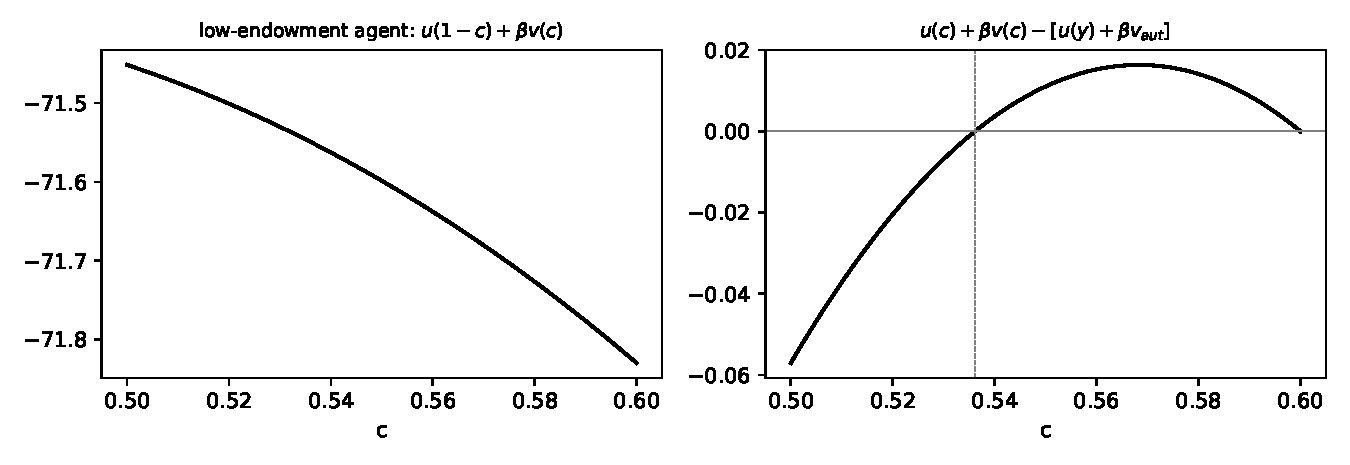
\includegraphics[width=0.85\textwidth]{figures/ch22_05.pdf}\\
{\small Figure S22.3.  The chapter's example ($\beta=.85$, $\gamma=1.1$, $y=.6$).  Left: welfare of the low-endowment agent.  Right: the high-endowment agent's participation
constraint; the optimal $c=.5361$ is where it first becomes nonnegative.}
\end{center}

\textbf{(h)}  Raising the constrained agent's continuation value instead of its current consumption would require promising it more in some future state.  But in every future
state one of the two agents has the high endowment, so one participation constraint binds, and amnesia pins the allocation at $(c,1-c)$ whatever was promised.  There is no
future state with slack in which a promise could be delivered.  Formally, the two consumption intervals are disjoint (no first-best sustainable allocation), so the ergodic set is
$\{1-c,c\}$ and every continuation value equals $v$.  Any other promise can only be delivered by moving away from the kink of $P$, which lowers total welfare, as in
Exercise 22.3(b).

\textbf{(i)}  If the same agent is rich tomorrow, both marginal rates of substitution equal $\beta$, so $q(y\given y)=.5\beta$.  If the roles switch, today's rich agent (who eats
$c$ today and $1-c$ tomorrow) has the larger ratio, $\beta u'(1-c)/u'(c)>\beta$, so $q(1-y\given y)=.5\beta\,u'(1-c)/u'(c)$.  Hence
\[
  R(y)=R(1-y)=\frac{1}{.5\beta\bigl[1+u'(1-c)/u'(c)\bigr]}\ <\ \frac1\beta ,
\]
because $c>.5$.  The rate is lower than with complete markets and no enforcement problems.  The rich agent, who is unconstrained, prices the bond; poor agents cannot borrow as
much as they would like against future high endowments, and the scarcity of claims drives their price up.  In the example, $q(y\given y)=.425$, $q(1-y\given y)=.4984$, and
$R=1.0830$, against $1/\beta=1.1765$.
\rmk{Footnote 14 of the chapter reports a risk-free rate of $1.0146$ for this example.  With $c=.536$ and the pricing formula above, the rate is $1.0830$.  A rate of $1.0146$ would
require $c=.5626$, which is not the optimal $c$.}
\end{ex}

%% ===========================================================================
%% Chapter 23. Optimal Unemployment Insurance
%% ===========================================================================
\solchapter{23}{Optimal Unemployment Insurance}

\begin{center}
\begin{minipage}{0.86\textwidth}
\small
Solutions to all 6 exercises of Chapter 23 of Ljungqvist and Sargent, \emph{Recursive Macroeconomic Theory} (4th edition, 2018).  \texttt{code/ch23.py} calibrates
Hopenhayn and Nicolini's model and solves the Bellman equation (23.2.11) for Exercise 23.1.  The other exercises are analytical.
\end{minipage}
\end{center}

\bigskip
\hrule
\bigskip

Throughout, $V$ is the promised value of an unemployed worker, $C(V)$ the insurance agency's minimum cost of delivering it, and $V^e=u(w)/(1-\beta)$ the value of
permanent employment.  Unless stated otherwise, the agency discounts at $\beta$ (it borrows and lends at $R=\beta^{-1}$).

%%---------------------------------------------------------------------------
\begin{ex}{23.1}{Optimal unemployment compensation}
The parameters are those of Section 23.2.5: one period is a week, $\beta=.999$, $u(c)=c^{1-\sigma}/(1-\sigma)$ with $\sigma=.5$ (so $u(c)=2\sqrt c$ and $u(0)=0$),
$w=100$ and $p(a)=1-e^{-ra}$.  The parameter $r$ is chosen so that the autarky hazard is $p(a^*)=.1$.  Then $V^e=u(100)/(1-\beta)=20{,}000$.

\textbf{(a)}  In autarky the worker solves (23.2.3) with first-order condition (23.2.4), $\beta re^{-ra}(V^e-V^u)=1$.  Impose $e^{-ra^*}=.9$.  The Bellman equation gives
$V_{\rm aut}(1-.9\beta)=-a^*+.1\beta V^e$, so $V^e-V_{\rm aut}=[u(w)+a^*]/(1-.9\beta)$.  Here $u(w)=(1-\beta)V^e$ and $a^*=\ln(10/9)/r$.  Combining with the first-order
condition $V^e-V_{\rm aut}=1/(.9\beta r)$ gives the closed form
\[
  r\,u(w)=\frac{1-.9\beta}{.9\beta}-\ln\frac{10}{9}\quad\Longrightarrow\quad r=3.4314\times10^{-4},
\]
with $a^*=307.05$ and $V_{\rm aut}=16{,}758.70$.  The iterative algorithm of Section 23.2.1 (guess $V^u$, get $a$ from (23.2.4), update $V^u$ from (23.2.3)) converges from
$V^u=0$ in 257 iterations to the same values, with hazard $.1000$ and expected duration 10 weeks.  Continuation values lie in $[V_{\rm aut},\,V^e-1/(\beta r)]
=[16{,}758.70,\ 17{,}082.83]$; the upper bound is the one of Section 23.2.6, which keeps search effort positive.

\textbf{(b)}  Following Section 23.2.6, we eliminate $c$ and $a$.  The binding incentive constraint gives $a(V^u)=\max\{0,\ln[r\beta(V^e-V^u)]/r\}$, and promise keeping
gives $c=u^{-1}(V+a-\beta[p(a)V^e+(1-p(a))V^u])$.  The Bellman equation (23.2.11) is then a minimization over $V^u$ alone.  We solve it by Howard policy iteration on 2001
nodes, clustered at both ends of $[V_{\rm aut},17{,}082.83]$, with $C$ interpolated linearly.  Each improvement step is a golden-section search over $V^u$.  Each
evaluation step solves exactly the linear system $C=c+\beta(1-p)\,C(V^u(\cdot))$.  Convergence takes 24 steps, and the Bellman residual is $7\times10^{-6}$.  The computed
$C$ is increasing and convex, which is the property Hopenhayn and Nicolini assume.  It satisfies the first-order relations of Section 23.2.4.  With
$p=1-e^{-ra}$, (23.2.8) and the binding (23.2.4) imply $p'/(1-p)=r$ and $\eta=C(V^u)/[r(V^e-V^u)]$, hence
\[
  C'(V)=\frac1{u'(c)}=\sqrt c=C'(V^u)+\frac{C(V^u)}{V^e-V^u}.
\]
The computed solution satisfies this to within $0.4\%$.  Since $C(V^u)>0$, it implies $C'(V^u)<C'(V)$ and $V^u<V$: benefits fall with duration.  The optimal policy
indeed has $V^u<V$ everywhere, except in a thin layer within 3 utils of $V_{\rm aut}$, where $C$ is essentially flat and the minimization is numerically ill-conditioned.

The table reports, for three initial promises: the cost $C(V_0)$; the full-information cost (Section 23.2.2: constant $c$ and $a$); and the cheapest \emph{constant}
benefit $b$ that delivers $V_0$ when the worker chooses effort freely, with its cost.  It then gives the replacement ratio $c/w$ by week of unemployment and search
effort in weeks 1 and 50.
\begin{center}
\small\setlength{\tabcolsep}{3.5pt}
\begin{tabular}{rrrrrr|ccccccc|rr}
\toprule
$V_0$ & $C(V_0)$ & full info & $b/w$ & const.\ cost & saving & wk 1 & 5 & 10 & 20 & 30 & 40 & 50 & $a_1$ & $a_{50}$\\
\midrule
16{,}850 & 210.4 & 197.2 & .161 & 215.6 & 2.4\% & .212 & .190 & .167 & .132 & .107 & .088 & .074 & 225 & 259\\
16{,}942 & 849.0 & 742.8 & .466 & 991.2 & 14.4\% & .861 & .691 & .542 & .358 & .254 & .190 & .148 & 142 & 239\\
17{,}000 & 1472.7 & 1232.1 & .628 & 2196.6 & 33.0\% & 1.496 & 1.124 & .826 & .502 & .337 & .242 & .182 & 90 & 231\\
\bottomrule
\end{tabular}
\end{center}
The middle row starts at the book's $V_0=16{,}942$.  Figure S23.1 reproduces the book's Figure 23.2.1: the replacement ratio falls from $.86$ to $.15$ over 50 weeks,
while effort rises from 142 toward the autarky level 307.  The more generous the initial promise, the steeper the decline.  Near the upper bound of $V$, delivering the
promise requires front-loading consumption above the wage.  The value of history dependence is large: relative to the best constant benefit, the optimal contract saves
$2\%$, $14\%$ and $33\%$ of the cost.  A constant benefit generous enough to deliver $V_0$ destroys search incentives (hazard $.028$ instead of $.1$ in the last case).
The full-information contract would be cheaper still.  It keeps $c$ constant (e.g.\ $c/w=.570$ for $V_0=16{,}942$) and asks for constant, higher effort ($a=230$).
\begin{center}
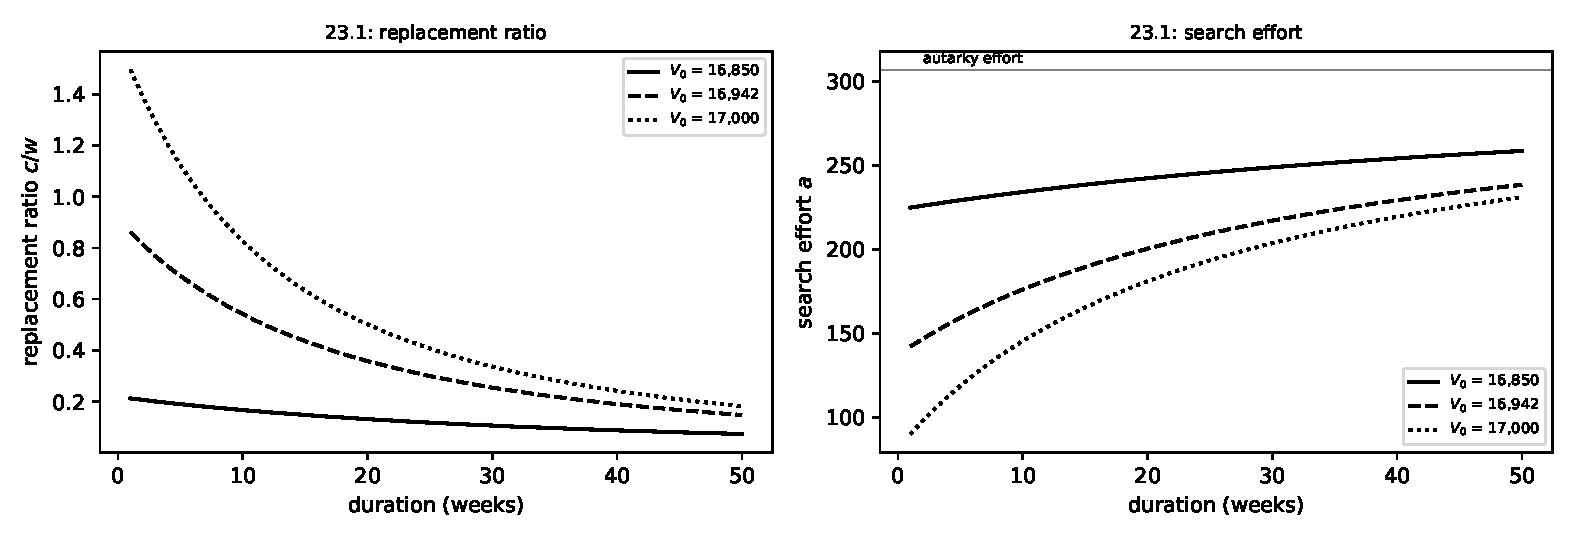
\includegraphics[width=\textwidth]{figures/ch23_01.pdf}\\
{\small Figure S23.1.  Exercise 23.1: optimal replacement ratio and search effort by duration of unemployment for three initial promised values.}
\end{center}
\end{ex}

%%---------------------------------------------------------------------------
\begin{ex}{23.2}{Taxation after employment}
Now the value of employment is a choice variable.  A worker who finds a job after the current period gets $V^e=u(w-\tau)/(1-\beta)$, and the tax $\tau$ may depend on the
history of the unemployment spell.  Since there is no incentive problem on the job, it is optimal to tax the employed worker at a constant rate.  Delivering $V^e$ to an
employed worker costs the agency
\[
  C_e(V^e)=-\frac{\tau}{1-\beta}=\frac{u^{-1}\bigl((1-\beta)V^e\bigr)-w}{1-\beta},\qquad C_e'(V^e)=\frac1{u'(w-\tau)}.
\]
The Bellman equation becomes
\[
  C(V)=\min_{c,a,V^u,V^e}\Bigl\{c+\beta\bigl[p(a)C_e(V^e)+(1-p(a))C(V^u)\bigr]\Bigr\}
\]
subject to promise keeping, $V=u(c)-a+\beta[p(a)V^e+(1-p(a))V^u]$, and the incentive constraint $\beta p'(a)(V^e-V^u)\le1$, with equality if $a>0$.  Here $V^e$ now
appears in both constraints as a control.  With multipliers $\theta$ on promise keeping and $\eta$ on the incentive constraint, the first-order conditions are
\[
  \frac1{u'(c)}=\theta,\qquad
  C'(V^u)=\theta-\eta\frac{p'(a)}{1-p(a)},\qquad
  \frac1{u'(w-\tau)}=C_e'(V^e)=\theta+\eta\frac{p'(a)}{p(a)},
\]
plus the condition for $a$.  With $C'(V)=\theta$, the incentive problem ($\eta>0$) again makes $V^u<V$, so unemployment consumption falls with duration.  It also makes
$w-\tau>c$: the reward for finding a job is delivered partly through a lower tax on the job.  As the promised $V$ falls with duration, the $V^e$ assigned to a worker who
finds a job falls as well, so the employment tax is history dependent.  In Hopenhayn and Nicolini's computations it rises with the length of the spell, which
substantially slows the decline of the replacement ratio (Section 23.2.8).  Exercise 23.5(e) proves the rising tax in a two-effort version.
\end{ex}

%%---------------------------------------------------------------------------
\begin{ex}{23.3}{Optimal unemployment compensation with unobservable wage offers}
Let $V$ be the value of an unemployed worker at the start of a period, before this period's offer is drawn.  An accepted offer $w$ is worth $u(w)/(1-\beta)$ and costs
the agency nothing.

\textbf{(a)}  With a constant benefit, $Q=\int\max\{u(w)/(1-\beta),\,u(b)+\beta Q\}\dd F(w)$.  The worker accepts iff $w\ge\bar w$, where
$u(\bar w)/(1-\beta)=u(b)+\beta Q$.  Substituting $\bar w$ into the equation for $Q$ and rearranging,
\[
  (1-\beta)\bigl[u(\bar w)-u(b)\bigr]=\beta\int_{\bar w}^{w_H}\bigl[u(w)-u(\bar w)\bigr]\frac{\dd w}{w_H-w_L} .
\]
The left side increases in $\bar w$ and the right side decreases, so $\bar w$ is unique, provided the solution lies in $[w_L,w_H]$; otherwise the worker accepts every offer.
The reservation wage rises with $b$ and is constant over the spell.

\textbf{(b)}  A contract specifies this period's reservation wage $\bar w$, the benefit $c$ if no acceptable offer arrives, and the continuation promise $V^u$.  Then
\[
  C(V)=\min_{\bar w,c,V^u}F(\bar w)\bigl[c+\beta C(V^u)\bigr]\quad\text{s.t.}\quad
  V=\int_{\bar w}^{w_H}\frac{u(w)}{1-\beta}\dd F(w)+F(\bar w)\bigl[u(c)+\beta V^u\bigr].
\]
With multiplier $\theta$, the first-order conditions are $\theta=1/u'(c)$ and $C'(V^u)=\theta$, and for $\bar w$
\[
  \frac{u(\bar w)}{1-\beta}=u(c)+\beta V^u-u'(c)\bigl[c+\beta C(V^u)\bigr].
\]
The envelope condition $C'(V)=\theta$ and convexity give $V^u=V$.  So consumption and the reservation wage are constant during the spell: full smoothing, as in
Section 23.2.2.  The reservation wage is \emph{below} the one the worker would choose given $(c,V)$, which satisfies $u(\bar w)/(1-\beta)=u(c)+\beta V$.  The agency
internalizes the cost $c+\beta C(V)$ of another period of unemployment and makes the worker accept lower offers.

\textbf{(c)}  Now the worker chooses his reservation wage.  Given $(c,V^u)$, it satisfies the incentive constraint $u(\bar w)/(1-\beta)=u(c)+\beta V^u$, and promise
keeping becomes
\[
  V=\Phi(\bar w)\equiv\frac{F(\bar w)u(\bar w)+\int_{\bar w}^{w_H}u(w)\dd F(w)}{1-\beta},\qquad \Phi'(\bar w)=\frac{F(\bar w)u'(\bar w)}{1-\beta}>0 .
\]
So the promised value pins down the reservation wage, $\bar w=\Phi^{-1}(V)$.  The agency can only choose how to deliver the utility $k=u(\bar w)/(1-\beta)$ of rejecting.
Let $G(k)=\min\{c+\beta C(V^u):u(c)+\beta V^u=k\}$.  Its first-order condition is $1/u'(c)=C'(V^u)$, and $G'(k)=1/u'(c)$.  Then $C(V)=F(\bar w)G(u(\bar w)/(1-\beta))$
with $\bar w=\Phi^{-1}(V)$, and differentiating,
\[
  C'(V)=\frac{f(\bar w)G+F(\bar w)G'\,u'(\bar w)/(1-\beta)}{\Phi'(\bar w)}=G'(k)+\frac{(1-\beta)f(\bar w)}{F(\bar w)u'(\bar w)}\,G(k)>G'(k)=C'(V^u).
\]
By convexity of $C$, $V^u<V$: promised values fall during the spell.  Along the spell $1/u'(c_t)=C'(V_{t+1})$, and $V_{t+2}<V_{t+1}$ gives
$1/u'(c_{t+1})=C'(V_{t+2})<C'(V_{t+1})=1/u'(c_t)$.  So \emph{consumption (the benefit) declines with the duration of unemployment}, and the reservation wage
$\bar w_t=\Phi^{-1}(V_t)$ declines with it.  This is Shavell and Weiss's result.  The agency cannot force acceptance, but lowering future benefits lowers the
reservation wage and shortens unemployment.  This is worth some loss of consumption smoothing.  The wedge is larger the higher the density $f(\bar w)$ of offers at the
margin relative to the probability $F(\bar w)$ of remaining unemployed.
\end{ex}

%%---------------------------------------------------------------------------
\begin{ex}{23.4}{Full unemployment insurance}
The agency chooses current consumption $c$, effort $a$, the continuation promise $V^u$ if no job is found, and the tax $\tau$ paid forever by a worker who finds a job
now.  A tax $\tau$ is worth $-\tau/(1-\beta)$ to the agency.  So
\[
  C(V)=\min_{c,a,V^u,\tau}\Bigl\{c+\beta\Bigl[-p(a)\frac{\tau}{1-\beta}+\bigl(1-p(a)\bigr)C(V^u)\Bigr]\Bigr\}
\]
subject to $V=u(c)-a+\beta[p(a)u(w-\tau)/(1-\beta)+(1-p(a))V^u]$.  Effort is observed, so there is no incentive constraint.

The name of the exercise comes from the solution.  With multiplier $\theta$ on promise keeping, the conditions for $c$ and $\tau$ are $1=\theta u'(c)$ and
$\beta p/(1-\beta)=\theta\beta p\,u'(w-\tau)/(1-\beta)$.  So $u'(w-\tau)=u'(c)$, i.e.\ $w-\tau=c$: the worker consumes the same whether employed or not.  The
condition for $V^u$ is $C'(V^u)=\theta=C'(V)$, so $V^u=V$ and $c$ stays constant during the spell.  Effort is constant too and set at its social optimum.  The first-order
condition for $a$ balances its disutility against the fall in the agency's cost when the worker leaves unemployment:
$\theta[1-\beta p'(a)(u(c)/(1-\beta)-V)]=\beta p'(a)\bigl[C(V)+c/(1-\beta)\bigr]$.  The worker is fully insured against the unemployment risk.
\end{ex}

%%---------------------------------------------------------------------------
\begin{ex}{23.5}{Two effort levels}
Write $\pi\equiv\pi(a)$ and $\Delta\pi=\pi(a)-\pi(0)>0$.

\textbf{(a)}
\[
  C(V)=\min_{c,V^u}\bigl\{c+\beta(1-\pi)C(V^u)\bigr\}\quad\text{s.t.}\quad V=u(c)-a+\beta\bigl[\pi V_e+(1-\pi)V^u\bigr]
\]
and the incentive constraint.  High effort must beat zero effort:
$u(c)-a+\beta[\pi V_e+(1-\pi)V^u]\ge u(c)+\beta[\pi(0)V_e+(1-\pi(0))V^u]$, i.e.
\[
  \beta\,\Delta\pi\,(V_e-V^u)\ge a\quad\Longleftrightarrow\quad V^u\le\hat V\equiv V_e-\frac{a}{\beta\Delta\pi}.
\]
Because effort enters utility additively and linearly, the constraint involves only the continuation value.

\textbf{(b)}  With multipliers $\theta$ and $\eta\ge0$, the first-order conditions are $1/u'(c)=\theta$ and $\beta(1-\pi)C'(V^u)=\theta\beta(1-\pi)-\eta\beta\Delta\pi$.
The envelope condition is $C'(V)=\theta$, so
\[
  C'(V^u)=C'(V)-\eta\frac{\Delta\pi}{1-\pi}.
\]
If the constraint binds ($\eta>0$), $C'(V^u)<C'(V)$ and $V^u<V$.  Next period's benefit then satisfies $1/u'(c_{t+1})=C'(V_{t+1})=C'(V^u_t)<C'(V_t)=1/u'(c_t)$, so
$c_{t+1}<c_t$: benefits decline.  With two effort levels the decline is a single step.  The constraint binds iff $V>\hat V$, and then it sets $V^u=\hat V$.  At $V=\hat V$
the unconstrained choice $V^u=V=\hat V$ satisfies the constraint with equality, so from then on the promise and the benefit $\hat c$ are constant, where
$u(\hat c)=\hat V(1-\beta(1-\pi))+a-\beta\pi V_e$.  So a worker promised $V_0>\hat V$ gets $c_0>\hat c$ in the first week of unemployment and $\hat c$ afterwards.  If
$V_0\le\hat V$ the constraint is slack and benefits are constant.

\textbf{(c)}  If $\pi(a)=\pi(0)$, the incentive constraint reads $0\ge a$, which fails: high effort cannot be induced, and it would be pointless because it does not affect
job finding.  The agency lets the worker set $a=0$.  Without an incentive constraint, $C'(V^u)=C'(V)$ gives $V^u=V$, and benefits are constant.  Benefits decline only
because declining benefits provide incentives, as the text notes after (23.2.8c).

\textbf{(d)}  With $V_e=u(w-\tau)/(1-\beta)$ chosen along with $(c,V^u)$ and cost $C_e(V_e)=[u^{-1}((1-\beta)V_e)-w]/(1-\beta)$,
\[
  C(V)=\min_{c,V^u,V_e}\bigl\{c+\beta[\pi C_e(V_e)+(1-\pi)C(V^u)]\bigr\}
\]
subject to $V=u(c)-a+\beta[\pi V_e+(1-\pi)V^u]$ and $\beta\Delta\pi(V_e-V^u)\ge a$.

\textbf{(e)}  The first-order conditions are
\[
  \frac1{u'(c)}=\theta=C'(V),\qquad C'(V^u)=\theta-\eta\frac{\Delta\pi}{1-\pi},\qquad \frac1{u'(w-\tau)}=C_e'(V_e)=\theta+\eta\frac{\Delta\pi}{\pi}.
\]
The incentive constraint always binds.  If $\eta=0$, the agency would give full insurance, $V^u=V$ and $w-\tau=c$.  Promise keeping would then imply
$V_e-V=a/(1-\beta+\beta\pi)$, and the constraint $V_e-V\ge a/(\beta\Delta\pi)$ would require $\beta\Delta\pi\ge1-\beta+\beta\pi(a)$, i.e.\ $-\beta\pi(0)\ge1-\beta$, which is
impossible.  So $\eta>0$ at every date.  Hence $V_{t+1}=V^u_t<V_t$, and the promise declines strictly and permanently over the spell.  The binding constraint fixes
$V_{e,t}=V_{t+1}+a/(\beta\Delta\pi)$, so $V_{e,t}$ declines with duration too, i.e.\ $u(w-\tau_t)$ falls.  \emph{The tax on a worker who finds a job rises with the
duration of his unemployment spell.}  Benefits also keep falling ($c_{t+1}<c_t$), and at every date $w-\tau_t>c_t$.  Unlike in subproblem A, where the decline was a
single step, the tax instrument makes both benefits and post-employment consumption decline gradually.  The agency spreads the punishment for long spells over the
worker's whole future.
\end{ex}

%%---------------------------------------------------------------------------
\begin{ex}{23.6}{Partially observed search effort}
\textbf{(a)}  A contract specifies consumption $c$, recommended effort $a$, and continuation values for an unsuccessful searcher: $V_O(\tilde a)$ if last period's effort
$\tilde a$ is observed, and $V_N$ if it is not.  Punishing an observed deviation as hard as possible is free.  So set $V_O(\tilde a)=V_{\rm aut}$ for $\tilde a\ne a$: the
lowest deliverable value, which costs $C(V_{\rm aut})=0$.  Write $V_O\equiv V_O(a)$.  The best deviation $\tilde a$ solves
$\max_{\tilde a}\{-\tilde a+\beta[p(\tilde a)V^e+(1-p(\tilde a))(dV_{\rm aut}+(1-d)V_N)]\}$, i.e.\
$\beta p'(\tilde a)[V^e-dV_{\rm aut}-(1-d)V_N]=1$ if interior.  The Bellman equation is
\[
  C(V)=\min_{c,a,V_O,V_N}\Bigl\{c+\beta\bigl(1-p(a)\bigr)\bigl[dC(V_O)+(1-d)C(V_N)\bigr]\Bigr\}
\]
subject to promise keeping, $V=u(c)-a+\beta\{p(a)V^e+(1-p(a))[dV_O+(1-d)V_N]\}$, and the global incentive constraint
\begin{multline*}
  -a+\beta\Bigl\{p(a)V^e+\bigl(1-p(a)\bigr)\bigl[dV_O+(1-d)V_N\bigr]\Bigr\}\\
  \ge\ \max_{\tilde a}\Bigl\{-\tilde a+\beta\Bigl[p(\tilde a)V^e+\bigl(1-p(\tilde a)\bigr)\bigl(dV_{\rm aut}+(1-d)V_N\bigr)\Bigr]\Bigr\},
\end{multline*}
with $V_O,V_N\ge V_{\rm aut}$.  The first-order approach of the text is inappropriate here.  Detection makes the worker's payoff jump at $\tilde a=a$, so the constraint must
be imposed against the best global deviation.

\textbf{(b)}  Let $\theta$ and $\eta\ge0$ be the multipliers and $\tilde a$ the best deviation.  By the envelope theorem, the derivative of the right side with respect to $V_N$
is $\beta(1-d)(1-p(\tilde a))$.  The first-order conditions and the envelope condition $C'(V)=\theta$ give
\[
  \frac1{u'(c)}=\theta,\qquad C'(V_O)=\theta+\eta,\qquad C'(V_N)=\theta-\eta\,\frac{p(a)-p(\tilde a)}{1-p(a)} .
\]
When the constraint binds, $p(a)>p(\tilde a)$ and so $C'(V_O)>C'(V)>C'(V_N)$, i.e.\ $V_O>V>V_N$.
\begin{itemize}
  \item After a week without a job in which effort is \emph{not} observed, the promise falls ($V_N<V$).  As in Hopenhayn and Nicolini, benefits decline with the duration of
  unmonitored unemployment.
  \item After a week in which compliant effort \emph{is} observed, the promise rises ($V_O>V$): the contract pays a bonus for verified search.  Rewarding verified compliance is
  a cheap way to provide incentives, because it pays off only in states where the planner knows the worker searched.
  \item Detected shirking sends the worker to $V_{\rm aut}$ (off the equilibrium path).
\end{itemize}
Compensation therefore depends on the whole history of verification outcomes, not just on duration.  Benefits drift down during unmonitored stretches and jump up at
each successful audit, so two workers unemployed for the same time can receive very different benefits.  The threat of detection weakens the constraint, since
$V_{\rm aut}$ replaces $V_N$ in the deviation payoff with probability $d$.  As $d\to0$ we recover Hopenhayn and Nicolini ($V_O$ irrelevant, $V_N<V$).  As $d$ grows the
constraint relaxes, and for $d$ large enough it no longer binds at the full-information contract ($\eta=0$).  Then $V_O=V_N=V$ and constant consumption, the
full-information outcome of Section 23.2.2, is implementable.
\end{ex}

%% ===========================================================================
%% Chapter 24. Credible Government Policies, I
%% ===========================================================================
\solchapter{24}{Credible Government Policies, I}

\begin{center}
\begin{minipage}{0.86\textwidth}
\small
Solutions to all 3 exercises of Chapter 24 of Ljungqvist and Sargent, \emph{Recursive Macroeconomic Theory} (4th edition, 2018).  Numbers and the figure come from
\texttt{code/ch24.py}.  For the Kydland--Prescott model of Exercise 24.3, the script iterates the APS operator to convergence, which independently checks every best and worst
value derived by hand.
\end{minipage}
\end{center}

\bigskip
\hrule
\bigskip

Notation follows the chapter.  $C$ is the set of competitive equilibria $(x,y)$ with $x=h(y)$, $r(x,y)=u(x,x,y)$ is the government's one-period payoff, and $H(x)$ is its
one-period best response.  A Nash equilibrium is a pair $(x,y)\in C$ with $y=H(x)$; the Ramsey outcome maximizes $r$ over $C$.  In the repeated economy the government
values paths by $(1-\delta)\sum_{t\ge1}\delta^{t-1}r(x_t,y_t)$.  The lemma of Section 24.6 reduces subgame perfection to one-shot incentive constraints:
\[
  (1-\delta)r(x,y)+\delta v'\ \ge\ (1-\delta)r(x,\eta)+\delta\tilde v(\eta)\quad\forall\eta,
\]
with continuation values $v'$ and $\tilde v(\eta)$ that are themselves SPE values.

%%---------------------------------------------------------------------------
\begin{ex}{24.1}{Finite repetition with multiple Nash equilibria}
\textbf{(a)}  The government's best responses are $H(x_M)=y_M$ ($10>4$) and $H(x_H)=y_M$ ($20>15$).  Of the two competitive equilibria only $(x_M,y_M)$ satisfies $y=H(x)$, so
the unique Nash equilibrium is $(x_M,y_M)$, with $v^N=10$.  The Ramsey outcome is the best competitive equilibrium, $(x_H,y_H)$, with $v^R=15$.  The government would like to
promise $y_H$, but after the public has set $x_H$ it is tempted by $y_M$, which pays 20.

\textbf{(b)}  No.  In the last period any SPE must play a one-period Nash equilibrium after every history.  Since $(x_M,y_M)$ is the only one, the second-period
outcome, and hence the continuation value, is the same whatever the government does in period 1.  Then in period 1 the government simply maximizes its current payoff.
Given $x_H$, it chooses $y_M$ and gains $20-15=5$ at no future cost.  ``Reverting to Nash'' is no punishment when Nash is also what happens after conformity.

\textbf{(c)}  No, in neither period.  By backward induction the third period plays $(x_M,y_M)$ after every history.  The second period then has a history-independent
continuation, so it must also play the stage Nash equilibrium, and the same argument applies to the first period.  With a unique one-period Nash equilibrium, the finitely
repeated economy has a unique SPE: Nash in every period.

\textbf{(d)}  Now $H(x_L)=y_L$ ($3>1>0$), $H(x_M)=y_M$ ($10>7>4$) and $H(x_H)=y_M$ ($20>15>9$).  The competitive equilibria $(x_L,y_L)$ and $(x_M,y_M)$ satisfy $y=H(x)$, but
$(x_H,y_H)$ does not.  So there are two Nash equilibria, a bad one $(x_L,y_L)$ with value 3 and a good one $(x_M,y_M)$ with value 10.  Ramsey is still $(x_H,y_H)$, with value 15.

\textbf{(e)}  The multiplicity of Nash equilibria provides the punishment (Benoit and Krishna's idea).  Strategy profile: in period 1 play $(x_H,y_H)$.  In period 2 play the
good Nash equilibrium $(x_M,y_M)$ if the period-1 outcome was $(x_H,y_H)$, and the bad one $(x_L,y_L)$ otherwise.  Period-2 play is a one-period Nash equilibrium after
every history, so it is subgame perfect.  In period 1, $x_H=h(y_H)$ is a competitive equilibrium.  The government's best deviation is $y_M$, and it does not deviate if
\[
  15+10\delta\ \ge\ 20+3\delta\iff\delta\ge\tfrac57\approx.714 .
\]
(Multiplying both sides by $1-\delta$ gives the normalized criterion and changes nothing.)  So the profile is an SPE exactly when $\delta\ge5/7$.

\textbf{(f)}  With $\delta=.8\ (>5/7)$, consider the following profile.
\begin{itemize}
  \item Period 1: $(x_H,y_H)$.
  \item Period 2: $(x_H,y_H)$ if the period-1 outcome was $(x_H,y_H)$; otherwise $(x_L,y_L)$.
  \item Period 3: $(x_M,y_M)$ if the outcomes of periods 1 and 2 were both $(x_H,y_H)$; otherwise $(x_L,y_L)$.
\end{itemize}
Period-3 play is a stage Nash equilibrium after every history.  In period 2 on the path, conforming gives $15+.8\cdot10=23$ and deviating gives $20+.8\cdot3=22.4$.  Off the
path, period 2 plays a stage Nash equilibrium followed by a history-independent continuation.  In period 1, conforming gives $15+.8\cdot15+.64\cdot10=33.4$ and deviating
gives $20+.8\cdot3+.64\cdot3=24.32$.  So Ramsey is supported in the first two periods.  (The period-1 constraint alone would hold for $\delta\ge.347$; the binding
constraint is the period-2 one, $\delta\ge5/7$.)

The SPE is \emph{not unique}, although its outcome path is.  On the path, period 3 must play $(x_M,y_M)$, because otherwise the period-2 constraint $15+.8w_3^{\rm on}\ge20+.8w_3^{\rm off}$
fails.  After a period-2 deviation, period 3 must play $(x_L,y_L)$, because $23\ge20+.8w$ requires $w\le3.75$.  But the punishment after a \emph{period-1} deviation can be
chosen in several ways.  Its continuation can be $(x_L,y_L)$ then $(x_M,y_M)$ (the deviator gets $20+2.4+6.4=28.8$), or $(x_M,y_M)$ then $(x_L,y_L)$ ($20+8+1.92=29.92$).
Both deter the deviation ($<33.4$) and give different SPEs with the same outcome path.  Punishments $(x_M,y_M)$ twice ($34.4$) or the good continuation ($38.4$) would not deter it.
\end{ex}

%%---------------------------------------------------------------------------
\begin{ex}{24.2}{An economy without a one-period Nash equilibrium (Stokey 1989)}
\textbf{(a)}  In a Ramsey plan the government moves first and is bound by its choice.  It picks $y\in Y$ knowing that the public responds with the competitive equilibrium
$x=h(y)$.  So it solves $\max_{(x,y)\in C}r(x,y)$ (Definitions 3--4).  Here $h(y_L)=x_L$ and $h(y_H)=x_H$, and $\max\{0,10\}=10$, so the Ramsey outcome is $(x_H,y_H)$, with $v^R=10$.

\textbf{(b)}  A pure-strategy Nash equilibrium is a pair $(x^N,y^N)$ such that $(x^N,y^N)\in C$ (the public has no incentive to deviate given $y^N$) and
$r(x^N,y^N)=\max_\eta r(x^N,\eta)$ (the government has no incentive to deviate given $x^N$), i.e.\ $y^N=H(x^N)$.

\textbf{(c)}  $H(x_L)=y_H$ (since $1>0$) and $H(x_H)=y_L$ (since $20>10$).  The competitive equilibrium $(x_L,y_L)$ has $H(x_L)=y_H\ne y_L$, and $(x_H,y_H)$ has $H(x_H)=y_L\ne y_H$.
So no competitive equilibrium is a best response to itself, and there is no pure-strategy Nash equilibrium.  Low inflation expectations tempt the government to inflate, and
high expectations tempt it to disinflate.

\textbf{(d)}  A strategy profile $\sigma=(\sigma^h,\sigma^g)$ maps each history $(x^{t-1},y^{t-1})$ into actions $(x_t,y_t)$.  It is an SPE if for every $t$ and every history
(i) $(x_t,y_t)=\sigma_t(x^{t-1},y^{t-1})\in C$, and (ii) for every $\eta\in Y$,
$(1-\delta)r(x_t,y_t)+\delta V_g(\sigma|_{(x^t,y^t)})\ge(1-\delta)r(x_t,\eta)+\delta V_g(\sigma|_{(x^t;y^{t-1},\eta)})$ (Definition 6).

\textbf{(e)}  \emph{Lower bound.}  Let $\underline v$ be the lowest SPE value, and consider the SPE that attains it, with first-period outcome $(x,y)\in C$.  The government can
always play its one-period best response, and the worst it can then face is $\underline v$, so
$\underline v\ge(1-\delta)\max_\eta r(x,\eta)+\delta\underline v$, i.e.\ $\underline v\ge\max_\eta r(x,\eta)\ge\min_{y}\max_\eta r(h(y),\eta)$.  Here
$\min\{\max_\eta r(x_L,\eta),\max_\eta r(x_H,\eta)\}=\min\{1,20\}=1$.  \emph{Attainment.}  The bound is reached by starting with the ``stick'' $(x_L,y_L)$ (payoff 0,
temptation 1), with deviations restarting the equilibrium.  The binding constraint $\underline v=(1-\delta)\cdot0+\delta v_1=(1-\delta)\cdot1+\delta\underline v$ gives $\underline v=1$
and $v_1=1/\delta$, which must itself be an SPE value.  At the discount factor of part (f) it is (parts (h)--(k)), so the worst SPE value is $\underline v=1$.  Part (l)
discusses discount factors for which the needed continuation values are not available.

\textbf{(f)}  Yes.  With the worst SPE as punishment, the incentive constraint for Ramsey is
\[
  v^R=10\ \ge\ (1-\delta)\,r(x_H,y_L)+\delta\underline v=(1-.8913)\cdot20+.8913\cdot1=3.066 .
\]
A recursive SPE (Definition 12) has states $v_j=\delta^{-j}$, $j=0,1,\dots,20$.  Note $v_0=1$ and $v_{20}=\delta^{-20}=10$ because $\delta^{20}=1/10$.  Its prescriptions are
\begin{align*}
  (z^h,z^g)(v_j)&=(x_L,y_L)\ \ (j<20),\qquad (z^h,z^g)(v_{20})=(x_H,y_H),\\
  \mathcal V(v_j,x,y)&=\begin{cases}v_{\min\{j+1,20\}}&\text{if }(x,y)=(z^h,z^g)(v_j),\\ v_0&\text{otherwise,}\end{cases}
\end{align*}
starting from $v_{20}=10$.  Promise keeping holds: $(1-\delta)\cdot0+\delta v_{j+1}=\delta^{-j}=v_j$ for $j<20$, and $(1-\delta)10+\delta\cdot10=10$.  The incentive constraints hold:
at $v_j$, $j<20$, $v_j\ge(1-\delta)\cdot1+\delta\cdot1=1$; at $v_{20}$, $10\ge3.066$.  On the path, Ramsey is played forever.  Any deviation starts the worst SPE.

\textbf{(g)}  The best SPE value cannot exceed $\max_Cr=10$, and (f) attains it: $\bar v=v^R=10$.

\textbf{(h)}  The worst SPE constructed in (f) (state $v_0$) has the path
\[
  (x_L,y_L)\ \text{for } t=1,\dots,20,\qquad (x_H,y_H)\ \text{for } t\ge21,
\]
with value $\delta^{20}\cdot10=1$.  Each period of the stick raises the promised value by the factor $1/\delta$ until it reaches the Ramsey value.  The discount factor
$(1/10)^{1/20}$ is chosen so that this happens after exactly 20 periods.  This is the path generated by the recursion of parts (i)--(k).

\textbf{(i)}  Adherence to the worst SPE requires $1=(1-\delta)\cdot0+\delta v_1$, so $v_1=\delta^{-1}=1.12202$.  $\sigma_1$ starts with the stick again: its path is 19 periods
of $(x_L,y_L)$ followed by $(x_H,y_H)$ forever.

\textbf{(j)}  Adherence to the first-period outcome $(x_L,y_L)$ of $\sigma_1$ requires $v_1=\delta v_2$, so $v_2=\delta^{-2}=1.25893$.  The path of $\sigma_2$ is 18 periods of
$(x_L,y_L)$, then Ramsey forever.

\textbf{(k)}  In general $v_j=\delta^{-j}=10^{j/20}$ and $\sigma_j$ plays $(x_L,y_L)$ for $20-j$ periods and then $(x_H,y_H)$ forever, for $j=1,\dots,20$.  At $j=20$, $v_{20}=10=v^R$
and $\sigma_{20}$ is Ramsey forever; for $j\ge20$, $v_j=10$.  The values are
$1.122,\ 1.259,\ 1.413,\ 1.585,\ 1.778,\ 1.995,\ 2.239,\ 2.512,\ 2.818,\ 3.162,\ \dots,\ 7.943,\ 8.913,\ 10$.  Every $\sigma_j$ satisfies its incentive constraints, since $v_j\ge1$
in stick periods and $10\ge3.066$ in Ramsey periods.

\textbf{(l)}  Ramsey repetition is an SPE if and only if some SPE value $w$ satisfies $10\ge(1-\delta)20+\delta w$, i.e.\ $w\le20-10/\delta$.  Since every SPE value is at least 1,
this requires $20-10/\delta\ge1$, i.e.
\[
  \delta\ \ge\ \tfrac{10}{19}=.5263 .
\]
If the value set is an interval, as the chapter's APS construction presumes (e.g.\ with a public randomization device), the worst value $1$ is available.  Then
$\delta=10/19$ is the answer: at $\delta=10/19$ the stick $(x_L,y_L)$ with continuation value $1/\delta=1.9\in[1,10]$ delivers 1.

\rmk{With pure strategies and no randomization this bound is not attained, because SPE values are restricted to values of $\{L,H\}$ paths.  For $\delta<.6466$ a period
of $(x_H,y_H)$ can never be followed by $(x_L,y_L)$: the constraint $(1-\delta)10+\delta v'\ge(1-\delta)20+\delta\cdot1$ fails for every $v'\le10\delta$.  So every SPE path has the
form $L^kH^\infty$, with value $10\delta^k$.  Path $L^k H^\infty$ is an SPE (with itself as punishment) if and only if $10\delta^k\ge1$ and $10\ge20(1-\delta)+\delta\cdot10\delta^k$.  So
Ramsey is sustainable if and only if some integer $k$ has $.1\le\delta^k\le2-1/\delta$.  The smallest such $\delta$ is the root of $\delta+\delta^2+\delta^3=1$, namely
$\delta^*=.543689$ (with $k=3$), and every larger $\delta$ also works (\texttt{ch24.py} checks this on a fine grid).  At $\delta^*$ the worst SPE is three periods of
$(x_L,y_L)$ followed by Ramsey, with value $10\delta^{*3}=1.607=20-10/\delta^*$.  For $\delta<\delta^*$ there is no pure-strategy SPE at all, because $L^\infty$ is worth $0<1$.}
\end{ex}

%%---------------------------------------------------------------------------
\begin{ex}{24.3}{Worst and best SPEs in the Kydland--Prescott model}
\textbf{(a)}  Given $y$, a forecaster maximizes $-.5(y-\xi)^2$ by setting $\xi=y$.  All forecasters do the same, so $x=\xi=y$, and then $U=U^*-\theta(y-y)=U^*$.  Hence
$C=\{(x,y):x=y\in[0,10]\}$, $h(y)=y$, and $r(h(y),y)=-.5(U^{*2}+y^2)$.

\textbf{(b)}  Given expectations $x$, the best response is $H(x)=\arg\max_{y\in[0,10]}r(x,y)$.  The first-order condition $\theta(U^*-\theta(y-x))=y$ gives
\[
  H(x)=\min\Bigl\{10,\ \frac{\theta U^*+\theta^2x}{1+\theta^2}\Bigr\},
\]
which is always positive; with $U^*=5$, $\theta=1$, $H(x)=(5+x)/2\in[2.5,7.5]$.  Given expectations, surprise inflation lowers unemployment.

\textbf{(c)}  A Nash equilibrium is $(x,y)\in C$ with $y=H(x)$.  Setting $x=y$ in $y(1+\theta^2)=\theta U^*+\theta^2y$ gives $y^N=x^N=\theta U^*$ (assuming $\theta U^*\le10$), with $U=U^*$ and
$v^N=-.5(1+\theta^2)U^{*2}$.  For $U^*=5$, $\theta=1$: $y^N=5$ and $v^N=-25$.

\textbf{(d)}  The Ramsey problem is $\max_{y}r(h(y),y)=\max_y-.5(U^{*2}+y^2)$, so $y^R=x^R=0$ and $v^R=-.5U^{*2}$ ($-12.5$ for $U^*=5$).  Committing to zero inflation removes the
inflation bias and costs no unemployment, because unemployment equals $U^*$ in every competitive equilibrium.

\textbf{(e)}  $v^R-v^N=.5\theta^2U^{*2}>0$.  The Nash inflation bias $\theta U^*$ buys no unemployment reduction.

\textbf{(f)}  As in Definition 6: a profile $\sigma=(\sigma^h,\sigma^g)$ of history-dependent rules such that after every history (i) $x_t=y_t$ (forecasts equal the government's
prescribed action, a competitive equilibrium) and (ii) for every $\eta\in[0,10]$,
$(1-\delta)r(x_t,y_t)+\delta V_g(\sigma|_{(x^t,y^t)})\ge(1-\delta)r(x_t,\eta)+\delta V_g(\sigma|_{(x^t;y^{t-1},\eta)})$.

\textbf{(g)}  As in Definition 12: a recursive strategy $(v_1,z^h,z^g,\mathcal V)$ with $x_t=z^h(v_t)$, $y_t=z^g(v_t)$, $v_{t+1}=\mathcal V(v_t,x_t,y_t)$ and $v_1\in V$ is an SPE if, for every
promised value $v$ it can reach, (1) $z^h(v)=z^g(v)$; (2) $\mathcal V(v,z^h(v),\eta)\in V$ for all $\eta$; and (3)
$v=(1-\delta)r(z^h(v),z^g(v))+\delta\mathcal V(v,z^h(v),z^g(v))\ge(1-\delta)r(z^h(v),\eta)+\delta\mathcal V(v,z^h(v),\eta)$ for all $\eta$.

\textbf{(h)}  Take $v_1=v^N$, $z^h(v)=z^g(v)=\theta U^*$ and $\mathcal V\equiv v^N$.  Condition (1) holds, and (2) holds because $v^N$ is the value of this very strategy.  Condition (3)
reduces to $r(y^N,y^N)\ge r(y^N,\eta)$ for all $\eta$, which holds because $y^N=H(x^N)$.

\textbf{(i)}  With $U^*=5$, $\theta=1$, the deviation payoff from a competitive equilibrium $(y,y)$ is
\[
  r(y,H(y))=\max_\eta r(y,\eta)=-\Bigl(\frac{5+y}{2}\Bigr)^2 .
\]
To see this, note that $H(y)=(5+y)/2$ and $U=5-(H(y)-y)=(5+y)/2$, so $r=-.5(U^2+H^2)=-H^2$.  The method has two steps.
\begin{enumerate}
  \item \emph{Lower bound.}  Let $\underline v$ be the worst SPE value and $(y,y)$ the first-period outcome of an SPE that attains it.  Deviating to $H(y)$ yields at least
  $(1-\delta)r(y,H(y))+\delta\underline v$, so $\underline v\ge r(y,H(y))\ge\min_{y\in[0,10]}r(y,H(y))=-56.25$, attained at $y=10$.
  \item \emph{Attainment.}  Candidate: the stick $y^\#=10$ (so $x=10$, $r(10,10)=-62.5$), with any deviation restarting the equilibrium.  The binding incentive constraint
  $\underline v=(1-\delta)r(10,10)+\delta v_1=(1-\delta)r(10,H(10))+\delta\underline v$ gives $\underline v=-56.25$ and
  \[
    v_1=\frac{\underline v-(1-\delta)r(10,10)}{\delta}=\frac{-56.25+3.125}{.95}=-55.921 .
  \]
  It remains to check that $v_1$ is an SPE value.  The best SPE value, with $\underline v$ as punishment, is Ramsey, because
  $r(0,0)=-12.5\ge(1-\delta)r(0,H(0))+\delta\underline v=.05(-6.25)+.95(-56.25)=-53.75$.  So $v_1\in[\underline v,\bar v]=[-56.25,-12.5]$, and part (j) constructs an SPE
  that delivers it.
\end{enumerate}
Hence the worst SPE value is $-56.25$.  As an independent check, \texttt{ch24.py} iterates the APS operator on intervals, starting from $[\min_Cr,\max_Cr]=[-62.5,-12.5]$.  It
converges to $[-56.25,-12.5]$.

The other values are:
\begin{itemize}
  \item repeated Ramsey, $v^R=-12.5$ (an SPE here);
  \item repeated Nash, $v^N=-25$;
  \item Abreu's stick-and-carrot, with one period of the stick $y=10$ followed by Ramsey forever: $\tilde v=.05(-62.5)+.95(-12.5)=-15$.
\end{itemize}
Abreu's profile is an SPE, since $\tilde v\ge r(10,H(10))=-56.25$ is its binding self-enforcing constraint.  But with $\delta=.95$ one period of stick is too mild: $\tilde v=-15$ is
\emph{better} for the government than Nash.  The worst value $-56.25$ needs a much longer or harsher stick.

\textbf{(j)}  A recursive SPE with two states attains the worst value (the chapter's method 3).
\begin{itemize}
  \item State $\underline v=-56.25$: play $x=y=10$.  If this is observed, move to $v_1$; after any deviation, stay at $\underline v$.
  \item State $v_1=-55.921$: play $x=y=\tilde y$, where $r(\tilde y,\tilde y)=v_1$, i.e.\ $\tilde y=\sqrt{-2v_1-25}=9.3189$.  If this is observed, stay at $v_1$; after any deviation,
  move to $\underline v$.
\end{itemize}
Start at $\underline v$.  Promise keeping: $.05(-62.5)+.95v_1=-56.25$, and $v_1=r(\tilde y,\tilde y)$ is stationary.  Incentives: at $\underline v$ the constraint holds with equality
($\underline v=r(10,H(10))$).  At $v_1$, $-55.921\ge.05\,r(\tilde y,H(\tilde y))+.95(-56.25)=.05(-51.26)-53.44=-56.000$.  The outcome path is $y_1=10$, then $y_t=9.3189$ forever.
Method 1 also works: $y=10$ for 40 periods, with the promised value rising from $-56.25$ to $-13.867$, then $y=7.393$ once, then Ramsey forever.  (At the transition,
$-13.867\ge-55.357$.)  So the worst value can be attained with a path that ends in Ramsey.

\textbf{(k)}  Ramsey with Nash reversion requires $v^R\ge(1-\delta)r(0,H(0))+\delta v^N$, i.e.\ $-12.5\ge-6.25(1-\delta)-25\delta$, i.e.\ $18.75\,\delta\ge6.25$.  So $\delta_c=1/3$.

\textbf{(l)}  With the worst SPE as punishment, the condition is $-12.5\ge-6.25(1-\delta)-56.25\delta$, i.e.\ $50\delta\ge6.25$, so $\tilde\delta_c=1/8$.  This uses the worst value
$-56.25$, which is available at $\tilde\delta_c$.  There the continuation value needed after the stick is $v_1=(-56.25+.875\cdot62.5)/.125=-12.5=v^R$, so Abreu's stick-and-carrot
(one period at $y=10$, then Ramsey) is exactly the worst SPE, and the worst value at $\tilde\delta_c$ is $-56.25$.  For $\delta<1/8$ the needed $v_1$ would exceed the best value,
the worst value rises above $-56.25$, and Ramsey is not sustainable at all (Figure S24.1).

\textbf{(m)}  For $\delta=.08<\tilde\delta_c$, neither $y=10$ as a stick nor Ramsey as a carrot is available.  The best and worst SPEs support each other.  The worst is a stick
$y_{lo}$ followed by the best SPE; the best is a stationary $y_{hi}$ whose deviations are punished by the worst.  Both incentive constraints bind, which gives the system (24.13.5)--(24.13.8):
\[
  \underline v=r(y_{lo},H(y_{lo})),\quad \bar v=\frac{1-\delta}{\delta}\bigl[\underline v-r(y_{lo},y_{lo})\bigr]+\underline v,\quad
  \bar v=r(y_{hi},y_{hi}),\quad \bar v=(1-\delta)r(y_{hi},H(y_{hi}))+\delta\underline v .
\]
With $r(y,y)=-.5(25+y^2)$ and $r(y,H(y))=-((5+y)/2)^2$, the solution is
\[
  y_{lo}=8.2,\qquad y_{hi}=1.8,\qquad \underline v=-6.6^2=-43.56,\qquad \bar v=-.5(25+1.8^2)=-14.12 .
\]
Check: $.92(-.5(25+8.2^2))+.08(-14.12)=-43.56$ and $.92(-3.4^2)+.08(-43.56)=-14.12$.  The APS iteration gives the same interval $[-43.56,-14.12]$.  Figure S24.1 shows how both values
depend on $\delta$.  Below $1/8$ the set of SPE values shrinks toward the Nash value $-25$ as $\delta\to0$.
\begin{center}
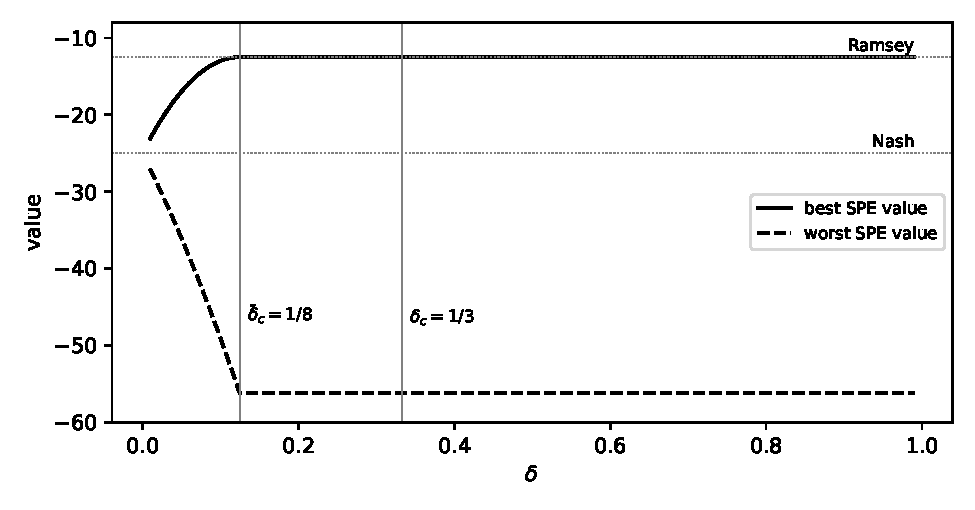
\includegraphics[width=0.8\textwidth]{figures/ch24_03.pdf}\\
{\small Figure S24.1.  Best and worst SPE values in the Kydland--Prescott example ($U^*=5$, $\theta=1$), from APS iteration.  For $\delta\ge1/8$ they are the Ramsey value $-12.5$ and
$\min_yr(y,H(y))=-56.25$.}
\end{center}
\end{ex}

%% ===========================================================================
%% Chapter 26. Two Topics in International Trade
%% ===========================================================================
\solchapter{26}{Two Topics in International Trade}

\begin{center}
\begin{minipage}{0.86\textwidth}
\small
Solutions to both exercises of Chapter 26 of Ljungqvist and Sargent, \emph{Recursive Macroeconomic Theory} (4th edition, 2018).  Both concern the Bond--Park model of
gradualism in trade policy (Section 26.3).  Numbers and the figure come from \texttt{code/ch26.py}, which also checks the closed-form constrained Pareto frontier by value-function
iteration on the Bellman equation (26.3.26).
\end{minipage}
\end{center}

\bigskip
\hrule
\bigskip

Recall the setting.  Country $L$ sets a tariff $t_L\ge0$ and country $S$ makes a voluntary transfer $e_S\ge0$, simultaneously, every period.  Payoffs are $r_L=u_L(t_L)+e_S$ and
$r_S=u_S(t_L)-e_S$, and deviations are punished by reversion to the static Nash equilibrium $(t_L^N,0)$, with values $v_i^N=u_i(t_L^N)/(1-\beta)$.  Write $W=u_W(0)/(1-\beta)$ for
the value of free trade to the world.  The constrained Pareto frontier $P(v_L)$ solves (26.3.26)--(26.3.27): maximize $u_S(t_L)-e_S+\beta P(y)$ subject to promise keeping
$u_L(t_L)+e_S+\beta y\ge v_L$ (multiplier $\theta$), $L$'s participation constraint $u_L(t_L)+\beta y\ge u_L(t_L^N)+\beta v_L^N=v_L^N$ (multiplier $\mu_L$; the transfer $e_S$ cancels
because a deviating $L$ keeps it), and $S$'s participation constraint $-e_S+\beta P(y)\ge\beta v_S^N$ (multiplier $\mu_S$).

%%---------------------------------------------------------------------------
\begin{ex}{26.1}{A quadratic Bond--Park economy}
\emph{Preliminaries.}  The small country's payoff is $u_S=u_W-u_L=\frac18-\frac12t_L$, which is linear and decreasing.  The functions have the properties used in Section 26.3: $u_L$ is
strictly concave with $u_L'(0)=\frac12>0$, and $u_W$ is strictly concave with $u_W'(0)=0$ and $u_W'(t)<0$ for $t>0$.  The parameter $\gamma_S$ enters only through the
upper bound $t_L\le1-\gamma_S=.6$ on tariffs consistent with trade.  That bound does not bind, so the Nash tariff is $t_L^N=\min\{\arg\max u_L,\,1-\gamma_S\}=\min\{.5,.6\}=.5$.
Then
\[
  u_L(t_L^N)=0,\quad u_L(0)=-\tfrac18,\quad u_S(0)=\tfrac18,\quad u_S(t_L^N)=-\tfrac18,\quad u_W(0)=0,
\]
so $v_L^N=0$, $v_S^N=-\frac1{8(1-\beta)}$ and $W=0$.  The unconstrained frontier is $v_S=W-v_L=-v_L$.

\textbf{(a)}  By (26.3.23),
\[
  \beta_c=\sqrt{\frac{u_L(t_L^N)-u_L(0)}{u_S(0)-u_S(t_L^N)}}=\sqrt{\frac{1/8}{1/4}}=\frac1{\sqrt2}=.70711 .
\]
For $\beta\in(\beta_c,1)$, (26.3.21)--(26.3.22) give
\[
  v_L^*=\frac{v_L^N-u_L(0)}{\beta}=\frac1{8\beta},\qquad
  v_L^{**}=\frac{u_L(0)+\beta\bigl(u_S(0)-u_S(t_L^N)\bigr)}{1-\beta}=\frac{2\beta-1}{8(1-\beta)} .
\]
Indeed $v_L^*<v_L^{**}$ if and only if $1-\beta<\beta(2\beta-1)$, i.e.\ $2\beta^2>1$, i.e.\ $\beta>\beta_c$.  The corresponding time-invariant transfers (26.3.18) and (26.3.20) are
$e_{S\min}=1/(8\beta)$ and $e_{S\max}=\beta/4$.  The largest value $L$ can be promised (reached in part (b)) is $v_L^{\max}=u_L(t_L^N)+\beta(W-v_S^N)=\beta/(8(1-\beta))$.
\begin{center}
\small
\begin{tabular}{ccccccc}
\toprule
$\beta$ & $v_L^*$ & $v_L^{**}$ & $v_L^{\max}$ & $v_S^N$ & $e_{S\min}$ & $e_{S\max}$\\
\midrule
.75 & .16667 & .25000 & .37500 & $-.50000$ & .16667 & .18750\\
.80 & .15625 & .37500 & .50000 & $-.62500$ & .15625 & .20000\\
.90 & .13889 & 1.00000 & 1.12500 & $-1.25000$ & .13889 & .22500\\
.95 & .13158 & 2.25000 & 2.37500 & $-2.50000$ & .13158 & .23750\\
\bottomrule
\end{tabular}
\end{center}

\textbf{(b)}  The frontier is defined on $[v_L^N,v_L^{\max}]$ and has two pieces.
\begin{itemize}
  \item \emph{Regions III and I}, $v_L^N\le v_L\le v_L^{**}$: $P(v_L)=W-v_L=-v_L$.  In both regions tariffs are zero from the start (Section 26.3.9), and transfers alone
  deliver $v_L$ (constant in region I, rising once in region III), so the frontier coincides with the unconstrained one.
  \item \emph{Region II}, $v_L^{**}<v_L\le v_L^{\max}$: here $S$'s participation constraint binds.  Solve (26.3.35) for a given $\theta>1$.  First, (26.3.35a),
  $-\frac12+\theta(\frac12-t_L)=0$, gives
  \[
    t_L=\tfrac12\bigl(1-\theta^{-1}\bigr)\in(0,t_L^N).
  \]
  Next, (26.3.35c) and (26.3.35e) give $e_S+\beta y=\beta(W-v_S^N)=\beta/(8(1-\beta))$; only this sum is determined.  Then (26.3.35b) gives
  $v_L=u_L(t_L)+\beta(W-v_S^N)=v_L^{\max}-\frac12(\frac12-t_L)^2$, and (26.3.35d), with (26.3.35c), gives $P(v_L)=u_S(t_L)+\beta v_S^N$.  Eliminating $t_L$,
  \[
    t_L=\tfrac12-\sqrt{2(v_L^{\max}-v_L)},\qquad \theta=\frac{1}{2\sqrt{2(v_L^{\max}-v_L)}},\qquad P(v_L)=v_S^N+\sqrt{\tfrac12\bigl(v_L^{\max}-v_L\bigr)} .
  \]
\end{itemize}
So in region II the frontier is an arc of the parabola $(v_S-v_S^N)^2=\frac12(v_L^{\max}-v_L)$.  At $v_L^{**}$ we have $v_L^{\max}-v_L^{**}=\frac18$, so $P=v_S^N+\frac14=W-v_L^{**}$ and
$P'=-1$ (smooth pasting, $\theta=1$, $t_L=0$).  At $v_L^{\max}$, $t_L=t_L^N$, $P=v_S^N$ and the slope $-\theta$ is $-\infty$.  Throughout region II, $P'(v_L)=-\theta$, as
the envelope condition requires.  The frontier is concave and lies strictly inside the unconstrained frontier on $(v_L^{**},v_L^{\max}]$ because the period-0 tariff is distorting.
For $\beta=.8$:
\begin{center}
\small
\begin{tabular}{cccccc}
\toprule
$v_L$ & .375 & .400 & .425 & .450 & .475\\
\midrule
$t_L$ (period 0) & 0 & .0528 & .1127 & .1838 & .2764\\
$\theta$ & 1 & 1.118 & 1.291 & 1.581 & 2.236\\
$P(v_L)$ & $-.3750$ & $-.4014$ & $-.4314$ & $-.4669$ & $-.5132$\\
\bottomrule
\end{tabular}
\end{center}
From $t=1$ on the economy is in region I with $t_L'=0$ and a constant transfer $e_S'=(1-\beta)y-u_L(0)$.  Any $y\in[v_L^*,v_L^{**}]$ can be used, with
$e_S=\beta/(8(1-\beta))-\beta y$.  For $\beta=.8$ ($e_S+\beta y=.5$): $y=v_L^{**}$ gives constant transfers $e_S=e_S'=.2=e_{S\max}$, while $y=v_L^*$ gives $e_S=.375$ and
$e_S'=.15625=e_{S\min}$.  In every case $e_S'\le e_S$, as the chapter shows, and \texttt{ch26.py} checks promise keeping and both participation constraints.

\emph{Numerical check.}  \texttt{ch26.py} iterates on the Bellman operator (26.3.26)--(26.3.27) for $\beta=.8$ on a grid of 401 promised values in $[v_L^N,W-v_S^N]$ and 601 tariffs in
$[0,1-\gamma_S]$.  It starts from the unconstrained frontier, an upper bound on $P$, and uses the smallest transfer that keeps the promise.  The iteration converges after two
steps (the optimal continuation values lie in region I, where the starting guess is already correct).  It shrinks the domain to $[0,.5]=[v_L^N,v_L^{\max}]$, matches the
closed form exactly on regions III and I, and matches it to $4\times10^{-4}$ in region II, where the tariff grid (step $.001$) limits accuracy.  Figure S26.1 plots the frontiers.
\begin{center}
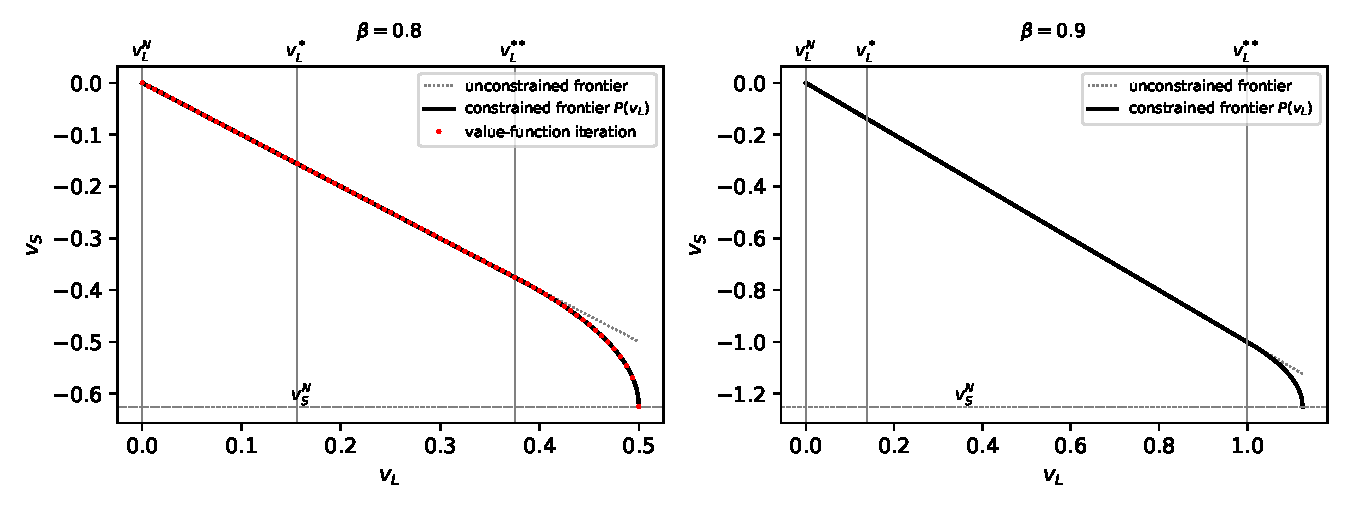
\includegraphics[width=0.95\textwidth]{figures/ch26_01.pdf}\\
{\small Figure S26.1.  Constrained Pareto frontier $v_S=P(v_L)$ for $\beta=.8$ and $\beta=.9$.  It is linear, on the unconstrained frontier, up to $v_L^{**}$, and then bends down to
$(v_L^{\max},v_S^N)$.  The dots for $\beta=.8$ are the value-function iteration.}
\end{center}

\textbf{(c)}  In region III, $v_L\in(v_L^N,v_L^*)=(0,\frac1{8\beta})$.  Follow (26.3.36) with $t_L=0$ from the start.  $L$'s participation constraint holds with equality but
with $\mu_L=0$, so (26.3.36c) gives the continuation value; (26.3.36b) gives the period-0 transfer; and the stationary region-I rule gives the transfer from period 1 on:
\[
  y=\frac{v_L^N-u_L(0)}{\beta}=v_L^*=\frac1{8\beta},\qquad
  e_S=v_L-u_L(0)-\beta y=v_L-v_L^N=v_L,
\]
\[
  e_S'=(1-\beta)y-u_L(0)=\frac1{8\beta}.
\]
Also $P(v_L)=-v_L$ and $P(y)=-\frac1{8\beta}$.  Transfers \emph{rise} from $e_S=v_L$ to $e_S'=v_L^*=e_{S\min}$ and then stay constant; $e_S'-e_S=y-v_L>0$.  $S$'s participation
constraints hold: at $t=0$, $-e_S+\beta P(y)=-v_L-\frac18\ge\beta v_S^N=-\frac{\beta}{8(1-\beta)}$ because $v_L<v_L^*<v_L^{**}$, and from $t=1$ on, $-e_S'+\beta P(y)=-\frac{1+\beta}{8\beta}\ge\beta v_S^N$
because $1-\beta^2\le\beta^2$, i.e.\ $\beta\ge\beta_c$.  For $\beta=.8$ ($v_L^*=.15625$):
\begin{center}
\small
\begin{tabular}{ccccc}
\toprule
$v_L$ & $y$ & $e_S$ & $e_S'$ & admissible $y$\\
\midrule
0 & .15625 & 0 & .15625 & $\{.15625\}$\\
.05 & .15625 & .05 & .15625 & $[.15625,\,.21875]$\\
.10 & .15625 & .10 & .15625 & $[.15625,\,.28125]$\\
.15 & .15625 & .15 & .15625 & $[.15625,\,.34375]$\\
\bottomrule
\end{tabular}
\end{center}
The formulas above give the baseline policy.  As Section 26.3.10 shows, any $y\in[v_L^*,\min\{(v_L-u_L(0))/\beta,\,v_L^{**}\}]$ (last column) also works, with $e_S=v_L-u_L(0)-\beta y$ and
$e_S'=(1-\beta)y-u_L(0)$.

\rmk{In (26.3.23) the denominator should read $u_S(0)-u_S(t_L^N)$; the book prints $u_S(t_t^N)$.}
\end{ex}

%%---------------------------------------------------------------------------
\begin{ex}{26.2}{No binding participation constraint for $L$ in region III}
Take $v_L\in(v_L^N,v_L^*)$, and suppose an optimum of (26.3.26)--(26.3.27) has multipliers $\theta\ge0$, $\mu_L>0$ and $\mu_S=0$.  We use four facts.
\begin{enumerate}
  \item[(i)] Every feasible pair of values lies weakly below the unconstrained frontier: $v_L+v_S=\sum_t\beta^tu_W(t_{Lt})\le W$, since $u_W$ is maximized at $0$.  In particular
  $P(y)+y\le W$ for every $y$.
  \item[(ii)] $P=W-v_L$ on region I, $[v_L^*,v_L^{**}]$: the baseline policy with $t_L=0$ and a constant transfer attains it (Section 26.3.9).  That argument does not use region III.
  \item[(iii)] $P$ is concave, and $-\theta$ is a supergradient of $P$ at $v_L$ (the envelope condition $P'(v_L)=-\theta$ when $P$ is differentiable).
  \item[(iv)] Complementary slackness, and the first-order conditions (26.3.28): with $\mu_S=0$, (26.3.28c) reads $\theta\le1$, with equality if $e_S>0$.
\end{enumerate}

\emph{Case $e_S=0$.}  Since $\mu_L>0$, $L$'s participation constraint binds: $u_L(t_L)+\beta y=v_L^N$.  Promise keeping with $e_S=0$ requires $u_L(t_L)+\beta y\ge v_L>v_L^N$, a
contradiction.

\emph{Case $e_S>0$.}  Then $\theta=1$ by (iv), so promise keeping binds: $v_L=u_L(t_L)+e_S+\beta y$.  The tariff condition (26.3.28a) becomes
\[
  u_S'(t_L)+(1+\mu_L)u_L'(t_L)=u_W'(t_L)+\mu_Lu_L'(t_L)\le0,\quad\text{with equality if }t_L>0 .
\]
At $t_L=0$ the left side is $\mu_Lu_L'(0)>0$, so $t_L>0$: $L$ must be allowed a distorting tariff to satisfy its binding participation constraint.

\emph{The pair is not on the frontier.}  Adding promise keeping and the objective,
\[
  v_L+P(v_L)=u_W(t_L)+\beta\bigl(y+P(y)\bigr)\le u_W(t_L)+\beta W<u_W(0)+\beta W=W,
\]
by (i) and because $u_W$ is strictly decreasing on $t\ge0$ and $t_L>0$.  So $P(v_L)<W-v_L$.

\emph{The pair is on the frontier.}  By (iii) with $\theta=1$, $P(v)\le P(v_L)-(v-v_L)$ for all $v$.  Take any $v\in[v_L^*,v_L^{**}]$, where $P(v)=W-v$ by (ii).  Then
$W-v\le P(v_L)-v+v_L$, i.e.\ $P(v_L)\ge W-v_L$.

The two conclusions contradict each other: $(v_L,P(v_L))$ both is and is not on the unconstrained Pareto frontier.  Hence $\mu_L>0$, $\mu_S=0$ is impossible for
$v_L\in(v_L^N,v_L^*)$.  The resolution in the text is $\mu_L=0$ with $L$'s participation constraint binding only ``barely'': $t_L=0$, $\theta=1$, and $L$'s continuation value is
raised to $y=v_L^*$ through the rising transfers of Exercise 26.1(c).

At the endpoint $v_L=v_L^N$ the argument does not apply, and no contradiction arises.  There the baseline policy has $e_S=0$, and promise keeping and $L$'s participation constraint
are then the same inequality, $u_L(t_L)+\beta y\ge v_L^N$.  Only the sum $\theta+\mu_L$ is determined ($=1$ from (26.3.28b) with $y=v_L^*$), so a split with $\mu_L>0$ is
consistent with the first-order conditions.  It describes the same allocation, $t_L=0$, $y=v_L^*$, on the unconstrained frontier.
\end{ex}

%% ===========================================================================
%% Chapter 27. Fiscal-Monetary Theories of Inflation
%% ===========================================================================
\solchapter{27}{Fiscal-Monetary Theories of Inflation}

\begin{center}
\begin{minipage}{0.86\textwidth}
\small
Solutions to all 8 exercises of Chapter 27 of Ljungqvist and Sargent, \emph{Recursive Macroeconomic Theory} (4th edition, 2018).  The exercises are analytical.
\texttt{code/ch27.py} checks the numbers and closed forms: the deficit adjustment of 27.1, Brock's example, the Ramsey allocation of 27.3, the anticipated
open-market price path of 27.4(e), and the elasticity condition of 27.5.
\end{minipage}
\end{center}

\bigskip
\hrule
\bigskip

Notation follows Section 27.2.  $R_{mt}=p_t/p_{t+1}$ is the return on currency, $R_t$ the gross real interest rate, $1+i_t=R_t/R_{mt}$ the gross nominal rate, and
$h_t=M_{t+1}/p_t$ real balances.  In a stationary equilibrium $R=\beta^{-1}$, money demand is $f(R_m)=F(c,R_m/R)$, and seigniorage is $f(R_m)(1-R_m)$
\bk{(27.2.21)--(27.2.22)}.

%%---------------------------------------------------------------------------
\begin{ex}{27.1}{Why deficits in Italy and Brazil were once extraordinary proportions of GDP}
\textbf{(a)}  With $p_{t-1}/p_t=1$, $\alpha=(1.02-1)/(1.02-1)=1$.  The nominal and real interest components coincide:
$.5(1-1/1.02)=.0098$, i.e.\ $0.98\%$ of GDP.

\textbf{(b)}  With 100\% inflation, $p_{t-1}/p_t=.5$ and $\alpha=.02/(1.02-.5)=.02/.52=.0385$.  The reported interest bill is
$.5[1-1/(1.02\times2)]=.2549$, $25.5\%$ of GDP, but the real interest cost is only $.0385\times25.5\%=0.98\%$ of GDP, the same as in (a).  The other $24.5$ points are
the inflation compensation built into nominal rates: they amortize the real value of the debt, which inflation erodes.  So they are not a burden that must be covered
by taxes or money creation.  This is why reported deficits of 30\% of GDP in high-inflation Brazil (or very large ones in heavily indebted Italy) overstate the real
fiscal problem.
\end{ex}

%%---------------------------------------------------------------------------
\begin{ex}{27.2}{A strange example of Brock (1974)}
\textbf{(a)}  A competitive equilibrium is a positive price sequence $\{p_t\}$, an allocation $\{c_t,m_{t+1}\}$ and a government policy $\{g_t,\tau_t,M_{t+1}\}$ such that:
(i) given prices and taxes, $\{c_t,m_{t+1}\}$ maximizes the household's utility subject to its budget constraints (and the transversality condition); (ii) the government's
budget holds at every $t$; (iii) markets clear: $c_t+g_t=y$ and $m_{t+1}=M_{t+1}$.

With multiplier $\beta^t\lambda_t$ on the date-$t$ budget, $\lambda_t=1/c_t$, and the condition for $m_{t+1}$ is $\gamma/m_{t+1}=\lambda_t/p_t-\beta\lambda_{t+1}/p_{t+1}$.  In
equilibrium $c_t=y-g$, so
\[
  \frac{\gamma}{h_t}=\frac{1-\beta R_{mt}}{y-g}\quad\Longleftrightarrow\quad h_t=\frac{\gamma(y-g)}{1-\beta R_{mt}} .
\]

\textbf{(b)}  Let $x=g-\tau$.  In a stationary equilibrium, the budget for $t\ge1$ reads $x=h(1-R_m)$, and with the money demand above
\[
  x=S(R_m)\equiv\gamma(y-g)\frac{1-R_m}{1-\beta R_m},\qquad S'(R_m)=-\gamma(y-g)\frac{1-\beta}{(1-\beta R_m)^2}<0 .
\]
Seigniorage decreases strictly in $R_m$ on $(0,\beta^{-1})$.  It rises toward $\gamma(y-g)$ as $R_m\downarrow0$ and toward $-\infty$ as $R_m\uparrow\beta^{-1}$.  So a
stationary monetary equilibrium exists iff
\[
  g-\tau<\gamma(y-g),
\]
and it is unique.  With $k=x/(\gamma(y-g))<1$,
\[
  R_m=\frac{1-k}{1-\beta k},\qquad h=\frac{\gamma(y-g)}{1-\beta R_m}=\frac{\gamma(y-g)-\beta x}{1-\beta}.
\]
The date-0 budget $x=h-M_0/p_0$ gives $p_0=M_0/(h-x)$, and $h-x=\gamma(y-g)R_m/(1-\beta R_m)>0$ exactly when $R_m>0$.  So the same condition guarantees $p_0>0$, and
$p_t=p_0R_m^{-t}$.  (A surplus, $x<0$, gives deflation, $R_m\in(1,\beta^{-1})$.)  The example is ``strange'' because there is no Laffer curve.  The marginal utility of
real balances satisfies $h\,u_h=\gamma$, so the demand for real balances never collapses, however high inflation gets.  Any deficit below $\gamma(y-g)$ is financed at a
unique inflation rate, and higher deficits always mean higher inflation.  Contrast the two stationary equilibria in Figure 27.2.1.

\textbf{(c)}  From the money demand, $\beta R_{mt}=1-\gamma(y-g)/h_t$.  The budget at $t+1$ is $x=h_{t+1}-h_tR_{mt}$, so $\beta h_tR_{mt}=\beta(h_{t+1}-x)$.  Combining,
\[
  h_{t+1}=x+\frac{h_t-\gamma(y-g)}{\beta},\qquad t\ge0,
\]
together with the date-0 condition $x=h_0-M_0/p_0$.  Any positive solution with $R_{mt}=(h_{t+1}-x)/h_t>0$ that satisfies the transversality condition is an equilibrium.

\textbf{(d)}  The fixed point is $h^*=[\gamma(y-g)-\beta x]/(1-\beta)$, which is the $h$ of (b).  It is positive, and the implied $R_m=(h^*-x)/h^*$ is positive, iff
$x<\gamma(y-g)$, the condition of (b).  The difference equation has slope $1/\beta>1$, so every other solution diverges from $h^*$.  If $h_0<h^*$, $h_t$ falls until
$h_{t+1}<x$, which would require $R_m<0$.  If $h_0>h^*$, $h_t$ grows like $\beta^{-t}$ and $R_{mt}\to\beta^{-1}$, so $\beta^t\lambda_th_t$ does not vanish and the household's
transversality condition fails.  (In the code, a $10^{-3}$ perturbation reaches $h<x$ after 170 periods, or grows to $34.6$ after 200 periods.)  The stationary
equilibrium is therefore the unique equilibrium, and $p_0$ is determined.
\end{ex}

%%---------------------------------------------------------------------------
\begin{ex}{27.3}{Optimal inflation tax in a cash-in-advance model}
\emph{Setup.}  With $\alpha=0$, $y_t=n_t$ and the real wage is one.  Preferences are $\sum\beta^t(c_t^\gamma/\gamma-n_t)$, $0<\gamma<1$.  We keep Ireland's timing:
consumption at $t$ must be paid with cash brought into the period (net of bond trades), and wages, taxed at $\tau_t$, are paid in cash at the end of the period:
\[
  c_t\le\frac{m_t}{p_t}+b_t-\frac{b_{t+1}}{R_t},\qquad c_t+\frac{b_{t+1}}{R_t}+\frac{m_{t+1}}{p_t}=\frac{m_t}{p_t}+b_t+(1-\tau_t)n_t .
\]
Private bonds are in zero net supply.  As the exercise says, the government finances $g$ by taxes and money creation only, $g=\tau_tn_t+(M_{t+1}-M_t)/p_t$.  Feasibility
is $c_t+g=n_t$.

\emph{The implementability condition.}  With multipliers $\beta^t\mu_t$ (cash constraint) and $\beta^t\lambda_t$ (budget), the first-order conditions are
$c_t^{\gamma-1}=\lambda_t+\mu_t$, $1=\lambda_t(1-\tau_t)$, $\lambda_t=\beta c_{t+1}^{\gamma-1}p_t/p_{t+1}$, and $1+i_t=(\lambda_t+\mu_t)/\lambda_t$.  Hence
\[
  1+i_t=c_t^{\gamma-1}(1-\tau_t),\qquad 1=\beta c_{t+1}^{\gamma-1}\,\frac{1-\tau_t}{\pi_{t+1}},\quad\pi_{t+1}\equiv\frac{p_{t+1}}{p_t}.
\]
A unit of work at $t$ yields $(1-\tau_t)/\pi_{t+1}$ units of consumption at $t+1$: \emph{the inflation tax is a tax on labor income}, because wages must be held as cash
for a period.  When the cash constraint binds, $m_{t+1}/p_t=(1-\tau_t)n_t$ and $c_{t+1}=m_{t+1}/p_{t+1}=(1-\tau_t)n_t/\pi_{t+1}$.  Multiplying the labor condition by
$c_{t+1}$,
\[
  n_t=\beta c_{t+1}^\gamma\qquad\Longrightarrow\qquad c_t+g=\beta c_{t+1}^\gamma,\quad t\ge0.\tag{$*$}
\]
The tax rate has dropped out.  The government's budget is implied: $(M_{t+1}-M_t)/p_t=(1-\tau_t)n_t-c_t$, so it reduces to $c_t+g=n_t$.  Any $\tau_t$ can be combined with
the inflation rate $\pi_{t+1}=\beta(1-\tau_t)c_{t+1}^{\gamma-1}$, and the effective after-tax real wage $(1-\tau_t)/\pi_{t+1}=c_{t+1}/n_t$ depends only on the
allocation.

\emph{The Ramsey problem} is to maximize $\sum\beta^t[c_t^\gamma/\gamma-c_t-g]$ subject to $(*)$, choosing $c_0$ as well, since $p_0=M_0/c_0$ is free.  The stationary
points solve $c+g=\beta c^\gamma$.  For $g<(\beta\gamma)^{1/(1-\gamma)}(1-\gamma)/\gamma$ there are two, $c_L<c_H$.  The forward map
$c_{t+1}=((c_t+g)/\beta)^{1/\gamma}$ is increasing, with slope $c^{1-\gamma}/(\gamma\beta)$ at a fixed point.  That slope exceeds one at $c_H$ and is below one at $c_L$.
Paths starting below $c_H$ stay below it forever and converge to $c_L$ (or turn infeasible).  Paths starting above $c_H$ explode, with $n_t\to\infty$ and utility
$\to-\infty$.  Period utility $c^\gamma/\gamma-c-g$ increases on $(0,1)$, and $c_H^{1-\gamma}<\beta$ gives $c_H<1$.  So the constant path dominates every alternative date
by date:
\[
  c_t=c_H,\qquad n_t=c_H+g,\qquad\text{effective tax on labor income } 1-\frac{c_H}{n}=\frac{g}{c_H+g}.
\]
The government balances its budget every period through a single effective wedge, and \emph{the split between the labor tax and the inflation tax is indeterminate}.
Every $\tau\le1-c_H^{1-\gamma}$ (the bound is $i\ge0$), paired with $\pi=\beta(1-\tau)c_H^{\gamma-1}$, supports the Ramsey allocation.  At $\tau=1-c_H^{1-\gamma}$ we get
$\pi=\beta$ and $i=0$: the Friedman rule is \emph{an} optimal policy, but not the only one.  Example ($\gamma=.5$, $\beta=.95$, $g=.1$): $c_H=.68796$, $n=.78796$, and an
effective tax of $12.69\%$.  One implementation is the Friedman rule with $\tau=.1706$ and 5\% deflation; another is $\tau=0$ with 14.5\% inflation, which gives the same
allocation and welfare.

This contrasts with Section 27.5, where money saves shopping time and the Friedman rule is uniquely optimal.  Here money is needed only because labor income arrives as
cash, so money and labor are taxed on the same base.  (Had the government also been allowed to issue bonds, the date-0 price level would tax the initial money stock
$M_0$ lump-sum, and the Ramsey planner would want an initial hyperinflation, as in Section 27.3.8.  That is why the problem restricts financing to taxes and
seigniorage.)  As in any Ramsey problem, the planner selects the equilibrium: for a given tax sequence, paths converging to $c_L$ are also equilibria.
\end{ex}

%%---------------------------------------------------------------------------
\begin{ex}{27.4}{Deficits, inflation, and anticipated monetary shocks (Manuelli)}
\textbf{(a)}  With $h_t=m_{t+1}/p_t$, the budget is $c_t+B_{t+1}/R_t+h_t+\tau_t=y+B_t+h_{t-1}R_{m,t-1}$.  Leisure depends on $(c_t,h_t)$.  Write $u=c^\alpha\ell^{1-\alpha}$,
so $u_c=\alpha u/c$ and $u_\ell\ell=(1-\alpha)u$.  The first-order conditions are
\[
  \lambda_t=u_c+u_\ell\frac{\partial\ell}{\partial c}=\frac{u}{c}\bigl[\alpha-\eta(1-\alpha)\bigr],\qquad \lambda_t=\beta R_t\lambda_{t+1},\qquad
  \frac{(1-\alpha)u}{h_t}=\lambda_t-\beta\lambda_{t+1}R_{mt}=\lambda_t\frac{i_t}{1+i_t}.
\]
The assumption $\alpha-\eta(1-\alpha)>0$ makes $\lambda_t>0$.  Dividing,
\[
  \frac{m_{t+1}}{p_t}=\kappa\,c_t\,\frac{1+i_t}{i_t}=\frac{\kappa c_t}{1-R_{mt}/R_t},\qquad \kappa=\frac{1-\alpha}{\alpha-\eta(1-\alpha)}>0 ,
\]
which decreases in $i_t$ (the derivative of $(1+i)/i$ is $-1/i^2$).

\textbf{(b)}  With $c$ constant, $\lambda_t\propto u_t$ depends on $\ell_t$, i.e.\ on real balances.  In a stationary equilibrium (constant real balances and $R_m$, which is the
natural outcome of a constant policy), $\lambda_t$ is constant and $\lambda_t=\beta R\lambda_{t+1}$ gives $R=\beta^{-1}$.  (Along a nonstationary path
$R_t=\beta^{-1}(\ell_t/\ell_{t+1})^{1-\alpha}$ would vary with real balances; such paths behave like the unstable solutions of 27.2.)

\textbf{(c)}  With $R=\beta^{-1}$, $R_m/R=\beta R_m$, and the stationary budget is
\[
  d=h(1-R_m)=\kappa(y-g)\,\frac{1-R_m}{1-\beta R_m}\equiv S(R_m),\qquad S'(R_m)<0,
\]
the same shape as in Brock's example.  Seigniorage rises monotonically with inflation toward $\kappa(y-g)$ as $R_m\to0$.  So every deficit $d<\kappa(y-g)$ can be financed,
the supremum $\kappa(y-g)$ is approached only as inflation becomes infinite, and larger deficits cannot be financed.  The economist is right \emph{in this model and in
stationary comparisons}.  With $g$ and $B$ fixed, a larger $d$ (lower $\tau$) must be financed by seigniorage, and since $S$ is strictly monotone the stationary inflation
rate must rise; near the upper bound it rises explosively.  The claim relies on the fiscal authority not adjusting taxes later (fiscal dominance, ``unpleasant arithmetic'').  If a higher $d$ today is
financed by issuing debt that is later serviced by higher taxes, inflation need not change.  Moreover, a model with a Laffer curve (two stationary equilibria, as in
Figure 27.2.1) would have ``perverse'' comparative statics at the low-return equilibrium.

\textbf{(d)}  With $d=0$ before and after the operation, the stationary equilibrium has zero seigniorage, $R_m=1$, and real balances $\bar h=\kappa(y-g)/(1-\beta)$ (because
$1+i=\beta^{-1}$).  At $T$ the unexpected purchase raises the money stock to $M'$.  The interest saved on the retired bonds is returned through lower taxes from $T+1$ on,
so $d=0$ again and the new stationary equilibrium has the same $R_m=1$ and $\bar h$.  Money demand $M'/p_T=\bar h=M/p$ then gives $p_T=(1+\mu)p$: the price level jumps in
proportion to money, and real variables are unchanged.

\textbf{(e)}  Now the operation is anticipated.  For $t<T$ the money stock is $M$, and money demand requires $M/p_t=\kappa(y-g)/(1-\beta p_t/p_{t+1})$, with terminal
condition $p_T=(1+\mu)p$ (from $T$ on the economy is in the stationary equilibrium of (d)).  With $q_t=p_t/p$ and $M/p=\bar h$, this becomes
$1/q_t=(1-\beta)/(1-\beta q_t/q_{t+1})$, i.e.
\[
  q_t=\frac{q_{t+1}}{(1-\beta)q_{t+1}+\beta},\qquad q_T=1+\mu .
\]
The map $q\mapsto q/((1-\beta)q+\beta)$ is increasing, fixes $q=1$, and satisfies $1<\cdot<q$ for $q>1$.  Solving backward, $1<q_0<q_1<\dots<q_T=1+\mu$.  The price level
jumps at the announcement ($q_0>1$) and then rises gradually.  Expected inflation lowers money demand even before money grows.  Inflation between $T-1$ and $T$ is
$q_T/q_{T-1}=(1-\beta)(1+\mu)+\beta=1+(1-\beta)\mu<1+\mu$.  Example: with $\mu=.1$, $T=10$ and $\beta=.95$, prices jump $5.76\%$ at $t=0$ and rise by only $0.5\%$
between $T-1$ and $T$.
\end{ex}

%%---------------------------------------------------------------------------
\begin{ex}{27.5}{Interest elasticity of the demand for money (Manuelli)}
\rmk{The exercise asks about the \emph{income} elasticity, but income (consumption) does not change in this experiment, and the title refers to the \emph{interest}
elasticity.  The relevant condition is on the interest elasticity.}
This is the unpleasant monetarist arithmetic of Section 27.3.4.  In a stationary equilibrium for $t\ge1$, (27.2.22)--(27.2.23) give
\[
  g-\tau+B\frac{R-1}{R}=S(R_m)\equiv f(R_m)(1-R_m),\qquad \frac{M_0}{p_0}=f(R_m)-(g+B_0-\tau_0)+\frac BR .
\]
The open-market sale raises $B$ (and lowers $M_1$) with $g,\tau,\tau_0$ fixed.  From the first equation, $dR_m/dB=(R-1)/(R\,S'(R_m))$.  On the good side of the Laffer curve
($S'<0$) the permanent deficit rises and $R_m$ falls: inflation rises permanently.  From the second,
\[
  \frac{d(M_0/p_0)}{dB}=\frac1R\Bigl[1+\frac{f'(R_m)(R-1)}{S'(R_m)}\Bigr].
\]
The price level $p_0$ rises iff $M_0/p_0$ falls, i.e.\ (with $S'<0$) iff $f'(R-1)>-S'=f-f'(1-R_m)$, i.e.\ $f'(R_m)(R-R_m)>f(R_m)$.  Let
$e\equiv f'(R_m)R_m/f(R_m)=\partial\ln F/\partial\ln(R_m/R)$ be the elasticity of money demand with respect to the return on money, i.e.\ minus its elasticity with respect
to $1+i$.  Using $R/R_m=1+i$, the condition becomes
\[
  e>\frac{R_m}{R-R_m}=\frac1i\qquad\Longleftrightarrow\qquad \Bigl|\frac{\partial\ln F}{\partial\ln i}\Bigr|=\frac{e\,i}{1+i}>\frac1{1+i}.
\]
We also need $e<R_m/(1-R_m)$ (when $R_m<1$) for the good side of the Laffer curve, $S'<0$.  The contraction raises the initial price level iff money demand is
sufficiently interest elastic, roughly iff its elasticity with respect to the net nominal rate exceeds one.  The higher future inflation needed to pay interest on the
extra debt then depresses today's demand for money by more than the fall in $M_1$.  The code confirms the sign of $dp_0/dB$ on both sides of $e=1/i$ for constant-elasticity
money demand.
\end{ex}

%%---------------------------------------------------------------------------
\begin{ex}{27.6}{Dollarization (Manuelli)}
Let $F\equiv F(y-g,\beta R_m)$ be peso real balances and $F^*\equiv F(y-g,\beta R_m^*)>F$ the (larger) real dollar balances A's residents will hold at the lower U.S.\
inflation rate.

\textbf{(a)}  Dollarization hands A's inflation-tax base to the U.S.  After the switch, A's residents hold $F^*$ in dollars.  They must acquire those dollars once, and then
each period buy $F^*(1-R_m^*)$ more to offset U.S.\ inflation, paying with exports (goods) to the U.S.  Valued at $t=0$ with $R=\beta^{-1}$, the U.S.\ gains
\[
  \text{PV}_{US}=F^*+\sum_{t\ge1}\beta^tF^*(1-R_m^*)=F^*\,\frac{1-\beta R_m^*}{1-\beta}=\frac{F^*}{1-\beta}\,\frac{i^*}{1+i^*},
\]
the present value of the interest that A's residents forgo by holding U.S.\ currency.  This is the most A can extract, and it is what A should ask for: a lump sum
$\text{PV}_{US}$, or equivalently a stream of U.S.\ seigniorage on A's dollar holdings.  A's own fiscal loss is the cost of redeeming its currency, $F$, plus the lost
seigniorage $\beta d/(1-\beta)$: $\text{PV}_A=F(1-\beta R_m)/(1-\beta)$.  That is the minimum A should accept, unless it values the lower inflation its residents enjoy (less
shopping time), which is a private gain but not fiscal revenue.

\textbf{(b)}  Economist 1 assumes no compensation (at most the redemption of pesos).  Then A loses its whole seigniorage flow, and taxes must rise by
$d=F(1-R_m)$ per period.  Economist 2 assumes that A negotiates a seigniorage-sharing agreement, under which the U.S.\ rebates the flow it collects from A's residents,
$F^*(1-R_m^*)$ per period.  Then taxes rise only by $F(1-R_m)-F^*(1-R_m^*)$.  This is positive because A is on the good side of its Laffer curve and $R_m^*>R_m$.  Each
statement is correct under its own assumption about compensation.  Economist 1 overstates the tax increase whenever A obtains anything.  Economist 2's number still omits
two items.  The one-time stock component ($F^*$ at $t=0$) is a further gain to the U.S.\ that A could claim; annuitized, full compensation $\text{PV}_{US}$ is worth
$F^*(1-\beta R_m^*)$ per period, more than $F^*(1-R_m^*)$.  And the redemption of the peso stock $F$ is a cost to A.  With full compensation for both, the per-period tax
increase is $(1-\beta)(\text{PV}_A-\text{PV}_{US})=F(1-\beta R_m)-F^*(1-\beta R_m^*)$, which can even be negative.
\end{ex}

%%---------------------------------------------------------------------------
\begin{ex}{27.7}{Currency boards (Manuelli)}
\textbf{(a)}  With $p^*$ constant, $p=ep^*$ is constant and $R_m=1$.  Substitute $M_t=eB^*_t$: the dollar-bond terms become $M_{t+1}/(Rp)$ and $M_t/p$, and
\[
  g+B\Bigl(1-\frac1R\Bigr)=\tau+\frac{M_{t+1}}{p}\Bigl(1-\frac1R\Bigr)\quad\Longrightarrow\quad \tau=g+(1-\beta)\bigl[B-F(y-g,\beta)\bigr].
\]
Even without inflation, the board earns interest on the reserves that back the currency.  This is the board's seigniorage, $(1-\beta)F(y-g,\beta)$ per period, and its
size is set by the demand for money.  When $y$ rises permanently (with $g$ fixed, $c=y-g$ rises), money demand rises by $\Delta F$.  Households acquire the extra pesos
by bringing dollars (earned by net exports) to the board, which invests them in dollar bonds.  The interest on these reserves lets taxes fall permanently by
$(1-\beta)\Delta F$.

\textbf{(b)}  With $e$ fixed, $p_t=ep^*_t$ grows at $\pi^*$: \emph{domestic inflation equals foreign inflation}, and $R_m=1/\pi^*$.  The dollar-bond term becomes
$M_{t+1}/(R\pi^*p_t)$, so
\[
  \tau=g+(1-\beta)B-F\Bigl(y-g,\frac{\beta}{\pi^*}\Bigr)\Bigl(1-\frac{\beta}{\pi^*}\Bigr).
\]
The board now earns the U.S.\ \emph{nominal} rate on its reserves, $i^*/(1+i^*)=1-\beta/\pi^*$ per unit of money, so it collects the inflation tax on domestic money
holders.  Higher $\pi^*$ raises this rate but shrinks the base $F$.  Writing $z=\beta/\pi^*$, revenue $F(y-g,z)(1-z)$ rises with $\pi^*$ (and taxes fall) iff the elasticity of
money demand with respect to $z$ is below $z/(1-z)$, i.e.\ on the good side of the corresponding Laffer curve.  With very elastic money demand, imported inflation lowers
revenue and raises taxes.

\textbf{(c)}  A surprise, permanent rise from $e$ to $e'$ raises the price level to $p'=e'p^*$.  The existing money stock $M=eB^*$ loses a fraction $1-e/e'$ of its real
value.  Real money demand is unchanged if the devaluation is believed to be once and for all.  Under the rule $M=e'B^*$ the board's reserves now back
$e'B^*$ pesos, so it can issue $(e'-e)B^*$ new pesos.  Households want them to rebuild their real balances.  This is a one-time levy on money holders worth
$(1-e/e')F$ in real terms.  With $B$ fixed, the government can take it as a one-time tax cut of that size at the devaluation date.  Alternatively, it can hold the proceeds
in extra foreign bonds and lower taxes permanently by $(1-\beta)(1-e/e')F$ per period.  Recurring taxes are otherwise unaffected, since the board's interest income depends
only on real money demand.  The catch is credibility.  Once devaluations are expected, domestic nominal rates include expected depreciation, money demand falls, and so does
the board's future revenue.
\end{ex}

%%---------------------------------------------------------------------------
\begin{ex}{27.8}{Growth and inflation (Manuelli)}
\textbf{(a)}  Write $h=m_{t+1}/p_t$ and $z=h/c$.  Then $H=\psi c/h=\psi/z$, $H_c=\psi/h$, $H_{m/p}=-\psi c/h^2$, $\ell=1-\psi/z$, and
$u_c/u_\ell=\varphi\ell/((1-\varphi)c)$.  Multiplying the money-demand condition (27.2.16) by $c$,
\[
  \Bigl(1-\frac{R_m}{R}\Bigr)\Bigl[\frac{\varphi}{1-\varphi}\Bigl(1-\frac{\psi}{z}\Bigr)-\frac{\psi}{z}\Bigr]=\frac{\psi}{z^2},
\]
an equation in $z$ and $R_m/R$ alone.  So $h_t=z(R_m/R)\,c_t$: real balances are proportional to consumption.  With $R_m/R$ constant, $h_{t+1}=\gamma h_t$.

\textbf{(b)}  With $\ell$ constant (constant $z$), $\lambda=u_c-u_\ell H_c$ is proportional to $c^{\varphi(1-\sigma)-1}$.  By (27.2.14),
\[
  R=\frac1\beta\,\frac{\lambda_t}{\lambda_{t+1}}=\frac{\gamma^{\,1-\varphi(1-\sigma)}}{\beta},
\]
which increases with the growth rate, since $1-\varphi(1-\sigma)>0$.  Faster growth means a higher real interest rate.

\textbf{(c)}  With $p_t=p$, $R_m=1$ and $h_t=z(1/R)c_t$ grows at $\gamma$, so $M_{t+1}=ph_t$ must grow at $\gamma$ as well.  Seigniorage is
$(M_{t+1}-M_t)/p=h_t-h_{t-1}=h_t(1-1/\gamma)>0$ without any inflation.  Growth raises the demand for real balances, and the government meets it by printing money.  The
revenue is a transfer from households who must acquire the new balances by giving up goods.  For example, $\gamma=1.05$ yields seigniorage equal to $4.8\%$ of real
balances each period at zero inflation.

\textbf{(d)}  After a stabilization, money demand rises for two reasons.  Growth raises $c_t$ (part (a)), and lower inflation raises $R_m/R$, and hence $z$, a
remonetization.  The central bank can then expand the nominal money supply substantially while the price level stays constant, because the extra money only meets the
larger demand for real balances.  The seigniorage from growing money demand also helps the fiscal side of the reform.  Rapid money growth after a successful
reform is therefore not inflationary, as long as it does not outrun the growth in money demand.
\end{ex}

%% ===========================================================================
%% Chapter 28. Credit and Currency
%% ===========================================================================
\solchapter{28}{Credit and Currency}

\begin{center}
\begin{minipage}{0.86\textwidth}
\small
Solutions to all 11 exercises of Chapter 28 of Ljungqvist and Sargent, \emph{Recursive Macroeconomic Theory} (4th edition, 2018).  The exercises are analytical.
\texttt{code/ch28.py} checks the closed forms with log utility and $\beta=.9$.
\end{minipage}
\end{center}

\bigskip
\hrule
\bigskip

Throughout, ``odd'' agents are endowed at even dates $t=0,2,\dots$ and ``even'' agents at odd dates, unless stated otherwise.  $c_0\in(.5,1)$ denotes the root of
$\beta=u'(c_0)/u'(1-c_0)$ \bk{(28.4.4)}; with $u=\ln c$, $c_0=1/(1+\beta)$.  The stationary monetary allocation \bk{(28.4.3)} gives the agent endowed at $t$ consumption $c_0$
and the other $1-c_0$.  For brevity we normalize money per odd--even pair.

%%---------------------------------------------------------------------------
\begin{ex}{28.1}{Arrow--Debreu}
The aggregate endowment is constant, so guess constant consumption $c^o,c^e$ with $c^o+c^e=1$.  The first-order conditions $\beta^tu'(c^h)=\mu_hq^0_t$ then give
$q^0_t=\beta^t$ (normalizing $q^0_0=1$).  Present values of endowments are $\sum_t\beta^ty^o_t=(1+\beta)/(1-\beta^3)$ and $\sum_t\beta^ty^e_t=\beta^2/(1-\beta^3)$.  Budget
balance, $c^h/(1-\beta)=\sum\beta^ty^h_t$, gives
\[
  c^o=\frac{(1-\beta)(1+\beta)}{1-\beta^3}=\frac{1+\beta}{1+\beta+\beta^2},\qquad c^e=\frac{\beta^2}{1+\beta+\beta^2},\qquad q^0_t=\beta^t .
\]
These add to one, so markets clear, and constant consumption satisfies each agent's first-order conditions.  The allocation is Pareto optimal: it is the point of the
family (28.3.3) with $u'(c^o)/u'(c^e)=(1-\theta)/\theta$.
\end{ex}

%%---------------------------------------------------------------------------
\begin{ex}{28.2}{One-period consumption loans}
\textbf{(a)}  A competitive equilibrium is a sequence of gross interest rates $\{R_t\}$ and an allocation $\{c^h_t,b^h_t\}_{h=o,e}$ such that: (i) given $\{R_t\}$, each household
maximizes $\sum\beta^tu(c^h_t)$ subject to its budget constraints and a no-Ponzi condition (e.g.\ the natural debt limit); (ii) goods and loan markets clear,
$c^o_t+c^e_t=1$ and $b^o_t+b^e_t=0$.

\textbf{(b)}  Guess $R_t=\beta^{-1}$ and the Arrow--Debreu allocation (28.3.5), $c^o=1/(1+\beta)$ and $c^e=\beta/(1+\beta)$.  Euler equations $u'(c_t)=\beta R_tu'(c_{t+1})$ hold
with constant consumption.  Odd's budget: at $t=0$, $b^o_0=1-c^o=\beta/(1+\beta)$.  At $t=1$, $b^o_1=R\,b^o_0-c^o=1/(1+\beta)-1/(1+\beta)=0$.  The cycle then repeats:
odd lends $\beta/(1+\beta)$ at even dates and holds nothing at odd dates.  The even agent borrows $\beta/(1+\beta)$ at even dates and repays $1/(1+\beta)$ at odd dates.
Loan markets clear, debts are bounded, and transversality holds.

\textbf{(c)}  Yes.  The allocation is the Arrow--Debreu allocation of Section 28.3.2, which is Pareto optimal (constant consumption, a point of (28.3.3)).  In this
deterministic economy a sequence of one-period loan markets spans everything the complete time-0 markets can do (Section 28.3.4).
\end{ex}

%%---------------------------------------------------------------------------
\begin{ex}{28.3}{Stock market}
\textbf{(a)}  An equilibrium is a price sequence $\{a^o_t,a^e_t\}$ and an allocation $\{c^h_t,s^{ho}_t,s^{he}_t\}$ such that: (i) each household maximizes utility subject to its
budget constraints (and transversality); (ii) $c^o_t+c^e_t=1$, $s^{oo}_t+s^{eo}_t=1$ and $s^{oe}_t+s^{ee}_t=1$.

\textbf{(b)}  Price the trees with the Arrow--Debreu prices $q^0_t=\beta^t$, ex dividend.  At even dates the odd tree's next dividend is two periods away and the even
tree's one period away, so
\[
  a^o_t=\frac{\beta^2}{1-\beta^2},\quad a^e_t=\frac{\beta}{1-\beta^2}\ (t\text{ even});\qquad a^o_t=\frac{\beta}{1-\beta^2},\quad a^e_t=\frac{\beta^2}{1-\beta^2}\ (t\text{ odd}).
\]
These satisfy $a^j_t=\beta(a^j_{t+1}+y^j_{t+1})$, the Euler equation at constant consumption.  At $t=0$ the odd agent diversifies into $1/(1+\beta)$ shares of each tree
and holds them forever; the even agent holds $\beta/(1+\beta)$ of each.  The odd agent's time-0 wealth is $1+a^o_0=1/(1-\beta^2)$ and his portfolio costs
$(\beta^2+\beta)/[(1+\beta)(1-\beta^2)]$, so $c^o_0=(1-\beta)/(1-\beta^2)=1/(1+\beta)$.  Afterwards he consumes the dividends of his portfolio, which are $1/(1+\beta)$ every
period, because at every date exactly one tree pays one unit.  Likewise $c^e_t=\beta/(1+\beta)$.  Markets clear and all first-order conditions hold.

\textbf{(c)}  The allocation is the Arrow--Debreu allocation (28.3.5).  The two trees have linearly independent payoff streams, so trading them each period spans
the (deterministic) date-contingent claims: the stock market completes the market.
\end{ex}

%%---------------------------------------------------------------------------
\begin{ex}{28.4}{Inflation}
\textbf{(a)}  Guess $M_t/p_t$ constant, i.e.\ $p_t=zp_{t-1}$.  The first-order conditions are $u'(c_t)/p_t\ge\beta z\,u'(c_{t+1})/p_{t+1}$, with equality if $m_t>0$.  Since
proportional transfers pay ``interest'' $z-1$ on money, the effective gross return on money is $zp_t/p_{t+1}=1$.  For the odd agent at $t=0$ the condition reads
$u'(c_0)=\beta u'(1-c_0)$, which is (28.4.4): $c_0$ is the \emph{same} as without inflation.  At $t=0$ the even agent spends $zM_{-1}$ and the odd agent ends the period
with all the money.  The odd agent's budget gives $p_0(1-c_0)=M_0=zM_{-1}$ (per pair), so
\[
  p_0=\frac{zM_{-1}}{1-c_0},\qquad p_t=z^tp_0=\frac{M_t}{1-c_0} .
\]
The even agent's first-order condition holds as an inequality: $u'(1-c_0)\ge\beta u'(c_0)$, true since $1-c_0<c_0$.

\textbf{(b)}  The allocation does not depend on $z$.  Transfers proportional to holdings are like a stock split: they change the units in which money is measured but not
its real return.  Inflation is neither good nor bad, and both odd and even agents are indifferent among economies with different $z$.  This contrasts with Section 28.6,
where money is injected by equal lump-sum transfers.  There inflation lowers the return on money and moves the allocation along the frontier in Figure 28.6.1.
\end{ex}

%%---------------------------------------------------------------------------
\begin{ex}{28.5}{A Friedman-like scheme}
With $p_t=(1+\tau)p_{t-1}$, the odd agent's first-order condition at $t=0$, with $m^o_0>0$, is (28.6.2): $1/(1+\tau)=u'(c_0)/[\beta u'(1-c_0)]$.  Hence
\[
  \frac{u'(c_0)}{u'(1-c_0)}=\frac{\beta}{1+\tau}>1\quad\Longrightarrow\quad c_0<.5 .
\]
The even agent spends all his money at $t=0$ and holds none into $t=1$.  His first-order condition (28.6.3) must hold as an inequality:
$1/(1+\tau)\le u'(1-c_0)/[\beta u'(c_0)]$.  Substituting (28.6.2) gives $[u'(c_0)/u'(1-c_0)]^2\le1$, i.e.\ $c_0\ge.5$, a contradiction.  If money paid more than $\beta^{-1}$, the
even agent, who consumes $1-c_0>.5$ at $t=0$ and $c_0<.5$ at $t=1$, would also want to carry money from $t=0$ to $t=1$.  That breaks the periodic pattern.  So the part of
the frontier ABC in Figure 28.6.1 that is reachable by stationary monetary equilibria stops at the Friedman-rule point A, $c_0=.5$ and $1+\tau=\beta$.
\end{ex}

%%---------------------------------------------------------------------------
\begin{ex}{28.6}{Distribution of currency}
\textbf{(a)}  An equilibrium with valued currency is a price sequence $0<p_t<\infty$, an allocation $\{c^o_t,c^e_t\}$ and money holdings $\{m^o_t,m^e_t\}\ge0$ such that each agent
maximizes $\sum\beta^t\ln c_t$ subject to $p_tc_t+m_t\le p_ty_t+m_{t-1}$, given initial money.  Markets clear: $c^o_t+c^e_t=1$ and $m^o_t+m^e_t=H$ (per pair).

\textbf{(b)}  We construct an equilibrium that is stationary from $\bar t=1$ on.  For $t\ge1$ take the stationary equilibrium: the agent without endowment holds all the money
and spends it, the endowed agent consumes $c_0=1/(1+\beta)$, and $H/\bar p=1-c_0=\beta/(1+\beta)$, so $\bar p=H(1+\beta)/\beta$.  At $t=0$ the even agent spends all his
money, and the odd agent keeps his own $\alpha H$, sells goods for the even agent's $(1-\alpha)H$, and enters $t=1$ with $H$.  The odd agent's Euler equation between 0 and 1,
with $c^o_1=\beta/(1+\beta)$, is $1/(c^o_0p_0)=\beta(1+\beta)/(\beta\bar p)$, i.e.\ $p_0c^o_0=H/\beta$.  His budget gives $p_0(1-c^o_0)=(1-\alpha)H$.  Hence
\begin{gather*}
  p_0=\frac{H[1+\beta(1-\alpha)]}{\beta},\qquad c^o_0=\frac1{1+\beta(1-\alpha)},\qquad c^e_0=\frac{\beta(1-\alpha)}{1+\beta(1-\alpha)},\\
  p_t=\bar p=\frac{H(1+\beta)}{\beta}\quad(t\ge1).
\end{gather*}
Check the even agent at $t=0$.  He carries no money into $t=1$, where he is endowed, and needs $1/(c^e_0p_0)\ge\beta(1+\beta)/\bar p=\beta^2/H$, i.e.\
$1\ge\beta^2(1-\alpha)$, which always holds.  From $t=1$ on all conditions are those of the stationary equilibrium.  So an eventually stationary equilibrium exists for
every $\alpha$.  For $\alpha=0$ it is stationary from $t=0$ ($p_0=\bar p$).  A larger $\alpha$ means less money is spent at $t=0$, a lower initial price level, and a
return $p_0/\bar p<1$ between 0 and 1.  The initially money-rich odd agents consume more at $t=0$.  At $\alpha=1$ the even agents own nothing at $t=0$ and consume nothing.
From $t=1$ on the initial distribution leaves no trace.
\end{ex}

%%---------------------------------------------------------------------------
\begin{ex}{28.7}{Capital overaccumulation}
\textbf{(a)}  In each high period an agent stores $k$ and eats it in the next (low) period.  Maximizing $\ln(1-\varepsilon-k)+\beta\ln(\varepsilon+\delta k)$ gives
$\varepsilon+\delta k=\beta\delta(1-\varepsilon-k)$, i.e.
\[
  k=\frac{\beta\delta(1-\varepsilon)-\varepsilon}{\delta(1+\beta)},\qquad c_H=\frac{\delta(1-\varepsilon)+\varepsilon}{\delta(1+\beta)},\qquad
  c_L=\beta\delta\,c_H=\frac{\beta[\delta(1-\varepsilon)+\varepsilon]}{1+\beta},
\]
with $k>0$ for small $\varepsilon$.  Nobody stores in a low period.  Each period only the $N$ agents who are currently endowed store, so total storage is $Nk$ per period
($\approx N\beta/(1+\beta)$ for small $\varepsilon$), of which a fraction $1-\delta$ is lost.

\textbf{(b)}  An equilibrium with valued currency is a positive price sequence $\{p_t\}$, allocations $\{c^h_t,k^h_t\ge0,m^h_t\ge0\}$ and, for each agent, a solution to
$\max\sum\beta^t\ln c_t$ subject to $p_tc_t+p_tk_t+m_t\le p_ty_t+p_t\delta k_{t-1}+m_{t-1}$.  Markets clear: $\sum_hc^h_t+\sum_hk^h_t=1+\delta\sum_hk^h_{t-1}$ (per pair) and
$\sum_hm^h_t=M$.  In a stationary equilibrium with constant $p$, money returns $1>\delta$, so nobody stores.  The endowed agent sells goods for money, and with
$u'(c_H)=\beta u'(c_L)$ we get $c_H=1/(1+\beta)$ and $c_L=\beta/(1+\beta)$.  Real balances are $M/p=1-\varepsilon-c_H=\beta/(1+\beta)-\varepsilon>0$ (per pair), which pins
down $p$.  The even agents start with the money and are not endowed at $t=0$, which is consistent with the pattern from $t=0$ on.  Pareto dominance: in its high period an
agent can move goods forward at the gross return 1 with money, instead of $\delta<1$ with storage.  For every $c_H<1-\varepsilon$ the monetary budget line gives
$c_L=\varepsilon+(1-\varepsilon-c_H)>\varepsilon+\delta(1-\varepsilon-c_H)$.  The monetary budget set strictly contains the autarkic one, so every odd agent is strictly
better off.  From $t=1$ on even agents face the same comparison, and at $t=0$ they consume $\beta/(1+\beta)$ instead of $\varepsilon$.  (With $\beta=.9$, $\delta=.8$ and
$\varepsilon=.05$, lifetime utility from a high date rises from $-7.85$ to $-6.92$.)  Currency also eliminates the waste of $(1-\delta)Nk$ goods per period: autarky
``overaccumulates'' a low-return asset.

\textbf{(c)}  With $\delta=1$, storage and money (at a constant price level) both return 1, so they are perfect substitutes.  An eventually stationary equilibrium is an
equilibrium in which, from some $\bar t$ on, the allocation has period 2 and the price level is constant.  Take any constant
$p\ge\underline p\equiv M/[\beta/(1+\beta)-\varepsilon]$.  Every endowed agent consumes $1/(1+\beta)$, and his saving $S=\beta/(1+\beta)-\varepsilon$ is split between real
balances $M/p$ and storage $k=S-M/p\ge0$.  At $t=0$ the even agents spend their money: $c^e_0=\varepsilon+M/p$.  Odd agents consume $1/(1+\beta)$ and store $k$.  From $t=1$
on the allocation is the same period-2 pattern for every $p$.  Every such $p$, and $p=\infty$ (a nonmonetary equilibrium with storage only), is an equilibrium.  There is thus a
continuum of equilibrium price levels.  They differ in how much storage is used ($k$) and in the time-0 allocation: $c^e_0=\varepsilon+M/p$ ranges over
$[\varepsilon,\beta/(1+\beta)]$ as $p$ falls from $\infty$ to $\underline p$.  The real value of the initial currency is indeterminate, because an equally good store of value
exists.
\end{ex}

%%---------------------------------------------------------------------------
\begin{ex}{28.8}{Altered endowments}
Guess the pattern (28.4.3) with a constant price level.  The endowed agent's first-order condition is again $u'(c_0)=\beta u'(1-c_0)$, so consumption is $c_0$ when endowed and
$1-c_0$ otherwise, the same allocation for every $F$.  The endowed agent sells $1-F-c_0$ goods for all the money, so
\[
  p=\frac{M}{1-F-c_0},
\]
which rises with $F$: the less unequal the endowments, the smaller the trade that money has to finance, and the lower the value of money.  The construction requires
$1-F-c_0>0$.  Equivalently, at autarky the endowed agent must want to save, $u'(1-F)<\beta u'(F)$: since $u'(c)/u'(1-c)=\beta$ at $c=c_0$, this holds iff $1-F>c_0$.  So a
stationary equilibrium with valued currency exists iff $F<1-c_0$.  As $F\uparrow1-c_0$, $p\to\infty$.  For $F\ge1-c_0$ the endowment is already smooth enough that nobody wants
to save through money, and the only equilibrium is autarky.
\end{ex}

%%---------------------------------------------------------------------------
\begin{ex}{28.9}{Inside money}
\textbf{(a)}  A competitive equilibrium is prices $\{p_t\}$ ($0<p_t<\infty$), interest rates $\{R_t\}$, and an allocation $\{c^h_t,m^h_t\ge0,b^h_t\ge-F/R_t\}$ such that
each household maximizes $\sum\beta^tu(c^h_t)$ subject to its budget constraints and initial positions.  Markets clear: $c^o_t+c^e_t=1$, $m^o_t+m^e_t=M$ (per pair) and
$b^o_t+b^e_t=0$.

\textbf{(b)}  If $R_t>p_t/p_{t+1}$, nobody would hold currency: a holder could switch it into loans at a higher return, and a borrower could hold less currency instead of
borrowing.  Currency would then be valueless.  If $R_t<p_t/p_{t+1}$, nobody would lend (currency dominates) while borrowers would like to borrow to hold currency, so the loan
market could not clear with positive loans.  With both assets held, $R_t=p_t/p_{t+1}$.

\textbf{(c)}  With a constant price level, $R=1$, and only each agent's total real assets $a_t=m_t/p+b_t$ matter.  The constraints $m\ge0$ and $b\ge-F$ amount to $a_t\ge-F$.
Guess the allocation (28.4.3).  The endowed agent's Euler equation $u'(c_0)=\beta u'(1-c_0)$ holds with equality.  The agent without endowment would like to borrow more,
because $u'(1-c_0)=u'(c_0)/\beta>\beta u'(c_0)$, so he ends his low period at the limit, $a^L=-F$.  From the two budget constraints, $a^H-a^L=1-c_0$, so the endowed agent
ends his period with $a^H=1-c_0-F$.  Asset market clearing gives $a^H+a^L=M/p$, hence
\[
  \frac Mp=1-c_0-2F,\qquad p=\frac{M}{1-c_0-2F}.
\]
This is positive iff $F<(1-c_0)/2$.  In terms of portfolios, each period the low agent borrows $F$, and the high agent repays the $F$ he borrowed a period earlier and lends
$F$.  So credit moves $2F$ goods from the endowed to the non-endowed agent every period, and currency moves the remaining $1-c_0-2F$.  The allocation is that of the $F=0$
economy.  \emph{A larger $F$ raises the price level}: private credit (inside money) substitutes for currency, which lowers the real demand for outside money.

\rmk{For this equilibrium to be stationary from $t=0$, the time-0 creditor must be the agent without endowment at $t=0$.  He lent $F$ in his previous, endowed period.  So the
equilibrium needs even agents to be \emph{owed} $F$ (and hold $M$) and odd agents to \emph{owe} $F$.  The exercise states the reverse.  With the debts as printed, the economy
reaches the same stationary equilibrium from $t=1$ after a date-0 adjustment like the one in Exercise 28.10.  The odd agent enters $t=0$ richer by $2F$, and the date-0
price level is lower: with log utility $p_0/p=(1-F)/(1+F)$ and $R_0=(1-F)/(1+F)$.}

\textbf{(d)}  At $F=(1-c_0)/2$, $M/p=0$: currency is valueless ($p=\infty$).  Private loans alone support the same allocation.  Each period the borrower is at the limit, credit
transfers $2F=1-c_0$ goods, and $R=1$ satisfies the endowed agent's Euler equation $u'(c_0)=\beta Ru'(1-c_0)$.

\textbf{(e)}--\textbf{(f)}  Without valued currency, let $R$ be the equilibrium interest rate.  As long as the borrower is at the limit, the low agent receives the repayment $F$
of his earlier loan plus a new loan $F/R$, so $c_L=F(1+1/R)$ and $c_H=1-c_L$.  $R$ is set by the endowed agent's Euler equation:
\[
  u'\bigl(1-F(1+1/R)\bigr)=\beta R\,u'\bigl(F(1+1/R)\bigr),\qquad u'(c_L)\ge\beta Ru'(c_H).
\]
At $F=(1-c_0)/2$ the solution is $R=1$ (part (d)).  As $F$ rises, credit smooths more, and $R$ rises until $c_H=c_L=\tfrac12$, which happens at $R=\beta^{-1}$ and
$F=1/(2(1+\beta))$.  So for $F\in((1-c_0)/2,1/(2(1+\beta)))$ there is a stationary nonmonetary equilibrium with $R\in(1,\beta^{-1})$ and a binding borrowing limit.  With log
utility $R$ solves $\beta R^2=F(1+R)(1+\beta R)$; for $\beta=.9$ and $F=.25$, $R=1.0548$ and $(c_H,c_L)=(.5130,.4870)$.  For $F\ge1/(2(1+\beta))$ the limit no longer binds in a
stationary state.  Then $R=\beta^{-1}$, and each agent consumes a constant amount determined by the initial debt, as in the Arrow--Debreu equilibrium with initial claims.
The agent who starts owing $F$ consumes $1/(1+\beta)-(1-\beta)F$ and the other $\beta/(1+\beta)+(1-\beta)F$.  In particular, at $F=\beta/(1+\beta)$ (for $\beta\ge\tfrac12$),
$R=\beta^{-1}$ with consumption $(1-\beta+\beta^2)/(1+\beta)$ and $\beta(2-\beta)/(1+\beta)$; for $\beta=.9$, $(.4789,.5211)$.
\rmk{The printed upper end of the interval in (f), $\beta/(1+\beta)$, does not match this analysis: $R$ reaches $\beta^{-1}$ already at $F=1/(2(1+\beta))$.  The two agree only
for $\beta=\tfrac12$.  So the interest rate lies strictly between 1 and $\beta^{-1}$ for $F\in((1-c_0)/2,1/(2(1+\beta)))$ and equals $\beta^{-1}$ above that.  The value
$\beta/(1+\beta)$ is the borrowing needed at even dates to implement the Arrow--Debreu allocation (28.3.5) with no initial debts, under a limit on the amount borrowed
($b\ge-F$) rather than on the repayment.}
\end{ex}

%%---------------------------------------------------------------------------
\begin{ex}{28.10}{Initial conditions and inside money}
\textbf{(a)}  From $t=1$ on use the stationary equilibrium of 28.9(c): $p_t=p=M/(1-c_0-2F)$, $R_t=1$, and allocation (28.4.3).  To enter it, the end-of-period-0 positions must
be those of the stationary equilibrium.  The even agent (endowed at $t=1$) has borrowed to the limit, $b^e_0=-F/R_0$, and holds no money.  The odd agent holds all the money
and the loan, $b^o_0=F/R_0$.  Both assets are held, so $R_0=p_0/p$.

\textbf{(b)}  Let $x=p_0/p=R_0$.  Then $M/p_0=(1-c_0-2F)/x$ and $F/R_0=F/x$.  The budgets at $t=0$ are
\[
  c^e_0=\frac M{p_0}+\frac F{R_0}=\frac{1-c_0-F}{x},\qquad c^o_0=1-\frac{1-c_0-F}{x}.
\]
The odd agent's Euler equation between 0 and 1, $u'(c^o_0)=\beta R_0u'(1-c_0)=x\,u'(c_0)$, determines $x$:
\[
  u'\Bigl(1-\frac{1-c_0-F}{x}\Bigr)=x\,u'(c_0),\qquad x\in(0,1),
\]
since at $x=1$ the left side is $u'(c_0+F)<u'(c_0)$.  With log utility $x=1-F$.  Then $p_0=(1-F)p$, the return on currency and on loans between 0 and 1 is $R_0=1-F<1$,
$c^o_0=c_0/(1-F)>c_0$ and $c^e_0=(1-c_0-F)/(1-F)$.  For $\beta=.9$ and $F=.1$: $p_0/p=.9$, $c^o_0=.5848$, $c^e_0=.4152$.  The borrowing-constrained even agent satisfies
$u'(c^e_0)\ge\beta R_0u'(c_0)$.  Compared with 28.9, the even agents start without the claim $F$, so they are poorer at $t=0$.  They borrow up to the limit at $t=0$, which
needs a low interest rate, and the date-0 price level is lower than later.
\end{ex}

%%---------------------------------------------------------------------------
\begin{ex}{28.11}{Real bills experiment}
\textbf{(a)}  Guess a constant price level, so $R=1$, no interest accrues to the government, and $\bar M_t=\bar M$ for $t\ge0$.  The government rolls over its loan of $\Delta$ to
the non-endowed agent each period.  Private agents' problems are unchanged: the low agent still borrows up to $F$ in total, $\Delta$ from the government and $F-\Delta\ge0$ from
the endowed agent.  The endowed agent's Euler equation gives $c_0$ from (28.4.4), and the allocation is (28.4.3).  The goods transfer from the endowed to the non-endowed agent
each period is: repayment $F-\Delta$ of the private loan, plus a new private loan $F-\Delta$, plus the government's net lending of zero, plus currency.  So
\[
  1-c_0=2(F-\Delta)+\Delta+\frac{\bar M}{p}\quad\Longrightarrow\quad \frac{\bar M}{p}=1-c_0-2F+\Delta .
\]

\textbf{(b)}  Combining with the government's time-0 budget $\bar M=M+\Delta p$ gives $M/p=1-c_0-2F$, i.e.
\[
  p=\frac{M}{1-c_0-2F}\qquad\text{for every }\Delta\in(0,F).
\]
The price level does not depend on $\Delta$.  The extra currency $\Delta p$ is matched one for one by an increase in the real demand for currency.  Government lending
displaces private lending, so the endowed agents hold more of their savings as currency.

\textbf{(c)}  No, not for currency issued this way.  $\bar M$ increases with $\Delta$ while $p$ does not change: this is the real bills doctrine, under which money issued against
sound private IOUs is not inflationary.  The quantity theory holds for the unbacked outside money $M$: doubling $M$ doubles $p$.  It fails for inside money backed by private
IOUs.
\end{ex}

%% ===========================================================================
%% Chapter 29. Equilibrium Search, Matching, and Lotteries
%% ===========================================================================
\solchapter{29}{Equilibrium Search, Matching, and Lotteries}

\begin{center}
\begin{minipage}{0.86\textwidth}
\small
Solutions to all 11 exercises of Chapter 29 of Ljungqvist and Sargent, \emph{Recursive Macroeconomic Theory} (4th edition, 2018).  \texttt{code/ch29.py} solves the
island model of 29.1 for an example and the Gomes--Greenwood--Rebelo model of 29.2 (with a simulated unemployment series).  It also carries out the numerical studies of
29.4--29.6 and the transition of 29.8.  The matching models use the timing of Section 29.3, with production first and separation at the end of the period.  Periods
are months.
\end{minipage}
\end{center}

\bigskip
\hrule
\bigskip

%%---------------------------------------------------------------------------
\begin{ex}{29.1}{An island economy (Lucas and Prescott, 1974)}
\exnote{Equations (1) and (2) refer to the numbered displays of the exercise in the book.}
\textbf{(a)}  Let $x_1=x^+(\theta_L)$ be the labor force to which an island that turns bad sheds workers (29.2.4), and $x_2=x^-(\theta_H)$ the labor force it attracts when it
turns good (29.2.5).  With labor movements, $x^+(\theta_L)<x^-(\theta_H)$, and the ergodic set of Section 29.2.2 is $X=\{x_1,x_2\}$.  An island that turns bad loses workers
immediately, down to $x_1$.  An island that turns good receives workers who arrive next period, up to $x_2$.  An island whose productivity does not change keeps its labor force.

\textbf{(b)}  Order the states as $(L,x_1),(H,x_1),(H,x_2),(L,x_2)$, with $x$ the beginning-of-period labor force.  Next period's labor force is set by today's state: $x_1$ after
$(L,\cdot)$ and $x_2$ after $(H,\cdot)$.  So
\[
  \Gamma=\begin{bmatrix}\pi&1-\pi&0&0\\0&0&\pi&1-\pi\\0&0&\pi&1-\pi\\\pi&1-\pi&0&0\end{bmatrix},\qquad
  n(L,x_1)=x_1,\ n(H,x_1)=x_1,\ n(H,x_2)=x_2,\ n(L,x_2)=x_1 .
\]
In $(L,x_2)$, $x_2-x_1$ workers leave and forgo this period's earnings.  In $(H,x_1)$ the newcomers arrive only next period.  The stationary distribution is
$(\pi,1-\pi,\pi,1-\pi)/2$, so $\hat x=(x_1+x_2)/2$, i.e.\ $x_1=2\hat x-x_2$.

\textbf{(c)}  $v(L,x_2)=\beta v_u$, because some workers leave.  In $(L,x_1)$ a worker earns the same wage $\theta_Lf'(x_1)$ as a stayer in $(L,x_2)$ and faces the same future
($x'=x_1$), so $v(L,x_1)=v(L,x_2)=\beta v_u$.

\textbf{(d)}  Arrivals make the continuation value of $(H,x_1)$ equal to $\beta v_u$, so $v(H,x_1)=\theta_Hf'(x_1)+\beta v_u$.  The departure condition (29.2.4) in $(L,x_2)$ reads
$\theta_Lf'(x_1)+\beta[\pi v(L,x_1)+(1-\pi)v(H,x_1)]=\beta v_u$, i.e.
\[
  \bigl[\theta_L+\beta(1-\pi)\theta_H\bigr]f'(x_1)=\beta(1-\beta)v_u. \tag{A}
\]
The arrival condition (29.2.5) is $\pi v(H,x_2)+(1-\pi)\beta v_u=v_u$.  With $v(H,x_2)=\theta_Hf'(x_2)+\beta[\pi v(H,x_2)+(1-\pi)\beta v_u]$, a little algebra gives
$\theta_Hf'(x_2)=(1-\beta)v_u/\pi$, i.e.
\[
  \beta\pi\theta_Hf'(x_2)=\beta(1-\beta)v_u. \tag{B}
\]
Equating (A) and (B) with $x_1=2\hat x-x_2$ gives (2).  The left side of (2) increases in $x_2$, from its value at $x_2=\hat x$ to $\infty$ as $x_2\to2\hat x$ (Inada).  The right side
decreases.  So a solution with $x_2>\hat x$ (labor movements) exists, and it is unique, iff the left side is smaller at $x_2=\hat x$:
$\theta_L+\beta(1-\pi)\theta_H<\beta\pi\theta_H$, which is (1).  (Example: $f=\sqrt n$, $\theta=(1,2)$, $\beta=.95$ and $\hat x=1$.  For $\pi=.9$, $x_1=.6526$ and
$x_2=1.3474$.  For $\pi=.7$ or $.6$, (1) fails and labor does not move.)  Moving is worthwhile only if shocks are persistent enough, relative to the output lost in transit.

\textbf{(e)}  Let the planner maximize $E\sum\beta^t\sum_i\theta_if(n_i)$, where moving takes a period without output.  Let $\lambda(\theta,x)$ be the social value of an extra
worker at an island in state $(\theta,x)$, and $\mu$ the value of a worker in transit, who arrives next period wherever the planner sends him.  Optimality requires the following.
(i) Workers are sent out of an island until the marginal stayer is worth $\beta\mu$, so $\lambda(L,x_1)=\lambda(L,x_2)=\beta\mu$.  (ii) Arrivals are sent until the expected
marginal value at the destination equals $\mu$: $\pi\lambda(H,x_2)+(1-\pi)\lambda(L,x_2)=\mu$.  (iii) An extra worker in $(H,x_1)$ produces $\theta_Hf'(x_1)$ and saves one
arrival: $\lambda(H,x_1)=\theta_Hf'(x_1)+\beta\mu$.  (iv) Marginal values satisfy the same recursions as $v$, with marginal products in place of wages.  These are exactly the
equations behind (A) and (B), with $v_u$ replaced by $\mu$.  So the planner chooses the same $x_2$, defined by (2).  Starting from equal labor forces, moving the first worker
from an island that has just turned bad to one that has just turned good is worthwhile iff (1) holds.  The equilibrium is efficient: wages equal marginal products,
and nothing distorts moving decisions.
\end{ex}

%%---------------------------------------------------------------------------
\begin{ex}{29.2}{Business cycles and search (Gomes, Greenwood, and Rebelo)}
Let $\tilde\beta=\beta(1-\mu)$.

\textbf{(a)}  Working at $w$ forever is worth $w/(1-\tilde\beta)$.  Drawing a new wage is worth $Q=b+\tilde\beta\int\max\{w'/(1-\tilde\beta),Q\}\dd F(w')$, the same for everyone.
So a worker holding $w$ (a job or an offer) works iff $w\ge\bar w\equiv(1-\tilde\beta)Q$, where
\[
  \bar w-b=\frac{\tilde\beta}{1-\tilde\beta}\int_{\bar w}^{M}(w-\bar w)\dd F(w).
\]
An unemployed worker accepts the offer iff it is at least $\bar w$.  An employed worker never quits: his wage was acceptable when he took the job, and nothing has changed since.

\textbf{(b)}  A higher $\mu$ lowers $\tilde\beta$, so future wages are worth less relative to current income, and the right side of the reservation-wage equation falls.  The
reservation wage falls: shorter horizons make the unemployed less choosy.

\textbf{(c)}  Survivors who drew a wage below $\bar w$ remain unemployed, and entrants start unemployed.  So $U_{t+1}=\mu+(1-\mu)F(\bar w)U_t$, and
\[
  U=\frac{\mu}{1-(1-\mu)F(\bar w)}.
\]
Unemployment rises with turnover $\mu$ (entrants must search), holding $\bar w$ fixed, and with the reservation wage.  So it rises with $b$ and with the option value of
waiting ($\tilde\beta$, the spread of $F$), and falls when offers improve.

\textbf{(d)}  States are i.i.d.\ and draws do not depend on the state, so the value of drawing, $Q=b+\tilde\beta E_{s'}E_{w'}V_{s'}(w')$, is the same in booms and recessions.
Working pays $W_B(w)=W_R(w)+z$, where $W_R(w)=w+\tilde\beta E_{s'}V_{s'}(w)$ and $V_s=\max\{W_s,Q\}$.  So the reservation wages satisfy $W_B(w_B)=W_R(w_R)=Q$ and $w_B<w_R$.
Searching is more costly in a boom, because the forgone income includes the bonus.  (The gap $w_R-w_B$ is less than $z$, since the continuation value also rises with
$w$.)  Workers at wages in $[w_B,w_R)$ keep working in booms and \emph{quit when a recession starts}, to search while search is cheap.  In a recession unemployed workers
accept only offers above $w_R$, and in a boom anything above $w_B$.

\textbf{(e)}  At the start of $t$ each survivor holds a wage (his job's or last period's offer), and entrants hold none.  If $t$ is a boom,
\[
  U_t=\mu+(1-\mu)F(w_B)U_{t-1},\qquad G_t=(1-\mu)\bigl[G_{t-1}+(F(w_R)-F(w_B))U_{t-1}\bigr].
\]
If $t$ is a recession,
\[
  U_t=\mu+(1-\mu)\bigl[F(w_R)U_{t-1}+G_{t-1}\bigr],\qquad G_t=0 .
\]

\textbf{(f)}  Unemployment jumps at the onset of a recession, when the stock $G_{t-1}$ of marginal jobs accumulated during booms is dissolved by quits.  The jump is larger
the longer the preceding boom.  In a boom unemployment falls, as the unemployed accept offers down to $w_B$.  During a long recession it declines slowly toward
$\mu/[1-(1-\mu)F(w_R)]$.  The code reproduces this pattern (our Figure S29.1) with $F$ uniform on $[0,1]$, $b=.5$, $z=.05$, $\beta=.99$ and $\mu=.01$.  Then $w_B=.8475$ and
$w_R=.8718$ (without cycles $\bar w=.8764$), and unemployment moves between $6.6\%$ and $7.8\%$.  In this model recessions are times of intensive search: unemployment
rises because workers choose to reallocate when the opportunity cost is low.
\begin{center}
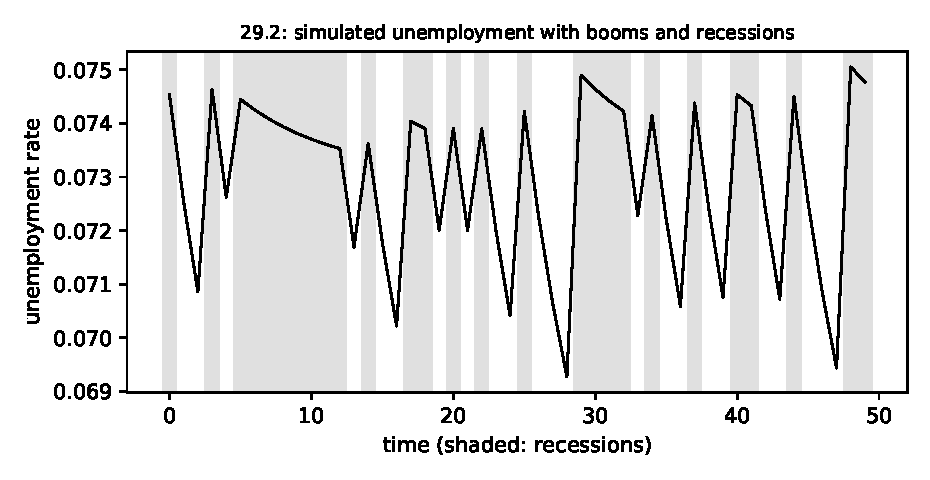
\includegraphics[width=0.6\textwidth]{figures/ch29_02.pdf}\\
{\small Figure S29.1.  Exercise 29.2: simulated unemployment with i.i.d.\ booms and recessions (shaded).}
\end{center}
\end{ex}

%%---------------------------------------------------------------------------
\begin{ex}{29.3}{Business cycles and search again}
\textbf{(a)}  Let $F_R=F$ and $F_B=F^2$ (the c.d.f.\ of the better of two draws), and $\tilde\beta=\beta(1-\mu)$.  A worker holding wage $w$ at the start of state $s$ has
\[
  V_s(w)=\max\Bigl\{\underbrace{w+\tilde\beta E_{s'}V_{s'}(w)}_{W(w)},\ \underbrace{b+\tilde\beta\int E_{s'}V_{s'}(w')\dd F_s(w')}_{Q_s}\Bigr\}.
\]
The value of working, $W(w)$, is the same in both states.  The value of searching depends on the state only through the offer distribution.

\textbf{(b)}  $F^2\le F$, so $F_B$ first-order dominates $F_R$.  Since $E_{s'}V_{s'}$ is nondecreasing (and increasing above the reservation wages), $Q_B>Q_R$.  With $W$
increasing, the reservation wages $W(\bar w_s)=Q_s$ satisfy $\bar w_B>\bar w_R$.  Employed workers with wages in $[\bar w_R,\bar w_B)$ keep their jobs in recessions but
\emph{quit when a boom arrives}, because jobs are more plentiful then.  Workers above $\bar w_B$ never quit.  Quits are procyclical here, the opposite of Exercise 29.2,
where the bonus $z$ made searching expensive in booms.  Unemployed workers are also choosier in booms.  Whether unemployment rises or falls in a boom depends on how the
extra draw raises job finding relative to the quits it triggers.
\end{ex}

%%---------------------------------------------------------------------------
\begin{ex}{29.4}{Skill-biased technological change (Mortensen and Pissarides)}
\textbf{(a)}  Apply (29.3.14) to market $i$ with $y=h_i$, $z=b$ and vacancy cost $ch_i$, and divide by $h_i$:
\[
  1-\frac b{h_i}=\frac{r+s+\varphi\theta_iq(\theta_i)}{(1-\varphi)q(\theta_i)}\,c,\qquad u_i=\frac{s}{s+\theta_iq(\theta_i)} .
\]
The right side increases in $\theta_i$.  With $b>0$, $\theta_i$ therefore increases with $h_i$, and $u_i$ falls with skill: vacancy costs scale with productivity but the outside
option $b$ does not, so the surplus share left after $b$ grows with skill.  The market for skill $h_i\le b$ shuts down ($\theta_i=0$, $u_i=1$).  With $b=0$, $\theta$ and $u$ do not
depend on $h$.  (We use the book's timing.  The exercise's separations at the start of a period change only the flow-balance details.)

\textbf{(b)}  Parameters (monthly): $r=.004$, $s=.02$, $\alpha=\varphi=.5$, $A=.35$ and $c=.65$, which give $u=6\%$ at $h=1$, $b=.4$.  Skills are uniform on $[1-D,1+D]$, so $D$
indexes mean-preserving spreads.
\begin{center}
\begin{tabular}{lcccc}
\toprule
aggregate $u$ (\%) & $D=0$ & $D=.2$ & $D=.4$ & $D=.6$\\
\midrule
$b=0$  & 4.64 & 4.64 & 4.64 & 4.64\\
$b=.2$ & 5.19 & 5.21 & 5.24 & 5.34\\
$b=.4$ & 6.00 & 6.05 & 6.22 & 7.61\\
$b=.6$ & 7.36 & 7.55 & 9.62 & 24.05\\
\bottomrule
\end{tabular}
\end{center}
Since $u_i$ is a decreasing, convex function of $h_i$ when $b>0$, spreads raise aggregate unemployment.  The effect grows sharply with $b$, as the least skilled
markets approach $h_i=b$ (Figure S29.2, left).  Skill-biased change interacts with generous benefits to produce European-style unemployment.

\textbf{(c)}  With $b_i=\rho h_i$ the left side becomes $1-\rho$ for every skill.  Tightness and unemployment are then the same in all markets, and mean-preserving spreads have
no effect ($u=6.00\%$ for $\rho=.4$).  The interaction in (b) arises because a fixed benefit is relatively more generous for low-skill workers.
\end{ex}

%%---------------------------------------------------------------------------
\begin{ex}{29.5}{Dispersion of match values (Marimon and Zilibotti)}
\textbf{(a)}  The match surplus is $S(p)=[p\bar h-(1-\beta)U]/(1-\beta(1-s))$, where $(1-\beta)U$ is the flow value of unemployment.  Matches form iff $p\ge p^*$, with
$p^*\bar h=(1-\beta)U$.  Nash bargaining gives $E(p)-U=\varphi S(p)$ and $J(p)=(1-\varphi)S(p)$, and the wage $w(p)=\varphi p\bar h+(1-\varphi)p^*\bar h$.  Free entry, with
vacancy cost $c\bar h$, and the value of unemployment give
\[
  q(\theta)=\frac{c\,(r+s)}{(1-\varphi)\int_{p^*}^\infty(p-p^*)\dd G(p)},\qquad p^*=\frac b{\bar h}+\frac{\varphi\,\theta c}{1-\varphi}.
\]
These two equations determine $(p^*,\theta)$.  (The second is the analogue of (29.3.12), and it follows from $(1-\beta)U=b+\beta\theta q\varphi\int_{p^*}S\dd G$ and free
entry.)  Steady-state unemployment is $u=s/[s+\theta q(\theta)(1-G(p^*))]$: job finding requires both a meeting and an acceptable draw.

\textbf{(b)}  Take $\bar h=1$, $\log p\sim N(-\sigma^2/2,\sigma^2)$ (mean one), and the matching parameters of 29.4.
\begin{center}
\begin{tabular}{lcccc}
\toprule
$u$ (\%) & $\sigma=.05$ & $\sigma=.3$ & $\sigma=.55$ & $\sigma=.8$\\
\midrule
$b=0$  & 4.71 & 9.87 & 15.17 & 20.29\\
$b=.4$ & 6.31 & 13.80 & 19.28 & 23.88\\
$b=.6$ & 8.13 & 17.20 & 22.12 & 26.05\\
$b=.8$ & 12.87 & 22.59 & 25.72 & 28.53\\
\bottomrule
\end{tabular}
\end{center}
Greater dispersion raises the option value of search: $\int_{p^*}(p-p^*)\dd G=E(p-p^*)^+$ rises under mean-preserving spreads, because $(p-p^*)^+$ is convex in $p$.  So
the reservation productivity rises,
more meetings are rejected, and unemployment rises even though tightness may increase.  Higher benefits raise $p^*$ further.  Over the empirically relevant range
of moderate dispersion, the rise in unemployment from $\sigma=.05$ to $.3$ is $5.2$ points with $b=0$ but $9.1$ with $b=.6$ (Figure S29.2, middle).  The employed
earn more, since only good matches survive, but at the cost of longer unemployment.
\end{ex}

%%---------------------------------------------------------------------------
\begin{ex}{29.6}{Idiosyncratic shocks to human capital (Ljungqvist and Sargent)}
\textbf{(a)}  The states are $(w,h)$ for the employed and $(b,h)$ for the unemployed, where $b$ is the benefit.  Workers survive each period with probability $1-\delta$ and are
replaced by unemployed newcomers with $(0,h_1)$, and $\tilde\beta=\beta(1-\delta)$.  We assume quitters forfeit benefits.  Then
\begin{align*}
  W(w,h)&=\max\bigl\{wh+\tilde\beta K(w,h),\ U(0,h)\bigr\},\\
  K(w,h)&=(1-s)\bigl[\pi_eW(w,h)+(1-\pi_e)W(w,h_2)\bigr]+s\bigl[\pi_uU(\gamma wh,h)+(1-\pi_u)U(\gamma wh,h_1)\bigr],\\
  U(b,h)&=b+\tilde\beta\int\max\{W(w',h),U(b,h)\}\dd G(w').
\end{align*}
An unemployed worker accepts $w'$ iff $w'\ge\bar w(b,h)$, where $W(\bar w,h)=U(b,h)$.  The reservation wage rises with $b$.  A stationary equilibrium is a solution of these
equations together with the invariant distribution over employed $(w,h)$ and unemployed $(b,h)$ that the decision rules and shocks induce.  The key state is a worker who was
laid off from a good job, lost skills, and draws benefits $\gamma wh_2$ while he can now earn only $w'h_1$.

\textbf{(b)}  Parameters (monthly): $\beta=.995$, $\delta=.002$ (a 40-year working life), $s=.02$, $\pi_e=.99$ (slow reskilling), $1-\pi_u=.8$, $G$ uniform on $[0,1]$ (100
points) and $h_2=1$.  Steady-state unemployment in percent:
\begin{center}
\begin{tabular}{lccccccc}
\toprule
$h_1$ & 1 & .9 & .8 & .7 & .6 & .5 & .4\\
\midrule
$\gamma=0$  & 9.5 & 9.6 & 9.6 & 9.6 & 9.6 & 9.5 & 9.3\\
$\gamma=.3$ & 11.3 & 11.3 & 11.3 & 11.3 & 11.3 & 11.4 & 11.4\\
$\gamma=.5$ & 13.1 & 13.2 & 13.3 & 13.4 & 13.7 & 14.4 & 16.8\\
$\gamma=.7$ & 16.6 & 16.7 & 17.4 & 19.4 & 61.3 & 72.3 & 74.7\\
\bottomrule
\end{tabular}
\end{center}
Without benefits, turbulence (a lower $h_1$) barely affects unemployment: skill losers simply accept lower earnings.  With generous earnings-related benefits it is
explosive.  Once $\gamma wh_2$ exceeds what a skill loser can earn, laid-off high earners rarely accept any job and stay unemployed until they retire (Figure S29.2,
right).  In calm times ($h_1$ near $h_2$) the welfare state works well.  In turbulent times the same benefits produce mass long-term unemployment.

\textbf{(c)}  All three models attribute high European unemployment to generous benefits in a more dispersed environment, through different channels.
\emph{29.4:} a fixed benefit shuts down low-skill markets.  The low tail of earnings is missing among the employed, which compresses measured earnings dispersion, while low-skill
unemployment soars.  Every unemployed worker has a constant hazard, so declining hazards appear only through composition across skill groups.  \emph{29.5:} benefits raise the
reservation match quality, truncating the wage distribution from below (less dispersion) and lengthening spells.  Again there is no true duration dependence.  \emph{29.6}
explains both facts best.  Skill losers with benefits tied to past earnings are extremely choosy, so they accept few low-paying jobs, and wage dispersion among the employed
rises less than in the U.S., where turbulence is absorbed by lower wages.  They also pile up in the unemployment pool.  The pool's composition shifts toward them with
duration, so the aggregate hazard falls sharply with duration: long-term unemployment.

\textbf{(d)}  In 29.4 and 29.5 a worker's situation is stationary: his prospects do not change with age or with his employment history.  A finite life only adds a constant
hazard of exit, which acts like a slightly lower discount factor, and steady states are essentially unchanged.  In 29.6, benefits indexed to past earnings create
(nearly) absorbing states: a skill loser whose benefit exceeds any wage he can earn never works again.  With infinite lives these workers accumulate forever, and steady-state
unemployment would be determined entirely by the mass that eventually falls into such states (in the limit, everyone).  With finite lives they leave through retirement.
Unemployment then depends on working-life length and on age: older workers with fewer years left to recover skills are even choosier.  Life-cycle structure is therefore
essential for the quantitative results.
\begin{center}
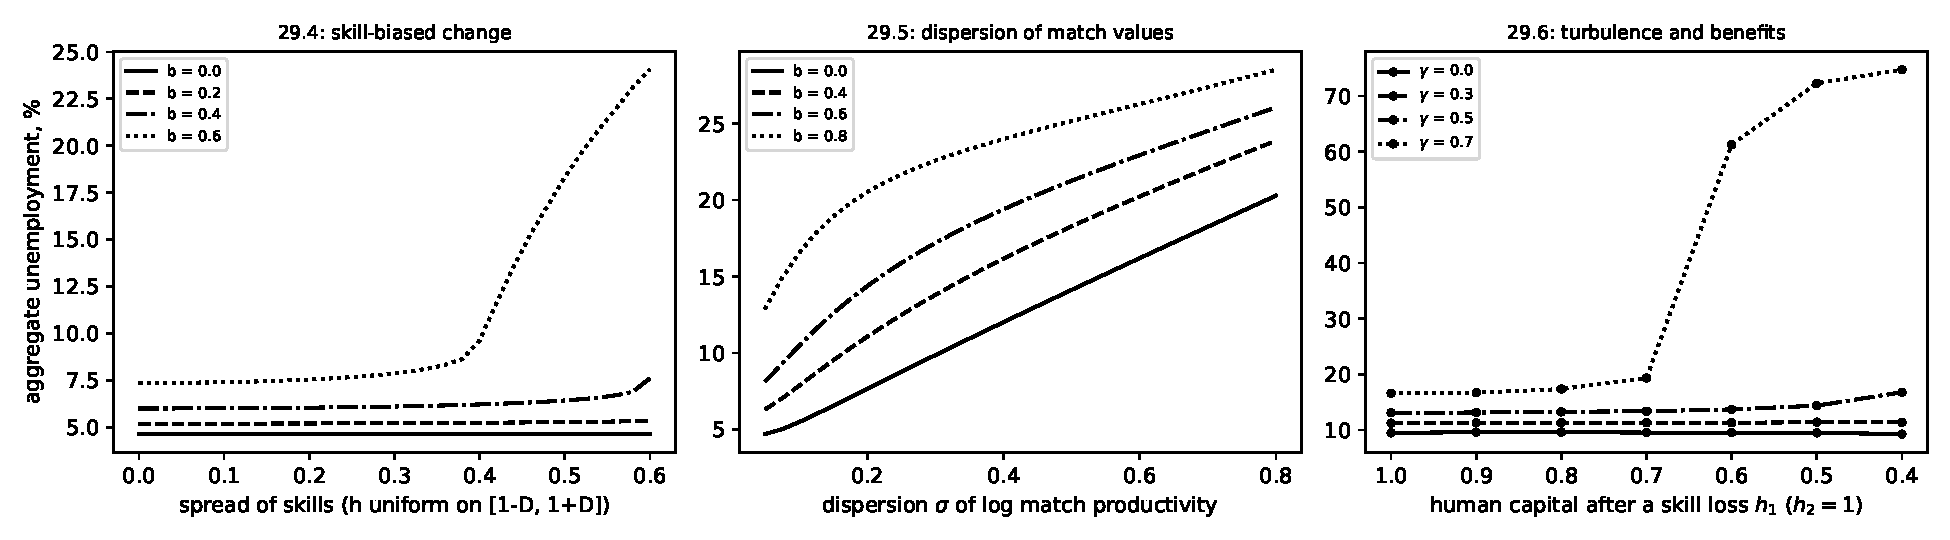
\includegraphics[width=\textwidth]{figures/ch29_04.pdf}\\
{\small Figure S29.2.  Steady-state unemployment in Exercises 29.4 (mean-preserving spreads of skills), 29.5 (dispersion of match productivity) and 29.6 (turbulence: lower
human capital after a skill loss), for several benefit levels.}
\end{center}
\end{ex}

%%---------------------------------------------------------------------------
\begin{ex}{29.7}{Temporary jobs and layoff costs}
\textbf{(a)}  Let $Q$ be the value of drawing a new wage (unemployed this period).  A job at $w$ that is never quit is worth $E(w)=w+\beta[(1-\mu)E(w)+\mu Q]$, i.e.\
$E(w)=(w+\beta\mu Q)/(1-\beta(1-\mu))$.  A worker holding $w$ works iff $E(w)\ge Q$, i.e.\ iff $w\ge\bar w=(1-\beta)Q$.  From
$Q=b+\beta\int\max\{E(w'),Q\}\dd F(w')$,
\[
  \bar w=b+\frac{\beta}{1-\beta(1-\mu)}\int_{\bar w}^M(w-\bar w)\dd F(w).
\]
Unemployed workers accept offers above $\bar w$ and employed workers never quit.  Shorter jobs (higher $\mu$) lower the reservation wage.

\textbf{(b)}  No.  With both types, $E(w,\mu)=(w+\beta\mu Q)/(1-\beta(1-\mu))\ge Q$ iff $w\ge(1-\beta)Q$, for either $\mu$.  (Here $Q$ averages over both types of offers.)  A job is
worth taking iff its flow $w$ beats the flow value of search $(1-\beta)Q$.  Its duration only scales how long that gain lasts, and when the job ends the worker is back to
searching anyway.  Duration affects the value of a good job but not whether it is good.

\textbf{(c)}  With the layoff cost, a job that is never quit is worth $E(w)=[w+\beta\mu(Q-\tau)]/(1-\beta(1-\mu))$.  (i) An unemployed worker holding an offer accepts iff
$E(w)\ge Q$, i.e.\ $w\ge\bar w_u=(1-\beta)Q+\beta\mu\tau$.  (ii) An employed worker continues iff $E(w)\ge Q-\tau$, since quitting costs $\tau$, i.e.\
$w\ge\bar w_e=(1-\beta)(Q-\tau)$.  So $\bar w_u-\bar w_e=\tau(1-\beta+\beta\mu)>0$.  Unemployed workers are choosier because accepting a job commits them to a future layoff cost.
Employed workers are more reluctant to quit because quitting costs $\tau$ now.  Since accepted wages exceed $\bar w_u>\bar w_e$, no one quits.

\textbf{(d)}  $\bar w_u(\mu)=(1-\beta)Q+\beta\mu\tau$ increases with $\mu$, so $\bar w_s=\bar w_u(\mu_s)>\bar w_l=\bar w_u(\mu_l)$.  A short-lasting job brings the layoff cost
sooner in expected present value, so it must pay more to be accepted.  Layoff costs thus tilt acceptance toward long-lasting jobs.

\textbf{(e)}  Employed workers at the start of $t+1$ lose their jobs with probability $\mu_i$.  Unemployed workers at $t$ draw an offer that starts at $t+1$ if accepted, and a new
hire does not face the loss draw in her first period.  Hence
\begin{align*}
  N_{s,t+1}&=(1-\mu_s)N_{st}+\pi_s\bigl[1-F(\bar w_s)\bigr]U_t,\qquad N_{l,t+1}=(1-\mu_l)N_{lt}+\pi_l\bigl[1-F(\bar w_l)\bigr]U_t,\\
  U_{t+1}&=\mu_sN_{st}+\mu_lN_{lt}+\Bigl[1-\pi_s\bigl(1-F(\bar w_s)\bigr)-\pi_l\bigl(1-F(\bar w_l)\bigr)\Bigr]U_t ,
\end{align*}
which preserve $N_{st}+N_{lt}+U_t=1$.
\end{ex}

%%---------------------------------------------------------------------------
\begin{ex}{29.8}{Productivity shocks, job creation, and job destruction (Manuelli)}
\textbf{(a)}  A filled job is worth $J=y-w+\beta[sV+(1-s)J]$, and a vacancy $V=-c+\beta[qJ+(1-q)V]$.  With $V=0$, $J=c/(\beta q)$.  Then
$(y-w)/(1-\beta(1-s))=c/(\beta q)$, and since $(1-\beta(1-s))/\beta=r+s$, $w=y-(r+s)c/q(\theta)$.

\textbf{(b)}  This is (29.3.13).  Nash bargaining gives $E-U=\varphi S$ and $J=(1-\varphi)S$.  The worker's value of unemployment satisfies $rU/(1+r)=z+\varphi\theta c/(1-\varphi)$
(29.3.12), and the wage is the annuity value of unemployment plus the share $\varphi$ of the one-period surplus.  Together these give $w=z+\varphi(y-z+\theta c)$.

\textbf{(c)}  Equating the two wage expressions gives (29.3.14),
$y-z=\bigl[(r+s+\varphi\theta q(\theta))/((1-\varphi)q(\theta))\bigr]c$.  The right side increases continuously in $\theta$ (because $q'<0$ and $\theta q$ increases).  So there is a
unique $\theta$, increasing in $y-z$ and decreasing in $c$, $r$, $s$ and $\varphi$.  Unemployment then follows from $u=s/(s+\theta q(\theta))$.

\textbf{(d)}  A higher $y$ raises the left side, so $\theta'>\theta$.  In the dynamic economy, free entry must hold every period, $c=\beta q(\theta_t)J_{t+1}$, with
$J_t=y'-w_t+\beta(1-s)J_{t+1}$ and a Nash wage that depends on $\theta_t$.  None of these equations involves the unemployment rate.  With constant returns to matching, the
value of a vacancy depends only on the ratio $\theta$, not on the levels of $u$ and $v$.  Vacancies can be opened or closed instantly.  Unemployment is the only slow-moving
state variable, and it does not feed back into $\theta$.  The only non-explosive solution of the forward-looking free-entry recursion is therefore $\theta_t=\theta'$ from
$t=0$ on: tightness jumps, and vacancies jump to $v_0=\theta'u_0$.

\textbf{(e)}  Before the shock, $JC=JD=s(1-u_0)$ with $u_0=s/(s+\theta q(\theta))$.  At $t=0$ job destruction is unchanged, $JD_0=s(1-u_0)$, while job creation jumps to
$JC_0=\theta'q(\theta')u_0>s(1-u_0)$.  Afterwards $u_{t+1}=u_t+s(1-u_t)-f'u_t$ with $f'=\theta'q(\theta')$, so
\[
  u_t-u'=(1-s-f')^t(u_0-u'),\qquad u'=\frac{s}{s+f'} .
\]
Unemployment falls monotonically to $u'$.  Job creation $JC_t=f'u_t$ falls after its initial spike, and job destruction $JD_t=s(1-u_t)$ rises as employment grows.  Both converge to
$s(1-u')$, with $JC_t>JD_t$ throughout the transition.  Vacancies $v_t=\theta'u_t$ overshoot on impact and then decline with $u_t$.  (Example: $y=1\to1.05$, $z=.4$ and the
calibration of 29.4.  Then $\theta$ jumps from $.800$ to $.872$, the job-finding rate from $.313$ to $.327$, and $u$ falls from $6.00\%$ to $5.77\%$.  $JC$ jumps from $.0188$ to
$.0196$ and then declines, while $JD$ rises slowly from $.0188$.)
\end{ex}

%%---------------------------------------------------------------------------
\begin{ex}{29.9}{Workweek restrictions, unemployment, and welfare (Manuelli)}
\textbf{(a)}  A match produces $yx+z(1-x)$, compared with $z$ for an unmatched worker, so its flow surplus is $(y-z)x$.  Since $x$ is observed, the pair chooses it to maximize
the surplus, and Nash bargaining then splits it: $x=1$ because $y>z$.  The equilibrium is that of 29.8: $\theta$ solves (29.3.14), $w=z+\varphi(y-z+\theta c)$, and
$u=s/(s+\theta q(\theta))$.

\textbf{(b)}  With $q=A\theta^{-\alpha}$, the elasticity of $q$ is $-\alpha$, and the planner's condition is (29.3.19).  The market equilibrium is efficient iff $\varphi=\alpha$ (the
Hosios condition).  If $\varphi>\alpha$ there are too few vacancies; if $\varphi<\alpha$, too many.

\textbf{(c)}  The cap binds ($x=x^*$), since the surplus increases in $x$.  Free entry now reads $(y-w)x^*=(r+s)c/q(\theta)$, where $w$ is the hourly wage.  The same steps as in
29.8, applied to the flow surplus $(y-z)x^*$, give $w=z+\varphi(y-z)+\varphi\theta c/x^*$ and
\[
  y-z=\frac{r+s+\varphi\theta q(\theta)}{(1-\varphi)q(\theta)}\cdot\frac{c}{x^*} .
\]
The cap acts like raising the vacancy cost from $c$ to $c/x^*$: each vacancy now brings a smaller flow of output.

\textbf{(d)}  The right side increases in $\theta$, so tightness falls.  The job-finding rate $\theta q(\theta)$ falls, unemployment $u=s/(s+\theta q(\theta))$ rises, and the number
of jobs $1-u$ falls.  The hourly wage $w=z+\varphi(y-z)+\varphi\theta c/x^*$ also falls.  With $q=A\theta^{-\alpha}$, the equilibrium condition gives
$(y-z)(1-\varphi)=(\theta c/x^*)[(r+s)\theta^{\alpha-1}/A+\varphi]$, and as $c/x^*$ rises $\theta$ falls, so $\theta^{\alpha-1}$ rises and $\theta c/x^*$ must fall.  Weekly earnings
$wx^*$ fall by more.  The cap does not share work.  It destroys match surplus, so fewer jobs are created, and welfare falls.  The equilibrium is not optimal: the planner would
choose $x=1$.  Given the cap, the allocation is constrained efficient only if $\varphi=\alpha$.
\end{ex}

%%---------------------------------------------------------------------------
\begin{ex}{29.10}{Costs of creating a vacancy and optimality (Manuelli)}
\textbf{(a)}  Firms take $p_A$ as given, so free entry gives $y-w=(r+s)C'(v)/q(\theta)$.  The Nash wage is $w=z+\varphi(y-z+\theta C'(v))$, because the cost of a vacancy enters
the worker's outside option as in (29.3.12).  In a steady state $v=\theta u=s\theta/(s+\theta q(\theta))$, which increases in $\theta$.  Hence $\theta$ solves
\[
  y-z=\frac{r+s+\varphi\theta q(\theta)}{(1-\varphi)q(\theta)}\,C'\!\Bigl(\frac{s\theta}{s+\theta q(\theta)}\Bigr),
\]
whose right side increases in $\theta$, so the solution is unique.  A higher $y$ or lower $z$ raises $\theta$ and vacancies and lowers unemployment.  A steeper (or higher) $C'$
lowers $\theta$.  Because the supply of vacancies is less than perfectly elastic, shocks to $y-z$ move $\theta$ and $u$ less than with a constant $c$, and part of each shock
shows up in the price $p_A$.

\textbf{(b)}  The planner maximizes $\sum\beta^t[yn_t+z(1-n_t)-C(v_t)]$ subject to $n_{t+1}=(1-s)n_t+q(v_t/(1-n_t))v_t$.  With $q=A\theta^{-\alpha}$ (so $q+q'\theta=(1-\alpha)q$ and
$q'\theta^2=-\alpha\theta q$), the stationary first-order conditions give
\[
  y-z=\frac{r+s+\alpha\theta q(\theta)}{(1-\alpha)q(\theta)}\,C'(v).
\]
This is the market condition with $\alpha$ in place of $\varphi$: the marginal social cost of a vacancy, $C'(v)$, equals its market price.  The equilibrium is efficient iff
$\varphi=\alpha$, the Hosios condition, and inefficient otherwise.
\end{ex}

%%---------------------------------------------------------------------------
\begin{ex}{29.11}{Financial wealth, heterogeneity, and unemployment (Manuelli)}
Each period an unemployed worker draws an offer, which he can take up at once.  Otherwise he consumes $a$ out of wealth.  With linear utility and $1+r=\beta^{-1}$, the
timing of consumption is irrelevant, and a worker's value is his wealth plus the present value of his earnings.  So rejecting an offer costs exactly one period of wage income.

\textbf{(a)}  A type-0 worker has no wealth and cannot finance the minimum consumption for a period of search.  He must take the first offer, so $w^*(0)=a$, the bottom of the
support.

\textbf{(b)}  A type-1 worker can afford one period of search and then becomes type 0.  Accepting $w$ yields $w/(1-\beta)$ in earnings; waiting yields $\beta\bar w/(1-\beta)$.
Hence $w^*(1)=\beta\bar w>a$ by assumption.  A type-2 worker who waits becomes type 1 (his wealth $a\beta$ grows to $a$).  So
$w^*(2)=\beta E\max\{w,w^*(1)\}>\beta E w=w^*(1)$, strictly because $F(w^*(1))>0$.  Wealthier workers are choosier: across workers, financial wealth and
unemployment duration are positively related, and employment probabilities fall with wealth.  Wealth finances search, which liquidity constraints otherwise rule
out.  The poor take the first job, and the wealthy hold out for better wages.

\textbf{(c)}  Count as unemployed in period $t$ everyone without a job at the start of $t$.  These are the newborns $nN_{t-1}$, the type-1 and type-2 workers born at $t-1$ who
rejected ($F_1=F(w^*(1))$, $F_2=F(w^*(2))$), and the type-2 workers born at $t-2$ who rejected twice and must now accept.  With $\varphi_2=1-\varphi_0-\varphi_1$ and $N_t=(1+n)N_{t-1}$,
\[
  u_t=\frac{U_t}{N_t}=\frac n{1+n}\Bigl[1+\frac{\varphi_1F_1+\varphi_2F_2}{1+n}+\frac{\varphi_2F_2F_1}{(1+n)^2}\Bigr],
\]
which is constant: the population grows at a constant rate, and each cohort's unemployment profile is the same.

\textbf{(d)}  Moving mass from type 0 to type 1 raises $u$ by $\frac n{(1+n)^2}F_1$ per unit.  Moving mass from type 1 to type 2 raises it by
$\frac n{1+n}\bigl[\frac{F_2-F_1}{1+n}+\frac{F_2F_1}{(1+n)^2}\bigr]>0$ per unit.  So redistributing wealth toward the richer types raises unemployment, while it also raises the
average accepted wage.  Transfers to the poorest ($\varphi_0$ down) raise measured unemployment and wages, since they give workers the means to search.  Redistribution
from type 2 to type 0 lowers unemployment, but it also lowers wages.
\emph{Extra credit.}  A type-2 worker is unemployed for $D=1$ period with probability $1-F_2$ (he accepts at birth), $D=2$ with probability $F_2(1-F_1)$, and $D=3$ with
probability $F_2F_1$ (after two rejections he must accept).  So $E D=1+F_2+F_2F_1$, and the hazard of leaving unemployment rises with duration, to one in the third period,
as his wealth runs down.
\end{ex}

\end{document}
